\documentclass[lang=cn,10pt,scheme=chinese,color=blue,usesamecnt]{asymptoticbook}

\title{渐近统计笔记}
% \subtitle{概率极限定理、统计估计与 Bootstrap}

\author{\href{https://www.zhihu.com/people/he-eeeeeeeee}{金鱼马}}
\date{2026年9月}
\institute{浙江大学}
\bioinfo{License}{\href{https://creativecommons.org/licenses/by-nc-sa/4.0/deed.en}{CC BY-NC-SA 4.0}}

% ElegantBook 没有内置教师字段；在主文件中扩展封面信息，避免修改模板类文件。
\makeatletter
\newcommand{\teacher}[1]{\gdef\@teacher{#1}}
\newcommand{\teachername}{\citshape 授课教师：}
\patchcmd{\maketitle}
  {\ifcsname @institute\endcsname \institutename \cnormal\@institute\\ \fi}
  {\ifcsname @institute\endcsname \institutename \cnormal\@institute\\ \fi
   \ifcsname @teacher\endcsname \teachername \cnormal\@teacher\\ \fi}
  {}
  {\PackageWarning{asymptotic-statistics}{Failed to add the teacher field to the title page}}
\makeatother
\teacher{\href{https://jia-gu.github.io/}{顾嘉}}

\cover{figures/cover2.jpg}

\usepackage{bm}
\usepackage{mathtools}
\mathtoolsset{showonlyrefs}
\usepackage{mathrsfs}
\usepackage{dsfont}
\usepackage{booktabs}
\usepackage{longtable}
\usepackage{microtype}
\usepackage{csquotes}
\definecolor{DarkRed}{HTML}{8B1E2D}
\renewcommand{\examplename}{例}
\renewcommand{\assumptionname}{条件}

\addbibresource[location=local]{references.bib}
\setcounter{tocdepth}{1}
\numberwithin{equation}{chapter}
\providecommand{\tightlist}{%
  \setlength{\itemsep}{0pt}\setlength{\parskip}{0pt}%
}
\newcommand{\chapterreferences}{%
  \printbibliography[heading=subbibliography,title={本章参考文献}]%
}
\makeatletter
\newcommand{\extensionchapter}[3]{%
  \chapter*{#1}%
  \phantomsection
  \addcontentsline{toc}{chapter}{#1}%
  \label{#2}%
  \setcounter{equation}{0}%
  \renewcommand{\theequation}{#3.\arabic{equation}}%
  \renewcommand{\theHequation}{#3.\arabic{equation}}%
  \setcounter{ELEGANT@samecnt}{0}%
  \renewcommand{\theELEGANT@samecnt}{#3.\arabic{ELEGANT@samecnt}}%
  \renewcommand{\theHELEGANT@samecnt}{#3.\arabic{ELEGANT@samecnt}}%
  \setcounter{exam}{0}%
  \renewcommand{\theexam}{#3.\arabic{exam}}%
  \renewcommand{\theHexam}{#3.\arabic{exam}}%
  \setcounter{section}{0}%
  \setcounter{subsection}{0}%
  \setcounter{subsubsection}{0}%
  \renewcommand{\thesection}{#3.\arabic{section}}%
  \renewcommand{\theHsection}{#3.\arabic{section}}%
  \renewcommand{\thesubsection}{#3.\arabic{section}.\arabic{subsection}}%
  \renewcommand{\theHsubsection}{#3.\arabic{section}.\arabic{subsection}}%
  \renewcommand{\thesubsubsection}{#3.\arabic{section}.\arabic{subsection}.\arabic{subsubsection}}%
  \renewcommand{\theHsubsubsection}{#3.\arabic{section}.\arabic{subsection}.\arabic{subsubsection}}%
}
\makeatother

% 让各定理类 tcolorbox 的标题编号实时跟随 \theELEGANT@samecnt（默认它在框体创建时被固化一次）。
\makeatletter
\newcommand{\extensiontheoremtitle}{%
  \expandafter\def\csname thetcb@cnt@theorem\endcsname{\theELEGANT@samecnt}%
  \expandafter\def\csname thetcb@cnt@definition\endcsname{\theELEGANT@samecnt}%
  \expandafter\def\csname thetcb@cnt@proposition\endcsname{\theELEGANT@samecnt}%
  \expandafter\def\csname thetcb@cnt@lemma\endcsname{\theELEGANT@samecnt}%
  \expandafter\def\csname thetcb@cnt@corollary\endcsname{\theELEGANT@samecnt}%
  \expandafter\def\csname thetcb@cnt@axiom\endcsname{\theELEGANT@samecnt}%
  \expandafter\def\csname thetcb@cnt@postulate\endcsname{\theELEGANT@samecnt}%
}
\extensiontheoremtitle
\makeatother

\renewcommand{\thesection}{\arabic{chapter}.\arabic{section}} % 例如 1.1
\renewcommand{\thesubsection}{\thesection.\arabic{subsection}} % 例如 1.2.1
\renewcommand{\thesubsubsection}{\thesubsection.\arabic{subsubsection}} % 例如 1.2.1.1

\begin{document}

\maketitle
\frontmatter
\tableofcontents

\chapter*{关于本笔记}
\phantomsection
\addcontentsline{toc}{chapter}{关于本笔记}
本文是个人整理的浙江大学 2025--2026 学年春夏学期研究生课程《统计中的逼近理论》笔记。
授课教师为浙江大学数据科学研究中心的\href{https://jia-gu.github.io/}{顾嘉}老师。
笔记内容也发布在\href{https://zhuanlan.zhihu.com/p/1973423321602348153}{知乎专栏}。

课程以渐近统计的理论基础为主，涉及随机收敛、特征函数、中心极限定理、弱相依数据、Delta 方法、矩估计、极大似然估计、经验似然、M-估计与 Z-估计、U-统计量以及 Bootstrap，共十一章。
此外，笔者补充了“稳定分布与无限方差中心极限定理”和“泛函中心极限定理”两篇扩展阅读。

课程使用的教材为 van der Vaart 的 \emph{Asymptotic Statistics}。其它可参考教材包括：
\begin{itemize}
\item Serfling 的 \emph{Approximation Theorems in Mathematical Statistics}；
\item Durrett 的 \emph{Probability: Theory and Examples}；
\item Ferguson 的 \emph{A Course in Large Sample Theory}；
\item White 的 \emph{Asymptotic Theory for Econometricians}；
\item van der Vaart 与 Wellner 的 \emph{Weak Convergence and Empirical Processes}；
\item Bosq 的 \emph{Nonparametric Statistics for Stochastic Processes}；
\item Bijma、Ern\'e、Jonker 与 van der Vaart 的 \emph{An Introduction to Mathematical Statistics}。
\end{itemize}

本笔记并非官方课程材料；文中的疏漏与错误由笔者负责。欢迎向作者报告公式、证明、引用或排版问题。

\mainmatter

\begin{refsection}
\chapter{随机收敛}\label{ch:random-convergence}
% Generated from: Zhihu/专栏：概率与统计/渐近统计 (1) ：随机收敛_金鱼马_2026-04-29.md
为什么要学渐近统计？在很多时候，在固定样本，或者说非渐近 (non-asymptotic) 下，找到一个统计量的具体分布，或者进行精确的分析，往往是非常困难的。有可能是因为统计量的分布非常复杂、难以解析求解，也可能是我们的统计模型与真实分布之间存在偏差。

这时，让样本量 $n\to\infty$ 可以使问题得到简化，通常能得到对统计量分布的非常好的近似，并得到一个非常简洁的渐近分布（如正态分布）。渐近近似有很多用途：我们可将之用于渐近推断，如寻找近似的置信域和检验；也可用于从理论上研究统计推断方法的优劣，如有效性 (efficiency)。

我们首先介绍随机变量的收敛。

\begin{definition*}[随机变量、随机向量与分布函数]
对于给定的概率空间 $(\Omega,\mathscr F,P)$，（实值）随机变量定义为
$(\Omega,\mathscr F,P)\to(\mathbb R,\mathscr B_{\mathbb R})$ 的 Borel 可测映射；
$k$ 维随机向量是
\[
X=(X_1,X_2,\dots,X_k):
(\Omega,\mathscr F,P)\to(\mathbb R^k,\mathscr B_{\mathbb R^k})
\]
的 Borel 可测映射。随机向量 $X$ 的分布函数 (CDF) 定义为
\[
F_X(x):=P(X\le x)
=P(X_1\le x_1,X_2\le x_2,\dots,X_k\le x_k).
\]
\end{definition*}

\section{收敛模式}

常见的随机变量的收敛有以下三种：
\begin{definition}
设 $\{X_n\}$ 为一列 $\mathbb{R}^k$ 上的随机向量，\[ d(x, y):=\|x-y\|=\left(\sum_{i=1}^k(x_i-y_i)^2\right)^{1/2} \]为 $\mathbb{R}^k$ 中的欧式距离，诸 $\{X_n\}, X$ 定义在同一个概率空间上，
\begin{itemize}
\tightlist
\item
  \textbf{\emph{几乎必然收敛}} ：如果 $d(X_n, X) \to 0$ 的概率为1：$P(\lim_{n} d(X_n, X) = 0) = 1$ ，那么称 $\{X_n\}$ 几乎必然 (almost surely) 收敛到 $X$，我们记作 $X_n \overset{\text{a.s.}}\to X$ 。

\begin{itemize}
  \tightlist
  \item
    —— 可理解为``100\% 确信 + 100\% 精确''。
  \end{itemize}
\item
  \textbf{依概率收敛} ：如果对任意 $\epsilon > 0$，都有 $\lim\limits_{n\to\infty} P(d(X_n, X) < \epsilon) = 1$，那么称 $\{X_n\}$ 依概率收敛到 $X$，记作 $X_n \overset{P}\to X$ 。

\begin{itemize}
  \tightlist
  \item
    —— 可理解为``100\% 确信 + 不100\% 精确''。
  \end{itemize}
\item
  \textbf{$r$ \emph{阶矩收敛}} ：如果 $\lim\limits_{n\to\infty} \mathbb E[(d(X_n, X))^r ]= 0$ ，那么称 $\{X_n\}$ 按 $r$ 阶矩收敛到 $X$ ，记作 $X_n\overset{L^r}\to X$ 。
\end{itemize}
\end{definition}

在渐近分析中，最常用的收敛是依分布收敛。相比于前面的三种收敛，依分布收敛不要求 $\{X_n\}, X$ 必须在同一个概率空间中定义，因为这种收敛只关心``分布''这一统计特征。

\begin{definition}
记随机向量 $X_n$ 的分布函数为 $F_n$ 、 $X$ 的分布函数为 $F$ ，如果在 $F$ 的所有连续点 $x$ 处都有\[\lim_{n\to \infty} F_n(x) = F(x)\]
则称 $X_n$ \textbf{\emph{依分布收敛 }}到 $X$ ，记作 $X_n\overset{\rm d}\to X$ 。依分布收敛也称作弱收敛 (weak convergence) 或者 convergence in law。也有的文献记作 $X_n\rightsquigarrow X$ 。
\end{definition}

\begin{remark}

\begin{itemize}
\tightlist
\item
  分布函数总是单调非降的，因此，根据 \href{https://en.wikipedia.org/wiki/Discontinuities_of_monotone_functions}{Froda 定理}， $F$ 不连续的点至多只有可数个。
\item
  如果 $X$ 有某种特殊分布，如标准正态分布 $\mathcal N(0,1)$ ，我们也可以记作 $X_n\overset{\rm d}\to\mathcal{N}(0,1)$ 。
\end{itemize}
\end{remark}

统计学中的``渐近分布''和``渐近正态''的概念就是建立在依分布收敛上的。其定义如下：

\begin{definition}\label{def:ch1:limit-distribution}
若一列 (一维) 随机变量 $\{X_n\}$ 满足：存在常数数列 $a_n$ 以及 $b_n>0$ 和某个 (非退化) 分布 $F$ ，使得 $\frac{X_n-a_n}{b_n}\overset{\rm d}\to F$
就称 $\{X_n\}$ 有\textbf{\emph{渐近分布}} (asymptotic distribution) $F$ 。特别地，当 $F$ 是标准正态分布 $\mathcal N(0,1)$ 时，称 $\{X_n\}$ 是\textbf{\emph{渐近正态}} (asymptotically normal) 的，形式上记作 $X_n\sim A\mathcal{N}(a_n,b_n^2)$ ，这里 $a_n$ 和 $b_n$ 可以视作其渐近意义上的均值和标准差--注意，只是渐近意义上的，例如， $X_n$ 本身的均值和方差不一定存在。

这个定义可以推广到高维：设 $\{X_n\}$ 是一列 $k$ 维随机向量，如果存在一列向量 $A_n\in \mathbb R^k$ 和正定矩阵 $B_n\in\mathbb R^{k\times k}$ ，以及一个 $k$ 维分布，使得 $B_n^{-1}(X_n-A_n)\overset{\rm d}\to F$
则称 $\{X_n\}$ 有渐近分布 $F$ ；当 $F$ 是 $k$ 维标准正态分布 $\mathcal N(\bm 0,\mathbf{I}_k)$ 时，称 $X_n$ 是渐近正态的。
\end{definition}

最后，值得一提的是，依概率收敛和依分布收敛都可以视作某种度量下的收敛。

\begin{itemize}
\tightlist
\item
  定义两个随机变量 $X,Y$ 的 \emph{Ky Fan 度量}为
  \[
  d_{\text{KF}}(X,Y):=\inf\big\{\epsilon>0:P(d(X,Y)>\epsilon)\le\epsilon\big\}.
  \]
  则 $X_n\overset P\to Y$ 当且仅当 $d_{\text{KF}}(X_n,Y)\to 0$。它与某些其它的度量等价，如 $d(X,Y)=\mathbb{E}[|X-Y|\wedge 1]$ 或者 $\mathbb{E}\left[\frac{|X-Y|}{1+|X-Y|}\right]$ 。%可见 \url{https://www.zhihu.com/question/666217506/answer/1919169708051116292}。
\item
  定义两个 (一维) 分布函数 $F,G:\mathbb R\to[0,1]$ 的 \emph{Lévy 度量 }为\[ d_{\rm L}(F,G):=\inf\big\{\epsilon >0:F(x-\epsilon )-\epsilon \leq G(x)\leq F(x+\epsilon )+\epsilon ,\;\forall x\in \mathbb {R}\big\} \]那么 $X_n\overset{\rm d}\to X$ 当且仅当 $d_{\rm L}(F_n,F)\to 0$ ，其中 $F_n,F$ 分别是 $X_n$ 和 $X$ 的分布函数。%参考 \url{https://math.stackexchange.com/questions/1774319/relationship-to-weak-toplogy-l\%c3\%a9vy-metric} 和 \href{https://en.wikipedia.org/wiki/L\%C3\%A9vy\%E2\%80\%93Prokhorov_metric}{Lévy--Prokhorov metric - Wikipedia}。
\end{itemize}

\section{弱收敛的刻画}

本节来介绍一下``依分布收敛''或者说``弱收敛''能蕴含哪些结论。
先补充一下测度角度``弱极限''的概念：
\begin{definition}\label{def:ch1:weak-convergence}
设有 Polish 空间 $\mathscr X$ 和上面的 Borel $\sigma$ -代数 $\mathscr B_x$ ， $P_n,P$ 是其上的(有限) 测度，如果对任意的有界连续函数 $f:\mathscr X\to \mathbb R$ 都有
\[
\int_{\mathscr X}f(x)\mathrm dP_n(x)\to \int_{\mathscr X}f(x)\mathrm dP(x),
\]
则称测度列 $\{P_n\}$ \emph{弱收敛}到 $P$ 。
\end{definition}
不难证明，如果测度的弱极限存在，则它是唯一的。下面的 \hyperref[thm:ch1:portmanteau]{Portmanteau 定理} 告诉我们，随机变量的依分布收敛就是它们诱导出的 $\mathbb R^k$ 上测度的弱收敛。

\subsection{Portmanteau 定理}

\textbf{\emph{Portmanteau 定理 }}最初由 A. D. Alexandroff 在 1941 年给出。``Portmanteau''一词指的是一种大型旅行包，意指此定理将几种不同但完全等价的依分布收敛的方式打包在一起；它为我们提供了一个工具箱：在证明依分布收敛时，只需证明其中之一。

\begin{theorem}[Portmanteau 定理]\label{thm:ch1:portmanteau}

\label{thm:ch1:1-1}

对任意 $k$ 维随机向量 $X_n$ 和 $X$，以下陈述等价。

\begin{enumerate}
\def\labelenumi{\arabic{enumi}.}
\tightlist
\item
  依分布收敛： $X_n \overset{\rm d}\to X$；
\item
  对所有有界连续函数 $f$，有 $\mathbb{E}[f(X_n)] \to \mathbb{E}[f(X)]$；
\item
  对所有有界 Lipschitz 函数 $f$ ，有 $\mathbb{E}[f(X_n)] \to \mathbb{E}[f(X)]$；
\item
  对所有非负连续函数 $f$，有 $\liminf\limits_{n\to\infty} \mathbb{E}[f(X_n)] \geq \mathbb{E}[f(X) ]$；
\item
  对任意开集 $G$，有 $\liminf\limits_{n\to\infty} P(X_n \in G) \geq P(X \in G)$；
\item
  对任意闭集 $F$，有 $\limsup\limits_{n\to\infty} P(X_n \in F) \leq P(X \in F)$；
\item
  对任意满足 $P(X \in \partial B) = 0$ 的 Borel 集 $B$，我们称之为\emph{连续集} (continuity set)，有 $P(X_n \in B) \to P(X \in B)$。这里 $\partial B:=\overline B\setminus B^\circ$ 代表 $B$ 的\emph{边界} (boundary)。
\end{enumerate}

\end{theorem}

\begin{proof}

我们的证明顺序如图~\ref{fig:ch1:portmanteau-proof-map} 所示：

\begin{figure}[htbp]
  \centering
  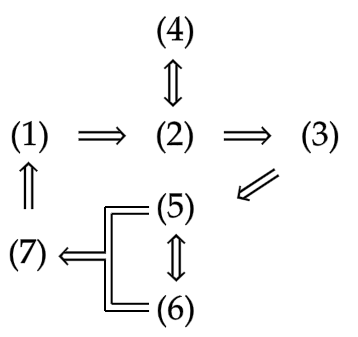
\includegraphics[width=0.4\textwidth]{figures/portmanteau-proof-map.png}
  \caption{Portmanteau 定理各条件之间的证明关系（Mathcha 绘制）}
  \label{fig:ch1:portmanteau-proof-map}
\end{figure}
\begin{itemize}[leftmargin=3cm]
  \item[(1.) $\Rightarrow$ (2.)] 不失一般性，可以设 $\sup_{x\in\mathbb R}|f(x)|\le 1$ 。先证明 $X$ 的分布函数 $F$ 连续的情形。对任意 $\epsilon>0$ ，我们可以找到足够大但有界的闭立方体 $I$ 使得 $P(X\not\in I)<\epsilon$ 。连续函数 $f$ 在紧集 $I$ 上是一致连续的，我们可以将 $I$ 划分成若干小立方体 $I=\bigcup_{j=1}^NI_j$ ，使得 $f$ 在每个 $I_j$ 上取值的差距都不超过 $\epsilon$ 。从每个 $I_j$ 中取一点 $x_j$ ，定义
  \[
  f_\epsilon(x):=\sum_{j=1}^Nf(x_j)\mathbb{I}(x\in I_j).
  \]

那么在 $I$ 上总有 $|f-f_\epsilon|<\epsilon$ 。由此得知，\[\begin{aligned} |\mathbb{E}[f(X)]-\mathbb{E}[f_\epsilon (X)]|&\le\mathbb{E}\big[|f(X)-f_\epsilon(X)|\mathbb{I}(X\in I)\big]+\mathbb{E}\big[|f(X)|\mathbb{I}(X\not\in I)\big]\\ &\le \epsilon+P(X\not\in I)\qquad {\scriptstyle |f(x)|\le 1}\\ &\le 2\epsilon \end{aligned}\]
类似地，
\[
|\mathbb{E}[f(X_n)]-\mathbb{E}[f_\epsilon (X_n)]|\le \epsilon+P(X_n\not\in I).
\]

由 $X_n\overset{\rm d}\to X$ 知有 $\lim\limits_{n\to\infty}P(X_n\not\in I)=P(X\not\in I)\le\epsilon$，因此当 $n$ 足够大时， $P(X_n\not\in I)$ 也会不超过 $\epsilon$ ，于是上式也不超过 $2\epsilon$ 。

最后，
\[
|\mathbb{E}[f_\epsilon(X_n)]-\mathbb{E}[f_\epsilon(X)]|\le \sum_{j=1}^N|P(X_n\in I_j)-P(X\in I_j)||f(x_j)|\to 0.
\]

取 $n$ 充分大使得上式不超过 $\epsilon$ 。因此，对于足够大的 $n$ ，由三角不等式，\[\begin{aligned} &|\mathbb{E}[f(X_n)]-\mathbb{E}[f(X)]|\\ \le\, &\underbrace{|\mathbb{E}[f(X_n)]-\mathbb{E}[f_\epsilon(X_n)]|}_{\le 2\epsilon}+\underbrace{|\mathbb{E}[f_\epsilon(X_n)]-\mathbb{E}[f_\epsilon(X)]|}_{\le \epsilon} + \underbrace{|\mathbb{E}[f_\epsilon(X)]-\mathbb{E}[f(X)]|}_{\le 2\epsilon}\\ \le\,& 5\epsilon \end{aligned}\]
这便证明了 (2.) 的结论。

如果 $F$ 不是连续的，我们可以沿用前面相同的证明，唯一的不同之处在于，在选择 $I_j$ （和 $I$ ）时需要让它的顶点都处于连续点（这等价于 $P(X\in \partial I_j)=0$），这样才能保证 $P(X_n\in I_j)\to P(X\in I_j)$ 。由于 $F$ 单调，不连续点至多有可数多个，换言之，其连续点集是稠密的，因此这总是做得到的。

\item[(2.) $\Rightarrow$ (3.)] 显然，因为 Lipschitz 函数一定连续。
\item[(2.) $\Leftrightarrow$ (4.) ] 先证 (2.) $\Rightarrow$(4.)，设 $f$ 非负连续，考虑截断的方法：任取 $M>0$ ，则 $f(x)\wedge M$ 是有界的，有 \[ \liminf_{n\to\infty}\mathbb{E}[f(X_n)]\ge \liminf_{n\to\infty}\mathbb{E}[f(X_n)\wedge M]\overset{\text(2.)}{=}\mathbb{E}[f(X)\wedge M] \]取 $M\to\infty$ ，由单调收敛定理，上式右侧趋于 $\mathbb{E}[f(X)]$ 。
反过来 (4.) $\Rightarrow$ (2.) ，对于任意有界连续函数 $f$ ，存在 $M$ 使得 $|f(x)|\le M$ 对任意 $x$ 成立，我们对 $g_1(x)=f(x)+M$ 和 $g_2(x)=M-f(x)$ 分别应用 (4.) 即证得 (2.)。

\item[(3.) $\Rightarrow$ (5.)] 对于任意开集 $G$ ，考虑一列 Lipschitz 函数 $f_n$ 单调递增逼近集合 $G$ 的指示函数 $\mathbb{I}_G$。例如，可以取
\[
f_m(x) = (m \cdot d(x, G^c)) \wedge 1,
\]
其中 $d(x,G^c)$ 代表点 $x$ 到闭集 $G^c$ 的距离；由于距离函数 $d(x,G^c)$ 总是 Lipschitz 的， $f_m$ 亦然；且当 $m\to\infty$ 时 $f_m\uparrow \mathbb I_G$ 。对每个固定的 $m$ ，由 (3.) 知 $\mathbb{E}[f_m(X_n)] \to \mathbb{E}[f_m(X)]$ ，从而 \[ \liminf_{n \to \infty} P(X_n \in G) \ge \liminf_{n \to \infty} \mathbb{E}[f_m(X_n)] = \mathbb{E}[f_m(X)] \]再令 $m\to\infty$ ，由单调收敛定理，上式右侧趋于 $\mathbb{E}[\mathbb I_G(X)] = P(X \in G)$ 。

\item[(5.) $\Leftrightarrow$ (6.)] 取下补集就行。
\item[(5.)+(6.) $\Rightarrow$ (7.) ] 由 (5.)、(6.)，对 Borel 集 $B$ 有
\[
P(X\in B^\circ)\le\liminf_{n\to\infty}P(X_n\in B^\circ)\le \limsup P(X_n\in \overline B)\le P(X\in\overline B).
\]
但由于 $0=P(X\in\partial B)=P(X\in\overline B)-P(X\in B^\circ)$ ，因此上面的诸不等号均取等。而 $P(X\in B)$ 和 $\lim\limits_{n\to\infty}P(X_n\in B)$ 都是上述不等式链``中间''的值，从而也相等。

\item[(7.) $\Rightarrow$ (1.)] 对任意 $F$ 的连续点 $x$ ，取 $B=(-\infty ,x]$ 。
\end{itemize}

\end{proof}

\begin{remark}

% \begin{itemize}
% \tightlist

  还有两个引申出来的等价结论：
  \begin{enumerate}
% \def\labelenumi{\arabic{enumi}.}
\tightlist
\item[8.] 对于任意有上界的上半连续函数 $f$ ，有 $\limsup\limits_{n\to\infty}\mathbb{E}[f(X_n)]\le\mathbb{E}[f(X)]$ ；
    \item[9.] 对于任意有下界的下半连续函数 $f$ ，有 $\liminf\limits_{n\to\infty}\mathbb{E}[f(X_n)]\ge\mathbb{E}[f(X)]$ 。

  \end{enumerate}

% \begin{itemize}
%   \tightlist
%   \item
    二者显然相互等价 (用 $-f$ 替代 $f$ 即可) ，我们只证明 (9.) 与定理~\ref{thm:ch1:1-1} 中诸条件的等价性。一方面 (9.) 蕴含 (4.) 是显然的；另一方面，对于下半连续函数 $f$ 和任意的 $y$ ， $\{x:f(x)>y\}$ 总是开集，由 \href{https://en.wikipedia.org/wiki/Fatou\%27s_lemma}{Fatou 引理}和 (5.)，
    \[    \liminf_{n\to\infty}\mathbb{E}[f(X_n)]=\liminf_{n\to\infty}\int_{-\infty}^\infty P(f(X_n)>y)\mathrm dy\ge \int_{-\infty}^\infty \liminf_{n\to\infty} P(f(X_n)>y)\mathrm dy\ge \int_{-\infty}^\infty P(f(X)>y)\mathrm dy=\mathbb{E}[f(X)].
    \]    从而表明了 (5.) $\Rightarrow$(9.)。
%   \end{itemize}
% \end{itemize}
\end{remark}

\subsection{渐近一致可积}

根据 Portmanteau 定理，如果 $X_n\overset{\rm d}\to X$ ，那么对任意有界连续函数 $f$ ， $\mathbb{E}[f(X_n)]\to \mathbb{E}[f(X)]$ 。有界连续这一条件是必要的，对无界的 $f$ 很容易举出来反例。特别地，对于我们同样关心的矩收敛问题，就算 $X_n\overset{\rm d}\to X$ 、或者 $X_n\overset{P}\to X$ ，也无法说明 $\mathbb{E}[X_n]\to \mathbb{E}[X]$ 或者 $\mathbb{E}[X_n^r]\to\mathbb{E}[X^r]$ 。最简单的反例是 $X_n$ 以 $\tfrac1n$ 概率取 $n^2$ 、以 $1-\tfrac1n$ 概率取 0，它依概率收敛到 0，但期望 $\mathbb{E}[X_n]=n\to\infty$ 。

连接依分布收敛和矩收敛之间缺失的环节叫做``一致可积性 (u.i.)''，

\begin{definition*}[渐近一致可积]

随机变量序列 $\{Y_n\}_{n\ge0}$ 如果满足
\[\lim_{M\to\infty}\limsup_{n\to\infty}\mathbb{E}\bigl[|Y_n|\mathbb{I}(|Y_n|>M)\bigr]=0\]
则称其为\textbf{\emph{渐近一致可积}} (asymptotically uniformly integrable) 的。

\end{definition*}

\begin{theorem}\label{thm:ch1:moment-convergence}

\label{thm:ch1:1-2}设 $X_n,X$ 是 $k$ 维随机向量，$X_n\overset{\rm d}\to X$，且函数 $f:\mathbb R^k\to\mathbb R$ 连续。若 $\{f(X_n)\}$ 渐近一致可积，则 $\mathbb{E}[f(X_n)]\to\mathbb{E}[f(X)]$。

\end{theorem}

\begin{proof}

设 $Y_n=f(X_n)$ 渐近一致可积。不失一般性设 $Y_n$ 非负，否则分别讨论其正部和负部。根据连续映射定理， $Y_n\overset{\rm d}\to Y:=f(X)$ 。再由三角不等式，对 $M>0$ ， 
\[|\mathbb{E}[Y_n]-\mathbb{E}[Y]|\le |\mathbb{E}[Y_n]-\mathbb{E}[Y_n \wedge M]|+|\mathbb{E}[Y_n\wedge M]-\mathbb{E}[Y\wedge M]|+|\mathbb{E}[Y\wedge M]-\mathbb{E}[Y]|\]
\begin{itemize}
\tightlist
\item
  首先看右式中间项，由于 $y\mapsto y\wedge M$ 连续有界，由 Portmanteau 引理之 (2.)，这一项收敛到 0；
\item
  其次看右式第一项，这一项不超过 $\mathbb{E}[Y_n\mathbb I(Y_n>M)]$ ，而由渐近一致可积条件，随着 $n\to\infty$ 并且 $M\to\infty$ ，这一项也是趋于 0 的；
\item
  最后看第三项，这一项不超过 $\mathbb{E}[Y\mathbb I(Y>M)]$ 。函数 $y\mapsto y\mathbb I(y>M)$ 下半连续，由 Portmanteau 定理的 (9.)，$\liminf\limits_{n\to\infty}\mathbb{E}[Y_n\mathbb{I}(Y_n>M)]\ge \mathbb{E}[Y\mathbb{I}(Y>M)]$，从而第三项被第一项的下极限控制；再令 $M\to\infty$，这一项也趋于 0。
\end{itemize}

\end{proof}

\begin{corollary}\label{cor:ch1:absolute-moment-convergence}

\label{cor:ch1:1-3}设 $X_n,X$ 是随机变量，$X_n\overset{\rm d}\to X$。若存在 $p>0$ 使得 $\sup_n\mathbb{E}[|X_n|^p]<\infty$，那么对所有 $0<k<p$，有绝对矩收敛 $\mathbb{E}[|X_n|^k]\to\mathbb{E}[|X|^k]$。

\end{corollary}

\begin{proof}

注意到，

\begin{equation}
\label{eq:ch1:5}
\begin{aligned} \mathbb{E}\big[|X_n|^k\mathbb I\big(|X_n|^k>M\big)\big]&\le \mathbb{E}\left[|X_n|^k\left(\frac{|X_n|^k}{M}\right)^{(p-k)/k}\mathbb I\big(|X_n|>M^{1/k}\big)\right]\\ &=M^{1-p/k}\mathbb{E}\Big[|X_n|^p\mathbb I\big(|X_n|>M^{1/k}\big)\Big]\\ &\le M^{1-p/k}\mathbb{E} [|X_n|^p]\end{aligned}
\end{equation}

当 $k<p$ 时 $M$ 的指数是负数，且 $\sup_n\mathbb{E}[|X_n|^p]<\infty$，所以式~\eqref{eq:ch1:5} 的右端关于 $n$ 一致地趋于 0。故 $|X_n|^k$ 渐近一致可积，由定理~\ref{thm:ch1:1-2} 即得结论。

\end{proof}

\subsection{连续映射定理}

\textbf{\emph{连续映射定理}} (Continuous mapping theorem) 回答的是这样的问题：若 $\{X_n\}$ 以某种方式收敛到 $X$ ，那么，在一个连续变换 $g$ 下，这种收敛能否保持？答案是肯定的，

\begin{theorem}[连续映射定理]\label{thm:ch1:continuous-mapping}

\label{thm:ch1:1-4}

设 $\{X_n\}$ 和 $X$ 是 $k$ 维随机变量，$g:\mathbb R^k\to\mathbb R^m$ 在某集合 $C$ 上处处连续，且 $P(X\in C)=1$。那么

\begin{enumerate}
\def\labelenumi{\arabic{enumi}.}
\tightlist
\item
  若 $X_n\overset{\rm d}\to X$ ，则 $g(X_n)\overset{\rm d}\to g(X)$ ；
\item
  若 $X_n \overset{P}\to X$，则 $g(X_n) \overset{P}\to g(X)$；
\item
  若 $X_n \overset{\text{a.s.}}\to X$，则 $g(X_n) \overset{\text{a.s.}}\to g(X)$。
\end{enumerate}

\end{theorem}

\begin{proof}
\begin{enumerate}
  \item[(1.)] 考虑利用 Portmanteau 定理（定理~\ref{thm:ch1:1-1}）的第 (6.) 项。对任意闭集 $F\subset \mathbb R^m$ ，我们首先表明：
\[\overline{g^{-1}(F)}\subset g^{-1}(F)\cup C^c\]
上面第二个包含关系之所以成立，是因为：对任意 $x\in\overline{g^{-1}(F)}$ ，存在一列 $\{x_j\}\subset g^{-1}(F)$ 使得 $x_j\to x$ ，这样一来：如果 $x\in C$ ，那么由连续性知 $g(x_j)\to g(x)$ ，由诸 $g(x_j)\in F$ 且 $F$ 闭，知 $g(x)\in F$ ；否则 $x\in C^c$ ；无论如何，总有 $x\in g^{-1}(F)\cup C^c$ 。

那么我们直接证明
\[\begin{aligned} \limsup_{n\to\infty} P(g(X_n) \in F) &\le \limsup_{n\to\infty} P(X_n \in \overline{g^{-1}(F)})\qquad \text{\scriptsize 由}{\scriptstyle g^{-1}(F)\subset \overline{g^{-1}(F)}}  \\ &\le P(X \in \overline{g^{-1}(F)}) \qquad \text{\scriptsize 由 Portmanteau 定理 (6.)} \\ &\le P(X \in g^{-1}(F)) + \underbrace{P(X \notin C) }_{=0}\qquad \text{\scriptsize 由 (}{\scriptstyle *}\text{\scriptsize ) 式} \\ &= P(g(X) \in F) \end{aligned}\]
从而由 Portmanteau 定理， $g(X_n)\overset{\rm d}\to g(X)$ 。

\item[(2.)] 任取 $\epsilon>0$ ，考虑这样的一个集合：它包含了那些``附近存在 $g$ 的跳跃超过 $\epsilon$ 的点''：
\[
B_\delta = \big\{ x \in\mathbb R^k: \text{ 存在 } y \text{ 使得 } |x - y| < \delta \text{ 但 } |g(x) - g(y)| > \epsilon \big\}.
\]

于是
\[
P(|g(X_n)-g(X)|>\epsilon)\le P(X\in B_\delta)+P(|X_n-X|\ge\delta).
\]

观察上式：

\begin{itemize}
\tightlist
\item
  对右侧第一项 $P(X\in B_\delta)$，由 $P(X\in C)=1$ 有 $P(X\in B_\delta)=P(X\in B_\delta\cap C)$。当 $\delta\downarrow 0$ 时，$B_\delta\cap C\downarrow\varnothing$，故概率的上连续性给出 $P(X\in B_\delta)\to 0$；
\item
  由依概率收敛的定义，第二项 $P(|X_n-X|>\delta)$ 在 $n\to\infty$ 时也收敛于 0。
\end{itemize}

从而 $P(|g(X_n)-g(X)|>\epsilon)\to 0$ ，即 $g(X_n)\overset P\to g(X)$ 。

\item[(3.)] 其实是显然的，直接由连续性得到。
\end{enumerate}


\end{proof}

连续映射定理看起来表述很简单，但却非常实用。我们举几个简单的小例子。

\begin{example}[连续映射定理的简单应用]

\begin{itemize}
\tightlist
\item
  如果 $X_n \overset{\rm d}\to X \sim\mathcal N(0, 1)$，那么 $X_n^2 \overset{\rm d}\to \chi_1^2$。
\item
  如果 
  \[  \begin{pmatrix} X_n \\ Y_n \end{pmatrix} \overset{\rm d}\to \mathcal N_2\left(\begin{pmatrix} 0 \\ 0 \end{pmatrix}, \begin{pmatrix} 1 &0\\ 0&1 \end{pmatrix}\right)
  \]  那么 $X_n / Y_n$ 依分布收敛于 Cauchy 分布。%，见\href{https://www.zhihu.com/question/29552486/answer/44756825}{两个独立正态分布的随机变量的比值，服从怎样的分布？}。
\item
  设 $X_1,X_2,\dots,X_n$ 是来自某总体的 i.i.d. 样本，记总体均值为 $\mu$ 、总体二阶原点矩为 $\mu_2<\infty$ 、总体方差为 $\sigma^2<\infty$ ，样本方差为 $S_n^2 = \frac{1}{n-1}\sum (X_i - \bar{X})^2$。令 $Y_i = (X_i, X_i^2)^\top$。由强大数律， 
  \[  \frac{1}{n}\sum_{i=1}^{n} Y_i = \begin{pmatrix} \frac{1}{n}\sum_{i=1}^{n} X_i \\ \frac{1}{n}\sum_{i=1}^{n} X_i^2 \end{pmatrix} \overset{\text{a.s}}\to \begin{pmatrix} \mu \\ \mu_2 \end{pmatrix}
  \]  令 $g(x, y) = y - x^2$。由连续映射定理： 
  \[  S_n^2 = g\left(\bar{X}, \frac{1}{n}\sum_{i=1}^{n} X_i^2\right) \overset{\text{a.s.}}\to \mu_2 - \mu^2 = \sigma^2
  \]  再次应用连续映射定理得 $S_n \overset{\text{a.s.}}\to \sigma$。
\item
  如果 $X_n \overset{\rm d}\to \mathcal N_k(\mu, \Sigma)$ ，那么对任意常数矩阵 $C \in \mathbb{R}^{m \times k}$， 
  \[  C X_n \overset{\rm d}\to \mathcal N_m(C\mu, C\Sigma C^\top).
  \]\end{itemize}

\end{example}

\subsection{Polya 定理}

\textbf{\emph{Polya 定理 }}的结论是：依分布收敛蕴含分布函数的一致收敛。

\begin{theorem}[Pólya 定理]\label{thm:ch1:polya}

\label{thm:ch1:1-5}

设 $X_n \overset{\rm d}\to X$，$F_n$ 和 $F$ 分别是 $k$ 维随机向量 $X_n$ 和 $X$ 的分布函数，且 $F$ 连续。那么当 $n \to \infty$ 时，
\[
\sup_{x\in\mathbb R^k}|F_n(x)-F(x)|\to0.
\]

\end{theorem}

\begin{proof}

先证明一维情形。对给定的正整数 $N$ ，根据 $F$ 的连续性和单调性，我们总可以找到 $-\infty= x_0<x_1<\dots<x_N=\infty$ ，使得 $F(x_i)=\frac iN,\;i=0,1,\dots,N$ 。对于 $x_{i-1}\le x\le x_i$ ，有
\[\begin{aligned} F_n(x)-F(x)&\le F_n(x_{i})-F(x_{i-1})=F_n(x_{i})-F(x_{i})+\frac 1N\\ F_n(x)-F(x)&\ge F_n(x_{i-1})-F(x_{i})=F_n(x_{i-1})-F(x_{i-1})-\frac 1N\\ \end{aligned}\]
因此，对每个 $x$ 都有 \[|F_n(x)-F(x)|\le \sup_{i=0,1,\dots,N}|F_n(x_i)-F(x_i)|+\frac1N.\]
当 $n\to\infty$ 时有 $F_n(x_i)\to F(x_i)$ ，故上式右侧第一项会趋于 0；再令 $N\to\infty$ ，就证明了结论。

在高维情况下，证明也是完全类似的，只需改用 $k$ 维超立方体来划分 $\mathbb R^k$ 。

\end{proof}

\section{各种收敛的关系}

\begin{theorem}\label{thm:ch1:convergence-relations}

\label{thm:ch1:1-6}

设 $X_n, X$ 和 $Y_n$ 为同一概率空间上的随机向量。则

\begin{enumerate}
\def\labelenumi{\arabic{enumi}.}
\tightlist
\item
  $X_n \overset{\text{a.s.}}\to X$ 蕴含 $X_n \overset P\to X$；
\item
  $X_n \overset P\to X$ 蕴含 $X_n \overset{\rm d}\to X$；
\item
  设 $c$ 为常向量，则 $X_n \overset P\to c$ 当且仅当 $X_n\overset{\rm d}\to c$ ；
\item
  若 $X_n\overset{\rm d}\to X$ 且 $d(X_n, Y_n)\overset P\to 0$，则 $Y_n\overset{\rm d}\to X$；
\item
  设 $c$ 为常向量，若 $X_n\overset{\rm d}\to X$ 且 $Y_n\overset P\to c$ ，则 $(X_n, Y_n)\overset{\rm d}\to (X, c)$；
\item
  若 $X_n\overset P\to X$ 且 $Y_n \overset P\to Y$，则 $(X_n, Y_n)\overset P\to (X, Y)$。
\end{enumerate}

\end{theorem}

\begin{proof}

\begin{enumerate}
  \item[(1.)] 任取 $\epsilon>0$，令 $A_n=\bigcup_{m\ge n}\{\omega:d(X_m(\omega),X(\omega))>\epsilon\}$。集合列 $\{A_n\}$ 递减，且 $\bigcap_nA_n$ 是偏差超过 $\epsilon$ 无穷多次发生的事件。若 $X_n\overset{\mathrm{a.s.}}\to X$，则 $P(\bigcap_nA_n)=0$；由概率的上连续性，$P(A_n)\to0$。于是 $P(d(X_n,X)>\epsilon)\le P(A_n)\to0$。
  \item[(4.)] 对于有界 Lipschitz 函数 $f$，设其 Lipschitz 常数为 $L$ ；任取 $\epsilon > 0$，有：
\[\begin{aligned}  |\mathbb{E} [f(X_n)] - \mathbb{E} [f(Y_n)]|     &\le \mathbb{E}\Big[\big|f(X_n) - f(Y_n)\big| \mathbb{I}\big(d(X_n, Y_n)\le \epsilon\big)\Big] + \mathbb{E}\Big[\big|f(X_n) - f(Y_n)\big| \mathbb{I}\big(d(X_n, Y_n) > \epsilon\big)\Big] \\ &\le L\epsilon \cdot P(d(X_n, Y_n) \le \epsilon) + 2 \sup_{x\in\mathbb R} |f(x)|\cdot P(d(X_n, Y_n) > \epsilon)    \end{aligned}\]
上式第二项随着 $n\to\infty$ 趋于 0，而第一项中包含 $\epsilon$ ，从而可以任意小，表明 $\mathbb E [f(Y_n)] \to \mathbb E [f(X_n)]$。由 Portmanteau 定理的 (3.) 即证 $Y_n\overset{\rm d}\to X$。

  \item[(2.)] 由 $d(X_n,X)\overset P\to 0$ 和 (4.) 直接推出。
  \item[(3.)] 必要性由 (2.) 显然，仅证充分性。设 $X_n\overset{\rm d}\to c$ ，利用 Portmanteau 定理的 (3.)，
\[\begin{aligned} \limsup_{n\to\infty} P(d(X_n,c)\ge\epsilon) \le P(d(c,c)\ge \epsilon)=0 \end{aligned}\]
从而 $P(d(X_n,c)\ge\epsilon)\to 0$ ，即 $X_n\overset P\to c$ 。
  \item[(5.)] 注意到 $d\big((X_n,Y_n),(X_n,c)\big)=d(Y_n,c)\overset P\to 0$ ，因此由 (4.)，我们只需证明 $(X_n,c)\overset{\rm d}\to (X,c)$ 。对任意有界连续函数 $f(x,y)$ ，固定 $y=c$ ， $x\mapsto f(x,c)$ 依然是有界连续的，由 $X_n\overset{\rm d}\to X$ 和 Portmanteau 定理的 (2.) 有 $\mathbb{E}[f(X_n,c)]\to \mathbb{E}[f(X,c)]$ 。
  \item[(6.)] 利用 $d\big((X_n,Y_n),\, (X,Y)\big) \le d(X_n,X) + d(Y_n,Y)$ 即得。

\end{enumerate}


\end{proof}

由定理~\ref{thm:ch1:1-6} 可知：

\begin{itemize}
\tightlist
\item
  (1.) (2.) 叙述了三种不同收敛模式的``强弱''：a.s. 收敛最强、依概率收敛次之，依分布收敛最弱。
\item
  (6.) 告诉我们：边际依概率收敛 $\Rightarrow$ 联合依概率收敛。反之，由连续映射定理（ $(x,y)\mapsto x$ 和 $(x,y)\mapsto y$ 都是连续的），联合依概率收敛也蕴含边际依概率收敛。因此， 边际依概率收敛\textbf{$\Leftrightarrow$} 联合依概率收敛。
    但注意在依分布收敛的情况下情形不太相同。由连续映射定理，联合依分布收敛可以推出边际依分布收敛，但是，边际依分布收敛\emph{不能}推出联合依分布收敛。这是因为联合分布不仅取决于边际分布，还取决于变量间的依赖结构 （即 ``Copula''）。
\item 
  在渐近正态的情形：若 $X_n\sim A\mathcal N(\mu,b_n^2)$ ，且其渐近方差 $b_n^2\to 0$ ，那么 $X_n\overset{\rm d}\to \mu$ 且 $X_n\overset P\to \mu$ 。
\end{itemize}

此外还有一个重要推论，即 \textbf{\emph{Slutsky 定理}}：

\begin{corollary}[Slutsky 定理]\label{cor:ch1:slutsky}

\label{cor:ch1:1-7}设 $X_n,X,Y_n$ 是随机向量， $c$ 是常量，且 $X_n\overset{\rm d}\to X$ 、 $Y_n\overset P\to c$ ，那么

\begin{enumerate}
\def\labelenumi{\arabic{enumi}.}
\tightlist
\item
  $X_n+Y_n\overset{\rm d}\to X+c$ ；
\item
  $Y_nX_n\overset{\rm d}\to cX$ ；
\item
  若 $c\ne 0$ ，则 $X_n/Y_n\overset{\rm d}\to X/c$ 。
\end{enumerate}

\end{corollary}

\begin{proof}

由定理~\ref{thm:ch1:1-6} 的 (5.)，$(X_n, Y_n)\overset{\rm d}\to (X, c)$。再对 $(x,y)\mapsto x+y,\,xy,\,x/y$ 分别应用连续映射定理即证。

\end{proof}

\begin{remark}

\begin{itemize}
\tightlist
\item
  这里第 (1.) 条要求 $X_n,X,Y_n$ 是同一维度的；在第 (2.)、(3.) 条里，我们假设 $Y_n,c$ 都是一维的。
\item
  根据定理~\ref{thm:ch1:1-6} 的 (6.)，若把 Slutsky 定理结论中的`` $\overset{\rm d}\to$ ''全部换成 $\overset P\to$ ，则结论仍成立。
\item
  Slutsky 定理实际上对随机矩阵也成立，不过要将 (3.) 改成：若 $c$ 可逆，则 $Y_n^{-1}X_n\overset{\rm d}\to c^{-1}X$ 。在回归分析，如 OLS 估计量的渐近分析时，我们便可用到随机矩阵形式的 Slutsky 定理。
\end{itemize}
\end{remark}

\begin{example}[$t$-统计量的渐近分布]
设 $Y_{1}, \ldots , Y_{n}$ i.i.d. 来自分布 $F$，有均值为 0，方差 $0<\sigma^2<\infty$。t-统计量为：$t_{n} := \sqrt{n} \bar{Y} / S_{n}$。 由于样本方差
\[\begin{aligned} S_n^2 &= \frac{1}{n - 1}\sum_{i = 1}^n(Y_i - \bar{Y})^2 \\ &= \frac{n}{n - 1}\left(\frac{1}n\sum_{i = 1}^nY_i^2 - \bar{Y}^2\right) \\ &\overset P\to  1 \cdot (\mathbb E [Y_i^2] - (\mathbb E [Y_i])^2)\\  &= \mathbb E [Y_i^2] =\sigma^2\end{aligned}\]
因此由连续映射定理， $S_{n}\overset P\to \sigma$。

另一方面，由中心极限定理，
\[\sqrt{n} \bar{Y}\overset{\rm d}\to N(0, \sigma^2)\]
因此，Slutsky 定理告诉我们
\[t_n=\frac{\sqrt{n} \bar{Y}}{S_{n}} \overset{\rm d}\to \frac{\mathcal{N}(0,\sigma^2)}{\sigma}= \mathcal{N}(0, 1)\]

\end{example}

\section{Prohorov 定理}

我们熟知数学分析里的 ``Bolzano－Weierstrass 聚点定理''： $\mathbb R^k$ 中的任意有界无限点集必存在聚点；或者更简单地，``有界序列一定存在收敛子列''。正如同数列一样，考察随机变量列的子列收敛性也是非常重要的。能否将聚点原理推广到随机变量空间的弱收敛呢？很容易举出例子，表明不满足某种``有界''性质的一列随机变量不存在``聚点''，例如 $X_1,X_2,\dots$ ，其中 $X_n \sim \mathcal N(0,n^2)$ ，那么不存在任意一个子列依分布收敛。所以，必须找到某种``有界''来限制。
\begin{definition}
  为此，我们引入``胎紧''的概念。给定一族随机向量 $\{X_\alpha:\alpha\in A\}$ ，若对任意 $\epsilon>0$ ，都存在常数 $M$ 使得 $\sup_{\alpha\in A}P(\|X_\alpha\|>M)<\epsilon$ ，则称这族随机变量是 (一致) \textbf{\emph{胎紧}} (uniformly tight) 或者\emph{随机有界} (bounded in probability) 的。
\end{definition}

\begin{remark}
胎紧有更``专业''一些的描述：给定 Polish 空间 $\Omega$ 上的一族概率测度 $\{P_\alpha:\alpha\in A\}$，若其满足：对任意 $\epsilon$，总存在紧集 $K\subset \Omega$，使得对每个 $\alpha$ 都有 $P_\alpha(K)>1-\epsilon$。本质上，``一致胎紧''表明一族分布一致地集中在一个紧集上。
\end{remark}

一个简单的例子是，单独的一个随机量 $X$ 一定是胎紧的，因为 $\lim\limits_{M\to\infty} P(\|X\|>M)=0$ 。进一步，有限个随机向量 $\{X_n\}_{n=1}^N$ 也是一致胎紧的。

在这一观察下，不难看出：一列随机向量 $\{X_n\}_{n=1}^\infty$ 是胎紧的，当且仅当：对任意 $\epsilon>0$ ，都存在常数 $M$ 和 $N$ 使得对任意 $n>N$ 有 $P(\|X_n\|>M)<\epsilon$ 。这是因为，前面有限多项 $\{X_n\}_{n=1}^{N}$ 总是胎紧的，我们总可以适当增大 $M$ ，使得整个序列胎紧。

\begin{theorem}[Prohorov 定理]\label{thm:ch1:prohorov}

\label{thm:ch1:1-8}

\begin{enumerate}
\def\labelenumi{\arabic{enumi}.}
\tightlist
\item
  如果 $X_n \overset{\rm d}\to X$，那么 $\{X_n\}_{n=1}^\infty$ 是胎紧的。
\item
  如果 $\{X_n\}_{n=1}^\infty$ 是胎紧的，那么存在一个子列 $\{X_{n_j}\}$，使得当 $j \to \infty$ 时，$X_{n_j}\overset{\rm d}\to X$。
\end{enumerate}

\end{theorem}

\begin{proof}

\begin{enumerate}
  \item[(1.)] 由于单个随机向量 $X$ 胎紧，任取 $\epsilon>0$，都可以选取 $M$ 使得 $P(\|X\|\ge M)<\epsilon$。根据 Portmanteau 定理 (6.)，$\limsup\limits_{n\to\infty}P(\|X_n\|\ge M)\le P(\|X\|\ge M)<\epsilon$。这表明存在 $N$，使得 $n\ge N$ 时都有 $P(\|X_n\|>M)<2\epsilon$，再适当增大 $M$ 以控制前 $N-1$ 项，即得整列 $\{X_n\}_{n=1}^\infty$ 胎紧。
  \item[(2.)] 证明需要用到一个引理，称作 \textbf{\emph{Helly 选择引理}} ：对任意给定的 $\mathbb R^k$ 上的分布函数列 $\{F_n\}$ ，总存在其子列 $\{F_{n_j}\}$ 和一个右连续的单调非降函数 $F:\mathbb R^k\to[0,1]$ ，使得 $F_{n_j}$ 逐点收敛到 $F$ ，即，对每个 $F$ 的连续点 $x$ 都有 $F_{n_j}(x)\to F(x),\,j\to\infty$ （注意这里 $F$ 不一定是分布函数）。
% 一个一维情形的证明可以参考（高维情形类似）：

% \href{https://zhuanlan.zhihu.com/p/1901931034704082802}{海利选择定理 (一) (Helly's Selection Theorem)}

先证明一维情形。记 $X_n$ 的分布函数为 $F_n$。根据 Helly 选择引理，存在子列 $F_{n_j}$，在某右连续单调非降函数 $F$ 的每个连续点处收敛到 $F$。由胎紧性，对任意 $\epsilon>0$，可取 $M>0$ 使得对所有 $n$ 都有 $P(|X_n|>M)<\epsilon$；还可调整 $M$，使 $M$ 和 $-M$ 都是 $F$ 的连续点。于是 $F_n(-M)\le\epsilon$ 且 $F_n(M)\ge1-\epsilon$，令 $j\to\infty$ 得 $F(-M)\le\epsilon$ 且 $F(M)\ge1-\epsilon$。再令 $M\to\infty$，可知 $F(-\infty)=0$、$F(+\infty)=1$，所以 $F$ 是某随机变量 $X$ 的分布函数。由分布函数收敛判据，$X_{n_j}\overset{\rm d}\to X$。高维情形用紧立方体 $[-M,M]^k$ 和多维 Helly 选择引理作同样论证。

\end{enumerate}

\end{proof}

\begin{remark}

  Prohorov 定理可以表述成：在 Polish 空间上，一族概率测度是胎紧的当且仅当它 (在弱收敛拓扑下) \emph{相对紧} 。所谓``相对紧''的定义为：在 Polish 空间上的测度族 $\{P_\alpha,\alpha\in\Lambda\}$ 若满足：从任意的序列 $\{P_{\alpha_n}\}$ 中都存在弱收敛子序列，那么称 $\{P_\alpha\}$ 是 (弱) 相对紧的。注意，这个定义里子列弱收敛的极限测度不一定在族 $\{P_\alpha\}$ 中。也可以说， $\{P_\alpha\}$ 的闭包在弱收敛拓扑下是紧的。
\end{remark}

这个定理在随机收敛的证明中很有用，我们在后文中将介绍的 Lévy 连续定理便是一例（见定理~\ref{thm:ch2:levy-continuity}）。

\section{随机阶}


\begin{definition}
  
设 $\{X_n\}$ 是一列随机向量，

\begin{itemize}
\tightlist
\item
  若 $X_n\overset P\to 0$ ，记为 $X_n=o_P(1)$ ；
\item
  若 $\{X_n\}$ 是随机有界 (胎紧) 的，记为 $X_n=O_P(1)$ 。
\end{itemize}


进一步，设 $\{a_n\}$ 是常数数列：

\begin{itemize}
\tightlist
\item
  若 $X_n=a_nY_n$ 且 $Y_n=o_P(1)$ ，记作 $X_n=o_P(a_n)$ ；
\item
  若 $X_n=a_nY_n$ 且 $Y_n=O_P(1)$ ，记作 $X_n=O_P(a_n)$ 。
\end{itemize}


符号 $o_P$ 和 $O_P$ 方便地描述了随机序列的行为，它们被称作\textbf{\emph{随机阶}} (Stochastic Orders)。
\end{definition}

\begin{example}[Chebyshev 不等式与随机阶]
设有一列随机变量 $\{X_n\}$ ，对任意 $n$ 有 $\mathbb{E}[X_n]=\mu_n$ 、 $\mathrm{Var}[X_n]=\sigma_n^2<\infty$ 。由 Chebyshev 不等式，
\[P\left(\sigma_n^{-1}|X_n - \mu_n| > M\right) \le  \frac{1}{M^2}\]
对任意 $\epsilon > 0$，选择 $M$ 使得 $M^{-2} < \epsilon$，则有
\[P\left(\sigma_n^{-1}|X_n - \mu_n| > M\right) < \epsilon\]
这意味着 $X_n-\mu_n=O_P(\sigma_n)$。

设 $Y_{1}, \ldots , Y_{n}$ i.i.d. 来自分布 $F$，均值为 $\mu$ 、方差为 $0<\sigma^2<\infty$ ，那么样本均值 $\bar Y=\frac1n\sum\limits_{j=1}^n Y_j$ 的期望为 $\mu$ 、方差为 $\sigma^2/n$ 。用上面的结论，可知 $\bar{Y}-\mu=O_P(n^{-1/2})$ 。


\end{example}

如果我们想找一个估计量 $T_n$ 的渐近分布，一般的方法是找到它的一个分解 $T_n=L_n+P_n$ ，以及一个适当的阶 $\{a_n\}$ 满足 $L_n=O_P(a_n)$ 且 $P_n=o_P(a_n)$ ，则 $T_n/a_n=L_n/a_n+o_P(1)$ ，根据 Slutsky 定理（推论~\ref{cor:ch1:1-7}），第二项总是可以忽略的，问题便化作分析 $L_n/a_n$ 的渐近分布。

$o_P$ 和 $O_P$ 符号遵循一些运算法则，我们常常不加说明地使用，如下：

\begin{enumerate}
\def\labelenumi{\arabic{enumi}.}
\tightlist
\item
  $o_P(1) + o_P(1) = o_P(1)$；
\item
  $O_P(1) + O_P(1) = O_P(1)$ ；
\item
  $o_P(1) + O_P(1) = O_P(1)$；
\item
  $O_P(1) \cdot o_P(1) = o_P(1)$；
\item
  $(1 + o_P(1))^{-1} = O_P(1)$；
\item
  $o_P(O_P(1)) = O_P(o_P(1)) = o_P(1)$。
\end{enumerate}

这里的等号应该视作``左侧能推出右侧''的含义。

下面是一个稍微复杂一点的规则：

\begin{lemma}[Stochastic Plug-in]\label{lem:ch1:stochastic-plugin}

\label{lem:ch1:1-9}

设 $R: \mathbb{R}^k \mapsto \mathbb{R}$ 为一实函数，且 $R(0) = 0$。 $\{X_n\}$ 为取值于 $R$ 定义域内的随机变量序列，且 $X_n\overset P\to 0$。那么对任意 $p > 0$，

\begin{enumerate}
\def\labelenumi{\arabic{enumi}.}
\tightlist
\item
  若当 $h \to 0$ 时 $R(h) = o(\|h\|^p)$，则 $R(X_n) = o_P(\|X_n\|^p)$；
\item
  若当 $h \to 0$ 时 $R(h) = O(\|h\|^p)$，则 $R(X_n) = O_P(\|X_n\|^p)$。
\end{enumerate}

\end{lemma}

\begin{proof}
\begin{enumerate}
  \item [(1.)] 由 $R(h) = o(\|h\|^p),\,h\to 0$ 知 $R$ 在 0 处连续。令
\[g(h) = \begin{cases} R(h) / \|h\|^p, & h \neq 0 \\ 0, & h=0 \end{cases}\]
则 $g$ 在 0 处连续，且 $R(X_n) = \|X_n\|^p g(X_n)$。由连续映射定理：
\[g(X_n) \overset P\to g(0) = 0\]
因此 $R(X_n) = o_p(\|X_n\|^p)$。

  \item[(2.)]  $g(h)$ 定义同前。由 $R(h) = O(\|h\|^p)$ 知 $g$ 在 $h=0$ 附近有界，即，存在 $M, \delta > 0$，使得对所有 $\|h\| < \delta$，有 $|g(h)| \le M$。因此，
\[\{\omega : |g(X_n(\omega))| > M\} \subset \{\omega : \|X_n(\omega)\| \ge \delta\}\]
于是，
\[P(|g(X_n)| > M) \le P(\|X_n\| \ge \delta) \to 0,\quad\text{ 当 } n\to\infty\]
这说明 $g(X_n) = O_p(1)$，从而 $R(X_n) = O_p(\|X_n\|^p)$。

\end{enumerate}

\end{proof}

\begin{example}[样本方差的渐近分布]
设 $X_{1},\ldots ,X_{n}$ i.i.d. 来自分布 $F$，均值为 $\mu$ 、方差为 $0<\sigma^2<\infty$ ，且 $\mathbb{E}[X_1^4]<\infty$ 。那么样本方差
\[\begin{aligned} S_{n} &= \frac{1}{n}\sum_{i = 1}^{n}(X_{i} - \bar{X})^{2} = \frac{1}{n}\sum_{i = 1}^{n}(X_{i} - \mu)^{2} - (\bar{X} - \mu)^{2} \end{aligned}\]
（除以 $n$ 或者 $n-1$ 不影响渐近结论。）

由于 $\mathbb E [X^4]< \infty$，由中心极限定理，
\[\sqrt{n}\left(\frac{1}{n}\sum_{i = 1}^{n}(X_{i} - \mu)^{2} - \sigma^{2}\right) \overset{\rm d}\to N(0,\nu^{2})\]
其中 $\nu^{2} := \text{Var}[(X_1 - \mu)^2]$。

另一方面，$\bar{X} - \mu = O_P(n^{-1/2})$，所以 $\sqrt{n} (\bar{X} - \mu)^2 = O_P(n^{-1/2}) = o_p(1)$。由 Slutsky 定理，
\[\begin{aligned} \sqrt{n}(S_{n} - \sigma^{2}) &= \sqrt{n}\left(\frac{1}{n}\sum_{i = 1}^{n}(X_{i} - \mu)^{2} - \sigma^{2}\right) - \sqrt{n}(\bar{X} - \mu)^{2} \\ \overset{\rm d}\to N(0,\nu^{2}) \end{aligned}\]
\end{example}


\nocite{vandervaart1998,serfling1980,durrett2019,ferguson1996,vandervaartwellner1996}
\chapterreferences
\end{refsection}

\begin{refsection}
\chapter{特征函数}\label{ch:characteristic-functions}
% Generated from: Zhihu/专栏：概率与统计/渐近统计 (2) ：特征函数_金鱼马_2026-07-20.md
\section{特征函数的基本概念和性质}
\begin{definition}
  
对 $\mathbb R$ 上的随机变量 $X$ ，记其分布函数为 $F$ ，称复函数\[\phi_X(t)=\mathbb{E}\big[e^{itX}\big]=\int_{\mathbb R} e^{it x}\mathrm{d}F(x),\quad t\in\mathbb R\]
是 $X$ 的\textbf{\emph{特征函数}} (characteristic function)。
\end{definition}
\begin{remark}
  \begin{itemize}\tightlist
    \item 
由于 $\big|e^{it X}\big|\le 1$ ，因此\emph{特征函数一定存在}。
    \item 
    初学者必然会问：我们已经有矩母函数 (Moment Generating Function, MGF) $M_X(t) = \mathbb{E}[e^{tX}]$ 了，为什么还要引入带复数 $i$ 的特征函数？答案很简单，特征函数定义里的期望一定存在，但矩母函数不一定。例如对数正态分布就不存在矩母函数。

  \end{itemize}
\end{remark}

$\phi_X$ 的定义也可以称作是 $F$ 的 \textbf{\emph{Fourier-Stieltjes 变换}} 。如果 $X$ 存在密度函数 $F'=f$ 的话，那么 $\phi_X$ 本质上其上就是对密度函数 $f$ 的 Fourier 变换，因而提供了分布的频域视角。

部分常见分布的特征函数如下：\[\begin{array}{|c|c|} \hline \text{分布} & \text{特征函数}\\ \hline \text{退化分布 }\delta_a & e^{ita}\\ \hline \substack{\displaystyle\text{两点分布 }\\\text{(Bernoulli 分布)}}\mathrm{Ber}(p) & 1-p+pe^{it}\\ \hline \text{二项分布 }\mathrm{B}(n,p) & (1-p+pe^{it})^n\\ \hline \text{负二项分布 }\mathrm{NB}(r,p) & \left(\frac{p}{1+(1-p)e^{it}}\right)^r\\ \hline \text{Poisson 分布 }\mathrm{Pois}(\lambda) & e^{\lambda (e^{it}-1)}\\ \hline (a,b) \text{ 上的均匀分布 }\mathcal{U}(a,b) & \frac{e^{itb}-e^{ita}}{it(b-a)}\\ \hline \text{Laplace 分布 }\mathrm{Lap}(\mu,b) & \frac{e^{it\mu}}{1+b^2t^2}\\ \hline \text{Logistic 分布 }\mathrm{Logistic}(\mu,s) & e^{i\mu t}\frac{\pi st}{\sinh (\pi st)}\\ \hline \text{正态分布 }\mathcal{N}(\mu,\sigma^2) & e^{it\mu-\frac12\sigma^2t^2}\\ \hline k\text{ 个自由度的 }\chi^2\text{分布 } \chi_k^2& (1-it)^{-k/2}\\ \hline \text{Cauchy 分布 }\mathrm{Cauchy}(\mu,\theta) & e^{it\mu-\theta|t|}\\ \hline \text{指数分布 }\mathrm{Exp}(\lambda)& \left(1-\frac{it}\lambda\right)^{-1} \\ \hline \text{Gamma 分布 } \mathrm{Ga}(k,\lambda)& \left(1-\frac{it}\lambda\right)^{-k} \\ \hline \substack{ \displaystyle\text{几何分布 }\mathrm{Geom}(p) \\\text{(采用首次成功次数的定义)}}& \frac{p e^{it}}{1 - (1-p) e^{it}} \\ \hline \end{array}\]% 亦可见 \href{https://zhuanlan.zhihu.com/p/644138165}{常见分布的特征函数 - 知乎}。

可以表明，特征函数唯一确定分布：
\begin{theorem}[特征函数的唯一性]\label{thm:ch2:characteristic-uniqueness}

随机变量 $X,Y$ 同分布当且仅当 $\phi_X=\phi_Y$ 。
\end{theorem}

这个可以从 Fourier 变换的角度考虑：如果 $X$存在密度函数 $f$ ，并且 $\phi_X\in L^1(\mathbb R)$ （绝对可积），我们可以用 Fourier 反演从 $\phi_X$ 来唯一确定 $f$ ：

\begin{equation}
\label{eq:ch2:tag-1}
f(x)=\frac1{2\pi}\int_{\mathbb R}e^{-itx}\phi_X(t)\mathrm dt
\end{equation}

当然，更一般的情况下，``反演公式''的结论是这样的：对 $a<b$ 有

\begin{equation}
\label{eq:ch2:tag-2}
\lim_{T\to\infty}\frac1{2\pi}\int_{-T}^T\frac{e^{-ita}-e^{-itb}}{it}\phi_X(t)\mathrm{d}t=P(a<X<b)+\frac{P(X=a)+P(X=b)}2
\end{equation}

以及，

\begin{equation}
\label{eq:ch2:tag-3}
\lim_{T\to\infty}\frac1{2T}\int_{-T}^Te^{-ita}\phi_X(t)\mathrm{d}t=P(X=a)
\end{equation}

\begin{remark}

\begin{itemize}
\tightlist
\item
  这些公式的证明请参考 \cite{durrett2010} 的 Theorem 3.3.4 和 Theorem 3.3.5。
\item
  \eqref{eq:ch2:tag-2} 与 \eqref{eq:ch2:tag-3} 联合起来表明，若 $\phi_X=\phi_Y$ ，那么二者的分布在所有单点、以及开区间上都相同，自然是同一个分布。
\item
  在分布函数 $F$连续的情况下，式~\eqref{eq:ch2:tag-2} 右侧可以简化成 $F(b)-F(a)$ 。若其绝对连续，那么我们可以令 $a=x$ 、 $b=x+h$ 再让 $h\to 0$ ，两侧同时除以 $h$ ，就得到了式~\eqref{eq:ch2:tag-1}。
\end{itemize}
\end{remark}

鉴于分布和特征函数一一对应，很多时候与其直接研究分布 $F$ ，不如去研究 $\phi_X$ 来得容易一些。

特征函数的一些基本性质如下，都比较简单：

\begin{enumerate}
\def\labelenumi{\arabic{enumi}.}
\item
  $|\phi_X(t)| = |\mathbb{E}[e^{itX}]| \le \mathbb{E}[|e^{itX}|] = 1$；
\item
  $\overline{\phi_X(t)} = \phi_X(-t)$，即，特征函数是一个 Hermitian 函数。如果 $\phi_X$ 是一个实函数，那么 $X$ 的分布一定是对称的。
\item
  $\phi_{aX+b}(t)=e^{itb}\phi_X(at)$ 。
\item
  $\phi_X(t)$ 在 $\mathbb{R}$ 上一致连续；
\item
  $\overline{\phi_X}$、$|\phi_X|^2$ 和 $\operatorname{Re}(\phi_X)$ 分别是 $-X$、$X-Y$（其中 $X,Y$ 独立同分布于 $F$）以及对称化分布 $(F_X + F_{-X})/2$ 的特征函数。
\item
  若存在 $t_0 \neq 0$ 使得 $|\phi_X(t_0)| = 1$，则存在 $a \neq 0$ 和 $h=2\pi/|t_0|$ 使得 $P(X \in \{a + jh: j \in \mathbb{Z}\}) = 1$，即 $X$ 集中在格点上；
\item 
  $|\phi_X(t)|=1$ 对任意 $t$ 恒成立，当且仅当 $X$ 几乎必然是某个常数。
\item
  若 $F$ 绝对连续，则 $\lim_{|t|\to\infty} |\phi_X(t)| = 0$，这称作 \textbf{\emph{Riemann-Lebesgue 引理}}；
\item
  如果 $X,Y$ 独立，那么 $\phi_{X+Y}(t)=\phi_X(t)\phi_Y(t)$ ；
\end{enumerate}

\begin{remark}
  \begin{itemize}\tightlist
    \item 这里给出上述 (4.)(6.)(7.) 的证明。
    \begin{itemize}\tightlist
      \item[(4.)] 因为 
      \[      |\phi_X(t+h)-\phi_X(t)|=|\mathbb E[e^{i(t+h)X}-e^{itX}]|\le\mathbb E[|e^{i(t+h)X}-e^{itX}|]=\mathbb E[|e^{ihX}-1|]
      \]      用有界收敛定理交换极限和期望即证。
      \item[(6.)] 这是因为 $e^{it_0 X}$ 几乎必然是一个模 1 的复数，不妨记作 $e^{i\theta}$，于是 $t_0X-\theta\in 2\pi Z$ 几乎必然。
      \item[(7.)] 充分性显然，仅证明必要性。设 $|\phi_X(t)|=1$ 对任意 $t$ 恒成立，取 $X'$ 与 $X$ 同分布，则根据 (9.)， 
      \[      \mathbb E[e^{it (X'-X)}]=\phi_X(t)\phi_X(-t)=|\phi_X(t)|^2=1
      \]      即 $X'-X$ 的特征函数恒为 1，从而其几乎处处为 0；此时 $P(X'=X)=1$，对任意 Borel 集 $A$，
      \[      P(X\in A)=P(X\in A,X'\in A)=P(X\in A)^2\quad \implies \quad P(X\in A)=0\text{ 或 }1
      \]      即 $X$ 几乎必然是常数。
    \end{itemize}
    \item (9.) 是显然的：若 $X,Y$ 独立，则 $\mathbb E[e^{it(X+Y)}]=\mathbb E[e^{itX}]\mathbb E[e^{itY}]$。
    但要注意反过来是不成立的：$\phi_X(t)\phi_Y(t)=\phi_{X+Y}(t)$ 无法推出 $X,Y$ 独立。最简单的反例是取 $X$ 为标准 Cauchy 分布 $\mathrm{Cauchy}(0,1)$，$Y=X$。则
    \[
    \mathbb E[e^{it(X+Y)}]=\mathbb E[e^{2itX}]=e^{-|2t|},
    \]
    而
    \[
    \mathbb E[e^{itX}]\mathbb E[e^{itY}]
    =e^{-|t|}e^{-|t|}=e^{-|2t|}.
    \]
  \end{itemize}
\end{remark}
下面定义多维情形，

\begin{definition}  
如果 $X$ 是 $\mathbb R^k$ 上的随机向量，那么我们将特征函数定义为 $k$ 维复值函数，
\[
\phi_X(t)=\mathbb{E}[e^{it^\top X}]=\int_{\mathbb R^k}e^{it^\top x}\mathrm d x,\quad t\in\mathbb R^k.
\]
\end{definition}

% 前面一维情形的性质在高维的对应也均成立。

特别地， $k$ 维正态分布 $\mathcal{N}_k(\mu,\Sigma)$ 的特征函数是 $e^{it^\top\mu-\frac12t ^\top \Sigma t}$ 。

\section{Lévy 连续定理}

\textbf{\emph{Lévy 连续定理 }} 也是弱收敛的一个等价刻画，它表明：随机变量的弱收敛等价于其特征函数的逐点收敛。

\begin{theorem}[Lévy 连续定理]\label{thm:ch2:levy-continuity}

Lévy 连续定理：设 $X_n,X$ 是 $k$ 维随机向量，则 $X_n\overset{\rm d}\to X$ 当且仅当 $\phi_{X_n}(t)\to \phi_{X}(t)$ 对任意的 $t\in\mathbb R^k$ 成立。进一步，若 $\phi_{X_n}(t)$ 逐点收敛到某 $\phi$，且 $\phi$ 在 0 处连续，则 $\phi$ 也是某随机变量的特征函数。

\end{theorem}

\begin{proof}

由 $\phi_{X}$ 有界连续，若 $X_n\overset{\rm d}\to X$ ，则由 Portmanteau 定理的第 (2.) 条（见定理~\ref{thm:ch1:portmanteau}）， $\mathbb{E}[e^{it^\top X_n}]\to \mathbb{E}[e^{it^\top X}]$ 对任意的 $t$ 成立，这证明了必要性。

为了证明第二条叙述，考虑先证 $\{X_n\}$ 是胎紧的，再利用 Prohorov 定理（定理~\ref{thm:ch1:prohorov}）。

由于边际胎紧蕴含联合胎紧，只需证明每个分量是胎紧的，因此不失一般性设 $X_n$ 是一维随机变量。对任意 $x \in \mathbb{R}$ 和 $\delta > 0$，有如下不等式成立：\[\mathbb{I}(|\delta x| > 2) \le 2\left(1 - \frac{\sin \delta x}{\delta x}\right) = \frac{1}{\delta} \int_{-\delta}^{\delta} (1 - \cos t x) \mathrm dt\]图~\ref{fig:ch2:tail-bound} 直观展示了该不等式中两侧函数的关系。
\begin{figure}[htbp]
  \centering
  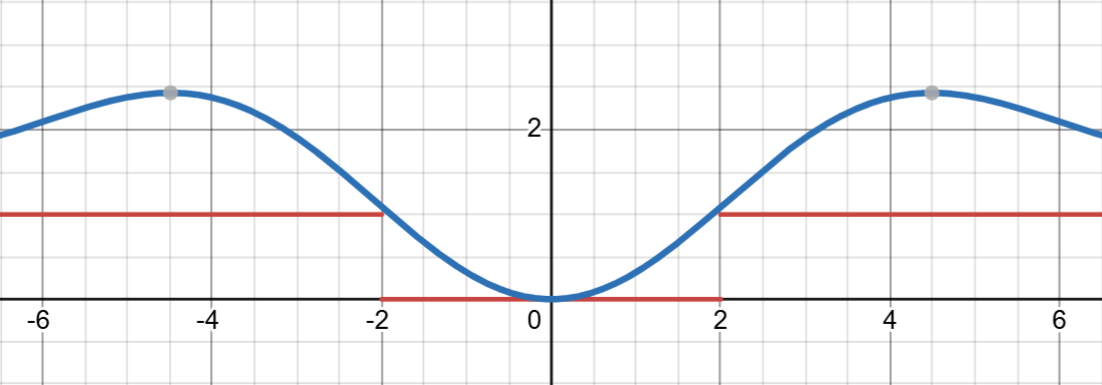
\includegraphics[width=0.82\textwidth]{figures/02-tail-bound-plot.png}
  \caption{$\mathbb I(|x|>2)$ 与 $2(1-\sin x/x)$ 的比较（Desmos 绘制）}
  \label{fig:ch2:tail-bound}
\end{figure}


这个不等式建立了``尾部概率''与``特征函数实部''之间的桥梁：将 $x$ 替换为随机变量 $X_n$，取期望并利用 Fubini 定理交换期望与积分得：\[P(|X_n| > 2/\delta) \le \frac{1}{\delta} \int_{-\delta}^{\delta} \mathbb{E}[1 - \cos(t X_n)] \mathrm{d}t = \frac{1}{\delta} \int_{-\delta}^{\delta} \operatorname{Re}\big(1 - \mathbb{E} [e^{i t X_n}]\big)  \mathrm{d}t\]
由假设，对每个 $t$，$\mathbb{E} [e^{i t X_n}] \to \phi(t)$，故上式中的被积函数逐点收敛到 $\operatorname{Re}(1 - \phi(t))$；利用控制收敛定理，当 $n \to \infty$ 时，\[\frac{1}{\delta} \int_{-\delta}^{\delta} \operatorname{Re}\big(1 -  \mathbb{E}[ e^{i t X_n}]\big)  \mathrm{d}t \to \frac{1}{\delta} \int_{-\delta}^{\delta} \operatorname{Re}(1 - \phi(t)) \mathrm{d}t\]
由于 $\phi$ 在零点连续，对任意 $\epsilon > 0$，存在 $\delta > 0$ 使得当 $|t| < \delta$ 时，$|1 - \phi(t)| < \epsilon$，从而 $\operatorname{Re}(1 - \phi(t)) \le |1 - \phi(t)| < \epsilon$。有\[\frac{1}{\delta} \int_{-\delta}^{\delta} \operatorname{Re}(1 - \phi(t))  \mathrm{d}t \le \frac{1}{\delta} \cdot 2\delta \epsilon = 2\epsilon\]
至此，我们表明了：对充分大的 $n$，\[P(|X_n| > 2/\delta) \le 2\epsilon\]
取 $M = 2/\delta$，则对任意 $\epsilon > 0$，存在 $M$ 和 $N$ 使得当 $n \ge N$ 时，$P(|X_n| > M) < 2\epsilon$ ，即得整个序列 $\{X_n\}$ 是胎紧的。

由 $\{X_n\}$ 胎紧，由 Prohorov 定理，取其任意子列，都可以在其中再抽出一个子列依分布收敛到某随机向量 $Y$。对该收敛子序列，其特征函数收敛到 $\phi$，故 $Y$ 的特征函数为 $\phi$ ，而特征函数唯一确定分布，因此所有可能的（弱收敛意义上的）极限点都有相同的分布，即整个序列 $\{X_n\}$ 只有唯一的极限点。这个推理足够表明 $X_n$ 本身依分布收敛到该极限------否则的话存在子列不收敛，矛盾！记该极限为 $X$，则 $X_n\overset{\rm d}\to X$ 且 $X$ 的特征函数为 $\phi$。

\end{proof}

值得一提的是，定理的必要性里，``逐点收敛''可以有加强的结论，

\begin{theorem*}

设 $X_n,X$ 是随机变量， $\phi_n,\phi$ 分别是其特征函数，若 $X_n\overset{\rm d}\to X$，那么 $\phi_n(t)\to \phi(t)$ 内闭一致收敛。

\end{theorem*}

\begin{proof}[证明概述]
Portmanteau 定理告诉我们 $\limsup\limits_{n\to \infty}P(|X_n|>M)\le P(|X|>M)$。因此，对任意 $t$ 和 $h$，
\[
\begin{aligned}
|\phi_n(t+h)-\phi_n(t)|
&\le\int_{\mathbb R}|e^{ihx}-1|\mathrm{d}F_n(x)\\
&\le \int_{|x|\le M}|hx|\mathrm{d}F_n(x)
 +2\int_{|x|>M}\mathrm{d}F_n(x)\\
&\le |h|M+2\int_{|x|>M}\mathrm{d}F(x)+\epsilon.
\end{aligned}
\]
上式对任意给定的 $\epsilon>0$、合适的 $M$ 以及足够大的 $n$ 成立。这证明了 $\{\phi_n\}$ 等度连续。剩下只需要在紧集上用经典的``$3\epsilon$''证明即可。
% ，例如，可参考文章 \url{https://zhuanlan.zhihu.com/p/347240346} 的定理 25。
\end{proof}

我们举两个简单的例子，以表 Lévy 连续定理是多么好用，

\begin{example}[Poisson 分布的中心极限定理]\label{ex:ch2:poisson-clt}
设随机变量 $X_1, \ldots, X_n$ 独立同分布于 $\operatorname{Poisson}(\lambda)$，其中 $\lambda > 0$ 固定，则它们的特征函数为 $\phi_X(t) = e^{\lambda(e^{it} - 1)}$ 。记样本均值 $\bar{X} = n^{-1}\sum_{i=1}^n X_i$，则标准化随机变量 $\frac{\bar{X} - \lambda}{\sqrt{\lambda/n}}$ 的特征函数为\[\begin{aligned} \phi_{\frac{\bar{X} - \lambda}{\sqrt{\lambda/n}}}(t) &= e^{-it\sqrt{n\lambda}} \phi_{\bar{X}}\!\left(\frac{t}{\sqrt{\lambda/n}}\right) = e^{-it\sqrt{n\lambda}} \left(\phi_X\!\left(\frac{t}{\sqrt{n\lambda}}\right)\right)^n \\ &= e^{-it\sqrt{n\lambda}} \exp\left\{n\lambda\left(e^{it/\sqrt{n\lambda}} - 1\right)\right\} \\ &= \exp\left\{-it\sqrt{n\lambda} + n\lambda\left(\frac{it}{\sqrt{n\lambda}} + \frac{(it)^2}{2n\lambda} + o\!\left(\frac{1}{n\lambda}\right)\right)\right\} \\ &= \exp\left\{-\frac{t^2}{2} + o(1)\right\} \\ &\to e^{-t^2/2},\quad \text{ 当 }n\to\infty \end{aligned}\]
这正是 $\mathcal{N}(0,1)$ 的特征函数！于是 Lévy 连续定理告诉我们\[\frac{\bar{X} - \lambda}{\sqrt{\lambda/n}} \overset{\rm d}\to \mathcal{N}(0,1)\]

\end{example}

\begin{example}[弱大数律]
设随机变量 $Y_1,Y_2,\dots,Y_n$ i.i.d.，其特征函数 $\phi_Y(t)$ 在 0 处可导，且 $\phi_Y'(0)=i\mu$ ，那么
\[
\bar Y=\frac1n\sum_{i=1}^nY_i\overset{p}\to \mu.
\]

我们知道，当极限是常数时，依分布收敛和依概率收敛是等价的（见定理~\ref{thm:ch1:convergence-relations} 的第 (3.) 条），只需证明 $\bar Y\overset{\rm d}\to \mu$ 。而由\[\phi_Y(t) = 1 + t\phi_Y'(0) + o(t), \quad t \to 0\]
有\[\phi_{\bar{Y}}(t) = \left(\phi_Y\!\left(\frac{t}{n}\right)\right)^n = \left(1 + \frac{t}{n}\phi'(0) + o\!\left(\frac{t}{n}\right)\right)^n = \left(1 + \frac{i t \mu}{n} + o\!\left(\frac{1}{n}\right)\right)^n \to e^{i t \mu}\]
依 Lévy 连续定理即得。


在下节中我们会表明，本例的 $\mu$ 正是总体均值。

\end{example}

\section{矩与特征函数}

\subsection{特征函数的展开}

这里请读者回忆 Fourier 变换的一个性质：时域函数的光滑程度直接决定了其频谱在高频区域的衰减速度，即，信号在时间上越平滑，其能量就越集中在低频部分，其高频成分消失得也越快。%可以参考 \href{https://www.zhihu.com/question/64361940}{关于Fourier transform的尾部decay rate的具体性质？}

对偶过来，时域的衰减速度也应该决定了频谱的光滑程度。有结论：若 $x^m f(x)\in L^1$ ，则 $f$ 的 Fourier 变换就是 $m$ 次可微的。

放在概率的语境下，$X$ 的分布对应``时域''，特征函数对应``频域''；应该说： $X$ 分布的尾部越薄， $\phi_X$ 就越光滑。根据 Markov 不等式， $P(|X|>x)\le \frac{\mathbb{E}[|X|^m]}{x^m},\,\forall x>0$ ， $\mathbb{E}[|X|^m]<\infty$ 对应于 $X$ 分布的尾部以至少 $x^{-m}$ 的速率衰减。我们可以用如下引理来描述，

\begin{lemma*}

设对于正整数 $m$ ，随机变量 $X$ 满足 $\mathbb{E}[|X|^m]<\infty$ ，那么其特征函数 $\phi_X$ 是 $m$ 次可导的，且其 $m$ 阶导数为
\[
\phi_X^{(m)}(t)=\mathbb{E}\big[(iX)^me^{itX}\big].
\]

特别地， $\phi_X^{(m)}(0)=\mathbb{E}\big[(iX)^m\big]$ 。

\end{lemma*}

\begin{proof}[证明简述]
利用 Lebesgue 控制收敛定理交换极限与积分，易得 $\phi'_X(t)=\mathbb{E}\big[(iX)e^{itX}\big]$，这个操作可以递推 $m$ 次。
\end{proof}

% \begin{remark}

% \begin{itemize}
% \tightlist
% \item
%   比较详细的证明可见 \href{https://www.zhihu.com/question/1987559971278304504/answer/1987590546710102543}{为什么随机变量的l阶矩存在就可以知道特征函数可求导？ - 知乎}；
% \item
%   这个结论同时告诉我们，对特征函数求 0 处 $m$ 阶导可以计算随机变量的 $m$ 阶矩。
% \end{itemize}
% \end{remark}
  这个结论同时告诉我们，对特征函数求 0 处 $m$ 阶导可以计算随机变量的 $m$ 阶矩。对 $\phi_X$ 在 0 处进行 Taylor 展开，可以得到如下定理：

\begin{theorem}[特征函数的 Taylor 展开]
\label{thm:ch2:characteristic-taylor}

设 $\mathbb{E}[|X|^m]<\infty$ ，则\[ \phi_X(t)=\sum_{j=0}^m\frac{(it)^j}{j!}\mathbb{E}[X^j]+o(|t|^m) \]

\end{theorem}

\begin{remark}

\begin{itemize}
\tightlist
\item
  由 Taylor 公式的 Lagrange 型余项，定理~\ref{thm:ch2:characteristic-taylor} 也可以写成：
  \[  \phi_X(t)=\sum_{j=0}^{m-1}\frac{(it)^j}{j!}\mathbb{E}[X^j]+\frac{\lambda |t|^m}{m!}\mathbb{E}[|X|^m],
  \]  其中复数 $|\lambda|\le 1$ 。
\item
  定理~\ref{thm:ch2:characteristic-taylor} 的余项可以由如下不等式控制：
  \[  \left|e^{ix}-\sum_{m=0}^n\frac{(ix)^m}{m!}\right|\leq\min\left(\frac{|x|^{n+1}}{(n+1)!},\frac{2|x|^n}{n!}\right).
  \]  见 \cite{durrett2010}, Lemma 3.3.7。因此
  \[  \left| \phi_X(t) - \sum_{j=0}^m \frac{(it)^j}{j!}\mathbb{E}[X^j] \right| \leq \mathbb{E}\left[ \left| e^{itX} - \sum_{j=0}^m \frac{(itX)^j}{j!} \right| \right] \leq \mathbb{E}\left[ \min\left\{ \frac{|tX|^{m+1}}{(m+1)!}, \frac{2|tX|^m}{m!} \right\} \right].
  \]\end{itemize}
\end{remark}

\subsection{中心极限定理}

仿照例~\ref{ex:ch2:poisson-clt}，我们可以证明一般的中心极限定理：

\begin{example}[中心极限定理]\label{ex:ch2:clt}
设 $X_1, \ldots, X_n$ 是 $\mathbb R$ 上 i.i.d. 的随机变量，有均值 $\mathbb{E}[X_1]=\mu$ 和方差 $\mathbb{E}[(X_1-\mu)^2]=\sigma^2$，其中 $-\infty<\mu<\infty$、$0<\sigma^2<\infty$，则\[\frac{\bar{X} - \mu}{\sqrt{\sigma^2/n}} \xrightarrow{\rm d} \mathcal{N}(0,1)\]
\begin{proof}

将 $X_1,X_2,\dots$ 中心化后的特征函数记为 $\phi_{X-\mu}$，则当 $n\to\infty$，\[\phi_{ \frac{\bar{X} - \mu}{\sqrt{\sigma^2/n}} }(t) = \left(\phi_{X-\mu}\!\left(\frac{t}{\sigma\sqrt{n}}\right)\right)^n = \left(1 - \frac{1}{2}\left(\frac{t}{\sigma\sqrt{n}}\right)^2 \sigma^2 + o\!\left(\frac{t^2}{\sigma^2 n}\right)\right)^n \to e^{-t^2/2}.\]依 Lévy 连续定理即得。

\end{proof}

例~\ref{ex:ch2:clt} 的这个结论也可以写作 $\frac{1}{\sqrt n}\sum_{j=1}^n(X_i-\mu)\overset{\rm d}\to \mathcal{N}(0,\sigma^2)$ 。

\end{example}

\begin{theorem}[Cramér--Wold 定理]\label{thm:ch2:cramer-wold}

设 $\{X_n\}_{n=1}^\infty$ 是一列 $\mathbb R^k$ 上的随机向量，那么\[X_n\overset{\rm d}\to X\ \iff \ c^\top X_n\overset{\rm d}\to c^\top X,\enspace \forall c\in\mathbb R^k\]
即，高维随机向量的依分布收敛等价于其任意方向上的``投影''或者说``边际 (marginal)''的依分布收敛。

\end{theorem}

\begin{proof}

`` $\Longrightarrow$ ''根据连续映射定理是显然的，只需证明`` $\Longleftarrow$ ''。设 $X_n=(X_{n1},\dots,X_{nk})^\top$ 、 $X=(X_1,\dots,X_k)^\top$ ，二者的特征函数分别为 $\phi_n$ 和 $\phi$ 。对于任意的 $c=(c_1,\dots,c_k)^\top\in\mathbb R^k$ ，由假设，\[c_1X_{n1}+\cdots+c_kX_{nk}\overset{\rm d}\to c_1X_1+\cdots +c_kX_k,\quad \text{当 }n\to\infty\]
根据 Lévy 连续定理，上式等价于特征函数的逐点收敛：\[\mathbb{E}\left[e^{it(c_1X_{n1}+\cdots+c_kX_{nk})}\right]\to \mathbb{E}\left[e^{it(c_1X_{1}+\cdots+c_kX_{k})}\right]\]
亦即，
\[
\phi_n(tc_1,tc_2,\dots,tc_n)\to \phi(tc_1,tc_2,\dots,tc_n).
\]

对任意 $t\in\mathbb R$ 成立，取 $t=1$ 即可看出 $\phi_n(c)\to \phi(c),\,\forall c\in\mathbb R^k$ ，从而 $X_n\overset{\rm d}\to X$ 。

\end{proof}

\begin{remark}

\begin{itemize}
\tightlist
\item
  给该定理一个引用出处：\cite{serfling1980} 的 p.18。
\item
  特别地，要证明 $X_n$ 依分布收敛于正态分布，只需要证明对任意的 $t$ 有$t^\top X_n$ 依分布收敛于正态分布；这是因为 $X$ 是多维正态分布当且仅当其每个边际 $t^\top X$ 都是一维正态分布 (e.g., 见 \cite{vershynin2018} 的 Exercise 3.3.4)
\end{itemize}
\end{remark}

\begin{example}[高维中心极限定理]
设 $Y_1,Y_2,\dots,Y_n$ 是 $\mathbb R^k$ 上的 i.i.d. 随机向量，有均值向量 $\mathbb{E}[Y_1]=\mu$ 和协方差矩阵 $\mathbb{E}[(Y_1-\mu)(Y_1-\mu)^\top]=\Sigma$，则 $\frac1{\sqrt n}\sum_{j=1}^n(Y_j-\mu)=\sqrt n(\bar Y-\mu)\overset{\rm d}\to \mathcal{N}(0,\Sigma)$。

\begin{proof}
用 Cramér--Wold 定理化为一维情形。注意到 $t^\top Y_1-t^\top \mu$、$t^\top Y_2-t^\top \mu$、\ldots{} 是 i.i.d. 的、均值为 0、方差为 $t^\top\Sigma t$ 的随机变量，用例~\ref{ex:ch2:clt} 结论，$t^\top\left(\frac1{\sqrt n}\sum_{j=1}^n(Y_j-\mu)\right)=\frac1{\sqrt n}\sum_{j=1}^n(t^\top Y_j-t^\top \mu)\overset{\rm d}\to \mathcal{N}(0,t^\top\Sigma t)$。
\end{proof}

\end{example}

\subsection{矩问题}

一个自然的问题是：既然特征函数完全决定了分布的矩，那么，仅通过分布的矩能否反过来确定分布？

答案是否定的，我们这里仅简略介绍一下。它被称作``\textbf{\emph{矩问题}} (moment problem)''。一个反例 (来自 \cite{heyde1963}) 是对数正态分布，其密度为 $f_0(x)=(2\pi)^{-1/2}x^{-1}e^{-(\log x)^2/2}$ ，以及一个``扰动分布''，其密度为 $f_a(x)=f(x)(1+a\sin(2\pi\log x))$ ，二者拥有相同的各阶原点矩。

记 $\alpha_m:=\mathbb{E}[X^m]$ 为原点矩，若如下的``\textbf{\emph{Carleman 条件}}''成立：\[ \sum_{m=1}^\infty \alpha_{2m}^{-\frac1{2m}}=\infty \]则 $\{\alpha_m\}$ 唯一确定 $X$ 的分布。

直觉上可以理解为，如果分布尾部较厚， $\alpha_{2m}$ 就会增长得很快，那么 $\alpha_{2m}^{-\frac1{2m}}$ 下降得也很快，其求和就会更可能收敛，分布的``唯一性''越弱，导致不同的分布可以拥有完全相同的一组矩；反过来，如果分布尾部较薄， $\alpha_{2m}$ 的增长、以及 $\alpha_{2m}^{-\frac1{2m}}$ 的下降也都会放慢，求和才更偏向于发散，分布的``唯一性''就越强。

Carleman 条件的证明依赖于 Denjoy--Carleman 关于实值函数拟解析性（quasi-analyticity）的定理，不再赘述。
% ，可参考这篇文章的定理11：
% \href{https://zhuanlan.zhihu.com/p/1986628306896962819}{谈概率分布的收敛}
关于矩问题，亦可参阅 \cite{durrett2010} 的 §3.3.6，或者更深入讨论的文献 \cite{schmudgen2017}。

\section{Edgeworth 展开}

中心极限定理告诉我们 $\sqrt{n}(\bar X-\mu)/\sigma$ 依分布收敛于标准正态分布，但这个收敛有多快？对于给定的 $n$ ，近似的误差有多大？以及能否通过修正项提高精度？Edgeworth 展开正是这样一种工具：它将标准化和的分布渐近展开为 $\Phi(x)$ 加上若干修正项，这些修正项由 $X$ 的高阶矩（偏度、峰度等）决定。

对随机变量 $X$ ，我们记其 $m$ 阶原点矩为 $\alpha_m=\mathbb{E}[X^m]$ （特别地， $\alpha_1=\mu$ ），其 $m$ 阶中心矩为 $\mu_m:=\mathbb{E}[(X-\mu)^m]$ （特别地， $\mu_1=0$ 、 $\mu_2=\sigma^2$ ）。$\Phi,\varphi$ 分别是标准正态分布 $\mathcal N(0,1)$ 的分布函数和密度函数。

若对 $m=1,2,\dots$ ， $\mathbb R$ 上随机变量 $X$ 满足 $\mathbb{E}[|X|^m]<\infty$ ，那么根据定理~\ref{thm:ch2:characteristic-taylor}，
\[
\phi_{X-\mu}(t) = 1 + \frac{1}{2}(it)^2\mu_2 +\frac{1}{6}(it)^3 \mu_3 +\cdots + \frac{1}{m!} (it)^m\mu_m + o(|t|^m).
\]

于是，若 $X_1,\dots,X_n$ i.i.d.与 $X$ 同分布，则\[\phi_{\frac{\bar{X}-\mu}{\sqrt{\sigma^2/n}}}(t) = \left(\phi_{X-\mu}\!\left(\frac{t}{\sigma\sqrt{n}}\right)\right)^n = \left(1 - \frac{t^2}{2n} - \frac{i t^3}{6 n^{3/2}} \frac{\mu_3}{\sigma^3} + \frac{t^4}{24 n^2} \frac{\mu_4}{\sigma^4} + \cdots\right)^n.\]
看起来要展开这个式子似乎有些麻烦？

我们想到：可以用对数来将幂化作求和形式。这是一个非常简单直接的技巧：如果 $X$ 和 $Y$ 是独立的随机变量，它们的特征函数相乘 $\phi_{X+Y}(t) = \phi_X(t)\phi_Y(t)$；一旦取了对数，乘法就变成了加法：$\log \phi_{X+Y}(t) = \log \phi_X(t) + \log \phi_Y(t)$。

定义如下概念：对随机变量 $X$ ，称 $\log \phi_X(t)=\log\mathbb{E}[e^{itX}]$ 为其\textbf{\emph{累积生成函数}} (cumulant generating function, CGF)，其 Taylor 展开 \[ \log \phi_X(t)=\sum_{j=1}^\infty \kappa_j\frac{(it)^j}{j!} \]中的各次数 $\kappa_1,\kappa_2,\dots$ 则称作\textbf{\emph{累积量}} (cumulant)。累积量和矩非常类似，也能够提供和矩一样的信息，不难算出：

\begin{itemize}
\tightlist
\item
  $\kappa_1=\frac{{\rm d}\log \phi_X}{\mathrm{d}t}(0)=\frac{\phi'_X(0)}{\phi_X(0)}=\mathbb{E}[X]=\alpha_1$ ;
\item
  $\kappa_2=\frac{{\rm d}^2\log \phi_X}{\mathrm{d}t^2}(0)=\frac{\phi''_X(0)\phi(0)-(\phi'(0))^2}{(\phi_X(0))^2}=\mathbb{E}[X^2]-(\mathbb{E}[X])^2=\alpha_2-\alpha_1^2=\mu_2$ ;
\item
  $\kappa_3=\frac{{\rm d}^3\log\phi_X}{\mathrm{d}t^3}=\alpha_3-3\alpha_2\alpha_1+2\alpha_1^3=\mu_3$ ;
\item
  $\kappa_4=\frac{{\rm d}^4\log \phi_X}{\mathrm{d}t^4}(0)=\alpha_4-4\alpha_3\alpha_1-3\alpha_2^2+12\alpha_2\alpha_1^2-6\alpha_1^4=\mu_4-3\mu_2^2$ ;
\item
  \ldots{}
\end{itemize}

按此继续，例如 $\kappa_{10}$ 可以写成多达 41 项相加。

对于归一化的随机变量 $Y=\frac{X-\mu}{\sigma}$ ，它的前四个累积量是 $\kappa_1=0$ 、 $\kappa_2=1$ 、 $\kappa_3=\frac{\mathbb{E}[(X-\mu)^3]}{\sigma^3}$ 称作 $X$ 的\textbf{\emph{偏度}} (Skewness)、 $\kappa_4=\frac{\mathbb{E}[(X-\mu)^4]}{\sigma^4}-3$ 称作 $X$ 的\textbf{\emph{峰度}} (Kurtosis)。于是\[ \phi_Y(t) = \exp \left\{ \sum_{j = 1}^\infty \frac{(it)^j}{j!} \kappa_j \right\} = \exp \left\{ -\frac{t^2}{2} + \sum_{j = 3}^\infty \frac{(it)^j}{j!} \kappa_j \right\} \]从而，若 $X_1,\dots,X_n$ i.i.d.与 $X$ 同分布，记 $S_n:=\frac{\bar{X}-\mu}{\sqrt{\sigma^2/n}}$ ，则有\[\begin{aligned} \phi_{S_n}(t) &= \left(\phi_Y\left(\frac{t}{\sqrt{n}}\right)\right)^n \\ &= \exp\left\{ -\frac{t^2}{2} + \sum_{j = 3}^\infty \kappa_j \frac{(it)^j}{j!} n^{-\frac{j-2}{2}} \right\} \\ &=e^{-\frac{t^2}{2}}\left(1+\sum_{m=1}^\infty\frac1{m!}\left(\sum_{j=3}^\infty\kappa_j \frac{(it)^j}{j!} n^{-\frac{j-2}{2}} \right)^m\right)\\ &= e^{-\frac{t^2}{2}} \left( 1 + \sum_{j = 1}^\infty n^{-\frac{j}{2}} r_j(it)\right) \end{aligned}\]
其中 $r_j$ 是次数为 $3j$ 的实系数多项式，依赖于 $\kappa_3,\dots,\kappa_{j+2}$ 但不依赖于 $n$ ；如

\begin{itemize}
\tightlist
\item
  $r_1(u)=\frac16\kappa_3u^3$ ;
\item
  $r_2(u)=\frac1{24}\kappa_4 u^4+\frac1{72}\kappa_3^2u^6$ ;
\item
  \ldots{}
\end{itemize}

至此，我们得到了这样的结论

\begin{equation}
\label{eq:ch2:tag-4}
\phi_{S_n}(t)=e^{-\frac{t^2}2}\left(1+n^{-1/2}r_1(it)+n^{-1}r_2(it)+\cdots++n^{-j/2}r_j(it)+\cdots\right)
\end{equation}

上面的第一项正是标准正态分布的特征函数！对比 \[ \phi_{S_n}(t) = \int_{-\infty}^\infty e^{itx}\,\mathrm dP(S_n \leq x), \quad e^{-t^2/2} = \int_{-\infty}^\infty e^{itx}\,\mathrm d\Phi(x) \]则 式~\eqref{eq:ch2:tag-4}向我们传达了一个信息：

\begin{equation}
\label{eq:ch2:tag-5}
P(S_n\le x)=\Phi(x)+n^{-1/2}R_1(x)+n^{-1}R_2(x)+\cdots+n^{-j/2 }R_j(x)+\cdots
\end{equation}

其中 $R_j(x)$ 是一个 Fourier-Stieltjes 变换是 $e^{-\frac{t^2}2}r_j(it)$ 的函数，亦即，\[\int_{\mathbb R}e^{itx}\mathrm{d}R_j(x)=e^{-\frac{t^2}2}r_j(it)\]
下一步，我们的目标就变成了确定 $R_j$ 。由分部积分，\[\begin{aligned}  e^{-t^2/2} &= \int_{-\infty}^\infty  e^{itx}\,\mathrm d\Phi(x)\\ & =(-it)^{-1}\int_{-\infty}^{\infty}e^{itx}\mathrm d\Phi'(x) \\   & =(-it)^{-2}\int_{-\infty}^{\infty}e^{itx}\mathrm d\Phi''(x) \\   \vdots\\   & =-(-it)^{-j}\int_{-\infty}^{\infty}e^{itx}\mathrm d\Phi^{(j)}(x) \end{aligned}\]
可以看出
\[
\int_{-\infty}^\infty e^{itx}\mathrm{d}((-D)^j\Phi(x))
=(it)^je^{-t^2/2},
\]
其中 $D=\frac{\mathrm d}{\mathrm dx}$ 是微分算子。我们把多项式 $r_j$ 作用在 $-D$ 上，得到 $r_j(-D)$ （这本身仍然是一个微分算子），于是上式表明\[\int_{-\infty}^\infty e^{itx}\mathrm{d}(r_j(-D)\Phi(x))=r_j(it)e^{-\frac{t^2}2}\]
我们想找的 $R_j$ 就此现身！由式~\eqref{eq:ch2:tag-5} 立即推出 $R_j(x)=r_j\left(-D\right)\Phi(x)$

此外，Hermite 多项式定义为
\[
\mathrm{He}_n(x):=(-1)^ne^{x^2/2}\frac{\mathrm{d}^n}{\mathrm{d}x^n}e^{-x^2/2}.
\]
这是一个 $n$ 次的实系数首一多项式：

\begin{itemize}
\tightlist
\item
  $\mathrm{He}_0(x)=1$ ;
\item
  $\mathrm{He}_1(x)=x$ ;
\item
  $\mathrm{He}_2(x)=x^2-1$ ;
\item
  $\mathrm{He}_3(x)=x^3-3x$ ;
\item
  $\mathrm{He}_4(x)=x^4-6x^2+3$ ;
\item
  $\mathrm{He}_5(x)=x^5-10x^3+15x$ ;
\item
  \ldots{}
\end{itemize}

并且满足 $(-D)^j\varphi(x)=\mathrm{He}_{j}(x)\varphi(x)$；那么当 $j\ge 1$ 时，
\[
(-D)^j\Phi(x)=-\mathrm{He}_{j-1}(x)\varphi(x).
\]
据此可以具体算出 $R_j(x)$，

\begin{itemize}
\tightlist
\item
  $R_1(x)=r_1(-D)\Phi(x)=\frac16\kappa_3(-D)^3\Phi(x)=-\frac16\kappa_3(x^2-1)\varphi(x)$ ;
\item
  \[
  \begin{aligned}
  R_2(x)&=r_2(-D)\Phi(x)\\
  &=\left(\frac1{24}\kappa_4 (-D)^4\Phi(x)+\frac1{72}\kappa_3^2(-D)^6\Phi(x)\right)\\
  &=-\left(\frac1{24}\kappa_4(x^3-3x)+\frac1{72}\kappa_3^2(x^5-10x^3+15x)\right)\varphi(x).
  \end{aligned}
  \]
\item
  \ldots{}
\end{itemize}

一般地，可以写作 $R_j(x)=p_j(x)\varphi(x)$ ，其中 $p_j$ 是一个 $3j-1$ 次多项式。 式~\eqref{eq:ch2:tag-5}便可写作\[P(S_n\le x)=\Phi(x)+n^{-1/2}p_1(x)\varphi(x)+n^{-1}p_2(x)\varphi(x)+\cdots+n^{-j/2 }p_j(x)\varphi(x)+\cdots\]
这就是 \textbf{\emph{Edgeworth 展开 }} (Edgeworth expansion)。

Edgeworth 展开往往只有\emph{渐近展开}的意义，即其描述的是 $n\to\infty$ 时的行为。使用 Edgeworth 展开时，最常用到的一个条件称作 \textbf{\emph{Cramér 条件 }}：如果 $X$ 满足 $\mathbb{E}[|X|^{j+2}]<\infty$ 且 $\limsup\limits_{|t|\to\infty}|\phi_X(t)|<1$ ，则可以将 Edgeworth 展开写到第 $j+1$ 项：\[P(S_n\le x)=\Phi(x)+n^{-1/2}p_1(x)\varphi(x)+n^{-1}p_2(x)\varphi(x)+\cdots+n^{-j/2 }p_j(x)\varphi(x)+o(n^{-j/2}),\quad \text{ 当 }n\to\infty\]
它的重要意义在于\emph{提供了中心极限定理的修正 }，并且，如果能够获得总体分布的三阶或更高阶矩的信息，则可以获得更高阶的修正项，因此，它常常用于提高统计量的收敛速度或提升统计推断的准确性。例如，Bootstrap 的正确性和 Edgeworth 展开有很大的关系，经典著作 \cite{hall1992} 就详细介绍了此事。

\begin{example}[指数分布的 Edgeworth 展开]
这个例子来自于 \href{https://gregorkb.github.io/nonparm/edgeworthplay.html}{Karl Gregory}。设 $X_1,\dots,X_n$ i.i.d. 服从指数分布 $\mathrm{Exp}(\lambda)$ ，那么，总体均值为 $\mathbb{E}[X_1]=1/\lambda$ 、方差 $\mathrm{Var}[X_1]=1/\lambda^2$ ，峰度和偏度分别是 $\kappa_3=2$ 和 $\kappa_4=6$。记
\[
S_n:=\sqrt n\frac{\bar{X}-1/\lambda}{1/\lambda},
\]
则它的分布为 $\mathrm{Ga}(n,n^{1/2})-\sqrt n$。考虑用 Edgeworth 展开近似这个分布：

\begin{itemize}
\tightlist
\item
  0 阶： $\Phi(x)$ ；
\item
  1 阶： $\widetilde{F}_{S_n}^{(1)}(x) =\Phi(x) - \frac{1}{3\sqrt{n}} (x^2 - 1) \varphi(x)$ ；
\item
  2 阶： $\widetilde{F}_{S_n}^{(2)}(x) = \widetilde{F}_{S_n}^{(1)}(x) - \frac{1}{n}\left(\frac{1}{4}(x^3 - 3x) + \frac{1}{18} (x^5 - 10x^3 + 15x) \right) \varphi(x)$ 。
\end{itemize}

取 $n=6$ 时的结果如图~\ref{fig:ch2:edgeworth-exponential} 所示：

\begin{figure}[htbp]
  \centering
  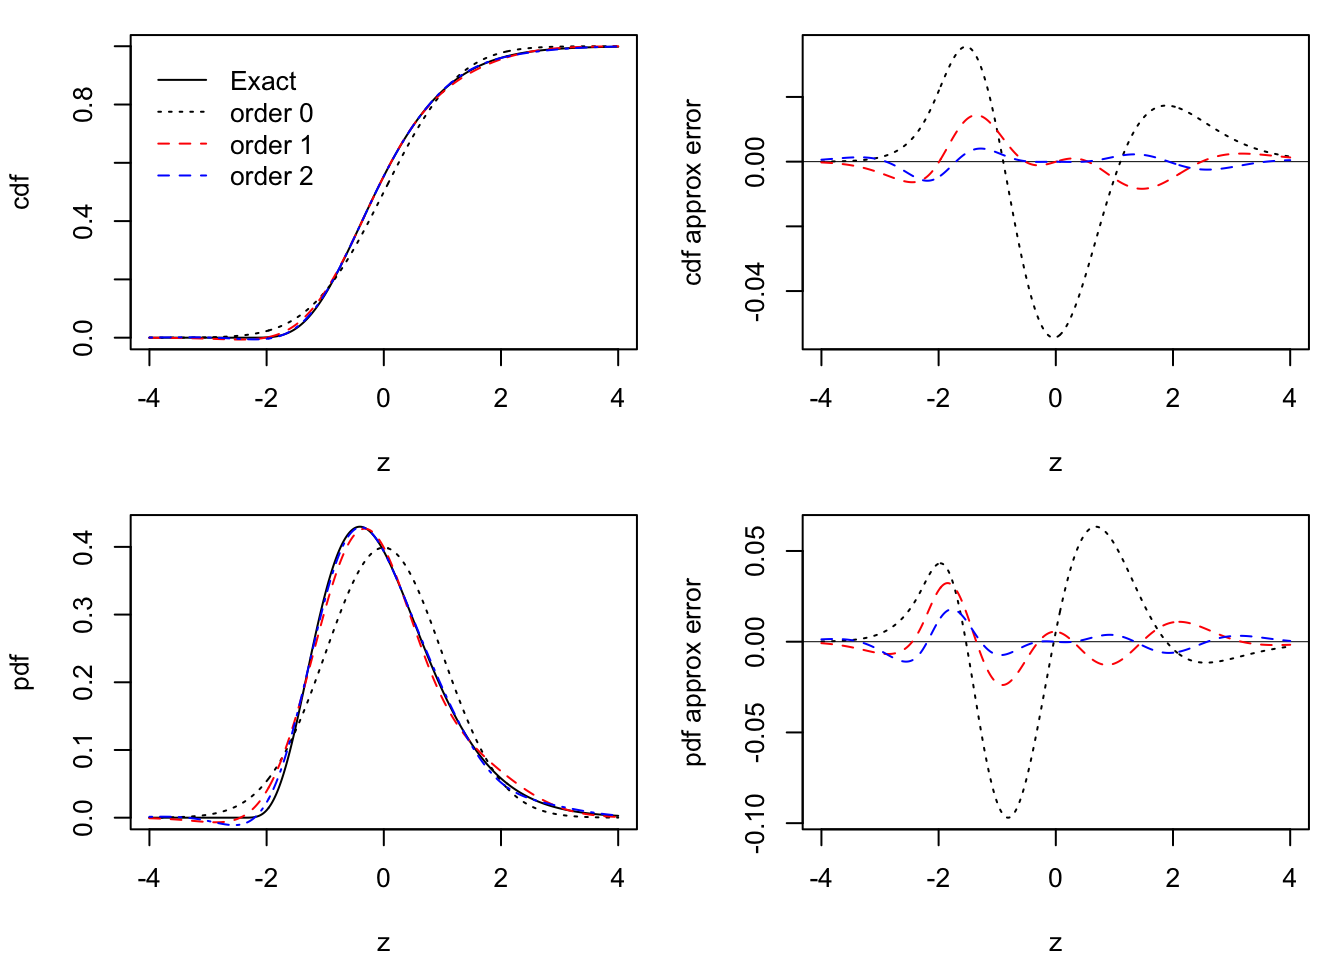
\includegraphics[width=0.88\textwidth]{figures/02-edgeworth-expansion.png}
  \caption{$n=6$ 时指数分布标准化样本均值的 Edgeworth 近似；图片来自 \url{https://gregorkb.github.io/nonparm/edgeworthplay.html}}
  \label{fig:ch2:edgeworth-exponential}
\end{figure}

\end{example}


% Karl Gregory 的博客内容清晰生动、深入浅出，可以去看一看： \url{https://gregorkb.github.io/nonparm/edgeworth.html}、\url{https://gregorkb.github.io/nonparm/edgeworthplay.html}、\url{https://gregorkb.github.io/nonparm/edgeworthmulti.html}、\url{https://gregorkb.github.io/nonparm/edgeworthboot.html}。

Edgeworth 展开解决的是正向问题：``已知分位点 $x$，求更精确的概率分布 $P(S_n \le x)$''。而在实际中，也会遇到需要反向操作的情况：``已知概率 $\alpha$，求更精确的分位数 $x_\alpha$''；这种情况下，将 Edgeworth 展开``反转''，可以得到著名的 \textbf{\emph{Cornish-Fisher 展开}} ，我们会在~\ref{sub:ch11b:cornish-fisher} 中详细说明。

还有要指出的是，读者可能了解``描述中心极限定理的收敛''的另一个结论：\textbf{\emph{Berry-Essen 界}} ， $|F_{S_n}(x)-\Phi(x)|\le \frac{C\mathbb{E}[|X_1-\mu|^3]}{\sigma^3\sqrt n},\quad \forall x\in\mathbb R,\forall n$Berry-Essen 界的优点在于它是一个一致的误差界，但它无法提供中心极限定理的修正信息，是做不到纠偏的。 Edgeworth 展开可以明确将误差分解为 $n^{-1/2}, n^{-1}, \dots$ 项，从而构造出更精确的逼近。

最后，高维情形下 Edgeworth 展开的核心逻辑是不变的，但实际写起来非常非常的繁琐：这需要将累积量 $\kappa_j$ 推广到 $\phi_X(t)$ 在 0 处的多元 Taylor 级数的系数，还要定义高维的 Hermite 多项式。当维数增大时，展开式中的项数会爆炸式增长。由于复杂性，其在实际数据分析中的直接应用不如一维广泛，我们这里不再细述。

\nocite{vandervaart1998,durrett2019}
\chapterreferences
\end{refsection}

\begin{refsection}
\chapter{中心极限定理}\label{ch:central-limit-theorems}
% Generated from: Zhihu/专栏：概率与统计/渐近统计 (3) ：中心极限定理_金鱼马_2026-06-09.md
概率和统计的意义在于描述由大量随机因素影响所表现出来的规律性，因此，研究随机变量和的极限对于搞清楚随机现象的本质有着极其重要的价值。这之中最为重要的结论，莫属中心极限定理 (Central Limit Theorem, CLT)。关于这个定理，大家熟悉的形式一般有下面两种。

\begin{theorem}[De Moivre--Laplace 中心极限定理]
设一列随机变量 $\{X_n\}_{n=1}^\infty$ i.i.d. 服从两点分布
\[
P(X_1=1)=p,\qquad P(X_1=0)=1-p,\qquad 0<p<1.
\]
令 $S_n=\sum_{k=1}^nX_k$，那么
\[
\frac{S_n-np}{\sqrt{np(1-p)}}\overset{\rm d}\longrightarrow\mathcal N(0,1),
\qquad n\to\infty.
\]
\end{theorem}

\begin{theorem}[Lindeberg--L\'evy 中心极限定理]
设一列随机变量 $\{X_n\}_{n=1}^\infty$ i.i.d.，总体均值为
$\mathbb E[X_1]=\mu$，方差为 $\operatorname{Var}[X_1]=\sigma^2<\infty$。
令 $S_n=\sum_{k=1}^nX_k$，那么
\[
\frac{S_n-n\mu}{\sqrt n\sigma}\overset{\rm d}\longrightarrow\mathcal N(0,1),
\qquad n\to\infty.
\]
\end{theorem}

历史上，CLT 理论的发展很大程度得益于 20 世纪 20 年代特征函数的引入。前述结论已经在第~\ref{ch:characteristic-functions}~章中用“特征函数 + L\'evy 连续定理”得到证明。

但在实际应用中，我们经常遇到更一般的情况：
\begin{itemize}
\item 每个 $X_i$ 独立但可能具有不同的分布；
\item 每个 $X_i$ 可能不独立，而是存在某种相依性。
\end{itemize}
这就需要我们寻找更一般的极限定理。

此外，除了减弱随机变量的同分布以及独立性要求，CLT 的研究还有两个方向：讨论向标准正态分布 $\mathcal N(0,1)$ 收敛的问题，以及计算估计收敛的速度（Berry--Esseen 界）等。

本章将证明独立不同分布情况下随机变量组列的两个重要极限定理：Lyapunov CLT 和 Lindeberg--Feller CLT；以及非独立的一种情形：$m$-相依随机变量列的中心极限定理。主要参考 Chung~\cite[第 7 章]{chung2001}。

首先，我们讨论极限理论的一般问题。与其讨论随机变量列，我们在此讨论其“组列”：
\[
\begin{array}{cccc}
X_{11},&X_{12},&\cdots,&X_{1k_1},\\
X_{21},&X_{22},&\cdots,&X_{2k_2},\\
\vdots&\vdots&&\vdots\\
X_{n1},&X_{n2},&\cdots,&X_{nk_n},\\
\vdots&\vdots&&\vdots
\end{array}
\]

\begin{definition*}[独立随机变量组列]
对任意 $n\ge1$，设 $\{X_{n1},X_{n2},\dots,X_{nk_n}\}$ 是概率空间
$(\Omega_n,\mathcal F_n,P_n)$ 上的一组随机变量，满足
$X_{n1},\dots,X_{nk_n}$ 相互独立，且当 $n\to\infty$ 时 $k_n\to\infty$。
则 $\{X_{nj}:1\le j\le k_n\}_{n\ge1}$ 被称作独立随机变量的组列，也叫做“双阵列 (double array)”。本章中涉及的组列都满足独立性，不再反复说明。
\end{definition*}

传统的随机变量列 $\{X_n\}_{n=1}^\infty$ 里，每增加一个 $n$，我们只是在原始序列中多取一个随机变量；这隐含地假定了随机变量的分布是“固定”的：随着 $n$ 增大，我们只是累积更多的样本。然而在组列 $\{X_{nj}:1\le j\le k_n\}_{n\ge1}$ 里，每一行的随机变量个数、分布可以完全不同，因而也更加灵活。传统随机变量列只是组列的一个特例，它可以视作三角组列 $\{X_j:1\le j\le n\}_{n\ge1}$。

我们讨论的目标是形如 $S_n:=\sum_{j=1}^{k_n}X_{nj}$ 的行和，当 $n\to\infty$ 时的极限是什么？收敛于极限分布族中某一给定分布的条件是怎样的？

这里约定符号
\[
\begin{aligned}
\mu_{nj}&:=\mathbb E[X_{nj}],
&\mu_n&:=\sum_{j=1}^{k_n}\mathbb E[X_{nj}]=\sum_{j=1}^{k_n}\mu_{nj},\\
\sigma_{nj}^2&:=\operatorname{Var}[X_{nj}],
&\sigma_n^2&:=\sum_{j=1}^{k_n}\operatorname{Var}[X_{nj}]=\sum_{j=1}^{k_n}\sigma_{nj}^2.
\end{aligned}
\]
在使用这些符号时总假定其为有限值。

\section{Lyapunov 中心极限定理}

\subsection{Lyapunov 条件和 Lyapunov CLT}

\begin{theorem}[Lyapunov CLT]

\label{thm:ch3:3-1}

对独立随机变量组列$\{X_{nj} : 1 \leq j \leq k_n\}_{n \geq 1}$，记 $\Gamma_n := \sum_{j=1}^{k_n} \mathbb{E}\big[|X_{nj} - \mu_{nj}|^3\big]$，且该值对每个 $n$ 都是有限的。那么，若下述的 \textbf{\emph{Lyapunov 条件 }} 成立：
\[\frac{\Gamma_n}{\sigma_n^3} = \frac{1}{\sigma_n^3} \sum_{j=1}^{k_n} \mathbb{E}\big[|X_{nj} - \mu_{nj}|^3\big] \to 0 \quad \text{当 } n \to \infty\]
则
\[
\frac{S_n - \mu_n}{\sigma_n} \overset{\rm d}\to\mathcal N(0, 1).
\]

\end{theorem}

\begin{remark}
定理中的 3 阶矩条件其实过强，常数 3 可以换作任意的 $2+\delta$，其中 $\delta>0$。这种情况下的证明也完全类似。
\end{remark}

容易看到，随机变量列 $\{X_j\}_{j=1}^\infty$ 的 CLT 是定理~\ref{thm:ch3:3-1} 的直接推论，或者更直白地，定理~\ref{thm:ch3:3-1} 能直接翻译成随机变量列的形式：设 $\{X_j\}_{j=1}^\infty$ 是一列独立的随机变量，且对诸 $j$ 有 $\mathbb{E}[X_j]=\mu_j$ 、 $\mathrm{Var}[X_j]=\sigma_j^2<\infty$ 、 $\mathbb{E}[|X_j-\mu_j|^3]=\gamma_j<\infty$ 。若下述 Lyapunov 条件成立：
\[
\frac1{\sigma_n^3}\sum_{j=1}^n\gamma_j\to 0,\quad \text{当 } n \to \infty,
\]

那么
\[
\frac{S_n - \mu_n}{\sigma_n} \overset{\rm d}\to \mathcal{N}(0, 1).
\]

Lyapunov CLT 的一个直接推论如下。

\begin{corollary}

\label{cor:ch3:3-2}对独立随机变量组列$\{X_{nj} : 1 \leq j \leq k_n\}_{n \geq 1}$，若 $\left|\frac{X_{nj}}{\sigma_{n}}\right|\le M_{nj}$ a.s.，且 $\lim\limits_{n\to\infty}\max_{1\le j\le k_n}M_{nj}=0$，那么
\[
\frac{S_n-\mu_n}{\sigma_n}\overset{\rm d}\longrightarrow\mathcal N(0,1).
\]

\end{corollary}

\begin{proof}

注意到 $\mathbb{E}[|X_{nj}-\mathbb{E}[X_{nj}]|^3]\le 2M_{nj}\sigma_n\mathbb{E}[|X_{nj}-\mathbb{E}[X_{nj}]|^2]=2M_{nj}\sigma_n\sigma_{nj}^2$ ，因此 \[ \sum_{j=1}^{k_n}\mathbb{E}\big[|X_{nj}-\mathbb{E}[X_{nj}]|^3\big]\le 2\sigma_n\left(\max_{1\le j\le k_n}M_{nj}\right)\sum_{j=1}^{k_n}\sigma_{nj}^2=2\sigma_n^3\max_{1\le j\le k_n}M_{nj} \]故 $\max\limits_{1\le j\le k_n}M_{nj}\to 0$ 成立蕴含 Lyapunov 条件成立。

\end{proof}

该推论会在后文中用于 Lindeberg-Feller CLT 的证明。

接下来我们将使用两种方式证明定理~\ref{thm:ch3:3-1}。

\subsection{准备工作一}

我们知道，与实数情况类似，当复数 $|z|<1$ 时有``Taylor 展开''
\[\log(1+z) = \sum_{n=1}^{\infty} (-1)^{n-1} \frac{z^n}{n}\]
这里 $\log$ 是复对数函数主支。

下面的引理可以视作重要极限 $\lim\limits_{n \to \infty} \left(1 + \tfrac\theta n\right)^n \to e^\theta$ 的推广，在后面能帮助我们``将复杂的乘积转化为相对简单的形式''。

\begin{lemma}

\label{lem:ch3:3-3}

令 $\{ \theta_{nj} : 1 \leq j \leq k_n \}_{n \geq 1}$ 是一个复数的组列，满足当 $n \to \infty$ 时：

\begin{enumerate}
\def\labelenumi{\arabic{enumi}.}
\tightlist
\item
  $\max\limits_{1 \leq j \leq k_n} |\theta_{nj}| \to 0$，
\item
  $\sum\limits_{j=1}^{k_n} |\theta_{nj}| \leq M < \infty$，其中 $M$ 与 $n$ 无关，
\item
  $\sum\limits_{j=1}^{k_n} \theta_{nj} \to \theta$，其中 $\theta$ 是一个有限复数，
\end{enumerate}

则
\[
\prod_{j=1}^{k_n}(1+\theta_{nj})\to e^\theta.
\]

\end{lemma}

\begin{proof}

条件 (1.) 意味着当 $n$ 充分大时有
\[
\max_{1\le j\le k_n}|\theta_{nj}|\le \frac12.
\]
因此，对每个 $j\le k_n$，复数 $1+\theta_{nj}$ 都位于圆盘 $D(1,1/2)$ 内。该圆盘包含于右半平面，既不包含原点，也不与复对数主支的分支切线相交，故可以统一使用上述 Taylor 展开。此时
\[
\begin{aligned}
\left|\log(1+\theta_{nj})-\theta_{nj}\right|
&=\left|\sum_{m\ge2}(-1)^{m-1}\frac{\theta_{nj}^m}{m}\right|\\
&\le \sum_{m\ge2}\frac{|\theta_{nj}|^m}{m}\\
&\le \frac{|\theta_{nj}|^2}{2}
  \sum_{m=2}^{\infty}\left(\frac12\right)^{m-2}\\
&=|\theta_{nj}|^2.
\end{aligned}
\]
当 $\theta_{nj}\ne0$ 时，令
\[
\lambda_{nj}
:=\frac{\log(1+\theta_{nj})-\theta_{nj}}{|\theta_{nj}|^2};
\]
当 $\theta_{nj}=0$ 时，令 $\lambda_{nj}=0$。于是 $|\lambda_{nj}|\le1$，并且
\[
\log(1+\theta_{nj})
=\theta_{nj}+\lambda_{nj}|\theta_{nj}|^2.
\]
因此
\[
\sum_{j=1}^{k_n}\log(1+\theta_{nj})
=\sum_{j=1}^{k_n}\theta_{nj}
+\sum_{j=1}^{k_n}\lambda_{nj}|\theta_{nj}|^2.
\]
\begin{itemize}
\tightlist
\item
  根据条件 (3.)，上式右侧第一项趋于 $\theta$ 。
\item
  根据条件 (1.) 和 (2.)，上式右侧第二项趋于 0，
\end{itemize}
\[\left|\sum_{j = 1}^{k_n}\lambda_{n j}|\theta_{n j}|^{2}\right|\leq \max_{1\leq j\leq k_{n}}|\theta_{n j}|\sum_{j = 1}^{k_{n}}|\theta_{n j}| \leq \max_{1\leq j\leq k_{n}}|\theta_{n j}|M \to 0\]
这就证明了
\[
\sum_{j=1}^{k_n}\log(1+\theta_{nj})\to\theta.
\]
最后，注意这里并不需要使用复对数通常不成立的乘法公式。直接利用指数函数，有
\[
\begin{aligned}
\prod_{j=1}^{k_n}(1+\theta_{nj})
&=\prod_{j=1}^{k_n}\exp\!\bigl(\log(1+\theta_{nj})\bigr)\\
&=\exp\!\left(\sum_{j=1}^{k_n}\log(1+\theta_{nj})\right)
\longrightarrow e^\theta.
\end{aligned}
\]
这便证明了结论。

\end{proof}

第二个引理比较简单：它描述的是随机变量矩的不等关系

\begin{lemma}[Lyapunov 不等式]

\label{lem:ch3:3-4}

设随机变量 $X$ 的 $s$ 阶绝对矩存在， $0<r<s$ ，则有
\[
\bigl(\mathbb{E}[|X|^r]\bigr)^{1/r} \le \bigl(\mathbb{E}[|X|^s]\bigr)^{1/s}.
\]

\end{lemma}

这是 Hölder 不等式的直接推论。


\subsection{证明一：特征函数方法}

\begin{proof}

总的思想是对特征函数用引理~\ref{lem:ch3:3-3}，然后依 Lévy 连续定理完成证明。针对引理~\ref{lem:ch3:3-3} 的三个条件，我们分成三步。

\begin{enumerate}[label=\textbf{第\chinese*步}:, leftmargin=6em]

\item 令 $\gamma_{nj} := \mathbb{E}\big[|X_{nj} - \mu_{nj}|^3\big]$ ，Lyapunov 不等式（引理~\ref{lem:ch3:3-4}）意味着
\[\sigma_{nj} = \left(\mathbb{E}\big[|X_{nj} - \mu_{nj}|^2\big]\right)^{1 / 2}\leq \left(\mathbb{E}\big[|X_{nj} - \mu_{nj}|^3\big]\right)^{1 / 3}=\gamma_{nj}^{1/3}\]
我们有 $\sigma_{nj}^{3} \leq \gamma_{nj}$，从而，
\[\max_{1\leq j\leq k_n}\sigma_{nj}^3\leq \max_{1\leq j\leq k_n}\gamma_{nj}< \Gamma_n\]
同时，注意到 $\sigma_{nj}^{2} = (\sigma_{nj}^{3})^{2 / 3} \leq (\max_{j} \sigma_{nj}^{3})^{2 / 3}$，

\begin{equation}
\label{eq:ch3:tag-2}
\frac{\max_j \sigma_{nj}^2}{\sigma_n^2} \leq \left(\frac{\max_j \sigma_{nj}^3}{\sigma_{n}^3}\right)^{2 / 3} \leq \left(\frac{\Gamma_{n}}{\sigma_{n}^3}\right)^{2 / 3}
\end{equation}

令 $\phi_{nj}$ 为中心化变量 $\frac{X_{nj} - \mu_{nj}}{\sigma_n}$ 的特征函数，由 $\gamma_{nj}$ 是有限的，根据定理~\ref{thm:ch2:characteristic-taylor}，
\[\phi_{nj}(t) = 1 - \frac{\sigma_{nj}^2t^2}{2\sigma_n^2} +\frac{\lambda_{nj}\gamma_{nj}t^3}{6\sigma_n^3}\]
其中 $|\lambda_{nj}|\le 1$ 。于是
\[\begin{aligned} \max_{1\leq j\leq k_n}|\phi_{nj}(t) - 1|&\leq \frac{t^2}{2\sigma_n^2}\underset {1\leq j\leq k_n}{\max}\sigma_{nj}^2 +\frac{t^3}{6\sigma_n^3} \max_{1\leq j\leq k_n}\gamma_{nj}\\ &\leq \frac{t^2}{2}\left(\frac{\Gamma_n}{\sigma_n^3}\right)^{2 / 3} + \frac{t^3}{6}\frac{\Gamma_n}{\sigma_n^3}  \\ &\to 0\end{aligned}\]
第二行不等式用到了式 $(1),(2)$ 中的界，第三行由 Lyapunov 条件给出。

这推导出引理~\ref{lem:ch3:3-3} 的条件 (1.)。

\item 同时，式~\eqref{eq:ch3:tag-2} 表明
\[\sum_{j = 1}^{k_n}|\phi_{nj}(t) - 1|\leq \frac{\sum_j\sigma_{nj}^2t^2}{2\sigma_n^2} +\frac{t^3}{6}\frac{\Gamma_n}{\sigma_n^3} = \frac{t^2}2 +\frac{t^3}{6}\frac{\Gamma_n}{\sigma_n^3}\]
当 $t$ 固定时上式右侧总是有界的，这建立了引理~\ref{lem:ch3:3-3} 的条件 (2.)。

\item 由于

$$\left|\sum_{j = 1}^{k_n}\frac{\lambda_{nj}\gamma_{nj}}{\sigma_n^3}\right|\leq \frac{\Gamma_n}{\sigma_n^3}\to 0$$

式~\eqref{eq:ch3:tag-2} 还能推出 

$$\sum_{j = 1}^{k_n}(\phi_{nj}(t) - 1) = -\frac{t^2}2 +t^3\sum_{j = 1}^{k_n}\frac{\lambda_{nj}\gamma_{nj}}{\sigma_n^3}\rightarrow -\frac{t^2}2$$

这便得到了引理~\ref{lem:ch3:3-3} 的条件 (3.)。

综上，引理~\ref{lem:ch3:3-3} 的条件满足， $\frac{S_n - \mu_n}{\sigma_n }= \sum_{j = 1}^{k_n}\frac{X_{nj} - \mu_{nj}}{\sigma_n}$ 的特征函数满足
\[\prod_{j = 1}^{k_n}\phi_{nj}(t) = \prod_{j = 1}^{k_n}(1 + \phi_{nj}(t) - 1)\rightarrow e^{-t^2 / 2}\]
上式右侧是标准正态分布 $\mathcal N(0,1)$ 的特征函数。根据 Lévy 连续定理， $\frac{S_n - \mu_n}{\sigma_n }\overset{\rm d}\to \mathcal N(0,1)$ 。

\end{enumerate}

\end{proof}

\subsection{准备工作二}

首先回顾一下第一章介绍的 Portmanteau 定理（定理~\ref{thm:ch1:portmanteau}），其中，我们证明了 $X_n\overset{\rm d}\to X$ 等价于对于所有的有界连续函数类 $f$ 有 $\mathbb{E}[f(X_n)]\to \mathbb{E}[f(X)]$ ；这里的 $f$ 称作``测试函数 (test function)''。这里，我们要将``测试函数类''进行缩小，但同时保证弱收敛的等价性。

在 $\mathbb R^k$ 上有如下函数类：

\begin{itemize}
\tightlist
\item
  有界连续函数类为 $C_b$ 。
\item
  一致连续的函数类为 $C_u$ 。
\item
  ``在无穷远处消失 (vanishing at infinity)'' 的连续函数类记作 $C_0$ ；所谓 $f$ ``在无穷远处消失''指的是 $\lim\limits_{|x|\to\infty}f(x)=0$ 。
\item
  有紧支集的连续函数类为 $C_c$ 。
\end{itemize}

容易验证 $C_c\subset C_0\subset C_u\subset C_b$ ，下面的定理表明``测试函数类''可以缩小至 $C_c$ ：

\begin{lemma}

\label{lem:ch3:3-5}设 $\{X_n\},X$ 是 $\mathbb R^k$ 中的随机向量，若对任意 $f\in C_c$ 有 $\mathbb{E}[f(X_n)]\to \mathbb{E}[f(X)]$ ，那么 $X_n\overset{\rm d}\to X$ 。

\end{lemma}

\begin{proof}

对任意 $\epsilon>0$ ，选取 $h\in C_c$ 使得 $0\le h\le 1$ 且 $\mathbb{E}[h(X)]\ge 1-\epsilon$ 。有命题条件知 $\mathbb{E}[h(X_n)]\to\mathbb{E}[h(X)]$ ，因此对足够大的 $n$ ，同样有 $\mathbb{E}[h(X_n)]>1-\epsilon$ 。

我们证明 $X_n\overset{\rm d}\to X$。对任意 $g\in C_b$，不失一般性设 $|g(x)|\le 1$ 对所有 $x$ 成立。由 $g=gh+g(1-h)$ 和 $gh\in C_c$，
\[\begin{aligned} |\mathbb{E}[g(X_n)]-\mathbb{E}[g(X)]|&\le |\mathbb{E}[g(X_n)h(X_n)]-\mathbb{E}[g(X)h(X)]|+\mathbb{E}[|g(X_n)(1-h(X_n))|]+\mathbb{E}[|g(X)(1-h(X))|]\\ &\le |\mathbb{E}[g(X_n)h(X_n)]-\mathbb{E}[g(X)h(X)]|+2\epsilon\\ &\to 2\epsilon,\quad \text{当 }n\to\infty \end{aligned}\]
\end{proof}

从而，依分布收敛的``测试函数''可以选择 $C_c,C_0,C_u,C_b$ 中任意一类。接下来我们再将之拓展到一类新的函数：用 $C_b^\infty$ 代表 $\mathbb R$ 上任意阶可导、且各阶导数均有界的函数，

\begin{lemma}

\label{lem:ch3:3-6}$C_u$ 中的函数可以被 $C_b^\infty$ 中的函数一致逼近；换言之，在一致收敛拓扑下， $C_b^\infty$ 在 $C_u$ 中是稠密的。

\end{lemma}

\begin{proof}

这里需要用到一种称之为``磨光 (Mollification)'' 的技术。我们选用正态分布 $\mathcal{N}(0,\delta^2)$ 的密度函数 $\varphi_\delta=\frac1{\sqrt{2\pi\delta^2}}e^{-\frac{x^2}{2\delta^2}}$ 。给定 $\mathbb R$ 上的一致连续函数 $f$，将之与 $\varphi_\delta$ 进行卷积，得到

$$f_\delta(x):=(f*\varphi_\delta)(x)=\int_{-\infty}^\infty f(x-y)\varphi_\delta(y)\mathrm dy$$

则 $f_\delta$ 是一个光滑函数，相当于把 $f$ ``磨光''了；并且可以看出其任意阶导数有界，因为根据 Hölder 不等式： \[ \big|f^{(k)}_\delta(x)\big|=\left|\int_{-\infty}^\infty f(x-y)\varphi^{(k)}_\delta(y)\mathrm dy\right|\le \|f\|_\infty\left\|\varphi_\delta^{(k)}\right\|_1<\infty \]于是 $f_\delta\in C_b^\infty$ 。对任意的 $\eta>0$ ，
\[\begin{aligned} |f_\delta(x) - f(x)| &= \left| \int_{-\infty}^{\infty} (f(x-y) - f(x)) \varphi_\delta(y) \mathrm dy \right|\\ &\le \int_{-\infty}^{\infty} |f(x-y) - f(x)| \varphi_\delta(y) \mathrm dy\\ &\le \sup_{|y|\le \eta} |f(x-y) - f(x)|+2\|f\|_\infty\int_{|y|>\eta}\varphi_\delta (y)\mathrm{d}y \end{aligned}\]
当 $\eta$ 充分小时，由一致连续性，上式第一项可以充分小；同时，固定 $\eta$ ，当 $\delta\to 0$ 时，根据正态分布尾部性质，上式第二项也可以充分小。综上， $\lim\limits_{\delta\to 0}\|f_\delta -f\|_\infty=0$ 。

\end{proof}

由引理~\ref{lem:ch3:3-5} 和引理~\ref{lem:ch3:3-6} 立即可得以下推论。

\begin{corollary}

\label{cor:ch3:3-7}设 $\{X_n\},X$ 是 $\mathbb R$ 上的随机变量，若对任意 $f\in C_b^\infty$ 有 $\mathbb{E}[f(X_n)]\to \mathbb{E}[f(X)]$ ，那么 $X_n\overset{\rm d}\to X$ 。

\end{corollary}

\subsection{证明二：Telescoping 方法}

\begin{proof}

对组列的每一元素 $X_{nj}$ ，我们赋予一个独立的辅助随机变量 $Y_{nj}\sim \mathcal N(\mu_{nj},\sigma_{nj}^2)$ 服从正态分布。
我们证明：对任意的 $f\in C_b^3$ ，有 
$$\mathbb{E}\left[f\left(\frac{S_n-\mu_n}{\sigma_n}\right)\right]\to \mathbb{E}\left[f\left(\frac{\sum_j Y_{nj}-\mu_n}{\sigma_n}\right)\right]$$
这里 $\mu_n:=\sum_{j=1}^{k_n}\mathbb{E}[X_{nj}],\,\sigma_{n}^2:=\sum_{j=1}^{k_n}\mathrm{Var}[X_{nj}]$ 含义同前。从而，根据推论~\ref{cor:ch3:3-7} 可以立即得到 $\frac{S_n-\mu_n}{\sigma_n}\overset{\rm d}\to \mathcal{N}(0,1)$ 。

不失一般性， 我们设每个均值 $\mu_{nj}=0$ 。固定 $n$ ，对 $j=1,\dots,k_n$，令
\[Z_{nj} :=\sum_{i<j} Y_{ni} + \sum_{i>j} X_{ni}= \begin{cases} X_{n2}+\cdots+X_{n,k_n},&\text{ 若 }j=1\\ Y_{n1}+\cdots+Y_{n,j-1}+X_{n{j+1}}+\cdots+X_{nk_n},&\text{ 若 }2\le j\le k_n-1\\ Y_{n1}+\cdots+Y_{n,k_n-1}&\text{ 若 }j=k_n \end{cases}\]
注意到 $Y_{nj}+Z_{nj}=X_{n,j+1}+Z_{n,j+1}$ ，于是
\begin{equation}
\label{eq:ch3:tag-4}
\begin{aligned} &\mathbb{E}\left[f\left(\frac{X_{n1}+\cdots+X_{nk_n}}{\sigma_n}\right)\right]- \mathbb{E}\left[f\left(\frac{Y_{n1}+\cdots Y_{nk_n}}{\sigma_n}\right)\right]\\ =\;&\mathbb{E}\left[f\left(\frac{X_{n1}+Z_{n1}}{\sigma_n}\right)\right]- \mathbb{E}\left[f\left(\frac{Y_{nk_n}+Z_{nk_n}}{\sigma_n}\right)\right]\\ =\;&\sum_{j=1}^{k_n}\left(\mathbb{E}\left[f\left(\frac{X_{nj}+Z_{nj}}{\sigma_n}\right)\right]- \mathbb{E}\left[f\left(\frac{Y_{nj}+Z_{nj}}{\sigma_n}\right)\right]\right) \end{aligned}
\end{equation}
对每个 $j$ ，将上式中的 $f$ 用 Taylor 展开到 3 阶
\[\begin{aligned} f\left(\frac{X_{nj}+Z_{nj}}{\sigma_n}\right)&=f\left(\frac{Z_{nj}}{\sigma_n}\right)+f'\left(\frac{Z_{nj}}{\sigma_n}\right)\frac{X_{nj}}{\sigma_n}+\frac12f''\left(\frac{Z_{nj}}{\sigma_n}\right)\frac{X_{nj}^2}{\sigma_n^2}+\frac16\lambda_j^{(1)}\frac{X_{nj}^3}{\sigma_n^3}\\  f\left(\frac{X_{nj}+Y_{nj}}{\sigma_n}\right)&=f\left(\frac{Z_{nj}}{\sigma_n}\right)+f'\left(\frac{Z_{nj}}{\sigma_n}\right)\frac{Y_{nj}}{\sigma_n}+\frac12f''\left(\frac{Z_{nj}}{\sigma_n}\right)\frac{Y_{nj}^2}{\sigma_n^2}+\frac16\lambda_j^{(2)}\frac{Y_{nj}^3}{\sigma_n^3}\\ \end{aligned}\]
其中 $\lambda_j^{(i)}\le \|f'''\|_\infty<\infty$ ， $i=1,2$ 。在我们的设定下， $X_{nj}$ 和 $Y_{nj}$ 的一、二阶矩完全相同，因此取期望并作差后，上面展开式的前三项都会消掉，只剩下三阶项。那么：
\[\begin{aligned} \left|\mathbb{E}f\left(\frac{X_{nj}+Z_{nj}}{\sigma_n}\right) - \mathbb{E}f\left(\frac{Y_{nj}+Z_{nj}}{\sigma_n}\right)\right| &=\frac 1{6\sigma_n^3}\Bigl|\mathbb{E}\bigl[\lambda_j^{(1)}X_{nj}^3\bigr]+\mathbb{E}\bigl[\lambda_j^{(2)}Y_{nj}^3\bigr]\Bigr|\\ &\le \frac{M}{6\sigma_n^3}\Bigl( \mathbb{E}[|X_{nj}|^3] + \mathbb{E}[|Y_{nj}|^3] \Bigr)\\ &=\frac{M}{6\sigma_n^3}\left(\gamma_{nj}+\sqrt{\frac{8}{\pi}}\sigma_{nj}^3\right) \end{aligned}\]
其中 $M=\max\big\{|\lambda_j^{(1)}|,|\lambda_j^{(2)}|\big\}$ 。于是式~\eqref{eq:ch3:tag-4} 有上界：
\[\begin{aligned} \left|\mathbb{E}\left[f\left(\frac{\sum_jX_{nj}}{\sigma_n}\right)\right]- \mathbb{E}\left[f\left(\frac{\sum_jY_{nj}}{\sigma_n}\right)\right]\right| &\le \sum_{j=1}^{k_n}\left|\mathbb{E}\left[f\left(\frac{X_{nj}+Z_{nj}}{\sigma_n}\right)\right]- \mathbb{E}\left[f\left(\frac{Y_{nj}+Z_{nj}}{\sigma_n}\right)\right]\right|\\ &\le \frac{M}{6}\left(\frac{\sum_j\gamma_{nj}}{\sigma_n^3}+\sqrt{\frac{8}{\pi}}\frac{\sum_j\sigma_{nj}^3}{\sigma_n^3}\right)\\ &\le \frac{M}{6}\left(1+\sqrt{\frac8\pi}\right)\frac{\Gamma_n}{\sigma_n^3}\\ &\to 0,\quad \text{当 }n\to\infty \end{aligned}\]
第三行用到了 $\sigma_{nj}^{3} \leq \gamma_{nj}$ (Lyapunov 不等式)，最后一行由 Lyapunov 条件得出。

\end{proof}

\begin{remark}
容易看出，证明中最重要的一步就是式~\eqref{eq:ch3:tag-4}，这个式子（所代表的方法）被称作 \textbf{\emph{Lindeberg's Telescoping Method}}。该方法与 Stein 方法和正态分布逼近 (Gaussian approximation procedures) 密切相关。感兴趣的读者可以参阅 \cite{chernozhukov2013}。这种方法不依赖特征函数，因此在某些情形下更具灵活性。
\end{remark}

\section{Lindeberg-Feller 中心极限定理}

在介绍定理内容之前，我们先介绍两个组列的限制条件。

\subsection{无穷小条件}

回顾文首提出的目标：研究形如 $S_n=\sum\limits_{j=1}^{k_n}X_{nj}$ 在 $n\to\infty$ 时的极限分布。我们比较希望这个极限分布代表了 $X_{nk}$ 的总体特征，而非由少数特殊项决定。一个简单的反例是：对每个 $n$ ， $X_{n1}\sim F$ 而 $X_{nj}=0,j=2,3,\dots$ ，则 $S_n=X_{n1}\sim F$ ，这种情况讨论渐近分布没有什么意义。

为此，一个合理的假设条件是当 $n\to\infty$ 时，每一 $X_{nj}$ 对 $S_n$ 的影响都很微小，使得其极限分布是由``集体''贡献的。换言之，诸 $X_{nj}$ 最好是``一致 $o_P(1)$''的。

什么叫做``一致 $o_P(1)$''呢？来看下面的四个式子：

\begin{enumerate}
\def\labelenumi{\arabic{enumi}.}
\tightlist
\item
  $\displaystyle \forall j, \lim_{n \to \infty} P(|X_{nj} - \mu_{nj}| > \epsilon \sigma_n) = 0$；
\item
  $\displaystyle \lim_{n \to \infty} \max_{1 \leq j \leq k_n} P(|X_{nj} - \mu_{nj}| > \epsilon \sigma_n) = 0$；
\item
  $\displaystyle \lim_{n \to \infty} P\left(\max_{1 \leq j \leq k_n} |X_{nj} - \mu_{nj}| > \epsilon \sigma_n\right) = 0$；
\item
  $\displaystyle \lim_{n \to \infty} \sum_{j=1}^{k_n} P(|X_{nj} - \mu_{nj}| > \epsilon \sigma_n) = 0$。
\end{enumerate}

除了 (1.) 代表每个 $X_{nj}-\mu_{nj}$ 各自是 $o_P(1)$ 外，剩下三个都可以叫做``一致 $o_P(1)$''，并且程度逐渐增强：读者可以证明 $(4.)\implies (3.)\implies (2.)\implies (1.)$ 。

\begin{definition*}[无穷小条件]

若组列 $\{X_{nj},1\le j\le k_n\}_{n\ge 1}$ 满足上面的条件 (2.)，即，对任意 $\epsilon>0$ ，
\[
\lim_{n \to \infty} \max_{1 \leq j \leq k_n} P(|X_{nj} - \mu_{nj}| > \epsilon \sigma_n) = 0,
\]

那么称 $X_{nj}$ 满足\textbf{\emph{无穷小条件}} 。该条件描述了组列的每一行一致地有 $X_{nj}-\mu_{nj}\overset{P}\to 0$ 。

\end{definition*}

\begin{remark}
这个概念有很多不同术语。Gnedenko 与 Kolmogorov 一般称之为``无穷小条件 (infinitesimal)''；Loève 的 GTM 44、GTM 45 中称之为``一致渐近可忽略 (uniformly asymptotically negligible, UAN)''；钟开莱使用``holospoudic''；Feller 使用``零阵列 (null array)''。我国文献一般沿用``无穷小条件''，本文亦然。
\end{remark}

下面一个定理描述无穷小条件的等价定义

\begin{lemma}

\label{lem:ch3:3-8}

组列 $\{X_{nj},1\le j\le k_n\}$ 满足无穷小条件，当且仅当对任意 $t\in\mathbb R$ ，

\begin{equation}
\label{eq:ch3:tag-5}
\lim_{n\to\infty}\max_{1\le j\le k_n}|\phi_{nj}(t)-1|=0
\end{equation}

其中 $\phi_{nj}$ 是 $\frac{X_{nj}-\mu_{nj}}{\sigma_{nj}}$ 的特征函数。

\end{lemma}

\begin{proof}

不失一般性，设每个 $\mu_{nj}=0$ 、 $\sigma_{nj}=1$ ，则 $\phi_{nj}$ 便是 $X_{nj}$ 的特征函数。

必要性：对任意 $\epsilon>0$ ，
\[\begin{aligned} |\phi_{nj}(t) - 1| &= \left| \int e^{itx} {\rm d}F_{nj}(x) - 1 \right| \\ &\le \int |e^{itx} - 1| {\rm d}F_{nj}(x)\\ &\le \int_{|x| \le \varepsilon} |itx| {\rm d}F_{nj}(x) + \int_{|x| > \varepsilon} 2  {\rm d}F_{nj}(x)\\ &\le |t| \varepsilon + 2 P(|X_{nj}| > \varepsilon) \end{aligned}\]
其中第三行用到了不等式 $|e^{itu}-1|=\sqrt{1(2-\cos tu)}\le |tu|$ 。上式给出 $\max_j|\phi_{nj}(t)-1|\le 2\max_j P(|X_{nj}|\ge\epsilon)+|t|\epsilon$ ，从而 式~\eqref{eq:ch3:tag-5}得证。

充分性：我们要用到证明 Lévy 连续定理时用过的一个不等式：对任意 $x \in \mathbb{R}$ 和 $\delta > 0$，有如下不等式成立：
\[\mathbb{I}(|\delta x| > 2) \le 2\left(1 - \frac{\sin \delta x}{\delta x}\right) = \frac{1}{\delta} \int_{-\delta}^{\delta} (1 - \cos t x) \mathrm dt = \frac{1}{\delta} \int_{|t|\le \delta} (1 - \cos t x+i\sin tx) \mathrm dt\]
上式两侧取期望，得到

\begin{equation}
\label{eq:ch3:tag-6}
\begin{aligned} P\left(|X_{nj}|\ge\tfrac2\delta\right)\le \frac1\delta\int_{|t|\le\delta}(1-\phi_{nj}(t)){\rm d}t \end{aligned}
\end{equation}

这给出 $\max_jP\left(|X_{nj}|\ge\tfrac2\delta\right)\le \max_j\frac1\delta\int_{|t|\le\delta}|1-\phi_{nj}(t)|{\rm d}t$ ，利用式~\eqref{eq:ch3:tag-5} 和有界收敛定理交换极限与积分，可以得到 $\lim\limits_{n\to\infty}\int_{|t|\le\delta}\max_j|1-\phi_{nj}(t)|{\rm d}t=0$ 。

\end{proof}

\begin{remark}
式~\eqref{eq:ch3:tag-6} 亦见 \cite{athreya2006} 的 Lemma 10.3.2。
\end{remark}

\subsection{Lindeberg 条件}

\begin{definition*}[Lindeberg 条件]

若组列 $\{X_{nj}, 1 \leq j \leq k_n\}_{n \geq 1}$ 满足：对任意 $\epsilon >0$ ，
\[\lim_{n\to\infty}\frac1{\sigma_n^2}\sum_{j=1}^{k_n}\int_{|x-\mu_{nj}|>\epsilon\sigma_n}(x-\mu_{nj})^2\mathrm{d}F_{nj}(x)\to 0\]
则称该组列满足 \textbf{\emph{Lindeberg 条件}} 。

\end{definition*}

直观上，这是说随着 $n$ 增大，$\sigma_n$ 可能会增长，但要求任何一个 $X_{nj}$ 的偏离超过这个增长门槛的部分可以忽略，从而我们可以对其进行截断而不影响 $S_n$ 的一般性质。这也保证了没有少数变量的波动能够主导整个和：

\begin{lemma}

\label{lem:ch3:3-9}

Lindeberg 条件蕴含无穷小条件。

\end{lemma}

\begin{proof}

只需注意到对任意 $\epsilon >0$ ，
\[
P(|X_{nj} - \mu_{nj}|>\epsilon\sigma_n)= \int_{|x - \mu_{nj}| > \epsilon \sigma_n}\mathrm{d}F_{nj}(x) \le \frac1{\epsilon^2\sigma_n^2}\int_{|x - \mu_{nj}| > \epsilon \sigma_n}(x-\mu_{nj})^2\mathrm{d}F_{nj}(x).
\]

\end{proof}

(这个证明的形式有点像 Chebyshev 不等式，只不过是截断的形式。在后文的证明中我们还会用到。)

在实际应用中，Lindeberg 条件中的截断期望很难计算，因此我们常使用一些更强的充分条件；之前的 Lyapunov 条件就是其一。

\begin{lemma}

\label{lem:ch3:3-10}

对组列 $\{X_{nj}:1\le j\le k_n\}_{n\ge 1}$ ，若存在某 $\delta>0$ 使得
\[\lim_{n\to\infty}\frac1{\sigma_n^{2+\delta}}\sum_{j=1}^{k_n}\mathbb{E}\Big[|X_{nj}-\mu_{nj}|^{2+\delta}\Big]=0\]
那么 Lindeberg 条件成立。

\end{lemma}

\begin{proof}
\[\begin{aligned} \int_{|x-\mu_{nj}|>\epsilon\sigma_n}  (x - \mu_{nj})^2 \mathrm{d}F_{nj}(x)  &\le (\epsilon \sigma_n)^{-\delta} \int_{|x - \mu_{nj}| > \epsilon \sigma_n} (x - \mu_{nj})^{2+\delta} {\rm d}F_{nj}(x) \\ &\le (\epsilon \sigma_n)^{-\delta} \mathbb{E}\Big[|X_{nj} - \mu_{nj}|^{2+\delta}\Big] \end{aligned}\]
从而
\[\frac1{\sigma_n^2}\sum_{j=1}^{k_n}\int_{|x-\mu_{nj}|>\epsilon\sigma_n}  (x - \mu_{nj})^2 \mathrm{d}F_{nj}(x) \le \epsilon^{-\delta}\frac{\sum\limits_{j=1}^{k_n}\mathbb{E}\left[|X_{nj}-\mu_{nj}|^{2+\delta}\right]}{\sigma_n^{2+\delta}}\]
\end{proof}

进一步，推论~\ref{cor:ch3:3-2} 中的一致有界条件也可以推出 Lindeberg 条件。这侧面说明 Lindeberg 条件是足够``精简''的。

\subsection{Lindeberg-Feller CLT 的证明}

Lindeberg 条件是中心极限定理成立的充分条件，我们的定理要证明如下充要条件：

\begin{theorem}[Lindeberg--Feller]\label{thm:ch3:lindeberg-feller}

\label{thm:ch3:3-11}

对独立随机变量组列$\{X_{nj} : 1 \leq j \leq k_n\}_{n \geq 1}$，如下两个陈述等价：

\begin{enumerate}
\def\labelenumi{\arabic{enumi}.}
\tightlist
\item
  $\frac{S_n-\mu_n}{\sigma_n}\overset{\rm d}\to \mathcal{N}(0,1)$ ，且组列满足无穷小条件；
\item
  组列满足 Lindeberg 条件。
\end{enumerate}

\end{theorem}

先证明一个简单的引理，

\begin{lemma}

\label{lem:ch3:3-12}

设 $u(m,n)$ 是关于正整数 $m,n$ 的函数，且对每个 $m$ 有 $\lim\limits_{n\to\infty}u(m,n)=0$ ，那么存在一个单调递增序列 $\{m_n\}_{n\ge 1}$ ， $m_n\to\infty$ 使得 $\lim\limits_{n\to\infty}u(m_n,n)=0$ 。

\end{lemma}

\begin{proof}

给定 $m$ ，由 $\lim\limits_{n\to\infty}u(m,n)=0$ 知存在 $N_m$ 使得当 $n\ge N_m$ 时 $u(m,n)\le \tfrac1m$ 。于是我们得到了一个序列 $\{N_m\}_{m\ge 1}$ ，并且可以让其随 $m$ 严格单调递增。现构造 $m_n$ 如下：当 $N_m\le n\le N_{m+1}$ 时，赋 $m_n=m$ ；则，对这些 $n$ 有 $u(m_n,n)\le \tfrac1m$ ；且由于 $N_m$ 严格单调递增趋向于 $\infty$ ， $m_n$ 亦然。

这一对角序列的构造如图~\ref{fig:ch3:diagonal-sequence} 所示。

\begin{figure}[htbp]
  \centering
  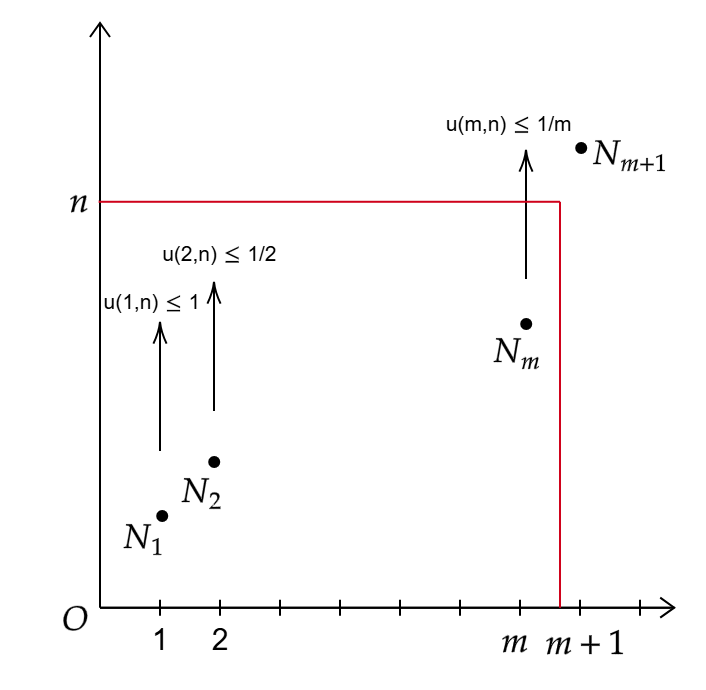
\includegraphics[width=0.58\textwidth]{figures/03-diagonal-sequence.png}
  \caption{对角序列 $m_n$ 的构造示意图（Mathcha 绘制）}
  \label{fig:ch3:diagonal-sequence}
\end{figure}

\end{proof}

下面证明定理~\ref{thm:ch3:3-11}。

\begin{proof}

不失一般性，我们让每个 $X_{nj}$ 的均值 $\mu_{nj}=0$ ，且每行方差和 $\sigma_n^2=1$ ，不然的话可用 $\frac{X_{nj}-\mu_{nj}}{\sigma_{n}}$ 代替 $X_{nj}$ 。

\textbf{\emph((2.) $\Rightarrow$ (1.) )}

由引理~\ref{lem:ch3:3-9}，无穷小条件自动成立，我们只需证明 $S_n\overset{\rm d}\to \mathcal N(0,1)$ 。

这里要用到``截断''的思想，取定 $0<\eta<1$ ，记\[ X_{nj}':=\begin{cases} X_{nj},&\text{ 若 }|X_{nj}|\le \eta\\ 0,&\text{ 其它 } \end{cases} \]

并记 $S_n':=\sum_{j=1}^{k_n}X_{nj}'$ 、 $\sigma'^2_n=\sum_{j=1}^{k_n}\mathrm{Var}[X_{nj}']=\mathrm{Var}[S_n']$ 。且由于 $\mathbb{E}[X_{nj}]=0$ ，截断后的随机变量的期望满足
\[\begin{aligned} &\mathbb{E}[X_{nj}']=\int_{|x|\le \eta}x\mathrm{d}F_{nj}(x)=-\int_{|x|> \eta}x\mathrm{d}F_{nj}(x)\\ \implies &|\mathbb{E}[X_{nj}']| = \left| \int_{|x| \le  \eta} x {\rm d}F_{nj}(x) \right| = \left| \int_{|x| > \eta} x {\rm d}F_{nj}(x) \right| \le \frac{1}{\eta} \int_{|x|>\eta} x^2 {\rm d}F_{nj}(x)  \end{aligned}\]
从而，根据 Lindeberg 条件，

\begin{equation}
\label{eq:ch3:tag-7}
|\mathbb{E}[S_n']| \le \sum_{i=1}^{k_n} |\mathbb{E}[X_{nj}']| \le \frac{1}{\eta} \sum_{j=1}^{k_n} \int_{|x| > \eta} x^2  {\rm d}F_{nj}(x) \to 0
\end{equation}

类似地，我们考虑 $X'^2_{nj}$ 时，由于 $\sigma_n^2=1$ ，
\[\sum_{i=1}^{k_n} \mathbb{E}[X'^2_{nj}] = \sum_{j=1}^{k_n} \int_{|x|\le \eta} x^2 \mathrm{d}F_{nj}(x) =\underbrace{ \sum_{j=1}^{k_n}  \int_{\mathbb R} x^2 {\rm d}F_{nj}(x)}_{\displaystyle =\sigma_n^2=1} - \underbrace{\sum_{j=1}^{k_n} \int_{|x|\geq \eta} x^2 {\rm d}F_{nj}(x)}_{\substack{\text{ 由 Lindeberg 条件 }\\ \displaystyle \to 0}}\to 1\]
同时由式~\eqref{eq:ch3:tag-7}，
\[
\sum_{j=1}^{k_n}(\mathbb{E}[X'_{nj}])^2\le \left(\sum_{j=1}^{k_n}|\mathbb{E}[X_{nj'}]|\right)^2\to0.
\]

我们得出
\[\sigma'^2_n = \mathrm{Var}[S'_n]= \underbrace{\sum_{j=1}^{k_n} \mathbb{E}[X'^2_{nj}] }_{\displaystyle \to 1}- \underbrace{\sum_{j=1}^{k_n} (\mathbb{E}[X'_{nj}])^2 }_{\displaystyle \to 0}\to 1\]
总结一下，前面的分析告诉我们 $\mathbb{E}[S_n']\to 0$ 而 $\sigma'^2_n\to 1$ ，从而， $\frac{\mathbb{E}[S_n']}{\sigma_n'}\to 0$ 。根据
\[
\frac{S_n'}{\sigma_n'}=\frac{S_n'-\mathbb{E}[S_n']}{\sigma_n'}+\frac{\mathbb{E}[S_n']}{\sigma_n'},
\]

$\frac{S_n'}{\sigma_n'}$ 和 $\frac{S_n'-\mathbb{E}[S_n']}{\sigma_n'}$ 应有相同的极限分布。

下一步证明 $\frac{S_n' - \mathbb{E}[S_n']}{\sigma_n'} \overset{\rm d}\to \mathcal{N}(0, 1)$ 。根据 Lindeberg 条件，对任意的 $m\ge 1$ ，

$$\lim_{n\to\infty}m^2\sum_{j=1}^{k_n}\int_{|x|>1/m}x^2{\rm d}F_{nj}(x)=0$$

因此由引理~\ref{lem:ch3:3-12}，存在一列 $\{m_n\}$ 单调递增趋向于 $\infty$ ，使得 

$$\lim_{n\to\infty}m_n^2\sum_{j=1}^{k_n}\int_{|x|>1/m_n}x^2{\rm d}F_{nj}(x)=0$$

如果记 $\eta_n:=m_n^{-1}$ ，并用 $\eta_n$ 替代 $|X'_{nj}|$ 定义中的 $\eta$ ，那么

$$|X_{nj}'|\le \eta_n\quad \text{ 且 }\quad \lim_{n\to\infty}\eta_n=0$$

根据推论~\ref{cor:ch3:3-2}，立即有 $\frac{S_n'-\mathbb{E}[S_n']}{\sigma'_n}\overset{\rm d}\to\mathcal N(0,1)$ ，从而，根据刚刚的分析， 同样有 $\frac{S_n'}{\sigma'_n}\overset{\rm d}\to \mathcal{N}(0,1)$ 。再结合 $\sigma_n'\to 1$ ，我们便得到了 $S_n'\overset{\rm d}\to \mathcal N(0,1)$ 。

回顾一下，我们欲证目标是``未截断''的 $S_n\overset{\rm d}\to \mathcal N(0,1)$ ，既得``已截断''的情形 $S_n'\overset{\rm d}\to \mathcal N(0,1)$ ，根据 Slutsky 定理，只需再表明 $S_n-S_n'\overset{P}\to 0$ 。而这也是容易的， 因为
\[ P(S_n\neq S_n')\leq P\left(\bigcup_{j = 1}^{k_n}\{X_{nj}\neq X_{nj}'\}\right)\leq \sum_{j = 1}^{k_n}P(|X_{nj}|\geq \eta_n) \leq \sum_{j = 1}^{k_n}\frac{1}{\eta_n^2}\int_{|x| > \eta_n}x^2 {\rm d}F_{nj}(x) \to 0 \]

如所欲证。

\textbf{\emph((1.) $\Rightarrow$ (2.))}

令 $\phi_{nj}$ 是 $X_{nj}$ 的特征函数， (1.) $S_{n} \overset{\rm d}\to \mathcal N(0,1)$ 告诉我们，对任意的 $t\in\mathbb R$ ，
\[\lim_{n\to \infty}\prod_{j = 1}^{k_n}\phi_{nj}(t) = e^{-t^2 / 2},\quad \lim_{n\to \infty}\sum_{j = 1}^{k_n}\log \phi_{nj}(t) = -\frac{t^2}{2}\]
根据引理~\ref{lem:ch3:3-8}，(2.) 无穷小条件告诉我们，
\[\lim_{n\to \infty} \max_{1\leq j\leq k_n}|\phi_{nj}(t) - 1| = 0\]
按照引理~\ref{lem:ch3:3-3} 证明中相同的论证（赋 $\theta_{nj} = \phi_{nj}(t) - 1$ ），可知以下等式成立，

\begin{equation}
\label{eq:ch3:tag-9}
\log \phi_{nj}(t)  = \phi_{nj}(t) - 1 + \lambda_{nj}|\phi_{nj}(t) - 1|^{2}
\end{equation}

其中 $|\lambda_{nj}| < 1$ 。

根据 Taylor 展开，对某个 $|\xi_t|\le 1$ ，
\[\sum_{j = 1}^{k_n}|\phi_{nj}(t) - 1| = \sum_{j = 1}^{k_n}\left|\int_{\mathbb R} (e^{itx} - 1){\rm d}F_{nj}(x)\right| =\sum_{j = 1}^{k_n}\left|\int_{\mathbb R} \left(itx + \xi_t\frac{t^2x^2}{2}\right){\rm d}F_{nj}(x)\right|\leq \frac{t^2}{2}\int_{\mathbb R}x^2\mathrm{d}F_{nj}(x)= \frac{t^2}{2} < \infty\]
因此

\begin{equation}
\label{eq:ch3:tag-8}
\sum_{j = 1}^{k_n}|\phi_{nj}(t) - 1|^2\leq \max_{1\leq j\leq k_n}|\phi_{nj}(t) - 1|\sum_{j = 1}^{k_n}|\phi_{nj}(t) - 1| \to 0
\end{equation}

即，式~\eqref{eq:ch3:tag-9} 进行求和并取极限后，第二项是可忽略的，结合式~\eqref{eq:ch3:tag-8} 便有了：
\[\lim_{n\to \infty} \sum_{j=1}^{k_n} (\phi_{nj}(t) - 1) = \lim_{n\to \infty} \sum_{j=1}^{k_n} \log \phi_{nj}(t) = -\frac{t^2}{2}\]
把实部摘出来：
\[\lim_{n\to \infty} \sum_{j=1}^{k_n} \int_{-\infty}^{\infty} (1 - \cos tx) {\rm d}F_{nj}(x) = \frac{t^2}{2}\]
我们将积分区域分为 $|x|\le \eta$ 和 $|x|>\eta$ 两部分， $\eta>0$ ，则上式告诉我们，对任意 $\epsilon>0$ ，存在充分大的 $n$ 有
\[\begin{aligned} \frac{t^2}{2} - \sum_{j=1}^{k_n}\int_{|x|\le\eta}(1-\cos tx){\rm d}F_{nj}(x) &\le \sum_{j=1}^{k_n}\int_{|x|>\eta}(1-\cos tx){\rm d}F_{nj}(x) + \epsilon\\ &\le 2\sum_{j=1}^{k_n} P(|X_{nj}|>\eta) + \epsilon\\ &\le \frac{2}{\eta^2} + \epsilon\qquad \text{\scriptsize Chebyshev} \end{aligned}\]
另一方面，利用 $1-\cos tx \le \frac{t^2 x^2}{2}$ 还可得到
\[\begin{aligned} \frac{t^2}{2} - \sum_{j=1}^{k_n}\int_{|x|\le\eta}(1-\cos tx){\rm d}F_{nj}(x) &\ge  \frac{t^2}{2} -  \frac{t^2}{2}\sum_{j=1}^{k_n}\int_{|x|\le \eta}x^2{\rm d}F_{nj}(x) \\ &=\frac {t^2}2\sum_{j=1}^{k_n}\int_{|x|>\eta}x^2{\rm d}F_{nj}(x) \qquad {\scriptstyle \sigma_n^2=1}\\  \end{aligned}\]
将上面的两式结合，我们最终得到了 (在 $n$ 充分大时)，
\[\sum_{j=1}^{k_n}\int_{|x|>\eta}x^2\mathrm{d}F_{nj}(x)\leq \frac{4}{t^2 \eta^2} + \frac{2 \epsilon}{t^2}\]
令 $t \to \infty$ ，我们便证明了 Lindeberg 条件。

\end{proof}

Lindeberg-Feller CLT（定理~\ref{thm:ch3:3-11}）的充分性（(2.) $\Rightarrow$ (1.)）由 Lindeberg 于 1922 年证明，必要性（(1.) $\Rightarrow$ (2.)）由 Feller 于 1935 年证明。这个定理是概率论中影响最为深远的成果之一。几乎所有各种类型中心极限定理的推广都源于 Lindeberg-Feller 中心极限定理。

\subsection{例子：回归}

有如下线性回归模型：
\[
y_{j} = x_{j}\beta +\epsilon_{j},\quad j=1,2,3,\dots.
\]

其中误差项 $\epsilon_j$i.i.d. 服从均值为 0、方差为 $\sigma_\epsilon^2$ 的分布；$x_j$ 是固定的常数，也称作设计点 (design point) ，满足 

$$\max_{1\leq j\leq n}\frac{|x_j|}{a_n}\to 0,\quad\text{ 其中 } a_n^2 := \sum_{j = 1}^n x_j^2$$

这个条件直观上意味着没有任何一个 $x_j$ 可以主导回归系数的估计。

普通最小二乘 (OLS) 估计量如下：
\[\widehat{\beta}_{LS} = \frac{\sum_j x_j y_j}{\sum_j x_j^2} = \frac{\sum_j x_j (x_j \beta + \epsilon_j)}{a_n^2} = \beta + \frac{\sum_j x_j \epsilon_j}{a_n^2}\]
这个估计量有多好？它的渐近分布如何呢？ 我们将上式写作 \[ a_n(\widehat{\beta}_{LS} - \beta) = \sum_{j=1}^n \left( \frac{x_j}{a_n} \epsilon_j \right) \]并注意到，若将 $X_{nj} = \frac{x_j \epsilon_j}{a_n}$ 视作三角组列 $\{X_{nj}:1\le j\le n\}_{n\ge 1}$ 的元素，则其满足

\begin{itemize}
\tightlist
\item
  $\mu_{nj}=\mathbb E[X_{nj} ]= 0$ ；
\item
  $\sigma_{nj}^2 = \text{Var}[X_{nj}] = \frac{x_j^2}{a_n^2} \sigma_\epsilon^2$ ；
\item
  $\sigma_n^2 = \sum_{j=1}^n \sigma_{nj}^2 = \frac{\sum_j x_j^2}{a_n^2} \sigma_\epsilon^2 = \sigma_\epsilon^2$ 。
\end{itemize}

我们可以直接验证 Lindeberg 条件成立：记 $m_n:=\max\limits_{j=1,\dots, n}\left|\frac{x_j}{a_n}\right|$ ，那么 $m_n\to 0$ ，有
\[\begin{aligned} \frac1{\sigma_n^2}\sum_{j = 1}^{n}\int_{|x|>\delta\sigma_n}x^2{\rm d}F_{nj}(x)&= \frac{1}{\sigma_n^2a_n^2}\sum_{j = 1}^{n}x_j^2\int_{|x\epsilon_j / a_n| > \delta \sigma_n} \epsilon_j^2{\rm d}F_{\epsilon_j}(x) \qquad \text{\scriptsize 代入}{\scriptstyle X_{nj}=\tfrac{x_j\epsilon_j}{a_n}} \\ &\le \frac1{\sigma_\epsilon^2a_n^2}\sum_{j = 1}^{n}x_j^2\int_{|\epsilon_j|>\delta\sigma_\epsilon/m_n}\epsilon_j^2{\rm d}F_{\epsilon_j}(x)\\ &=\frac1{\sigma_\epsilon^2}\int_{|\epsilon_j|>\delta\sigma_\epsilon/m_n}\epsilon_j^2{\rm d}F_{\epsilon_j}(x)\qquad \text{\scriptsize 由}{\scriptstyle \epsilon_j}\text{\scriptsize i.i.d.}\\ &\to 0,\text{ 当 }n\to\infty \end{aligned}\]
最后一行来自控制收敛定理：
\[
\lim\limits_{n\to\infty}\mathbb{E}[\epsilon_j^2\mathbb I(|\epsilon_j|>\delta\sigma_\epsilon/m_n)]=\mathbb{E}\Big[\lim\limits_{n\to\infty}\epsilon_j^2\mathbb{I}(|\epsilon_j|>\delta\sigma_\epsilon/m_n)\Big]=0.
\]
由定理~\ref{thm:ch3:3-11}，
\[
a_n(\widehat{\beta}_{LS} - \beta) = \sum_{j = 1}^{n}X_{nj}\overset{\rm d}\to \mathcal N(0,\sigma_\epsilon^2).
\]

\section{相依随机变量的中心极限定理}

关于非独立情况，概率论学者讨论得较多且获得实际应用的有相依随机变量序列、强平稳随机变量序列、鞅、马尔可夫过程及其他泛函，以及各种类型的统计量序列。对于这些序列在附加一定条件时，中心极限定理也成立。这便使得许多实际问题中的随机变量或随机过程可视为正态的。

我们这里介绍一种一种比较简单的情形，作为 Lindeberg-Feller 定理的简单推广。

\begin{definition*}[$m$-相依]

若一列随机变量 $\{X_n\}_{n=1}^\infty$ 满足：存在正整数 $m$ ，使得对任意 $j-i> m$ ，有 $(X_1,X_2,\dots,X_i)$ 与 $(X_{j},X_{j+1},\dots,X_n)$ (生成的 $\sigma$ 域) 总独立，则称这列随机变量是 \textbf{\emph{$m$-相依}} (m-dependent) 的。

\end{definition*}

\begin{remark}
对固定随机变量序列，上述定义中的 $m$ 是固定的；在三角阵列等随样本量变化的设定中，也可另行考虑 $m=m_n$ 随 $n$ 变化的情形，有些文献称之为 $f(n)$-相依。
\end{remark}

$m$-相依序列广泛出现在时间序列分析中，如滑动平均（Moving Average, MA）模型。下面的定理说明，在合适的条件下，中心极限定理对这类序列仍然成立。

\begin{theorem}

\label{thm:ch3:3-13}

设有一列 $m$ -相依的随机变量 $\{X_n\}_{n=1}^\infty$ ，记 $S_n:=\sum\limits_{j=1}^nX_j$ 、 $\sigma_n^2:=\mathrm{Var}[S_n]$，若如下条件成立：

\begin{enumerate}
\def\labelenumi{\arabic{enumi}.}
\tightlist
\item
  一致有界，即，存在常数 $M$ 使得 $\sup_n|X_n|\le M$ ；
\item
  当 $n\to\infty$ 时， $\frac{\sigma_n}{mn^{1/3}}\to \infty$ ；
\item
  $m=o(n^{1/3})$ ；
\end{enumerate}

那么，
\[
\frac{S_n-\mathbb{E}[S_n]}{\sigma_n}\overset{\rm d}\to \mathcal N(0,1).
\]

\end{theorem}

\begin{proof}

不失一般性设均值 $\mathbb {E}[X_j]=0$ 。总的思路是使用``分块''技术：将 $n$ 个变量分为 $p$ 个大块和 $p$ 个小块：

\begin{itemize}
\tightlist
\item
  \emph{大块}：大小通常远大于 $m$ ，这里取 $k = [n^{1/3}]$ ，块内随机变量的和记作 $Y_i,\,i=1,\dots,p$ 。
\item
  \emph{小块}：大小为 $m$ ，块内随机变量的和记作 $Z_i,i=\,1,\dots,p$ 。
\end{itemize}

每类块的数量为 $p=\left[\frac n{k+m}\right]=O(n^{2/3})$ 。分块布局是下面这种``大块连着小块''的样子：
\[\underbrace{X_1 ,\dots, X_k}_{\text{大块 }},\; \underbrace{X_{k+1}, \dots ,X_{k+m}}_{\text{小块 }},\; \underbrace{X_{k+m+1} ,\dots, X_{2k+m}}_{\text{大块 }},\; \underbrace{X_{2k+m+1}, \dots, X_{2k+2m}}_{\text{小块 }},\dots\]
从而求和可写作
\[
\begin{aligned}
S_n={}&\underbrace{(X_1+ \cdots+ X_k)}_{Y_1} + \underbrace{(X_{k+1}+ \dots +X_{k+m})}_{Z_1}\\
&+ \underbrace{(X_{k+m+1} +\dots +X_{2k+m})}_{Y_2}+ \underbrace{(X_{2k+m+1}+ \dots +X_{2k+2m})}_{Z_2}\\
&+ \dots + \text{余项 } R_p.
\end{aligned}
\]
其中 $R_p:=X_{p(k+m)}+\cdots+X_n$ 。记全体大块之和为 $S'_n:=\sum\limits_{i=1}^pY_i$ 、小块之和为 $S_n'':=\sum\limits_{i=1}^{p}Z_i$ 、余项之和为 $S_n'''=R_p$ ，这便将全体和分成了三部分：
\[
S_n=S'_n+S_n''+S_n'''.
\]

分块的好处在于，``小块''充当了``阻挡依赖性''的作用： $Y_1,Y_2,\dots,Y_p$ 两两之间至少相隔了 $m$ ，因而是相互独立的。由于当 $n$ 足够大时 $k\gg m$ ，因而 $Z_i$ 之间也同样独立。

接下来我们表明大块负责贡献了正态性：具体来说，大块之和 $S_n'$ 满足 CLT，而小块和 $S_n''$ 及残余项 $S_n'''$ 则可忽略。

\begin{itemize}
\tightlist
\item
  小块：由一致有界性，每个小块的方差 $\mathrm{Var}[Z_i]\le m^2M^2$ ；由 $Z_i$ 两两独立性知所有小块的方差之和 $\mathrm{Var}[S_n'']=\sum_{i=1}^p\mathrm{Var}[Z_i]\le pm^2M^2=O(n^{2/3}m^2)$ 。于是 $S_n''=O_P(\sqrt{\mathrm{Var}[S_n'']})=O_P(n^{1/3}m)$ 。
\item
  余项：余项长度小于 $k+m$ ，由一致有界性可知这部分 $|S_n'''|\le (k+m) M$； 即 $S_n'''=O_P(k+m) = O_P(n^{1/3})$。
\end{itemize}

由条件 $\frac{\sigma_n}{mn^{1/3}}\to\infty$，显然小块部分和余项都满足 $\frac{S_n''}{\sigma_n}\overset{P}\to 0$、$\frac{S_n'''}{\sigma_n}\overset{P}\to 0$。

下面来处理大块。我们构造三角组列： $\{Y_j:1\le j\le n\}_{n\ge 1}$ ，记 $\sigma'^2_n:=\mathrm{Var}[S_n']$ ，由 $|Y_n|\le kM$ 可知

$$\max_{1\le j\le n} \left|\frac{Y_j}{\sigma_n'}\right|\le \frac{kM}{\sigma_n'}$$

为了应用推论~\ref{cor:ch3:3-2}（这个一致有界条件蕴含了 Lyapunov 条件和 Lindeberg 条件），我们希望当 $n\to\infty$ 时上式能 $\to 0$；或者，将 $k=[n^{1/3}]$ 代入，我们希望能证明 $\sigma_n'/n^{1/3}\to\infty$ 。

回顾一下，定理的条件告诉我们 $\frac{\sigma_n}{mn^{1/3}}\to\infty$ ，只要能证明 $\sigma'_n\sim \sigma_n$ 是同阶的，不就证出来了吗？

自此到达最后一步：证明 $\sigma'_n\sim \sigma_n$ 。这一步比较繁琐。由
\[\begin{aligned}\mathbb{E}[S^2_n] = \mathbb{E}[S'^2_n] + \mathbb{E}[S''^2_n] + \mathbb{E}[S'''^2_n] + 2\mathbb{E}[S'_n S''_n] + 2\mathbb{E}[S''_n S'''_n] + 2\mathbb{E}[S'''_n S'_n]\\ \end{aligned}\]
有\[\begin{aligned}
|\mathbb{E}[S^2_n] - \mathbb{E}[S'^2_n]|
&\leq |\mathbb{E}[S''^2_n] + \mathbb{E}[S'''^2_n] + 2\mathbb{E}[S'_n S''_n] + 2\mathbb{E}[S''_n S'''_n] + 2\mathbb{E}[S'''_n S'_n]|\\
&\leq p m^2 M^2 + (k + m)^2 M^2 + 4p(mM)^2 + 2m(k + m)M^2.
\end{aligned}\]这里我们用到了 $\mathbb{E}[S'_n S''_n] = \sum_{j,l=1}^p \mathbb{cov}(Y_j, Z_l) =\sum_{j=1}^p \big(\mathbb{cov}(Y_j, Z_j) + \mathbb{cov}(Y_j, Z_{j-1})\big) \leq 2p(mM)^2$（利用 $m$ 相依导致大部分协方差为 0）。类似地 $\mathbb{E}[S''_n S'''_n] \leq 2m(k + m)M^2$ 以及 $\mathbb{E}[S'''_n S'_n] = \mathrm{Cov}[S'''_n, S'_n] = 0$ 。

因此， 

\[
1 - \frac{\sigma'^2_n}{\sigma^2_n}
\leq \frac{6pm^2M^2 + 2(k + m)^2M^2 + 2m(k + m)M^2}{\sigma_n^2}
=O\left(\frac{m^2n^{2/3}}{\sigma_n^2}\right)\longrightarrow 0.
\]

故 $\frac{\sigma_n'^2}{\sigma_n^2}\to 1$，我们完成了证明。

\end{proof}
最后整理一下证明过程：

\begin{enumerate}
\def\labelenumi{\arabic{enumi}.}
\tightlist
\item
  我们首先对 $X_1,\dots,X_n$ 进行分块，用长为 $m$ 的小块 $Z_i$ 来隔离大块 $Y_i$ ；
\item
  证明小块和余项加起来是 $o_P(1)$ 的，Slutsky 定理告诉我们这俩不影响极限分布；
\item
  对独立的大块序列 $Y_i$ 用 Lindeberg-Feller CLT（定理~\ref{thm:ch3:3-11}），而 Lindeberg 条件成立当 $\sigma_n'/n^{1/3}\to\infty$ 。
\item
  最后表明 $\sigma'^2_n/\sigma_n^2\to 1$ ，结合定理给出的条件，可知上一步的 Lindeberg 条件确实成立。
\end{enumerate}


\begin{remark}

\begin{itemize}
\tightlist
\item
  这个``分块''方案叫做 \textbf{\emph{Bernstein Blocking Method}} 。
\item
  如果去掉``一致有界''的假设，能否证明相依序列的 CLT 呢？答案是肯定的，请参阅 \cite{janson2021}。
\end{itemize}
\end{remark}

\nocite{durrett2019,serfling1980}
\chapterreferences
\end{refsection}

\begin{refsection}
\chapter{弱相依数据}\label{ch:weak-dependence}
% Generated from: Zhihu/专栏：概率与统计/渐近统计 (4)：弱相依数据_金鱼马_2026-06-12.md
\section{一些基本概念}

在统计分析和时间序列的领域里，我们经常遇到一些``数据之间存在依赖关系''的情况，比如每日的气温、每周的股票收益率，或者年度的GDP数值。一个基本的问题是：如何刻画并处理数据点之间依赖关系？ 这是本节主要讲解的主题。

\subsection{时间序列中的概念}

首先，平稳性假设可以提供一个稳定的统计环境，

\begin{definition*}[平稳过程]

\begin{itemize}
\tightlist
\item
  如果 $\{X(t)\}_{t\in T}$ 随时间原点的平移不改变其统计性质，即，对任意的 $n$ 和 $t_i,t_i+c\in T,\,i=1,\ldots,n$ ，随机向量 $(X(t_1),X(t_2),\dots,X(t_n))$ 和 $(X(t_1+c),X(t_2+c),\dots,X(t_n+c))$ 的分布都相同，则称 $X(t)$ 是\textbf{\emph{严平稳}} (Strict-Sense Stationary SSS) \emph{过程}。
\item
  如果 $\{X(t)\}_{t\in T}$ 满足：对任意 $t,t_1,t_2\in T$ ，其均值 $\mathbb{E}[X(t)]$ 和自相关函数 (ACF) $\mathbb{E}[X(t_1)X(t_2)]$ 不随时间原点的平移而改变，则称其为\textbf{\emph{宽平稳}} (Wide-Sense Stationary, WSS) \emph{过程}或者弱平稳过程。
\end{itemize}
\end{definition*}

此外还有诸如 $n$ 阶平稳等概念。所谓``平稳性''，都是刻画了某种角度的不变性。在本文中，我们只考虑离散时间、或者说等间隔采样的时间序列 $X_1,X_2,\dots,X_n\in\mathbb R^k$ 。

在时间序列中，一个非常经典的模型叫做\textbf{\emph{自回归滑动平均 }}(Autoregressive moving-average, ARMA) 模型，如下

\begin{definition*}[ARMA]
序列 $\{X_{t}\}_{t\in \mathbb{Z}}$ 若是宽平稳的零均值随机过程，且对任意 $t$ 满足
\[X_{t} - \theta_{1}X_{t - 1} - \dots -\theta_{p}X_{t - p} = \epsilon_{t} - \eta_{1}\epsilon_{t - 1} - \dots -\eta_{q}\epsilon_{t - q}\]
则称该序列是一个 $\mathrm{ARMA}(p,q)$ 。其中，$\{\epsilon_{t}\}$ 是一个白噪声 (white noise) 过程，记为 $\mathrm{WN}(0, \sigma^{2})$。
\end{definition*}

为了更简洁地表达，我们引入\textbf{\emph{后向移位算子 }} (backshift operator) $B$，其满足 $B^j X_t = X_{t-j}$。再定义两个多项式：

\begin{align*}
\theta(x) &= 1 - \theta_1 x - \cdots - \theta_p x^p \\
\eta(x) &= 1 - \eta_1 x - \cdots - \eta_q x^q
\end{align*}

这样，ARMA 模型就可以写成 $\theta(B)X_t = \eta(B)\epsilon_t$。它的直观理解是：当前时刻的值 $X_t$，既与过去 $p$ 个时刻的自己（AR部分）有关，也与过去 $q$ 个时刻的外部冲击（MA部分）有关。

\begin{definition*}[因果性]
设 $\{X_t\}_{t\in\mathbb Z}$ 是 $\mathrm{ARMA}(p,q)$ 过程，如果存在系数序列 $\{\psi_j\}_{j=0}^\infty$ 满足 $\sum_{j=0}^{\infty} |\psi_j| < \infty$，使得 $X_t$ 可以表示成
\[X_t = \sum_{j=0}^{\infty} \psi_j \epsilon_{t-j}\]
则称其为\textbf{\emph{因果}} (Causal) 的。
\end{definition*}

因果性保证了当前的值只依赖于过去的冲击，而不依赖于未来。这符合我们对物理世界的认知。一个因果的 $\mathrm{ARMA}(p,q)$ 过程本质上就是一个无穷阶的滑动平均过程，即 $\mathrm{MA}(\infty)$ 。

下面一个定理给出了因果性成立的充要条件：

\begin{theorem}[ARMA 过程的因果性判别]
\label{thm:ch4:arma-causality}

设 $\{X_t\}_{t\in\mathbb Z}$ 是 $\mathrm{ARMA}(p,q)$ 过程：$\theta(B)X_t=\eta(B)\epsilon_t$。若 $\theta(z)$ 和 $\eta(z)$ 没有公共零点，那么 $X_t$ 是因果的，当且仅当
\[
\theta(z)\ne 0,\qquad \forall z\in\mathbb{C},\ |z|\le 1.
\]
此时 $\psi_j$ 由 $\phi(z)=\eta(z)/\theta(z)$ 的幂级数展开确定。

(来自 \cite{brockwelldavis2006} 的 Theorem 3.1.1, pp.~85-86。)
\end{theorem}

更一般地，我们可以将 ARMA 过程置于\textbf{\emph{线性过程}} (Linear Process) 的框架下。所谓线性过程指的是：
\[X_{t} = \sum_{j = -\infty}^{\infty}\psi_{j}\epsilon_{t - j}\]
其中 $\epsilon_{t}\sim F(0,\sigma^{2})$i.i.d.。在一定条件下，ARMA 过程就是一个线性过程。

ARMA 模型虽然经典，但它假设了条件方差是恒定的。但实际中往往不满足这一点，例如，金融数据中常常出现``波动率聚集 (Volatility Clustering)''现象，即``大波动后面跟着大波动，小波动后面跟着小波动''。为了刻画这一点，Engle 提出了\textbf{\emph{自回归条件异方差}} (Autoregressive conditional heteroskedasticity, ARCH) 模型：若 $X_t$ 满足，
\[X_{t} = m(\vec{X}_{t,p}) + \sigma (\vec{X}_{t,p})\epsilon_{t}\]
则称其是一个 $\mathrm{ARCH}(p)$ ；其中 $\vec{X}_{t,p} := (X_{t - 1},\dots ,X_{t - p})^{\top}$ ， $m(\cdot)$ 和 $\sigma(\cdot)$ 分别称作条件均值函数和条件异方差函数。这个模型相较于传统的 $\mathrm{AR}(p)$ 模型 $X_t=\theta_0+\theta_1 X_{t-1}+\cdots+\theta_pX_{t-p}+\epsilon_t$，ARCH 实现了两大突破：

\begin{enumerate}
\def\labelenumi{\arabic{enumi}.}
\tightlist
\item
  将线性的条件均值函数 $m(\cdot)$ 推广到了\textbf{非线性} 形式。
\item
  将恒定的条件方差 $\sigma^2$ 推广成了一个依赖于过去信息的函数 $\sigma(\cdot)$。
\end{enumerate}

不过需要注意的是，ARCH 这类非线性模型不一定天然满足平稳性。但在一定的正则条件下，它们可以达到``渐近平稳''。读者可以参考 \cite{gourieroux2012}。

这些模型我们这里只是捎带提一下，不会深入研究。在非参数渐近理论中，我们更倾向于摆脱具体方程的束缚，转而用一种更具一般性的方式来刻画相依性，这就是混合系数。

\subsection{用混合系数度量相依性}

考虑概率空间 $(\Omega,\mathcal F,P)$ 上的随机变量序列 $\{X_t\}_{t\in\mathbb Z}$，并记 $\mathcal{F}_{l}^{m}$ 为由 $\{X_l, X_{l+1}, \dots, X_m\}$ 所生成的信息集合（子 $\sigma$-域），其中 $m>l$ 。我们可以把 $\mathcal{F}_{-\infty}^{t}$ 理解为``过去到现在''的所有信息，而 $\mathcal{F}_{t+k}^{\infty}$ 是``k 步以后直到未来''的所有信息。所谓``\textbf{\emph{弱相依}} (weak dependent)''指的是这样一种概念：当 $k \to \infty$ 时，这两部分信息的相关性应越来越小，直至近乎独立。通俗来说，序列在长远来看是``健忘''的。

以上述思路为出发点，可以定义出若干种对``相依性''的衡量，

\begin{definition*}[混合系数]
对任意两个 $\mathcal F$ 的子 $\sigma$-域 $\mathcal B,\mathcal C$，

\begin{enumerate}
\def\labelenumi{\arabic{enumi}.}
\tightlist
\item
  $\alpha$\textbf{\emph{-混合系数}}（Rosenblatt）：也称强混合 (Strong Mixing) 系数，定义为
  \[
  \alpha(\mathcal B,\mathcal C)
  :=\sup_{B\in\mathcal B,\,C\in\mathcal C}
  |P(B\cap C)-P(B)P(C)|.
  \]
  这是本文关注的重点。它的直观含义是：对于 $\mathcal{B}$ 中事件 $B$ 和 $\mathcal{C}$ 中事件 $C$，二者联合概率与它们``如果彼此独立''时应有的概率之差的最大可能值。显然 $\alpha(\mathcal{B},\mathcal{C})$ 越小，独立性越强。
\item
  \textbf{$\beta$\emph{-混合系数 }}（Kolmogorov）：也称绝对正则系数 (Absolutely Regular Coefficient)： \[ \beta(\mathcal{B},\mathcal{C}) := \mathbb{E}\left[ \sup_{C\in \mathcal{C}}\Big|P(C) - P(C|\mathcal{B})\Big| \right] \]它衡量的是：在已知所有历史信息的情况下，对未来事件 $C$ 的条件概率与无条件概率之差的期望上确界。换言之，它衡量了概率测度 $P$ 和 $P(\cdot|\mathcal B)$ 二者在 $\mathcal{C}$ 上的全变差的期望。
\item
  \textbf{$\phi$\emph{-混合系数 }}（Ibragimov; Dobrushin 等）：\[ \phi (\mathcal{B},\mathcal{C}) := \sup_{\substack{B\in \mathcal{B},C\in \mathcal{C}\\ P(B)>0}}|P(C) - P(C|B)| \]与 $\beta$-混合不同，它是在特定事件 $B$（而非整个 $\mathcal{B}$ ）条件下，概率差值的上确界。
\item
  \textbf{$\rho$\emph{-混合系数 }}（Kolmogorov \& Rozanov）：也称最大相关系数，
  \[  \rho(\mathcal{B},\mathcal{C}) := \sup_{X \in L^2(\mathcal{B}), Y \in L^2(\mathcal{C})} \Big|\operatorname{corr}(X, Y)\Big|= \sup_{X \in L^2(\mathcal{B}), Y \in L^2(\mathcal{C})}\frac{|\mathbb{E}[XY]-\mathbb{E}[X]\mathbb{E}[Y]|}{\sqrt{\mathrm{Var}[X]\mathrm{Var}[Y]}}.
  \]  其中 $L^2(\mathcal{F})$ 表示所有 $\mathcal{F}$ -可测且二阶矩有限的随机变量全体。它衡量的是过去和未来信息集中所有可能的（方差有限的）非线性变换之间的最大相关系数。
\item
  $\psi$ \textbf{\emph{-混合系数 }}（Blum, Hanson \& Koopmans）：
  \[
  \psi(\mathcal{B},\mathcal{C}):= \sup_{\substack{B\in \mathcal{B},C\in \mathcal{C}\\ P(B)>0,P(C)>0}}\left|\frac{P(B\cap C)}{P(B)P(C)}-1\right|.
  \]
\end{enumerate}

我们用 $\mathcal F_{-\infty}^t$ 和 $\mathcal F_{t+k}^\infty$ 分别代入 α-混合定义中的 $\mathcal B$ 和 $\mathcal C$ ，其结果记作 $\alpha(k)$ ，其中 $k\ge 1$ 。当 $\lim\limits_{k\to\infty}\alpha(k)=0$ 时，称序列 $X_t$ 是 $\alpha$ -混合的；其它混合系数的也可以完全类似定义。
\end{definition*}

各种混合系数之间存在着清晰的强弱关系，可以用以下不等式链和蕴含关系来总结：
\[\begin{gathered} 2\alpha(k)\le \beta(k)\le \phi(k)\le \psi(k)\\ 4\alpha(k)\le \rho(k)\le 2(\phi(k))^{1/2} \end{gathered}\]
由此可得图~\ref{fig:ch4:mixing-relations} 所示的包含关系：

\begin{figure}[htbp]
  \centering
  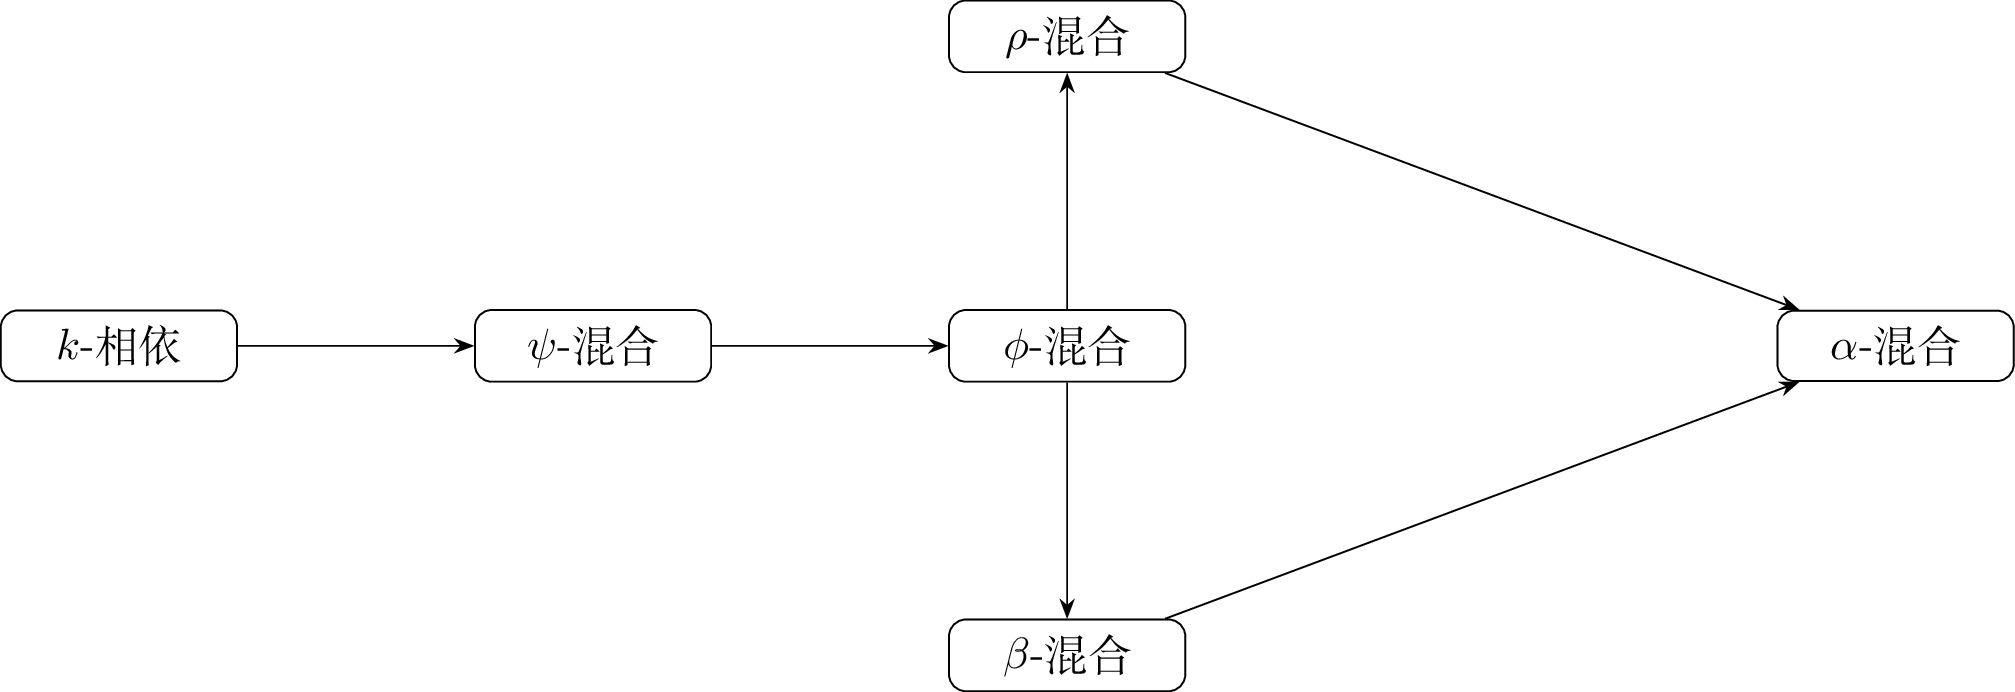
\includegraphics[width=0.94\textwidth]{figures/04-mixing-relations.png}
  \caption{各种混合条件之间的蕴含关系}
  \label{fig:ch4:mixing-relations}
\end{figure}

尽管 $\alpha$-混合的条件最弱，但它却被称作``强混合 (Strong Mixing)''，这纯属术语上的历史遗留问题。关于这些混合过程，可以参考一篇综述 \cite{bradley2005}。

一个自然的问题是：我们熟悉的模型满足这些混合性质吗？

\begin{itemize}
\tightlist
\item
  对于一个线性因果过程 $X_{t} = \sum_{j = 0}^{\infty} \psi_{j} \epsilon_{t - j}$：

\begin{itemize}
  \tightlist
  \item
    \cite{gorodetskii1978} 一文表明：在适当正则条件下， $X_t$ 是 $\alpha$ -混合的。
  \item
    如果系数 $\psi_j$ 以指数速率衰减（即 $\psi_{j} = O(\mu^{j})$，其中 $0 < \mu < 1$），那么该过程是\emph{几何 $\alpha$-混合}的，即存在常数 $C > 0$ 和 $\rho \in [0, 1)$，使得 $\alpha(k) \leq C \rho^k$。这个结论来自 \cite{tuanlanh1985}。
  \end{itemize}
\item
  对于 ARCH 过程：在一定的正则条件下，它们也具备遍历性并满足几何 $\alpha$-混合性质。例如，见 \cite{masrytjoestheim1995}。
\end{itemize}

\section{关于 α-混合系数的若干不等式}

本节证明若干 α-混合系数的基本的不等式，这些不等式表明：只要两个随机变量在时间上离得足够远，它们之间的相依性（协方差）就会被混合系数严格控制。

本节统一如下符号设定： $X,Y$ 是概率空间 $(\Omega,\mathcal F,P)$ 上的两个可积的实值随机变量， $\mathcal B,\mathcal C$ 是 $\mathcal F$ 的两个子 $\sigma$ -域，且 $X$ 为 $\mathcal B$ -可测， $Y$ 为 $\mathcal C$ -可测， $\alpha=\alpha(\mathcal B,\mathcal C)$ 。

\begin{lemma}[Billingsley 不等式]\label{lem:ch4:billingsley}

若 $|X| \leq C_1$，$|Y| \leq C_2$，那么
\[|\mathrm{Cov}(X, Y)| \leq 4C_1C_2\alpha\]
\end{lemma}

\begin{proof}

我们从协方差的定义出发，有：

\begin{equation}
\label{eq:ch4:tag-1}
|\mathrm{Cov}(X, Y)| = |\mathbb{E}[XY] -\mathbb{E}[X]\mathbb{E}[Y]| = \left|\mathbb{E}\Big[X\left(\mathbb{E}[Y|\mathcal{B}] - \mathbb{E}[Y]\right)\Big]\right|\leq C_1 \mathbb{E}\left[\Big|\mathbb{E}[Y|\mathcal{B}] - \mathbb{E}[Y]\Big|\right]
\end{equation}

令 $\xi := \operatorname{sgn}(\mathbb{E}[Y|\mathcal{B}] - \mathbb{E}[Y])$，显然 $\xi \in \mathcal{B}$ 且 $|\xi| \leq 1$。于是

\begin{equation}
\label{eq:ch4:tag-2}
\mathbb{E}\big[|\mathbb{E}[Y|\mathcal{B}] - \mathbb{E}[Y]| \big]= \mathbb{E}\left[\xi \left(\mathbb{E}[Y|\mathcal{B}] - \mathbb{E}[Y]\right)\right] = \mathbb{E}[\xi Y] - \mathbb{E}[\xi]\mathbb{E}[Y] = \mathrm{Cov}(\xi, Y)
\end{equation}

因此，

\begin{equation}
\label{eq:ch4:tag-3}
|\mathrm{Cov}(X, Y)| \leq C_1 |\mathrm{Cov}(\xi, Y)|
\end{equation}

使用同样的方法，我们对 $Y$ 和 $\xi$ 应用上述过程。令 $\eta = \operatorname{sgn}(\mathbb{E}[\xi|\mathcal{C}] - \mathbb{E}[\xi])$，则 $\eta \in \mathcal{C}$ 且 $|\eta| \leq 1$，类似地可得
\[|\mathrm{Cov}(\xi, Y)| \leq C_2 |\mathrm{Cov}(\xi, \eta)|\]
现在分析 $|\mathrm{Cov}(\xi, \eta)| = |\mathbb{E}[\xi\eta] - \mathbb{E}[\xi]\mathbb{E}[\eta]|$。由于 $\xi$ 和 $\eta$ 都是取值为 $\pm 1$ 的随机变量，我们可以通过事件概率来表示。令
\[\begin{gathered}A = \{\xi = 1\}, \quad B = \{\eta = 1\}\\ A^c = \{\xi = -1\}, \quad B^c = \{\eta = -1\} \end{gathered}\]
显然 $A, A^c \in \mathcal{B}$ 且 $B, B^c \in \mathcal{C}$。于是，
\[\begin{aligned} |\mathbb{E}[\xi\eta] - \mathbb{E}[\xi]\mathbb{E}[\eta]| &= |P(A \cap B) + P(A^c \cap B^c) - P(A^c \cap B) - P(A \cap B^c)| \\ &\leq |P(A \cap B) - P(A)P(B)| + |P(A^c \cap B^c) - P(A^c)P(B^c)| \\ &\quad + |P(A^c \cap B) - P(A^c)P(B)| + |P(A \cap B^c) - P(A)P(B^c)| \\ &\leq 4\alpha(k)  \end{aligned}\]
结合式~\eqref{eq:ch4:tag-1}、\eqref{eq:ch4:tag-2} 和 \eqref{eq:ch4:tag-3}，引理即证。

\end{proof}

\begin{lemma}[有界变量的协方差界]\label{lem:ch4:covariance-lp-bound}

若 $\mathbb{E}[|X|^{p}] < \infty$ 对某个 $p > 1$ 成立，且 $|Y| \leq C$，则
\[|\mathrm{Cov}(X, Y)| \leq 6C \|X\|_{p} \alpha^{1/q}\]
其中 $\frac{1}{p} + \frac{1}{q} = 1$，且 $\|X\|_p := (\mathbb{E}[|X|^p])^{1/p}$。

\end{lemma}

\begin{proof}

我们采用截断技术。对某个 $M > 0$，令
\[X_{M} = X\mathbb{I}(|X|\leq M), \quad X'_{M} = X - X_{M} = X\mathbb{I}(|X| > M)\]
则 $X = X_{M} + X'_{M}$。根据协方差的线性性质，
\[|\mathrm{Cov}(X,Y)| = |\mathrm{Cov}(X_{M},Y) + \mathrm{Cov}(X_{M}^{\prime},Y)|\leq |\mathrm{Cov}(X_{M},Y)| + |\mathrm{Cov}(X'_{M},Y)|\]
首先处理第一项。由于 $|X_M| \leq M$ 且 $|Y| \leq C$，由引理~\ref{lem:ch4:billingsley} 有

\begin{equation}
\label{eq:ch4:tag-4}
|\mathrm{Cov}(X_{M},Y)|\leq 4CM\alpha
\end{equation}

其次处理第二项，我们有
\[\begin{aligned} \mathbb{E}[|X_{M}'|] &= \int_{|X| > M}|x|\mathrm{d}F(x) \\ &\leq \int_{|X| > M}|x|\left(\frac{|x|}{M}\right)^{p-1}\mathrm{d}F(x) \\ &\leq M^{-(p-1)}\int_{-\infty}^{\infty} |x|^p \mathrm{d}F(x) = M^{1-p}\mathbb{E}[|X|^{p}] \end{aligned}\]
因此，

\begin{equation}
\label{eq:ch4:tag-5}
|\mathrm{Cov}(X_M',Y)| = |\mathbb{E}[X_M'Y] - \mathbb{E}[X_M']\mathbb{E}[Y]| \leq \mathbb{E}[|X_M'Y|] + C\mathbb{E}[|X_M'|] \leq 2C\mathbb{E}[|X_M'|] \leq 2C M^{1-p}\mathbb{E}[|X|^p]
\end{equation}

现在，为了最小化式~\eqref{eq:ch4:tag-4} 和 \eqref{eq:ch4:tag-5} 的和，我们选择 $M$ 使得两项平衡。取
\[M = \| X\| _p\alpha ^{- 1 / p}\]
将 $M$ 分别代入式~\eqref{eq:ch4:tag-4} 和 \eqref{eq:ch4:tag-5}：
\[|\mathrm{Cov}(X_{M},Y)|\leq 4C \| X\| _p\alpha ^{- 1 / p} \alpha  = 4C \| X\| _p \alpha^{1 - 1/p} = 4C \| X\| _p\alpha^{1/q}\]\[|\mathrm{Cov}(X_M',Y)| \leq 2C \left(\| X\| _p \alpha^{-1/p}\right)^{1-p} \mathbb{E}[|X|^p] = 2C \| X\| _p^{1-p} \alpha^{(p-1)/p} \| X\| _p^p = 2C \| X\| _p \alpha^{1/q}\]
将两式相加即证。

\end{proof}

引理~\ref{lem:ch4:covariance-lp-bound} 是引理~\ref{lem:ch4:billingsley} 的推广：后者只是前者在 $p=\infty,q=1$ 的特例。

\begin{lemma}[Rio 不等式]\label{lem:ch4:rio}

令 $Q_{X}(u) = \inf \{t: P(|X| > t) \leq u\}$ 为 $|X|$ 的分位数函数。如果 $Q_{X}Q_{Y}$ 在 $(0,1)$ 上可积，则
\[|\mathrm {Cov}(X,Y)|\leq 2\int_{0}^{2\alpha}Q_{X}(u)Q_{Y}(u)\mathrm{d}u\]
\end{lemma}

\begin{proof}

我们将随机变量 $X$ 和 $Y$ 分解为其正部和负部：$X = X^{+} - X^{-}$，$Y = Y^{+} - Y^{-}$，其中 $X^{+} = \max(0, X)$，$X^{-} = \max(0, -X)$。利用协方差的线性性质，可得

\begin{equation}
\label{eq:ch4:tag-6}
\mathrm{Cov}(X,Y) = \mathrm{Cov}(X^{+},Y^{+}) + \mathrm{Cov}(X^{-},Y^{-}) - \mathrm{Cov}(X^{-},Y^{+}) - \mathrm{Cov}(X^{+},Y^{-})
\end{equation}

对于任意两个非负随机变量 $U$ 和 $V$，不难验证其协方差可以写作：

\begin{equation}
\label{eq:ch4:tag-7}
\mathrm{Cov}(U,V) = \int_{0}^{\infty} \!\!\int_{0}^{\infty} \Big( P(U > u, V > v) - P(U > u)P(V > v) \Big)\mathrm{d}u \mathrm{d}v
\end{equation}

将此式应用于 $X^{+}$ 和 $Y^{+}$，我们得到：
\[\mathrm{Cov}(X^{+},Y^{+}) = \int_{0}^{\infty} \!\!\int_{0}^{\infty} \Big( P(X^{+} > u, Y^{+} > v) - P(X^{+} > u)P(Y^{+} > v) \Big)  \mathrm{d}u  \mathrm{d}v\]
根据 $\alpha$-混合系数的定义，对任意事件 $A \in \sigma(X)$ 和 $B \in \sigma(Y)$，有 $|P(A \cap B) - P(A)P(B)| \leq \alpha$。同时，联合概率 $P(A \cap B)$ 显然不会超过边缘概率 $P(A)$ 或 $P(B)$。因此，被积函数中的概率差值的绝对值可以被 $\min \big\{\alpha, P(X^{+} > u), P(Y^{+} > v) \big\}$ 所控制。从而有：
\[\mathrm{Cov}(X^{+},Y^{+}) \leq \int_{0}^{\infty} \!\!\int_{0}^{\infty}\min \big\{ \alpha, P(X^{+} > u), P(Y^{+} > v) \big\} \mathrm{d}u  \mathrm{d}v\]
我们将式~\eqref{eq:ch4:tag-6} 中的四项协方差全部用形如式~\eqref{eq:ch4:tag-7} 的形式进行放缩，并利用如下的初等结论：对任意非负实数 $a, b, c, d$ 和 $\alpha > 0$，有
\[(\alpha \wedge a \wedge c) + (\alpha \wedge a \wedge d) + (\alpha \wedge b \wedge c) + (\alpha \wedge b \wedge d) \leq 2\big[ (2\alpha) \wedge (a + b) \wedge (c + d) \big]\]
将此不等式应用于 $a = P(X > u), b = P(-X > u), c = P(Y > v), d = P(-Y > v)$ ，我们可以将四项积分合并，得到：
\[|\mathrm{Cov}(X,Y)| \leq 2\int_{0}^{\infty} \!\!\int_{0}^{\infty}\min \big\{ 2\alpha, P(|X| > u), P(|Y| > v) \big\} \mathrm{d}u  \mathrm{d}v =: \mathcal{I}\]
最后一步是证明积分 $\mathcal{I}$ 等于定理中给出的形式。考虑均匀分布随机变量 $U\sim\mathcal U([0,1])$，并基于它定义：
\[Z:=\begin{cases} Q_X(U),&\text{ 若 }U<2\alpha\\ 0,&\text{ 若 }U\ge 2\alpha \end{cases}\quad T:=\begin{cases} Q_Y(U),&\text{ 若 }U<2\alpha\\ 0,&\text{ 若 }U\ge 2\alpha \end{cases}\]
则有：
\[\mathbb{E}[ZT] = \int_{0}^{2\alpha} Q_{X}(u) Q_{Y}(u) \, \mathrm{d}u\]
另一方面，事件 $\{Z > u, T > v\}$ 发生当且仅当 $U < 2\alpha$ 且同时满足 $U < P(|X| > u)$ 和 $U < P(|Y| > v)$。因此，
\[P(Z > u, T > v) = \mathbb{P}\big(U < 2\alpha, U < P(|X| > u), U < P(|Y| > v) \big) = \min\big\{ 2\alpha, P(|X| > u), P(|Y| > v) \}\]
由于 $Z$ 和 $T$ 非负，我们再次使用前述积分恒等式，得到：
\[\mathbb{E}[ZT] =\int_{0}^{\infty} \!\!\int_{0}^{\infty}P(Z > u, T > v) \mathrm{d}u \mathrm{d}v = \int_{0}^{\infty} \!\!\int_{0}^{\infty}\min\big\{ 2\alpha, P(|X| > u), P(|Y| > v) \big\}  \mathrm{d}u \mathrm{d}v = \frac{1}{2} \mathcal{I}\]
比较 $\mathbb{E}[ZT]$ 的两个表达式，便有 $\mathcal{I} = 2 \int_{0}^{2\alpha} Q_{X}(u) Q_{Y}(u) \, \mathrm{d}u$。

\end{proof}

利用引理~\ref{lem:ch4:rio}，我们可推导出经典的 Davydov 不等式，这是处理混合相依序列矩不等式的一项核心工具，

\begin{lemma}[Davydov 不等式]\label{lem:ch4:davydov}

令 $X$ 和 $Y$ 满足 $X \in L^q(\mathcal{B})$，$Y \in L^r(\mathcal{C})$，其中 $q > 1$，$r > 1$ 且 $\frac{1}{q} + \frac{1}{r} = 1 - \frac{1}{p}$，则
\[|\mathrm{Cov}(X, Y)| \leq 2p(2\alpha(k))^{1/p} \|X\|_q \|Y\|_r\]
\end{lemma}

\begin{proof}

分三种情况。

\begin{enumerate}
\def\labelenumi{\arabic{enumi}.}
\tightlist
\item
  $q$ 和 $r$ 均为有限的情形
\end{enumerate}

由 Markov 不等式，
\[P\left(|X| > \frac{\|X\|_q}{u^{1 / q}}\right) \leq \frac{\mathbb{E}|X|^q}{\left(\|X\|_q / u^{1 / q}\right)^q} = u, \quad 0 < u \leq 1\]
根据分位数函数 $Q_X$ 的定义，上式说明
\[Q_X(u) \leq \frac{\|X\|_q}{u^{1 / q}}, \quad 0 < u \leq 1\]
类似地，$Q_Y(u) \leq \|Y\|_r / u^{1 / r}$。使用 Rio 不等式（引理~\ref{lem:ch4:rio}），
\[\begin{aligned} |\mathrm {Cov}(X, Y)| & \leq 2 \int_0^{2\alpha} \frac{\|X\|_q \|Y\|_r}{u^{1 / q} u^{1 / r}} \mathrm{d}u \\ & = 2 \|X\|_q \|Y\|_r \int_0^{2\alpha} u^{\frac{1}{p} - 1} \mathrm{d}u \\ & = 2 p(2\alpha )^{1 / p} \|X\|_q \|Y\|_r \end{aligned}\]
\begin{enumerate}
\def\labelenumi{\arabic{enumi}.}
\setcounter{enumi}{1}
\tightlist
\item
  $r = \infty$，$q$ 有限的情形
\end{enumerate}

此时 $\frac{1}{q} + \frac{1}{p} = 1$。注意到， $Q_Y(u) \leq Q_Y(0) = \|Y\|_\infty = \sup |Y|$ ，再次用 Rio 不等式，
\[| \mathrm{Cov}(X, Y) | \leq 2 \int_0^{2\alpha} \frac{\|X\|_q}{u^{1/q}} \|Y\|_\infty \mathrm{d}u = 2 \|X\|_q \|Y\|_\infty \int_0^{2\alpha} u^{\frac{1}{p}-1} \mathrm{d}u = 2p(2\alpha)^{1/p} \|X\|_q \|Y\|_\infty\]
这与引理~\ref{lem:ch4:covariance-lp-bound} 相似但不全相同。

\begin{enumerate}
\def\labelenumi{\arabic{enumi}.}
\setcounter{enumi}{2}
\tightlist
\item
  $r = +\infty$ 且 $q = +\infty$ 的情形
\end{enumerate}

此时 $p = 1$。再次使用 Rio 不等式，
\[|\mathrm {Cov}(X,Y)|\leq 2\int_{0}^{2\alpha }\| X\|_{\infty}\| Y\|_{\infty}\mathrm{d}u = 4\| X\|_{\infty}\| Y\|_{\infty}\alpha\]
这与引理~\ref{lem:ch4:billingsley} 完全相同。

\end{proof}

关于这些不等式，推荐读者参考 \cite{bosq1996} 一书的第一章。也可参阅 \cite{lulingzhengyan1997} 一书的 §1.2。

最后给出 Davydov 不等式（引理~\ref{lem:ch4:davydov}）的一个具体应用。

\begin{definition*}[长记忆与短记忆过程]
设 $\{X_t\}_{t\in\mathbb Z}$ 是一个二阶矩有限的宽平稳过程。令 $\gamma(k)=\mathrm{Cov}(X_i,X_{i+k})$ 是其自协方差函数 (ACVF)。

\begin{itemize}
\tightlist
\item
  如果 $\sum_{k=0}^{\infty} |\gamma(k)| = \infty$，则它是一个\textbf{\emph{长记忆过程}} (Long Memory Process)。
\item
  如果 $\sum_{k=0}^{\infty} |\gamma(k)| < \infty$，我们称该过程为\textbf{\emph{短记忆过程}} (Short Memory Process) 。
\end{itemize}
\end{definition*}

长记忆与短记忆这两个术语最早见 \cite{mcleodhipel1978}。

利用 Davydov 不等式（取 $r = q$），如果 $\mathbb{E}[|X_i|^q ]< \infty$ 对 $q > 2$ 成立，且 $\sum_{k = 0}^{\infty} (\alpha(k))^{1 / p} < \infty$ 对 $p = \frac{q}{q - 2}$ 成立，则
\[\sum_{k=0}^\infty|\gamma(k)|\le 2p\|X\|_q^2\sum_{k=0}^\infty(\alpha(k))^{1/p}<\infty\]
说明该过程是短记忆的。

特别地，如果 $\alpha (k) \leq C \rho^k$ ，即``几何强混合 (GSM)''，则
\[\sum_{k = 0}^{\infty} (\alpha(k))^{1 / p} \leq C \sum_{k = 0}^{\infty} \rho^{k / p} = \frac{C}{1 - \rho^{1 / p}} < \infty .\]
通常，为了保证 $\sum_{k=0}^\infty (\alpha(k))^{1/p} < \infty$，只需要 $(\alpha(k))^{1/p} \sim k^{-(1+\eta)}$，即当 $k$ 充分大时 $\alpha(k) \sim k^{-p(1+\eta)}$ 对某个 $\eta > 0$ 成立；几何强混合意味着 $\alpha(k) \leq C\rho^k$，其衰减速度是指数级的，条件更强。

\section{α-混合序列的中心极限定理}

关于混合相依变量的弱收敛，有非常多的理论，除了本节要介绍的 α-混合序列中心极限定理外，还有一些研究放宽了矩条件或平稳性条件，或是研究其它混合系数下的弱收敛，或是弱不变原理等；除了这些渐近结论，还有类比于 Hoeffding 不等式、Bernstein 不等式这样的非渐近不等式（但对于相依序列而言结论十分复杂，并且其界与混合系数有关）。限于篇幅，无法一一叙述。

\subsection{准备工作}

首先的一个结论可以类比于弱大数律：

\begin{theorem}[长程方差的存在性]
\label{thm:ch4:long-run-variance}

令 $\{X_t\}_{t \in \mathbb{Z}}$ 是一个零均值、实值的弱平稳过程，满足对某个 $r > 2$，
\[\sup_{t\in \mathbb{Z}}\mathbb{E}[|X_t|^r ]< \infty ,\quad \sum_{k\geq 1}\alpha (k)^{1 - \frac{2}{r}}< \infty\]
则级数 $\sum_{k\in \mathbb{Z}}\gamma (k)$ 绝对收敛，且收敛到一个非负和 $\sigma^2$，使得
\[\lim_{n\to \infty}n\mathrm{Var}(S_n / n) = \sigma^2\]
其中 $\gamma (k) := \mathrm{Cov}(X_i, X_{i+k})$ 是自协方差函数， $S_n:=\sum_{t=1}^nX_t$ 代表连续 $n$ 项和。

\end{theorem}

\begin{remark}

\begin{itemize}
\tightlist
\item
  注意，由于宽平稳性， $\gamma(k)=\mathrm{Cov}(X_i,X_{i+k})$ 的值和 $i$ 无关；同样， $S_n$ 的起点选择也和其分布无关。
\item
  这里的 $\sigma^2$ 又叫做\textbf{\emph{长程方差}} (Long-run Variance)。
\end{itemize}
\end{remark}

\begin{proof}

首先我们研究级数 $\sum_{k \in \mathbb{Z}} \gamma(k)$ 的收敛性。使用 Davydov 不等式（引理~\ref{lem:ch4:davydov}），取 $q = r$ 且 $\frac{1}{p} = 1 - \frac{2}{r}$，得到
\[|\gamma (k)| \leq 2p (2\alpha(k))^{1/p} \|X_0\|_r \|X_k\|_r \leq 2p (2\alpha(k))^{1 - 2/r} \sup_{t\in\mathbb{Z}}\|X_t\|_r^2\]
由于 $\sum_{k \geq 1} \alpha (k)^{1 - 2 / r} < +\infty$，根据比较判别法，级数 $\sum_k |\gamma(k)|$ 绝对收敛。

现在考虑 $n \mathrm{Var} (S_n / n)$，
\[n \mathrm{Var}\! \left(\frac{S_n}{n}\right) = n^{-1} \sum_{0 \leq s, t \leq n - 1} \mathrm{Cov}(X_s, X_t) = \sum_{k = -(n - 1)}^{n - 1} \left(1 - \frac{|k|}{n}\right) \gamma (k)\]
根据控制收敛定理，当 $n \to \infty$ 时，
\[\lim_{n \to \infty} n \mathrm{Var}\! \left(\frac{S_n}{n}\right) = \sum_{k=-\infty}^\infty \gamma(k) = \sigma^2 \geq 0\]
定理得证。

\end{proof}

第二个工具叫做\textbf{\emph{耦合方法}} (Coupling Method) ，这是一种将``变量间存在依赖性的平稳随机序列''转变为``彼此独立的随机变量序列''的手段。简而言之，给定一个具有复杂相依关系的随机向量 $(X,Y)\in\mathbb R^k\times\mathbb R$，我们构造一个新的随机变量 $Y^*$，使得它与 $Y$ 同分布，但与 $X$ 独立，并且 $Y^*$ 和 $Y$ 尽可能接近。相关的结论如下：

\begin{lemma}[Bradley 引理]\label{lem:ch4:bradley}

令随机向量 $(X,Y)\in \mathbb{R}^d\times \mathbb{R}$ ，满足 $Y\in L^p(P)$ ， $p\in [1,\infty)$。令 $c$ 为一个实数，使得 $\| Y + c\| _p > 0$，并令 $\xi \in (0,\| Y + c\| _p]$。则存在一个随机变量 $Y^{*}$ 满足：

\begin{enumerate}
\def\labelenumi{\arabic{enumi}.}
\tightlist
\item
  $P_{Y^{*}} = P_{Y}$ ；
\item
  $Y^{*}$ 与 $X$ 独立；
\item
  \[
  P(|Y-Y^*|>\xi)
  \leq 11(\xi^{-1}\|Y+c\|_p)^{p/(2p+1)}
  \bigl(\alpha(\sigma(X),\sigma(Y))\bigr)^{2p/(2p+1)}.
  \]
\end{enumerate}

\end{lemma}
来自 \cite{bradley1983} 一文的 Theorem 3。在该论文中，这里的常数 11 原本是 18 且 $c = 0$，但证明过程是一致的。

最后还有一个引理，帮助我们后文中阶的估算


\begin{lemma}[横山良三矩界]\label{lem:ch4:yokoyama}

设 $\{X_t\}_{t\in \mathbb Z}$ 是零均值、实值、严平稳的 α-混合过程，满足：存在 $\gamma>2$ 和 $\delta>0$ 使得 $\mathbb{E}[|X_t|^{\gamma+\delta}] < \infty$ 。若
\[
\sum_{k=1}^\infty(k+1)^{\gamma/2-1}(\alpha(k))^{\frac\delta{\gamma+\delta}}<\infty,
\]

那么存在常数 $C$ 使得对每个 $n\ge 1$ ， $\mathbb{E}[|S_n|^\gamma]\le Cn^{\gamma/2}$

\end{lemma}
该引理来自 \cite{yokoyama1980} 一文的 Theorem 1。


\begin{corollary}\label{cor:ch4:moment-bound}
设 $\{X_t\}_{t\in \mathbb Z}$ 是零均值实值严平稳过程，满足：存在 $\gamma > 2$ 和 $\beta > 1$，使得
\[\mathbb{E}[|X_t|^\gamma] < \infty , \quad \alpha (k) \leq a k^{-\beta}\]
其中 $a$ 为正常数，且 $\beta > \gamma / (\gamma - 2)$。那么存在常数 $C$ 和 $\gamma'\in(2,\gamma)$ 使得对每个 $n\ge 1$，$\mathbb{E}[|S_n|^{\gamma'}]\le Cn^{\gamma'/2}$。
\end{corollary}

\begin{proof}

根据引理~\ref{lem:ch4:yokoyama}，我们只需证明 
$$\sum_{k=1}^\infty(k+1)^{\gamma'/2-1}(\alpha(k))^{\frac{\gamma-\gamma'}{\gamma}}<\infty$$
代入 $\alpha (k) \leq a k^{-\beta}$ ，上式等价于 $\frac{\gamma'}2-1-\beta\frac{\gamma-\gamma'}{\gamma}<-1$ ，即 $\gamma'<\frac{2\beta\gamma}{2\beta+\gamma}$ 。另一方面， $\beta > \gamma / (\gamma - 2)$ 保证了 $\frac{2\beta\gamma}{2\beta+\gamma}=((2\beta)^{-1}+\gamma^{-1})^{-1}>((2\gamma/(\gamma-2))^{-1}+\gamma^{-1})^{-1}=2$ ，即区间 $\left(2,\frac{2\beta\gamma}{2\beta+\gamma}\right)$ 非空，总是可以做到从中取 $\gamma'$ 的。

\end{proof}

\subsection{α-混合序列的中心极限定理和证明}

对严平稳 α-混合随机序列，I. A. Ibragimov 最早给出了其中心极限定理的充要条件，但相当繁琐，不易验证。下面的定理是一个充分条件， 来自 \cite{bosq1996} 书中的 Theorem 1.7。

\begin{theorem}[$\alpha$-混合序列的中心极限定理]
\label{thm:ch4:alpha-mixing-clt}

令 $\{X_{t}\}_{t\in \mathbb{Z}}$ 是零均值实值严平稳过程，满足：存在 $\gamma > 2$ 和 $\beta > 1$， 使得
\[\mathbb{E}[|X_t|^\gamma] < \infty , \quad \alpha (k) \leq a k^{-\beta}\]
其中 $a$ 为正常数，且 $\beta > \gamma / (\gamma - 2)$。如果 $\sigma^2 = \sum_{k = -\infty}^{\infty} \gamma (k) > 0$，则有
\[\frac{S_n}{\sigma\sqrt{n}} \overset{\rm d}\to\mathcal N(0,1)\]
\end{theorem}

\begin{proof}

为清晰起见，我们分成六步。

\emph{第一步}：首先，由定理~\ref{thm:ch4:long-run-variance}，我们知道自协方差 $\gamma(k)$ 满足绝对收敛 $\sum_{k=-\infty}^\infty |\gamma(k)| < \infty$，从而 $\sigma^2$ 是良定义的。

\emph{第二步}：应用 \textbf{\emph{Bernstein Blocking Method }}：将序列 $X_1,\dots,X_n$ 分割为长度为 $p$ 的大块和长度为 $q$ 的小块，按``大块-小块-大块-小块-\ldots{}''交替排列，并让其长度满足：

\begin{itemize}
\tightlist
\item
  $p\sim\frac n{\log n}-n^{1/4}$ ；
\item
  $q\sim n^{1/4}$ 。
\end{itemize}

则共有 $r:=\left[\frac n{p+q}\right]\sim \log n$ 个大块和小块，并且由于被小块分隔开的缘故，大块之间是近似独立的。

记大块内随机变量的和为 $Y_i$ ，小块内的和为 $Z_i$ ， $i=1,\dots,r$ ，从而 $S_n$ 可写作
\[
\begin{aligned}
S_n={}&\underbrace{(X_1+ \cdots+ X_p)}_{Y_1} + \underbrace{(X_{p+1}+ \dots +X_{p+q})}_{Z_1}\\
&+ \underbrace{(X_{p+q+1} +\dots +X_{2p+q})}_{Y_2}+ \underbrace{(X_{2p+q+1}+ \dots +X_{2p+2q})}_{Z_2}+\dots\\
&+ \underbrace{(X_{(r-1)(p+q)+1} +\dots +X_{rp+(r-1)q})}_{Y_r}\\
&+\underbrace{(X_{rp+(r-1)q+1}+ \dots +X_{r(p+q)})}_{Z_r} + \text{余项 } R_r.
\end{aligned}
\]
第三步：考虑对每个大块应用 Bradley 引理（引理~\ref{lem:ch4:bradley}），从而得到一系列独立的副本 $Y^*_i$ ，且 $Y_i$ 与 $Y^*_i$ 足够接近。我们按照如下方式构造副本 $Y_i^*$：

\begin{itemize}
\tightlist
\item
  对于 $i = 1$ ，取 $Y_1^*=Y_1$ ；
\item
  对于 $i \ge 2$，将 Bradley 引理应用于：$(Y_1,Y_2,\dots,Y_{i-1})$ 和 $Y_i$，得到 $Y_i^*$ 。取常数 $c = \zeta p \|X_0\|_\gamma$（ $\zeta > 1$ ）、 $\xi = \frac{\epsilon \sigma \sqrt{n}}{r}$（ $\epsilon > 0$ 充分小）。此时对足够大的 $n$，
  \[
  \|Y_i+c\|_\gamma
  \ge c-\|Y_i\|_\gamma
  \ge (\zeta-1)p\|X_0\|_\gamma
  \ge \frac{\epsilon\sigma\sqrt n}{r}
  =\xi,
  \]
  从而 Bradley 引理的条件成立；上面最后一个不等式用到了 $p\sim\frac n{\log n}$ 的阶大于 $\frac{\sqrt n}r\sim\frac{\sqrt n}{\log n}$ 的阶。
\end{itemize}

由此得到了 i.i.d. 的 $Y_1^*,\dots,Y_r^*$ ，且\[ P\left( |Y_i - Y^*_i| > \frac{\epsilon \sigma \sqrt{n}}{r} \right) \leq 11 \left( \frac{\|Y_i + c\|_\gamma}{\xi} \right)^{\frac{\gamma}{2\gamma+1}} \alpha(q)^{\frac{2\gamma}{2\gamma+1}} \] 对 $i$ 求和，记\[ \Delta_n := \frac{\sum_{i=1}^r Y_i}{\sigma \sqrt{n}} - \frac{\sum_{i=1}^r Y^*_i}{\sigma \sqrt{n}} = \frac{1}{\sigma\sqrt{n}} \sum_{i=1}^r (Y_i - Y^*_i) \]

则
\[P(|\Delta_n| > \epsilon) \leq \sum_{i=1}^r P\left( |Y_i - Y^*_i| > \frac{\epsilon \sigma \sqrt{n}}{r} \right) \leq 11 r \left( \frac{\|Y_1 + c\|_\gamma}{\xi} \right)^{\frac{\gamma}{2\gamma+1}} \alpha(q)^{\frac{2\gamma}{2\gamma+1}}.\]记上式右侧为 $m_n$，由 $\|Y_i+c\|_\gamma/\xi=O(pr/\sqrt n)=O(\sqrt n)$，可知 $m_n$ 的阶数为
\[\begin{aligned}m_n &= O\left( r \cdot n^{\frac{\gamma}{4\gamma+2}} \cdot \alpha([n^{1/4}])^{\frac{2\gamma}{2\gamma+1}} \right)\\ &= O\left( \log n\cdot n^{\frac{\gamma}{4\gamma+2}} \cdot n^{-\frac{\beta \gamma}{2(2\gamma+1)}} \right)\\ &=O\left(\log n\cdot n^{-\frac{(\beta-1)\gamma}{4\gamma+2}}\right)\\ &\to 0 \end{aligned}\]
即 $\Delta_n\overset{P}\to 0$ 。

第五步：我们表明上一步中构造的 i.i.d. 副本 $Y_1^*,\dots,Y_n^*$ 满足中心极限定理。首先，显然 \[ \mathbb{E}\big[{Y^*_i}^2\big]=\mathbb{E}[Y_i^2]=\mathbb{E}[S_p^2]\sim \sigma^2p \]由推论~\ref{cor:ch4:moment-bound}，存在 $2<\gamma'<\gamma$ 使得 $\mathbb{E}[|Y_i|^{\gamma'}]\le Cp^{\gamma'/2}$，$i=1,\dots,r$。从而
\[
\begin{aligned}
\sum_{i=1}^r
\frac{\mathbb E[|Y^*_j|^{\gamma'}]}
{\left(\mathrm{Var}\left[\sum_{i=1}^rY^*_j\right]\right)^{\gamma'/2}}
&=O\left(r\frac{Cp^{\gamma'/2}}{(r\sigma^2p)^{\gamma'/2}}\right)\\
&=O\left(r^{1-\gamma'/2}\right)\to 0.
\end{aligned}
\]
Lyapunov 条件得以满足，独立和 $\sum_{j=1}^r Y_j^*$ 的中心极限定理成立：
\[\frac{Y_1^*+\cdots+Y_n^*}{\sigma\sqrt n}=\underbrace{\left(\frac{rp}{n}\right)^{1/2}}_{\to 1}\frac{Y_1^*+\cdots+Y_n^*}{\sigma\sqrt{rp}}\overset{\rm d}\to \mathcal N(0,1)\]
从而，根据 Slutsky 定理， \[ \frac{Y_1+\cdots+Y_n}{\sigma\sqrt n}=\frac{Y_1^*+\cdots+Y_n^*}{\sigma\sqrt n}+\underbrace{\Delta_n}_{o_P(1)}\overset{\rm d}\to\mathcal N(0,1) \]第六步：与四、五步完全相同地，对小块也有中心极限定理成立： \[ \frac{Z_1+\cdots+Z_n}{\sigma\sqrt{rq}}\overset{\rm d}\to \mathcal N(0,1) \]那么 \[ \frac{Z_1+\cdots+Z_n}{\sigma\sqrt{n}}=\underbrace{\left(\frac{rq}{n}\right)^{1/2}}_{\to 0}\frac{Z_1+\cdots+Z_n}{\sigma\sqrt{rq}}\to 0 \]所以根据 Slutsky 定理，小块的部分是可忽略的。

至于尾部余项 $R_r$，由于其长度不超过 $p+q$，由 Chebyshev 不等式，
\[P\left( \frac{|R_r|}{\sigma \sqrt{n}} > \epsilon \right) \leq \frac{\mathrm{Var}(R_r)}{\epsilon^2 \sigma^2 n} = O\left( \frac{\sigma^2(p+q)}{\epsilon^2\sigma^2n} \right) = O\left( \frac{1}{\log n} \right) \to 0\]
自然也是可忽略的。至此，我们完成了证明。

\end{proof}

最后，我们整理一下上述证明思路：

\begin{itemize}
\tightlist
\item
  定理~\ref{thm:ch4:long-run-variance} 保证 $\sigma^2$ 存在且有限。
\item
  用 Bernstein Blocking Method 将 $X_1,X_2,\dots,X_n$ 划分为大块、以及把大块分隔开的小块。
\item
  用 Bradley 引理为每个大块内元素和 $Y_i$ 提供独立同分布的副本 $Y_i^*$ 。
\item
  证明副本 $Y_i^*$ 满足 Lyapunov 中心极限定理。
\item
  副本 $Y_i^*$ 和原来的 $Y_i$ 之间的差距是可忽略的，小块和余项也是可忽略的，所以总体便成立中心极限定理。
\end{itemize}

\section{如何估计长程方差？------谱方法入门}

根据定理~\ref{thm:ch4:alpha-mixing-clt}， $S_n/\sqrt n$ 的渐近方差就是所谓的长程方差 $\sigma^2 = \sum_{k=-\infty}^\infty \gamma(k)=\gamma(0)+2\sum_{k=1}^\infty\gamma(k)$。如果我们能有对 $\sigma^2$ 的很好的估计，就能解决构建置信区间、或是进行假设检验等统计问题。但如何从数据中估计这个包含了所有自协方差的量呢？通常的方法是借助频域谱分析。

\subsection{谱密度函数}

\begin{definition*}[谱分布函数与谱密度函数]
对于实值宽平稳过程 $\{X(t)\}_{t\in T}$ 和其自协方差函数 $\gamma(k)$，如果有 $[-\pi,\pi]$ 上单调不减右连续的函数 $F(\lambda)$ 使得 $F(-\pi)=0$，且对每个 $k\in\mathbb Z$ 成立 $\gamma(k)=\int_{-\pi}^\pi e^{ik\lambda}\mathrm{d}F(\lambda)$，则称 $F(\lambda)$ 是 $X(t)$ 或 $\gamma(k)$ 的\textbf{\emph{谱分布函数}} (spectral distribution function)。如果有 $[-\pi,\pi]$ 上的非负函数 $f(\lambda)$ 使得对每个 $k\in\mathbb Z$ 成立 $\gamma(k)=\int_{-\pi}^\pi f(\lambda)e^{ik\lambda}\mathrm{d}\lambda$，则称 $f(\lambda)$ 是 $X(t)$ 或 $\gamma(k)$ 的\textbf{\emph{谱密度函数}} (spectral density function)，又称功率谱。
\end{definition*}

Herglotz 定理保证了 $F(\lambda)$ 的唯一存在性。若 $F(\lambda)$ 和 $f(\lambda)$ 同时存在，则 $F(\lambda)=\int_{-\pi}^\lambda f(s)\mathrm{d}s$ 。

关于谱密度函数，更常见的另一种定义如下，当 $\gamma(k)$ 绝对可和（即级数绝对收敛）： $\sum_{-\infty}^\infty |\gamma(k)|<\infty$ ，则 \[ f(\lambda)=\frac1{2\pi}\sum_{k=-\infty}^\infty e^{ik\lambda}\gamma(k) \]就是谱密度函数。可见 \cite{brockwelldavis2006} 一书的 Theorem 4.3.2 和 Corollary 4.3.2 等。进一步，由 Weierstrass M-判别法，上述级数一致收敛，从而 $f(\lambda)$ 在 $[-\pi,\pi]$ 上一致连续。

\begin{example}[ARMA 过程的谱密度]
设有 $\mathrm{ARMA}(p,q)$ 过程 $\theta(B)X_t = \eta(B)\epsilon_t$，$\epsilon_t\sim \mathrm{WN}(0, \sigma^2)$，满足定理~\ref{thm:ch4:arma-causality} 的因果性条件，使得 $X_t=\psi(B)\epsilon_t=\sum_{j=0}^\infty\psi_j\epsilon_{t-j}$，其中 $\psi(z)=\frac{\eta(z)}{\theta(z)}=\sum\limits_{j=0}^\infty\psi_jz^j,\enspace |z|\le 1$。其自协方差函数为（不失一般性设 $k\ge 0$）：
\[\begin{aligned} \gamma(k)&=\mathbb{E}[X_tX_{t+k}]\\ &=\mathbb{E}\!\left[\left(\sum_{j=0}^\infty\psi_j\epsilon_{t-j}\right)\left(\sum_{l=0}^\infty\psi_l\epsilon_{t+k-l}\right)\right]\\ &=\sum_{j=0}^\infty\sum_{l=0}^\infty \psi_j\psi_l\mathbb{E}[\epsilon_{t+j}\epsilon_{t+k-l}]\\ &=\sigma^2\sum_{j=0}^\infty\psi_j\psi_{j+k} \end{aligned}\]
其中最后一行来自于白噪声有\[ \mathbb{E}[\epsilon_{t-j} \epsilon_{t+k-l}] = \begin{cases} \sigma^2, & \text{若 } j = l-k, \\ 0, & \text{ 其它 } \end{cases} \]
从而，谱密度函数就是
\[\begin{aligned} f(\omega) &= \frac{\sigma^2}{2\pi} \sum_{k=-\infty}^{\infty} \sum_{j=0}^{\infty} \psi_j \psi_{j+|k|} e^{-i k \omega} \\ &= \frac{\sigma^2}{2\pi} \sum_{j=0}^{\infty} \sum_{m=0}^{\infty} \psi_j \psi_m e^{-i (j-m) \omega}   \\ &= \frac{\sigma^2}{2\pi} \left( \sum_{j=0}^{\infty} \psi_j e^{-i j \omega} \right) \left( \sum_{m=0}^{\infty} \psi_m e^{i m \omega} \right) \\ &= \frac{\sigma^2}{2\pi} \left| \sum_{j=0}^{\infty} \psi_j e^{-i j \omega} \right|^2 \end{aligned}\]
注意到 $\sum_{j=0}^{\infty} \psi_j e^{-i j \omega} = \psi(e^{-i\omega})$，因此 $\mathrm{ARMA}(p,q)$ 的谱密度函数最终可写作：
\[f(\omega)=\frac{\sigma^2}{2\pi}\left|\frac{\eta(e^{-i\omega})}{\theta(e^{-i\omega})}\right|^2\]

\end{example}

显而易见， \[ \sigma^2=\sum_{k=-\infty}^\infty \gamma(k)=2\pi f(0) \]即：信号在零频率处的能量，恰好等于时域信号所有时间点上相关性的总和。估计长程方差 $\sigma^2$ 等价于估计谱密度在零频率处的值 $f(0)$ ；我们的问题化作：如何估计谱密度函数？

\subsection{周期图}

\textbf{\emph{周期图}} (Periodogram) 是 $f(\lambda)$ 直接在样本上的对应：

\begin{definition}[周期图]
  $\{X_1, \dots , X_n\}$ 的周期图在 Fourier 频率 $\omega_j = 2\pi j / n \in [-\pi , \pi]$ 处定义为
\[I_n(\omega_j) = \frac1n\left|\sum_{t = 1}^{n}X_t e^{-it\omega_j}\right|^2,\quad j\in T = \{0,\pm 1,\ldots ,\pm [n / 2]\}\]\end{definition}

图~\ref{fig:ch4:periodogram} 是一个例子，其中 $n=100$ ；原始的时间序列信号数值在 -3 到 +3 之间波动，表现为高频率的震荡，而周期图把时间域的信号转换到频率域，在大约 17 附近有一个尖峰，说明信号在这个频率附近有很强的成分。

\begin{figure}%[htbp]
  \centering
  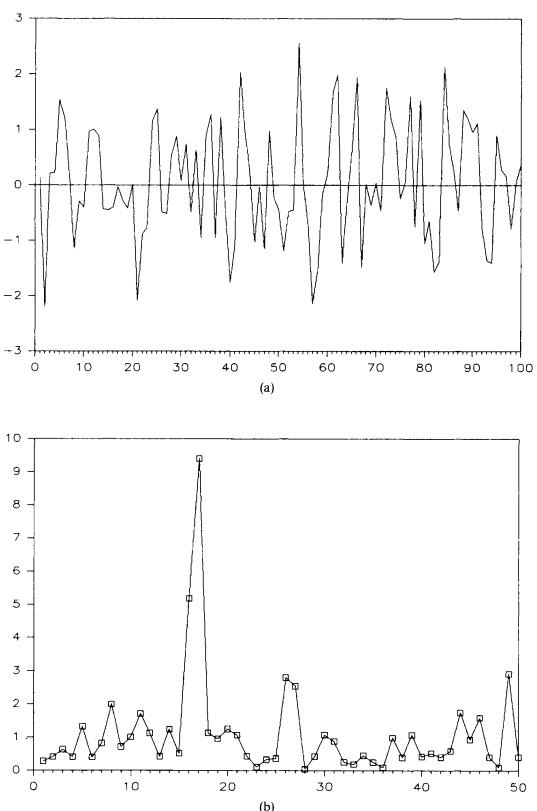
\includegraphics[height=0.5\textheight]{figures/04-periodogram-example.png}
  \caption{时间序列及其周期图。图片来自 \cite{brockwelldavis2006}, p.~340}
  \label{fig:ch4:periodogram}
\end{figure}

记
\[\begin{aligned} \bar{X}&:=\frac1n\sum_{t=1}^nX_i\\ \widehat\gamma(k)&:=\frac1n\sum_{t=1}^{n-|k|}(X_t-\bar{X})(X_{t+k}-\bar{X}) \end{aligned}\]
那么可以看出 $I_n(0)=n|\bar X|^2$ ；且当 $\omega_j\ne 0$ 时，

\begin{equation}
\label{eq:ch4:tag-8}
\begin{aligned} I_n(\omega_j)& = \frac1n\left|\sum_{t = 1}^{n}X_t e^{-it\omega_j}\right|^2\\ &=\frac1n\left|\sum_{t = 1}^{n}(X_t-\bar{X}) e^{-it\omega_j}\right|^2\\ &=\frac1n\sum_{t=1}^n\sum_{s=1}^n(X_t-\bar{X})(X_s-\bar{X})e^{-i(t-s)\omega_j}\\ &=\sum_{k=-(n-1)}^{n-1}e^{-ik\omega_j}\left(\frac1n\sum_{t=1}^{n-|k|}(X_t-\bar{X})(X_{t+|k|}-\bar{X})\right)\\ &=\sum_{|k|<n}\widehat\gamma(k)e^{-ik\omega_j} \end{aligned}
\end{equation}

接下来，我们把周期图延拓到 $[-\pi,\pi]$ 上：对任意 $\omega\in[-\pi,\pi]$ ，定义周期图为\[ I_n(\omega):=\begin{cases} I_n(\omega_k),&\text{ 若 }\omega_k-\frac\pi n<\omega\le \omega_k+\frac\pi n\text{ 且 }0\le\omega\le \pi\\ I_n(-\omega)&\text{ 若 }-\pi\le\omega<0 \end{cases} \]
即：在 $[0,\pi]$ 上，让 $I_n(\omega)$ 取值为最接近 $\omega$ 的那个 $\omega_k=\frac{2\pi j}{n}$ 的周期图；在 $[-\pi,0)$ 上直接对称过来；据此，可以构造一个映射 $g_n(\omega):[-\pi,\pi]\to \{2\pi j/n\}_{j=0,\pm1,\dots,\pm[n/2]}$ ，使得 $I_n(g_n(\omega))=I_n(\omega)$ 。

我们证明下述周期图的渐近性质：

\begin{theorem}[周期图的渐近无偏性]\label{thm:ch4:periodogram-expectation}

设 $\{X_t\}_{t\in\mathbb Z}$ 平稳，有均值为 $\mu$，且自协方差函数 $\gamma(\cdot)$ 绝对可和，则
\[\mathbb{E}[I_n(0)] - n\mu^2 \to 2\pi f(0) \quad \text{且} \quad \mathbb{E}[I_n(\omega)] \to 2\pi f(\omega) \quad \text{如果 } \omega \neq 0\]
如果 $\mu = 0$，则 $\mathbb{E}[I_n(\omega)]$ 在 $[-\pi, \pi]$ 上一致收敛到 $2\pi f(\omega)$。

\end{theorem}

\begin{proof}

首先，由定理~\ref{thm:ch4:long-run-variance}，
\[\mathbb{E}[I_n(0)] - n\mu^2 = n\mathbb{E}[|\bar{X}|^2] - n\mu^2 = n \mathrm{Var}(\bar{X}) = n \mathrm{Var}(S_n/n) \to \sum_{k=-\infty}^\infty \gamma(k) = 2\pi f(0)\]
现在如果 $\omega \in (0, \pi]$，则对充分大的 $n$，有 $g_n( \omega) \neq 0$。因此，由式~\eqref{eq:ch4:tag-8}，
\[\begin{aligned} \mathbb{E}[I_n(\omega)] &=\mathbb{E}[I_n(g_n(\omega))] \\ &=\sum_{|k|< n} \left(\frac1n\sum_{t = 1}^{n - |k|}\mathbb{E}[(X_{t} - \mu)(X_{t + |k|} - \mu)]\right)e^{-i k g_n(\omega)} \\ &= \sum_{|k|< n}\left(1 - \frac{|k|}{n}\right)\gamma (k)e^{-i k g_n(\omega)}  \end{aligned}\]
由于 $\gamma(\cdot)$ 绝对可和，级数 $\sum_{|k|< n}\left(1 - \frac{|k|}{n}\right)\gamma (k)e^{- i k\lambda}$ 在 $\lambda$ 上一致收敛到 $2\pi f(\lambda)$。因此，由于 $g_n(\omega) \to \omega$ 当 $n \to \infty$，我们有
\[\mathbb{E}[I_n(\omega)]\to 2\pi f(\omega)\]
当 $\mu = 0$ 时，利用 $f$ 在 $[-\pi,\pi]$ 上的一致连续性以及 $g_n(\omega)$ 在 $[0,\pi]$ 上一致收敛到 $\omega$ 可验证一致收敛性。

\end{proof}

定理~\ref{thm:ch4:periodogram-expectation} 的结论可以阐述为：若 $\omega\ne 0$，那么将 $\frac{I_n(\omega)}{2\pi}$ 作为 $f(\omega)$ 的估计量是渐近无偏的。

如果是线性过程，还有更精细的收敛结论，如下，

\begin{theorem}[周期图的有限维极限]
\label{thm:ch4:periodogram-limit}

令 $\{X_{t}\}_{t\in\mathbb Z}$ 为线性过程，满足 $X_{t} = \sum_{j = -\infty}^{\infty} \psi_j \epsilon_{t - j}$，其中 $\epsilon_{t}\sim F(0, \sigma^{2})$ i.i.d.，且 $\sum_{j = -\infty}^{\infty} |\psi_{j}| < \infty$。令 $I_{n}(\lambda)$ 表示 $\{X_{1}, \dots , X_{n}\}$ 的周期图， $f (\lambda)$ 为 $\{X_{t}\}_{t\in\mathbb Z}$ 的谱密度。

\begin{enumerate}
\def\labelenumi{\arabic{enumi}.}
\tightlist
\item
  如果对所有的 $\lambda \in [-\pi, \pi]$ 均有 $f(\lambda) > 0$，且 $0 < \lambda_{1} < \dots < \lambda_{m} < \pi$，则当 $n\to\infty$ 时随机向量 $(I_{n}(\lambda_{1}), \dots , I_{n}(\lambda_{m}))^{\top}$ 依分布收敛于一个随机向量，该向量的各个分量相互独立，且第 $i$ 个分量服从均值为 $2\pi f(\lambda_{i})$ 的指数分布。
\item
  如果进一步假设系数满足更强的衰减条件 $\sum_{j = -\infty}^{\infty} |\psi_{j}| |j|^{1/2} < \infty$，且 $\mathbb{E}[\epsilon_{1}^{4}] = \eta \sigma^{4} < \infty$，并令 $\omega_s = 2\pi s / n \geq 0$ 和 $\omega_t = 2\pi t / n \geq 0$ 为 Fourier 频率，则周期图在不同频率处的协方差具有如下精确的渐近展开：
  \[  \mathrm{Cov}(I_n(\omega_s), I_n(\omega_t)) = \begin{cases} 2(2\pi)^2 f^2(\omega_s) + O(n^{-1/2}) & \text{若 } \omega_s = \omega_t = 0 \text{ 或 } \pi, \\ (2\pi)^2 f^2(\omega_s) + O(n^{-1/2}) & \text{若 } 0 < \omega_s = \omega_t < \pi, \\ O(n^{-1}) & \text{若 } \omega_s \neq \omega_t. \end{cases}
  \]  其中，$O(n^{-1/2})$ 项与 $O(n^{-1})$ 项关于 $s$ 和 $t$ 是一致有界的。
\end{enumerate}

\end{theorem}

\begin{remark}

\begin{itemize}
\tightlist
\item
  定理~\ref{thm:ch4:periodogram-limit} 的证明见 \cite{brockwelldavis2006} 一书的 Theorem 10.3.2。除此之外，前文涉及的周期图相关结论和定理~\ref{thm:ch4:periodogram-expectation} 也见本书 Proposition 10.1.2、Proposition 10.3.1。
\item
  关于谱密度的估计，另一可参考的资料是 \cite{brillinger2001} 一书第 5 章。
\end{itemize}
\end{remark}

由定理~\ref{thm:ch4:periodogram-limit} 可见，如果我们用周期图 $\frac{I_n(\omega)}{2\pi}$ 来估计谱密度函数 $f(\omega)$，其方差不会随着样本量增加而消失，所以周期图 $\frac{I_n(\omega)}{2\pi}$ \emph{不是}谱密度的相合估计。这是我们不愿看到的：对参数 $\theta$，一个好的估计量 $\hat{\theta}_n$ 至少应当是相合的，即当 $n \to \infty$ 时，$\hat{\theta}_n$ 应依概率收敛到 $\theta$。

其原因在于：在经典的统计学中，样本量 $n$ 的增加通常意味着我们在同一个参数上获得了更多的独立观测，因此估计量的方差会以 $O(1/n)$ 下降；但在频域里，样本量 $n$ 的增加只是意味着我们在 $[-\pi, \pi]$ 上能分辨出更更多的点，而并没有在某一个特定的频率上增加重复观测。

然而有失有得：从定理~\ref{thm:ch4:periodogram-limit} 中还可以看到，当 $n$ 较大时且 $\omega_s\ne \omega_t$ 时，$\mathrm{Cov}(I_n(\omega_s), I_n(\omega_t))=O(n^{-1})\to 0$，说明周期图在各频率点上的纵坐标近似不相关；同时，由功率谱函数 $f(\lambda)$ 的连续性，在一个足够小的区间内，$I_n(\omega)$ 的方差也变化不大，因此我们有望通过在 $\lambda$ 的一个小邻域内对周期图纵坐标进行平均，来构造 $f(\lambda)$ 的相合估计量。本质上，这与经典统计中``通过样本平均消除随机误差以构造相合估计''是相同的。

\subsection{离散谱平均估计}

大多数传统方法采用的是一种称之为``周期图平滑''------或者叫``加窗''的方法，即用下述``\textbf{\emph{离散谱平均估计}} (discrete spectral average estimator)''：
\[
\widehat{f}(\omega_j)=\frac1{2\pi}\sum_{|k|\le m_n}W_n(k)I_n(\omega_{j+k}),
\]
作为谱密度的估计，其中 $W_n(\cdot)$ 满足

\begin{itemize}
\tightlist
\item
  当 $n\to\infty$ 时， $m_n\to\infty$ 但 $m_n/n\to 0$ ；
\item
  对每个 $k$ ， $W_n(k)=W_n(-k)$ ；
\item
  $\sum_{|k|\le m_n}W_n(k)=1$ ；
\item
  当 $n\to\infty$ 时， $\sum_{|k|\le m_n}W_n^2(k)\to 0$ 。
\end{itemize}

简而言之，我们用 $W_n(k)$ 作为权重，将 $-m_n\le k\le m_n$ 这段区域中的 $I_n(\omega_{j+k})$ 进行加权平均，以得到 $f(\omega_j)$ 的估计；这一过程如图~\ref{fig:ch4:spectral-smoothing} 所示。

\begin{figure}[htbp]
  \centering
  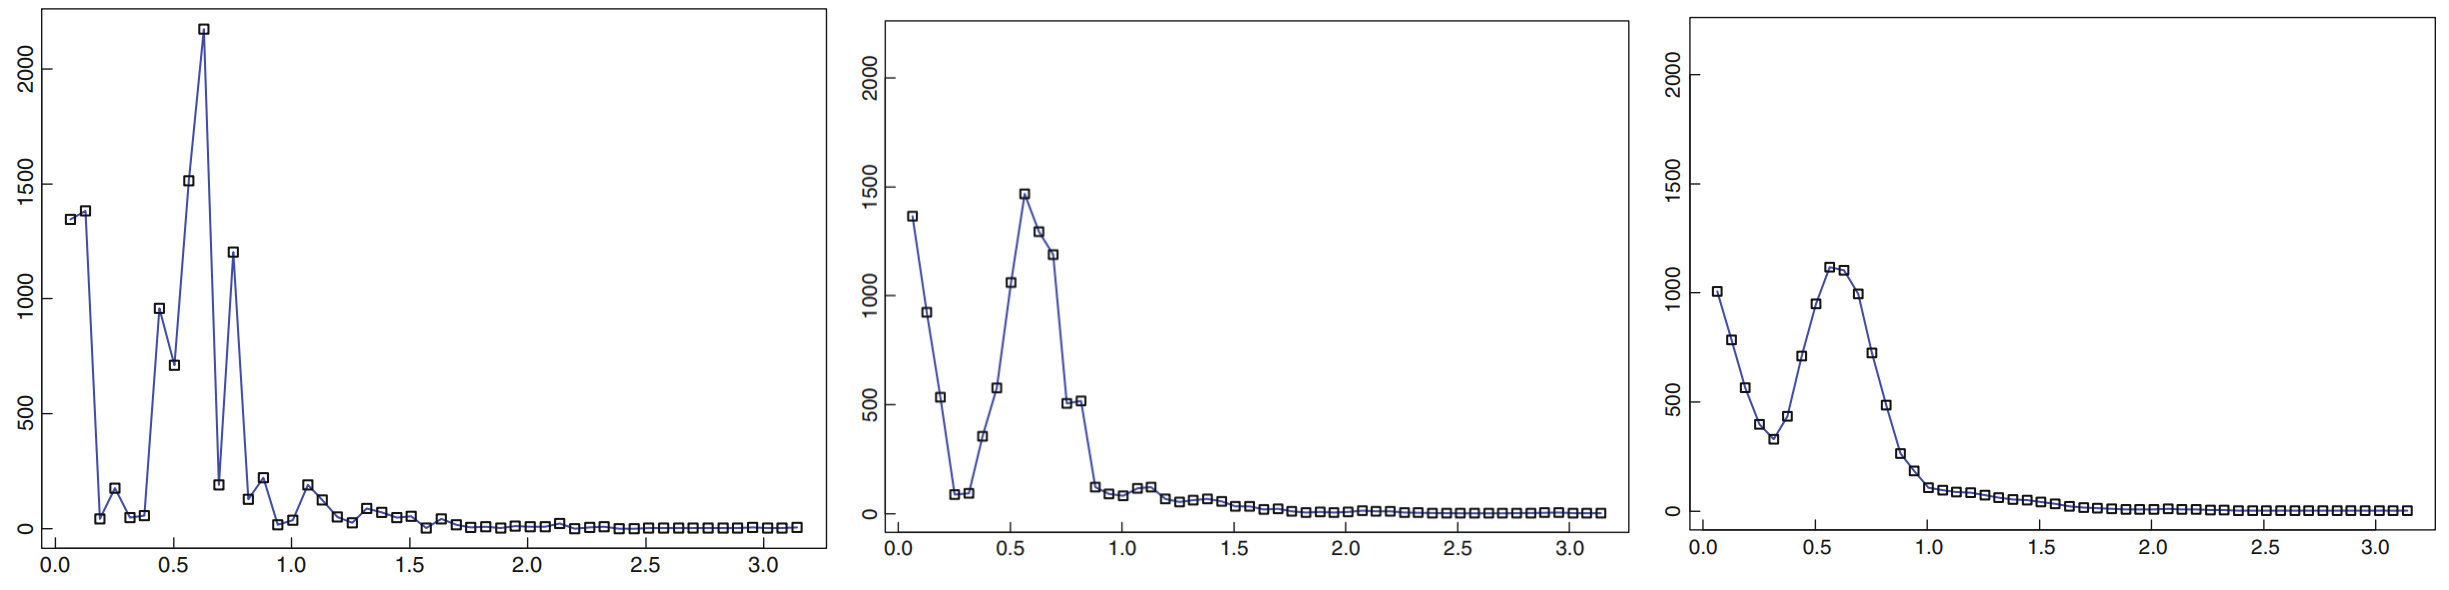
\includegraphics[width=0.96\textwidth]{figures/04-spectral-smoothing.png}
  \caption{离散谱平均估计的示意图。图片来自 \cite{brockwelldavis2006}, \S4.2}
  \label{fig:ch4:spectral-smoothing}
\end{figure}

类似于谱密度函数，用 $\widehat{f}(\omega)=\widehat f(g_n(\omega))$ 将 $\widehat f$ 延拓到 $[-\pi,\pi]$ 上。我们可以看到定理~\ref{thm:ch4:periodogram-limit} 的结果可以得到改进：

\begin{theorem}[离散谱平均估计的相合性]\label{thm:ch4:spectral-average-consistency}

令 $\{X_{t}\}_{t\in\mathbb Z}$ 为线性过程，满足 $X_{t} = \sum_{j = -\infty}^{\infty} \psi_j \epsilon_{t - j}$，其中 $\epsilon_{t}\sim F(0, \sigma^{2})$ i.i.d.，且 $\sum_{j = -\infty}^{\infty} |\psi_{j}| |j|^{1/2} < \infty$ ， $\mathbb{E}[\epsilon_1^4]<\infty$ 。那么谱平均估计 $\widehat f$ 满足：

\begin{itemize}
\tightlist
\item
  （渐近无偏）对 $\lambda\in[0,\pi]$ ， $\lim\limits_{n\to\infty}\mathbb{E}\big[\widehat f(\lambda)\big]=f(\lambda)$ ；
\item
  （相合性）对 $\omega_t,\omega_s\in[0,\pi]$，
  \[  \lim_{n \to \infty} \left( \sum_{|j| \leq m_n} W_n^2(j) \right)^{-1} \mathrm{Cov}\big[\widehat{f}(\omega_t), \widehat{f}(\omega_s)\big] = \begin{cases} 2f^2(\omega) & \text{ 若 } \omega_t = \omega_s = 0 \text{ 或 } \pi, \\ f^2(\omega) & \text{ 若 } 0 < \omega_t = \omega_s < \pi, \\ 0 & \text{ 若 } \omega_t \neq \omega_s. \end{cases}
  \]  这蕴含了 $\mathrm{Var}\big[\widehat f(\omega)\big]\sim f^2(\omega)\sum\limits_{|k|\le m_n}W_n^2(j)\to 0$ 。
\end{itemize}

\end{theorem}


见 \cite{brockwelldavis2006} 一书的 Theorem 10.4.1。

\subsection{非参数回归}

另一种思路称作``对数周期图回归''。注意到定理~\ref{thm:ch4:periodogram-limit} 导出了一个回归模型：
\[I_n(\omega_{j}) = (2\pi)f (\omega_{j})e_{j} + R_j,\quad j\in T\]
其中 $e_j\sim\mathrm{Exp}(1)$ i.i.d.，而 $R_j$ 是可忽略的项。（注意，根据定理~\ref{thm:ch4:periodogram-expectation}， $I_{n}(0)$ 可能是有偏的，如有必要我们从 $T$ 中剔除掉 $\{0\}$ ）。

将上式两边取对数，并忽略掉 $R_j$ ，
\[\log\left(\frac{I_{n}(\omega_j)}{2\pi}\right) = \log f (\omega_j) + \log e_j,\quad j\in T\]
这里 $\log e_j$ 服从 Gumbel 分布，有 $\mathbb{E}[\log(e_j)] = -0.57721\ldots$（Euler 常数），$\mathrm{Var}(\log(e_j)) = \pi^2 /6$。 令 $\eta_j := \log(e_j) + 0.57721\dots$，$W_j := \log(I_n(\omega_j) / (2\pi)) + 0.57721\ldots$，$m(\omega) := \log f(\omega)$，便得到如下固定设计 (fixed-design) 非参数回归模型：
\[W_{j} = m(\omega_{j}) + \eta_{j}, \quad j \in T\]
其中 $\{\eta_{j}\}$ i.i.d.，均值为零，方差 $\sigma_{\eta}^{2} = \pi^{2} / 6$。

我们可以通过``滑动平均''来估计 $m(0) = \log f(0)$。基于核函数 $K$ 和平滑带宽 (smoothing bandwidth) $b$ 的 $m(\omega)$ 的 \textbf{\emph{Nadaraya-Watson估计量 }} 为
\[\widehat{m}_b(\omega) = \frac{\sum_{j\in T } K\left(\frac{\omega - \omega_j}{b}\right) W_j}{\sum_{j\in T } K\left(\frac{\omega - \omega_j}{b}\right)}\]
其中当 $n\to\infty$ 时 $b \to 0$ 且 $nb \to \infty$ 。 最终，$f(0)$ 的估计量为 $\widehat{f}(0) = \exp(\widehat{m}_b(0))$。

\chapterreferences
\end{refsection}

\begin{refsection}
\extensionchapter{稳定分布与无限方差中心极限定理}{ext:stable-distributions}{E1}
% Generated from: Zhihu/专栏：概率与统计/稳定分布：方差无穷时的中心极限定理_金鱼马_2026-04-11.md
\section{极限分布}
回顾一下定义~\ref{def:ch1:limit-distribution} 对``极限分布" 的定义，简单起见我们只考虑一维的情况，
\begin{definition*}[极限分布]
若一列（一维）随机变量 $\{X_n\}$ 满足：存在常数数列 $a_n$、$b_n>0$ 和某个（非退化）分布 $F$，使得 $b_n^{-1}(X_n-a_n)\overset{\rm d}\to F$，
就称 $\{X_n\}$ 的\emph{极限分布} 或 \emph{渐近分布 }是 $F$ 。
\end{definition*}

% 这个概念可以推广到高维，只需把 $X_n$ 换成 $k$ 维随机向量、 $a_n$ 换成 $\mathbb R^k$ 中的向量、 $b_n$ 换成 $k\times k$ 正定矩阵即可，简单起见我们都只考虑一维的情况。

看了这个定义后，我们自然会问：怎么选择 $a_n\in\mathbb R$ 和 $b_n>0$ ，使得 $\frac{S_n-a_n}{b_n}\overset{\rm d}\to F$ ？如果使用不同的中心化和归一化参数 $a_n,b_n$ ，是否会收敛到不同的极限分布？答案是否定的，下面的定理~\ref{thm:ext-stable:convergence-types}说明：极限分布如果存在，它们总是``同一类''的。

首先，容易见到，若\[ b_n^{-1}(X_{n}-a_n)\overset{\rm d}\to Z\sim F(x) \]

那么对任意常数 $c>0$ 和 $d\in\mathbb R$，我们总可以通过取 $b_n'=cb_n$ 和 $a_n'=a_n+db_n$，使得
\[
b_n'^{-1}(X_{n}-a_n')=\frac1c(b_n^{-1}(X_n-a_n)-d) \overset{\text{d}}\to \frac1c(Z-d)\sim F(cx+d).
\]

故此，作为极限分布，我们总可以将 $F(x)$ 和 $F(cx+d)$ 视作是等效的。

\begin{definition*}[同型分布]
若两个分布函数 $F_1$ 和 $F_2$ 满足：存在常数 $c>0$ 和 $d$ 使得 $F_1(x)=F_2(cx+d)$ 对任意 $x$ 成立，那么称这两个分布 $F_1$ 和 $F_2$ 是\textbf{\emph{同一类的}} (of the same type)。
\end{definition*}

直观上，只要两个分布可以通过横坐标的拉伸/压缩（乘以常数 $c$）和左右平移（加上常数 $d$）完全重合，我们就认为它们拥有相同的``核心形状''。显见，这个``同一类''关系是一个等价关系，它将全体一维分布函数划分为一些互不相交的等价类。

\begin{theorem}[收敛型定理]
\label{thm:ext-stable:convergence-types}

设 $F,G$ 是两个 (非退化) 分布， $X_1,X_2,\dots$ 是随机变量，则，存在序列 $a_n\in\mathbb R$ 、 $b_n>0$ ，使得 $b_n^{-1}(X_n-a_n)\overset{\rm d}\to F$

并且又存在另一组序列 $a'_n\in\mathbb R$ 、 $b'_n>0$ ，使得 $b'^{-1}_n(X_n-a'_n)\overset{\rm d}\to G$

当且仅当存在 (唯一的) $c>0$ 和 $d$ 使得： \[ \lim_{n\to\infty}\frac{b'_n}{b_n}=c,\qquad \lim_{n\to\infty}\frac{a'_n-a_n}{b_n}=d \]于是， $F(x)=G(cx+d)$ ，说明 $F,G$ 是同一类的。

\end{theorem}
证明可见\cite{gnedenko1954}的第 2 章 §10。


\section{稳定分布}

上世纪二十年代，Lévy 提出了如下的概念，

\begin{definition*}[稳定分布]
一个分布 $F$ 被称为是\textbf{\emph{稳定}} (stable) 的，如果对于独立同分布于 $F$ 的 $X_1,X_2$ 以及 $X$，以及任意正数 $c_1,c_2$，总存在常数 $b>0$ 和 $a$，使得：
\[c_1 X_1 + c_2 X_2 \overset{\rm d}{=} b X + a\]
其中`` $\overset {\rm d}=$ ''代表同分布。直观来说，稳定分布对线性组合是``封闭''的，无论加多少个项，结果还是原来的分布形状，只是平移和缩放了。
\end{definition*}

\begin{remark}
这里 $a,b$ 依赖于 $c_1,c_2$。
\end{remark}

例如：

\begin{itemize}
\tightlist
\item
  正态分布显然是稳定分布，因为 $c_1X_1+c_2X_2\overset{\rm d}=\sqrt{c_1^2+c_2^2}X+\left(c_1+c_2-\sqrt{c_1^2+c_2^2}\right)\mu$ 。
\item
  Poisson 分布虽然也有可加性，但是它在线性组合下不封闭，因此不是稳定分布。
\end{itemize}

考虑 i.i.d. 同分布于某个稳定分布的随机变量之和 $S_n = X_1 + \cdots + X_n$。由定义，存在常数 $a_n \in \mathbb{R}$，$b_n > 0$ 以及 $X \overset{\rm d}{=} X_1$，使得对任意 $n=1,2,\dots$ ， \[ S_n = X_1 + X_2 + \cdots + X_n \overset{\rm d}{=} b_n X + a_n \quad \iff\quad b_n^{-1}(S_n - a_n) \overset{\rm d}{=} X \]所以稳定分布自身就可以作为 i.i.d. 和的一种极限分布。反过来也成立，所有可能的非退化极限分布也必是稳定的：

\begin{theorem}[稳定律的极限性质]
\label{thm:ext-stable:limit-property}

独立同分布随机变量通过适当归一化和中心化，得到所有可能 (非退化) 极限分布族，正是全体非退化稳定分布族。

\end{theorem}
证明可见\cite{gnedenko1954}的第 7 章 §33 (pp.~162-163)。


除正态、Cauchy、Lévy 分布外，绝大多数稳定分布没有解析形式的概率密度函数，但我们能通过特征函数来刻画它们，

\begin{theorem}[稳定律的谱表示]
\label{thm:ext-stable:spectral-representation}

设 $X$ 服从稳定分布，则其特征函数形如
\[\phi_X(t) = \mathbb{E}[e^{itX}] = \exp\big\{i\gamma t - c|t|^{\alpha}(1 - i\beta \operatorname{sign}(t)z(t, \alpha))\big\}, \quad t \in \mathbb{R}\]
其中 $\gamma$ 是实常数，$c > 0$，$\alpha \in (0, 2]$，$\beta \in [-1, 1]$，且\[ z(t, \alpha) = \begin{cases} \tan\left(\frac{\pi\alpha}{2}\right) & \text{若 } \alpha \neq 1, \\ -\frac{2}{\pi} \ln|t| & \text{若 } \alpha = 1\end{cases} \]

\end{theorem}
证明可见 \cite{ibragimov1971} 的 Theorem 2.2.2 (pp.43-45)、\cite{gnedenko1954} 的第 7 章 §34 等。


这里的有四个参数 $c,\gamma,\alpha,\beta$:

\begin{itemize}
\tightlist
\item
  $c$ 是尺度参数，控制分布的分散程度。$\gamma$ 是是位置参数。

\begin{itemize}
  \tightlist
  \item
    $c=0$ 对应于退化分布。
  \item
    这两个参数不用太关心，通过适当的线性变换，可以将任意稳定分布标准化为 $\gamma=0$ 、 $c=1$ 的形式。具体而言，对 $\alpha\ne1$ ，令 $Y=\frac{X-\gamma}{c^{1/\alpha}}$ ，则其特征函数为
    \[
    \phi_Y(t)=e^{-i\gamma t/c^{1/\alpha}}\phi_X(t/c^{1/\alpha}) = \exp\left\{ -|t|^\alpha \left(1 - i\beta \operatorname{sign}(t) \tan\left(\tfrac{\pi\alpha}{2}\right)\right) \right\}.
    \]
    对 $\alpha=1$ ，令 $Z=\tfrac{X-\gamma}{c}-\beta\tfrac2\pi\ln c$ ，则其特征函数为
    \[
    \phi_Z(t)=e^{-it\beta\frac2\pi\ln c}e^{-it\gamma/c}\phi_X(t/c)=\exp\big\{-|t|\left(1 - i\beta \operatorname{sign}(t)\tfrac2\pi\ln|t|\right)\big\}.
    \]
  \item
    后文中不失一般性地设 $\gamma=0$ 。
  \end{itemize}
\item
  $\alpha$ 是最重要的参数，它被称为\textbf{\emph{特征指数}} (characteristic exponent) 或者尾指数 (tail index)。

\begin{itemize}
  \tightlist
  \item
    它决定了分布的尾部厚度，继而也决定了矩的存在性等基本性质：当 $\alpha$ 减小时，分布中心变得更``尖''，而尾部则变得更厚。
  \item
    我们定义：特征指数为 $\alpha$ 的稳定分布称作 \textbf{\emph{α-稳定分布 }} (α-stable)，有时简记作``αs''。
  \end{itemize}
\item
  $\beta$ 是偏度参数，它控制分布的不对称性。

\begin{itemize}
  \tightlist
  \item
    当 $\beta = 0$ 时，分布关于位置参数对称，因为此时特征函数为 $e^{-c|t|^\alpha}$ 是实值函数； 当 $\beta > 0$ 时，分布向右偏斜； 当 $\beta < 0$ 时，分布向左偏斜。
  \item
    当 $\alpha=2$ 时， $\beta$ 不起作用：因为特征函数中的 $\beta$ 项乘以 $\tan(\pi\alpha/2)=\tan\pi=0$，无论 $\beta$ 取何值，特征函数都化为 $e^{-c t^2}$，对应正态分布。
  \item
    对称 α-稳定分布可以简记作``sαs''。
  \end{itemize}
\end{itemize}

图~\ref{fig:e1:stable-parameters} 就直观展示了 $\alpha,\beta$ 两个参数的作用：

\begin{figure}[htbp]
  \centering
  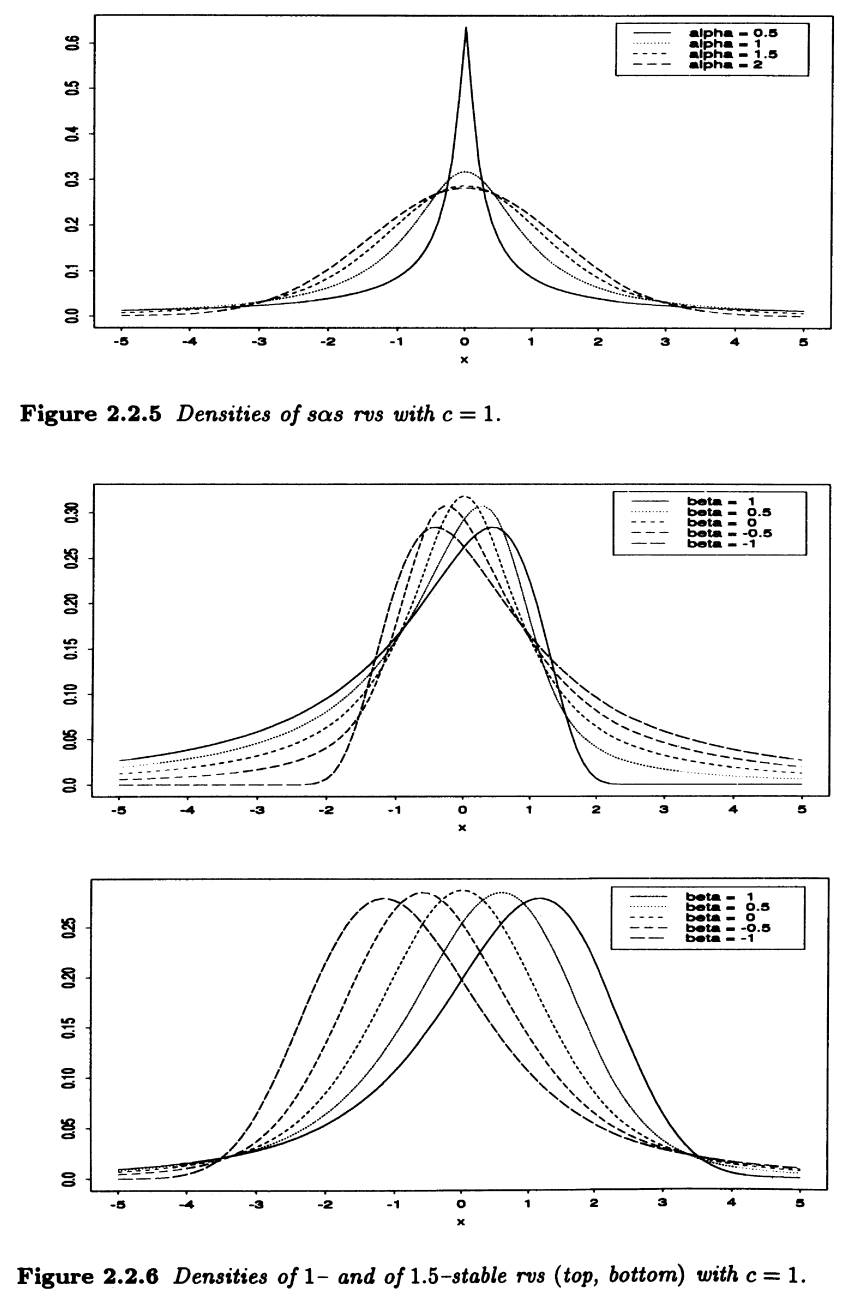
\includegraphics[height=0.68\textheight]{figures/e1-stable-parameters.png}
  \caption{稳定分布参数 $\alpha$ 与 $\beta$ 对分布形状的影响。图片来自 \cite{embrechts1997}, p.~73}
  \label{fig:e1:stable-parameters}
\end{figure}

稳定分布有非常多的应用。在金融数据、信号处理等各种领域的研究中 ，人们经常发现某些数据有 `` 高峰厚尾 '' 现象 ：数据不仅峰值高于正态分布，而且极端数据出现的频率也较大。此时用正态分布进行拟合显然是不当的，使用非正态的稳定分布来进行拟合，往往会更优。

\begin{example}[稳定分布的三个常见特例]

\begin{itemize}
\tightlist
\item
  取 $\alpha=2$ ，我们便得到了正态分布的特征函数 $e^{-ct^2}$ 。因此正态分布是一个 2-稳定分布。
\item
  取 $\alpha=1,\beta=0$ ，我们便得到了 Cauchy 分布的特征函数 $e^{-c|t|}$ 。因此 Cauchy 分布是 1-稳定分布。
\item
  若取 $\alpha=\frac12,\beta=1$ ，得到的是 \href{https://en.wikipedia.org/wiki/L\%C3\%A9vy_distribution}{Lévy 分布}，这是一个定义在正半轴上的右偏重尾分布，常用于描述 Brown 运动的首中时等。
\end{itemize}

这个例子表明，稳定分布是常见的正态分布、Cauchy 分布的推广。

虽然定理~\ref{thm:ext-stable:spectral-representation} 看起来很复杂，但事实表明，特征函数是能解析地刻画稳定分布的最好方式了 :-）对稳定分布进行统计推断的研究，基本都是从特征函数出发的，例如 \cite{feuerverger1981}、\cite{chan2009} 等。由于没有密度函数显式，因此对稳定分布的研究要困难一些，但人们还是通过很多方法得到了它的一些性质，例如，它的密度函数总是连续的，并且是单峰 (unimodal) 的；它的小于 $\alpha$ 阶矩存在，大于 $\alpha$ 阶矩不存在（见后文定理~\ref{thm:ext-stable:moments}）等。Zolotarev 的特征变换法，以及由DuMouchel 提出、Nolan 进一步发展的极大似然法\cite{nolan1997}都是稳定分布常用的估计方法。

\end{example}

\section{吸引域}

接下来的问题是，给定一个 α-稳定分布 $G_\alpha$ ，在何种条件下，随机变量的和 $S_n$ 经过适当归一化和中心化后，能收敛到 $G_\alpha$ ？

\begin{definition*}[吸引域]
设 $\{X_n\}_{n=1}^\infty$ i.i.d. 同分布于 $F$，且其部分和 $S_n$ 的极限分布是 $G_\alpha$，即存在常数 $a_n\in\mathbb R$、$b_n>0$，使得 $\frac{S_n-a_n}{b_n}\overset{\rm d}\to G_\alpha$，
那么，我们称 $F$ 属于 $G_\alpha$ 的\textbf{\emph{吸引域}} (Domain of attraction)。记作 $F \in \mathrm{DA}(G_\alpha)$。 如果只关心指数 $\alpha$，就简写为 $F \in \mathrm{DA}(\alpha)$。
\end{definition*}

下面的定理给出了完整的刻画，

\begin{definition*}[缓变函数]
$(0,\infty)$ 上（可测）的函数 $L(x)$ 若满足 $\lim_{x\to\infty}\frac{L(tx)}{L(x)}=1$，则称其为\textbf{\emph{缓变函数}} (slowly varying)。
\end{definition*}

缓变函数常见的例子是常函数和 $\ln x$ 、 $\ln\ln x$ 。

% \href{https://zhuanlan.zhihu.com/p/2024084738168603041}{【数学分析】缓慢变化函数与三个定理（一致收敛、karamata和potter上界）}

\begin{theorem}[吸引域的刻画]
\label{thm:ext-stable:domain-characterization}

\begin{itemize}
\tightlist
\item
  $\alpha = 2$ 的情形：$F \in \mathrm{DA}(2)$ 当且仅当 $\int_{|y| \le x} y^2 {\rm d}F(y)$是缓变的。
\item
  $\alpha < 2$ 的情形：$F \in \mathrm{DA}(\alpha)$（$\alpha < 2$）当且仅当存在缓变函数 $L(x)$ 以及非负常数 $c_1, c_2$（且 $c_1 + c_2 > 0$），使得\[ F(-x) = \frac{c_1 + o(1)}{x^\alpha} L(x), \quad 1 - F(x) = \frac{c_2 + o(1)}{x^\alpha} L(x), \quad x \to \infty \]
\end{itemize}

\end{theorem}

（证明见 \cite{gnedenko1954} 的第 7 章 §35，或者 \cite{ibragimov1971} 的 Theorem 2.6.1、Theorem 2.6.2。）


我们先来看第一条。若 $F$ 的二阶矩存在，那么 $L(x):=\int_{|y| \le x} y^2 {\rm d}F(y)$ 显然是一个缓变函数，因为无论是 $L(x)$ 还是 $L(tx)$ 在 $x\to\infty$ 时的极限都是 $\mathbb E[X^2],\,X\sim F$ 。所以定理~\ref{thm:ext-stable:domain-characterization} 推广了 Lindeberg--Lévy 中心极限定理。

但正态吸引域不仅限于有限二阶矩的情形。由于这两个条件是完全等价的：

\begin{itemize}
\tightlist
\item
  $\int_{|y| \le x} y^2 {\rm d}F(y)$ 是缓变函数；
\item
  $\lim\limits_{x\to\infty}\frac{x^2\int_{|y|>x}dF(y)}{L(x)} = 0$ ，即 $x^2\,P(|X|>x) = o\left(\int_{|y| \le x} y^2 {\rm d}F(y) \right)$ 。
\end{itemize}

所以定理第一条还有另一种叙述： $F$ 属于正态分布的吸引域，当且仅当

\begin{equation}
\label{eq:ext-stable:tag-1}
\frac{x^2\int_{|y|>x}\mathrm{d}F(y)}{\int_{|y|<x}y^2\mathrm{d}F(y)}\to 0\quad \text{ 当 }x\to\infty
\end{equation}

这实际上表明：就算二阶矩无穷大，尾部的质量要比``积分里的主项''小一个量级，可见正态分布的吸引域是非常广的。

再来看定理~\ref{thm:ext-stable:domain-characterization} 第二条，它表明 $\frac{F(-x)}{1-F(x)}\to \frac{c_1}{c_2}$，并且分布的左右尾部必须像 $x^{-\alpha}L(x)$ 那样衰减，换言之，$\frac{P(|X|>x)}{P(|X|>tx)}\sim t^\alpha$。相比于式~\eqref{eq:ext-stable:tag-1}，$\alpha<2$ 也有一种类似的形式：$F\in\mathrm{DA}(\alpha)$ 蕴含着存在缓变函数 $L(x)$ 使得，

\begin{equation}
\label{eq:ext-stable:tag-2}
P(|X|>x)=x^{-\alpha}L(x)
\end{equation}

且

\begin{equation}
\label{eq:ext-stable:tag-3}
\frac{x^2 P(|X| > x)}{\int_{|y|\le x} y^2 {\rm d}F(y)} \longrightarrow \frac{2 - \alpha}{\alpha}, \quad x \to \infty
\end{equation}

由式~\eqref{eq:ext-stable:tag-2} 可以看出，缓变函数 $L(x)$ 扮演着``尾部噪音''的角色；由式~\eqref{eq:ext-stable:tag-3} 可以看出，$\alpha<2$ 的 $\alpha$-稳定分布二阶矩必然为无穷（因为 $x^{2-\alpha}L(x)\to\infty$）。

进一步，我们可以得到矩的存在性结果：

\begin{theorem}[吸引域分布的矩]
\label{thm:ext-stable:moments}

若 $X\sim F \in \mathrm{DA}(\alpha)$，则：

\begin{itemize}
\tightlist
\item
  对 $0<\delta < \alpha$，$\mathbb E\big[|X|^\delta\big] < \infty$；
\item
  对 $\delta > \alpha$ 且 $\alpha < 2$，$\mathbb E\big[|X|^\delta\big] = \infty$。
\end{itemize}

特别地：

\begin{itemize}
\tightlist
\item
  当 $\alpha < 2$ 时， $\mathrm{Var}[X]=\infty$ ；
\item
  当 $\alpha > 1$ 时， $\mathbb{E}[|X|]<\infty$ ；
\item
  当 $\alpha < 1$ 时， $\mathbb{E}[|X|]=\infty$ 。
\end{itemize}

\end{theorem}

\begin{remark}

\begin{itemize}
\tightlist
\item
  定理~\ref{thm:ext-stable:moments} 第一条来自 B. V. Gnedenko，见\cite{gnedenko1954}的§35 Theorem 3 或者\cite{ibragimov1971}的 Theorem 2.6.4；第二条由式~\eqref{eq:ext-stable:tag-2} 可以直接看出。
\item
  若 $X\sim F\in\mathrm{DA}(\alpha)$ ，是可能存在 $\mathbb{E}[|X|^\alpha]<\infty$ 的。但是，若 $F$ 本身就是 $\alpha$ -稳定分布， $\alpha<2$ ，那么一定有 $\mathbb{E}[|X|^\alpha]=\infty$ 。
\end{itemize}
\end{remark}

\begin{example}[自由度为 2 的 $t$ 分布]
我们举一个简单的例子，自由度为 2 的 $t$ 分布 $t_2$ ，它的密度函数为 $f(x)=\frac1{(2+x^2)^{3/2}}$ ，容易验证其方差是不存在的：对 $X\sim t_2$ ，
\[\mathbb{E}[X^2]=\int_{\mathbb R}x^2\frac1{(2+x^2)^{3/2}}\mathrm{d}x=\infty\]
因此这个分布不满足传统 CLT 的条件。但是，我们能验证它位于正态分布的吸引域中，计算其尾部概率 \[ P(|X| > x) = 2 \int_x^\infty \frac{1}{(2+y^2)^{3/2}} \mathrm{d}y = 1 - \frac{x}{\sqrt{2+x^2}}=\frac1{x^2}+o\left(\frac1 {x^4}\right),\quad \text{ 当 }x\to\infty \]另一方面，根据 L'Hôpital 法则，
\[\lim_{n\to\infty}\frac{\int_0^x y^2f(y)\mathrm{d}y}{\ln x}=\lim_{n\to\infty}\frac{x^2f(x)}{1/x}=\lim_{n\to\infty}\frac{x^3}{(1+x^2)^{3/2}}=1\]
所以

\begin{equation}
\label{eq:ext-stable:tag-4}
\int_{|y|\le x}y^2f(y)\mathrm{d}y\sim 2\ln x
\end{equation}

由此可知，
\[
\frac{x^2P(|X|>x)}{\int_{|y|\le x}y^2f(y)\mathrm{d}y}\sim \frac{1}{2\ln x}\to 0.
\]
式~\eqref{eq:ext-stable:tag-1} 的条件满足！所以确实 $t_2\in\mathrm{DA}(2)$ 。可以证明，如果我们选择 $a_n=0$ 、 $b_n=\sqrt{n\ln n}$ ，那么
\[
\frac{S_n}{\sqrt{n\ln n}}\overset{\rm d}\to \mathcal N(0,1).
\]

这是一个``方差无限但仍然可以收敛到正态分布''的例子。


\end{example}

\section{归一化和中心化常数应该怎么选？}

\subsection{归一化常数}

首先，如果 $X$ 的分布是对称 $\alpha$ -稳定的，那么其特征函数为 $e^{-c|t|^\alpha}$ ，我们注意到
\[\begin{aligned} \phi_{n^{-1/\alpha}S_n}(t)&=\mathbb{E}[\exp \{itn^{-1/\alpha }S_n\}]\\ &=(\phi_X(n^{-1/\alpha }t))^n \\ &=\left(\exp\left\{-c|n^{-1/\alpha} t|^\alpha\right\}\right)^n\\ &=\exp\{-c|t|^\alpha\}\\ &=\phi_{X}(t) \end{aligned}\]
于是 $n^{-1/\alpha}S_n\overset{\rm d}=X$ 。所以直觉上 $b_n = n^{1/\alpha}$ 是合适的归一化项。

对于一般的吸引域中的 $X$，特征函数在 $0$ 附近的行为是 $\exp\{ -|t|^\alpha L_1(1/t) \}$，其中 $L_1$ 缓变（\cite{ibragimov1971} 的 Theorem 2.6.5），于是归一化项需要包含一个缓变修正：
\[b_n = n^{1/\alpha} L_2(n)\]
直观上，对于一个属于 $\mathrm{DA}(\alpha)$ 但不一定是稳定分布的 $X$，它的尾部可能不是纯幂律，而是 $P(|X|>x) \sim x^{-\alpha} L(x)$ （式~\eqref{eq:ext-stable:tag-3} ）。这时，若仍取 $b_n = n^{1/\alpha}$就不太够了，因为 $L$ 可能会把依分布收敛破坏掉；必须加上一个修正，从而将 $L(x)$ 的影响吸收掉。

为了更精确地构造 $b_n$，我们定义两个辅助函数：
\[K(x) := x^{-2} \int_{|y|\le x} y^2 {\rm d}F(y), \quad Q(x) := P(|X| > x) + K(x), \quad x > 0\]
那么，可以取 $b_n$ 为方程 $Q(b_n) = n^{-1}$ 的唯一解，或者渐近意义上是方程解。特别地，

\begin{itemize}
\tightlist
\item
  如果 $\sigma^2 = \mathrm{Var}[X] < \infty$ 且 $\mathbb E[X] = 0$，那么 $P(|X|>x)=o(x^{-2})$ 、 $K(x)=x^{-2}\mathbb{E}[X^2](1+o(1))$ 。此时若 $n^{-1}\sim Q(b_n)\sim b_n^{-1}\sigma^2$ ，我们可以直接选取 $b_n =n^{1/2} \sigma$。
\item
  如果 $\alpha < 2$，我们可以取 $b_n = \inf\{ y : P(|X| > y) < n^{-1} \}$，此时 $P(|X| > b_n) \sim n^{-1}$，并且 式~\eqref{eq:ext-stable:tag-2}告诉我们 $b_n = n^{1/\alpha} L_3(n)$，$L_3$ 缓变。 那么，根据式~\eqref{eq:ext-stable:tag-3} ， $K(x) \sim \frac{\alpha}{2-\alpha}P(|X|>x)$ ，于是\[ Q(x) = P(|X|>x)+ K(x) \sim \left(1 + \frac{\alpha}{2-\alpha}\right) P(|X|>x) = \frac{2}{2-\alpha} P(|X|>x) \] 即 $Q(x)$ 与 $P(|X|>x)$ 相差一个常数倍， $P(|X| > b_n) \sim n^{-1}$ 已经足够。
\end{itemize}

为什么要让 $Q(b_n)\sim n^{-1}$ 呢？直观上，对于重尾分布，和 $S_n$ 的渐近行为由两部分共同决定：

\begin{itemize}
\tightlist
\item
  ``大量微小震荡''（$|X_i| \le b_n$）：这部分累积的方差贡献由 $K(x)$ 描述。
\item
  ``单次巨大跳跃''（$|X_i| > b_n$）：这部分由 $P(|X|>x)$ 描述。
\end{itemize}

如果我们希望标准化后的和 $\frac{S_n - a_n}{b_n}$ 收敛到某个非退化极限分布，就需要让上述两种贡献加起来后的总波动能在尺度 $b_n$ 下得以被控制，这就是让 $nP(|X|>b_n)+nK(b_n)=nQ(b_n)=1$ 的含义。

% （当然这个只是直觉上的解释，理论上应该也是可以进行推导的。）

读者可以看图~\ref{fig:e1:partial-sum-paths}，对于标准正态分布， $S_n$ 总体上是比较连续的；而对于诸如标准 Cauchy 这样的重尾分布，由于极端值更可能出现， $S_n$ 会产生比较大的跳跃：

\begin{figure}[htbp]
  \centering
  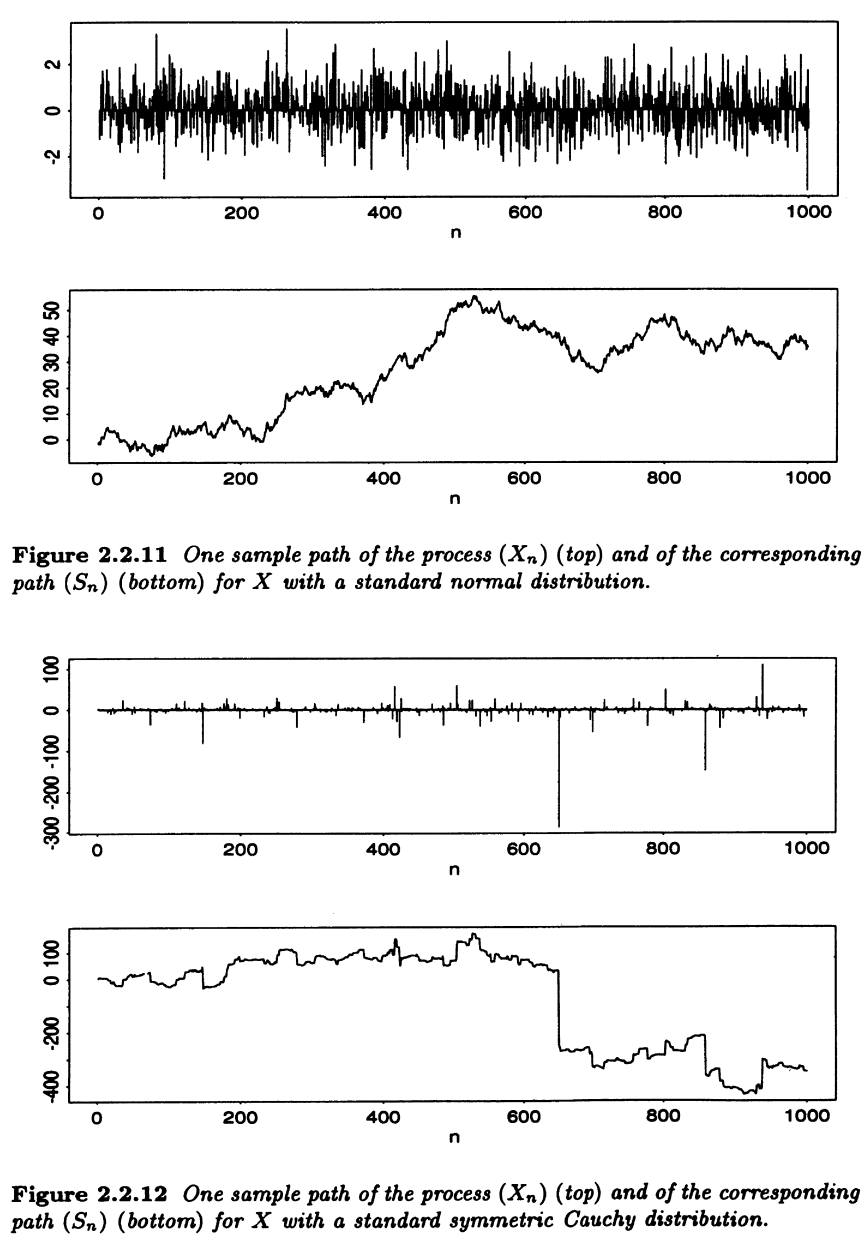
\includegraphics[height=0.68\textheight]{figures/e1-partial-sum-paths.png}
  \caption{正态分布与重尾分布的部分和路径。图片来自 \cite{embrechts1997}, p.~77}
  \label{fig:e1:partial-sum-paths}
\end{figure}

这背后隐含着重尾分布的一个核心直觉：``单次大跳跃原理 (Single Big Jump Principle)''。在经典的正态中心极限定理中，和 $S_n$ 的波动是由大量微小的独立震荡累积而成的；但在 Cauchy 等重尾分布中，和 $S_n$ 的极端波动往往是由某一个或极少数几个极端的观测值主导的。

\begin{example}[$t_2$ 分布的归一化常数]
继续前文的 $t_2$ 分布。式~\eqref{eq:ext-stable:tag-1} 告诉我们 $P(|X|>x)/K(x)\to 0$ ，因此 $Q(x)=P(|X|>x)+K(x)\sim K(x)$ 。式~\eqref{eq:ext-stable:tag-4} 告诉我们 $K(x)\sim \frac{2\ln x}{x^2}$ ，于是方程 $Q(b_n)\sim K(b_n)\sim n^{-1}$ 化作 $b_n^2\sim 2n\ln b_n$ ，容易看出 $b_n=\sqrt{n\ln n}$ 是满足的。

\end{example}


\subsection{中心化常数}

中心化常数 $a_n$ 的选择是下述截断均值： $a_n=n\int_{|y|\le b_n}y\mathrm{d}F(y)$或者渐近意义上使得上式成立；其中 $b_n$ 由上节的方法确定。之所以要用截断均值，是因为总体均值 $\mathbb{E}[X]$ 在 $\alpha\le 1$ 时是不存在的，不能简单地用 $n\mathbb {E}[X]$ 来中心化，我们只能退而求其次，对那些``不太大''（ $|y|\le b_n$ ）的项进行中心化对齐。

\begin{itemize}
\tightlist
\item
  不过，一种简单的情形是，如果分布是对称的，例如关于 0 对称，我们可以直接取 $a_n=0$ 。
\item
  对 $1<\alpha\le 2$ 的情况，由于均值 $\mu$ 存在且 $\int_{|y|\le b_n}y\mathrm{d}F(y)\to \mu$ ，我们取 $a_n=n\mu$ 即可。
\end{itemize}

\section{广义中心极限定理}

把上面所有的准备工作合并起来，我们就得到了最完整的结论：

\begin{theorem}[广义中心极限定理]
\label{thm:ext-stable:gclt}

设 $F \in \mathrm{DA}(\alpha)$，$\alpha \in (0,2]$。

\begin{itemize}
\tightlist
\item
  二阶矩有限情形（此时必有 $\alpha=2$ ）：如果 $\mathbb{E}[X^2]<\infty$ ，则
  \[
  \frac{S_n - n\mu }{\sigma n^{1/2}} \overset{\rm d}\to \mathcal N(0,1).
  \]
\item
  如果 $\mathbb E[X^2] = \infty$ 且 $\alpha = 2$，或者 $\alpha < 2$，那么存在缓变函数 $L_4(n)$ 和 (上节中定义的) 序列 $a_n$，使得
  \[
  \frac{S_n-a_n}{n^{1/\alpha}L_4(n)}\overset{\rm d}\to G_\alpha,
  \]
  其中 $G_\alpha$ 是一个 $\alpha$-稳定分布。
\end{itemize}

\end{theorem}

在某些特殊情况下，归一化常数 $b_n=n^{1/\alpha}L_4(n)$ 中的缓变函数 $L_4(n)$ 可以吸收为一个常数，即 $b_n = c n^{1/\alpha}$。这时我们称分布属于 \textbf{\emph{正规吸引域}} (domain of normal attraction)。

\begin{definition*}[正规吸引域]
如果分布 $F\in\mathrm{DA}(G_\alpha)$ 且可以选取 $b_n=cn^{1/\alpha}$（$c>0$ 为常数）使得 $\frac{S_n-a_n}{b_n}\overset{\rm d}\to G_\alpha$ 成立，则称 $F$ 属于 $G_\alpha$ 的\textbf{\emph{正规吸引域}}，记作 $F\in\mathrm{DNA}(G_\alpha)$ 或 $F\in\mathrm{DNA}(\alpha)$。
\end{definition*}

根据我们前文对归一化常数选取的分析，以及定理~\ref{thm:ext-stable:domain-characterization}，推知

\begin{theorem}[正规吸引域的刻画]
\label{thm:ext-stable:normal-domain-characterization}

\begin{itemize}
\tightlist
\item
  当 $\alpha = 2$ 时：$F \in \mathrm{DNA}(2)$ 当且仅当 $\mathbb E[X^2] < \infty$。
\item
  当 $\alpha < 2$ 时：$F \in \mathrm{DNA}(\alpha)$ 当且仅当存在非负常数 $c_1, c_2$（$c_1 + c_2 > 0$）使得
  \[
  F(-x) \sim c_1 x^{-\alpha}, \quad 1 - F(x) \sim c_2 x^{-\alpha}, \quad x \to \infty.
  \]
\end{itemize}

\end{theorem}

也就是说，正规吸引域中，分布的尾部是纯幂律的，不需要缓变函数进行修正。特别地，所有 $\alpha$ -稳定分布都在它自己的正规吸引域中。
 

\nocite{embrechts1997,gnedenko1954,ibragimov1971}
\chapterreferences
\end{refsection}

\begin{refsection}
\extensionchapter{泛函中心极限定理}{ext:functional-clt}{E2}
% Generated from: Zhihu/专栏：概率与统计/泛函中心极限定理：从 Brown 运动到 α‑稳定过程_金鱼马_2026-04-09.md
\section{基本概念和准备}

\subsection{两种随机函数的构造}

如何把 $S_n$ ``视作随机函数''呢？具体来说，我们要做的是将其视作 $[0,1]$ 上的连续时间随机过程 $S_n(\cdot)$。这便需要对时间轴和空间尺度同时进行变换。

最简单的做法是，在离散时间点 $t = k/n$（$k = 0,1,\dots,n$）处，定义
\[S_n\Bigl(\frac{k}{n}\Bigr) = \frac{1}{\sigma\sqrt{n}} \bigl( S_k - \mu k \bigr).\]
然后，对于任意的 $t \in [0,1]$，用直线接相邻的点 $(k/n, S_n(k/n))$ 和 $((k+1)/n, S_n((k+1)/n))$。显式写出来就是
\[S_n(t)=\frac{1}{\sigma\sqrt{n}}  \Bigl(S_{[nt]}-\mu [nt]+(nt-[nt])(X_{[nt]+1}-\mu)\Bigr)\]
其中 $[nt]$ 表示 $nt$ 的整数部分。这样得到的 $S_n(t)$ 是一个连续的折线函数，其样本路径属于连续函数空间 $\mathcal{C}[0,1]$。换言之，$S_n$ 定义了一个从概率空间到连续函数空间的随机变量（或者称随机函数）：
\[\begin{array}{ccl} S_n: & (\Omega,\mathscr F, P)&\to \mathcal C[0,1]\\ & \omega &\mapsto  S_n(\cdot,\omega) \end{array}\]
我们称 $\{S_n(t)\}_{n=1}^\infty$ 是由随机变量 $\{X_n\}_{n=1}^\infty$ 产生的\emph{部分和过程序列}。

传统中心极限定理的目标是考察部分和 $S_n$ 在 $(\mathbb R,\mathcal B_{\mathbb R})$ 中的弱收敛性；而面对部分和过程序列 $\{S_n(t)\}_{n=1}^\infty$，我们的目标便是研究它在 $\mathcal C[0,1]$ 中的弱收敛性。注意，这里我们要为连续函数空间 $\mathcal C[0,1]$赋予上确界范数
\[\|x\|_\infty = \sup_{0\le t\le 1}|x(t)|\]
及其生成的 Borel $\sigma$-代数 $\mathscr C$ ；此时在度量 \[ \rho(x,y):=\|x-y\|_\infty=\sup\limits_{0\le t\le 1}|x(t)-y(t)| \]下的收敛对应了一致收敛，称 $\rho$ 为一致收敛度量，其诱导的拓扑为一致收敛拓扑。

另一种更简单的构造是
\[\widetilde S_n(t) = \frac{1}{\sigma\sqrt{n}} \bigl( S_{[nt]} - \mu [nt] \bigr), \qquad 0 \le t \le 1,\]
这个函数在区间 $[k/n, (k+1)/n)$ 上为常数，在 $t = k/n$ 处可能有跳跃。因此它的样本路径是\emph{右连左极}的。

\begin{definition*}[右连左极函数]
设 $(M,d)$ 是度量空间，$E\subset\mathbb R$。若函数 $f:E\to M$ 满足：

\begin{itemize}
\tightlist
\item
  右连续：$f(t+)=\lim\limits_{s\to t^+} f(s)$ 存在，且等于 $f(t)$;
\item
  左极限：$f(t-)=\lim\limits_{s\to t^-} f(s)$ 存在且有限。
\end{itemize}

那么称 $f$ 是``右连续且存在左极限'' 的，简称``\textbf{\emph{右连左极}}''。法文称为 \textbf{\emph{\href{https://en.wikipedia.org/wiki/C\%C3\%A0dl\%C3\%A0g}{Càdlàg}}} （continue à droite, limite à gauche）。
\end{definition*}

我们将 $[0,1]$ 上全体``右连左极''的实值函数构成的集合记作 $\mathcal D[0,1]$。显然

\begin{itemize}
\tightlist
\item
  $\mathcal D[0,1]$ 中所有函数的间断点都是第一类间断点；
\item
  $\mathcal D[0,1]\supset \mathcal C[0,1]$ 。
\end{itemize}

同样在 $\mathcal D[0,1]$ 中赋予上确界范数及其生成的 Borel $\sigma$-代数。

显然，$\widetilde S_n(t)$ 与 $S_n(t)$ 在分点 $k/n$ 处取值相同，但前者是阶梯函数，后者是折线。当 $n$ 很大时，两者在视觉上非常接近，直觉上二者应该有同样的收敛性结论。

\subsection{Brown 运动}

\begin{definition*}[标准 Brown 运动]
$[0,1]$ 上的实值随机过程 $B(t)$ 如果满足以下四个条件：

\begin{enumerate}
\def\labelenumi{\arabic{enumi}.}
\tightlist
\item
  \emph{起点为零}：$B(0) = 0$ a.s.。
\item
  \emph{独立增量}：对任意 $0 \le t_0 < t_1 < \dots < t_m \le 1$，增量 $B(t_1)-B(t_0), \dots, B(t_m)-B(t_{m-1})$ 相互独立。
\item
  \emph{增量正态性}：对每个 $s,t \in [0,1]$，$t\ge s$，$B(t)-B(s) \sim N(0, t-s)$。
\item
  \emph{路径连续性}：样本路径 $t \mapsto B(t)$ a.s. 连续。
\end{enumerate}

则称 $B(t)$ 为标准 \textbf{\emph{\href{https://en.wikipedia.org/wiki/Brownian_motion}{Brown 运动}}} （或 Wiener 过程）。它也可以视作将概率空间 (a.s. 地) 映射到 $\mathcal C[0,1]$ 的随机函数：
\[\begin{array}{ccl} B: & (\Omega,\mathscr F, P)&\to \mathcal C[0,1]\\ & \omega &\mapsto  B(\cdot,\omega) \end{array}\]\end{definition*}

图~\ref{fig:e2:brownian-paths} 展示了标准 Brown 运动的若干条样本轨迹。

\begin{figure}[htbp]
  \centering
  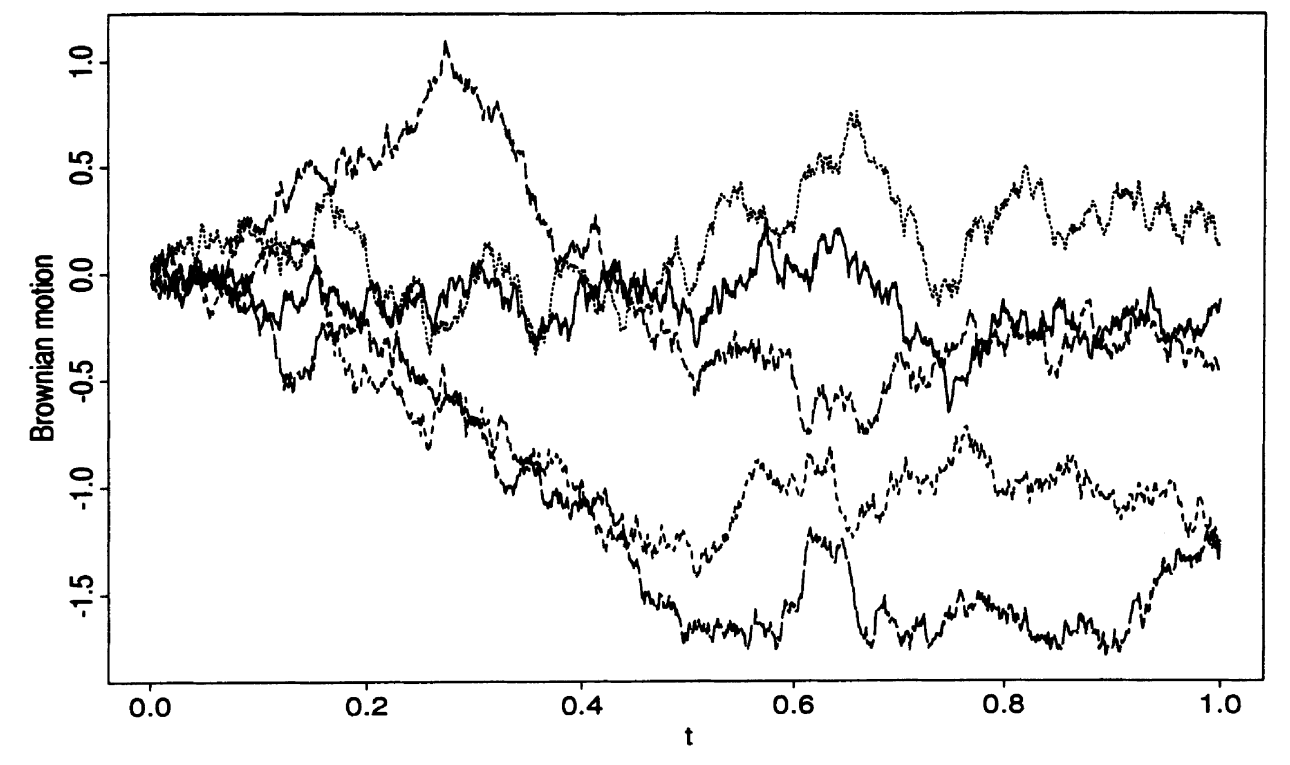
\includegraphics[width=0.88\textwidth]{figures/e2-brownian-paths.png}
  \caption{$[0,1]$ 上标准 Brown 运动的五条样本轨迹。图片来自 \cite{embrechts1997}, p.~89}
  \label{fig:e2:brownian-paths}
\end{figure}

Brown 运动是概率论中最重要的随机过程之一，其存在性和构造、以及相关的性质（样本路径 Hölder 连续、几乎处处不可微、变差无界等等）和理论等，我们在此不必多提，随便一本教材上都会讲解。在这里，我们要用标准 Brown 运动替代经典中心极限定理中的正态分布 $\mathcal N(0,1)$，扮演``极限过程''的核心角色。

\subsection{度量空间中的弱收敛}

回顾弱收敛的定义~\ref{def:ch1:weak-convergence}：设 $(S, \rho)$ 是一个度量空间（$\rho$ 是距离函数），并赋予其 Borel $\sigma$-代数（由所有开集生成）。令 $X, X_1, X_2, \dots$ 是取值于 $S$ 的随机元。如果对任意有界、连续的实值函数 $f: S \to \mathbb{R}$，都有
\[\lim_{n\to\infty}\mathbb{E}[f(X_n)]=\mathbb{E}[f(X)]\]
称序列 ${X_n}$ 弱收敛 于 $X$（记作 $X_n \overset{\rm d}\to X$）。当 $S = \mathbb{R}$ 且 $\rho$ 是通常绝对值距离时，上述定义就退化为经典的随机变量弱收敛，即，依分布收敛。
当然，我们面临的空间 $S$ 是 $\mathcal C[0,1]$ 或者 $\mathcal D[0,1]$ ，在证明依分布收敛时，上面这个``用有界连续函数刻画''的标准定义总是不太方便。更具有操作性的框架是借助 Prokhorov 定理（定理~\ref{thm:ch1:prohorov}），将弱收敛拆解为``有限维分布的收敛''加上``相对紧性（由一致胎紧性保证）''。
% \begin{definition*}[胎紧]
% 取值于度量空间 $S$ 上的一族随机变量 $\{X_\pi\}_{\pi\in\Pi}$ 如果满足：对任意 $\epsilon>0$，有紧集 $K\subset S$，使得 $\sup\limits_{\pi\in\Pi}P(X_\pi\notin K)<\epsilon$，则称这族随机变量是\textbf{\emph{胎紧}} (tight) 的。简而言之，胎紧意味着一族随机变量一致地集中在一个紧集上。
% \end{definition*}
% \begin{theorem}[Prokhorov 定理]
% \label{thm:ext-fclt:prokhorov}
% 若取值于度量空间 $S$ 上的一族随机变量 $\{X_\pi\}_{\pi\in\Pi}$ 是一致胎紧的，则其是 (弱) \textbf{\emph{相对紧}} 的，即，其中的任意序列 $\{X_{n}\}_{n=1}^\infty$ 有弱收敛的子列。反过来，若 $S$ 是可分完备度量空间，那么 $S$ 上的概率测度族相对紧蕴含一致列紧。
% \end{theorem}
在 $(\mathcal C[0,1],\rho)$ 中，有限维柱集构成了\emph{确定类} (determining class / separating class)。简而言之，这是说，对于取值于 $\mathcal C[0,1]$ 的随机元，如果我们能确定它的所有有限维分布，即，对任意 $0\le t_1<\cdots<t_m\le 1$ ，我们能确定 $(X(t_1),\dots,X(t_m))$ 的分布，就可以确定 $X$ 本身的分布 (e.g., 见 \url{https://math.stackexchange.com/q/3450060})；这一结论单独还不足以确定收敛性，但只要与 Prokhorov 定理结合起来，便能得到

\begin{corollary}\label{cor:ext-fclt:finite-dimensional-tightness}
设 $X_n$ 和 $X$ 是取值于 $(\mathcal C[0,1],\rho)$ 的随机变量，$X_n\overset{\rm d}\to X$ 当且仅当如下两个条件成立：

\begin{itemize}
\tightlist
\item
  $\{X_n\}_{n=1}^\infty$ 一致胎紧；
\item
  对任意 $0\le t_1<\cdots<t_m\le 1$ ，有 $(X_n(t_1),\dots,X_n(t_m))\overset{\rm d}\to (X(t_1),\dots,X(t_m))$ 。
\end{itemize}
\end{corollary}

这个结论对后文要介绍到的 Skorokhod 度量 $(\mathcal D[0,1],d_0)$ 也是成立的。

\section{Donsker 定理}

所谓``泛函中心极限定理 (FCLT)''，确切来说叫 \textbf{\emph{Donsker 定理}} ，得名于 Monroe D. Donsker。其叙述如下：

\begin{theorem}

Donsker 定理：设 $X_1, X_2, \dots$ i.i.d.，$\mathbb{E}[X_1] = \mu$，$0 < \mathrm{Var}[X_1] = \sigma^2 < \infty$。则

\begin{itemize}
\tightlist
\item
  在 $(\mathcal{C}[0,1],\rho)$ 中，有 \[S_n(\cdot) \overset{\rm d}\to B({\cdot})\]\item
  在 $(\mathcal{D}[0,1],\rho)$ 中，有 \[\widetilde S_n(\cdot) \overset{\rm d}\to B(\cdot)\]\end{itemize}
\end{theorem}

该定理又称``Donsker 不变原理''，强调了极限过程与 $X_n$ 的具体分布无关 ------ 只要方差有限，其随机游走路径总是收敛到 Brown 运动。它是一个非常强大的结果。

我们这里不具体介绍其证明（因为比较繁琐）。非常简略来说，完整的证明需要两大部分：

\begin{enumerate}
\def\labelenumi{\arabic{enumi}.}
\tightlist
\item
  有限维分布收敛：对任意 $0 \le t_1 < \dots < t_m \le 1$，向量 $(S_n(t_1), \dots, S_n(t_m))$ 依分布收敛到 $(B(t_1), \dots, B(t_m))$。这需要用到独立增量性质。
\item
  胎紧性：证明序列 $\{S_n(\cdot)\}$ 在 $\mathcal{C}[0,1]$ 中是胎紧的。通常需要验证 \emph{一致连续性模} 的收敛：对任意 $\epsilon > 0$，
  \[
  \lim_{\delta \to 0} \limsup_{n\to\infty} P\Bigl( \sup_{|t-s|<\delta} |S_n(t)-S_n(s)| > \epsilon \Bigr) = 0.
  \]
\end{enumerate}

那么由上节推论，这两个条件等价于弱收敛。这个是 Billingsley 的经典证明。至于 $(\mathcal{D}[0,1],\rho)$ 的情形，证明要借助后文将介绍的 Skorokhod 拓扑。

图~\ref{fig:e2:donsker-convergence} 是 Donsker 定理的示意图。可以看到，随着 $n$ 逐渐增加， $S_n(\cdot)$ 越来越趋近于 Brown 运动的样本路径。

\begin{figure}[htbp]
  \centering
  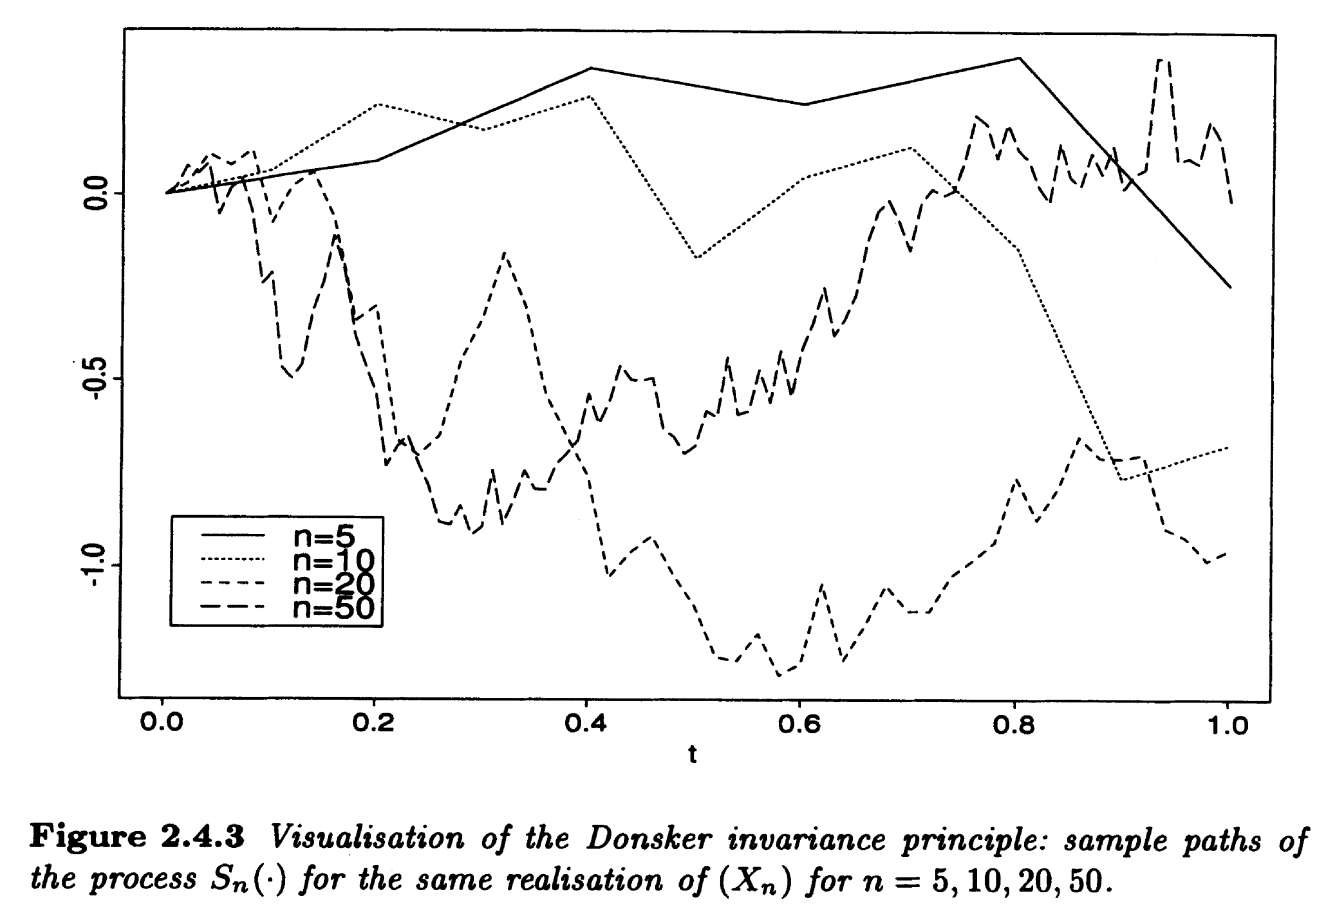
\includegraphics[width=0.88\textwidth]{figures/e2-donsker-convergence.png}
  \caption{Donsker 定理的示意图。图片来自 \cite{embrechts1997}, p.~90}
  \label{fig:e2:donsker-convergence}
\end{figure}

Donsker 定理可以配合连续映射定理 (定理~\ref{thm:ch1:continuous-mapping}) 来使用：


在 $\mathcal{C}[0,1]$ 或 $\mathcal{D}[0,1]$ 上，以下泛函在 $\rho$ 下是连续的：

\begin{itemize}
\tightlist
\item
  取值泛函：$f_1(x) = x(1)$。
\item
  最大值：$f_2(x) = \sup_{0\le t\le 1} x(t)$。
\item
  最小值：$f_3(x) = \inf_{0\le t\le 1} x(t)$。
\item
  振幅：$f_4(x) = \sup_t x(t) - \inf_t x(t)$。
\item
  积分：$f_5(x) = \int_0^1 x(t)\,\mathrm dt$。
\end{itemize}

利用 Donsker 定理和连续映射定理，我们立刻得到许多有用的收敛结果。

\begin{example}[Donsker 定理的连续泛函]
以 $f_1$、$f_2$、$f_3$ 为例，注意到
\[
\begin{aligned}
f_1(S(\cdot))=f_1(\widetilde S(\cdot))
  &=\frac{S_n-n\mu}{\sigma\sqrt n},\\
f_2(S(\cdot))=f_2(\widetilde S(\cdot))
  &=\frac1{\sigma\sqrt n}\max_{0\le k\le n}(S_k-k\mu),\\
f_3(S(\cdot))=f_3(\widetilde S(\cdot))
  &=\frac1{\sigma\sqrt n}\min_{0\le k\le n}(S_k-k\mu).
\end{aligned}
\]
那么
\[\begin{aligned} \frac{1}{\sigma\sqrt{n}} (S_n - n\mu) &\overset{\rm d}\to B(1)\overset{\rm d}=\mathcal N(0,1)\\ \frac{1}{\sigma\sqrt{n}} \max_{0\le k\le n} (S_k - k\mu) &\overset{\rm d}\to \sup_{0\le t\le 1} B(t)\\ \frac{1}{\sigma\sqrt{n}} \min_{0\le k\le n} (S_k - k\mu) &\overset{\rm d}\to \inf_{0\le t\le 1} B(t) \end{aligned}\]
更一般地，联合分布也收敛：
\[\Bigl( \frac{S_n - n\mu}{\sigma\sqrt{n}},\; \frac{\max_{k}(S_k - k\mu)}{\sigma\sqrt{n}},\; \frac{\min_{k}(S_k - k\mu)}{\sigma\sqrt{n}} \Bigr) \overset{\rm d}\to \bigl( B_1,\; \sup B(t),\; \inf B(t) \bigr)\]
\end{example}

\begin{example}[有限维分布]
取 $0\le t_1<\dots<t_m\le 1$，考虑 $\mathcal C[0,1]$ 上的泛函 $x\mapsto (x(t_1),\dots,x(t_m))$。该映射在 $\mathcal C[0,1]$ 上处处连续，因此
\[\bigl( S_n(t_1),\dots,S_n(t_m) \bigr) \overset{\rm d}\to (B(t_1),\dots,B(t_m)).\]
这表明 Donsker 定理蕴含有限维分布的收敛。

\end{example}

\section{Skorokhod 拓扑}

我们知道，一致收敛度量 $\rho$ 定义了函数空间 $\mathcal C[0,1]$ 和 $\mathcal D[0,1]$ 上的``一致收敛拓扑''，在此拓扑下，两个函数 $x(t)$ 和 $y(t)$ ``很接近''，是指 $x(t)$ 的图像可以经过纵坐标的一个一致小的移动得到 $y(t)$。这个条件是比较强的，例如，假设有两个阶梯函数 $x(t) = \mathbf{1}_{[0.5, 1]}(t)$ 和 $y(t) = \mathbf{1}_{[0.5+\epsilon, 1]}(t)$。它们都只有一个跳跃点，且跳跃时间仅仅相差 $\epsilon$。从直觉上看，当 $\epsilon$ 极小时，这两个路径应该是``极度相似''的。但是，如果用一致收敛度量，$\rho(x,y) = \sup_t |x(t)-y(t)| \equiv 1$。这意味着无论 $\epsilon$ 多小，它们在一致拓扑下都无法靠近。

于是，我们希望能放宽一致收敛的条件，允许横坐标（时间尺度）也可以有一个一致小的变动。Skorokhod 拓扑就体现了这一想法。

由于 α-稳定运动（$\alpha<2$）的路径有跳跃，我们不能在 $\mathcal{C}[0,1]$ 中处理，因此需要在 $\mathcal D[0,1]$ 上定义，

\begin{definition*}[Skorokhod $J_1$ 度量]
设 $\Lambda$ 为所有严格递增连续函数 $\lambda:[0,1]\to[0,1]$ 满足 $\lambda(0)=0,\lambda(1)=1$。对 $\mathcal D[0,1]$ 中任意两个元素 $x,y$，定义 $d_1(x,y)$ 为满足下述性质的 $\epsilon$ 的下确界：存在 $\lambda \in \Lambda$ 使得
\[\sup_{0\le t\le 1}|\lambda(t)-t|\le\epsilon,\quad \sup_{0\le t\le 1}|x(t)-y(\lambda(t))|\le\epsilon\]
换言之，
\[d_1(x,y):= \inf_{\lambda\in\Lambda} \max\left\{ \sup_{0\le t\le 1} |\lambda(t)-t|,\; \sup_{0\le t\le 1} |x(t)-y(\lambda(t))| \right\}\]
则可以证明 $d_1(x,y)$ 定义了 $\mathcal D[0,1]$ 中的一个度量，其诱导的拓扑称作 Skorokhod 拓扑或者 $J_1$ 拓扑。
\end{definition*}

由定义看出，在此拓扑下， $x_n \to x$ 的意义是：存在 $\lambda_n \in \Lambda$ 使得
\[\sup_{0\le t\le 1} |\lambda_n(t)-t| \to 0, \quad \sup_{0\le t\le 1} |x_n(t) - x(\lambda_n(t))| \to 0.\]
即允许在时间上做轻微拉伸/压缩，使函数值接近。

虽然度量 $d_1$ 本身不完备，但存在与之等价的完备度量 $d_0$，使得二者诱导的拓扑相同，因此 $d_0(x_n,x)\to 0$ 当且仅当 $d_1(x_n,x)\to 0$。

\begin{theorem}

取 $\Lambda$ 的子集 $\Lambda_0$：$\lambda\in\Lambda_0$ 当且仅当
\[\|\lambda\|_0:=\sup_{0\le s\ne t\le 1}\left|\log\frac{\lambda(t)-\lambda(s)}{t-s}\right|<\infty\]
定义 $d_0$ 为满足如下性质的 $\epsilon$ 的下确界：
\[\|\lambda\|_0\le\epsilon,\quad \sup_{0\le t\le 1}|x(t)-y(\lambda(t))|\le\epsilon\]
换言之，
\[d_0(x,y):=\inf_{\lambda\in\Lambda_0}\max\left\{\|\lambda\|_0,\,\sup_{0\le t\le 1}|x(t)-y(\lambda(t))|\right\}\]
则，$d_0$ 是一个和 $d_1$ 等价的度量，且 $(\mathcal D[0,1], d_0)$ 可分完备。


\end{theorem}
本文中 Skorokhod 度量（或者 $J_1$ 度量）总指的是 $d_0$ 。

相比于一致收敛度量
\[\rho(x,y)=\sup_{0\le t\le 1}|x(t)-y(t)|\]
可以证明 $(\mathcal D[0,1],\rho)$ 完备但不可分，且对任意 $x,y\in \mathcal D[0,1]$，$d_0(x,y)\le \rho (x,y)$，由此可见一致收敛拓扑比 Skorokhod 拓扑来得更加精细，$\rho(x_n,x)\to 0\implies d_0(x_n,x)\to 0$。但是，能证明：当 $x\in\mathcal C[0,1]$ 时，反过来也是成立的：$d_0(x_n, x)\to 0\implies \rho(x_n,x)\to 0$。

这立即得到如下结论，

\begin{theorem}

设 $[0,1]$ 上的随机过程 $Y_1,Y_2,\dots$ 的样本路径总是右连左极的（即，取值于 $\mathcal D[0,1]$），$Y$ 的样本路径依概率 1 在 $[0,1]$ 上连续（即，取值于 $\mathcal C[0,1]$）。那么，在 $(\mathcal D[0,1],d_0)$ 中，$Y_n\overset{\rm d}\to Y$，当且仅当在 $(\mathcal D[0,1],\rho)$ 中 $Y_n\overset{\rm d}\to Y$。

\end{theorem}

\begin{corollary}\label{cor:ext-fclt:donsker-skorokhod}
Donsker 定理对 $\mathcal D[0,1]$ 配备 Skorokhod 度量 $d_0$ 时成立（证明思路与 $(\mathcal C[0,1], \rho)$ 情形相同）。从而，根据上述定理，Donsker 定理对 $(\mathcal D[0,1],\rho)$ 成立。
\end{corollary}

(有关于 Skorokhod 拓扑的介绍性文章见 \cite{kern2023}。)

\section{α‑稳定过程}

经典 FCLT 要求方差有限，这意味着分布的尾部不能太厚。但在许多实际问题中，观测值往往表现出``尖峰重尾''特征，其方差甚至期望可能无穷大。例如，对\href{https://en.wikipedia.org/wiki/Power_law\#Power-law_probability_distributions}{幂律尾} (power-law tail) 的分布，即满足 $P(|X|>t)\propto t^{-\alpha}$ ，有广义中心极限定理 (GCLT) 成立，不过其部分和的归一化常数也不再是 $\sqrt{n}$，而是 $n^{1/\alpha}$，其中 $\alpha \in (0,2)$ 是所谓的\emph{尾指数} (tail index)。此时的极限分布也不再是正态，而是 \emph{\textbf{\href{https://en.wikipedia.org/wiki/Stable_distribution}{α‑稳定分布}} }。

% 请读者参考

% \hyperref[ext:stable-distributions]{扩展阅读《稳定分布》}

类似于 α-稳定分布的概念，我们可以将 Brown 运动进行推广。

\begin{definition*}[平稳独立增量与 Lévy 过程]
设 $\alpha\in(0,2]$。一个 $[0,1]$ 上的实值随机过程 $\xi(t)$ 称其满足

\begin{itemize}
\tightlist
\item
  \emph{独立增量} 性质：若对任意 $0 \le t_0 < t_1 < \dots < t_m \le 1$，增量 $\xi(t_1)-\xi(t_0), \dots, \xi(t_m)-\xi(t_{m-1})$ 相互独立。
\item
  \emph{平稳增量} 性质：若对任意 $s,t\in[0,1]$，$s<t$，有 $\xi(t)-\xi(s)\overset{\rm d}=\xi(t-s)$ 。
\end{itemize}

如果 $\xi(t)$ 满足平稳、独立增量性质，且样本路径总在 $\mathcal D[0,1]$ 中（右连左极），则称 $\xi(t)$ 是一个 \textbf{\emph{\href{https://en.wikipedia.org/wiki/L\%C3\%A9vy_process}{Lévy 过程}}} 。
\end{definition*}

\begin{definition*}[$\alpha$-稳定过程]
设 $\alpha \in (0,2]$。一个 $[0,1]$ 上的实值随机过程 $\xi(t)$ 如果满足：

\begin{enumerate}
\def\labelenumi{\arabic{enumi}.}
\tightlist
\item
  $\xi(0) = 0$ a.s.；
\item
  是 Lévy 过程，即：有平稳独立增量性质，样本路径总在 $\mathcal D[0,1]$ 中；
\item
  对每个 $t \in [0,1]$，$\xi(t)$ 服从 α-稳定分布（其中偏度参数 $\beta\in[-1,1]$ 固定、位置参数 $\gamma=0$ ）。
\end{enumerate}

则称其是一个 $\alpha$-稳定过程。
\end{definition*}

当 $\alpha=2$ 时，$\xi(t) = B(t)$ 就是标准 Brown 运动。当 $\alpha<2$ 时，α-稳定运动的样本路径不再连续，而是右连左极的纯跳跃过程，见图~\ref{fig:e2:stable-process-path}：虽然我们肉眼只能看到少数大的跳跃，但实际上这些跳跃在 $[0,1]$ 上稠密，只不过大多数跳跃幅度极小我们看不到而已，

\begin{figure}[htbp]
  \centering
  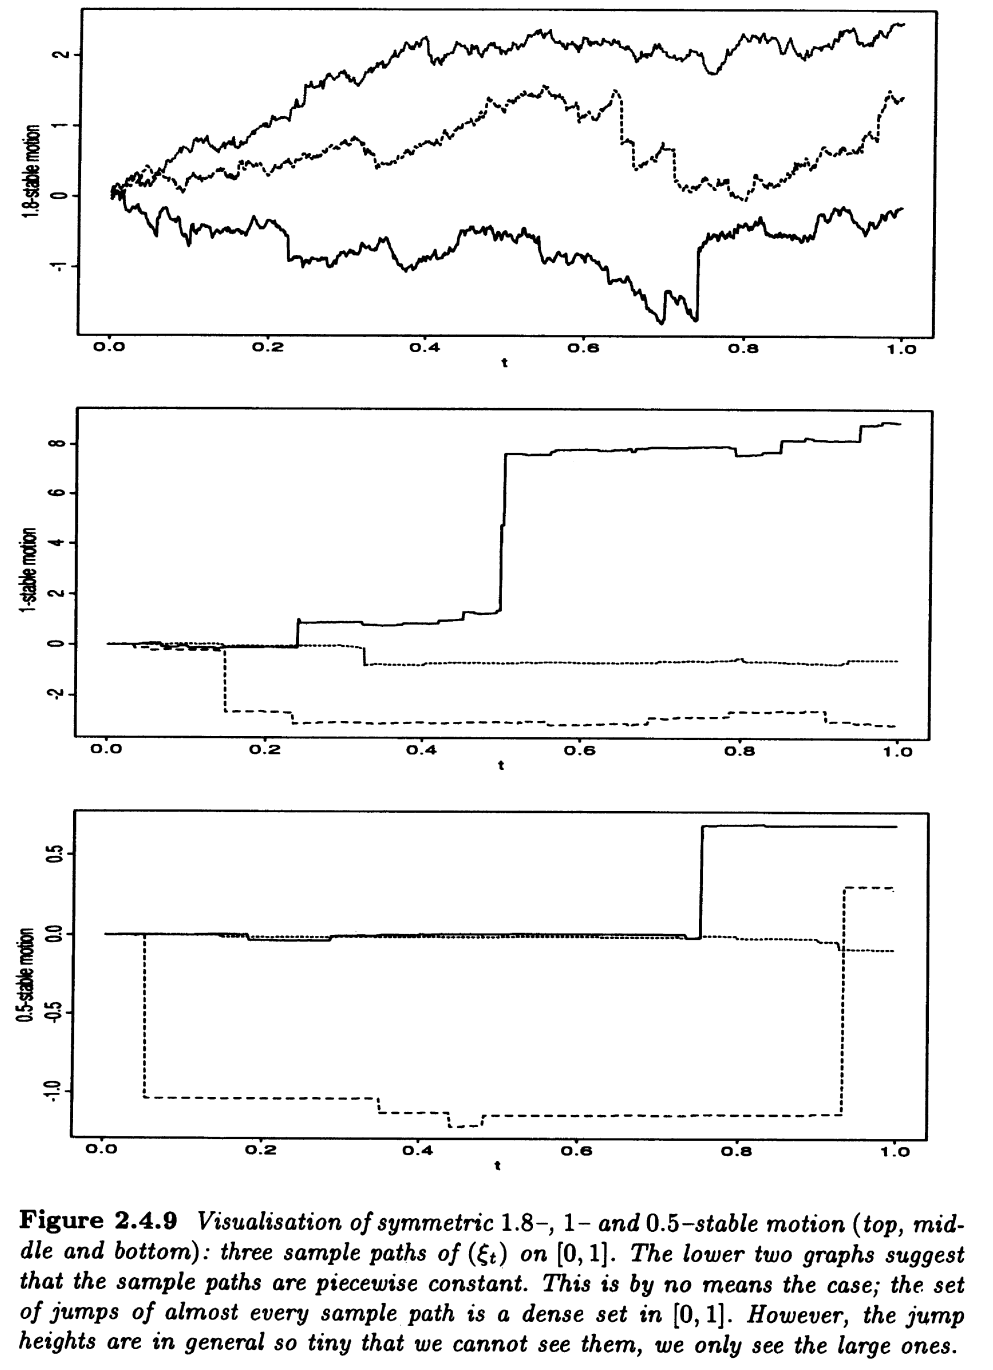
\includegraphics[height=0.50\textheight]{figures/e2-stable-process-path.png}
  \caption{$\alpha$-稳定过程的样本路径。图片来自 \cite{embrechts1997}, p.~94}
  \label{fig:e2:stable-process-path}
\end{figure}

关于平稳独立增量性，我们补充如下引理

\begin{lemma}[$\alpha$-稳定过程的增量分布]
\label{lem:ext-fclt:stable-increments}

设 $\xi(t)$ 是 $[0,1]$ 上的 α-稳定过程，则对 $0\le s<t\le 1$ 有
\[\xi(t) - \xi(s) \overset{\rm d}{=} (t-s)^{1/\alpha}\,\xi(1)\]
\end{lemma}

\begin{proof}

设 $\xi(t)$ 的特征函数为
\[\begin{aligned} \mathbb{E}[\exp\{i\lambda \xi(t)\}] = \exp\{-c(t) |\lambda|^\alpha (1 - i\beta \,\text{sign}(\lambda) z(\lambda,\alpha))\}\\ \end{aligned}\]
利用平稳独立增量，
\[\begin{aligned} \mathbb{E}[\exp\{i\lambda \xi(t)\}]  &= \mathbb{E}[\exp\{i\lambda \xi(s)\}]\, \mathbb{E}[\exp\{i\lambda (\xi(t) - \xi(s))\}] \\ &= \mathbb{E}[\exp\{i\lambda \xi(s)\}]\, \mathbb{E}[\exp\{i\lambda \xi(t-s)\} ]\\ &= \exp\{-(c(s) + c(t-s)) |\lambda|^\alpha (1 - i\beta \,\text{sign}(\lambda) z(\lambda,\alpha))\}, \end{aligned}\]
说明 $c(\cdot)$ 满足 $c(s)+c(t-s)=c(t)$、$c(0)=0$ 对 $0\le s<t\le 1$ 成立；这是一个经典的 \href{https://en.wikipedia.org/wiki/Cauchy\%27s_functional_equation}{Cauchy 方程} (Cauchy's functional equation)，其熟知的可测解为 $c(s) = c s$，其中 $c$ 为某个常数。由特征函数的性质可知 $c$ 必须为正。

因此
\[\mathbb{E}[\exp\{i\lambda (\xi(t) - \xi(s))\}] = \exp\{-c(t-s)|\lambda|^\alpha (1 - i\beta \,\text{sign}(\lambda) z(\lambda,\alpha))\}.\]
另一方面，$\xi(1)$ 的特征函数为 $\exp\{-c|\lambda|^\alpha (1 - i\beta \,\text{sign}(\lambda) z(\lambda,\alpha))\}$，从而
\[\mathbb{E}[\exp\{i\lambda (\xi(t) - \xi(s))\} ]= \mathbb{E}[\exp\{i\lambda (t-s)^{1/\alpha}\xi(1)\}]\]
由于特征函数唯一确定分布，故得
\[\xi(t) - \xi(s) \overset{\rm d}{=} (t-s)^{1/\alpha}\xi(1)\]
\end{proof}

由上述定理，我们可以得到 α-稳定过程的有限维分布表示：

\begin{corollary}\label{cor:ext-fclt:stable-finite-dimensional}
设 $0 = t_0 < t_1 < \dots < t_m \le 1$，则
\[(\xi(t_1), \xi(t_2), \dots, \xi(t_m)) \overset{\rm d}{=} \Bigl( t_1^{1/\alpha} Y_1,\; t_1^{1/\alpha} Y_1 + (t_2-t_1)^{1/\alpha} Y_2,\; \dots,\; \sum_{i=1}^m (t_i-t_{i-1})^{1/\alpha} Y_i \Bigr),\]
其中 $Y_1,\dots,Y_m$ 独立同分布，且 $Y_1 \overset{\rm d}{=} \xi(1)$。
\end{corollary}

\section{稳定泛函中心极限定理}

类似于 Donsker 定理，我们会问：\emph{是否每一个 α-稳定过程都可以作为某个部分和过程序列 }$S_n(\cdot)$* 的极限*？答案是肯定的，

\begin{theorem}[稳定泛函中心极限定理]
\label{thm:ext-fclt:stable-fclt}

设 $X_1, X_2, \dots$ i.i.d.，且属于某个位置参数 $\gamma=0$ 的非退化 α-稳定分布 $G_\alpha$ 的吸引域，即，存在缓变函数 $L(\cdot)$ 和中心化常数 $a_n$，使得
\[\frac{S_n - a_n}{n^{1/\alpha} L(n)} \overset{\rm d}\to Z_\alpha,\]
其中 $Z_\alpha$ 是服从 $G_\alpha$ 的随机变量。则，在 $\mathcal{D}[0,1]$ 空间中、配备 Skorokhod 度量 $d_0$ ，$[0,1]$ 上的随机过程
\[\xi^{(n)}(t) := \frac{1}{n^{1/\alpha} L(n)} \bigl( S_{[nt]} - a_{[nt]} \bigr)\]
弱收敛于一个 α-稳定过程 $\xi(t)$，且 $\xi(1) \overset{\rm d}{=} Z_\alpha$。

\end{theorem}

\begin{remark}

% \begin{itemize}
% \tightlist
% \item
  当 $\alpha=2$ 且 $\mathbb{E}[X_1^2] < \infty$ 时，$L(n)$ 可视为常数，且 $a_n = n\mathbb{E}[X_1]=n\mu$，定理退化为经典的 Donsker 定理。
% \item
%   吸引域条件等价于 $X_1$ 的分布函数 $F(x)$ 满足：存在缓变函数 $L_1(x)$，使得
%   \[
%   1-F(x) \sim c_+ x^{-\alpha} L_1(x),\qquad
%   F(-x) \sim c_- x^{-\alpha} L_1(x),qquad x\to\infty,
%   \]
%   其中 $c_+,c_-$ 非负，且 $c_+ + c_- > 0$。相关细节已经在
% \item
%   关于 $a_n$ ：对 $1< \alpha_n\le 2$ 都可以取 $a_n=n\mu$ 。当 $0<\alpha_n\le 1$ 时期望不存在，不过，例如 $X_1$ 的分布关于 0 对称时，则可取 $a_n=0$ 。
% \item
%   \emph{缓变函数 }(slow varying) $L(x)$ 指的是在无穷远处的缩放几乎不改变函数值： $\lim\limits_{x\to\infty} L(tx)/L(x)=1$ 对任意 $t>0$。常见例子：常函数、$\log x$、$\log \log x$ 等。
% \item
%   关于 GCLT 和吸引域更详细的内容请见 \hyperref[ext:stable-distributions]{扩展阅读《稳定分布》}。
% \end{itemize}
\end{remark}

对于稳定 FCLT，我们依然可以对其用连续映射定理，例如前文中关于 $f_1,f_2,f_3$ 函数的例子仍成立。

稳定 FCLT 有着更加广泛的应用：它可以用于模拟物理学中的超扩散 (superdiffusive) 行为、具有极端波动的金融数据，以及由非正态的 α-稳定噪声驱动的 SDE 的极限研究。%一个例子是随机梯度下降 (SGD) 的统计推断：

% \href{https://zhuanlan.zhihu.com/p/1988711005933549288}{当随机梯度没有有限方差时，我们还能做统计推断吗？}

\subsection{一个简单的模拟}

FCLT（Donsker 定理）和稳定 FCLT 不仅是一个理论结果，也提供了模拟 Brown 运动和 α-稳定过程的实用方法。例如：

\begin{itemize}
\tightlist
\item
  取 $n$ 足够大，生成 $X_1,\dots,X_n$ 独立同分布 $N(0,1)$，构造 $\widetilde S_n(t)$。得到的阶梯函数就是 Brown 运动的一个近似样本路径。
\item
  对于 α-稳定过程，可以生成独立同分布的 α-稳定随机变量 $Y_i$ ，然后构造 $\xi^{(n)}(t) = n^{-1/\alpha} \sum_{i=1}^{[nt]} Y_i$。当 $n$ 足够大时，其路径逼近真实 α-稳定过程。
\end{itemize}

如何生成独立同分布的 α-稳定随机变量？由于α-稳定分布（除少数特例外）没有显式的概率密度函数，如何高效生成其随机数曾是一个难题；目前最通用的方法是 \emph{\textbf{\href{https://en.wikipedia.org/wiki/Stable_distribution\#Simulation_of_stable_variates}{Chambers--Mallows--Stuck (CMS)}} } \textbf{\emph{算法}}，来自 \cite{chambers1976}。简而言之，取 $U\sim\mathcal U\left(-\tfrac\pi2,\tfrac\pi2\right)$ 服从均匀分布、 $E\sim\mathrm{Exp}(1)$ 服从指数分布，那么下式生成偏度系数 $\beta=0$ 、位置参数 $\gamma=0$ 、尺度参数 $c=1$ 的的标准 α-稳定分布
\[\frac{\sin(\alpha U)}{(\cos U)^{1/\alpha}}\left(\frac{\cos((1-\alpha)U)}{E}\right)^{(1-\alpha)/\alpha}\]
特别地 ，当 $\alpha=1$ 时，CMS 算法退化到生成标准 Cauchy 分布的 tan 变换 $\tan U\overset{\rm d}=\mathrm{Cauchy}(0,1)$ ；当 $\alpha=2$ 时，CMS 算法退化为 $2\sin U\sqrt{E}\overset{\rm d}=\mathcal N(0,2)$ ，再利用 $\mathrm{Exp}(1)\overset{\rm d}=-\ln (\mathcal U(0,1))$ 和 $\sin(\mathcal U(-\tfrac\pi2,\tfrac \pi2))\overset{\rm d}=\cos(2\pi\mathcal U(0,1))$ 可以得到
\[\mathcal N(0,1)\overset{\rm d}=\cos(2\pi U_1)\sqrt{-2\ln U_2},\quad  U_1,U_2\sim\mathcal U(0,1)\text{ i.i.d.}\]
这便是著名的 \href{https://en.wikipedia.org/wiki/Box\%E2\%80\%93Muller_transform}{Box--Muller 变换}。

我们写一个生成 α-稳定过程样本路径的 Mathematica 代码，固定 $n=1000$ ，

\begin{verbatim}
(* 固定参数 *)
α = 1.5;
n = 1000;
dt = 1/n;

SeedRandom[0];

(* 执行 CMS 算法生成 n 个样本 *)
U = RandomReal[{-π/2, π/2}, n];
Eexp = RandomReal[ExponentialDistribution[1], n];

inc = (dt^(1/α) Sin[U α] (Cos[U (1-α)]/Eexp)^((1-α)/α))/Cos[U]^(1/α);

(* 累积和得到路径 *)
path = Accumulate[inc];

(* 绘图 *)
ListPlot[path, DataRange -> {0, 1}, 
         PlotRange -> {{0, 1}, {-5, 5}}, 
         Joined -> If[α == 2, True, False], 
         ImageSize -> 500]
\end{verbatim}

上述程序的一次模拟结果如图~\ref{fig:e2:stable-process-simulation} 所示。

\begin{figure}[htbp]
  \centering
  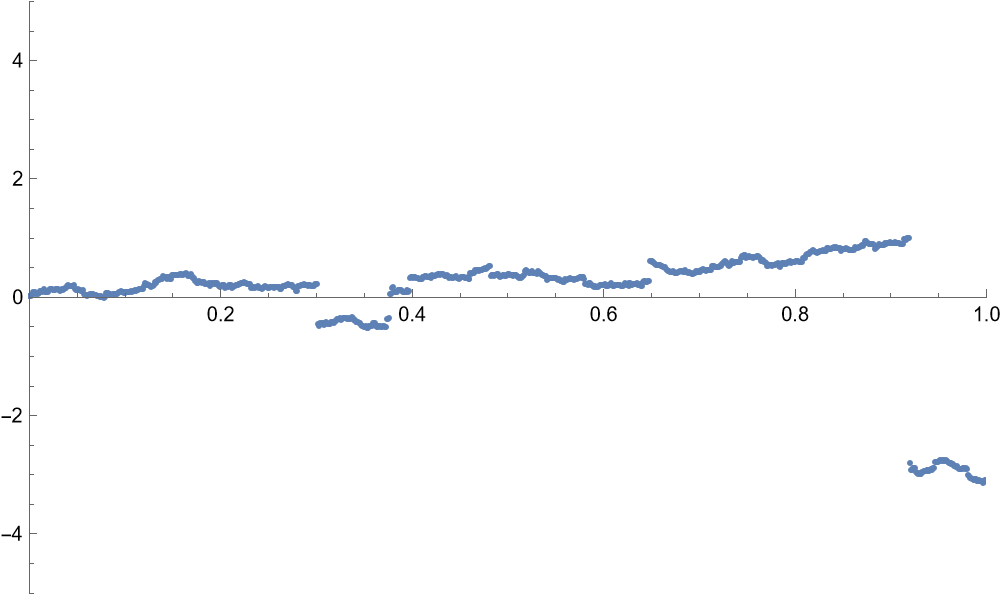
\includegraphics[width=0.88\textwidth]{figures/e2-stable-process-simulation.png}
  \caption{$\alpha$-稳定过程的模拟路径（Mathematica 13.3）}
  \label{fig:e2:stable-process-simulation}
\end{figure}

如果我们让 $\alpha$ 不断增加到 2，将看到 α-稳定过程的轨道越来越靠近连续，直至 $\alpha=2$ 时退化为 Brown 运动。可见 \href{https://demonstrations.wolfram.com/StableLevyProcess}{Wolfram Demonstrations Project}。


% \begin{figure}[htbp]
%   \centering
%   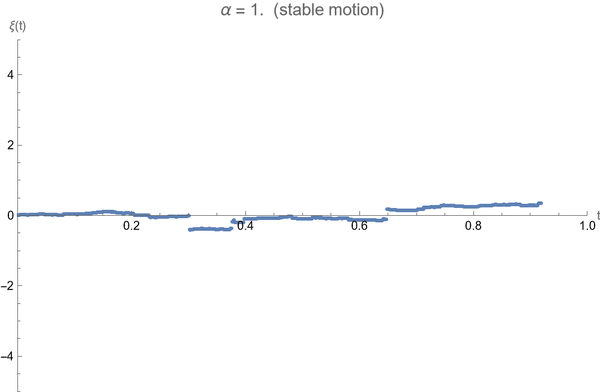
\includegraphics[width=0.88\textwidth]{figures/e2-stable-process-animation.png}
%   \caption{$\alpha$ 增加到 $2$ 时样本路径的变化；静态 PDF 展示原动画首帧（Mathematica 13.3）}
% \end{figure}

% 亦

\nocite{embrechts1997,billingsley1999}
\chapterreferences
\end{refsection}

\renewcommand{\theequation}{\thechapter.\arabic{equation}}
\renewcommand{\theHequation}{\thechapter.\arabic{equation}}
\makeatletter
\setcounter{ELEGANT@samecnt}{0}%
\renewcommand{\theELEGANT@samecnt}{\thechapter.\arabic{ELEGANT@samecnt}}%
\renewcommand{\theHELEGANT@samecnt}{\thechapter.\arabic{ELEGANT@samecnt}}%
\setcounter{exam}{0}%
\renewcommand{\theexam}{\thechapter.\arabic{exam}}%
\renewcommand{\theHexam}{\thechapter.\arabic{exam}}%
\makeatother
\renewcommand{\thesection}{\arabic{chapter}.\arabic{section}}
\renewcommand{\thesubsection}{\thesection.\arabic{subsection}}
\renewcommand{\thesubsubsection}{\thesubsection.\arabic{subsubsection}}
\makeatletter
\renewcommand{\theHsection}{\thechapter.\arabic{section}}
\renewcommand{\theHsubsection}{\thechapter.\arabic{section}.\arabic{subsection}}
\renewcommand{\theHsubsubsection}{\thechapter.\arabic{section}.\arabic{subsection}.\arabic{subsubsection}}
\makeatother

\begin{refsection}
\chapter{Delta 方法}\label{ch:delta-method}
% Generated from: Zhihu/专栏：概率与统计/渐近统计 (5)：Delta 方法_金鱼马_2026-04-23.md
在参数估计中，一个常见的情境是：对参数 $\theta\in\mathbb R^k$，我们有一列估计量 $\{T_n\}_{n=1}^\infty$，并且知道其渐近性质，如
\[
T_n\overset{P}\longrightarrow\theta,
\qquad
\sqrt n(T_n-\theta)\overset{\rm d}\longrightarrow F.
\]

但现在我们关心的不是 $\theta$ 本身，而是它的一个函数 $\phi(\theta)$，其中 $\phi:\mathbb R^k\to\mathbb R^m$。比如，$\theta$ 是正态分布的方差，我们想要估计标准差 $\sqrt\theta$；或者 $\theta$ 是两点分布的参数 $p$，我们想要估计对数几率 $\log\tfrac p{1-p}$。朴素的想法是直接用 $\phi(T_n)$ 去估计 $\phi(\theta)$，那么 $\phi(T_n)$ 的渐近分布是什么？这就是 Delta 方法回答的问题。

\section{一阶 Delta 方法}

如果 $\phi$ 是连续的，那么由连续映射定理，$T_n\overset{P}\to\theta\implies \phi(T_n) \overset{P}\to \phi(\theta)$，但这没有提供 $\phi(T_n)$ 渐近分布的信息。我们想知道的是
\[\sqrt n(\phi(T_n)-\phi(\theta))\overset{\rm d}\to \;?\]
直觉上，如果 $\phi$ 足够光滑，那么在 $\theta$ 附近， $\phi(T_n)$ 可以近似为 $\phi(\theta) + \phi'(\theta)(T_n-\theta)$。于是 $\sqrt{n}(\phi(T_n)-\phi(\theta))$ 应该近似于 $\phi'(\theta) \sqrt{n}(T_n-\theta)$，它的极限分布就是 $\phi'(\theta)F$ 。这个想法非常的简单，但非常有效。

Delta 方法本质上就是这样的一套基于 Taylor 展开的``分布传播''技术，它告诉我们在何种条件下，估计量的渐近分布和收敛速度能够被光滑变换所保持。

我们将这一想法正式地整理为定理，记 $\phi'(\theta)\in\mathbb R^{m\times k}$ 是 $\phi$ 在 $\theta$ 处的 Jacobian 矩阵，

\begin{theorem}[一阶 Delta 方法]\label{thm:ch5:first-order-delta}

设 $\phi$ 在 $\theta$ 处可微，且 $\phi'(\theta)\neq 0$；估计量 $T_n$ 满足 $a_n(T_n-\theta)\overset{\rm d}\to F$。

其中 $\{a_n\}$ 是确定的数列，有 $a_n\to \infty$。那么

\begin{enumerate}
\def\labelenumi{\arabic{enumi}.}
\tightlist
\item
  $a_n\big(\phi(T_n)-\phi(\theta)\big) - \phi'(\theta)\big(a_n(T_n-\theta)\big) \overset{P}\to 0$ ；
\item
  $a_n\big(\phi(T_n)-\phi(\theta)\big) \overset{\rm d}\to \phi'(\theta)\,F$ 。
\end{enumerate}

\end{theorem}

\begin{proof}

可微性告诉我们 $R(h):=\phi(\theta+h)-\phi(\theta)-\phi'(\theta)h=o(\|h\|)$。由 $a_n(T_n-\theta)\overset{\rm d}\to F$ 和 $a_n\to\infty$ 知 $T_n-\theta \overset{P}\to 0$，根据第~\ref{ch:random-convergence}~章的引理~\ref{lem:ch1:stochastic-plugin}，我们可将上式的 $h$ 替换为 $T_n-\theta$；再乘以 $a_n$ 即可得到
\[
\begin{aligned}
&a_n\bigl(\phi(T_n)-\phi(\theta)\bigr)
-\phi'(\theta)a_n(T_n-\theta)\\
&\qquad=o_P(a_n\|T_n-\theta\|)
=o_P(O_P(1))=o_P(1).
\end{aligned}
\]
这就证明了 (1.)。(2.) 直接由 Slutsky 定理（推论~\ref{cor:ch1:slutsky}）即得：\\\[a_n\big(\phi(T_n)-\phi(\theta)\big) = \phi'(\theta)\big(a_n(T_n-\theta)\big) + o_P(1) \overset{\rm d}\to \phi'(\theta)F\]
\end{proof}

最简单的例子是 $F$ 为正态分布的情形：

\begin{corollary}\label{cor:ch5:delta-normal}
设 $\theta\in \mathbb R^k$ 的估计量 $T_n$ 满足渐近正态性 $\sqrt n(T_n-\theta)\overset{\rm d}\to \mathcal N(0,\Sigma)$，其中 $n\to\infty$，

其中 $\Sigma\succeq 0$ 是 $k\times k$ 方阵。那么对可微函数 $\phi:\mathbb R^k\to\mathbb R^m$ ， $\phi'(\theta)\ne 0$ ，有
\[\sqrt n\big(\phi(T_n)-\phi(\theta)\big)\overset{\rm d}\to \mathcal N\big(0,\phi'(\theta)\Sigma\phi'(\theta)^\top \big)\]\end{corollary}

\section{二阶 Delta 方法}

一阶 Delta 方法很大程度上依赖于 $\phi'(\theta)\ne 0$ ；如果这一条件不满足，我们需要利用更高阶的 Taylor 展开。设 $\phi'(\theta)=0$ 但 Hessian $\phi''(\theta)\ne 0$ ，那么
\[\phi(T_n)=\phi(\theta)+\frac12\phi''(\theta)(T_n-\theta)^2+\cdots\]
那么应有
\[n\big(\phi(T_n)-\phi(\theta)\big)=\frac12\phi''(\theta)\big(\sqrt n(T_n-\theta)\big)^2\overset{\rm d}\to \frac12\phi''(\theta)F^2\]
一个很常见的情形是 $\sqrt n\bar X_n\overset{\rm d}\to \mathcal N(0,1)$ ，那么对于这样的 $\phi$ ， $n\phi(\bar{X}_n)\overset{\rm d}\to \frac12\phi''(\theta)\chi_1^2$ 。可以看到，在一阶方法中，我们乘以的系数是 $\sqrt n$ ；而在二阶方法中，由于一阶导数消失，主导项变成了二次项，我们需要乘以 $n$ 才能得到非退化的分布，这也意味着，当 $\phi'(\theta)=0$ 时， $\phi(T_n)$ 收敛到 $\phi(\theta)$ 的速度要更快。

\begin{example}[余弦变换的二阶 Delta 方法]
设 i.i.d. 随机变量 $X_1,\dots,X_n$ 有均值 0 和方差 $\sigma^2$ ，则中心极限定理告诉我们 $\sqrt{n}\bar{X}_n \overset{\rm d}\to \mathcal{N}(0,\sigma^2)$。考虑 $\phi(x)=\cos x$，在 $\theta=0$ 处 $\phi'(0)=-\sin 0 =0$，$\phi''(0)=-\cos 0 = -1$。于是
\[
-2n(\cos\bar{X}_n - 1) \overset{\rm d}\to \big(\mathcal{N}(0,\sigma^2)\big)^2 = \sigma^2 \chi_1^2.
\]

\end{example}

\begin{example}[Bernoulli 分布的 Kullback--Leibler 散度]\label{ex:ch5:bernoulli-kl}
分布 $P_\theta$ 到 $P_\eta$ 的 Kullback--Leibler（KL）散度定义为
\[
D_{\mathrm{KL}}(P_\theta\Vert P_\eta)
:=\mathbb E_\theta\left[\log\frac{p_\theta(X)}{p_\eta(X)}\right],
\qquad X\sim P_\theta,
\]
其中 $p_\theta$ 与 $p_\eta$ 分别是 $P_\theta$ 与 $P_\eta$ 的密度函数。
设 $X_1,\ldots,X_n$ i.i.d. 服从参数为 $\theta\in(0,1)$ 的 Bernoulli 分布，
$\widehat\theta_n=\bar X_n$。那么，
\[
nD_{\mathrm{KL}}(P_\theta\Vert P_{\widehat\theta_n})
\overset{\rm d}\longrightarrow \frac12\chi_1^2.
\]
\begin{proof}
Bernoulli 分布的概率质量函数为
$p_\theta(x)=\theta^x(1-\theta)^{1-x}$，其中 $x\in\{0,1\}$，因而
\[
\begin{aligned}
D_{\mathrm{KL}}(P_\theta\Vert P_{\widehat\theta_n})
&=\mathbb E_\theta\left[
  \log\frac{p_\theta(X)}{p_{\widehat\theta_n}(X)}
\right]\\
&=\theta\log\frac\theta{\widehat\theta_n}
 +(1-\theta)\log\frac{1-\theta}{1-\widehat\theta_n}.
\end{aligned}
\]
对 $t\in(0,1)$ 定义
\[
f(t):=\theta\log\frac\theta t
+(1-\theta)\log\frac{1-\theta}{1-t}.
\]
其前两阶导数为
\[
f'(t)=-\frac\theta t+\frac{1-\theta}{1-t},
\qquad
f''(t)=\frac\theta{t^2}+\frac{1-\theta}{(1-t)^2}.
\]
所以 $f(\theta)=f'(\theta)=0$，且
$f''(\theta)=1/[\theta(1-\theta)]$。由二阶 Delta 方法，
\[
\begin{aligned}
n\bigl(f(\widehat\theta_n)-f(\theta)\bigr)
&=\frac12f''(\theta)
  \bigl(\sqrt n(\widehat\theta_n-\theta)\bigr)^2+o_P(1)\\
&=\frac12\left(
  \frac{\sqrt n(\widehat\theta_n-\theta)}
       {\sqrt{\theta(1-\theta)}}
\right)^2+o_P(1)\\
&\overset{\rm d}\longrightarrow \frac12\chi_1^2,
\end{aligned}
\]
其中最后一步使用了 Bernoulli 样本均值的中心极限定理。
% 证明嵌在例子内，结尾仅保留 example 环境的一个方块。
\let\endproof\par
\end{proof}
\end{example}


当然，我们还可以向更高次项展开，单变量和多变量 $\phi$ 的情况分别如下：

\begin{theorem}[高阶 Delta 方法（一维）]\label{thm:ch5:higher-order-delta-univariate}

设 $\phi:\mathbb R\to \mathbb R$ 是单变量函数，在 $\theta\in\mathbb R$ 处 $r$ 次可微，且导数满足
\[
\phi^{(j)}(\theta)=0,\; j=1,\dots,r-1,\quad \phi^{(r)}(\theta)\neq 0.
\]

若估计量 $T_n$ 满足 $a_n(T_n-\theta)\overset{\rm d}\to F$，则
\[
\frac{a_n^{r}\big(\phi(T_n)-\phi(\theta)\big)}{\frac{1}{r!}\phi^{(r)}(\theta)} \overset{\rm d}\to F^r,\quad \text{ 当 }n\to\infty.
\]

\end{theorem}

\begin{theorem}[高阶 Delta 方法（多维）]\label{thm:ch5:higher-order-delta-multivariate}

设 $\phi:\mathbb R^k\to\mathbb R$ ，在 $\theta\in\mathbb R^k$ 处 $r$ 次可微，且所有 $1$ 阶到 $r-1$ 阶的偏导数在 $\theta$ 处均为零：
\[\frac{\partial^j\phi  (\theta)}{\partial x_{i_1}\cdots \partial x_{i_j}}=0,\quad 1\le j\le r-1,\forall i_1,\ldots,i_j\in\{1,\ldots,k\}\]
但 $r$ 阶偏导数不全为零，即存在某个 $(i_1,\dots,i_r)$ 使得
\[
\frac{\partial^r \phi (\theta)}{\partial x_{i_1}\cdots\partial x_{i_r}} \neq 0.
\]

若估计量 $T_n$ 满足 $a_n(T_n-\theta)\overset{\rm d}\to F=(F_1,\dots,F_k)$ ，则
\[a_n^{r}\,\big(\phi(T_n) - \phi(\theta)\big) \overset{\rm d}\to \frac{1}{r!}\sum_{i_1=1}^k \cdots \sum_{i_r=1}^k \left( \frac{\partial^r \phi (\theta)}{\partial x_{i_1}\cdots\partial x_{i_r}} \cdot \prod_{j=1}^r F_{i_j}\right),\quad \text{ 当 }n\to\infty.\]\end{theorem}

例如，可参考 \cite{serfling1980}, \S3.3, Theorem B。

这些结论都很复杂，在实际统计应用中很少出现。

\section{Delta 方法的例子}

下面我们通过几个经典统计例子，展示 Delta 方法的实际使用。

\subsection{样本方差的渐近正态性}

第一个例子，我们考察样本方差 $S_n:=\frac1n\sum_{i=1}^n(X_i-\bar{X})^2$ 的渐近分布。

\begin{example}[样本标准差的渐近分布]\label{ex:ch5:sd-variance}
设 $X_1,\dots,X_n$ i.i.d. 取值总体 $X$ 。记

\begin{itemize}
\tightlist
\item
  总体 $r$ 阶原点矩为 $\alpha_r:=\mathbb{E}[X^r]$ ，特别地，总体均值为 $\alpha_1$ ；
\item
  样本 $r$ 阶原点矩为 $a_{r,n}:=\frac1n\sum_{i=1}^nX_i^r$ ，特别地，样本均值为 $\bar{X}_n=a_{1,n}$ ；
\item
  总体 $r$ 阶中心矩为 $\mu_r:=\mathbb{E}[(X-\alpha_1)^r]$ ，特别地，总体方差为 $\mu_2$ 。
\end{itemize}

设总体的四阶矩存在。根据多维的中心极限定理，我们知道
\[ \sqrt{n}\begin{pmatrix} a_{1,n}-\alpha_1 \\ a_{2,n}-\alpha_2 \end{pmatrix} \overset{\rm d}\to \mathcal{N}\left(0, \mathrm{Var}\left[\begin{pmatrix} X \\ X^2 \end{pmatrix}\right]\right),\quad \text{ 当 }n\to\infty \]

另一方面，样本方差可写作 
\[ S_n := \frac1n\sum_{i=1}^n (X_i-\bar{X}_n)^2 = a_{2,n} - a_{1,n}^2 \]
考虑函数 $\phi(x_1,x_2)=x_2-x_1^2$ ，Jacobi 矩阵为 $\phi'(\alpha_1,\alpha_2) = (-2\alpha_1,\, 1)^\top\ne 0$，因此由 Delta 方法， $\sqrt{n}(S_n - \mu_2)$ 依分布收敛于正态分布 $\mathcal N(0,\Sigma)$ ，其中，
\[\begin{aligned} \Sigma&=(-2\alpha_1,1)\mathrm{Var}\left[\begin{pmatrix}X_1\\ X_1^2\end{pmatrix}\right]\begin{pmatrix}-2\alpha_1\\ 1\end{pmatrix}\\ &=\mathrm{Var}[-2\alpha_1X_1+X_1^2]\\ &=\mathrm{Var}[(X_1-\alpha_1)^2]\\ &=\mu_4-\mu_2^2 \end{aligned}\]
即，
\[\sqrt n(S_n-\mu_2)\overset{\rm d}\to \mathcal N(0,\mu_4-\mu_2^2),\quad \text{ 当 }n\to\infty\]

当然，我们知道 $S_n$ 是 $\mu_2$ 的有偏估计量，而 $s_n:=\frac n{n-1}S_n=\frac1{n-1}\sum_{i=1}^n(X_i-\bar{X})^2$ 才是无偏估计。注意到$\frac{n}{n-1}=1+\frac{1}{n-1}$，则
\[\sqrt{n}(s_{n}-\mu_2) = \sqrt{n}(S_n-\mu_2) + \underbrace{\frac{\sqrt{n}}{n-1}S_n}_{o_P(1)}\]
因此 $s_n$ 和 $S_n$ 有相同的渐近分布。

此外，如果我们考虑样本标准差 $\sqrt {S_n}$ ，则可直接对 $\phi(x)=\sqrt x$ 用 Delta 方法，由 $\phi'(\mu_2)=\frac1{2\sqrt{\mu_2}}$ 有
\[\sqrt n(\sqrt{S_n}-\sqrt{\mu_2})\overset{\rm d}\to \mathcal N\left(0,\frac{\mu_4-\mu_2^2}{4\mu_2}\right),\quad \text{ 当 }n\to\infty\]\end{example}

\subsection{渐近正态的变换}

\begin{example} \label{ex:ch5:asymptotic-normal}
设 $X_n$ 满足 $\frac{X_n-\mu}{\sigma_n^2}\overset{\rm d}\to \mathcal N(0,1)$ ，其中 $\sigma_n\to 0$ ，我们常简记为 $X_n \sim AN(\mu,\sigma_n^2)$。利用一阶 Delta 方法，有以下变换成立：

\begin{itemize}
\tightlist
\item
  $X^2_n \sim AN(\mu^2,4\mu^2\sigma_n^2)$ ，其中 $\mu\ne 0$ 。
\item
  $X_n^{-1}\sim AN(\mu^{-1},\mu^{-4}\sigma_n^2)$ ，其中 $\mu\ne 0$ 。
\item
  $e^{X_n}\sim AN(e^\mu,e^{2\mu}\sigma_n^2)$ 。
\item
  $\log |X_n|\sim AN(\log |\mu|,\mu^{-2}\sigma_n^2 )$ ，其中 $\mu\ne 0$ 。
\end{itemize}
\end{example}


值得注意的是，在例~\ref{ex:ch5:asymptotic-normal} 的第一条里，若 $\mu=0$ ，那么结论相应地要改成 $X_n^2/\sigma_n^2 \to \chi_1^2$ 。这可以推广到高维，见下例，


\begin{example}[二次型的 Delta 方法]
设 $k$ 维随机向量 $X_1,\dots,X_n$ i.i.d. ，总体有均值 $\mu$ 和协方差矩阵 $\Sigma$ ；多维中心极限定理告诉我们 \[ \sqrt{n}(\bar{X}-\mu)\overset{\rm d}\to \mathcal N_k(0,\Sigma) \]下面考察 $\phi(\bar{X})=\bar{X}^\top \bar X$ ，若 $\mu\ne 0$ ，那么 $\phi'(\mu)=2\mu$ ，故
\[\sqrt n\Big(\bar{X}^\top\bar{X}-\mu^\top\mu\Big)\overset{\rm d}\to \mathcal N(0,(2\mu)^\top\Sigma(2\mu))=\mathcal N(0,4\mu^\top\Sigma\mu)\]
当 $\mu=0$ 时又如何呢？，因为 $\sqrt{n}\bar{X} \overset{\rm d}\to \mathcal{N}_k(0,\Sigma)$，所以
\[n\bar{X}^\top\bar{X} \overset{\rm d}\to Z^\top \Sigma Z,\]
其中 $Z\sim\mathcal{N}(0,\mathbf I_k)$。这是一个加权 χ² 分布：若 $\Sigma = U^\top \operatorname{diag}(\lambda_1,\dots,\lambda_p)U$，则
\[
Z^\top\Sigma Z \overset{\rm d}= \sum_{i=1}^k \lambda_i \chi_{1i}^2.
\]

这里 $\chi_{1i}^2$ 独立同分布于 $\chi_1^2$。

由此，还可以看到收敛速度

\begin{itemize}
\tightlist
\item
  当 $\mu\ne 0$ 时， $\bar{X}^\top\bar{X}-\mu^\top\mu=O_P(1/\sqrt n)$ ；
\item
  当 $\mu=0$ 时， $\bar{X}^\top\bar{X}=O_P(1/n)$ 。
\end{itemize}
\end{example}

\subsection{方差的 χ² 检验}

\begin{example}[方差的 χ² 检验]
设 $X_1,\dots,X_n$ i.i.d. 同分布于 $\mathcal{N}(\mu,\sigma^2)$ ，其中 $\mu\in\mathbb R$ 、 $0<\sigma^2<\infty$ 未知。有如下检验问题
\[H_0:\sigma^2\le 1 \quad \iff\quad H_1:\sigma^2>1\]
在正态总体下，$\frac{nS_n}{\sigma^2}\sim\chi_{n-1}^2$。因此，可以，我们可以用如下检验统计量
\[\sum_{i=1}^n(X_i-\bar{X})^2=nS_n\]
记 $\chi^2_{n-1}(\alpha)$ 为 $\chi^2_{n-1}$ 的 $\alpha$ 分位数，那么以 $\{nS_n\le \chi^2_{n-1}(1-\alpha)\}$ 作为接受域，该检验的功效满足
\[\begin{aligned} P(nS_n>\chi^2_{n-1}(1-\alpha)\mid \sigma^2\le 1)&=P\left(\frac{nS_n}{\sigma^2}>\frac{\chi^2_{n-1}(1-\alpha)}{\sigma^2}\Big|\,\sigma^2\le 1\right)\\ &\le P(\chi^2_{n-1}>\chi^2_{n-1}(1-\alpha))\\ &=\alpha \end{aligned}\]
于是该检验有水平 $\alpha$ ，这便是我们熟知的 χ² 检验。

然而，χ² 检验对正态性十分敏感。若总体是某个非正态分布 $F$ ，应该怎么办？

\end{example}

\begin{example} 
设 $F$ 有均值 $\mu$ 和方差 $\sigma^2$ ，四阶矩存在，记 $\kappa := \frac{\mathbb{E}[(X-\mu)^4]}{\sigma^4}-3$ 为峰度，并设 $\kappa>0$ 。

一方面，用前文例~\ref{ex:ch5:sd-variance} 的结论， \[ \sqrt n\left(\frac {S_n}{\sigma^2}-1\right)\overset{\rm d}\to \mathcal N(0,\kappa+2) \]另一方面，我们知道，对于 $Z_1,\dots,Z_{n-1}\sim \mathcal N(0,1)$ i.i.d. 有 $\sum_{i=1}^{n-1}Z_i^2\sim\chi_{n-1}^2$ ，从而中心极限定理告诉我们\[ \frac{\chi_{n-1}^2-(n-1)}{\sqrt{2(n-1)}}\overset{\rm d}\to \mathcal N(0,1),\quad \text{ 当 }n\to\infty \]若以 $\xi_{1-\alpha}$ 记标准正态分布的上 $\alpha$ 分位数，则
\[\begin{aligned} & P\left(\frac{\chi_{n-1}^2-(n-1)}{\sqrt{2(n-1)}}\ge \xi_{1-\alpha}\right)\to P(\mathcal N(0,1)\ge \xi_{1-\alpha})= \alpha = P(\chi_{n-1}^2\ge \chi^2_{n-1}(1-\alpha))\\ \implies &\chi_{n-1}^2(\alpha)\approx (n-1)+\sqrt{2(n-1)}\xi_{1-\alpha}  \end{aligned}\]
从而，如果仍然直接采用 χ² 检验，我们将得到功效
\[\begin{aligned} P\Big(nS_n>\chi_{n-1}^2(1-\alpha)\Big|\,\sigma^2\le 1 \Big)&=P\left(\sqrt n\left(\frac{S_n}{\sigma^2}-1\right)>\frac{\chi^2_{n-1}(1-\alpha)-n}{\sqrt n}\,\Bigg|\,\sigma^2\le 1\right)\\ &\approx P\left(\sqrt n\left(\frac{S_n}{\sigma^2}-1\right)>\frac{(n-1)+\sqrt{2(n-1)}\xi_{1-\alpha}-n}{\sqrt n}\,\Bigg|\,\sigma^2\le 1\right)\\ &\to P\Big(\mathcal N(0,\kappa+2)>\sqrt 2\xi_{1-\alpha}\Big)\\ &=1-\Phi\left(\frac{\sqrt 2\xi_{1-\alpha}}{\sqrt{\kappa+2}}\right)\\ &>1-\Phi(\xi_{1-\alpha})=\alpha\\ \end{aligned}\]
因此 χ² 检验不再有水平 $\alpha$ 。

当然，在大样本下，χ² 检验仍然是有用的，因为我们同时可以看出当备择假设 $H_1$ 成立（ $\sigma^2>1$ ）时，
\[\begin{aligned} P( nS_n > \chi^2_{n-1}(1-\alpha)\mid \sigma^2 > 1 ) &= P  \left( \sqrt{n} \left( \frac{S_n}{\sigma^2} - 1 \right) > \frac{\sigma^{-2} \chi^2_{n-1}(1-\alpha)-n}{\sqrt{n}}\bigg| \sigma^2 > 1 \right)\\  &\approx P\left(\mathcal{N}(0, \kappa + 2) > \frac{\sigma^{-2}\big((n-1) + \xi_{1-\alpha} \sqrt{2(n-1)}\big) - n}{\sqrt{n}}\right)\\  &= 1 - \Phi\left(\frac{(\sigma^{-2} - 1)\sqrt{n}}{\sqrt{\kappa + 2}} - \frac{\sigma^{-2}}{\sqrt{n(\kappa + 2)}} + \frac{\sqrt{2}\,\xi_{1-\alpha}}{\sqrt{\kappa + 2}}\sqrt{\frac{n-1}{n}}\right)\\  &\approx 1 - \Phi\left(\frac{(\sigma^{-2} - 1)\sqrt{n}}{\sqrt{\kappa + 2}} + \frac{\sqrt{2}}{\sqrt{\kappa + 2}}\xi_{1-\alpha}\right) \\ &\to 1 \end{aligned}\]
因此 χ² 检验是相合的，即，当备择假设成立时，随着样本量增大，检验几乎一定能拒绝原假设。
\end{example}

\subsection{多项分布拟合优度检验}
 
\begin{example}[Pearson $\chi^2$ 统计量]
设有多项分布 $(n_1,\dots,n_K) \sim \text{Multinomial}(n;\,p_1,\dots,p_K)$，$p_i>0$。设经过 $n$ 次 i.i.d. 抽样后，有实际频数为 $n_i$ 、频率 $\widehat{p}_i := n_i/n$，则由多元中心极限定理，
\[X_n := \sqrt{n}\bigl(\widehat{p}_1-p_1,\dots,\widehat{p}_K-p_K\bigr)^\top \overset{\rm d}\to \mathcal{N}_K(0,\Sigma)\]
其中 $\Sigma = (\sigma_{ij})_{k\times k}$ 是协方差矩阵：
\[\begin{aligned} \sigma_{ij}&=\begin{cases} p_i(1-p_i),&\text  {若 }i=j\\ -p_ip_j,&\text{ 若 }i\ne j \end{cases}\\ &=p_i(\delta_{ij}-p_j) \end{aligned}\]
Pearson χ² 拟合优度检验采用如下检验统计量：
\[
T_n := \sum_{i=1}^K \frac{(n_i-np_i)^2}{np_i} = n\sum_{i=1}^K \frac{1}{p_i}(\widehat{p}_i-p_i)^2 = X_n^\top C X_n.
\]

其中 $C := \operatorname{diag}(p_1^{-1},\dots,p_K^{-1})$ 。根据连续映射定理，该统计量有极限
\[T_n \overset{\rm d}\to Z^\top \Sigma^{1/2} C \Sigma^{1/2} Z\]
其中 $Z\sim \mathcal N_K(0,\mathbf I_K)$ 。注意到 $\Sigma^{1/2}C\Sigma^{1/2}$ 是秩为 $K-1$ 的幂等矩阵：

\begin{itemize}
\tightlist
\item
  $(C\Sigma)_{ij} = \sum_{l} C_{il} \sigma_{lj} = p_i^{-1} \sigma_{ij} = p_i^{-1} \cdot p_i(\delta_{ij}-p_j) = \delta_{ij} - p_j$ ，于是 $(C\Sigma)^2_{ij} = \sum_l (\delta_{il}-p_l)(\delta_{lj}-p_j)=\delta_{ij}-p_j=(C\Sigma)_{ij}$ ，说明 $C\Sigma$ 幂等。
\item
  从而，与之相似的 $\Sigma^{1/2}C\Sigma^{1/2} = \Sigma^{1/2} (C\Sigma) \Sigma^{-1/2}$ 也是幂等矩阵。
\item
  其秩为 $\mathrm{tr}(A) = \mathrm{tr}(C\Sigma)=\sum_i (C\Sigma)_{ii} = \sum_i (\delta_{ii} - p_i) = \sum_i (1 - p_i) = K - 1$ 。
\end{itemize}

故 $T_n \overset{\rm d}\to \chi_{K-1}^2$，这是 Pearson χ² 检验的基本理论依据。
\end{example}
注意到 Pearson 统计量不是一个对称的统计量，这里的``不对称''指的是，它不是一个``实际频率'' $\widehat p_i$ 和``理论频率'' $p_i$ 的对称函数，因而也无法视作两个分布的``度量 (metric)''。不过，我们可以利用 Delta 方法对它进行改造：对 $\phi(x)=\sqrt x$ 用定理~\ref{thm:ch5:first-order-delta} 的第 (1.) 条，得到
\[
\sqrt n\big(\sqrt{\widehat{p_i}}-\sqrt{p_i}\big)
-\frac1{2\sqrt{p_i}}\sqrt n(\widehat p_i-p_i)
\overset{P}\to 0.
\]
于是
\[
4n\big(\sqrt{\widehat p_i}-\sqrt{p_i}\big)^2
=n\frac{(\widehat p_i-p_i)^2}{p_i}+o_P(1).
\]
这说明如下的统计量与 Pearson $\chi^2$ 检验的统计量 $T_n$ 有相同的渐近分布：
\[
T^{(g)}_n
=4n\sum_{i=1}^K(\sqrt{\widehat p_i}-\sqrt{p_i})^2
=:8nH^2(\widehat p,p).
\]
这被称作 Hellinger 统计量，其中
\[
H(\widehat p,p)
:=\sqrt{\frac12\sum_{i=1}^K(\sqrt{\widehat{p}_i}-\sqrt{p_i})^2}
=\sqrt{1-\sum_{i=1}^K\sqrt{\widehat{p}_ip_i}}
\]
是 \emph{\textbf{Hellinger 距离}}。它关于 $p_i$ 和 $\widehat p_i$ 是对称的，且取值位于 0 到 1 之间；相比于 Pearson $\chi^2$ 检验，Hellinger 距离往往拥有更好的鲁棒性。

\subsection{Wald 检验}\label{ex:ch5:wald-test}
 

\begin{example}[Wald 检验]
设有 i.i.d. $k$ 维随机向量 $X_1,X_2,\dots,X_n\sim F$ ，总体有均值 $\mu$ 和协方差矩阵 $\Sigma$ 。考虑如下双边检验问题：
\[
H_0:\mu=\mu_0\quad \iff \quad H_1:\mu\ne \mu_0.
\]

假设如下条件成立：

\begin{itemize}
\tightlist
\item
  总体 $F$ 的协方差矩阵满秩： $\Sigma\succ 0$ ；
\item
  样本的协方差矩阵 $S_n:=\frac1n\sum_{i=1}^n(X_i-\bar{X})(X_i-\bar{X})^\top$ 总满秩： $S_n\succ 0$ 。
\end{itemize}

那么，根据大数律， $S_n\overset{P}\to \Sigma$ 且 $S_n^{-1}\overset P\to \Sigma^{-1}$ 。

Wald 检验提出使用如下统计量：
\[
W_n:=n(\bar X_n-\mu_0)^\top S_n^{-1}(\bar{X}_n-\mu_0).
\]

注意到当原假设 $H_0$ 成立时：
\[\begin{aligned} W_n &= \sqrt{n}(\bar{X}-\mu_0)^\top \Sigma^{-1} \sqrt{n}(\bar{X}-\mu_0)  + \sqrt{n}\underbrace{(\bar{X}-\mu_0)^\top}_{O_P(n^{-1/2})}\underbrace{ (S_n^{-1}-\Sigma^{-1}) }_{o_P(1)}\sqrt{n}\underbrace{(\bar{X}-\mu_0) }_{O_P(n^{-1/2})}\\ &= \sqrt{n}(\bar{X}-\mu_0)^\top \Sigma^{-1} \sqrt{n}(\bar{X}-\mu_0)  +  o_P(1) \end{aligned}\]
以及 $\sqrt n\Sigma^{-1/2}(\bar{X}-\mu_0)\overset{\rm d}\to\mathcal N_k(0,\mathbf I_k)$ ，可知 $W_n\overset{\rm d}\to \chi_k^2$ ，于是可将 $\{W_n\le \chi^2_k(1-\alpha)\}$ 作为接受域。
\end{example}
Delta 方法允许我们将这套方法用在非线性假设上面： 
$$H_0:g(\mu)=0\quad \iff \quad H_1:g(\mu)\ne 0$$

其中 $g:\mathbb R^k\to\mathbb R^m$ 连续可微，且 Jacobian 矩阵 $g'(\mu)$ 总有秩 $m$ 。那么，我们可以使用如下检验统计量 

$$W_n:=ng(\bar{X})^\top\bigl(g'(\bar X)S_n g'(\bar X)^\top\bigr)^{-1}g(\bar{X})$$

由 Delta 方法，在 $H_0$ 下， 

$$\sqrt ng(\bar{X})=\sqrt n(g(\bar{X})-g(\mu))\overset{\rm d}\to \mathcal N_m\bigl(0,g'(\mu)\Sigma g'(\mu)^\top\bigr)$$

同时连续映射定理告诉我们 $g'(\bar X)S_n g'(\bar X)^\top\overset{P}\to g'(\mu)\Sigma g'(\mu)^\top$ ，再由 Slutsky 定理，立即得到 $W_n\overset{\rm d}\to \chi_m^2$

这个框架的核心是将非线性约束 $g(\theta)=0$ 通过 Delta 方法线性化，它使得我们可以把 Wald 检验用在更广泛的假设检验问题上（不局限于均值参数），设有检验问题： 
$$H_0:\theta\in\Theta_0\quad \iff\quad H_1:\theta\in\Theta\setminus\Theta_0$$

其中参数空间 $\Theta$ 是 $\mathbb R^k$ 中有内点的子集， $\Theta_0\subset \Theta$ 是一个 $k-m$ 维子流形（ $m\le k$ ），使得我们可以用 $\Theta_0=\{\theta\in\Theta:g(\theta)=0\}$ 对原假设进行刻画。
 

\begin{theorem}[Wald 统计量的渐近分布]
\label{thm:ch5:wald-asymptotic-distribution}
设
\begin{itemize}
\tightlist
\item
  $g:\Theta\to\mathbb R^m$ 连续可微，在参数空间上其 Jacobian $g'(\theta)$ 总有秩 $m$ ；
\item
  $\theta$ 有一个渐近正态估计 $\widehat\theta_n$ 使得 $a_n(\widehat\theta_n-\theta)\overset{\rm d}\to \mathcal N_k(0,\Sigma)$ ；
\item
  $\Sigma\succ 0$ ，并且存在一个相合估计使得 $\widehat \Sigma_n\overset{P}\to \Sigma$ ，同时（至少当 $n$ 充分大时） $\widehat \Sigma_n\succ 0$ 。
\end{itemize}

那么 Wald 统计量 \[ W_n=a_n^2g\big(\widehat\theta_n\big)^\top \Big(g'\big(\widehat\theta_n\big)\widehat\Sigma_ng'\big(\widehat\theta_n\big)^\top\Big)^{-1}g\big(\widehat\theta_n\big) \]就有极限分布 $\chi_m^2$ 。

\end{theorem}

\begin{remark}

\begin{itemize}
\tightlist
\item
  在一定的正则条件下，极大似然估计 (MLE) 就是渐近正态的： $\sqrt n\big(\widehat\theta_n-\theta\big)\overset{\rm d}\to \mathcal N(0,I(\theta)^{-1})$ 所以往往取 $\widehat\theta_n$ 为 MLE。上式中 $I(\theta)$ 是总体分布的 Fisher 信息矩阵，用样本 Fisher 信息矩阵估计之。可见~\ref{sec:ch7:wald-test} 节。
\item
  这里的某些条件是可以放松的，如矩阵不可逆时能用广义逆取代 (\cite{andrews1987})。
\end{itemize}
\end{remark}

\section{方差稳定变换}

在已知估计量 $T_n$有渐近分布 \[ \sqrt n(T_n-\theta)\overset{\rm d}\to \mathcal N(0,\sigma^2) \]之后，我们往往就会利用它计算置信区间，或者进行假设检验。以置信区间为例，取 \[ \texttt{CI}_n=\left[T_n-\xi_{1-\alpha/2}\frac{\sigma^2}{\sqrt n},T_n+\xi_{1-\alpha/2}\frac{\sigma^2}{\sqrt n}\right] \]就近似有置信水平 $\alpha$ 。

然而这里的渐近方差 $\sigma^2=\sigma^2(\theta)$ 往往依赖于 $\theta$，这意味着我们基于 $T_n$ 的渐近分布算出的置信区间，宽度会随 $\theta$ 变化，这往往会带来麻烦。\textbf{\emph{方差稳定变换 }} (Variance Stabilizing Transformation, VST) 的思想是：找到一个变换 $\phi$，使得 $\phi(T_n)$ 的渐近方差为常数 $c^2$（与 $\theta$ 无关）。

由 Delta 方法（简单起见，这里假设 $\phi$ 是映射到 $\mathbb R$ 的连续函数， $\phi'(\theta)\ne 0$ ），
\[\sqrt{n}(\phi(T_n)-\phi(\theta)) \overset{\rm d}\to \mathcal{N}\bigl(0,\,(\phi'(\theta))^2\sigma^2(\theta)\bigr)\]
我们希望 $(\phi'(\theta))^2\sigma^2(\theta)=c^2$，即
\[\phi'(\theta) = \frac{c}{\sigma(\theta)} \quad \Longrightarrow \quad \phi(\theta) = c\int \frac{{\rm d}\theta}{\sigma(\theta)}\]
常数 $c$ 可以任意选取（通常取 $c=1$ 或 $c$ 使得变换后方差为 1）。

\begin{example}[Fisher's $z$-transformation]\label{ex:ch5:fisher-z}
设 $(X_1,Y_1),(X_2,Y_2),\dots$ i.i.d. 同分布于二维正态分布，总体相关系数为 

$$\rho = \frac{\mathrm{Cov}[X,Y]}{\sqrt{\mathrm{Var}[X]\,\mathrm{Var}[Y]}} = \frac{\mathbb{E}[(X-\mu_X)(Y-\mu_Y)]}{\sigma_X\,\sigma_Y}$$ 

样本相关系数定义为
\[
r_n:={\frac {\sum _{i=1}^n(X_i-{\bar {X}})(Y_i-{\bar {Y}})}{{\sqrt {\sum _{i=1}^n(X_i-{\bar {X}})^2}}{\sqrt {\sum _{i=1}^n(Y_i-{\bar {Y}})^2}}}}.
\]
可以证明 $r$ 是 $\rho$ 的渐近正态估计：
\[
\sqrt{n}(r_n - \rho) \overset{\rm d}\to\mathcal N(0, (1-\rho^2)^2).
\]

% 具体过程比较繁琐，从略。可见

% \href{https://www.zhihu.com/question/51402458/answer/1975264119998394908}{the delta method 是干什么的？}

则 VST 是
\[
\phi(\rho)=\int\frac1{1-\rho^2}\mathrm d\rho=\frac12\log\frac{1+\rho}{1-\rho}=\operatorname{arctanh} \rho.
\]
从而
\[
\sqrt n\Big(\operatorname{arctanh}r_n-\operatorname{arctanh} \rho\Big)\overset{\rm d}\to\mathcal N(0,1).
\]

对任意的 $\rho$ 成立。据此可以构造出近似的 $\alpha$ 置信区间 \[ \left(\tanh \left(\operatorname{arctanh} r_n-\frac{\xi_{1-\alpha/2}}{\sqrt n}\right),\tanh \left(\operatorname{arctanh} r_n+\frac{\xi_{1-\alpha/2}}{\sqrt n}\right)\right) \]这种``取样本相关系数 arctanh''的方法叫做 \href{https://en.wikipedia.org/wiki/Fisher_transformation}{Fisher z-变换}。图~\ref{fig:ch5:fisher-z-transform} 给出了一个例子：对相关系数 $\rho=0.5$ 的总体重复模拟 $10^5$ 次，每次使用 12 个独立样本计算 $r_n$，并分别绘制 Fisher 变换之前（左）和之后（右）的直方图。可以看到，除了稳定方差外，Fisher $z$-变换的另一优点是将分布对称化。

\begin{figure}[htbp]
  \centering
  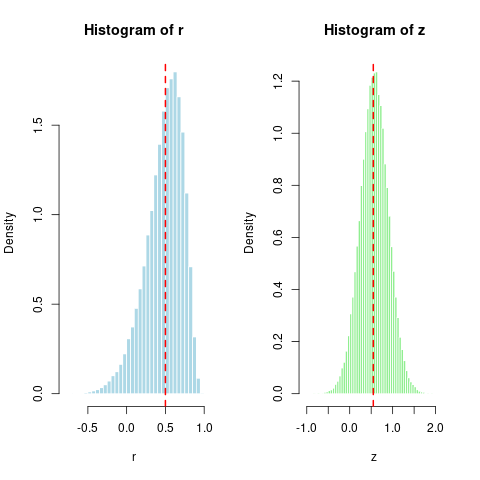
\includegraphics[width=0.62\textwidth]{figures/05-fisher-z-transform.png}
  \caption{Fisher $z$-变换前后的模拟分布（R 绘制）}
  \label{fig:ch5:fisher-z-transform}
\end{figure}

\begin{verbatim}
m = 10^5; r=numeric(m);  n = 12
 for(i in 1:m) {
    u1 = rnorm(n); u2 = rnorm(n);  u3=rnorm(n)
    x = u1 + u2;  y = u2 + u3
    r[i] = cor(x, y) }

summary(r); sd(r)
## Min. 1st Qu.  Median    Mean 3rd Qu.    Max. 
## -0.7282  0.3429  0.5176  0.4822  0.6590  0.9804 
## 0.23916

# Fisher z transformation
z <- 0.5 * log((1 + r) / (1 - r))

summary(z); sd(z)
## Min. 1st Qu.  Median    Mean 3rd Qu.    Max. 
## -0.9248  0.3573  0.5731  0.5746  0.7910  2.3083 
## 0.3310624
\end{verbatim}


\end{example}

\begin{example}[Tukey's Hanging Rootgram]
设 i.i.d. 随机变量 $X_1,X_2,\dots,X_n\sim F$ ，有密度函数 $f$ 。\textbf{\emph{核密度估计 }} (KDE) 或者称 Parzen-Rosenblatt 密度估计如下：
\[\widehat{f}_{nh}(x) = \frac{1}{nh}\sum_{i=1}^n K\!\left(\frac{x-X_i}{h}\right)\]
其中 $K$ 是核函数（满足适当正则条件），如标准正态密度； $h=h(n)$ 是平滑带宽。

有这样的结论 \cite{parzen1962}：若平滑带宽满足：当 $n\to\infty$ 时， $nh\to \infty$ 但 $nh^5\to 0$，那么KDE 有渐近正态性：
\[
\sqrt{nh}\big(\widehat f_{nh}(x)-f(x)\big)\overset{\rm d}\to \mathcal N\left(0, {\textstyle f(x)\int K^2(y){\rm d}y}\right).
\]

因此 $\widehat{f}_{nh}(x)\sim AN\left(f(x), \textstyle{\frac{\int K^2(y){\rm d}y}{nh}f(x)}\right)$ ，忽略掉常数，其渐近方差依赖于 $f(x)$ 。于是 VST 可以取
\[
\phi(f) =\frac12 \int \frac{{\rm d}f}{\sqrt{f}} = f^{1/2}.
\]
从而，对 $\big(\widehat{f}_{nh}(x)\big)^{1/2}$ ，有
\[
\big(\widehat{f}_{nh}(x)\big)^{1/2}\sim AN\left(f(x), \frac{\int K^2(y){\rm d}y}{4nh}\right).
\]

\end{example}

关于密度估计，有一本经典的参考教材 \cite{silverman1986}，介绍得十分详尽。

% 最后要说的是，在现代统计学中，由于 Bootstrap（自助法）的普及，我们往往可以直接通过重采样来计算复杂置信区间。但除了构建置信区间，VST 还有两个重要作用：一是满足经典模型（如方差分析、线性回归）的同方差性假设；二是去除估计量方差与均值的耦合关系，使得我们可以更客观地比较不同总体的离散程度。

\nocite{vandervaart1998}
\chapterreferences
\end{refsection}

\begin{refsection}
\chapter{矩估计}\label{ch:method-of-moments}
% Generated from: Zhihu/专栏：概率与统计/渐近统计 (6)：矩估计_金鱼马_2026-04-28.md
\section{矩估计}

\subsection{基本概念}

``矩 (moment)'' 是一个来自于物理学的概念：一阶矩代表质心，二阶代表转动惯量。统计学中借用了这一概念年，用其指代随机变量幂次的期望。

% \href{https://www.zhihu.com/question/19915565}{统计学中「矩」这个概念是怎么引入的？它为什么被称为矩？它与物理意义上的矩有什么相同与不同？}

对 $\mathbb R$ 上的参数族 $P_\theta$ ，其中 $\theta=(\theta_1,\theta_2,\dots,\theta_k)^\top\in\mathbb R^k$ 是我们感兴趣的参数，我们记 $r$ 阶原点矩为 $\alpha_r:=\mathbb{E}_\theta[X^r]=\int x^r\mathrm{d}P_\theta(x)$ ，并设其有限； $X_1,\dots,X_n\sim P_\theta$是 i.i.d. 样本，记样本 $r$ 阶原点矩为 $a_{r,n}:=\frac1n\sum_{j=1}^nX_{j}^r$ 。

矩方法 (Method of Moments, MOM) 是一种经典的参数估计方法。简单来说，这种方法将总体矩表示为目标参数的函数，设目标参数是
\[ \begin{cases} \alpha_1&=\alpha_1(\theta_1,\theta_2,\dots,\theta_k)\\ \vdots\\ \alpha_r&=\alpha_r(\theta_1,\theta_2,\dots,\theta_k) \end{cases} \]

然后用``插入原则 (plug-in principle)''的思想，用样本矩替代总体矩，得到矩方程
\[\begin{cases} a_{1,n}&=\alpha_1\big(\widehat\theta_{1,n},\widehat\theta_{2,n},\dots,\widehat\theta_{k,n}\big)\\ \vdots\\ a_{r,n}&=\alpha_r\big(\widehat\theta_{1,n},\widehat\theta_{2,n},\dots,\widehat\theta_{k,n}\big) \end{cases}\]
求解方程得到的 $\widehat\theta_1,\dots,\widehat\theta_k$ 便是矩估计。一言以蔽之：列出矩与参数的方程，用样本矩代替总体矩，从而解出参数便是矩估计。

\begin{example}[均匀分布的矩估计]
设 $-\infty<a<b<\infty$ ， $U\sim \mathcal U([a,b])$ 是区间 $[a,b]$ 上均匀分布的随机变量，我们计算一、二阶矩\[ \begin{cases} \alpha_1&=\mathbb{E}[U]=\dfrac{a+b}{2}\\ \alpha_2&=\mathbb{E}[U^2]=\dfrac{a^2+ab+b^2}{3} \end{cases} \]

对于 i.i.d. $U_1,\dots,U_n$样本，计算出样本 1、2 阶矩 $a_{1,n}$ 、 $a_{2,n}$ ，求解矩方程即可得到
\[\begin{aligned} \widehat{a}_n&=a_{1,n}-\sqrt{3(a_{2,n}-a_{1,n}^2)}\\ \widehat{b}_n&=a_{1,n}+\sqrt{3(a_{2,n}-a_{1,n}^2)}\\  \end{aligned}\]
\end{example}


一般来说，从不同的矩出发估计某个参数，会得到不同的估计，例如，Poisson 分布 $\mathrm{Poisson}(\lambda)$ 中的参数 $\lambda$ 既是均值又是方差，按矩估计法，既可以用样本均值，也可以用样本方差来估计之，因此，矩估计法应视为一个 ad-hoc 的原则，而并没有一个一般的准则（这也是它的一个局限性）。一般来说，在经典矩估计中，应优先考虑使用阶数较低的矩。

当然，好奇的读者一定会问：为什么一定要选择``矩''？或者说，为什么一定要找`` $X$ 幂次的期望''？可不可以更自由一些呢？答案也是肯定的，我们给出如下定义

\begin{definition*}[矩估计]
设 $X_1,\ldots,X_n\sim P_\theta$ i.i.d.，$\theta_0\in\Theta$ 是真实参数，参数空间 $\Theta\subset\mathbb R^k$。选取 $k$ 个已知函数 $f_1,\ldots,f_k$，并记向量 $f:=(f_1,\ldots,f_k)^\top$。定义总体矩为

$$\alpha_f(\theta):=\mathbb{E}_\theta[f(X)] = \int f(x)\,\mathrm{d}P_\theta(x)$$

样本矩为 $a_{f,n}:=\frac1n\sum_{j=1}^nf(X_j)$

那么， 通过解方程 $\alpha_f(\widehat\theta_n)=a_{f,n}$，也就是， 

$$\mathbb{E}_{\widehat \theta_n}[f_r(X)]=\frac{1}{n}\sum_{j=1}^n f_r(X_j),\quad r=1,\dots,k$$

所得到的 $\widehat\theta$ 便是 $\theta_0$ 的\textbf{\emph{矩估计 }} (moment estimator, ME)。
\end{definition*}
这种方法是现代统计学的奠基人之一 K. Pearson 在 20 世纪初研究曲线拟合时提出的, 至今仍不失为一 种重要而常用的方法。当取 $f_r(x)=x^r$ 时，就是经典的矩估计。

\subsection{矩估计的渐近正态性}

直觉上，当样本量很大时，样本矩 $a_{f,n}$ 会以 $\sqrt{n}$ 的速度收敛到正态分布。当 $\alpha_f:\mathbb R^k\to\mathbb R^k$ 是单射时， $\widehat\theta_n=\alpha_f^{-1}(a_{f,n})$ ；如果 $\alpha_f^{-1}$ 是可微的，并且 $\mathbb{E}_{\theta_0}[f(X)f(X)^\top]<\infty$ ，那么根据 Delta 方法，矩估计 $\hat{\theta}_n$ 也应该有正态极限。关键在于保证反函数的存在性和可微性。

\begin{theorem*}[逆映射定理]：设 $A$ 是 $\mathbb R^k$ 中的开子集， $g:A\mapsto \mathbb R^k$ 在 $a\in A$ 处连续可微，并且在 $a$ 的一个邻域内可微，若 Jacobian 矩阵 $g'(a)\in\mathbb R^{k\times k}$ 是非奇异的，那么

\begin{enumerate}
\def\labelenumi{\arabic{enumi}.}
\tightlist
\item
  存在 $a$ 的一个开邻域 $U$ 和 $\mathbb R^k$ 的开子集 $V$ ，使得 $g$ 一对一（单射）地将 $U$ 映射到 $V$ ，
\item
  逆映射 $g^{-1}:V\to U$ 存在，使得 $g^{-1}(g(x))=x$ ，并且 $g^{-1}$ 连续可微。
\end{enumerate}

这个结论在很多分析学教材中都会介绍，例如可参考 \cite{munkres1997} 的 Theorem 8.3。

\end{theorem*}

利用反函数定理，我们可以严格叙述和证明矩估计的渐近正态性，


\begin{theorem}[矩估计的相合性和渐近正态性]\label{thm:ch6:mom-asymptotic-normality}

若 $\alpha_f(\theta) = \mathbb{E}_\theta [f(X)]$ 在开集 $\Theta \subset \mathbb{R}^k$ 上是单射，且在真实参数 $\theta_0\in\Theta$ 处连续可微，且 Jacobian 矩阵 $\alpha_f'(\theta_0)$ 非奇异， $\mathbb{E}_{\theta_0}[f(X)f(X)^\top] < \infty$，那么以概率 1 当 $n$ 充分大时，矩估计方程存在唯一解 $\widehat\theta_n$ ，并且
\[\sqrt n\big(\widehat\theta_n-\theta_0\big)\overset{\rm d}\to \mathcal N_k\left(\bm 0,(\alpha_f'(\theta_0))^{-1}\Sigma_f\left((\alpha_f'(\theta_0))^{-1}\right)^\top\right)\]
其中 $\Sigma_f:=\mathbb{E}_{\theta_0}[f(X)f(X)^\top]-(\mathbb{E}_{\theta_0}[f(X)])(\mathbb{E}_{\theta_0}[f(X)])^\top$ 。

\end{theorem}

\begin{proof}

由逆映射定理，存在 $\theta_0$ 的开邻域 $U$ 和 $\alpha_f(\theta_0)$ 的开邻域 $V$ ，使得 $\alpha_f$ 将 $U$ 一对一地映射到 $V$ ，因而存在逆映射 $\alpha_f^{-1}:V\to U$ 。由强大数律，在 $P_{\theta_0}$ 下，
\[
a_{f,n}=\frac1n\sum_{j=1}^nf(X_j)\overset{\text{a.s.}}\to \alpha_f(\theta_0)\in V,\quad \text{ 当 }n\to\infty.
\]

所以以概率 1 当 $n$ 充分大时， $a_{f,n}\in V$ ，这时 $\widehat\theta_n=\alpha_f^{-1}(a_{f,n})$ 存在，并且根据连续映射定理，这是一个强相合估计：
\[
\widehat\theta_n=\alpha_f^{-1}(a_{f,n})\overset{\text{a.s.}}\to \alpha_f^{-1}(\alpha_f(\theta_0))=\theta_0,\quad\text{ 当 }n\to\infty.
\]

由于 $\mathbb{E}_{\theta_0}[f(X)f(X)^\top] < \infty$ ，中心极限定理告诉我们
\[
\sqrt n\big(a_{f,n}-\alpha_f(\theta_0)\big)\overset{\rm d}\to\mathcal N(0,\Sigma_f).
\]

再对 $\alpha_f^{-1}$ 使用第~\ref{ch:delta-method}~章的 Delta 方法定理~\ref{thm:ch5:first-order-delta}，便得到结论。注意这里 $\left(\alpha_f^{-1}\right)'=\left(\alpha_f'\right)^{-1}$。

\end{proof}

\begin{remark}

\begin{itemize}
\tightlist
\item
  这个证明亦可参考 \cite{zhaolincheng2016} 一书的 定理 5.5。
\item
  ``以概率 1 当 $n$ 充分大时某某事件发生''的说法在大样本估计中经常见到，从无穷乘积空间中理解最好：记样本概率空间为 $(X,\mathscr B_X,P_{\theta_0})$ ，其无穷乘积空间为 $(X^\infty,\mathscr B^\infty,P_{\theta_0}^\infty)$ ，存在 $A\subset X^\infty$ 使得 $P_{\theta_0}^\infty(A)=1$ ，使得点 $(X_1,X_2,\dots)\in A$ 时存在 (与此点相关的) 正整数 $N$ ，当 $n>N$ 时，对 $(X_1,\dots,X_n)$ 有``某某事件发生''。在本证明中， 我们指的是：对 $n>N$ ， $(X_1,\dots,X_n)$的样本矩 $a_{f,n}\in V$ ，从而矩方程有唯一解 $\widehat\theta_n=\widehat\theta_n(X_1,\dots,X_n)$ 。这个叙述来自 \cite{chenxiru2009} 一书的 p.150。
\end{itemize}

\begin{example}[Beta 分布的矩估计]
考虑来自 Beta 分布 $\mathrm{Beta}(\alpha,\beta)$ 的 i.i.d. $X_1,\dots,X_n$，其密度为

\[
p(x;\alpha,\beta)=\frac1{\mathrm{B}(\alpha,\beta)}
x^{\alpha-1}(1-x)^{\beta-1},\qquad 0<x<1,
\]
其中 $\alpha>0,\beta>0$ 是我们感兴趣的未知参数， $\mathrm{B}(\alpha,\beta)$ 代表 Beta 函数。很容易算出总体原点矩
\[\begin{aligned}\alpha_k=\mathbb{E}[X^k]&=\frac1{\mathrm{B}(\alpha,\beta)}\int_{\mathbb R} x^{\alpha+k-1}(1-x)^{\beta-1}\mathrm{d}x\\ &=\frac{\mathrm{B}(\alpha+k,\beta)}{\mathrm{B}(\alpha,\beta)}\\ &=\frac{\Gamma(\alpha+k)}{\Gamma(\alpha)}\frac{\Gamma(\alpha+\beta)}{\Gamma(\alpha+\beta+k)}\\ &=\prod_{r=0}^{k-1}\frac{\alpha+r}{\alpha+\beta+r} \end{aligned}\]
特别地， $\mathbb{E}[X]=\frac{\alpha}{\alpha+\beta}$ 、 $\mathbb{E}[X^2]=\frac{\alpha(\alpha+1)}{(\alpha+\beta)(\alpha+\beta+1)}$ 。记样本 1、2 阶原点矩为 $a_{1,n}$ 、 $a_{2,n}$ ，构造矩估计方程，可以解出参数 $\alpha,\beta$ 的矩估计，
\[\left\{\begin{aligned} \widehat\alpha_n&=a_{1,n}\left(\frac{a_{1,n}(1-a_{1,n})}{a_{2,n}-a_{1,n}^2}-1\right)\\ \widehat\beta_n&=(1-a_{1,n})\left(\frac{a_{1,n}(1-a_{1,n})}{a_{2,n}-a_{1,n}^2}-1\right) \end{aligned} \right.\]
记 $\theta=(\alpha,\beta)^\top$ 、 $f(x)=(x,x^2)^\top$ ，那么
\[
\alpha_f(\theta)=(\mathbb{E}_\theta[X],\mathbb{E}_\theta[X^2])^\top=\left(\frac\alpha{\alpha+\beta},\frac{\alpha(\alpha+1)}{(\alpha+\beta)(\alpha+\beta+1)}\right)^\top.
\]

容易验证 $\alpha_f^{-1}\in C^\infty(\mathbb R_+^2)$ ，则根据定理~\ref{thm:ch6:mom-asymptotic-normality}， $\widehat\theta_n=(\widehat\alpha_n,\widehat\beta_n)^\top=\alpha_f^{-1}(\theta)$ 是相合估计，满足渐近正态性。由\[\alpha'_f(\theta)=\begin{pmatrix} \dfrac{\beta}{(\alpha+\beta)^2} & -\dfrac{\alpha}{(\alpha+\beta)^2} \\ -\dfrac{\beta(\alpha+1)(\alpha+\beta+1) + \alpha\beta (\alpha+\beta)}{(\alpha+\beta)^2(\alpha+\beta+1)^2} & -\dfrac{\alpha(\alpha+1)(2(\alpha+\beta)+1)}{(\alpha+\beta)^2(\alpha+\beta+1)^2} \end{pmatrix}\]和\[\Sigma_f = \begin{pmatrix} \mathrm{Var}[X] & \mathrm{Cov}[X, X^2] \\ \mathrm{Cov}[X, X^2] & \mathrm{Var}[X^2] \end{pmatrix}= \begin{pmatrix} \alpha_2 - \alpha_1^2 & \alpha_3 - \alpha_1\alpha_2 \\ \alpha_3 - \alpha_1\alpha_2 & \alpha_4 - \alpha_2^2 \end{pmatrix}\]
可以算出渐近协方差（过于繁琐，不再显式展开）。


\end{example}

\subsection{与极大似然估计的联系}

在某些特殊情况下，极大似然估计居然也可以视作是特殊的矩估计！这里的``特殊情况''是，总体分布族要属于\textbf{\emph{\href{https://en.wikipedia.org/wiki/Exponential_family}{指数型分布族}}} (Exponential family)。简单来说，指数型分布族是一大类密度函数形如
\[
p(x;\theta)=c(\theta)h(x)\exp\{\theta^\top T(x)\}
\]
的分布族，其中 $c(\theta),h(x),T(x)$ 是给定的函数。这涵盖了很多的常见分布（如正态、Gamma、Beta、Bernoulli、Poisson、指数、χ² 等），并且有良好的统计性质。%关于指数型分布族的更详细内容，读者可以参考

% \href{https://zhuanlan.zhihu.com/p/27452245086}{数理统计 (1) 基本概念}

% \href{https://zhuanlan.zhihu.com/p/596078459}{【高等统计学】1. 指数族}

我们主要利用它的 MLE 性质。首先有似然函数 

$$L_x(\theta)=\log p(x;\theta)=\log c(\theta)+\log h(x)+\theta^\top T(x)$$

从而得分函数 (score function) 为 \[ L'_x(\theta)=\frac{c'(\theta)}{c(\theta)}+T(x)=T(x)-\mathbb{E}_\theta[T(X)] \]这里的第二个等号是因为 $\mathbb{E}_\theta[L'_X(\theta)]=0$ 可以推出 $\frac{c'(\theta)}{c(\theta)}=-\mathbb{E}_\theta[T(X)]$ 。极大似然估计是求解对数似然方程 \[ \frac{1}{n}\sum_{i=1}^n L'_{X_i}(\theta) = 0 \]的根作为估计；若记
\[\begin{aligned} a_{T,n}&=\frac1n\sum_{j=1}^nT(x_j)\\ \alpha_T(\theta)&=\mathbb{E}_\theta[T(x)] \end{aligned}\]
那么似然方程正好是 $\alpha_{T}(\theta)=a_{T,n}$ ！所以此时 MLE 和函数 $T$ 对应的矩估计是相同的。

指数型分布族的良好解析性质保证 $c(\theta)$ 任意阶导数存在，以及 $T(X)$ 各阶矩存在，进一步，这些矩可以通过对 $\ln c(\theta)$ 求导获得：
\[\begin{aligned} \mathbb{E}_\theta[T(X)]&=(\ln c(\theta))'=\frac{c'(\theta)}{c(\theta)}=\alpha_T(\theta)\\ \mathrm{Var}_\theta[T(X)]&=(\ln c(\theta))''=\alpha_T'(\theta) \end{aligned}\]
% （见 \href{https://zhuanlan.zhihu.com/p/27452245086}{数理统计 (1) 基本概念} 的定理 1.1。）
这里 $\mathrm{Var}_\theta[T(X)]$ 代表 $T(X)$ 的协方差矩阵，我们设其满秩。

注意到 Fisher 信息矩阵是
\[
\mathcal I_\theta=\mathrm{Var}_\theta[L'_X(\theta)]=\mathrm{Var}_\theta\big[T(x)-\mathbb{E}_\theta[T(X)]\big]=\mathrm{Var}_\theta[T(x)].
\]

我们得到了重要的关系：
\[
\mathcal I_\theta=\mathrm{Var}_\theta[T(x)]=\alpha_T'(\theta).
\]

于是根据定理~\ref{thm:ch6:mom-asymptotic-normality}， \[ \sqrt n\big(\widehat\theta_n-\theta_0\big)\overset{\rm d}\to \mathcal N\Big(0,(\alpha_T'(\theta_0))^{-1}\mathrm{Var}_\theta[T(X)]((\alpha_T'(\theta_0))^{-1})^\top\Big)=\mathcal N(0,\mathcal I^{-1}_{\theta_0}) \]说明 $\widehat\theta_n$ 是渐近有效的，或者说，它是最佳渐近正态 (BAN) 估计。

% 也可以参考 \href{https://zhuanlan.zhihu.com/p/1909962170453726655}{数理统计 (16) : 极大似然估计 - 下 - MLE 的渐近正态性} 的定理 16.2。

在参数估计中，如果密度函数是已知的，那么相比于矩估计，其实大家还是更爱用极大似然估计 (MLE)，因为矩估计往往不如 MLE 更有效。下面一个例子表明，从渐近方差的角度看，矩估计可以任意糟糕。

\begin{example}[矩估计可能无定义]
考虑 $X_1,\dots,X_n\sim\mathcal N(\theta,1)$ i.i.d.， $\theta>0$ 是未知参数。总体的二阶矩是 $\theta^2+1$ ，矩估计方程如下：
\[
\widehat\theta_n^2+1=\frac1n\sum_{j=1}^nX_j^2\enspace\implies\enspace \widehat\theta_n=\left(\frac1n\sum_{j=1}^nX_j^2-1\right)^{1/2}.
\]

由 $\mathrm{Var}[X^2]=2+4\theta^2$ 有
\[
\frac1{\sqrt n}\sum_{j=1}^n\big(X_j^2-(1+\theta^2)\big)\overset{\rm d}\to \mathcal N(0,2+4\theta^2).
\]
从而，对 $\sqrt{x}$ 用 Delta 方法，我们得到
\[
\sqrt n\big(\widehat\theta_n-\theta\big)\overset{\rm d}\to \mathcal N\left(0,\left(\frac1{2\theta}\right)^2(2+4\theta^2)\right)=\mathcal N\left(0,\frac{1}{2\theta^2}+1\right).
\]

当 $\theta\to 0^+$ 时这里的渐近方差可以任意大。
\end{example}

那么，相比于 MLE，矩估计就一无是处了吗？也不是，MLE 一般要求我们知道完整的密度函数 $p(x;\theta)$ ------在回归问题中可以是条件密度 $p(y|x;\theta)$ ，在面板数据模型 (panel data) 中可以是 $p(y_t|x_t;\theta)$ ------但总之需要知道密度。这实际上对数据的生成作出了很强的限制。而矩估计只需要我们知道总体矩 $\alpha_r$ 的形式，这个限制是更宽松的。

最简单的例子是最小二乘法，对线性模型 $y_i=\beta^\top x_i+\varepsilon_i$ ，MLE 的做法需要假设 $\varepsilon_i$ 独立同分布于正态总体： $\varepsilon_i \sim \mathcal{N}(0,\sigma^2)$；矩估计则可以不假设任何分布性质，只需要一个矩条件 $\mathbb{E}[x_i\epsilon_i]=\mathbb{E}[x_i(y_i-x_i^\top\beta)]=0$ 成立，此时的矩估计正是最小二乘估计。%可见：

% \href{https://www.zhihu.com/question/55084299/answer/1685871552}{最小二乘法只有在因变量服从正态分布时才能用吗？}

下面是一个稍微复杂点的 

\begin{example}[Yule--Walker 估计]
考虑一个零均值、平稳的 $\mathrm{AR}(p)$ 过程 $\{X_t\}_{t\in\mathbb Z}$ ：
\[X_t = \phi_1 X_{t-1} + \phi_2 X_{t-2} + \dots + \phi_p X_{t-p} + \varepsilon_t\]
其中 $\varepsilon_t\sim WN(0,\sigma^2)$ 是白噪声序列，独立于所有过去值 $X_{t-k}$ 。我们想要估计自回归系数 $\phi_1, \dots, \phi_p$ 和白噪声方差 $\sigma^2$ 。对模型两边同乘 $X_{t-k}$ （$k=1,\dots,p$）并取期望，利用 $\mathbb{E}[\varepsilon_t X_{t-k}] = 0$，立即可得 \textbf{\emph{Yule--Walker 方程}} ：
\[ \gamma_k = \phi_1 \gamma_{k-1} + \phi_2 \gamma_{k-2} + \dots + \phi_p \gamma_{k-p}, \quad k=1,\dots,p \]其中 $\gamma_k:=\mathbb{E}[X_iX_{i-k}]$ 。上述方程写成矩阵形式为
\[\begin{pmatrix} \gamma_1 \\ \gamma_2 \\ \vdots \\ \gamma_p \end{pmatrix} = \begin{pmatrix} \gamma_0 & \gamma_1 & \dots & \gamma_{p-1} \\ \gamma_1 & \gamma_0 & \dots & \gamma_{p-2} \\ \vdots & \vdots & \ddots & \vdots \\ \gamma_{p-1} & \gamma_{p-2} & \dots & \gamma_0 \end{pmatrix} \begin{pmatrix} \phi_1 \\ \phi_2 \\ \vdots \\ \phi_p \end{pmatrix}\]
用样本自协方差 $\widehat{\gamma}_k = \frac{1}{n}\sum_{t=k+1}^n (X_t - \bar{X})(X_{t-k} - \bar{X})$ 代替总体 $\gamma_k$， 然后解出 $\widehat{\phi}_1,\dots,\widehat{\phi}_p$；同时，根据
\[\gamma_0=\phi_1\gamma_1+\phi_2\gamma_2+\cdots+\phi_p\gamma_p+\sigma^2\]
可知白噪声方差的估计由 $\widehat\sigma^2=\widehat\gamma_0-\sum_{t=1}^p\widehat\phi_t\widehat \gamma_t$ 给出。上面的这种方法称作 \textbf{\emph{Yule--Walker 估计}} ，本质上还是一种矩估计。

注意到，这里我们并不需要 $\varepsilon_t\sim WN(0,\sigma^2)$ 是正态分布或者独立同分布，仅仅只需要它是与过去值 $X_{t-k}$ 无关的零均值序列，有方差 $\sigma^2$ 。这也是``矩估计对数据的限制更少''的一例。


\end{example}

\section{广义矩估计}

上一节我们提到，相比于 MLE，矩估计对数据的限制更少。而本节介绍的``广义矩估计 (Generalized method of moments, GMM)''则更加自由，它甚至不再受限于参数估计问题，而是来到了更广阔的领域：半参数模型 (semiparametric models)，其中，我们感兴趣的参数是有限维的，而数据分布的完整形状可能未知，往往不能用有限个参数描述。

GMM 方法来自于 \cite{hansen1982}。其思想是仅依靠一组矩条件进行估计与推断。
它的另一个好处是：在实际问题当中，我们可以由数据的生成过程导出超出参数维度的估计方程。由于方程个数大于需要求解的参数个数，不太可能找到一个解使得所有方程都成立；然而，多出来的方程提供了更多的信息，弃之可惜；而 GMM 则在诸矩方程中寻求最优折中，很好地解决了这个问题。

\subsection{基本概念和例子}

设 $\{w_i\}_{i=1}^n$ 为 $\mathbb{R}^m$ 上的 i.i.d. 随机变量，$\theta \in \Theta \subset \mathbb{R}^p$，且已知的 $r$ 维函数 $g(w_i;\theta)\in\mathbb R^r$ 满足如下\textbf{\emph{矩条件}} moment conditions
\[\text{ 存在唯一的 }\enspace\theta_0\in\Theta\enspace\text{ 使得}\enspace\mathbb{E}[g(w_i;\theta_0)] = 0\]
\begin{itemize}
\tightlist
\item
  当 $r = p$ ，或者说，矩条件个数 = 参数个数时，称模型\textbf{\emph{恰好识别}} (just-identified)，由于参数和方程数量相同，我们可以直接求解方程 $\frac{1}{n}\sum_{i=1}^n g(w_i;\theta)=0$；
\item
  当 $r > p$ 时，矩条件个数 \textgreater{} 参数个数，称模型\textbf{过识别 } (over-identified)。GMM 将问题转换为求解一个二次型最小化问题，
\end{itemize}

\begin{definition*}[广义矩估计]
在上述符号下，定义广义矩估计量为 $\hat{\theta}_n = \operatorname*{\arg\min}_{{\theta \in \Theta}} \left( \frac1n\sum_{i=1}^n g(w_i;\theta) \right)^\top \widehat{W}_n \left( \frac{1}{n}\sum_{i=1}^n g(w_i;\theta) \right)$，

其中 $\widehat{W}_n$ 是某个与 $\theta$ 无关的 $r \times r$ 半正定矩阵。
\end{definition*}

在这个定义里，我们需要一些识别条件 (Identification) 成立，如下：

\begin{assumption}[识别性]\label{ass:ch6:identifiability}
\begin{itemize}
\item
  $r\ge p$，否则模型不可识别，参数是解不出来的；
\item
  在矩条件不低于参数个数 $p$ 的时候，这些条件至少应当有 $p$ 个是线性无关的，否则本质上条件还是不够，模型不可识别；
\item
  对每个 $\theta\in\Theta$ 都应有 $\mathbb{E}[g(w_i;\theta)]<\infty$；并且满足 $\mathbb{E}[g(w_i;\theta_0)]=0$ 的 $\theta_0$ 必须是唯一的。
\end{itemize}
\end{assumption}

\begin{remark}
很多文献不要求 $w_i$ 满足 i.i.d. 这一较强条件，但这超出了本文范围；这里只考虑最简单的情形。
\end{remark}

同时，定义里的 $\widehat W_n$ 可以视作是为不同矩条件赋予的权重，我们设它满足如下渐近条件

\begin{assumption}[权重矩阵]\label{ass:ch6:weight-matrix}

$\widehat W_n\overset P\to W_0$ ，其中 $W_0\succ 0$ 是一个确定的（可能依赖于 $\theta_0$ 的）正定矩阵。

\end{assumption}

由于 $W_0\succ 0$ ，显见 $\theta_0$ 也是唯一最小化 $\mathbb{E}[g(w_i,\theta)]^\top W_0\mathbb{E}[g(w_i,\theta)]$ 的点。

\begin{remark}
在极限情形下，GMM 可以视作渐近等价于
\[
\widehat\theta_n^{(M)}
=\operatorname*{\arg\min}_{\theta\in\Theta}
\left(\frac1n\sum_{i=1}^n g(w_i;\theta)\right)^\top
W_0
\left(\frac1n\sum_{i=1}^n g(w_i;\theta)\right).
\]
这是一种 \emph{M-估计量} (M-estimator)。
\end{remark}

我们举几个 GMM 的简单的例子，

\begin{example}[极大似然估计作为 GMM]
取 $g(w_i,\theta)=\frac{\partial p(w_i;\theta)}{\partial\theta}$ 为得分函数，那么求解 $\frac{1}{n}\sum_{i=1}^n g(w_i,\widehat\theta_n)=0$ 正好就是 MLE。此时模型恰好识别。
\end{example}


\begin{example}[最小二乘法]
考虑一组独立观测 $\{ w_i=(y_i, x_i)\}_{i=1}^n$，其中 $y_i \in \mathbb{R}$ 为响应变量，$x_i$ 为协变量。回归模型的设定是 \[ y_i = m(x_i, \theta) + \varepsilon_i,\quad \mathbb{E}[\varepsilon_i | x_i] = 0,\quad \mathrm{Var}[\varepsilon_i | x]= \sigma^2 < \infty \]其中 $m(\cdot,\theta)$ 代表某个形式确定但依赖参数 $\theta\in\mathbb R^k$ 的回归函数（如线性函数 $\theta^\top x_i$ ）， $\varepsilon_i$ 代表随机误差。在很多时候，为了使用 MLE，我们往往需要假设 $\varepsilon_i$ i.i.d. 同分布于某个确定的分布，如 $\mathcal N(0,\sigma^2)$ ，而矩估计则完全不需要。

在普通最小二乘 (OLS) 框架下，我们构造如下函数作为矩条件： 

$$g(w_i, \theta) = \frac{\partial m(x_i, \theta)}{\partial \theta} \bigl(y_i - m(x_i, \theta)\bigr)$$

如果 $\sigma^2=\sigma^2(x_i)$ 是依赖于 $x_i$ 的，则可使用加权最小二乘（WLS），相应的矩条件为 \[ g(w_i, \theta) = \frac{\partial m(x_i, \theta)}{\partial \theta} \cdot \frac{y_i - m(x_i, \theta)}{\sigma(x_i)} \]在这两种方法中，参数的数量和方程的数量都是相同的，我们可以直接由 $\frac1n\sum_{i=1}^ng(w_i,\theta)=0$ 求解出 $\widehat\theta_n$ 。


当然，我们对过识别的情形更感兴趣，

\end{example}

\begin{example}[Poisson 回归]
考虑 $\{ w_i=(y_i, x_i)\}_{i=1}^n$ ，其中 $y_i$ 为计数数据， $x_i$ 是协变量，且如下等离散 (equal-dispersion) 假设成立
\[ \mathbb{E}[y_i|x_i] = \mu(x_i,\theta),\quad \mathrm{Var}[y_i|x_i] = \mu(x_i,\theta) \]其中 $\mu(\cdot,\theta)$ 也是一个形式确定但依赖于 $\theta\in\mathbb R^p$ 的函数，例如可设 $\mu(x_i,\theta) = \exp\{x_i^\top\theta\}$。此时由均值信息可构造
\[g_1(w_i,\theta) = \frac{\partial \mu(x_i,\theta)}{\partial\theta} (y_i - \mu(x_i,\theta))\]
这里是 $p$ 个方程；还可以利用方差信息构造
\[g_2(w_i,\theta) = a(x_i,\theta)\bigl( (y_i - \mu(x_i,\theta))^2 - \mu(x_i,\theta) \bigr)\]
这里又是一个方程；于是 $g = (g_1, g_2)^\top$ 提供了 $r=p+1$ 个矩条件，模型过识别。我们可以自由选择 $a(x_i,\theta)$ 和加权矩阵，但在合适选择下可以让解得的 $\widehat\theta_n$ 效率最高。


% 一些其它例子还可以参考

% \href{https://www.zhihu.com/question/41312883}{如何用简单的例子解释什么是 Generalized Method of Moments (GMM)？}

\end{example}


我们在后文的~\ref{sec:ch6:more-moments-efficiency} 节表明，矩条件是多多益善的，多出来的维度可以提供更好的估计量，削减其渐近方差。

\subsection{GMM 的渐近正态性}

我们仍然记总体矩为 $\alpha_g(\theta):=\mathbb{E}_\theta[g(w_i,\theta)]$ 、样本矩为 $a_{g,n}(\theta):=\frac1n\sum_{j=1}^ng(w_j,\theta)$ ；注意这两个都是 $\Theta\to \mathbb R^r$ 的函数。设

\begin{assumption}[一致收敛]\label{ass:ch6:uniform-convergence}

$a_{g,n}(\theta)\overset{P}\to \alpha_g(\theta)$ 对每个 $\theta\in\Theta$ 一致成立，即， $\sup\limits_{\theta\in\Theta}|a_{g,n}(\theta)-\alpha_g(\theta)|\to 0$ 。

\end{assumption}

\begin{theorem}[GMM 的相合性]
\label{thm:ch6:gmm-consistency}

设前述条件~\ref{ass:ch6:identifiability}--\ref{ass:ch6:uniform-convergence} 成立，那么 GMM 估计量 $\widehat\theta_n$ 是相合的，即， $\widehat\theta_n\overset P\to\theta_0$ 。

\end{theorem}

\begin{proof}[证明概要]
记
\[\begin{aligned} \widehat Q_n(\theta)&:=\left( \frac1n\sum_{i=1}^n g(w_i;\theta) \right)^\top \widehat{W}_n \left( \frac{1}{n}\sum_{i=1}^n g(w_i;\theta) \right)=a_{g,n}(\theta)^\top \widehat W_na_{g,n}(\theta)\\ Q(\theta)&:=\mathbb{E}[g(w_i,\theta)^\top]W_0\mathbb{E}[g(w_i,\theta)]=\alpha_g(\theta)^\top W_0\alpha_g(\theta) \end{aligned}\]
注意 $\widehat Q_n(\theta)$ 是随机的，依赖于样本； $Q(\theta)$ 是一个确定的 $\Theta\to \mathbb R$ 的函数。

\begin{itemize}
\tightlist
\item
  条件~\ref{ass:ch6:weight-matrix}、\ref{ass:ch6:uniform-convergence} 保证了 $\widehat Q_n(\theta)\overset{P}\to Q(\theta)$ 对 $\theta\in\Theta$ 一致成立；
\item
  条件~\ref{ass:ch6:identifiability} 保证了 $Q(\theta)=0$ 当且仅当 $\theta=\theta_0$ ；其余情况下 $Q(\theta)>0$ （因为 $W_0$ 正定）；换言之， $\theta_0=\operatorname*{\arg\min}\limits_{\theta\in\Theta}Q(\theta)$ 。
\item
  由于 $\widehat\theta_n$ 最小化 $\widehat Q_n(\theta)$ 、 $\theta_0$ 最小化 $Q(\theta)$ ，并且 $\widehat Q_n(\theta)\overset{P}\to Q(\theta)$ 对 $\theta\in\Theta$ 一致成立，推出 $\widehat\theta_n\overset{P}\to\theta$ 。
\end{itemize}

\end{proof}

接下来考察 GMM 的渐近正态性，

\begin{assumption}[光滑性]\label{ass:ch6:smoothness}

对 $\theta\in\mathrm{int}(\Theta)$ ， $g(w,\cdot):\Theta\to \mathbb R^r$ 总是连续可微的。

\end{assumption}

\begin{assumption}[满秩]\label{ass:ch6:g-rank}

$$G_0:=\mathbb{E}\left[\frac{\partial g(w,\theta_0)}{\partial \theta}\right]\in\mathbb R^{r\times p}$$ 存在且满秩（有秩 $p$ ）；同时有大数律 $$\frac1n\sum_{i=1}^n\frac{\partial g(w_i,\theta_0)}{\partial \theta}\overset{P}\to G_0$$ 成立。

\end{assumption}

\begin{theorem}[GMM 的渐近正态性]
\label{thm:ch6:gmm-asymptotic-normality}

设条件~\ref{ass:ch6:identifiability}--\ref{ass:ch6:uniform-convergence} 成立，使得 $\widehat\theta_n\overset P\to\theta_0$，再加上条件~\ref{ass:ch6:smoothness}、\ref{ass:ch6:g-rank} 成立，那么 

$$\sqrt{n}(\hat{\theta}_n - \theta_0) \overset{\rm d}\to \mathcal{N}_p\!\Big(0,\; (G_0^\top W_0 G_0)^{-1} G_0^\top W_0 \Lambda_0 W_0 G_0 (G_0^\top W_0 G_0)^{-1} \Big)$$

其中 $\Lambda_0 := \mathrm{Var}[g(w_i;\theta_0)]$ 是 $r\times r$ 的协方差矩阵，设其正定对称。

\end{theorem}

\begin{proof}[证明概要]
由于 $\widehat{\theta}_n$ 最小化 $\widehat Q_n(\theta)$，我们通过求导可知

\begin{equation}
\label{eq:ch6:tag-1}
\frac{1}{n}\sum_{i=1}^n \left(\frac{\partial g(w_i,\widehat{\theta}_n)}{\partial\theta} \right)^\top\widehat{W}_n \left( \frac{1}{n}\sum_{i=1}^n g(w_i,\hat{\theta}_n) \right) = 0
\end{equation}

将 $a_{g,n}(\hat{\theta}_n)$ 在 $\theta_0$ 处一阶 Taylor 展开：
\[a_{g,n}(\hat{\theta}_n) = a_{g,n}(\theta_0) + \frac{1}{n}\sum_{i=1}^n \frac{\partial g(w_i,\theta_n^*)}{\partial \theta} (\hat{\theta}_n - \theta_0)\]
其中 $\theta_n^*$ 位于 $\hat{\theta}_n$ 与 $\theta_0$ 之间。代入式~\eqref{eq:ch6:tag-1} 得

\begin{equation}
\label{eq:ch6:tag-2}
\frac{1}{n}\sum_{i=1}^n\left( \frac{\partial g(w_i,\hat{\theta}_n)}{\partial\theta}\right)^\top \widehat{W}_n \left( a_{g,n}(\theta_0) + \frac{1}{n}\sum_{i=1}^n \frac{\partial g(w_i,\theta_n^*)}{\partial \theta} (\hat{\theta}_n - \theta_0) \right) = 0
\end{equation}

由相合性，$\hat{\theta}_n \overset{P}{\to} \theta_0$，故夹在它俩中间的 $\theta_n^*$ 也有 $\theta_n^* \overset{P}{\to} \theta_0$。条件~\ref{ass:ch6:g-rank} 表明
\[\frac{1}{n}\sum_{i=1}^n \frac{\partial g(w_i,\hat{\theta}_n)}{\partial\theta} \overset{P}{\to} G_0,\quad \frac{1}{n}\sum_{i=1}^n \frac{\partial g(w_i,\theta_n^*)}{\partial\theta} \overset{P}{\to} G_0\]
再加上条件~\ref{ass:ch6:weight-matrix}： $\widehat{W}_n \overset{P}{\to} W_0$。将这些收敛代入式~\eqref{eq:ch6:tag-2}，经过整理可以得到
\[G_0^\top W_0G_0 (\widehat{\theta}_n - \theta_0) =-G_0^\top W_0a_{g,n}(\theta_0)(1+o_P(1))\]
解出 $\hat{\theta}_n - \theta_0$：

\begin{equation}
\label{eq:ch6:tag-3}
\sqrt n(\hat{\theta}_n - \theta_0) = - (G_0^\top W_0 G_0)^{-1} G_0^\top W_0 \color{DarkRed}{\frac1{\sqrt n}\sum_{i=1}^ng(w_i,\theta_0) }+ o_P(1)
\end{equation}

利用中心极限定理 $\sqrt{n} \bar{g}_n(\theta_0) \overset{\rm d}\to \mathcal{N}(0,\Lambda_0)$，由 Slutsky 定理即得所需的渐近正态分布。

\end{proof}

\begin{remark}

\begin{itemize}
\tightlist
\item
  这里的证明更偏向启发式的，严格的证明中，对非线性项的展开 $o_P(1)$ 项的处理可能会比较麻烦。我们只要抓住基本的思想就行，不必太纠结于细节。
\item
  定理~\ref{thm:ch6:gmm-asymptotic-normality} 结论中的渐近方差看起来超级麻烦，但是，后面我们会标明，在比较好的权重下，渐近方差可以得到极大简化。
\item
  请读者把目光放在式~\eqref{eq:ch6:tag-3} 中的红色部分，可见正态的贡献仅来自于 $\frac1{\sqrt n}\sum_{i=1}^ng(w_i,\theta_0)$；再算上前面的系数的话，$-(G_0^\top W_0 G_0)^{-1}G_0^\top W_0g(w_i,\theta_0)$ 决定了每个 $w_i$ 对渐近正态的``影响''。在统计学中，这被称作\textbf{\emph{影响函数}} (influence function)。
\item
  定理~\ref{thm:ch6:gmm-asymptotic-normality} 依赖于 Jacobian 矩阵 $G_0$ 满秩。如果 $G_0$ 接近于 0，即矩条件对参数的变化非常不敏感，在计量经济学中常被称为``弱工具变量 (Weak Instruments)''，此时渐近方差爆炸，我们的估计结果非常不可信。%亦可见 \url{https://www.zhihu.com/question/23928958}。
\end{itemize}
\end{remark}
\end{remark}

记 $A_0:=G_0^\top W_0 G_0$、$B_0=G_0^\top W_0\Lambda_0 W_0G_0$，那么定理~\ref{thm:ch6:gmm-asymptotic-normality} 中的渐近方差可以写作 $\mathrm{Avar}(\widehat\theta_n)=\tfrac1n A_0^{-1}B_0A_0^{-1}$。我们可以用下式估计之： \[\widehat{\operatorname{Avar}}(\hat{\theta}_n) = \frac{1}{n} \widehat{A}_0^{-1} \widehat{B}_0 \widehat{A}_0^{-1}\]
其中\[\begin{aligned}
\widehat{A}_0 &= \widehat{G}^\top\widehat{W}_n \widehat{G},
&\widehat{B}_0 &= \widehat{G}^\top \widehat{W}_n \widehat{\Lambda}\widehat{W}_n \widehat{G},\\
\widehat{G} &= \frac{1}{n}\sum_{i=1}^n \frac{\partial g(w_i,\widehat{\theta})}{\partial\theta},
&\widehat{\Lambda} &= \frac{1}{n}\sum_{i=1}^n g(w_i,\widehat{\theta}_n) g(w_i,\widehat{\theta}_n)^\top.
\end{aligned}\]
\subsection{最优加权矩阵与两步 GMM}

渐近方差的表达式依赖于 $W_0$。很自然要问：选择哪个 $W_0$ 能使方差最小？直观上，矩条件 $g$ 的不同分量可能有不同的精度，方差大的分量包含的信息少，应该给予较小的权重。答案也确实如此，Hansen 证明了：最优权重正是协方差矩阵的逆。

\begin{theorem}[GMM 的最优加权矩阵]
\label{thm:ch6:gmm-optimal-weight}

对任意正定矩阵 $W_0$，
\[(G_0^\top W_0 G_0)^{-1} G_0^T W_0 \Lambda_0 W_0 G_0 (G_0^\top W_0 G_0)^{-1} \;\succeq\; (G_0^\top \Lambda_0^{-1} G_0)^{-1}\]
且等式在 $W_0 = \Lambda_0^{-1}$ 时成立。

\end{theorem}

\begin{proof}

令 $P = \Lambda_0^{-1/2} G_0$、 $X = \Lambda_0^{1/2} W_0 G_0 (G_0^\top W_0 G_0)^{-1}$，则定理结论即 $X^\top X\succeq (P^\top P)^{-1}$ 。

注意到：
\[X^\top P = (G_0^\top W_0 G_0)^{-1} G_0^\top W_0 \Lambda_0^{1/2} \cdot \Lambda_0^{-1/2} G_0 = I_p\]
令 $Y = P(P^\top P)^{-1}$，则 $Y^\top Y = (P^\top P)^{-1}$，且
\[X^\top Y = X^\top P (P^\top P)^{-1} = (P^\top P)^{-1},\qquad Y^\top X = (P^\top P)^{-1}.\]
于是：
\[\begin{aligned} (X - Y)^\top (X - Y) &= X^\top X - X^\top Y - Y^\top X + Y^\top Y \\ &= X^\top X - 2(P^\top P)^{-1} + (P^\top P)^{-1} \\ &= X^\top X - (P^\top P)^{-1} \end{aligned}\]
由 $(X - Y)^\top (X - Y) \succeq 0$ 知 $X^\top X \succeq (P^\top P)^{-1}$。

\end{proof}

因此，选择 $\Lambda_0^{-1}$ 为权重矩阵是效率最优的，达到最优渐近方差的 GMM 的估计称作\textbf{\emph{有效 GMM 估计}} (efficient GMM estimator)。然而 $\Lambda_0$ 是未知的！怎么办呢？

Hansen 提出：实际操作可以分两步

\begin{enumerate}
\def\labelenumi{\arabic{enumi}.}
\tightlist
\item
  用一个初始权重矩阵，如 $\widehat W_n=I_r$ ，得到一个相合估计 $\tilde{\theta}_n$；
\item
  构造 $\widehat{\Lambda} = \frac{1}{n}\sum_{i=1}^n g(w_i;\tilde{\theta}_n) g(w_i;\tilde{\theta}_n)^\top$，然后取最优权重 $\widehat{W}_n^* = \widehat{\Lambda}^{-1}$，再次最小化目标函数得到最终 $\hat{\theta}_n$。
\end{enumerate}

最终估计量满足
\[\sqrt{n}(\widehat{\theta}_n- \theta_0) \overset{\rm d}\to \mathcal{N}\bigl(0, (G_0^\top \Lambda_0^{-1} G_0)^{-1}\bigr)\quad \text{ 当 }n\to\infty\]
既然可以做两步，自然也可以做多步：我们可以将解出的 $\hat{\theta}_n$ 重新代入计算新的权重 $\widehat W_n^*$ 并再次求解，直到参数收敛，这叫\textbf{\emph{迭代 GMM}} 。另一种更直接的做法是将权重矩阵直接视为 $\theta$ 的函数 $\widehat{\Lambda}(\theta)^{-1}$，并在目标函数中直接最小化 $\theta$，这称为\textbf{\emph{连续更新估计量 }} (Continuously Updating Estimator, CUE)。在大样本下，这两种方法与两步 GMM 是渐近等价的，但在小样本下，更推荐使用迭代 GMM 或者 CUE 方法。

\subsection{过识别模型的假设检验}

在 GMM 中， 矩条件的成立是十分重要的。当一个模型过识别（$r > p$）时，我们利用有效 GMM 估计，可以反过来检验 GMM 中矩条件是否成立，即
\[
H_0:\mathbb{E}[g(w_i,\theta_0)]=0
\qquad\text{对}\qquad
H_1:\mathbb{E}[g(w_i,\theta_0)]\ne 0.
\]
设有一个有效 GMM 估计量 $\widehat \theta_n$ ，\textbf{\emph{Sargan-Hansen 检验 }}采用如下检验统计量：
\[T_n := \left( \frac{1}{\sqrt{n}}\sum_{i=1}^n g(w_i,\widehat{\theta}_n) \right)^\top \widehat{\Lambda}^{-1} \left( \frac{1}{\sqrt{n}}\sum_{i=1}^n g(w_i,\widehat{\theta}_n) \right)\]
\begin{theorem}[Sargan--Hansen 检验]
\label{thm:ch6:sargan-hansen}

设定理~\ref{thm:ch6:gmm-asymptotic-normality} 所需条件成立。那么在 $H_0$ 成立且 $r-p\ge 1$ 时，有 $T_n\overset{\rm d}\to \chi^2_{r-p}$ 。

\end{theorem}

\begin{proof}[证明概要]
要证明一个统计量的渐近分布是 $\chi^2_{r-p}$，只需表明它渐近等价于标准正态分布的二次型 $Z_n^\top QZ_n$，而二次型中间的 $Q$ 是秩为 $r-p$ 的幂等矩阵。这个套路我们很熟悉了。

用前文式~\eqref{eq:ch6:tag-3}，
\[
\sqrt{n}(\hat{\theta}_n-\theta_0) = - (G_0^\top \Lambda_0^{-1} G_0)^{-1} G_0^\top \Lambda_0^{-1} \sqrt{n}\,a_{g,n}(\theta_0) + o_p(1).
\]

利用 Taylor 展开 \[ \sqrt{n}\bar a_{g,n}(\hat\theta_n)=\sqrt{n}\bar a_{g,n}(\theta_0)+G_0\sqrt{n}\big(\hat\theta_n-\theta_0\big)+o_p(1) \]并忽略高阶项，得到
\[\begin{aligned} \sqrt{n}\, a_{g,n}(\hat\theta_n)&=\bigl(\underbrace{ I_r -G_0(G_0^\top\Lambda_0^{-1}G_0)^{-1}G_0^\top\Lambda_0^{-1}}_{=:M}\bigr)\sqrt{n} a_{g,n}(\theta_0)+o_p(1)\\ &=M\sqrt na_{g,n}(\theta_0)+o_P(1) \end{aligned}\]
由 CLT： $\sqrt{n} a_{g,n}(\theta_0)\overset{\rm d}\to Z \sim \mathcal{N}(0,\Lambda_0)$。令 $Z_n=\Lambda_0^{-1/2}\sqrt{n} a_{g,n}(\theta_0)\overset{\rm d}\to\mathcal{N}(0,I_r)$。那么\[\begin{aligned}
T_n &= (\sqrt{n} a_{g,n}(\widehat\theta_n))^\top \widehat\Lambda^{-1} (\sqrt{n} a_{g,n}(\widehat\theta_n)) \\
&= (\sqrt{n} a_{g,n}(\widehat\theta_n))^\top \Lambda_0^{-1} (\sqrt{n} a_{g,n}(\widehat\theta_n)) + o_P(1) \\
&=Z_n^\top\Lambda_0^{1/2} M^\top \Lambda_0^{-1} M \Lambda_0^{1/2}Z_n+o_P(1).
\end{aligned}\]不难验证 $\Lambda_0^{-1/2} M \Lambda_0^{1/2}=I_r-\Lambda_0^{-1/2}G_0\bigl(G_0^\top\Lambda_0^{-1}G_0\bigr)^{-1}G_0^\top\Lambda_0^{-1/2}$ 对称幂等，有秩 $r-p$ 。

\end{proof}

因此，可以比较 $T_n$ 与 $\chi^2_{r-p}$ 的上 $\alpha$ 分位数来得到一个渐近水平为 $\alpha$ 的检验。

更一般地，如果原假设 $H_0: c(\theta) = 0$ 可以由某个 $q$ 维的约束表示： $c(\theta)\in \mathbb R^q$ （相当于原假设限制 $\theta$ 落在 $\Theta$ 的一个 $p-q$ 维子流形上。），我们有两类大样本检验：

\begin{itemize}
\tightlist
\item
  \textbf{\emph{Wald 检验}} ：直接基于无约束估计量的距离，在 $H_0$ 下： \[W_n = c(\hat{\theta})^\top \bigl( \widehat{\operatorname{Var}}(c(\hat{\theta})) \bigr)^{-1} c(\hat{\theta}) \overset{\rm d}\to \chi^2_q\]\item
  \textbf{\emph{距离检验}} （Distance discrepancy Test）：比较施加约束前的目标函数最小值与施加约束后目标函数最小值之差，在 $H_0$ 下： \[\widetilde{T}_n = \frac{1}{n}\left[ \left(\sum_{i=1}^n g(w_i;\tilde{\theta}_n)\right)^\top \widehat{W}_n^* \left(\sum_{i=1}^n g(w_i;\tilde{\theta}_n)\right) - \left(\sum_{i=1}^n g(w_i;\hat{\theta}_n)\right)^\top \widehat{W}_n^* \left(\sum_{i=1}^n g(w_i;\hat{\theta}_n)\right) \right] \overset{\rm d}\to \chi^2_q
\end{equation*} 其中 $\widetilde\theta_n=\operatorname*{\arg\min}\limits_{\theta\in\Theta,c(\theta)=0}\left(\sum_{i=1}^ng(w_i,\theta)\right)^\top\widehat W_n^*\left(\sum_{i=1}^ng(w_i,\theta)\right)$ 而 $\widehat W_n^*$ 是 GMM 最优加权矩阵。 为什么这里极限分布的自由度是 $q$ 呢？实际它来自 $r-(p-q)-(r-p) = q$ ：无约束模型用 $p$ 个参数去拟合 $r$ 个矩条件，多余的信息维度（自由度）是 $r-p$；而施加原假设 $H_0$ 的约束后，实际自由变化的参数变成了 $p-q$ 个，此时模型拟合 $r$ 个矩条件的自由度为 $r-(p-q)$。两者的目标函数差值，恰好抵消了 $r$，反映了因为这 $q$ 个约束带来的额外代价，因此渐近服从自由度为 $q$ 的 χ² 分布。
\end{itemize}

\subsection{更多矩条件是否提高效率？}
\label{sec:ch6:more-moments-efficiency}

最后要讨论的问题是：矩条件越多（$r$ 越大）是否总是带来更高的效率？直观想象，每增加一个有效的矩条件，相当于多了一个有益的限制，应当不会使估计变差。理论推导确实能够支持这一直觉。大概的证明如下，

设模型的全部矩条件为 $g(w,\theta) \in \mathbb{R}^r$，且真实参数 $\theta_0$ 满足 $\mathbb{E}[g(w,\theta_0)] = 0$。将 $g$ 分块为
\[g(w,\theta) = \begin{pmatrix} g_{(r-1)}(w,\theta) \\ g_r(w,\theta) \end{pmatrix},\]
其中 $g_{(r-1)} \in \mathbb{R}^{r-1}$ 为前 $r-1$ 个矩条件，$g_r \in \mathbb{R}$ 为第 $r$ 个矩条件。在最优加权矩阵 $W_0 = \Lambda_0^{-1} = \bigl(\mathbb{E}[g g^\top ]\bigr)^{-1}$ 下，基于全部 $r$ 个矩条件的有效 GMM 估计量 $\hat{\theta}_{(r)}$，其渐近方差矩阵由定理~\ref{thm:ch6:gmm-optimal-weight} 给出：
\[V_r := \left(\mathbb{E}\!\left[\frac{\partial g}{\partial\theta}\right]^\top \bigl(\mathbb{E}[g g^\top]\bigr)^{-1} \mathbb{E}\!\left[\frac{\partial g}{\partial\theta}\right]\right)^{-1}\]
而仅使用前 $r-1$ 个矩条件 $g_{(r-1)}$ 时，渐近方差矩阵为
\[V_{r-1} :=\left( \mathbb{E}\!\left[\frac{\partial g_{(r-1)}}{\partial\theta}\right]^\top \bigl(\mathbb{E}[g_{(r-1)} g_{(r-1)}^\top]\bigr)^{-1} \mathbb{E}\!\left[\frac{\partial g_{(r-1)}}{\partial\theta}\right]\right)^{-1}\]
下面通过分块矩阵运算来比较 $V_r^{-1}$ 与 $V_{r-1}^{-1}$ 的大小。在 $\theta=\theta_0$ 处记
\[\mathbb{E}[g g^\top] = \begin{pmatrix} A & B \\ B^\top & C \end{pmatrix}\]
其中 $A = \mathbb{E}[g_{(r-1)} g_{(r-1)}^\top] \in \mathbb{R}^{(r-1)\times(r-1)}$，$B = \mathbb{E}[g_{(r-1)} g_r] \in \mathbb{R}^{(r-1)\times 1}$，$C = \mathbb{E}[g_r^2] \in \mathbb{R}$。求逆得到，
\[\bigl(\mathbb{E}[g g^\top]\bigr)^{-1} =\begin{pmatrix} A^{-1} & 0 \\ 0 & 0 \end{pmatrix} +  \begin{pmatrix} A^{-1}B \\ -I \end{pmatrix} D^{-1} \begin{pmatrix} B^\top A^{-1} & -I \end{pmatrix}\]
其中 $D = C - B^\top A^{-1} B$ 为 Schur 补，满足 $D \succ 0$。简而言之，我们有
\[\bigl(\mathbb{E}[g g^\top]\bigr)^{-1} =\begin{pmatrix}\mathbb{E}\big[g_{(r-1)}g_{(r-1)}^\top\big]^{-1}&0\\0&0\end{pmatrix}+H\]
其中 $H\succeq 0$ 。代入 $V_{r}^{-1}$ 的表达式：
\[\begin{aligned} V_{r}^{-1} &= \begin{pmatrix} \mathbb{E}\!\left[\frac{\partial g_{(r-1)}}{\partial\theta}\right]^{\top} & \mathbb{E}\!\left[\frac{\partial g_{r}}{\partial\theta}\right] \end{pmatrix} \left(\begin{pmatrix}\mathbb{E}\big[g_{(r-1)}g_{(r-1)}^\top\big]^{-1}&0\\0&0\end{pmatrix}+H\right) \begin{pmatrix} \mathbb{E}\!\left[\frac{\partial g_{(r-1)}}{\partial\theta}\right] \\ \mathbb{E}\!\left[\frac{\partial g_{r}}{\partial\theta}\right] \end{pmatrix} \\ &= \mathbb{E}\!\left[\frac{\partial g_{(r-1)}}{\partial\theta}\right]^{\top} \mathbb{E}\big[g_{(r-1)}g_{(r-1)}^\top\big]^{-1}\mathbb{E}\!\left[\frac{\partial g_{(r-1)}}{\partial\theta}\right] \;+\; \widetilde H\\ &=V_{r-1}^{-1}+\widetilde H \end{aligned}\]
其中 $\widetilde H\succeq 0$ ，说明 $V_r^{-1}\succeq V_{r-1}^{-1}$ ，即 $V_r\preceq V_{r-1}$ 。说明增加矩条件不会降低效率。

同时，从上述推导可知，若
\[\mathbb{E}\!\left[\frac{\partial g}{\partial\theta}\right]^{\top} H \, \mathbb{E}\!\left[\frac{\partial g}{\partial\theta}\right] \neq 0,\]
那么在参数的某些方向上，渐近方差会严格减小。只要 $r$ 是有限的，通过引入更多的矩条件让其尽可能大，理论上我们可以持续改善估计精度。当然，保证矩条件的正确性也是重要的。

\nocite{hansen1982,neweymcfadden1994}
\chapterreferences
\end{refsection}

\begin{refsection}
\chapter{极大似然估计}\label{ch:maximum-likelihood}
% Generated from: Zhihu/专栏：概率与统计/渐近统计 (7)：极大似然估计_金鱼马_2026-05-08.md
\section{基本概念}

\subsection{似然函数与最大似然估计}

首先简单回顾一下 MLE 的概念。设 $X_1,\dots,X_n$ 是独立同分布 (i.i.d.) 的随机变量，其分布 $P_\theta$ 属于参数族 $\mathscr P=\{P_\theta:\theta=(\theta_1,\dots,\theta_k)^\top\in\Theta\}$，参数空间 $\Theta\subset\mathbb R^k$ ；每个 $P_\theta$ 关于某 $\sigma$ -有限的控制测度 $\mu$ 绝对连续，从而有密度 $p_\theta(x)=\tfrac{\mathrm dP_\theta}{\mathrm d\mu}(x)$。

在样本 $X=(X_1,\dots,X_n)$ 下，定义\textbf{\emph{似然函数}} (Likelihood function) 为
\[L_n(\theta) := \prod_{j=1}^n p_\theta(X_j)\]
这是一个关于 $\theta$ 的函数，相当于用样本的``果''来衡量真实参数的``因''。通常我们取其对数以将乘积化为求和，从而得到如下对数似然函数：
\[\ell_n(\theta):=\log L_n(\theta)=\sum_{j=1}^n\log p_\theta(X_j)\]
\textbf{\emph{极大似然估计}} $\widehat\theta$ 就是最大化该对数似然的参数值：
\[
\widehat\theta := \operatorname*{\arg\max}_{\theta\in\Theta}\ell_n(\theta).
\]

在似然函数可导的条件下，这等价于求解如下\textbf{\emph{对数似然方程}} ：
\[
\sum_{j=1}^n\frac{\partial\log p_\theta(X_j)}{\partial \theta_i}=0,\quad i=1,2,\dots,k.
\]

称对数似然函数的导数（梯度）为\textbf{\emph{得分函数}} (Score function)。

% 关于 MLE 的一些例子和讨论，可见

% \href{https://zhuanlan.zhihu.com/p/1906791960641007646}{数理统计 (14) : 极大似然估计 (MLE) - 上}

% \href{https://www.zhihu.com/question/24124998}{如何通俗地理解概率论中的「极大似然估计法」?}

我们这里主要讨论其渐近性质，即当样本量 $n\to\infty$ 的条件下，MLE $\widehat\theta$ 有多好？

\subsection{Fisher 信息}

参数族 $\mathscr P$ 的 Fisher 信息 (Fisher Information, FI) 衡量了分布随参数变化的``敏感度''------对数似然的陡峭程度；其值越大，似然函数越陡峭，数据就越容易区分不同的参数值。

\begin{definition*}[Fisher 信息正则性]
设参数族 $\mathscr{P}=\{P_\theta:\theta\in\Theta\}$ 被 $\sigma$-有限测度 $\mu$ 控制，对某 $\theta\in\Theta$，设

\begin{enumerate}
\def\labelenumi{\arabic{enumi}.}
\tightlist
\item
  存在 $\theta$ 的一个开邻域 $\Theta_0$，使得 $p_{\theta'}(x)>0$ 对所有 $x$ 和 $\theta'\in\Theta_0$ 成立；
\item
  对每个 $x$，$p_\theta(x)$ 在 $\theta$ 处可微；
\item
  等式 $\int p_\theta(x)\mathrm d\mu(x)=1$ 可在积分号下求导，即
\end{enumerate}
\[\int\frac{\partial}{\partial\theta}p_\theta(x)\mathrm d\mu(x)=0\]
那么称 $\mathscr P$ (在 $\theta$ 处) 是 \textbf{\emph{Fisher 信息正则}} (FI regular) 的。
\end{definition*}

\begin{definition*}[Fisher 信息]
设参数族 $\mathscr{P}=\{P_\theta:\theta\in\Theta\}$ 是 FI 正则的，其中 $\Theta\subset\mathbb R$，定义
\[
I(\theta)=\mathbb{E}_\theta\left[\left(\frac{\partial}{\partial\theta}\log p_\theta(X)\right)^2\right].
\]

为其在 $\theta$ 处的 Fisher 信息。
\end{definition*}

\begin{remark}

\begin{itemize}
\tightlist
\item
  当我们谈论 Fisher 信息时总假设其大于 0，否则 $I(\theta)=0$ 表明参数与分布是无关的。
\item
  这里的值 $X$ 可以视作从总体中抽取的单个样本；若是有 $n$ 个 i.i.d. 样本，它们的 Fisher 信息应为 $nI(\theta)$ 。
\item
  根据 FI 正则定义中的 (3.)，得分函数的期望为 0： $\mathbb E_\theta\left[\tfrac{\partial }{\partial\theta}\log p_\theta(X)\right]=0$ ，从而，Fisher 信息等同于得分函数的方差：
  \[
  I(\theta)=\mathrm{Var}_\theta\left[\frac{\partial}{\partial\theta}\log p_\theta(X)\right].
  \]
\item
  前面的定义是一维情形，对于 $k$ 维情形， $\Theta\subset \mathbb R^k$ ，梯度 $\tfrac{\partial }{\partial\theta}p_\theta(X)$ 是一个 $k$ 维列向量，我们定义 $k\times k$ 矩阵\[ I(\theta):=\mathbb{E}_\theta\left[\left(\frac{\partial}{\partial\theta}\log p_\theta(X)\right)\left(\frac{\partial}{\partial\theta}\log p_\theta(X)\right)^\top\right] \]为 Fisher 信息矩阵。
% \item
%   亦可参考
\end{itemize}

% \href{https://www.zhihu.com/question/26561604}{费雪信息 (Fisher information) 的直观意义是什么？}
\end{remark}

若密度函数对参数二次可微、积分与二阶导可以交换，则有常用等式
\[I(\theta)=-\mathbb{E}_\theta\left[\frac{\partial^2}{\partial\theta^2}\log p_\theta(X)\right]\]
\begin{proof}

对恒等式 $\int p_\theta(x)\mathrm d\mu(x)=1$ 两边求二阶导得 $\int\tfrac{\partial^2 p_\theta (x)}{\partial\theta^2}\mathrm d\mu(x)=0$。注意到 \[ \frac{\partial^2}{\partial\theta^2}\log p_\theta(x)=\frac{1}{p_\theta(x)}\frac{\partial^2 p_\theta(x)}{\partial\theta^2} -\left(\frac{\partial}{\partial\theta}\log p_\theta(x)\right)^2 \]两边取期望即得。

\end{proof}

这说明可以把 Fisher 信息看作似然函数的曲率。峰越尖锐，参数微小的变化就会导致对数似然急剧下降，意味着数据更排斥错误的参数，从而估计更易精准。

\subsection{Cramér-Rao 界}

任何无偏估计量的方差都不能低于某个由 Fisher 信息决定的界限，这就是著名的 \textbf{\emph{Cramér-Rao 界}} 。

\begin{theorem}[Cramér--Rao 下界]
\label{thm:ch7:cramer-rao}

设 $X$ 的分布族为 $\mathscr{P}=\{P_\theta:\theta\in\Theta\}\ll \mu$ ，满足如下正则条件

\begin{enumerate}
\def\labelenumi{\arabic{enumi}.}
\tightlist
\item
  $\Theta\subset\mathbb R$ 是开集；
\item
  $p_\theta(x)$ 的支撑集 $S$ 不依赖于 $\theta$ ；
\item
  对任意 $\theta\in\Theta$ ， $p_\theta(x)$ 对 $\theta$ 的偏导存在；
\item
  对 $p_\theta(x)$ 积分和求导可交换： $\int\tfrac{\partial p_\theta(x)}{\partial\theta}\mathrm d\mu(x)=\mathbb E_\theta\left[\tfrac{\partial }{\partial\theta}\log p_\theta(X)\right]=0$ ；
\item
  对任意 $\theta\in\Theta$ ， $I(\theta)>0$ ；
\end{enumerate}

设函数 $g:\Theta\to\mathbb R$ 可测，且

\begin{enumerate}
\def\labelenumi{\arabic{enumi}.}
\setcounter{enumi}{5}
\tightlist
\item
  对任意 $\theta\in\Theta$ ，导数 $\tfrac{\mathrm d g(\theta)}{\mathrm d\theta}$ 存在；
\end{enumerate}

设 $\widehat g(x)$ 是 $g(\theta)$ 的无偏估计，并满足

\begin{enumerate}
\def\labelenumi{\arabic{enumi}.}
\setcounter{enumi}{6}
\tightlist
\item
  下述积分与求导可交换：
\end{enumerate}
\[\frac{\mathrm d}{\mathrm d \theta}\int\hat g(x)p_\theta(x)\mathrm d\mu(x)=\int\hat g(x)\frac{\partial p_\theta(x)}{\partial\theta}\mathrm d\mu(x)\]
那么 $\widehat g(x)$ 的方差满足
\[
\mathrm{Var}_\theta[\widehat g(X)]\ge\frac{(g'(\theta))^2}{I(\theta)}.
\]

\end{theorem}

\begin{proof}

记得分函数 $S(\theta; x) := \frac{\partial}{\partial\theta} \log p_\theta(x)$ ，条件 (4.) 保证其期望为 0、条件 (7.) 保证
\[g'(\theta) = \frac{\mathrm d}{\mathrm d\theta} \int \hat{g}(x) p_\theta(x) \mathrm d\mu(x) = \int \hat{g}(x) \frac{\partial p_\theta(x)}{\partial\theta} \mathrm d\mu(x)= \mathbb{E}_\theta[\hat{g}(X) S(\theta; X)]\]
即 $\mathrm{Cov}_\theta[\hat{g}(X), S(\theta; X)] = g'(\theta)$。由 Cauchy--Schwarz 不等式，
\[(g'(\theta))^2 = \left(\mathrm{Cov}_\theta[\hat{g}, S(\theta;X)]\right)^2 \leq \mathrm{Var}_\theta[\hat{g}(X)]  \mathrm{Var}_\theta[S] = \mathrm{Var}_\theta[\hat{g}]  I(\theta)\]
移项即得结论。多维情形类似，有
\[
\mathrm{Var}_\theta[\hat{g}]
\ge \nabla g(\theta)^\top I^{-1}(\theta)\nabla g(\theta).
\]

\end{proof}

\begin{remark}

\begin{itemize}
\tightlist
\item
  条件 (1.)\textasciitilde(4.) 保证了 FI 正则。
\item
  多维情形类似，只需将标量换成矩阵形式，增加要求 FI 矩阵 $I(\theta)$ 正定；结论写作
  \[
  \mathrm{Var}_\theta[\hat g(X)]
  \ge g'(\theta)^\top I^{-1}(\theta)g'(\theta).
  \]
% \item
%   多维情形的证明见 \href{https://zhuanlan.zhihu.com/p/32819603309}{数理统计 (6): 一致最小方差无偏估计与 Cramér-Rao 界}。
\end{itemize}
\end{remark}

Cramér‑Rao 界给出了一种理想方差的下限，我们后面会介绍：MLE 在适当条件下渐近地达到这一下界，因而具有渐近有效性。

定理~\ref{thm:ch7:cramer-rao} 的条件很多，其中尤其限制性强的当属 (4.) 和 (7.)。好在，可以证明，它们可在更易验证的充分条件下成立。

\begin{lemma}[Cramér--Rao 正则条件的充分条件]
\label{lem:ch7:cramer-rao-regularity}

记 $X$ 的样本空间为 $(\mathscr X,\mathscr B_x)$ ，在前述定理~\ref{thm:ch7:cramer-rao} 的条件 (1.)--(3.) 成立的前提下，若存在函数 $G: \mathscr{X} \times \Theta \to \mathbb{R}$ 满足：

\begin{enumerate}
\def\labelenumi{\arabic{enumi}.}
\tightlist
\item
  对每个 $\theta \in \Theta$，$G(x, \theta)$ 是 $\mathscr B_x$‑可测的；
\item
  $\mathbb{E}_\theta [G^2(X, \theta)] < \infty$ 对所有 $\theta \in \Theta$ 成立；
\item
  对每个 $\theta \in \Theta$，存在 $\epsilon_\theta > 0$，使得当 $|\theta - \theta'| < \epsilon_\theta$ 时， \[ \left|\frac{\mathrm d p_{\theta'}(x)}{\mathrm d\theta'}\right| \le G(x, \theta) p_\theta(x), \quad \forall x \in S \]其中$S$ 是 $p_\theta$ 的支撑集。
\end{enumerate}

那么定理~\ref{thm:ch7:cramer-rao} 之 (4.) 成立。同时，对任意的 $g(\theta)$ 的无偏估计量 $\widehat g(x)$ ，若其二阶矩有限： $\mathbb{E}[(\widehat g(x))^2]<\infty$ ，那么定理~\ref{thm:ch7:cramer-rao} 之 (7.) 成立。

\end{lemma}

\begin{proof}

总的思想是利用中值定理和控制收敛定理。首先验证定理~\ref{thm:ch7:cramer-rao} 之 (4.) ，对任意 $\theta,\theta'\in\Theta$ ，由 $\int p_\theta(x) \mathrm d\mu(x) = \int p_{\theta'}(x) \mathrm d\mu(x) = 1$ 可知

\begin{equation}
\label{eq:ch7:tag-1}
\int \frac{p_\theta(x) - p_{\theta'}(x)}{\theta - \theta'} \mathrm d\mu(x) = 0
\end{equation}

对固定的 $x$，由中值定理，存在 $\tilde{\theta}$ 介于 $\theta$ 与 $\theta'$ 之间，使得
\[
\frac{p_\theta(x) - p_{\theta'}(x)}{\theta - \theta'} = \frac{\mathrm d p_{\tilde{\theta}}(x)}{\mathrm d\tilde{\theta}}.
\]

利用 (3.) 可知 当 $|\theta - \theta'| < \epsilon_\theta$ 时，
\[\left|\frac{p_\theta(x) - p_{\theta'}(x)}{\theta - \theta'}\right| \le G(x, \theta) p_\theta(x).\]
由于 $\int G(x, \theta) p_\theta(x) \mathrm{d}\mu(x) = \mathbb{E}_\theta[G(X, \theta)] \le \sqrt{\mathbb{E}_\theta[G(X, \theta)^2]} < \infty$，根据控制收敛定理，可在式~\eqref{eq:ch7:tag-1} 两边令 $\theta' \to \theta$ 取极限，得到
\[
\int \frac{\mathrm d p_\theta(x)}{\mathrm d\theta}\mathrm d\mu(x) = 0.
\]

接下来验证定理~\ref{thm:ch7:cramer-rao} 之 (7.) ，有

\begin{equation}
\label{eq:ch7:tag-2}
\frac{g(\theta) - g(\theta')}{\theta - \theta'} = \int \hat{g}(x) \frac{p_\theta(x) - p_{\theta'}(x)}{\theta - \theta'} \mathrm d\mu(x)
\end{equation}

同样地，当 $|\theta - \theta'| < \epsilon_\theta$ 时，
\[
\left|\hat{g}(x) \frac{p_\theta(x) - p_{\theta'}(x)}{\theta - \theta'}\right| \le |\hat{g}(x)| G(x, \theta) p_\theta(x).
\]

右端的积分为 $\mathbb{E}_\theta[|\widehat{g}(X)| G(X, \theta)] \le \sqrt{\mathbb{E}_\theta[(\widehat{g}(X))^2] \mathbb{E}_\theta[G(X,\theta)^2]} < \infty$，故由控制收敛定理， 可在 式~\eqref{eq:ch7:tag-2}两边令 $\theta' \to \theta$，得到
\[g'(\theta) = \int \hat{g}(x) \frac{\mathrm d p_\theta(x)}{\mathrm d\theta} \mathrm{d}\mu(x)\]
\end{proof}

这一引理简化了定理~\ref{thm:ch7:cramer-rao} 条件的验证，此后我们只需核验是否存在一个平方可积的控制函数 $G$。

C-R 界往往是很宽松的，例如，方差一致最小的无偏估计 (UMVUE) 的方差可能是大于 C-R 界的，这说明 C-R 给出的下界太低，根本无法达到！%一些例子可以参考 \url{https://stats.stackexchange.com/q/436402}。
一种改进方法是利用 $p_\theta(x)$ 对密度的高阶导数，从而刻画出更精确的下界，

\begin{theorem}[Bhattacharyya 下界]
\label{thm:ch7:bhattacharyya}

设参数族满足定理~\ref{thm:ch7:cramer-rao} 的 (1.) 与 (2.)。进一步施加以下更强的正则性条件：

\begin{itemize}
\tightlist
\item
  3'：对每个 $\theta\in\Theta$，导数 $\frac{\partial^i p_\theta(x)}{\partial\theta^i},\ i=1,\dots,K$ 存在，且各阶导数可与积分交换： \[\int_{\mathcal{X}} \frac{\partial^i p_\theta(x)}{\partial\theta^i} \mathrm d\mu(x) = 0, \qquad i=1,\dots,K\]\item
  4'：
  \[
  \int\frac{1}{p_\theta(x)}\left(\frac{\partial^i p_\theta(x)}{\partial\theta^i}\right)^2 \mathrm d\mu(x) < \infty, \quad i=1,\dots,K.
  \]
\item
  5'：估计量 $\hat{g}(x)$ 是 $g(\theta)$ 的无偏估计，方差有限。对任意 $i=1,\dots,K$ 以及 $\theta\in\Theta$，允许在积分和求导交换： \[g^{(i)}(\theta) = \frac{\mathrm d^i}{\mathrm d\theta^i} g(\theta) = \int  \hat{g}(x) \frac{\partial^i p_\theta(x)}{\partial\theta^i} \mathrm d\mu(x)\]\end{itemize}

定义矩阵
\[
V_{ij}(\theta):=\mathbb E_\theta\left[\frac1{p_\theta(x)^2}\frac{\partial^ip_\theta(x)}{\partial\theta^i}\frac{\partial^jp_\theta(x)}{\partial\theta^j}\right],\quad V(\theta)=(V_{ij}(\theta))_{K\times K}.
\]

以及向量 $\widetilde g(\theta):=\big(g'(\theta),g''(\theta),\dots,g^{(K)}\big)^\top$ 。那么
\[
\mathrm{Var}_\theta[\widehat g(X)]\ge \widetilde g(\theta)^\top V(\theta)^{-1}\widetilde g(\theta).
\]

\end{theorem}

\begin{proof}

定义高阶得分向量 $S(x) := \big(S^{(1)}(x),\dots,S^{(K)}(x)\big)^\top$，其中
\[
S^{(i)}(x) := \frac{1}{p_\theta(x)} \frac{\partial^i p_\theta(x)}{\partial\theta^i}, \quad i=1,\dots,K.
\]

则条件 (3'.) 表明 $\mathbb{E}_\theta[S(X)]=0$ 、(4') 表明 $\mathrm{Var}_\theta[S(X)]=V(\theta)$ 、(5'.) 表明 $\mathrm{Cov}_\theta[\hat{g}(X), S^{(i)}(X)] = \tilde{g}^{(i)}(\theta)$。故
\[
A:=\mathrm{Cov}_\theta\left[(\widehat g(X),S(X))^\top\right]=\begin{pmatrix} \mathrm{Var}_\theta[\hat{g}(X)] & \widetilde{g}(\theta)^\top \\ \widetilde{g}(\theta) & V(\theta) \end{pmatrix}\succeq 0.
\]
从而 $\mathrm{det}(A)\ge 0$ ，再由
\[
\det(A) = \det(V(\theta)) \bigl( \mathrm{Var}_\theta[\hat{g}(X)] - \tilde{g}(\theta)^\top V^{-1}(\theta) \tilde{g}(\theta) \bigr),
\]

和 $\mathrm{det}(V(\theta))\ge 0$ 即得所需不等式。

\end{proof}

当 $K=1$ 时，Bhattacharyya 不等式便退化为 C-R 界。

\subsection{KL 散度与可识别性}

为了研究 MLE 的相合性，我们还需要度量两个分布之间的``距离''。其中以 \href{https://en.wikipedia.org/wiki/Kullback\%E2\%80\%93Leibler_divergence}{KL 散度} (Kullback--Leibler divergence) 最常用，它衡量了用分布 $P$ 去编码来自真实分布 $Q$ 时造成的额外开销，因而也称作``相对熵''。不过，由于不满足对称性和三角不等式，它并非一个真正的距离。

\begin{definition*}[KL 散度]
设 $P,Q$ 是同一样本空间 $(\mathscr X,\mathscr B_x)$ 上的概率测度，$P\ll Q$，那么定义二者的 KL 散度为 $D_{KL}(P\|Q):=\int_{\mathscr X}\log\frac{{\rm d}P(x)}{{\rm d}Q(x)}\mathrm{d}P(x)$，其中 $\tfrac{{\rm d}P(x)}{{\rm d}Q(x)}$ 是 Radon--Nikodym 导数。特别地，如果存在 $(\mathscr X,\mathscr B_x)$ 上的测度 $\mu$ 使得 $P\ll\mu$、$Q\ll\mu$，从而 $\mathrm{d}P(x)=p(x)\mathrm{d}\mu(x)$、$\mathrm{d}Q(x)=q(x)\mathrm{d}\mu(x)$，那么 $D_{KL}(P\|Q)=\int_{\mathscr X}p(x)\log\frac{p(x)}{q(x)}\mathrm{d}\mu(x)=\mathbb{E}_{X\sim P}\left[\log\frac{p(X)}{q(X)}\right]$。
\end{definition*}

利用 $x\ln x\ge x-1,\;\forall x>0$ 取等当且仅当 $x=1$ ，我们有\[ D_{KL}(P\|Q)=\int_{\mathscr X}\log\left(\frac{p(x)}{q(x)}\right)\frac{p(x)}{q(x)}q(x){\rm d}\mu(x)\ge \int_{\mathscr X}\big(p(x)-q(x)\big)\mathrm{d}\mu(x)=0 \]

等号成立当且仅当 $p(x)=q(x)$ a.e. $\mu$ 。说明，只有当两个分布相同的时候，KL 散度才为 0。

\begin{definition*}[可识别性]
参数族 $\{P_\theta:\theta\in\Theta\}\ll\mu$ 若满足：对任意 $\theta_1,\theta_2\in\Theta$，
\[\theta_1 \neq \theta_2 \Longrightarrow \mu(\{x: p_{\theta_1}(x) \neq p_{\theta_2}(x)\}) > 0\]
可识别性保证了不同参数对应不同的概率分布，是参数能唯一确定的前提。
\end{definition*}

\begin{lemma}[最小化 KL 散度]
\label{lem:ch7:kl-minimization}

设参数族 $\{P_\theta : \theta \in \Theta\}$ 可识别，则对真实参数 $\theta_0$，函数 $M(\theta) := \mathbb{E}_{\theta_0}[\log p_\theta(X)]$ 在 $\theta = \theta_0$ 处取得唯一最大值。

\end{lemma}

\begin{proof}

考虑差值：
\[M(\theta_0) -M(\theta)= \mathbb{E}_{\theta_0} \left[ \log \frac{p_{\theta_0}(X)}{p_{\theta}(X)} \right] =D_{KL}(P_{\theta_0}\|P_\theta) \ge 0\]
其中用到 Jensen 不等式和 $\mathbb{E}_{\theta_0}[p_\theta(X)/p_{\theta_0}(X)] = \int p_\theta(x) \mathrm d\mu(x)= 1$。根据可识别条件，等号成立当且仅当 $\theta = \theta_0$。

\end{proof}

\begin{remark}

\begin{itemize}
\tightlist
\item
  $-M(\theta)=\mathbb{E}_{\theta_0}[-\log p_{\theta}(X)]$ 称作 $P_{\theta_0}$ 和 $P_\theta$ 的\href{https://en.wikipedia.org/wiki/Cross-entropy}{交叉熵} (Cross-entropy)。当 $\mathbb{E}_{\theta_0}[|\log p_{\theta_0}(X)|]<\infty$ 时， $M(\theta)$ 总是有意义的。
\item
  引理~\ref{lem:ch7:kl-minimization} 表明：最大化似然函数的期望 $M(\theta)$ 等同于最小化 KL 散度。或者说，对于可识别的分布族，在 KL 散度意义下，真实参数是唯一最优的。这为后续的相合性讨论提供了基础。
\end{itemize}
\end{remark}

\section{MLE 的渐近性质}

简单起见，本节中我们均假设参数空间是 1 维的。

\subsection{相合性}

在讨论 MLE 的大样本性质时，为了避免困难，我们往往讨论\textbf{\emph{似然方程解}} (root of the likelihood equation, RLE)，而避免直接研究 MLE 本身；这一策略沿用自 H. Cramér 在 1946 年的教材，已经成了一种非常普遍的方法。

\begin{theorem}[似然方程解的存在性]\label{thm:ch7:score-root-consistency}

设 $X_1, \dots, X_n$ i.i.d. $\sim P_{\theta}$，$\theta\in\Theta \subset \mathbb{R}$，存在 $\theta$ 的开邻域 $\Theta_\theta$，使得

\begin{enumerate}
\def\labelenumi{\arabic{enumi}.}
\tightlist
\item
  支撑集 $S := \{x : p_\theta(x) > 0\}$ 不依赖于 $\theta$；
\item
  对任意 $x \in S$，和 $\theta'\in\Theta_\theta$ ， $p_\theta(x)$ 在 $\theta'$ 处可微；
\item
  对所有 $\theta' \in \Theta_\theta$ ， $M(\theta')=\mathbb{E}_\theta[\log p_{\theta'}(X)]$ 存在且有限；
\item
  对 $\theta_1 \neq \theta_2$，有 $\mu\big(\{x \mid p_{\theta_1}(x) \neq p_{\theta_2}(x)\}\big) > 0$，即参数族可识别。
\end{enumerate}

则对任意 $\epsilon > 0$，$\delta > 0$，存在 $m_{\epsilon, \delta} > 0$，使得当 $n > m_{\epsilon, \delta}$ 时，
\[P_\theta\left\{ \frac{\rm d}{{\rm d}\theta'} \sum_{j=1}^n \log p_{\theta'}(X_j) = 0 \text{ 在 } (\theta - \epsilon, \theta + \epsilon) \text{ 内有一个根} \right\} \geq 1 - \delta\]
\end{theorem}

\begin{proof}

设 $\epsilon$ 充分小，使得 $[\theta - \epsilon, \theta + \epsilon] \subset \Theta_\theta$。根据弱大数律和条件 (3.)，
\[\frac{1}{n} \sum_{j=1}^n \log \frac{p_{\theta \pm \epsilon}(X_j)}{p_\theta(X_j)} \overset{P_\theta}\longrightarrow \mathbb{E}_\theta \left[ \log \frac{p_{\theta \pm \epsilon}(X)}{p_\theta(X)} \right] =: -\eta_{\theta \pm \epsilon} < 0\]
其中不等式严格成立是来自引理~\ref{lem:ch7:kl-minimization} 和可识别性。因此，对任意 $\delta > 0$ 和 $\xi > 0$，存在 $m = m_{\epsilon, \delta}$，使得当 $n > m$ 时，
\[P_\theta\left( \left| \frac{1}{n} \sum_{j=1}^n \log \frac{p_{\theta \pm \epsilon}(X_j)}{p_\theta(X_j)} + \eta_{\theta \pm \epsilon} \right| < \xi \right) \geq 1 - \frac{\delta}{2}\]
取 $0 < \xi < \min\{\eta_{\theta - \epsilon}, \eta_{\theta + \epsilon}\}$，则上式直接推出
\[P_\theta(A) := P_\theta\left( \frac{1}{n} \sum_{j=1}^n \log p_\theta(X_j) > \frac{1}{n} \sum_{j=1}^n \log p_{\theta + \epsilon}(X_j) \right) \geq 1 - \frac{\delta}{2}\]\[P_\theta(B) := P_\theta\left( \frac{1}{n} \sum_{j=1}^n \log p_\theta(X_j) > \frac{1}{n} \sum_{j=1}^n \log p_{\theta - \epsilon}(X_j) \right) \geq 1 - \frac{\delta}2\]
于是
\[P_\theta(A \cap B) \geq P_\theta(A) - P_\theta(B^c) \geq 1 - \frac{\delta}{2} - \frac{\delta}{2} = 1 - \delta\]
即，以不低于 $1 - \delta$ 的概率，同时有
\[\ell_n(\theta - \epsilon) < \ell_n(\theta) \quad \text{且} \quad \ell_n(\theta + \epsilon) < \ell_n(\theta).\]
由于 $\ell_n(\theta')$ 在 $\Theta_\theta$ 上可微，上两式表明连续函数 $\ell_n(\theta')$ 在闭区间 $[\theta - \epsilon, \theta + \epsilon]$ 的内部取得局部最大值，从而在该内点处导数为零。换言之，
\[P_\theta\left\{ \frac{\rm d}{{\rm d}\theta'} \ell_n(\theta') = 0 \text{ 在 } (\theta - \epsilon, \theta + \epsilon) \text{ 内有一个根} \right\} \geq 1 - \delta\]
如所欲证。

\end{proof}

\begin{remark}

\begin{itemize}
\tightlist
\item
  条件 (1.)、(2.) 可以加强为： $\Theta$ 是开集、对所有 $x\in\mathscr X$ 和 $\theta\in\Theta$ 都有 $p_\theta(x)>0$ 且 $p_\theta(x)$ 对 $\theta$ 可微；这往往更容易验证。
\item
  如果改用强大数律，那么在适当正则条件下，定理~\ref{thm:ch7:score-root-consistency} 的结论可以加强为：以概率 1 当 $n$ 充分大时，对数似然方程有一个解。可以参考 \cite{chenxiru2009} 的定理 4.6。%，亦见 \href{https://zhuanlan.zhihu.com/p/1908156011602224244}{数理统计 (15) : 极大似然估计 - 中 - MLE 的相合性} 的定理 15.1 。
\item
  需要注意的是，该定理的根未必就是 MLE。
\end{itemize}
\end{remark}

\begin{corollary}[MLE 的相合性]\label{cor:ch7:mle-consistency}
在定理~\ref{thm:ch7:score-root-consistency} 的条件下，设 $\lim_{n\to\infty}P_\theta\left(\text{似然方程 } \frac{\rm d}{{\rm d}\theta'} \ell_n(\theta') = 0\text{ 有唯一解 }\right)= 1$，

并定义 $\widehat\theta_n$ 为该唯一解（在其他情况下，$\widehat\theta_n$ 可以任意选择），则 $\hat{\theta}_n \overset{P}{\longrightarrow} \theta$。
\end{corollary}

\begin{proof}

对任意 $\epsilon > 0$ 和 $\delta > 0$，由定理~\ref{thm:ch7:score-root-consistency}，存在 $m_{\epsilon ,\delta}$，使得当 $n > m_{\epsilon ,\delta}$ 时，
\[P_{\theta}(A) :=P_{\theta}\big(\text{似然方程在 } (\theta -\epsilon ,\theta +\epsilon) \text{ 内有解}\big) \ge 1 - \frac{\delta}{2}\]
另一方面，定理中额外的条件意味着存在 $m_{\delta}^{\prime}$，使得当 $n > m_{\delta}^{\prime}$ 时，
\[P_{\theta}(B):= P_{\theta}\big(\text{似然方程有唯一解}\big) \ge 1 - \frac{\delta}{2}\]
因此，只要 $n\geq \max \{m_{\epsilon ,\delta},m_{\delta}^{\prime}\}$，就有
\[P_{\theta}\big(|\hat{\theta}_{n} - \theta |< \epsilon\big) = P_{\theta}\big(\hat{\theta}_{n}\text{ 落在 } (\theta -\epsilon ,\theta +\epsilon) \text{ 内}\big) =P_{\theta}(A \cap B) \ge 1 - \delta\]
这就证明了 $\hat{\theta}_{n}\xrightarrow{P_{\theta}}\theta$。

\end{proof}

\begin{remark}

\begin{itemize}
\tightlist
\item
  设 MLE 存在 (在开集 $\Theta$ 上似然函数有最大值)，那么在定理中``似然函数有唯一解''的条件下，定理的 $\widehat\theta_n$ 就是 MLE。
\item
  定理~\ref{thm:ch7:score-root-consistency} 和推论~\ref{cor:ch7:mle-consistency} 亦可参考 \cite{lehmanncasella1998} 一书的§6.3 之 Theorem 3.7、Corollary 3.8 (pp.~447-448)。
\end{itemize}
\end{remark}

``似然函数有唯一解''这一条件要求是很强的，即使是常见分布，也有可能出现多根，

\begin{example}[Cauchy 分布的极大似然估计]
Cauchy 分布 $\mathrm{Cauchy}(\theta)$ 的 PDF 为
\[
p_\theta(x)=\frac{1}{\pi(1+(x-\theta)^2)}.
\]
其对数似然 $\textstyle \sum_{i=1}^n -\log(1 + (X_i - \theta)^2)$ 通常有多个局部极大值点，从而似然方程可能有多个根。图~\ref{fig:ch7:cauchy-loglik} 是真实参数 $\theta=0$ 、i.i.d. 抽取 $n=25$ 个样本时的对数似然函数：

\begin{figure}[htbp]
  \centering
  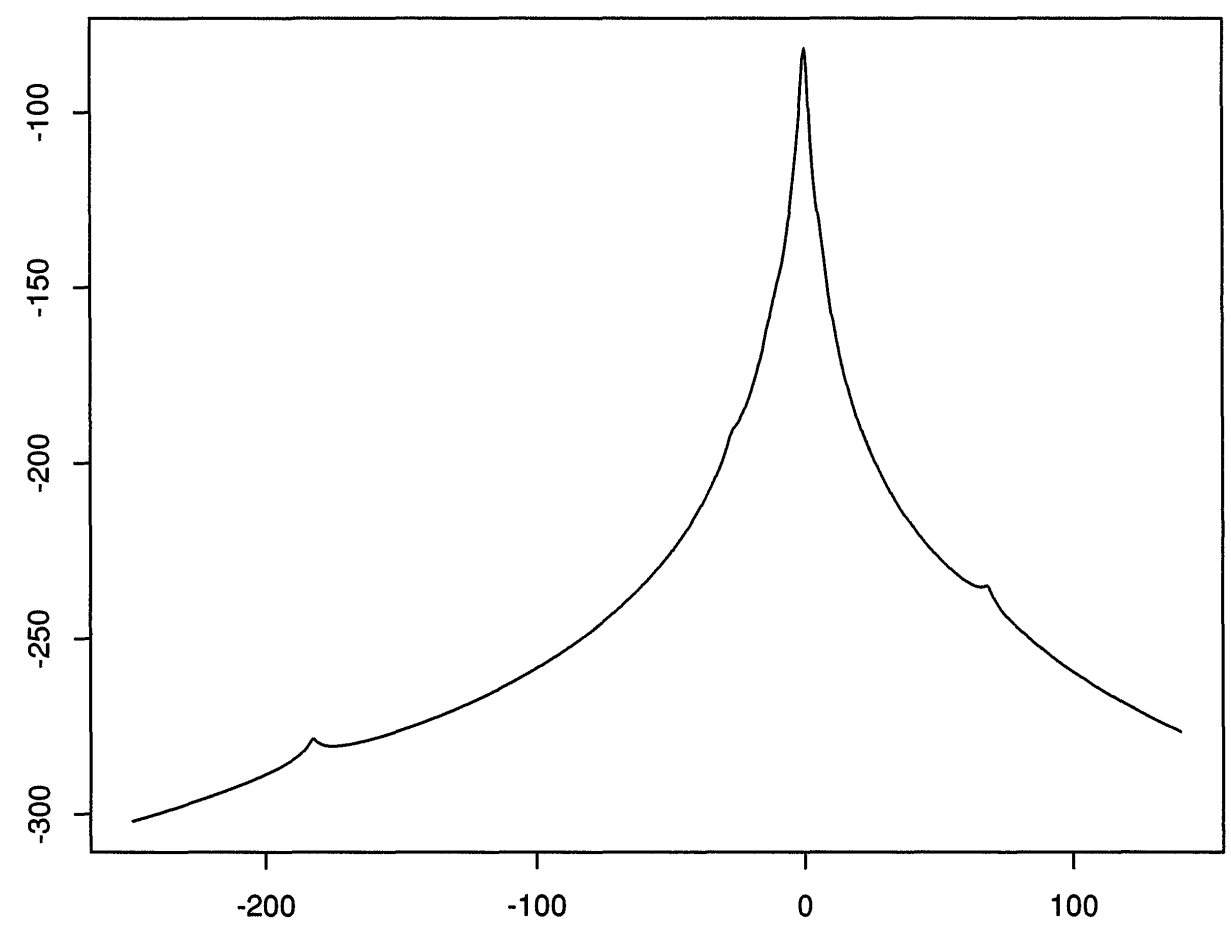
\includegraphics[width=0.72\textwidth]{figures/07-cauchy-log-likelihood.png}
  \caption{Cauchy 位置模型的对数似然函数。图片来自 \cite{vandervaart1998}, p.~74}
  \label{fig:ch7:cauchy-loglik}
\end{figure}

可见有三个局部极大值点，不过全局最大值点是最接近参数真值 0 的，而其它两个则离得很远。关于这个问题，\cite{reeds1985} 曾证明：除了全局最大值的那个点外，其它的``假''局部极大值的个数渐近服从 $\mathrm{Poisson}(1/\pi)$ 分布。


面对 Cauchy 似然方程多根的问题，有一个更加实用的策略，称作\textbf{\emph{单步 MLE}} (One-Step MLE)，其基本思路是利用 Newton 法对一个现有估计进行一步下降：

\begin{enumerate}
\def\labelenumi{\arabic{enumi}.}
\tightlist
\item
  首先选择一个初始的鲁棒估计 $\widehat\theta_0$ ，如样本中位数；
\item
  对 $\widehat\theta_0$ 进行一步 Newton-Raphson 更新： \[ \hat{\theta}_n := \hat{\theta}_0 - \left( \ell_n''(\hat{\theta}_0) \right)^{-1} \ell_n'(\hat{\theta}_0) \]这就是单步 MLE。
\end{enumerate}

单步 MLE 完全不关心似然方程到底有几个根，自然不用在意多根问题。可以证明：单步 MLE 可以改进统计量的效率：虽然 $\widehat\theta_0$ 的渐近方差通常不是最优，但只要它是 $\sqrt n$ -相合的，那么 (在适当正则条件下) $\widehat\theta_n$ 就是渐近有效估计。参考 \cite{shao2003} 一书的 Theorem 4.19。

\end{example}

\subsection{渐近正态性}

MLE 不仅是渐近正态的，也是渐近有效的，即其渐近方差可以达到 C-R 下界 $I^{-1}(\theta)$ 。我们来证明此事。

\begin{theorem}[MLE 的渐近正态性]\label{thm:ch7:mle-asymptotic-normality}

设 $X_1,X_2,\dots,X_n \sim P_{\theta_0}$ i.i.d.，参数空间 $\Theta \subset \mathbb{R}$，存在 $\theta_0$ 的开邻域 $\Theta_0$ 满足：

\begin{enumerate}
\def\labelenumi{\arabic{enumi}.}
\tightlist
\item
  $p_{\theta'}(x) > 0$ 对所有 $x$ 和 $\theta' \in \Theta_0$ 成立；
\item
  $p_\theta(x)$ 在 $\Theta_0$ 内三次可微；
\item
  $p_\theta(x)$ 的三次导数可被控制，即：存在 $M(x) \ge 0$，$\mathbb{E}_{\theta_0}[M(X)] < \infty$，且 $\left|\frac{{\rm d}^3}{{\rm d}\theta^3} \log p_{\theta'}(x)\right| \le M(x)$ 对所有 $\theta' \in \Theta_0$ 成立；
\item
  $p_\theta(x)$ 的积分与一阶、二阶导数可交换，即 $\int \frac{{\rm d}^ip_\theta(x)}{{\rm d}\theta^i} \big|_{\theta=\theta_0} \mathrm{d}\mu(x)=0,\  i=1,2$；
\item
  $0 < I(\theta') < \infty$ 对所有 $\theta' \in \Theta_0$ 成立；
\item
  存在 $\theta_0$ 的 MLE $\widehat\theta_n$ 使得 $\widehat\theta_n\overset P\to \theta$ ，且 $\lim\limits_{n\to\infty}P_{\theta_0}\left(\widehat\theta_n\text{ 是似然方程的唯一解 }\right)=1$ ；
\item
  参数族可识别。
\end{enumerate}

则 \[\sqrt{n} \big(\hat{\theta}_n - \theta_0\big) \overset{\rm d}\longrightarrow \mathcal{N}\left(0, I^{-1}(\theta_0)\right)\]
\end{theorem}

\begin{proof}

仍记 $\ell_n(\theta)$ 是对数似然函数，则 $\hat{\theta}_n$ 满足 $\ell_n'(\hat{\theta}_n) = 0$。在 $\theta_0$ 处作 Taylor 展开：

\begin{equation}
\label{eq:ch7:tag-3}
0 = \ell_n'(\theta_0) + \ell_n''(\theta_0)(\hat{\theta}_n - \theta_0) + \frac{1}{2} \ell_n'''(\tilde{\theta}_n) (\hat{\theta}_n - \theta_0)^2
\end{equation}

其中 $\tilde{\theta}_n$ 位于 $\hat{\theta}_n$ 与 $\theta_0$ 之间。

首先，由弱大数律，

\begin{equation}
\label{eq:ch7:tag-4}
\frac1n\ell_n''(\theta_0) = \frac{1}{n} \sum_{j=1}^n \frac{\partial^2}{\partial \theta^2} \log p_{\theta_0}(X_j) \overset{P}{\longrightarrow} \mathbb{E}_{\theta_0}\left[ \frac{\partial^2}{\partial \theta^2} \log p_{\theta_0}(X) \right] = -I(\theta_0)
\end{equation}

这里期望等于 $-I(\theta_0)$ 用到了条件 (4.)。其次，由条件 (3.)，
\[\frac1n|\ell_n'''(\tilde{\theta}_n)| \le \frac{1}{n} \sum_{j=1}^n M(X_j) \overset{P}{\longrightarrow} \mathbb{E}_{\theta_0}[M(X)] < \infty\]
故 $\tfrac1n\ell_n'''(\tilde{\theta}_n) = O_P(1)$。又因 $\hat{\theta}_n - \theta_0 = o_P(1)$，所以

\begin{equation}
\label{eq:ch7:tag-5}
\frac1n(\hat{\theta}_n - \theta_0)^2 \ell_n'''(\tilde{\theta}_n) = (\hat{\theta}_n - \theta_0)o_P(1)
\end{equation}

我们将式~\eqref{eq:ch7:tag-4}、\eqref{eq:ch7:tag-5} 代入式~\eqref{eq:ch7:tag-3}：\[
0=\frac1n\ell'_n(\theta_0)+\big(-I(\theta)+o_P(1)\big)\big(\widehat\theta_n-\theta_0\big)\]
最后，由经典中心极限定理，\[
\frac1{\sqrt n}\ell_n'(\theta_0) = \frac{1}{\sqrt{n}} \sum_{j=1}^n \frac{\partial}{\partial\theta} \log p_{\theta_0}(X_j) \overset{\rm d}\longrightarrow \mathcal{N}\big(0, I(\theta_0)\big)\]
由 Slutsky 定理直接得出\[ \begin{aligned} \sqrt{n}(\hat{\theta}_n-\theta_0) & =I^{-1}(\theta_{0})\frac1{\sqrt{n}}\ell_{n}^{\prime}(\theta_{0})+o_{P}(1)\\ &\overset{\rm d}\to\mathcal N(0,I^{-1}(\theta_{0})) \end{aligned} \]

\end{proof}

\begin{remark}

\begin{itemize}
\tightlist
\item
  这个定理非常经典，在很多教材中都可以见到，例如 \cite{lehmanncasella1998} 一书的 §6.3 之 Theorem 3.10 (pp.~449-450)。
\item
  在多维情况下，条件 (3.) 需改成 $\Bigl|\frac{\partial^3}{\partial\theta_u\partial\theta_v\partial\theta_w}\log p_\theta(x)\Bigr|\le M(x),\quad u,v,w=1,\dots,k$ ；条件 (5.) 改成 Fisher 信息矩阵 $I(\theta)$ 正定且有限。证明思路与一维类似。
\end{itemize}
\end{remark}

但同时，定理~\ref{thm:ch7:score-root-consistency} 和推论~\ref{cor:ch7:mle-consistency} 的条件也是比较苛刻的：它要求密度二阶或三阶可微、MLE 必须是似然方程的唯一根，等等。这些条件在很多实际模型中不一定满足，或者验证起来很麻烦。在参数空间有良好几何结构的时候，这些条件可以放宽，如下

\begin{theorem*}

设 $X_1,X_2,\dots,X_n \sim P_{\theta_0}$ i.i.d.，$\hat{\theta}_n$ 是基于 $n$ 个 i.i.d. 样本的 MLE。假设：

\begin{itemize}
\tightlist
\item
  $\Theta \subset \mathbb{R}^p$ 为紧致凸集，$\theta_0$ 是 $\Theta$ 的内点；
\item
  所有 $x$ ， $\log p_\theta(x)$ 对 $\theta$ 连续可微，导数满足 $\left|\tfrac{\partial \log p_\theta(x)}{\partial \theta}\right| \le L(x)$，其中函数 $L$ 满足 $\mathbb{E}_\theta[L^2(X_1)] < \infty$；
\item
  参数族可识别。
\end{itemize}

那么 $\widehat\theta_n\overset{P}\to \theta_0$ 。

如果再加上

\begin{itemize}
\tightlist
\item
  $I(\theta)$ 正定且对 $\theta$ 连续。
\end{itemize}

则
\[\sqrt{n}(\hat{\theta}_n - \theta_0) \overset{\rm d}\longrightarrow \mathcal{N}\left(0, I^{-1}(\theta_0)\right)\]

% 最后，关于 MLE 的渐近性质，读者亦可参考笔者基于陈希孺教材整理的笔记，

% \href{https://zhuanlan.zhihu.com/p/1908156011602224244}{数理统计 (15) : 极大似然估计 - 中 - MLE 的相合性}

% \href{https://zhuanlan.zhihu.com/p/1909962170453726655}{数理统计 (16) : 极大似然估计 - 下 - MLE 的渐近正态性}

\end{theorem*}

这个结论来自 \cite{bijma2017} 一书的 Lemma 5.14 和 Theorem 5.9。
\section{基于似然的假设检验}

\subsection{Wald 检验}

基于 MLE 渐近正态性，可以直接构造参数 $\theta$ 的置信域。设 $\Theta\subset\mathbb R^k$ ， $I(\theta)$ 连续，则有
\[\sqrt{n}I^{1/2}(\hat{\theta}_n)(\hat{\theta}_n - \theta) \overset{\rm d}\longrightarrow \mathcal{N}_k(0, \mathbf I_k)\]
从而我们有渐近 $1-\alpha$ 置信域
\[I_\alpha(B_\alpha) = \left\{ \theta : \sqrt{n} I^{-1/2}(\hat{\theta}_n)(\hat{\theta}_n - \theta) \in B_\alpha \right\},\]
其中集合 $B_\alpha \subset \mathbb{R}^k$ 满足 $\mathbb{P}(\mathcal{N}_k(0, \mathbf I_k) \in B_\alpha) = 1-\alpha$。

进一步，对于假设检验 $H_0: \theta = \theta_0$，\textbf{\emph{Wald 检验}} 统计量为
\[W_n := n (\hat{\theta}_n - \theta_0)^\top I(\theta_0) (\hat{\theta}_n - \theta_0) \overset{\rm d}\longrightarrow \chi^2_k\]
拒绝域为 $W_n > \chi^2_k(1-\alpha)$。这个方法非常简单直接，并且不需要一个主观选择的 $B_\alpha$ 。

\subsection{似然比检验}

考虑复合假设
\[
H_0:\theta\in\Theta_0
\qquad\text{对}\qquad
H_1:\theta\in\Theta\setminus\Theta_0.
\]
令 $\hat{\theta}_n$ 为整个参数空间 $\Theta\subset\mathbb R^k$ 上的``全局 MLE''，$\tilde{\theta}_n$ 为 $\Theta_0$ 约束下的``受限 MLE''。定义\textbf{\emph{似然比}} (Likelihood Ratio, LR) 检验统计量为
\[\mathrm{LR}_n :=-2\log\frac{\max_{\theta\in\Theta_0 }\prod_{j=1}^np_{\theta}(X_j)}{\max_{\theta\in\Theta}\prod_{j=1}^np_{\theta}(X_j)}= -2 \log \frac{L_n(\tilde{\theta}_n)}{L_n(\hat{\theta}_n)} = 2 \big( \ell_n(\hat{\theta}_n) - \ell_n(\tilde{\theta}_n) \big)\]
其中 $X_1,\dots,X_n\sim P_\theta$ 是 i.i.d. 样本， $L_n(\theta)$ 和 $\ell_n(\theta)$ 分别是基于这些样本的似然函数和对数似然函数。直观上，若 $H_0$ 成立，则加上约束不应使似然下降太多；若 $\mathrm{LR}_n$ 过大，则倾向于拒绝 $H_0$。似然比、Wald 与 Lagrange 乘子检验的几何关系如图~\ref{fig:ch7:likelihood-tests-geometry} 所示。

\begin{figure}[htbp]
  \centering
  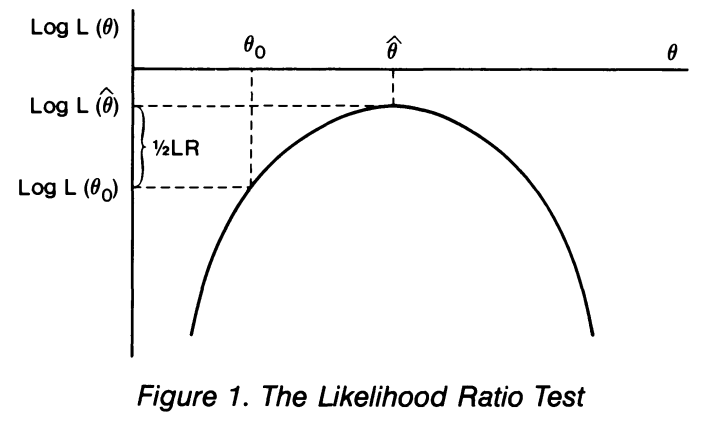
\includegraphics[width=0.78\textwidth]{figures/07-likelihood-tests-geometry.png}
  \caption{似然比、Wald 与 Lagrange 乘子检验的几何关系。图片来自 \cite{buse1982}}
  \label{fig:ch7:likelihood-tests-geometry}
\end{figure}

我们先证明一个辅助引理，

\begin{lemma}[似然比统计量的二次型展开]
\label{lem:ch7:likelihood-ratio-expansion}

设参数空间 $\Theta \subset \mathbb{R}^k$，在定理~\ref{thm:ch7:mle-asymptotic-normality} 的正则条件下，有
\[\begin{aligned} 2(\ell_n(\widehat\theta_n)-\ell_n(\theta_0))&=n(\widehat\theta_n-\theta_0)^\top I(\theta_0)(\widehat\theta_n-\theta_0)+o_P(1)\\ &=\frac1n\ell_n'(\theta_0)^\top I(\theta_0)^{-1}\ell'_n(\theta_0)+o_P(1) \end{aligned}\]
\end{lemma}

\begin{proof}

先证明第一个等式，我们主要利用 $\widehat{\theta}_n$ 是真实参数 $\theta_0$ 的 $\sqrt{n}$‑相合估计，即， $\sqrt n(\widehat\theta_n-\theta_0)=O_P(1)$ 。根据 Taylor 展开：
\[\begin{aligned} 2(\ell_n(\theta_0)-\ell_n(\widehat\theta_n)) &= 2\underbrace{\ell_n'(\widehat\theta_n)^\top (\theta_0-\widehat\theta_n)}_{=0}       +(\theta_0-\widehat\theta_n)^\top \ell_n''(\widehat\theta_n)(\theta_0-\widehat\theta_n) \\ &\quad + \frac13\underbrace{ \sum_{u=1}^k\sum_{v=1}^k\sum_{w=1}^k \frac{\partial^3 \ell_n(\widehat\theta_n)}{\partial\theta_u\partial\theta_v\partial\theta_w}      (\theta_{0u}-\widehat\theta_{nu})(\theta_{0v}-\widehat\theta_{nv})(\theta_{0w}-\widehat\theta_{nw})}_{O_P(n)\cdot O_P(n^{-1/2})\cdot O_P(n^{-1/2})\cdot O_P(n^{-1/2}) = O_P(n^{-1/2}) = o_P(1)} \\      &=(\theta_0-\widehat\theta_n)^\top \ell_n''(\widehat\theta_n)(\theta_0-\widehat\theta_n)+o_P(1)\\      &=-n(\theta_0-\widehat\theta_n)^\top I(\theta_0)(\theta_0-\widehat\theta_n)+o_P(1) \end{aligned}\]
最后一个等号是因为 $\frac1n\ell''(\widehat\theta_n)\overset P\to -I(\theta_0)$ ，从而 $\ell''_n(\theta)=-nI(\theta_0)+o_P(n)$ 。

再证明第二个等式，思路和定理~\ref{thm:ch7:mle-asymptotic-normality} 的证明差不多，由 Taylor 展开 \[ 0=\ell'_n(\widehat\theta_n)=\ell'_n(\theta_0)+\ell_n''(\theta^*)(\widehat\theta_n-\theta_0) \]其中 $\theta^*$ 位于 $\widehat\theta_n$ 和 $\theta_0$ 之间，再利用 $\frac1n\ell''(\theta^*)\overset P\to -I(\theta_0)$ 可知
\[
\sqrt n(\widehat\theta_n-\theta_0)
=I^{-1}(\theta_0)\frac1{\sqrt n}\ell_n'(\theta_0)+o_P(1).
\]
代入第一个等式即可。

\end{proof}

当 $H_0$ 成立时，由于 $\widehat\theta_n-\tilde\theta_n=O_P(n^{-1/2})$ ，因此引理~\ref{lem:ch7:likelihood-ratio-expansion} 的推导也完全成立，我们有 $\mathrm{LR}_n=n(\widehat\theta_n-\widetilde\theta_n)^\top I(\theta_0)(\widehat\theta_n-\widetilde\theta_n)+o_P(1)$ 。这说明 $\mathrm{LR}_n$ 可以（渐近地）看作是对 $\widehat\theta_n$ 和 $\widetilde\theta_n$ 的、用 FI 加权的距离度量。

为研究似然比的渐近分布，我们需要结构化的 $\Theta_0$。假定 $\Theta_0$ 可通过 $r$ 维参数 $a$ 光滑地嵌入原参数空间，这是在说：存在 $g: \mathbb{R}^r \to \mathbb{R}^k$ 使得 $\Theta_0 = \{ g(a) : a \in A \}$，其中 $g$ 二阶连续可微、 $A\subset\mathbb R^r$ ，且真实参数 $\theta_0 = g(a_0)$ ， $a_0$ 为 $A$ 的内点。 $g$ 的可微性保证了 $\Theta_0$ 的局部线性性，这在后面 Wilks 定理的证明中是十分重要的。

这也等同于说，$\Theta_0$ 可由 $k-r$ 个光滑约束 $R(\theta)=0$ 表出，其中 $R:\Theta\to\mathbb R^{k-r}$ ；由于原参数空间是 $k$ 维的，而对 $\Theta_0$ 施加的限制抹除了 $r$ 个自由度，直觉上不难想到，其渐近分布是来自于剩下 $k-r$ 个自由度的。

\begin{theorem}[Wilks 定理]
\label{thm:ch7:wilks}

在上述结构及定理~\ref{thm:ch7:mle-asymptotic-normality} 的正则条件下，当 $H_0$ 成立时，
\[\mathrm{LR}_n \overset{\rm d}\longrightarrow \chi^2_{k-r}\]
\end{theorem}

\begin{proof}

首先，对于全局 MLE，用引理~\ref{lem:ch7:likelihood-ratio-expansion} 可得

\begin{equation}
\label{eq:ch7:tag-6}
2 \big( \ell_n(\hat{\theta}_n) - \ell_n(\theta_0) \big) = \frac{1}{n} \ell'_n(\theta_0)^\top I^{-1}(\theta_0) \ell'_n(\theta_0)  + o_P(1)
\end{equation}

对于受限 MLE $\widetilde{\theta}_n = g(\widehat a_n)$，以 $a$ 为参数，类似可得

\begin{equation}
\label{eq:ch7:tag-7}
2 \big( \ell_n(g(\widehat a_n)) - \ell_n(g(\phi_0)) \big) = \frac{1}{n} \left( \frac{\mathrm{d} \ell_n(g(a_0))}{\mathrm{d} a} \right)^\top \widetilde{I\ }^{-1}\!(a_0) \left( \frac{\mathrm{d} \ell_n(g(a_0))}{\mathrm{d}a} \right) + o_P(1)
\end{equation}

其中 $\widetilde{I\ }\!(a_0) := \mathbb{E}_{\theta_0}\left[ \frac{\partial \log p_{g(a)}(X)}{\partial a} \frac{\partial \log p_{g(a)}(X)}{\partial a}^\top \right]$ 是参数 $a_0$ 的 $r\times r$Fisher 信息矩阵。由求导的链式法则，
\[\begin{aligned}\frac{\mathrm{d}\ell_n(g(a_0))}{\mathrm{d} a} &= g'(a_0)^\top \ell'_n(\theta_0)\\ \widetilde{I\ }\!(a_0) &= g'(a_0)^\top  I(\theta_0)g'(a_0)\end{aligned}\]
这里 $g'(a_0)$ 为 $k \times r$Jacobian 矩阵。

我们将式~\eqref{eq:ch7:tag-6}、式~\eqref{eq:ch7:tag-7} 两式作差，得到
\[\begin{aligned} \mathrm{LR}_n &= 2 (\ell_n(\hat{\theta}_n) - \ell_n(\tilde{\theta}_n)) \\ &= \frac{1}{n} \ell'(\theta_0)^\top \big( I^{-1}(\theta_0) - g'(a_0)(g'(a_0) I(\theta_0) g'(a_0)^\top)^{-1} g'(a_0) ^\top \big) \ell'(\theta_0)+ o_P(1) \end{aligned}\]
令 $Z_n := \frac{1}{\sqrt{n}} I^{-1/2}(\theta_0) \ell'_n(\theta_0)$，由 CLT 有 $Z_n \overset{\rm d}\longrightarrow Z \sim \mathcal{N}_k(0,\mathbf I_k)$。于是
\[\mathrm{LR}_n = Z_n^\top \, M \, Z_n + o_P(1) \overset{\rm d}\longrightarrow Z^\top M Z\]
其中 \[ M := \mathbf I_k - I(\theta_0)^{1/2} g'(a_0) (g'(a_0)^\top I(\theta_0) g'(a_0))^{-1} g'(a_0)^\top I^{1/2}(\theta_0) \]直接验证易知 $M$ 是对称的幂等矩阵（$M^2 = M$），且迹为
\[\begin{aligned} \mathrm{tr}(M) &=\mathrm{tr}(\mathbf I_k) - \mathrm{tr}\big( (g'(a_0)^\top I(\theta_0) g'(a_0))^{-1} g'(a_0)^\top I(\theta_0) g'(a_0)\big)\\ \\ &=k-\mathrm{tr}\Big(\underbrace{\widetilde{I\ }^{-1}\!(a_0)\widetilde{I\ }\!(a_0)}_{\mathbf I_r}  \Big)\\ &=k-r \end{aligned}\]
故 $\mathrm{LR}_n\overset{\rm d}\to\chi^2_{k-r}$ ，如所欲证。

\end{proof}

根据定理~\ref{thm:ch7:wilks}，可以构造近似水平为 $\alpha$ 的接受域 $\{\mathrm{LR}_n\le \chi^2_{k-r}(1-\alpha)\}$，其中 $\chi^2_{k-r}(1-\alpha)$ 代表 $\chi^2$ 分布 $\chi^2_{k-r}$ 的 $1-\alpha$ 分位数。

\begin{remark}

\begin{itemize}
\tightlist
\item
  这个证明也很经典，例如可见 \cite{serfling1980} 的 4.4 节、\cite{shao2003} 一书的 Theorem 6.5 或者 \cite{chenxiru2009} 一书的定理 6.1 等。
\item
  在复合假设下，我们也可以把之前简单假设下的 Wald 检验进行修改，由 Delta 方法： \[ \sqrt nR(\widehat\theta_n)\overset{\rm d }\longrightarrow\mathcal N_{k-r}\big(0,R'(\theta_0)I^{-1}(\theta_0)R'(\theta_0)^\top\big) \]可以得到如下 \emph{Wald 检验}统计量： \[ W_n:=nR(\widehat\theta_n)^\top\big(R'(\widehat\theta_n)I^{-1}(\widehat\theta_n)R'(\widehat\theta_n)^\top\big)^{-1}R(\widehat\theta_n) \]此外还有 \emph{Rao's Score 检验}，其形式来自引理~\ref{lem:ch7:likelihood-ratio-expansion} 的第二个等式，我们用\emph{插入原则} (plug-in principle)，对 $I(\theta_0)$ 用 $I(\widetilde\theta_n)$ 估计之，对 $\ell'(\theta_0)$ 用 $\ell'(\widetilde\theta_n)$ 估计之，即可得到如下检验统计量
  \[
  R_n:=\frac1n\ell'_n(\widetilde\theta_n)^\top
  I^{-1}(\widetilde\theta_n)\ell'_n(\widetilde\theta_n).
  \]
  读者可以验证：似然比检验、Wald 检验、Rao's Score 检验，三者在原假设下是渐近等价的。相比于似然比检验统计量要算两个 MLE，Wald 检验只看全参数空间下的 MLE，而 Rao's Score 检验只看受限参数空间的 MLE，因而二者在计算上更加简单。
\item
  一个例子是存在讨厌参数 (Nuisance Parameter) 的假设检验问题。设参数分为 $\theta = (\beta, \gamma)$，其中 $\beta$ 是我们感兴趣的参数，$\gamma$ 是讨厌参数。我们关心检验
  \[
  H_0:\beta=\beta_0
  \qquad\text{对}\qquad
  H_1:\beta\ne\beta_0.
  \]
  设全参数空间的 MLE 为 $\hat\theta_n = (\hat\beta_n, \hat\gamma_n)$，而受限于 $H_0$ 的 MLE 为 $\tilde\gamma_n = \operatorname*{\arg\sup}\limits_{(\beta_0,\gamma)\in\Theta} \ell_n(\beta_0,\gamma)$ ，后者也被称作是 $\beta_0$ 的轮廓似然 (Profile Likelihood
  % 例如可见 \url{https://www.zhihu.com/question/310585422}
  )。在正则条件满足时，有似然比统计量\[ \mathrm{LR}_n(\beta_0) = 2\bigl( \ell_n(\hat\beta_n, \hat\gamma_n) - \ell_n(\beta_0, \tilde\gamma_n) \bigr) \]设 $\Theta = \Theta_\beta \oplus \Theta_\gamma$ （ $\beta,\gamma$ 的参数空间正交），且 $\dim\Theta=k$ 、 $\dim\Theta_\gamma = r$。那么根据定理~\ref{thm:ch7:wilks}，在 $H_0$ 下\[ LR_n(\beta_0) \overset{\rm d}\longrightarrow \chi^2_{k-r} \]从而，我们有近似的接受域 $\{\beta:\mathrm{LR}_n(\beta)\le \chi^2_{k-r}(1-\alpha)\}$ 。
\end{itemize}
\end{remark}

\begin{example}[Wilks 定理的反例]
如果正则条件不满足，则定理~\ref{thm:ch7:wilks} 的极限分布可能不适用。如，设 $X_i \sim \mathcal U(0,\theta)$，由于参数位于密度支撑集的边界，这违背了定理~\ref{thm:ch7:mle-asymptotic-normality} 的第 (1.) 条。我们想检验
\[
H_0: \theta = \theta_0\quad \iff\quad H_1:\theta\ne \theta_0,
\]
其中 $\theta_0>0$ ；由于 MLE 为 $X_{(n)}$，且原假设下的似然函数为 $L_n(\theta_0)=\theta_0^{-n}$ ，则似然比统计量为
\[
\mathrm{LR}_n = -2n \log\frac{X_{(n)}}{\theta_0}\quad \text{ 当 }X_{(n)}\le \theta_0.
\]

当原假设成立时，周知 \[ Y_n:=n\frac{\theta_0-X_{(n)}}{\theta_0}\overset{\rm d}\to\mathrm{Exp}(1)\overset{\rm d}=\frac12\chi_2^2 \]从而 \[ \mathrm{LR}_n=-2n\log\left(1-\frac{Y_n}n\right)=2Y_n+o_P(1)\overset{\rm d}\to \chi_2^2 \]极限分布为 $\chi^2_2$，自由度是不符合定理~\ref{thm:ch7:wilks} 的。


\end{example}

\subsection{Bartlett 校正}

虽然 Wilks 定理给出了 $\mathrm{LR}_n$ 的极限分布，但在有限样本下，其分布毕竟还是与 $\chi^2_{k-r}$ 有差距，例如相比于 $\mathbb{E}[\chi^2_{k-r}]=k-r$ ， $\mathbb{E}[\mathrm{LR}_n]$ 往往偏大。Bartlett 在 1937 年提出了 ``\textbf{\emph{Bartlett 较正}} (Bartlett correction)''，其出发点就是希望在有限样本下校正此类偏差，从而改进似然比检验。其核心观察在于， $\mathrm{LR}_n$ 的期望可以展开为
\[
\mathbb{E}[\mathrm{LR}_n] = (k-r) + \frac{b_1}{n} + o(n^{-1}) = (k-r)\left(1 + \frac{b}{n} + o(n^{-1})\right).
\]

其中 $b$ 或 $1 + \frac{b}{n}$ 被称为 \textbf{\emph{Bartlett 因子}} (Bartlett factor)。这样一来， $\tfrac{\mathrm{LR}_n}{1+b/n}$ 就十分符合我们的要求：它的期望与目标极限分布 $\chi^2_{k-r}$ 之间仅相差 $o(n^{-1})$ 。

当然， $b$ 本身取决于 $\theta_0$ ，也是未知的；若能得到 $b$ 的一个相合估计 $\widehat{b}_n \stackrel{P}\to b$，则可以定义 Bartlett 校正的似然比统计量 
$$\mathrm{LR}_{n, bc} := \frac{\mathrm{LR}_n}{1 + \hat{b}_n / n}$$
由 Slutsky 定理，其仍满足 $\mathrm{LR}_{n, bc}\overset{\rm d}\to \chi^2_{k-r}$ 。

Bartlett 校正 $\mathrm{LR}_{n, bc}$ 真的能比 $\mathrm{LR}_{n}$ 取得更好的近似吗？这里更进一步地探讨一下：首先 Wilks 定理告诉我们，在原假设下， 

$$\lim_{n \to \infty} P(\mathrm{LR}_n \le x) = P(\chi^2_{k-r} \le x)$$
即逼近误差为 $o(1)$；若进一步使用 Edgeworth 展开（需要更强的矩条件和尾部性质，如 \emph{Cramér 条件}，见第~\ref{ch:characteristic-functions}~章），实际上可以证明 \cite{hayakawa1977,chandraghosh1979}：

$$P(\mathrm{LR}_n \le x) = P(\chi^2_{k-r} \le x) + O(n^{-1})$$

对于检验简单原假设 $H_0: \theta = \theta_0$ 的情形， $\mathrm{LR}_n\overset{\rm d}\to\chi_k^2$ ，一般有\[
\mathbb{E}[\mathrm{LR}_n(\theta_0) ] = k\left(1+\frac\beta n\right)+O(n^{-2})\]
即期望仅在首阶与 $\chi^2_k$ 的均值 $k$ 一致。更精细地 \cite{barndorffnielsencox1984,barndorffnielsenhall1988}：\[
P(\mathrm{LR}_n(\theta_0) \le x) = P(\chi^2_k \le x) - \beta x g_k(x) n^{-1} + O(n^{-2})\]
其中 $g_k$ 是 $\chi^2_k$ 的密度函数；此时如果采用 Bartlett 校正，那么\[
P\left( \frac{\mathrm{LR}_n}{1 + \beta n^{-1}} \le x \right) = P( \chi^2_{k} \le x ) + O(n^{-2})\]
且当 $\widehat\beta_n$ 是 $\beta$ 的 $\sqrt n$ -相合估计时，
\[
P\left( \frac{\mathrm{LR}_n}{1 + \hat{\beta} n^{-1}} \le x \right) = P( \chi^2_{k} \le x ) + O(n^{-3/2}).
\]

这从理论上表明，Bartlett 校正确实可以将似然比统计量分布逼近精度提高。

\nocite{vandervaart1998,serfling1980,shao2003}
\chapterreferences
\end{refsection}

\begin{refsection}
\chapter{经验似然}\label{ch:empirical-likelihood}
% Generated from: Zhihu/专栏：概率与统计/渐近统计 (8)：经验似然_金鱼马_2026-06-07.md
\section{经验似然的基本概念}

设 $\mathbb{R}^k$ 上的随机变量 $X_1, \dots, X_n$ 是来自某未知分布 $P$ 的独立同分布 (i.i.d.) 样本，记 $F$ 是其分布函数，我们很自然地定义\textbf{\emph{非参数似然函数 }} (nonparametric likelihood) 为
\[L(F) := \prod_{i=1}^n P(X = X_i) = \prod_{i=1}^n \bigl(F(X_i) - F(X_i -)\bigr)\]
这里 $X_i-$ 表示逐分量的左极限。这个定义直接对应``观测到当前样本的概率''。显然，若 $F$ 是一个连续分布，则 $L(F)=0$；只有那些``在每个观测值上都赋予正概率''的离散分布，才可能具有正的非参数似然。

我们想知道，在所有可能的分布中，哪个会使这个似然达到最大。这个问题的答案其实也是简单的，

\begin{theorem}[Kiefer--Wolfowitz]\label{thm:ch8:empirical-likelihood}

设 $X_1, \dots, X_n \sim F_0$i.i.d.，记 $F_n$ 为其经验分布函数 (ECDF) ：
\[F_n(t):=\frac1n\sum_{i=1}^n\mathbb I(X_i< t)\]
而 $F$ 为任意累积分布函数。若 $F \neq F_n$，则 $L(F) < L(F_n)$。

\end{theorem}

\begin{proof}

记 $p_i = F(X_i) - F(X_i -)$ 代表 $F$ 在样本 $X_i$ 上的概率质量，显然若有某个 $p_i = 0$ 则 $L(F) = 0$，命题已然成立。否则，由 AM-GM 不等式，\[
\frac{L(F)}{L(F_n)} = \frac{\prod_{i=1}^np_i}{\prod_{i=1}^n(1/n)}=\prod_{i=1}^nnp_i\le \left(\sum_{i=1}^np_i\right)^n\le 1\]
因此 $L(F) < L(F_n)$。

\end{proof}

这表明经验分布函数 $F_n$ 最大化非参数似然，也就是\textbf{\emph{非参数极大似然估计}} (NPMLE)。在定理~\ref{thm:ch8:empirical-likelihood} 的证明中，\[
R(F) := \frac{L(F)}{L(F_n)}=\prod_{i=1}^nnp_i\]
称作\textbf{\emph{经验似然比}} (empirical likelihood ratio)，则 $R(F)\le 1$ 恒成立。这个量用于衡量：相比于无约束的最优解 $F_n$ ，我们选择的 $F$ 能有多好。不像参数似然比，非参数似然比里不包含任何未知参数。

定理~\ref{thm:ch8:empirical-likelihood} 还可以从另一个角度证明：考虑满足 $L(F) > 0$ 的那些 $F$，令 $c \in (0, 1]$，\[
\mathcal{F}(c) := \left\{F\text{ 是分布函数} : p_i = F(X_i)-F(X_i-) > 0,\; i=1,\dots,n,\; \sum_{i=1}^n p_j = c \right\}\]
利用 Lagrange 乘子法求 $\log L(F)$ 在 $F \in \mathcal{F}(c)$ 上的最大化问题。令\[
H(p_1, \dots, p_m, \lambda) := \sum_{i=1}^n \log p_i + \lambda \left( \sum_{i=1}^n p_i - c \right)\]
其中 $\lambda$ 是 Lagrange 乘子，求偏导得\[
\frac{\partial H}{\partial \lambda} = \sum_{i=1}^n p_j - c = 0, \quad \frac{\partial H}{\partial p_i} = \frac{1}{p_i} + \lambda = 0,\; i = 1, \dots, n\]
解得 $\widehat p_i =-1/\lambda= c/n$，$i = 1, \dots, n$；容易验证此时 $H$ 确实达到最大。因此
\[\max_{F \in \mathcal{F}(c)} L(F) = (c/n)^n\]
上式当 $c=1$ 时达到最大，对应的最大值点为 $\widehat p_i = 1/n$ ，此时自然对应经验分布。

使用 Lagrange 乘子法的好处在于，它可以灵活地增加对分布的约束。假设我们感兴趣的参数 $\theta$ 是分布 $F$ 的一个泛函 $T(F)$（例如均值 $\mu = \int x\, dF(x)$、方差、分位数等），Owen 定义了如下 \textbf{\emph{剖面经验似然比}} (profile empirical likelihood ratio) 统计量：\[
\begin{aligned}\mathcal{R}(\theta) &:= \sup_F \left\{ R(F)=\frac{L(F)}{L(F_n)}:T(F)=\theta,F\ll F_n \right\} \\ &=\sup_F\left\{\prod_{i=1}^nnp_i:T(F)=\theta,p_i\ge 0,\sum_{i=1}^np_i=1\right\} \end{aligned}\]
这个定义要求 $F$ 在满足约束 $T(F)=\theta$ 下使得经验似然比达到最大，这是可以利用 Lagrange 乘子法来求解的。定义里只考虑所有质量都集中在样本上的分布 $F$ ，即 $F\ll F_n$ ，是因为只有这样的 $F$ 才有可能让经验似然比达到极大。

基于 (剖面) 经验似然比，作 $T(F)$ 的区间估计、假设检验或其它统计推断问题，是经验似然方法的基本思想。例如，对于要检验的参数 $\theta_0$ 和某临界值 $r_0$ ，如果 $\mathcal R(\theta_0)<r_0$ 就拒绝 $H_0:\theta=\theta_0$ 的假设；而经验似然置信域为 $\{\theta:\mathcal R(\theta)\ge r_0\}$随之而来的一个问题是如何确定临界值 $r_0$ ，这一问题归结为求 $\mathcal R(\theta)$ 的渐近分布。大家知道参数似然比一个重要的特性是似然比的对数是渐近服从 χ² 分布的，即所谓 Wilks 定理 ， 幸运的是，经验似然比也有相同的特性，这一特性形成了经验似然统计推断的基础。对此，我们将在下一节介绍简单而且最重要的总体均值推断。

\section{均值的经验似然}

\subsection{Lagrange 乘子法求解}

考虑最简单的情形：对 $\mathbb R^k$ 上的随机变量 $X$，我们想对其均值 $\mu = \mathbb{E}[X]$ 进行统计推断。抽取 i.i.d. 样本 $X_1,\dots,X_n$ ，那么在上述框架下，我们需要求解：\[
\begin{aligned} \max_{p_1,\dots,p_n} &\quad \prod_{i=1}^n n p_i, \\ \text{s.t.} &\quad p_i \ge 0,\; \sum_{i=1}^n p_i = 1,\; \sum_{i=1}^n p_i X_i = \mu \end{aligned}\]
利用 Lagrange 乘子法，记\[
H(p_1,\dots,p_n, \lambda_n, \gamma_n) = \sum_{i=1}^n \log(n p_i) - n\lambda_n^\top \sum_{i=1}^n p_i (X_i - \mu) + \gamma_n\left(\sum_{i=1}^n p_i - 1\right)\]
（这里第二项的乘子写作 $n\lambda_n$ ，纯粹是为了后面计算上的方便。）

对 $p_i$ 求偏导并置零：\[
\frac{\partial H}{\partial p_i} = \frac{1}{p_i} - n\lambda_n^\top (X_i - \mu) + \gamma_n = 0\]
即， $1-n\lambda_n^\top p_i(X_i - \mu)+\gamma_n p_i=0$ 对每个 $i$ 成立，求和得到 $n-n\lambda_n^\top\underbrace{\sum_{i=1}^n p_i(X_i - \mu)}_{=0}+\gamma_n\underbrace{\sum_{i=1}^np_i}_{=1}=0\enspace \implies \enspace \gamma_n=-n$ 于是\[
p_i = \frac{1}{n}\frac{1}{1 + \lambda_n^\top (X_i - \mu)}\]
其中的 Lagrange 乘子 $\lambda_n=\lambda_n(\mu)$ 由约束 $\sum_{i=1}^n p_i (X_i - \mu) = 0$ 所隐式决定，即：\[
\label{eq:ch8:tag-1}
\frac{1}{n}\sum_{i=1}^n \frac{X_i - \mu}{1 + \lambda_n^\top (X_i - \mu)} = 0\]
可见，最优权重恰为平均权重 $1/n$ 乘以一个与 $\lambda_n$ 有关的因子。

\begin{remark}
如果方程~\eqref{eq:ch8:tag-1} 无解，则经验似然无定义。后文中我们会讨论方程是否有解的问题。
\end{remark}

如果方程~\eqref{eq:ch8:tag-1} 能解出 $\lambda_n$ ，那么有剖面经验对数似然比\[ \log \mathcal R(\mu)=\sum_{i=1}^n\log np_i=-\sum_{i=1}^n\log(1+\lambda_n^\top (X_i-\mu)) \]

最大化上述 $\log\mathcal R(\mu)$ ，等价于找 \[ \widehat\mu_{\text{MELE}}=\operatorname*{\arg\min}_\mu \sum_{i=1}^n\log(1+\lambda_n^\top(X_i-\mu)) \]这被称作\textbf{\emph{极大经验似然统计量 }} (maximum empirical likelihood estimator, MELE)。在这里，显然让 $\lambda_n=0$ 、 $\mu=\bar{X}$ 可以满足方程~\eqref{eq:ch8:tag-1} ，且让 $\mathcal R(\mu)$ 达到最大值 1，说明没有任何其它条件时， $\bar{X}$ 就是 MELE。

\subsection{经验对数似然比的渐近分布}

我们还可以建立如下的\textbf{\emph{经验对数似然比统计量}} (empirical log-likelihood ratio statistic)：
\[
-2\log \mathcal R(\mu)=2\sum_{i=1}^n\log(1+\lambda_n^\top(X_i-\mu)).
\]

为了分析其渐近分布，我们首先准备两个引理，

\begin{lemma}[样本极大值的阶]\label{lem:ch8:sample-maximum}

设 $X_1,\dots,X_n$ 是 $\mathbb R$ 上的 i.i.d. 随机变量， $\mathbb E[X_1^2]<\infty$ ，记 $M_n:=\max\limits_{1\le i\le n}|X_i|$ ，那么 $M_n=o(n^{1/2})\quad \text{a.s.}$

\end{lemma}

\begin{proof}

由于对每个 $i$ ， $\mathbb E[X_i^2]<\infty$ ，我们有 $\sum_{n=1}^\infty P(X_i^2>n)<\infty$根据 Borel-Cantelli 引理，以概率 1，事件 $\{|X_i|>n^{1/2}\}$ 只对有限多个 $n$ 成立。使用相同的论证可以表明，对任意 $A>0$ ，以概率 1，事件 $\{|X_i|>An^{1/2}\}$ 只对有限多个 $n$ 成立。这意味着 $\limsup_{n\to\infty} \frac{M_n}{n^{1/2}} \le A \quad \text{a.s.}$ 取 $A\downarrow 0$ ， 即得 $\frac{M_n}{n^{1/2}}\to 0\enspace \text{ a.s.}$ 。

\end{proof}

\begin{lemma}[三阶样本矩的阶]\label{lem:ch8:third-sample-moment}

设 $X_1,\dots,X_n$ 是 $\mathbb R$ 上的 i.i.d. 随机变量， $\mathbb E[X_1^2]<\infty$ ，那么
\[
\frac1n\sum_{i=1}^n|X_i|^3=o(n^{1/2})\quad \text{a.s.}
\]

\end{lemma}

\begin{proof}

注意到
\[
\frac1n\sum_{i=1}^n|X_i|^3\le \frac{M_n}{n}\sum_{i=1}^nX_i^2.
\]

由引理~\ref{lem:ch8:sample-maximum}， $M_n=o(n^{1/2})$ a.s.，再由强大数律知 $\frac1n\sum_{i=1}^nX_i^2=O(1)$ a.s.，即证。

\end{proof}

再来解决方程~\eqref{eq:ch8:tag-1} 有解的问题：

\begin{lemma}[经验似然乘子的存在性]\label{lem:ch8:multiplier-existence}

设 $k$ 维随机向量 $X_1,\dots,X_n\sim F_0$ i.i.d. 具有有限均值 $\mu=\mu_0$ 和正定的协方差矩阵 $\Sigma_0$，则以趋于 1 的概率，存在 $\lambda_n$ 满足方程~\eqref{eq:ch8:tag-1} ，且 $\|\lambda_n\|=O_P(n^{-1/2})$

\end{lemma}

\begin{proof}

把样本中心化，记 $Z_i=X_i-\mu_0$ ，其均值为 0、协方差矩阵为 $\Sigma_0=\mathbb{E}[Z_iZ_i^\top]\succ 0$ 。 Lagrange 乘子 $\lambda_n$ 的方程~\eqref{eq:ch8:tag-1} 可以写作

\begin{equation}
\label{eq:ch8:tag-2}
\frac1n\sum_{i=1}^n\frac{Z_i}{1+\lambda_n Z_i}=0
\end{equation}

考虑函数 \[ l(\lambda):=\frac1n\sum_{i=1}^n\log(1+\lambda^\top Z_i) \]那么其一阶和二阶导数分别为
\[\begin{aligned}l'(\lambda) &= \frac{1}{n}\sum_{i=1}^n \frac{Z_i}{1 + \lambda^\top Z_i}\\ l''(\lambda) &= -\frac{1}{n}\sum_{i=1}^n \frac{Z_iZ_i^\top}{(1 + \lambda^\top Z_i)^2} \end{aligned}\]
从而方程~\eqref{eq:ch8:tag-2} 等价于 $l'(\lambda_n)=0$ 。

值得指出的是，如果某个 $\lambda^*$ 满足 $\|\lambda^*\|=O_P(n^{-1/2})$ ，由引理~\ref{lem:ch8:sample-maximum} 有 $\max\limits_{1\le i\le n}\|Z_i\|=o_P(n^{1/2})$ ，所以 ${\lambda^*}^\top Z_i\le \|\lambda^*\|\|Z_i\|=o_P(1)$ ；这说明以趋于 1 的概率，上述导数的分母都趋于 1；特别地，有 $l''(\lambda^*) \overset{P}\to -\Sigma_0$ 。

考虑取 $\lambda = M \Sigma_0^{-1/2} a n^{-1/2}$，其中 $\|a\| = 1$，$M>0$ 为常数。将 $n l(\lambda) - n l(0)$ 展开：
\[\begin{aligned} n l(\lambda) - n l(0)  &= M\sqrt{n}l'(0)^\top \Sigma_0^{-1/2} a + \frac{M^2}{2} a^\top \Sigma_0^{-1/2} l''(\lambda^*) \Sigma_0^{-1/2} a \\ &= M\sqrt{n}l'(0) \Sigma_0^{-1/2} a - \frac{M^2}{2} a^\top a + o_P(1) \\ &\overset{\rm d}\to M a^\top \mathcal{N}_s(0, \mathbf I_s) - \frac{M^2}{2} \end{aligned}\]
其中

\begin{itemize}
\tightlist
\item
  第一行的 $\lambda^*$ 介于 $0$ 和 $\lambda$ 中间 (Lagrange 型余项)；、
\item
  第二行是因为 $l''(\lambda^*) \overset{P}\to -\Sigma_0$ ，从而 $\Sigma_0^{-1/2} l''(\lambda^*) \Sigma_0^{-1/2} \overset{P}\to -\mathbf I_s$ ；
\item
  第三行对 $\textstyle \sqrt nl'(0)=\frac1{\sqrt n}\sum_{i=1}^nZ_i$ 用多元中心极限定理。
\end{itemize}

注意到上式的收敛关于 $\|a\|=1$ 是一致的，设 $W\sim \mathcal{N}_k(0,\mathbf I_k)$ ，由 $a^\top W\le \|a\|\|W\|=\|W\|$ 知
\[\sup_{\|a\|=1} \bigl( n l(M \Sigma_0^{-1/2} a n^{-1/2}) - n l(0) \bigr) \overset{\rm d}\to M \bigl( \|W\| - \tfrac{M}{2} \bigr)\]
由于 $\|W\|$ 是一个有限的随机变量，我们总可以让 $M$ 足够大使得上式以高概率为负值。从而，对于任意 $\epsilon > 0$，当 $M$ 和 $n$ 足够大时，有
\[P\left( \sup_{\|a\|=1} \bigl( n l(M \Sigma_0^{-1/2} a n^{-1/2}) - n l(0) \bigr) < 0 \right) \ge 1 - \epsilon\]
如果 $l(M \Sigma_0^{-1/2} a n^{-1/2}) \le l(0)$ 对任意 $a$ 成立，这等同于说，球面 $\{\lambda = M \Sigma_0^{-1/2} a n^{-1/2} : \|a\| =1\}$ 上的点取值全都不超过球心的点，所以一定在 $l(\lambda)$ 一定在球的内部某点取得局部极大值，该极大值点 $\lambda_n$ 即为方程~\eqref{eq:ch8:tag-1} 的解，且满足 $\|\lambda_n\| = O_p(n^{-1/2})$。

\end{proof}

\begin{remark}

\begin{itemize}
\tightlist
\item
  这里有一个隐含条件：必须保证 $1+\lambda_n^\top Z_i> 0$ 对每个 $i$ 成立，因为 $\textstyle p_i = \frac{1}{n}\frac{1}{1 + \lambda_n^\top Z_i}$ 一定是一个非负数。不过我们在证明过程中看到 $\lambda_n^\top Z_i=o_P(1)$ ，因此对 $n\to\infty$ ，这一隐含条件总是能以趋于 1 的概率满足的。
\item
  如果 $X_1,\dots,X_n$ 是线性无关的，即，样本协方差矩阵 $\frac1n\sum_{i=1}^nZ_iZ_i^\top$ 正定，那么 $l''(\lambda)$ 负定， $l(\lambda)$ 是一个严格凹函数，极大值点 $\lambda_n$ 是唯一的。
\end{itemize}
\end{remark}

\begin{corollary*}
求解方程~\eqref{eq:ch8:tag-1} 等价于如下约束优化问题：
\[\begin{aligned} \operatorname*{\arg\max}_\lambda \enspace &l(\lambda):=\frac1n\sum_{i=1}^n\log(1+\lambda^\top (X_i-\mu))\\ \text{s.t. }&1+\lambda^\top(X_i-\mu)> 0,\enspace i=1,\dots,n \end{aligned}\]\end{corollary*}

由于目标函数是凹函数，该问题可以用 Newton 法高效求解。为了防止算法越出可行域导致 log 无定义，可以用如下``伪 log''函数替代 log： \[ \log_\star(z) := \begin{cases} \log(z), & z \ge 1/n\\ \log(1/n) - 1.5 + 2 n z - \frac{n^2 z^2}{2}, & z \le 1/n \end{cases} \]将约束优化问题改为无约束优化问题。见 Owen \emph{Empirical likelihood} 的 3.14 节。


下面的重要定理表明：尽管我们从非参数的前提出发，但可以得到与参数似然比检验统计量完全相同的渐近分布 。此时，$-2\log\mathcal{R}(\mu_0)$ 充当了一个\emph{非参数枢轴量}(non‑parametric pivot)：要构造 $\mu_0$ 的置信区间，我们只需用到 χ² 分布的分位数。

\begin{theorem}[经验似然的 Wilks 定理]\label{thm:ch8:mean-wilks}

设 $X_1,\dots,X_n\sim F_0$ i.i.d. 具有有限均值 $\mu_0$ 和正定的协方差矩阵 $\Sigma_0$，则当 $n\to\infty$ 时，
\[-2\log\mathcal{R}(\mu_0) \overset{\rm d}\to \chi^2_k\]
\end{theorem}

\begin{proof}

用引理~\ref{lem:ch8:multiplier-existence}，找一个式~\eqref{eq:ch8:tag-2} 的解 $\lambda_n=O_P(n^{-1/2})$ 。利用恒等式 $\textstyle\frac1{1+x}=1-x+\frac{x^2}{1+x}$ ，那么式~\eqref{eq:ch8:tag-2} 还有

\begin{equation}
\label{eq:ch8:tag-3}
\begin{aligned} 0&=\frac{1}{n}\sum_{i=1}^{n}Z_{i}\!\left(1-\lambda_n^\top Z_{i}+\frac{(\lambda_n^\top Z_i)^{2}}{1+\lambda_n^\top Z_{i}}\right)\\[2mm] &=\bar{Z}-\widehat\Sigma_n\lambda_n+\frac{1}{n}\sum_{i=1}^{n}\frac{(\lambda_n^\top Z_i)^2Z_i}{1+\lambda_n^\top Z_i}  \end{aligned}
\end{equation}

其中 $\bar{Z}:=\frac1n\sum_{i=1}^nZ_i$ 、 $\widehat\Sigma_n:=\frac1n\sum_{i=1}^nZ_iZ_i^\top$ 。由大数律， $\widehat\Sigma_n\to \Sigma_0$ a.s.，因此以趋于 1 的概率，样本协方差矩阵 $\widehat\Sigma_n$ 也是正定的（这来自于矩阵特征值的连续性）。

由引理~\ref{lem:ch8:sample-maximum} 和引理~\ref{lem:ch8:third-sample-moment}，可知这里的余项 
$$\frac{1}{n}\sum_{i=1}^{n}\frac{(\lambda_n^\top Z_i)^2Z_i}{1+\lambda_n^\top Z_i} \lesssim \|\lambda_n\|^2\frac1n\sum_{i=1}^n\|Z_i\|^3=O_P(n^{-1})o_P(n^{1/2})=o_P(n^{-1/2})$$

从而，式~\eqref{eq:ch8:tag-3} 给出 $\lambda$ 有如下渐近表示：
\begin{equation}
\label{eq:ch8:tag-4}
\lambda_n = \widehat\Sigma_n^{-1}\bar{Z}+o_P(n^{-1/2})
\end{equation}
（这里 $o_P(n^{-1/2})$ 实际上表达的是``范数为 $o_P(n^{-1/2})$ 的余项''，后文同理。）

另一方面，我们对 $\log(1+\lambda_n^\top Z_i)$ 进行 Taylor 展开：
\begin{equation}
\label{eq:ch8:tag-5}
\begin{aligned} -2\log \mathcal R(\mu_0)&=2\sum_{i=1}^n\log(1+\lambda_n^\top Z_i)\\ &=2\sum_{i=1}^n\left(\lambda_n^\top Z_i-\frac12(\lambda_n^\top Z_i)^2+\eta_i\right) \end{aligned}
\end{equation}
其中余项是 \[ 2\sum_{i=1}^n\|\eta_i\|\lesssim \|\lambda_n\|^3\sum_{i=1}^n\|Z_i\|^3=O_P(n^{-3/2})\cdot no_P(n^{1/2})=o_P(1) \]从而式~\eqref{eq:ch8:tag-5} 给出

\[
-2\log \mathcal R(\mu_0)
=2n\lambda_n^\top\bar{Z}
-n\lambda_n^\top \widehat\Sigma_n\lambda_n+o_P(1).
\]
将式~\eqref{eq:ch8:tag-4} 代入：
\[\begin{aligned} -2\log \mathcal R(\mu_0)&=2n\bar{Z}^\top\big(\widehat\Sigma_n^{-1}\bar{Z}\big)-n \big(\widehat\Sigma_n^{-1}\bar{Z}\big)^\top \widehat\Sigma_n\big(\widehat\Sigma_n^{-1}\bar{Z}\big)+ o_P(1)  \\ &=n\bar{Z}^\top\widehat\Sigma_n^{-1}\bar{Z}+ o_P(1)   \end{aligned}\]
这个 $\bar{Z}^\top\widehat\Sigma_n^{-1}\bar{Z}$ 是什么东西呢？其实在一维情况下，这玩意就是 t-统计量，高维情况下称作 \href{https://en.wikipedia.org/wiki/Hotelling\%27s_T-squared_distribution\#Hotelling_t-squared_statistic}{Hotelling t²}。我们利用
\[
\sqrt n\widehat\Sigma_n^{-1/2}\bar{Z}\overset{\rm d}\to \mathcal N(0,\mathbf I_k),
\]
立即得知
\[
n\bar{Z}^\top\widehat\Sigma_n^{-1}\bar{Z}\overset{\rm d}\to \chi_k^2.
\]
由 Slutsky 定理忽略 $o_P(1)$ 余项，就得到了
\[
-2\log\mathcal R(\mu_0)\overset{\rm d}\to \chi_k^2.
\]

\end{proof}

这一结果可用于 $\mu$ 的假设检验问题，当 $-2\log\mathcal R(\mu_0)>\chi^2(1-\alpha)$ 时拒绝 $H_0:\mu=\mu_0$ 的假设，这就是一个渐近水平为 $\alpha$ 的检验。同时，可以构造渐近 $1-\alpha$ 的置信域为
\[
\{\mu_0 :-2\log \mathcal{R}(\mu_0) \le \chi^2_k(1-\alpha)\}.
\]

利用经验对数似然比统计量为枢轴量有这样几个好处：

\begin{itemize}
\tightlist
\item
  ``让数据自己说话''：经验似然置信域完全由数据本身决定，因此它能够自然地反映出数据中的偏态、重尾等特征。例如，当样本呈现明显的右偏时，置信区间会向左侧更窄、向右侧更宽。
\item
  经验似然在构造过程中隐式地完成了方差尺度的调整（这被称作 studentization），我们不需要像传统方法那样额外插入一个协方差阵 $\Sigma_0$ 的估计量。
\item
  经验似然置信域在光滑的参数重参数化下是不变的。如果我们对参数 $\theta$ 构造了一个置信域，那么在光滑的一一变换 $\phi = g(\theta)$ 下，只需直接映射原区域即可得到 $\phi$ 的置信域；这继承了参数似然的优良性质。
\end{itemize}

最后，还有一个重要的优点是：经验似然区间永远被严格限制在样本点的凸包（convex hull）之内。这意味着估计值绝不会违背逻辑上的自然边界------比如概率不会被估计为负数，方差不会出现负值。例如，设临界值为 $r_0$ ，则均值的经验似然置信域可以写作 

$$\mathtt{CL}_{r_0,n}=\left\{\sum_{i=1}^np_iX_i:\prod_{i=1}^n(np_i)\ge r_0,\ p_i\ge 0,\ \sum_{i=1}^np_i=1\right\}$$

显见，这个置信域完全包含在样本点构成的凸包中。

当处理高维向量（ $\theta$ 的维度远大于样本容量 $n$ ）时，使用经验似然方法推断总体均值通常会遇到困难，原因有二：一是观测值的凸包太小，无法完全覆盖真实均值；二是样本协方差矩阵奇异。这会导致可能不存在以样本点为支撑的离散分布能满足方程~\eqref{eq:ch8:tag-1} 。关于这类高维经验似然的工作，读者可以去参考 Jinyuan Chang（常晋源）的工作。

\subsection{均值作为一种辅助信息}

经验似然方法 的另一重要特性是它能利用辅助信息改进推断。Owen 表明：当抽样分布的某泛函己知时，通过约束经验似然利用这一信息获得改进的推断，可以得到比单纯的经验分布 $F_n$ 更好的效果。例如，假设 $k$ 维随机向量$X_1,\dots,X_n\sim F$ i.i.d.，分布函数 $F$ 未知，但我们已知其有均值 $\mu_0=\mathbb{E}_F[X]$ ，则根据式~\eqref{eq:ch8:tag-1} ，经验似然估计为 
$$\widehat p_i= \frac{1}{n}\frac{1}{1 + \lambda_n^\top (X_i - \mu_0)},\quad \frac{1}{n}\sum_{i=1}^n \frac{X_i - \mu_0}{1 + \lambda_n^\top (X_i - \mu_0)} = 0$$

从 $\widehat p_i$ 的表达式可以看出，在经验分布的基础上，根据 $\mu_0$ 的信息，经验似然估计对样本点重新进行了赋权。其本质是，在满足均值约束 $\sum_{i=1}^np_i(X_i-\mu_0)=0$ 的前提下，寻找一种与均匀权重 $1/n$ ``距离最近''的赋权方式，这里的``距离''指的是 KL-散度： 
$$\mathrm{D}_{\text{KL}}(F_n\|F)=\sum_{i=1}^n(1/n)\log\frac{1/n}{p_i}=-\frac1n\sum_{i=1}^n\log(np_i)$$
我们自然将 
$$\widehat F(t):=\sum_{i=1}^n\widehat p_i\mathbb I(X_i\le t)$$
作为对真实分布 $F$ 的近似。

\begin{theorem}[辅助均值信息下的经验分布]\label{thm:ch8:auxiliary-mean-expansion}

在上述记号下，设协方差矩阵 $\Sigma_0=\mathrm{Var}_F[X]$ 正定，则
\[
\widehat{F}(t) - F(t) = \frac{1}{n}\sum_{i=1}^n \Big(\mathbb I(X_i \le t) - F(t) - (X_i-\mu_0)^\top \Sigma_0^{-1} W(t) \Big) + o_P(n^{-1/2}).
\]

其中 $W(t) := \mathbb{E}[(X-\mu_0) \mathbb I(X \le t)]$。

\end{theorem}

\begin{proof}

记经验分布函数为 $F_n$ ，考察

\begin{equation}
\label{eq:ch8:tag-6}
\begin{aligned} \widehat{F}(t)-F_n(t) &= \frac1n\sum_{i=1}^n \mathbb I(X_i\le t)(n\hat{p}_i-1)\\ &= \frac1n\sum_{i=1}^n \mathbb I(X_i\le t)\left(\frac1{1+\lambda_n^\top(X_i-\mu_0)}-1\right)\\ &= -\frac1n\sum_{i=1}^n \mathbb I(X_i\le t)\,\lambda_n^\top (X_i-\mu_0) + \frac1n\sum_{i=1}^n\mathbb I(X_i\le t)\,\frac{(\lambda_n^\top (X_i-\mu_0))^2}{1+\lambda_n^\top (X_i-\mu_0)} \end{aligned}
\end{equation}
第三行我们再次利用了恒等式 $\textstyle\frac1{1+x}=1-x+\frac{x^2}{1+x}$ 。注意到，这里式~\eqref{eq:ch8:tag-6} 的第二项模长 
$$\|\lambda_n\|^2 \frac1n\sum_{i=1}^n \frac{\|X_i-\mu_0\|^2}{1+\lambda_n^\top (X_i-\mu_0)} = O_P(\|\lambda_n\|^2) = O_P(n^{-1})$$
从而是可以忽略的（并入后面的 $o_P(n^{-1/2})$ 余项）。至于式~\eqref{eq:ch8:tag-6} 的第一项，由大数律，
\[
\widehat W(t)=\frac1n\sum_{i=1}^n\mathbb I(X_i\le t)(X_i-\mu_0)
\overset P\longrightarrow W(t).
\]
因此，式~\eqref{eq:ch8:tag-6} 立即推出
\[
\widehat F(t)-F_n(t)=-\lambda_n^\top W(t)+o_P(n^{-1/2}).
\]
利用前文式~\eqref{eq:ch8:tag-4}，有
\[
\lambda_n=\Sigma_0(\bar X-\mu_0)+o_P(n^{-1/2}),
\]
故
\[\begin{aligned} \widehat{F}(t)-F_n(t) &= -(\Sigma_0^{-1}(\bar X-\mu_0) + o_P(n^{-1/2}))^\top W(t) + o_P(n^{-1/2})\\ &= -(\bar X-\mu_0)^\top \Sigma_0^{-1} W(t) + o_P(n^{-1/2})\\ &=-\frac1n\sum_{i=1}^n(X_i-\mu_0)^\top\Sigma_0^{-1}W(t) \end{aligned}\]
将上式与 \[ F_n(t)-F(t) = \frac1n\sum_{i=1}^n \bigl(\mathbb I(X_i\le t) - F(t) \bigr) \]相加，立即得证。

\end{proof}

对不同的 $t_1,\dots,t_m\in\mathbb R^k$ ， 对 $m$ 维随机向量 $(\mathbb I(X< t_1),\dots,\mathbb I(X< t_m))^\top$ 用多维中心极限定理，有结论： \[ \sqrt n\Big(F_n(t_1)-F(t_1),\dots, F_n(t_m)-F(t_m)\Big)\overset{\rm d}\to \mathcal N_m(0,\Sigma) \]其中 $\Sigma$ 是 $m\times m$ 矩阵，第 $i,j$ 元为 $F(t_i\wedge t_j)-F(t_i)F(t_j)$ ；那么，根据定理~\ref{thm:ch8:auxiliary-mean-expansion} 立即有

\begin{corollary*}
对不同的 $t_1,\dots,t_m\in\mathbb R^k$，$\sqrt n\Big(\widehat F(t_1)-F(t_1),\dots,\widehat F(t_m)-F(t_m)\Big)\overset{\rm d}\to \mathcal N_m(0,\Sigma_u)$，其中 $\Sigma_u:=\Sigma-W^\top\Sigma_0^{-1} W$，$W:=(W(t_1),W(t_2),\dots,W(t_m))$。
\end{corollary*}

可以看出，比于单纯的经验分布 $F_n$ ，在增加了 $\mu=\mu_0$ 这一信息后，我们的估计 $\widehat F$ 成功将渐近方差减小了 $W^\top\Sigma_0 W$ 。

这一例子来自 \cite{shao2003} 一书的 Theorem 5.4。

\section{估计方程}

注意到总体均值 $\mu$ 由下述估计方程确定： $\int(x-\mu)\mathrm dF(x)=0$

一般地 ， 对 $\theta\in\Theta\subset \mathbb R^p$ 、 $X\in\mathbb R^k$ ，设 $g(X,\theta)\in\mathbb R^{r}$ ，其中 $r\ge p$ ，那么由\textbf{\emph{估计方程}} (Estimating equation) $\int g(x,\theta)\mathrm dF(x)=0$

确定的参数 $\theta$ 也定义类似关于 $\theta$ 的经验似然吗？回答是肯定的 ，我们只需要将上一节的 $X_i-\mu$ 替换为 $g(X_i,\theta)$ 即可。例如， $\theta$ 的经验似然为

$\mathcal R(\theta)=\sup\left\{\prod_{i=1}^n(np_i):\sum_{i=1}^np_i g(X_i,\theta)=0,p_i\ge 0,\sum_{i=1}^np_i=1\right\}$Lagrange 乘子法解得 $p_i$ 和 $\lambda_n\in\mathbb R^q$ 满足：

\begin{equation}
\label{eq:ch8:tag-7}
p_i = \frac{1}{n}\frac{1}{1 + \lambda_n^\top g(X_i,\theta)},\quad \frac{1}{n}\sum_{i=1}^n \frac{g(X_i,\theta)}{1 + \lambda_n^\top g(X_i,\theta)} = 0
\end{equation}

类似于引理~\ref{lem:ch8:multiplier-existence}，我们可以将关于 $\lambda_n$ 的方程转换为求解

\begin{equation}
\label{eq:ch8:tag-8}
\begin{aligned} \operatorname*{\arg\max}_{\lambda}&\sum_{i=1}^n\log(1+\lambda^\top g(X_i,\theta))\\ \text{s.t. }& 1+\lambda^\top g(X_i,\theta)>0,\quad i=1,\dots,n \end{aligned}
\end{equation}

最后，解出 $\lambda_n=\lambda_n(\theta)$ 后，参数 $\theta$ 的 MELE 如下：
\[\begin{aligned} \widehat{\theta\ }_{\text{MELE}}&=\operatorname*{\arg\max}\mathcal R(\theta)\\ &=\operatorname*{\arg\min}_\theta\sum_{i=1}^n\log\big(1+\lambda_n(\theta)^\top g(X_i,\theta)\big) \end{aligned}\]
经验对数似然比统计量就是 
$$-2\log\mathcal R(\theta)=2\sum_{i=1}^n\log(1+\lambda_n(\theta)^\top g(X_i,\theta))$$

\begin{theorem}[MELE 的渐近正态性]\label{thm:ch8:mele-asymptotic-normality}

在上述设定下，设 $\mathbb{E}_F[g(X_i,\theta)]=0$ 可以唯一确定 $\theta_0\in\Theta\subset\mathbb R^p$ ，并设如下正则条件满足：

\begin{itemize}
\tightlist
\item
  $\mathbb{E}\left[\frac{\partial g(X,\theta_0)}{\partial \theta}\right]$ 有秩 $d$ ；
\item
  $\mathbb{E}[g(X,\theta_0)g(X,\theta_0)^\top]$ 正定；
\item
  $\frac{\partial g(X,\theta)}{\partial \theta}$ 和 $\frac{\partial^2 g(X,\theta)}{\partial \theta\partial \theta^\top}$ 对每个 $\theta\in\Theta$ 连续；
\item
  存在 $M(x)$ ， $\mathbb{E}[M(X)]<\infty$ ，使得对每个 $\theta\in\Theta$ ，
  \[
  \|g(x,\theta)\|^3\le M(x),\quad \left\|\frac{\partial g(x,\theta)}{\partial\theta}\right\|\le M(x),\quad \left\|\frac{\partial^2 g(x,\theta)}{\partial\theta\partial\theta^\top}\right\|\le M(x).
  \]
\end{itemize}

那么，
\[\begin{aligned} \sqrt n\big(\widehat{\theta\ }_{\text{MELE}}-\theta_0)&\overset{\rm d}\to \mathcal N(0,\Sigma_{\text{MELE}}),\quad \text{ 当 }n\to\infty \end{aligned}\]
其中
\[\Sigma_{\text{MELE}}:=\lim_{n\to\infty}n\mathrm{Var}[\widehat\theta_{\text{MELE}}]=\left(\mathbb{E}\!\left[\frac{\partial g(X,\theta)}{\partial\theta}\right]^\top\mathbb{E}[g(X,\theta_0)g(X,\theta_0)^\top] ^{-1}\mathbb{E}\!\left[\frac{\partial g(X,\theta)}{\partial\theta}\right]\right)^{-1}\]
\end{theorem}

上述结论参见 \cite{qinlawless1994}。

\begin{theorem}[估计方程的经验似然比]\label{thm:ch8:estimating-equation-wilks}

在上述设定和定理~\ref{thm:ch8:mele-asymptotic-normality} 的正则条件下，当 $n\to\infty$ 时，经验似然比统计量有渐近分布，
\[\begin{aligned} -2\log\frac{\mathcal R(\theta_0)}{\mathcal R(\widehat\theta_{\text{MELE}})}&\overset{\rm d}\to \chi^2_p\\ -2\log\mathcal R(\widehat\theta_{\text{MELE}})&\overset{\rm d}\to \chi^2_{r-p} \end{aligned}\]
这些结论来自 \cite{qinlawless1994} 一文的 Theorem 1、2。

\end{theorem}

下面是两个简单的例子，

\begin{example}[线性回归]
考虑线性模型
\[
Y_i=X_i^\top\beta+\epsilon_i,\quad i=1,\dots,n.
\]
其中 $X_i$ 是 $k$ 维协变量， $Y_i$ 是响应变量， $\epsilon_i$ 是 i.i.d. 零均值误差。于是参数 $\beta$ 满足下述估计方程：
\[
\mathbb{E}[X_i(Y_i-X_i^\top\beta)]=0,\quad i=1,\dots,n.
\]

于是 $$\mathcal R(\theta)=\sup\left\{\prod_{i=1}^nnp_i:\sum_{i=1}^np_iX_i(Y_i-X_i^\top\beta)=0,p_i\ge 0,\sum_{i=1}^np_i=1\right\}$$ 
关于线性回归经验似然的一些收敛特性，\href{https://www.stat.tsinghua.edu.cn/info/1023/2408.htm}{陈松蹊}院士曾经作过很多研究。


\end{example}

\begin{example}[分位数]
设 $\mathbb R$ 上的随机变量 $X_1,\dots,X_n\sim F$ i.i.d.，设 $q$ 分位数 $\theta=F^{-1}(q)$ 是唯一定义的，那么估计方程为 $\mathbb{E}[\phi(X-\theta)]=0$

其中\[ \phi(z):=\begin{cases} -1,&\text{ 若 }z\le 0\\ \frac q{1-q}&\text{ 若 }z>0 \end{cases} \]

这是因为
\[\begin{aligned} &0=\int_{x \le \theta} (-1) \mathrm{d}F(x) + \int_{x > \theta} \frac{q}{1-q} \mathrm{d}F(x) =-F(\theta) + \frac{q}{1-q} (1 - F(\theta))\\ \implies & F(\theta)=q \end{aligned}\]
于是
\[
\mathcal R(\theta)=\sup_{p_1,\dots,p_n}\left\{\prod_{i=1}^nnp_i:\sum_{i=1}^np_i\phi(X_i-\theta)=0,p_i\ge 0,\sum_{i=1}^np_i=1\right\}.
\]

由 Lagrange 乘子法可解得 
$$p_i = \frac{1}{n}\frac{1}{1 + \lambda \phi (X_i-\theta)},\quad \frac1n\sum_{i=1}^n\frac{\phi(X_i-\theta)}{1+\lambda \phi(X_i-\theta)}=0$$
与其它情况不同 ， 在这里满足上面方程的 $\lambda$ 有显式解 $\lambda=\frac{q-F_n(\theta)}{q}$ 从而
\[\begin{aligned} -2\log \mathcal R(\theta)&=-2\sum_{i=1}^n\log np_i\\ &=2\sum_{i=1}^n\log (1+\lambda\phi(X_i-\theta))\\ &=2\left(\sum_{i:X_i\le\theta}\log\left(1-\frac{q-F(\theta)}{q}\right)+\sum_{i:X_i\le\theta}\log\left(1+\frac{q}{1-q}\frac{q-F(\theta)}{q}\right)\right)\\ &=2n\left( F_n(\theta)\log\frac{F_n(\theta)}{q} + \bigl(1-F_n(\theta)\bigr)\log\frac{1-F_n(\theta)}{1-q} \right) \end{aligned}\]
这个统计量的渐近分布也很容易验算：记 $\hat p=F_n(\theta)$，由中心极限定理，
\[
\sqrt n(\hat p-q)\overset{\rm d}\to \mathcal N(0,q(1-q)).
\]

于是，对
\[
f(\hat p):=2n\left(
\hat p\log\frac{\hat p}{q}
+(1-\hat p)\log\frac{1-\hat p}{1-q}
\right)
\]
在 $q$ 处作二阶 Taylor 展开，得到
\[\begin{aligned} f(\hat p) = \frac{n}{q(1-q)} (\hat p - q)^2 + o_P(1)\overset{\rm d}\to\chi_1^2 \end{aligned}\]
该结论来自 \cite{adimari1998}。


\end{example}

\section{例子：删失数据与 Kaplan-Meier 估计}

设生存时间 $T_1, \ldots, T_n$ 为非负 i.i.d. 随机变量，服从分布 $P$ ，分布函数记作 $F$ 。同时，存在独立于 $T_i$ 的删失时间 $C_1, \ldots, C_n$，它们也是 i.i.d. 的。在实际中我们只能观测到两者中的较小者，以及 $T_i$ 是否不大于 $C_i$，即
\[X_i =  T_i\wedge C_i,\qquad \delta_i = \mathbb I(T_i\le C_i),\qquad i=1,\ldots,n.\]
这被称作``右删失''，设有样本观测值 $x_1,\ldots,x_n$, $\delta_1,\ldots,\delta_n$：

\begin{itemize}
\tightlist
\item
  当 $\delta_i = 1$ 时，观测到的事件是 $T_i = x_i$，概率为 $P(T=x_i)$；
\item
  当 $\delta_i = 0$ 时，观测到的事件是 $T_i > x_i$，概率为 $P(T>x_i)$。
\end{itemize}

因此非参数似然函数为
\[\begin{aligned} L(F) = \prod_{i=1}^{n} \bigl( P(T=x_1) \bigr)^{\delta_i} \bigl( P(T>x_i) \bigr)^{1-\delta_i}\\  \end{aligned}\]
将 $x_1, \ldots, x_n$ 排列成次序统计量 $x_{(1)} \le \cdots \le x_{(n)}$，$x_{(i)}$ 对应的 $\delta$ 记为 $\delta_{(i)}$。令
\[p_i = P(T=x_{(i)}),\quad i=1,\ldots,n,\qquad p_{n+1} = P(T > x_{(n)}) = 1 - F(x_{(n)})\]
那么
\[\begin{aligned} L(F) = \prod_{i=1}^{n} \left( p_i^{\delta_{(i)}} \left( \sum_{j=i+1}^{n+1} p_j \right)^{1-\delta_{(i)}} \right) \end{aligned}\]
这里特别定义 $0^0=1$ 。

我们要在约束 $\sum_{i=1}^{n+1} p_i = 1$ 、 $p_i\ge 0,i=1,\dots,n+1$ 下最大化 $L(F)$ 。用 Lagrange 乘子法当然是可以的，但稍微有些麻烦，我们这里用更方便的方法，继续对 $L(F)$ 变形：记 $S_i := \sum_{j=i}^{n+1} p_j$ 、 $y_{i} = \frac{S_{i+1}}{S_i}$ ，那么 $S_i=\prod_{j=1}^{i-1}y_j$ ，有
\[\begin{aligned}   L(F)&=\prod_{i=1}^{n} \left( (S_{i} - S_{i+1})^{\delta_{(i)}} S_{i+1}^{1-\delta_{(i)}} \right)\\   &=   \prod_{i=1}^{n} y_i^{n-i+1-\delta_{(i)}} (1-y_i)^{\delta_{(i)}}\\    \end{aligned}\]
对每项分别用如下不等式： $y^a (1-y)^b \le \left( \frac{a}{a+b} \right)^a \left( \frac{b}{a+b} \right)^b$，可知 
$$\max L(F)= \prod_{i=1}^{n} \left( 1-\frac{\delta_{(i)}}{n-i+1} \right)^{n-i+1-\delta_{(i)}} \left( \frac{\delta_{(i)}}{n-i+1} \right)^{\delta_{(i)}}$$

当取得此最大值时， $y_i=\frac{n-i+1-\delta_{(i)}}{n-i+1}=1-\frac{\delta_{(i)}}{n-i+1}$ ，故
\[\begin{aligned} \widehat p_i&=S_{i}-S_{i+1}\\ &=(1-y_i)\prod_{j=1}^{i-1}y_j\\ &= \frac{\delta_{(i)}}{n-i+1} \prod_{j=1}^{i-1} \Bigl( 1 - \frac{\delta_{(j)}}{n-j+1} \Bigr),\quad i = 1,\ldots,n \end{aligned}\]
并且 $\widehat p_{n+1}=1-\sum_{i=1}^n\widehat p_i$ 。

我们用如下 $\widehat F$ 来估计 $F$ ：
\[\begin{aligned} \widehat{F}(t) &= \sum_{i=1}^{n} \widehat{p}_i \mathbb I(X_{(i)} \le t)\\ &=\sum_{i:X_{(i)}\le t}(S_{i}-S_{i+1})\\ &=S_1-S_{\max\{i:X_{(i)}\le t\}+1}\\ &=1 - \prod_{i: X_{(i)}\le t} \left(1-\frac{\delta_{(i)}}{n-i+1}\right) \end{aligned}\]
这正是著名的 Kaplan--Meier 估计。我们的分析表明：KM 估计其实就是右删失情况下的 NPMLE。

关于删失数据经验似然的渐近分析，可以参考 \cite{wangjing2001}。

\section{广义经验似然}

最后不得不提的一个主题是\textbf{\emph{广义经验似然 }} (Generalized empirical likelihood, GEL)。首先回顾一下 MELE （式~\eqref{eq:ch8:tag-8} ）：
\[\begin{aligned} \widehat{\theta\ }_{\text{MELE}}=\operatorname*{\arg\min}_\theta\sup_{\lambda\in\Lambda_n(\theta)}\sum_{i=1}^n\log\big(1+\lambda^\top g(X_i,\theta)\big) \end{aligned}\]
其中
\[
\Lambda_n(\theta):=\{\lambda:\lambda^\top g(X_i,\theta)\in\mathcal{V},\, i=1,\dots,n\}.
\]

GEL 的出发点是：用其它合适的凹函数替换 $\log(1+v)$，从而得到一族具有类似优良性质的估计量。以下主要参考 \cite{neweysmith2004}。

设 $\rho(v):\mathcal V\to \mathbb {R}$ 是定义在含零开区间 $\mathcal{V}$ 上的严格凹函数，在 0 附近二次可微，满足 $\rho'(0)=\rho''(0)=-1$GEL 估计量定义为下述优化问题的解：
\[\widehat{\theta}_{\mathrm{GEL}} = \operatorname*{\arg\min}_{\theta\in\Theta}\;\sup_{\lambda\in\Lambda_n(\theta)}\; \sum_{i=1}^n \rho\bigl(\lambda^\top g(X_i,\theta)\bigr)\]
这个定义是式~\eqref{eq:ch8:tag-8} 的直接推广：内部最大化 $\lambda$ 给出 Lagrange 乘子，外部最小化问题给出 $\theta$ 的估计。

显见，经验似然是 GEL 取 $\rho(v)=\ln(1-v)$ 的特例（与我们前文的式子相差一个负号，不过这无关紧要）。除此之外，选取不同的 $\rho$ 还可以得到其它估计量：

\begin{itemize}
\tightlist
\item
  取 $\rho(v)=-e^v$ ，可以得到\emph{指数倾斜} (exponential tilting, EL) 估计；
\item
  取 $\rho(v)=-(1+v)^2/2$ ，可以得到\emph{连续更新估计} (continuous updating estimator, CUE)。见 \cite{neweysmith2004} 的 Theorem 2.1。
\item
  取 $\rho(v)=-\frac1{\gamma+1}(1+\gamma v)^{\frac{\gamma+1}{\gamma}}$ ，这个式子来自于一类最小化散度的问题 （\cite{neweysmith2004} 的 Theorem 2.2），则

\begin{itemize}
  \tightlist
  \item
    当 $\gamma=1$ 时可以得到 CUE；
  \item
    当 $\gamma\to 0$ 时， $\rho(v)\to -e^{v}$ ，可以得到指数倾斜估计；
  \item
    当 $\gamma\to -1$ 时，我们为 $\rho(v)$ 加上一个常数项 $\frac{1}{\gamma+1}$ 避免发散，可以得到 $\frac{1-(1+\gamma v)^{\frac{\gamma+1}{\gamma}}}{\gamma+1}\to \ln(1-v)$ ，这正是经验似然。
  \end{itemize}
\end{itemize}

在经验似然里，概率 $p_i$ 来自方程~\eqref{eq:ch8:tag-7} ，我们将其改写作
\[\begin{aligned} p_i =\frac{p_i}{\sum_{j=1}^np_i}=\frac{(1 + \lambda_n^\top g(X_i,\theta))^{-1}}{\sum_{j=1}^n(1 + \lambda_n^\top g(X_j,\theta))^{-1}} \end{aligned}\]
因而，在 GEL 里，当解出 $\lambda$ 和 $\theta$ 时，对应``隐含的概率''就应该是
\[
p_i=\frac{\rho'( \lambda g(X_i,\theta))}{\sum_{j=1}^n\rho'(\lambda g(X_j,\theta))}.
\]

在合适的正则条件下，类似于定理~\ref{thm:ch8:mele-asymptotic-normality} 和定理~\ref{thm:ch8:estimating-equation-wilks}，可以证明 $\widehat\theta_{\text{GEL}}$ 也拥有渐近正态性 \[ \sqrt n(\widehat\theta_{\text{GEL}}-\theta_0)\overset{\rm d}\to\mathcal N(0,\Sigma_{\text{GEL}}) \]以及取 $\rho(0)=0$ 时，有``似然比''的渐近分布： \[ 2\sum_{i=1}^n\rho(\lambda(\widehat\theta_{\text{GEL}})^\top g(X_i,\widehat\theta_{\text{GEL}}))\overset{\rm d}\to \chi^2_{r-p} \]来自 \cite{neweysmith2004} 的 Theorem 3.2。

\nocite{owen2001,neweysmith2004}
\chapterreferences
\end{refsection}

\begin{refsection}
\chapter{M-估计和 Z-估计}\label{ch:m-and-z-estimation}
% Generated from: Zhihu/专栏：概率与统计/渐近统计 (9)：M-估计和 Z-估计_金鱼马_2026-06-15.md
在前面的章节中，我们已经详细介绍了两类经典估计：第~\ref{ch:method-of-moments}~章的矩估计和第~\ref{ch:maximum-likelihood}~章的极大似然估计 (MLE)。

其中，矩估计通过求解矩方程来获得估计值，而 MLE 通过最大化似然函数来寻找最优参数。另一方面，MLE 可以看作求解对数似然方程的解，而广义矩估计将求解参数写作最小化二次型的问题。我们注意到，“通过最大化或最小化函数获得估计值”以及“求解方程获得估计值”似乎可以看作两种基本范式，这正是本章将介绍的 M-估计和 Z-估计；它们提供了一个更加一般化、灵活的参数估计框架。

本章主要参考 van der Vaart~\cite[第 5、19 章]{vandervaart1998}。

\section{M-估计和 Z-估计的基本概念}

M-估计量（M-estimators）由 Peter J. Huber 于 1964 年提出~\cite{huber1964}。

\begin{definition*}[M-估计量与 Z-估计量]
假设 $X_1,X_2,\dots,X_n$ 是取值于概率空间 $(\mathscr X,\mathscr B_x)$ 的随机变量，其总体分布有参数 $\theta$ ------这个 $\theta$ 既可以是参数分布族的参数，也可以在非参数模型下作为总体分布的某个泛函。若一个估计量 $\widehat\theta_n=\widehat\theta_n(X_1,\dots,X_n)$ 最大化某\textbf{\emph{准则函数}} (criterion function) 
$$\theta \mapsto M_n(\theta)=\frac1n\sum_{j=1}^nm_\theta(X_j)$$
那么我们称其为 \textbf{\emph{M-估计量}} ，其中 $m_\theta:\mathscr X\to \overline{\mathbb R}$ 是确定的函数。

s当上式的 $M_n$ （或者说 $m_\theta$ ）可导时，我们自然会通过令导数为零来求解最大化问题。这引出了 \textbf{\emph{Z-估计量}} (Z-estimators) 的概念：其寻找一个估计量 $\widehat{\theta}_n$ 来求解\textbf{\emph{估计方程}} (estimating equations)：
\[\Psi_n(\theta)=\frac1n\sum_{j=1}^n\psi_\theta(X_j)=0\]
其中 $\psi_\theta$ 是确定的向量值函数。一般而言，当 $\theta$ 是 $k$ 维参数时， $\psi_\theta$ 也是一个 $k$ 维函数。
\end{definition*}

\begin{remark}

\begin{itemize}
\tightlist
\item
  M-估计量和 Z-估计量的定义里不要求 $X_1,\dots,X_n$ 是独立同分布 (i.i.d.) 的，即使它们之间存在依赖，仍然可以按照前面的公式，在形式上定义 M 和 Z 估计量。
\item
  如果 $-M_n(\theta)$ 是凸的，那么求解起来更加容易一些，但实际并非总是如此。
\item
  Z-估计可以通过各种数值方法来求解，如（拟）Newton 法、梯度下降、随机梯度下降等等。
\end{itemize}
\end{remark}

在后文中，我们总假设 $X_1,\dots,X_n$ 是 i.i.d. 的，服从分布 $P$ 。对可积函数 $f:\mathscr X\to \mathbb R$ 记
\[
Pf:=\mathbb {E}_P[f(X)]=\int_{\mathscr X}f(x)\mathrm{d}P(x).
\]
再以 $\mathbb P_n$ 代表\emph{经验测度} (empirical measure)，记
\[
\mathbb P_nf:=\frac1n\sum_{j=1}^nf(X_j).
\]
那么
\[
M_n(\theta)=\mathbb P_n m_\theta,\qquad \Psi_n(\theta)=\mathbb P_n\psi_\theta.
\]

我们举几个简单的例子。

\begin{example}[极大似然估计]
设 $X_1, \ldots, X_n$ i.i.d.，有密度函数 $p_\theta(x)$ 。MLE 最大化似然函数 $\prod_{j=1}^n p_\theta(X_j)$，或等价地最大化对数似然函数：
\[
M_n(\theta) := \frac{1}{n}\sum_{j=1}^n \log p_\theta(X_j).
\]

这是一个典型的 M-估计量，其中 $m_\theta(x) = \log p_\theta(x)$。 如果 $X_i$ 不独立，但仍然形式上使用上述式子，求解出的估计量属于所谓的\textbf{\emph{伪似然}} (Pseudo-MLE)。

% \href{https://www.zhihu.com/question/351476933}{如何比较直观地理解 伪极大似然估计（Pesudo-MaximumLikelihood）方法？}


\end{example}

\begin{example}[均值和中位数]
样本均值和样本中位数是两个最基本的位置估计量 (Location estimators)，它们都可以表示为 Z-估计量：

\begin{itemize}
\tightlist
\item
  对样本均值： $\Psi_n(\theta) = \frac{1}{n}\sum_{j=1}^n (X_j - \theta) = 0$ ;
\item
  对样本中位数： $\Psi_n(\theta) = \frac{1}{n}\sum_{j=1}^n \text{sign}(X_j - \theta) = 0$ 。
\end{itemize}


\end{example}

\begin{example}[分位数估计]\label{ex:ch9:quantile}
设 $F$ 是 $\mathbb R$ 上的分布函数，随机变量 $X\sim F$ ，定义其 $\tau$ -分位数 $\theta$ 为所有满足下述关系的实数：\[F(\theta-)=P(X<\theta)\le \tau\le P(X\le \theta)=F(\theta)\]
鉴于在这种定义下分位数可能不唯一（除非 $F$ 处处连续），我们常取如下\textbf{\emph{分位数函数}} 作为 $\tau$ -分位数：
\[
F^{-1}(\tau):=\inf\{x\in\mathbb R:F(x)\ge \tau\},\quad 0<\tau<1.
\]

总体中位数是 $\tau = 0.5$ 的特例。样本分位数大致可以定义为一个点 $\widehat\theta_n$ ，使得 $\tau n$ 部分的样本小于 $\widehat\theta_n$ 而 $(1-\tau)n$ 部分的样本大于 $\widehat\theta_n$ ；一种方法是取 $\widehat\theta_n=\mathbb F_n^{-1}(\tau)$ ，其中 $\mathbb F_n(t):=\frac1n\sum_{j=1}^n\mathbb I(X_j\le t)$ 是经验分布函数。

定义 $$\rho_\tau(y) := y(\tau - \mathbb{I}(y < 0))=y(\tau\mathbb I(y\ge 0)-(1-\tau)\mathbb I(y< 0))$$
这个函数的图像如图~\ref{fig:ch9:quantile-loss-function} 所示。

\begin{figure}[htbp]
  \centering
  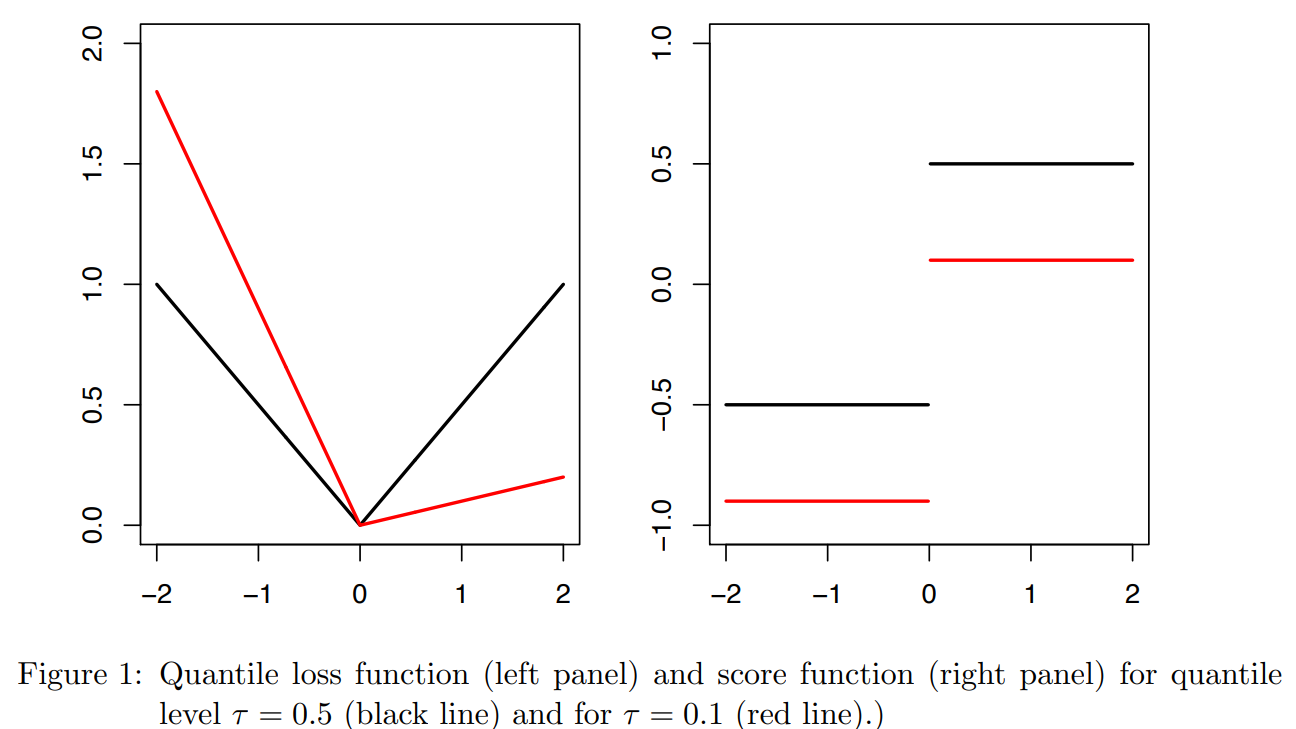
\includegraphics[width=0.58\textwidth]{figures/09-quantile-loss-function.jpg}
  \caption{$\rho_\tau(y)$ 函数的图像，图片来自~\cite{chen2023recursive}。}
  \label{fig:ch9:quantile-loss-function}
\end{figure}

不难证明 $$\operatorname*{\arg\min}_{\theta\in\mathbb R}\mathbb E[\rho_\tau(X-\theta)]=F^{-1}(\tau)$$
从而 $\tau$-样本分位数 $\widehat{\theta}$ 可以表示为 M-估计量：\[M_n(\theta) := \frac{1}{n}\sum_{j=1}^n \rho_\tau(X_j - \theta)\]
对 $\rho_\tau$ 取次导数 (subderivative)，也可以表示为 Z-估计量：\[\Psi_n(\theta) := \frac{1}{n}\sum_{j=1}^n \left((1 - \tau)\mathbb{I}(X_j < \theta) - \tau\mathbb{I}(X_j> \theta)\right) = 0\]
需要说明的是，上述 $\Psi_n(\theta)$ 可能是存在跳跃的，导致 $\Psi_n(\theta)=0$ 无解，如图~\ref{fig:ch9:z-estimator-jump} 所示：

\begin{figure}[htbp]
  \centering
  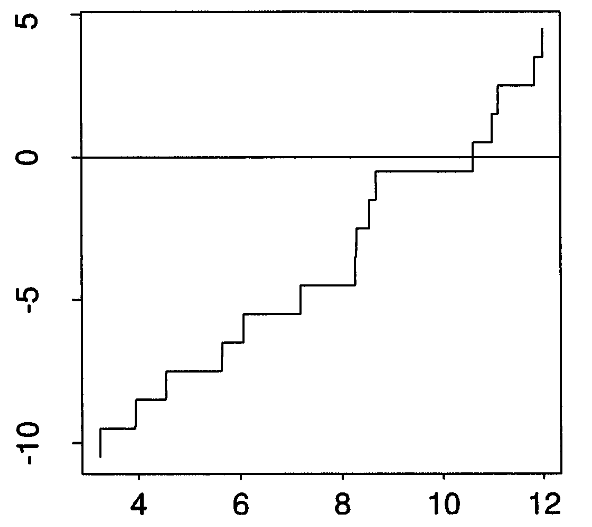
\includegraphics[width=0.58\textwidth]{figures/09-z-estimator-jump.png}
  \caption{从 $\mathrm{Gamma}(5,1)$ 抽取 15 个样本得到的 $\Psi_n(\theta)$。图片来自 \cite{vandervaart1998}, p.~44}
  \label{fig:ch9:z-estimator-jump}
\end{figure}

但也没关系：只要 $n$ 足够大，找一个近似解就已足够。


\end{example}

\begin{example}[Huber 估计量]
Huber 估计量的提出源于鲁棒估计中关于极端数据点对估计影响的研究。众所周知，样本中位数鲁棒但统计效率低、样本均值效率高但对异常值敏感，于是 Huber 估计量试图融合两者的优点。 定义\[\psi(x) = [x]_k := \begin{cases}  -k & \text{若 } x \leq -k \\ x & \text{若 } |x| \leq k \\ k & \text{若 } x \geq k  \end{cases}\]
\textbf{\emph{Huber 估计量}} 求解以下估计方程：
\[
\Psi_n(\theta) = \frac{1}{n}\sum_{j=1}^n \psi(X_j - \theta) = 0.
\]

当数据点距离当前估计值较近（$|X_j- \theta| \leq k$）时，Huber 估计量表现得像均值；当数据点距离较远时，它对异常值的影响进行截断，从而表现得像中位数。参数 $k$ 控制着这个''距离阈值''。

关于 Huber loss 在现代统计学中的应用，感兴趣的读者可以参考 \cite{sunzhoufan2020,hanhuanglinshen2022}。


\end{example}

\section{M 和 Z-估计的相合性}

记参数空间为 $\Theta$ ，配备度量 $d$ ，则相合性指的是 $d(\widehat\theta_n,\theta_0)\overset P\to 0$ ，我们记作 $\widehat\theta_n\overset P\to \theta_0$ 。

\subsection{基本结论}

假设 M-估计 $\widehat\theta_n=\widehat\theta_n(X_1,\dots,X_n)$ 最大化某随机准则函数 $\theta\mapsto M_n(\theta)$ ，即，\[\widehat\theta_n=\operatorname*{\arg\max}M_n(\theta)\]
显然，要想得知 $\widehat\theta_n$ 的渐近行为，必须要考察 $M_n$ 的渐近行为。

首先，我们期望有一个``渐近准则函数'' $\theta\mapsto M(\theta)$ 使得\[M_n(\theta)\overset P\longrightarrow M(\theta),\quad \text{ 当 }n\to\infty,\quad \text{ 对 }\forall \theta\in\Theta\]
当 $M_n(\theta)$ 形如 $\mathbb P_nm_\theta$ 时，可以用大数律直接得出 $M(\theta)=Pm_\theta$ （只要这个期望存在的话）。

真实参数 $\theta_0$ 定义为最大化 $M(\theta)$ 的点：

\[
\theta_0:=\operatorname*{\arg\max}_{\theta\in\Theta}\mathbb E[m_\theta(X)].
\]
非常自然地，我们期望 $M_n$ 的最大值点 $\widehat{\theta}_n$ 能收敛到 $M$ 的最大值点 $\theta_0$。这也是本节首先要证明的东西。不过，要证明这一点，

\begin{itemize}
\tightlist
\item
  $M_n(\theta)\overset P\to M(\theta)$ 的条件有些不太够，至少也要加强到一致收敛，才能保证函数在``形状''上能越来越接近。
\item
  $\theta_0$ 应当是``\textbf{\emph{良分离}} (well separated)''的最大值点。所谓``良分离''是一个比唯一性更强的要求： $M$ 在所有 $d(\theta,\theta_0)\ge\epsilon$ 的点 $\theta$ 处取值都应该能够与 $\theta_0$ 处的值分离开。一个反例如图~\ref{fig:ch9:well-separated} 所示：这个函数有唯一最大值点，但是在无穷远处可能渐近趋近于该最大值，这是我们不愿看到的。
\end{itemize}

\begin{figure}[htbp]
  \centering
  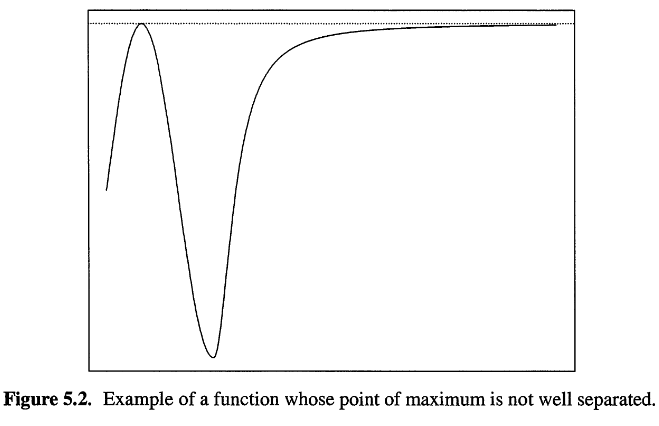
\includegraphics[width=0.68\textwidth]{figures/09-well-separated-maximum.png}
  \caption{唯一但非良分离的最大值点。图片来自 \cite{vandervaart1998}, p.~45}
  \label{fig:ch9:well-separated}
\end{figure}

最后，鉴于找到 $M_n$ 的精确最值可能不容易也不必要，我们只要求找到一个近似的最值作为 $\widehat\theta_n$ ，只需要让 $M_n(\widehat\theta_n)$ 真实最大值的差距是 $o_P(1)$ 的，这称作\textbf{\emph{近似最大条件}} (nearly maximization condition)。

\begin{theorem}[M-估计的相合性]
\label{thm:ch9:m-estimator-consistency}

设 $M_n$ 是随机准则函数而 $M$ 是一个 $\theta$ 的确定函数， $\theta_0=\operatorname*{\arg\max}M(\theta)$ ，假设下面三个条件满足：

\begin{enumerate}
\def\labelenumi{\arabic{enumi}.}
\tightlist
\item
  【一致收敛】 $\sup\limits_{\theta\in\Theta}|M_n(\theta)-M(\theta)|\overset P\to 0$ ；
\item
  【良分离】对每个 $\epsilon>0$ ， $\sup\limits_{\theta\in\Theta,\  d(\theta,\theta_0)\ge\epsilon}M(\theta)<M(\theta_0)$ ；
\item
  【近似最大条件】 $\widehat\theta_n$ 满足 $M_n(\widehat\theta_n)\ge\sup\limits_{\theta\in\Theta}M_n(\theta)-o_P(1)$
\end{enumerate}

那么 $\widehat\theta_n\overset P\longrightarrow \theta_0$ 。

\end{theorem}

\begin{proof}

根据``良分离''条件 (2.)，对任意 $\epsilon>0$，存在 $\eta>0$ 使得
\[
M(\theta)<M(\theta_0)-\eta,\qquad
\forall \theta\in\Theta:\ d(\theta,\theta_0)\ge\epsilon.
\]
若取 $\theta=\widehat\theta_n$，得出 $\big\{d(\widehat\theta,\theta_0)\ge \epsilon\big\}\subset \big\{M(\widehat\theta_n)<M(\theta_0)-\eta\big\}$，即

\begin{equation}
\label{eq:ch9:tag-2}
P\big(d(\widehat\theta_n,\theta_0)\ge\epsilon\big)\le P\big(M(\theta_0)-M(\widehat\theta_n)>\eta\big)
\end{equation}

我们用条件 (3.) 和 (1.) 证明式~\eqref{eq:ch9:tag-2} 右侧收敛于 0：\[ M_n(\widehat\theta_n)\ge\sup\limits_{\theta\in\Theta}M_n(\theta)-o_P(1)\ge M_n(\theta_0)-o_P(1)=M(\theta_0)-o_P(1) \]从而\[M(\theta_0)-M(\widehat\theta_n)\le M_n(\widehat\theta_n)-M(\widehat\theta_n)+o_P(1)\le \sup\limits_{\theta\in\Theta}|M_n(\theta)-M(\theta)|+o_P(1)=o_P(1)\]
于是在式~\eqref{eq:ch9:tag-2} 中取 $n\to\infty$ 即证出 $d(\widehat\theta_n,\theta_0)\overset P\to 0$ 。

\end{proof}

Z-估计的结论和 M-估计如出一辙，只需把定理~\ref{thm:ch9:m-estimator-consistency} 的叙述稍加改动，

\begin{theorem}[Z-估计的相合性]\label{thm:ch9:z-estimator-consistency}

设 $\Psi_n$ 是随机向量值函数， $\Psi$ 是 $\theta$ 的确定向量值函数， $\theta_0$ 满足 $\Psi(\theta_0)=0$ ，假设下面三个条件满足：

\begin{enumerate}
\def\labelenumi{\arabic{enumi}.}
\tightlist
\item
  【一致收敛】 $\sup\limits_{\theta\in\Theta}\|\Psi_n(\theta)-\Psi(\theta)\|\overset P\to 0$ ；
\item
  【良分离】 对每个 $\epsilon>0$ 有 $\inf\limits_{\theta\in\Theta,\ d(\theta,\theta_0)\ge\epsilon}\|\Psi(\theta)\|>0=\|\Psi(\theta_0)\|$ ；
\item
  【近似零条件 (nearly zero condition)】 $\Psi_n(\widehat\theta_n)=o_P(1)$ 。
\end{enumerate}

那么 $\widehat\theta_n\overset P\to \theta_0$ 。

\end{theorem}

\begin{proof}

对 $M_n(\theta)=-\|\Psi_n(\theta)\|$ 和 $M(\theta)=-\|\Psi(\theta)\|$ 用定理~\ref{thm:ch9:m-estimator-consistency}。

\end{proof}

\subsection{更松的相合性条件}

定理~\ref{thm:ch9:m-estimator-consistency} 的良分离可以适当进行修改，得到下述更容易验证的形式：

\begin{theorem}[紧参数空间中的 M-估计相合性]\label{thm:ch9:m-estimator-compact-consistency}

设如下条件成立：

\begin{enumerate}
\def\labelenumi{\arabic{enumi}.}
\tightlist
\item
  【一致收敛】定理~\ref{thm:ch9:m-estimator-consistency} 的条件 (1.)；
\item
  【唯一最大值点】 $M(\theta)=\mathbb E[m_\theta(X)]$ 在 $\theta_0$ 处唯一取得最大值；
\item
  【紧性】参数空间 $\Theta$ 是紧空间；
\item
  【连续性】 $\theta\mapsto M(\theta)$ 连续。
\end{enumerate}

那么，对任意满足

\begin{enumerate}
\def\labelenumi{\arabic{enumi}.}
\setcounter{enumi}{4}
\tightlist
\item
  $M_n(\widehat\theta_n)\ge M_n(\theta_0)-o_P(1)$
\end{enumerate}

的 $\widehat\theta_n$ ，都成立 $\widehat\theta_n\overset P\to \theta_0$ 。

\end{theorem}

\begin{proof}

对任意 $\delta>0$ ，我们记 $B_\delta(\theta_0):=\{\theta:d(\theta,\theta_0)<\delta\}$ 代表 $\theta_0$ 为中心的球。从参数空间中挖去这个球，连续函数 $M$ 在紧集 $\Theta\cap B^c(\theta_0)$ 上有最大值点，记作 $\theta^*$ 。则 (2.) 保证，
$$M(\theta^*)=\sup\limits_{\theta\in\Theta\cap B^c(\theta_0)}M(\theta)<M(\theta_0).$$

下面我们要证明，对任意 $\epsilon>0$ ，当 $n\to\infty$时，下面的式子以趋近于 1 的概率成立

\begin{equation}
\label{eq:ch9:tag-3}
M(\widehat\theta_n)>M_n(\widehat\theta_n)-\frac\epsilon3>M_n(\theta_0)-\frac{2\epsilon}3>M(\theta_0)-\epsilon
\end{equation}

怎么做呢？

\begin{itemize}
\tightlist
\item
  第一个不等号来自于条件 (1.)，一致收敛告诉我们 $P\left(M(\widehat\theta_n)\le M_n(\widehat\theta_n)-\tfrac\epsilon3\right)=o(1)$ ；
\item
  第二个不等号来自于 (5.)，其表明 $P\left(M_n(\widehat\theta_n)\le M_n(\theta_0)-\tfrac\epsilon3\right)=o(1)$ ，或者说， $M_n(\widehat\theta_n)\ge M_n(\theta_0)-o_P(1)>M_n(\theta_0)-\tfrac\epsilon3$ 以趋近于 1 的概率成立；
\item
  第三个不等号与第一个不等号同理。
\end{itemize}

取 $\epsilon=M(\theta_0)-M(\theta^*)>0$ ，代入式~\eqref{eq:ch9:tag-3} 得到：以趋近于 1 的概率\[M(\widehat\theta_n)>M(\theta^*)\]
此时肯定有 $d(\widehat\theta_n,\theta_0)<\delta$ ，因 $M(\theta^*)$ 是 $\Theta\cap B^c(\theta_0)$ 中的最大值；由 \[ 1\leftarrow P\big(M(\widehat\theta_n)>M(\theta^*)\big)\le P\big(d(\widehat\theta_n,\theta_0)<\delta\big)\le 1 \]知 $n\to\infty$ 时， $P\big(d(\widehat\theta_n,\theta_0)<\delta\big)\to 1$ ，从而证明了结论。

\end{proof}

接下来我们把目光放在``一致收敛''这个条件上。一致收敛可以由如下概念进行刻画：

\begin{definition*}[Glivenko--Cantelli 类]
一族可测函数 $\mathscr F$ 若满足 $\|\mathbb P_n-P\|_{\mathscr F}:=\sup\limits_{f\in\mathscr F}|\mathbb P_nf-Pf|\to 0\quad \text{a.s.}$，
则称 $\mathscr F$ （关于 $P$ ）是一个 \textbf{\emph{Glivenko-Cantelli 类}} (Glivenko-Cantelli class)，简称 GC 类。
\end{definition*}

当 $M_n(\theta)=\mathbb P_n m_\theta$ 、 $M(\theta)=Pm_\theta$ 时，`` $M_n(\theta)$ 一致收敛到 $M(\theta)$ ''实际上是在要求 $\{m_\theta:\theta\in\Theta\}$ 构成一个 GC 类；一个充分条件如下：

\begin{proposition}[一致大数律的一个充分条件]
\label{prop:ch9:gc-sufficient-condition}
设 $\Theta$ 是紧度量空间，对每个 $x\in\mathscr X$，函数 $\theta\mapsto m_\theta(x)$ 都是 a.s. 连续的，且这些 $m_\theta(x)$ 都被某可积函数控制，那么 $\{m_\theta:\theta\in\Theta\}$ 是 GC 类。
\end{proposition}

上述结论称作\emph{一致大数律} (ULLN)。

% \href{https://www.zhihu.com/question/387169516/answer/1147878576}{谁可以解释一下``一致大数定律''?}

Z-估计的情况是相同的，设 $\psi_\theta=(\psi_{\theta,1},\dots,\psi_{\theta,k})^\top$ ，那么 $\Psi_n(\theta)=\mathbb P_n\psi_\theta$ 一致收敛到 $\Psi(\theta)=P\psi_\theta$ ，实际上是在要求 $\{\psi_{\theta,i},\theta\in\Theta,i=1,\dots,k\}$ 构成 GC 类。

但是，一致收敛这个条件其实过于强了，并且在实际中很难去验证。如果想更精细地刻画一致收敛，往往需要借助经验过程 (Empirical Process) 的工具，建议读者参考 \cite{vandervaartwellner1996}、\cite{geer2000}。

下面的定理提供了 Z-估计相合、不要求一致收敛的情形，来自 \cite{vandervaart1998} 一书 Lemma 5.10 (p.47)，

\begin{theorem}[单调 Z-估计的相合性]\label{thm:ch9:monotone-z-consistency}

设 $\Theta\subset\mathbb R$ ， $\Psi_n$ 是随机函数， $\Psi$ 是 $\theta$ 的确定函数， $\Psi_n(\theta)\overset P\to\Psi(\theta)$ 对每个 $\theta\in\Theta$ 成立（逐点收敛），设有如下条件，

\begin{enumerate}
\def\labelenumi{\arabic{enumi}.}
\tightlist
\item
  如下条件其中之一成立：
\end{enumerate}

\begin{itemize}
\tightlist
\item
  对每个 $\theta\in\Theta$ ，函数 $\theta\mapsto \Psi_n(\theta)$ 连续，并且有唯一的零点 $\widehat\theta_n$ ；
\item
  对每个 $\theta\in\Theta$ ，函数 $\theta\mapsto \Psi_n(\theta)$单调非降，且 $\Psi_n(\widehat\theta_n)=o_P(1)$ ；
\end{itemize}

\begin{enumerate}
\def\labelenumi{\arabic{enumi}.}
\setcounter{enumi}{1}
\tightlist
\item
  $\theta_0$ 满足：对任意 $\epsilon>0$ ， $\Psi(\theta_0-\epsilon)<0<\Psi(\theta_0+\epsilon)$ 。
\end{enumerate}

那么 $\widehat\theta_n\overset P\to \theta_0$ 。

\end{theorem}

\begin{proof}

如果 $\theta\mapsto \Psi_n(\theta)$ 连续且有唯一的零点 $\widehat\theta_n$ ，那么事件 $\{\Psi_n(\theta_0-\epsilon)<0<\Psi_n(\theta_0+\epsilon)\}$ 蕴含 $\theta_0-\epsilon<\widehat\theta_n<\theta_0+\epsilon$ ，即， 
$$P\Big(\Psi_n(\theta_0-\epsilon)<0<\Psi_n(\theta_0+\epsilon)\Big)\le P\big(\theta_0-\epsilon<\widehat\theta_n<\theta_0+\epsilon\big)$$
上式左侧是收敛于 1 的，因为 $\Psi_n(\theta_0\pm\epsilon)\overset P\to\Psi(\theta_0\pm\epsilon)$ ，从而上式右侧也收敛于 1，这证明了 $\widehat\theta_n\overset P\to\theta_0$ 。

下面证明 $\theta\mapsto \Psi_n(\theta)$ 单调非降的情形。对每个 $\eta>0$ ，当 $\Psi_n(\theta_0-\epsilon)<-\eta$ 成立时，由单调性，若 $\widehat\theta_n\le\theta_0-\epsilon$ ，则 
$\Psi_n(\widehat\theta_n)\le\Psi_n(\theta_0-\epsilon)<-\eta$ ，即 
$$\{\Psi_n(\theta_0-\epsilon)<-\eta\}\cap \{\widehat\theta_n\le\theta_0-\epsilon\}\subset \{\Psi_n(\widehat\theta_n)<-\eta\}$$

从而 $$P(\Psi_n(\theta_0-\epsilon)<-\eta)\le P(\widehat\theta_n>\theta_0-\epsilon)+\underbrace{P(\Psi_n(\widehat\theta_n)<-\eta)}_{o(1)}$$

另一个方向同理，于是对每个 $\epsilon,\eta>0$ ，\[\begin{aligned} P\big(\Psi_n(\theta_0-\epsilon)<-\eta,\Psi_n(\theta_0+\epsilon)>\eta\big) \le P\big(\theta_0-\epsilon<\widehat\theta_n<\theta_0+\epsilon\big)+o(1) \end{aligned}\]
取 $2\eta=\min\{-\Psi(\theta_0-\epsilon),\Psi(\theta_0+\epsilon)\}$ 则上式左侧收敛于 1。

\end{proof}

\begin{example}[样本中位数的相合性]\label{ex:ch9:median-consistency}
设 $\mathbb R$ 上的随机变量 $X\sim F$ ，其中 $F$ 有唯一的总体中位数 $\theta_0$ ，这里的``唯一''是指对任意 $\epsilon>0$ ，
\[
P(X<\theta_0-\epsilon)<0.5<P(X<\theta_0+\epsilon).
\]
样本中位数 $\widehat\theta_n$ 作为 Z-估计可以写作下述方程的解：
\[
\Psi_n(\theta)=\frac1n\sum_{j=1}^n\mathrm{sign}(X_j-\theta).
\]

根据大数律，对每个 $\theta$ ， 
$$\Psi_n(\theta)\overset P\to \Psi(\theta)=\mathbb{E}[\mathrm{sign}(X-\theta)]=P(X>\theta)-P(X<\theta)$$
容易验证：

\begin{itemize}
\tightlist
\item
  $\theta\mapsto-\Psi_n(\theta)$ 单调非降；
\item
  $-\Psi(\theta_0-\epsilon)<0<-\Psi(\theta_0+\epsilon)$ 。
\end{itemize}
那么根据定理~\ref{thm:ch9:monotone-z-consistency}， $\widehat\theta_n\overset P\to \theta_0$ 。

\end{example}

类似于前面的中位数例子，请读者结合分位数估计的例子和定理~\ref{thm:ch9:monotone-z-consistency} 自行证明：如果 $F$ 有唯一的 $\tau$ 分位数 $F^{-1}(\tau)$ ，则样本 $\tau$ -分位数 $\mathbb F_n^{-1}(\tau)$ 也是相合估计。


\subsection{Wald 的相合性证明}

本节中我们介绍另一组条件，来自 Wald 在 1949 年对 MLE 的相合性证明，这里既不需要一致收敛，也放宽了连续性、紧性，从而提供了一个更一般的框架。

首先引入一个比连续性更弱的概念：\emph{\textbf{\href{https://en.wikipedia.org/wiki/Semi-continuity}{半连续性}} }。

\begin{definition*}[半连续性]
实值函数 $f$ 如果满足\[\limsup_{x \to x_0} f(x) \leq f(x_0)\]
则称其在点 $x_0$ 处\textbf{\emph{上半连续}} （upper semi-continuous, u.s.c.）；如果\[\liminf_{x \to x_0} f(x) \geq f(x_0)\]
则称其在点 $x_0$ 处\textbf{\emph{下半连续}} （lower semi-continuous, l.s.c.）。
\end{definition*}

图~\ref{fig:ch9:semicontinuity} 直观展示了上半连续与下半连续的区别\footnote{注意，上/下半连续与左/右连续没有任何关系。}。

\begin{figure}[htbp]
  \centering
  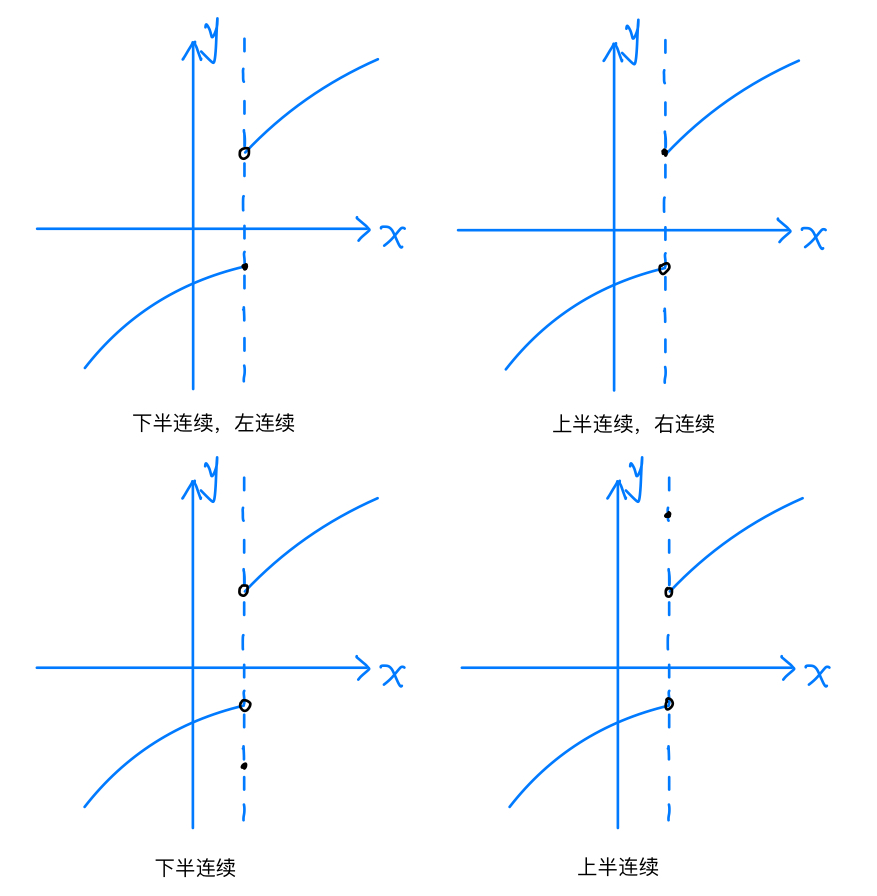
\includegraphics[width=0.62\textwidth]{figures/09-semicontinuity.png}
  \caption{上半连续与下半连续的示意图。图片来自 \url{https://www.cnblogs.com/BoyaYan/p/17237330.html}}
  \label{fig:ch9:semicontinuity}
\end{figure}

% （注意，上/下半连续与左/右连续没有任何关系。）%，例子见 \url{https://math.stackexchange.com/q/3884576}。）

对函数 $\theta\mapsto Pm_\theta=\mathbb{E}_P[m_\theta(X)]$ ，之前的假设都是它有唯一的最大值点 $\theta_0$ 。但在这里，我们允许它有多个最大值点，并记 \[ \Theta_0:=\big\{\theta_0\in\Theta:Pm_{\theta_0}=\sup\nolimits_\theta Pm_\theta\big\}\ne\varnothing \]代表所有能取到最大值的点集。

\begin{theorem}[Wald 相合性]\label{thm:ch9:wald-consistency}

设如下三个条件满足，

\begin{enumerate}
\def\labelenumi{\arabic{enumi}.}
\tightlist
\item
  【u.s.c.】 对每个 $\theta\in\Theta$ ， $\theta\mapsto m_\theta(x)$ a.s. 是上半连续的，即 $\limsup\limits_{\theta_n\to\theta}m_{\theta_n}(x)\le m_\theta(x),\quad \text{a.s.}$ (这里``a.s.''的例外集允许依赖于 $\theta$ 。)
\item
  【局部一致可积】 对每个球 $U\subset\Theta$ ，函数 $x\mapsto \sup\limits_{\theta\in U}m_\theta(x)$ 可测，且满足
  \[
  P\sup_{\theta\in U}m_\theta(x)=\mathbb E_P\left[\sup_{\theta\in U}m_\theta(X)\right]<\infty.
  \]
\item
  【近似最大条件】存在某个 $\theta_0\in\Theta_0$ 使得 $M_n(\widehat\theta_n)\ge M_n(\theta_0)-o_P(1)$ 。
\end{enumerate}

那么，对任意 $\epsilon>0$ 和紧集 $K\subset\Theta$ ，
\[
P(d(\widehat\theta_n,\Theta_0)\ge\epsilon,\ \widehat\theta_n\in K)\to 0.
\]

即， $\widehat\theta_n$ 落在紧集 $K$ 内但与 $\Theta_0$ 内每个点的距离都不低于 $\epsilon$ 的概率趋于 0。

\end{theorem}

\begin{proof}

记集合 $B := \{\theta \in K : d(\theta, \Theta_0) \geq \varepsilon\}$，我们要证明 $P(\widehat{\theta}_n \in B) \to 0$。

首先，如果函数 $\theta \mapsto Pm_\theta$ 恒等于 $-\infty$ ，则 $\Theta_0 = \Theta$，结论平凡成立。否则，我们可以假设存在 $\theta_0\in\Theta_0$ 使得 $Pm_{\theta_0} > -\infty$ ；那么由条件 (2.)， $\mathbb{E}_P[|m_{\theta_0}(X)|]<\infty$ 。

固定某个 $\theta \in K$，令 $U_l \downarrow \theta$ 为围绕 $\theta$ 的直径趋于零的递减开球列。记 $m_U(x) := \sup_{\theta\in U} m_\theta(x)$ ，则对每个 $l$， $m_{U_l}(x)$ 关于 $l$ 递减，且 $m_\theta(x) \leq m_{U_l}(x),\quad \forall\, l$

取 $l\to\infty$ ，

\begin{itemize}
\tightlist
\item
  一方面 $m_\theta(x)\le \lim\limits_{l\to\infty}m_{U_l}(x)$ ；
\item
  令一方面 $U_l$ 收缩到 $\theta$ ，再结合 $m_\theta(x)$ 的上半连续性 (1.)， $\lim\limits_{l\to\infty} m_{U_l}(x) \leq m_\theta(x)$ a.s.。
\end{itemize}

从而 $\lim\limits_{l\to\infty} m_{U_l}(x) = m_\theta(x)$ ，即 $m_{U_l} \downarrow m_\theta$ a.s.。
对函数列 $\{-m_{U_l}\}$ 用单调收敛定理，有 \footnote{这里的右侧可能是 $-\infty$ 。}

$$\mathbb{E}[m_{U_l}(X)] \to \mathbb{E}[m_\theta(X)] ,\quad \text{ 当 }l\to\infty$$


当 $\theta\not\in\Theta_0$ 时，由于 $\mathbb{E}[m_{U_l}(X)] \to \mathbb E[m_\theta(X)]<\mathbb E[m_{\theta_0}(X)]$ ，故在序列 $\{U_l\}$ 中总存在一个包含 $\theta$ 的开球 $U_\theta$ 使得

\begin{equation}
\label{eq:ch9:tag-4}
\mathbb E[m_{U_\theta}(X)]<\mathbb E[m_{\theta_0}(X)]
\end{equation}

注意到$\{U_\theta : \theta \in B\}$ 构成 $B$ 的一个开覆盖，由于 $K$ 是紧集，其闭子集 $B \subset K$ 也是紧集，故存在有限子覆盖 $U_{\theta_1}, \dots, U_{\theta_p}$。由大数律 ，

\begin{equation}
\label{eq:ch9:tag-5}
\begin{aligned} \sup_{\theta\in B}\mathbb P_nm_\theta&\le\max_{i=1,\dots,p}\sup_{\theta\in U_{\theta_i}} \mathbb P_nm_\theta\\ &\le \max_{i=1,\dots,p}\mathbb P_n\sup_{\theta\in U_{\theta_i}}m_\theta\\ &\xrightarrow{\text{a.s.}}\max_{i=1,\dots,p}\mathbb{E}\left[\sup_{\theta\in U_{\theta_i}}m_\theta(X)\right]\\ &<\mathbb{E}[m_{\theta_0}(X)] \end{aligned}
\end{equation}

其中最后一行来自式~\eqref{eq:ch9:tag-4} 。

另一方面，如果 $\widehat\theta_n\in B$ ，那么根据条件 (3.) 和大数律\[ \sup_{\theta \in B} \mathbb{P}_n m_\theta \geq \mathbb{P}_n m_{\widehat{\theta}_n} \geq \mathbb{P}_n m_{\theta_0} - o_P(1) = \mathbb{E}[m_{\theta_0}(X)]-o_P(1) \]

这表明事件 $\{\widehat{\theta}_n \in B\}$ 蕴含 $\sup\limits_{\theta\in B} \mathbb{P}_n m_\theta \ge \mathbb{E}[m_{\theta_0}(X)] - o_P(1)$。结合式~\eqref{eq:ch9:tag-5} ，\[P(\widehat\theta_n\in B)\le P\left(\sup_{\theta\in B}\mathbb P_nm_\theta\ge\mathbb E[m_{\theta_0}(X)]-o_P(1)\right)\to 0\]
\end{proof}

\begin{remark}

\begin{itemize}
\tightlist
\item
  为了应用此定理，参数空间 $\Theta$ 最好是紧的；不然的话，应当额外表明 $\widehat\theta_n$ 最终会落入某个紧集，或者对参数空间进行合适的紧化 (compactification)。
\item
  一种方法是对 $m_\theta$ 施加强制条件 (Coercivity condition)，即当 $|\theta|\to\infty$ 时 $m_\theta\to -\infty$ ，从而 $\widehat\theta_n$ 总是胎紧的，其概率集中在某个紧集内。
\item
  虽然 $\mathbb R$ 在通常拓扑下不是紧空间，但是我们可以加入两个点 $\overline{\mathbb R}:=\mathbb R\cup\{-\infty,\infty\}$ 构成扩展实数轴。 $\arctan$ 是 $\overline{\mathbb R}$ 到闭区间 $\left[-\tfrac\pi2,\tfrac\pi2\right]$ 的一个同胚，从而 $\overline{\mathbb R}$ 就是一个紧度量空间，其度量可取 $d(x,y)=|\arctan x-\arctan y|$ 。
\end{itemize}
\end{remark}

\begin{example}[Cauchy 似然]
Cauchy 分布 $\text{Cauchy}(\theta)$ 的 PDF 为
\[
p_\theta(x)=\frac1{\pi(1+(x-\theta)^2)},\quad x\in\mathbb R.
\]
其中 $\theta$ 是位置参数，我们取参数空间为扩展实数轴 $\Theta=\overline{\mathbb R}$ 。

设有 i.i.d. 样本 $X_1,\dots,X_n$ ，则 $\theta$ 的 MLE 最大化 $\theta\mapsto\mathbb P_nm_\theta$ ，其中， 
$$m_\theta(x)=-\log(1+(x-\theta)^2)$$
特别地，定义\[\begin{aligned} m_{-\infty}(x)&=\limsup_{\theta\to-\infty}m_\theta(x)=-\infty\\ m_{\infty}(x)&=\limsup_{\theta\to\infty}m_\theta(x)=-\infty\\  \end{aligned}\]
我们验证一下定理~\ref{thm:ch9:wald-consistency} 的条件：

\begin{enumerate}
\def\labelenumi{\arabic{enumi}.}
\tightlist
\item
  首先 $m_\theta(x)$ 是连续的，自然上半连续；
\item
  局部一致可积：对 $U\subset \Theta$ ，
  \[
  \mathbb E\left[\sup_{\theta\in U}m_\theta(X)\right]=\int_{\mathbb R}\sup_{\theta\in U}\frac{-\log(1+(x-\theta)^2)}{\pi(1+(x-\theta)^2)}{\rm d}x<\infty.
  \]
\item
  $\widehat\theta_n$ 是 MLE，自然满足 $M_n(\widehat\theta_n)=\sup\limits_{\theta\in\Theta}M_n(\theta)\ge M_n(\theta_0)-o_P(1)$ 。
\end{enumerate}
由可识别性， $\Theta_0=\{\theta_0\}$ ，故定理~\ref{thm:ch9:wald-consistency} 给出 $\widehat\theta_n\overset P\to \theta_0$ 。


\end{example}

\section{M 和 Z-估计的渐近正态性}

\subsection{经验过程与 Donsker 类}

要证明渐近正态性，我们不得不引入一些经验过程的工具。如果读者不想看这些东西，大可以跳过本节，只需承认本节末尾的式~\eqref{eq:ch9:tag-6} 成立就可以。

设 $X_1,\dots,X_n$ 是来自分布 $P$ 的 i.i.d. 样本， $\mathbb P_n=\frac1n\sum_{j=1}^n\delta_{X_j}$ 是经验测度。定义\href{https://en.wikipedia.org/wiki/Empirical_process}{经验过程} (Empirical process)\[\mathbb G_n:=\sqrt n(\mathbb P_n-P)\]
我们可以将 $\mathbb G_n$ 看作是一个符号测度，用于衡量经验分布与真实分布的差距。对可积函数 $f:\mathscr X\to\mathbb R$ ，定义经验过程在 $f$ 处的取值为 
$$\mathbb G_nf=\sqrt n(\mathbb P_nf-Pf)=\sqrt n\left(\frac1n\sum_{j=1}^n\ f(X_j)-\mathbb E[f(X)]\right)$$s
给定一族 $\mathscr X\to \mathbb R$ 的 $P$ -可积函数 $\mathscr F$ ，则上述 $P$ 、 $\mathbb P_n$ 和 $\mathbb G_n$ 又都可以视作 $\mathscr F\to \mathbb R$ 的算子。

记 $\ell^\infty(\mathscr F)$ 是所有 $\mathscr F\to \mathbb R$ 的有界算子构成的 Banach 空间：
\[
x\in \ell^\infty(\mathscr F)\quad \iff \quad \sup_{f\in\mathscr F}|x(f)|<\infty.
\]
如果函数族 $\mathscr F$ 满足
\[
\sup_{f\in\mathscr F}|f(x)-Pf|<\infty,\qquad \forall x\in\mathscr X,
\]
那么 $\mathbb G_n$ 还可以视作从 $\ell^\infty (\mathscr F)$ 中取值的随机元。
$$\mathbb G_n:\omega\mapsto \sqrt n\left(\frac1n\sum_{j=1}^nf(X_j(\omega))-\mathbb{E}[f(X)]\right)$$
我们考察其在 $\ell^\infty(\mathscr F)$ 中的极限：
\begin{definition*}[Donsker 类]
若存在 $\ell^\infty(\mathscr F)$ 中 Borel-可测的、胎紧的随机元 $\mathbb G_P$，使得 $\mathbb G_n$ 在 $\ell^\infty(\mathscr F)$ 中弱收敛到 $\mathbb G_P$，那么称 $\mathscr F$ 是一个 \textbf{\emph{Donsker 类}}，或者 $P$-Donsker 类。
\end{definition*}

当每个 $f$ 平方可积（即 $Pf^2<\infty$ ）时，由经典中心极限定理， $\mathbb G_n f\overset{\rm d}\to \mathcal N(0,\mathrm{Var}[f(X)])$ ；Donsker 类就建立在这种观察上，它的定义本质上是在说``使得这种弱收敛成立的那些函数族''。

我们对比一下 GC-类和 Donsker 类，

\begin{itemize}
\tightlist
\item
  Glivenko-Cantelli (GC) 类对应的是一致的大数律，它保证了经验均值 $\mathbb{P}_n f$ 在整个函数族上都一阶收敛到真实期望 $Pf$。
\item
  Donsker 类对应的是一致的中心极限定理，它保证经验过程 $\mathbb G_n$ 在 $\ell^\infty(\mathscr F)$ 中整体弱收敛到一个极限随机元 $\mathbb G_P$ 。
\end{itemize}

这个极限元 $\mathbb G_P$ 是一个零均值 \textbf{\emph{Gaussian 过程}} ，这指的是，对每个 $k=1,2,\dots<\infty$ 和任意 $f_1,\dots ,f_k\in\mathscr F$ ， 
$$(\mathbb G_P f_1,\mathbb G_P f_2,\dots,\mathbb G_Pf_k)\sim \mathcal N_k(\mathbf{0},\Sigma)$$
其中 $\Sigma$ 是 $k\times k$ 矩阵，其 $i,j$ 元为 $P(f_i-P f_i)(f_j-Pf_j)=\mathrm{Cov}_{X\sim P}[f_i(X),f_j(X)]$ 。

\begin{example}[Brownian 桥]
记分布函数 $F(t)=P(X\le t)$ 和经验分布函数 $\mathbb F_n(t)=\mathbb P_n(X\le t)$，$\mathscr F=\{\mathbb I(\cdot \le t)\}_{t\in\mathbb R}$。
\end{example}

\begin{theorem}[Donsker--Skorokhod--Kolmogorov 定理]
\label{thm:ch9:donsker}
函数类 $\mathscr F$ 是 Donsker 类，且 $\mathbb G_n(t)=\sqrt n(\mathbb F_n(t)-F(t))\overset{\rm d}\to \mathbb G_P(t)$。
\end{theorem}

其中 $\mathbb G_P(t)$称作 $P$ -\textbf{\emph{Brownian 桥}} ，这是一个 Gaussian 过程，且由于对 $s,t\in\mathbb R$ 有 $\mathbb E[\mathbb I(X\le s)\mathbb I(X\le t)]=F(s\wedge t)$ ，故
\[
\mathrm{Cov}[\mathbb G_P(t),\mathbb G_P(s)]=F(s\wedge t)-F(s)F(t).
\]

\begin{remark}

\begin{itemize}
\tightlist
\item
  上例中的弱收敛可以视作是在 $\ell^\infty(\overline{\mathbb R})$ 中的收敛，也可以视作是在其子空间： \href{https://en.wikipedia.org/wiki/Skorokhod_space}{Skorokhod 空间} $\mathcal D(-\infty,\infty)$ 中的收敛。当配备上确界范数 $\|\cdot\|_\infty$ 时，选择哪个空间并不影响结论。
\item
  最早是由 Donsker 于 1952 年对 $[0,1]$ 上的均匀分布证明了这一结论，一个证明可以参考 \cite{linluzhang2023} 一书的 §8.3。
\end{itemize}
\end{remark}

\begin{example}[Lipschitz 函数类]\label{ex:ch9:lipschitz-function}
设 $\Theta\subset\mathbb R^d$ 紧， $\mathscr F=\{f(x,\theta)\}_{\theta\in\Theta}$ ，其中 $f:\mathscr X\times \Theta\to\mathbb R$ 。设对每个 $x$ ， $f(x,\cdot)$ 是 $L(x)$ -Lipschitz 的，即 $|f(x,\theta_1)-f(x,\theta_2)|\le L(x)\|\theta_1-\theta_2\|$

如果 $L(x)$ 是平方可积的，那么可以证明 $\mathscr F$ 是 Donsker 类： 
$$\mathbb G_n(\theta)=\sqrt n(\mathbb P_nf(\theta,\cdot)-Pf(\theta,\cdot))\overset{\rm d}\to \mathbb G(\theta)$$
其中 
$$\mathrm{Cov}(\mathbb G(\theta_0),\mathbb G(\theta_1))=\mathrm{Cov}_{X\sim P}[f(X,\theta_0),f(X,\theta_1)]$$


\end{example}
这两个例子也可参考 \cite{duchi2018stats300b15}。

下面证明一个非常有用的引理，来自 \cite{vandervaart1998} 的 Lemma 19.24。它说的是：如果我们用 $\mathscr F$ 中的一列函数 $\widehat f\!_n$ 去逼近某个 $f_0$ ，那么经验过程作用在 $\widehat f\!_n$ 上和作用在 $f_0$ 上的效果相同。这相当于``用相合估计量替换参数不会改变渐近分布''。


\begin{lemma}[Donsker 类中的随机替换]\label{lem:ch9:donsker-random-substitution}

设 $\mathscr{F}$ 是一族可测函数的 $P$ -Donsker 类， $\{\widehat{f}\!_n\}$ 为一列在 $\mathscr{F}$ 中取值的随机元，使得对某个 $f_0\in L^2(P)$ （即 $Pf_0^2<\infty$ ）有
\[
\int_{\mathscr X} (\widehat{f}_n(x) - f_0(x))^2 \,\mathrm{d}P(x) = P(\widehat{f}\!_n - f_0)^2 \overset{P}{\to} 0.
\]

则 $\mathbb G_n(\widehat f\!_n-f)\overset P\to 0$ ，从而， $\mathbb G_n\widehat f\!_n\overset{\rm d}\to \mathbb G_P f_0$ 。

\end{lemma}

\begin{proof}

不失一般性，可以假设 $f_0\in\mathscr F$ ，否则用 $\mathscr F\cup\{f_0\}$ 替换 $\mathscr F$ 仍然保持 Donsker 类。考虑
\[
g:\ell^\infty(\mathscr F)\times\mathscr F\to\mathbb R,\quad g(z,f)=z(f)-z(f_0).
\]

为 $\mathscr F$ 赋予 $L_2(P)$ 度量，那么只要 $f\mapsto z(f)$ 在 $f$ 处连续， $g$ 在 $(z,f)$ 就在乘积空间中是连续的。这是因为：若在 $\ell^\infty(\mathscr F)\times\mathscr F$ 中 $(z_n,f_n)\to (z,f)$ ，则 $z_n$ 一致收敛到 $z$ ，故若 $z$ 在 $f$ 处连续时
\[
z(f_n)=z(f)+o(1)\longrightarrow z(f).
\]
由引理中的条件， $\widehat f\!_n$ 在 $L_2(P)$ 下收敛到 $f_0$ ，这蕴含了在 $(\mathscr F,L_2(P))$ 中的依概率收敛 $\widehat f\!_n\overset P\to f_0$ 。又由于 $\mathscr F$ 是 $P$ -Donsker 类，在 $\ell^\infty(\mathscr F)$ 中有 $\mathbb G_n\overset{\rm d}\to \mathbb G_P$ 。二者结合，在 $\ell^\infty(\mathscr F)\times \mathscr F$ 中，
\[
(\mathbb G_n,\widehat f\!_n)\overset{\rm d}\to (\mathbb G_P,f_0).
\]

Gaussian 过程 $\mathbb G_P$ 的轨道在 $\mathscr F$ 上几乎处处连续， 从而， $g$ 在几乎每个点 $(\mathbb G_P,f_0)$ 处连续。由连续映射定理，
\[
\mathbb G_n\big(\widehat f\!_n-f_0\big)=g(\mathbb G_n,\widehat f\!_n)\overset{\rm d}\to g(\mathbb G_P,f_0)=0.
\]

\end{proof}

设 $\widehat{f}\!_n := \psi_{\widehat{\theta}_n}$，$f_0 := \psi_{\theta_0}$，且存在平方可积的 $\dot{\psi}$ 使得，\[P(\psi_{\widehat{\theta}_n} - \psi_{\theta_0})^2 \leq P(\dot{\psi}^2) \|\widehat{\theta}_n - \theta_0\|^2 = O_P(\|\widehat{\theta}_n - \theta_0\|^2)\]
如果 $\widehat{\theta}_n \overset{P}{\to} \theta_0$，则上式趋于 0。因此，只要函数类 $\{\psi_\theta\}$ 是 $P$ -Donsker 的，根据引理~\ref{lem:ch9:donsker-random-substitution}，我们就有\[\mathbb{G}_n(\psi_{\widehat{\theta}_n} - \psi_{\theta_0}) \overset{P}{\to} 0\]
即

\begin{equation}
\label{eq:ch9:tag-6}
\sqrt{n}(\mathbb{P}_n \psi_{\widehat{\theta}_n} - P\psi_{\widehat{\theta}_n}) = \sqrt{n}(\mathbb{P}_n \psi_{\theta_0} - P\psi_{\theta_0}) + o_P(1)
\end{equation}

这一结论在后面的渐近正态证明中有重要作用。

\subsection{渐近正态性的证明}

首先证明 Z-估计的结论，我们先简单描述一下思路和动机。从估计方程出发：Z-估计满足 $\Psi_n(\widehat{\theta}_n)=\mathbb P_n\psi_{\widehat\theta_n}=0$ ，而参数真值满足 $\Psi(\theta_0)=P\psi_{\theta_0}=0$ 。在 $\theta_0$ 处将 $\Psi$Taylor 展开，\[\Psi(\widehat\theta_n)\approx \Psi(\theta_0)+\Psi'(\theta_0)(\widehat\theta_n-\theta_0)\]
由于 $\Psi(\theta_0)=0$，这给出了 $\widehat\theta_n-\theta_0$ 与 $\Psi(\widehat\theta_n)$ 的近似线性关系： $\sqrt n(\widehat\theta_n-\theta)\approx (\Psi'(\theta_0))^{-1}\Psi(\widehat\theta_n)$ 。 但这里面的 $\Psi(\widehat\theta_n)$ 是未知的！我们需要用经验过程把它替换掉：注意到 \[ \Psi(\widehat\theta_n) = \Psi(\widehat\theta_n) - \Psi_n(\widehat\theta_n) = (P-\mathbb P_n)\psi_{\widehat\theta_n} \]从而 $\sqrt{n}(\widehat\theta_n-\theta_0) \approx (\Psi'(\theta_0))^{-1} \sqrt{n}(P-\mathbb P_n)\psi_{\widehat\theta_n}$；利用式~\eqref{eq:ch9:tag-6} ，把右侧的 $\psi_{\widehat\theta_n}$ 替换为 $\psi_{\theta_0}$ ，那么根据经典中心极限定理，上式右侧是收敛于总体分布的： 
$$\sqrt{n}(P -\mathbb P_n)\psi_{\theta_0} \;\overset{\rm d}{\to}\; N\bigl(0,\, P\psi_{\theta_0}\psi_{\theta_0}^\top\bigr)$$ 
一言以蔽之，利用 Taylor 展开将估计方程转化为经验过程的线性形式，并通过式~\eqref{eq:ch9:tag-6} 将 $\widehat\theta_n$ 替换为真值 $\theta_0$ ，从而将估计量的极限分布归结为经验过程的中心极限定理。

下面是严格一些的论述，

\begin{theorem}[Z-估计的渐近正态性]\label{thm:ch9:z-estimator-asymptotic-normality}

假设：

\begin{enumerate}
\def\labelenumi{\arabic{enumi}.}
\tightlist
\item
  对欧氏空间某开子集中的每个 $\theta$，设 $x \mapsto \psi_\theta(x)$ 为可测向量值函数；
\item
  对 $\theta_0$ 某邻域内的每对 $\theta_1$ 和 $\theta_2$，存在一维可测函数 $\dot{\psi}(x)$ 满足 $P\dot{\psi}^2 < \infty$，使得
  \[
  \|\psi_{\theta_1}(x) - \psi_{\theta_2}(x)\| \leq \dot{\psi}(x)\|\theta_1 - \theta_2\|.
  \]
\item
  $P\|\psi_{\theta_0}\|^2 < \infty$，且映射 $\theta \mapsto P\psi_\theta$ 在 $\theta_0$ 处可微，有非奇异 Jacobian 矩阵
  \[
  V_{\theta_0} := \frac{\partial}{\partial\theta} P\psi_\theta \Big|_{\theta=\theta_0}.
  \]
\item
  $\widehat\theta_n$ 满足 $\mathbb{P}_n \psi_{\widehat{\theta}_n} = o_P(n^{-1/2})$ 且 $\widehat{\theta}_n \overset{P}{\to} \theta_0$。
\end{enumerate}

则\[\sqrt{n}(\widehat{\theta}_n - \theta_0) = -V_{\theta_0}^{-1} \frac{1}{\sqrt{n}}\sum_{j=1}^n \psi_{\theta_0}(X_j) + o_P(1) \ \overset{\mathrm{d}}{\to}\ \mathcal{N}\left(0,\ V_{\theta_0}^{-1} P\psi_{\theta_0}\psi_{\theta_0}^\top(V_{\theta_0}^{-1})^\top\right)\]
\end{theorem}

\begin{proof}

首先，条件 (2.) 和例~\ref{ex:ch9:lipschitz-function} 表明 $\{\psi_\theta\}$ 构成 Donsker 类，则前文式~\eqref{eq:ch9:tag-6} 成立。注意到 $P\psi_{\theta_0}=0$ ，且条件 (4.) 给出 $\sqrt{n}\mathbb{P}_n\psi_{\widehat{\theta}_n} = o_P(1)$ ，再结合式~\eqref{eq:ch9:tag-6} 得到，

\begin{equation}
\label{eq:ch9:tag-7}
\begin{aligned} \sqrt{n}(P\psi_{\theta_0} - P\psi_{\widehat{\theta}_n}) &= -\sqrt{n}P\psi_{\widehat{\theta}_n} \\ &= \underbrace{\sqrt{n}(\mathbb{P}_n\psi_{\widehat{\theta}_n} - P\psi_{\widehat{\theta}_n})}_{\sqrt{n}(\mathbb{P}_n\psi_{\theta_0} - P\psi_{\theta_0}) + o_P(1)} - \underbrace{\sqrt{n}\mathbb{P}_n\psi_{\widehat{\theta}_n} }_{o_P(1)}\\  &= \sqrt n\mathbb P_n\psi_{\theta_0} + o_P(1)  \end{aligned}
\end{equation}

现在对 式~\eqref{eq:ch9:tag-7}左侧在 $\theta_0$ 处做 Taylor 展开 ，由条件 (3.)，\[\begin{aligned} \sqrt n(P\psi_{\widehat\theta_n} -  P\psi_{\theta_0}) &= \sqrt nV_{\theta_0}(\widehat\theta_n-\theta_0) + \sqrt no(\|\widehat\theta_n-\theta_0\|)\\  \end{aligned}\]
代入式~\eqref{eq:ch9:tag-7} ：
\begin{equation}
\label{eq:ch9:tag-8}
\sqrt{n}V_{\theta_0}(\widehat{\theta}_n - \theta_0) =\underbrace{-\sqrt n\mathbb P_n \psi_{\theta_0}}_{O_P(1)} + o_P(1)+o(\sqrt{n}\|\widehat{\theta}_n - \theta_0\|)
\end{equation}

现在要证明 $\sqrt{n}\|\widehat{\theta}_n - \theta_0\| = O_P(1)$ ，从而上式里的 $o(\sqrt n\|\widehat\theta_n-\theta\|)=o_P(1)$ ；这也是容易的，因为式~\eqref{eq:ch9:tag-8} 同时告诉我们
\[
\sqrt{n}\|\widehat{\theta}_n - \theta_0\| \le \|V_{\theta_0}^{-1}\|\sqrt n\|V_{\theta_0}(\widehat{\theta}_n - \theta_0)\|=O_P(1)+o(\sqrt{n}\|\widehat{\theta}_n - \theta_0\|).
\]
从而由 Slutsky 定理，式~\eqref{eq:ch9:tag-8} 的后两项可以忽略，我们便证明了
\[
\sqrt{n}V_{\theta_0}(\widehat{\theta}_n - \theta_0) = -\frac{1}{\sqrt{n}}\sum_{j=1}^n \psi_{\theta_0}(X_j) + o_P(1).
\]

渐近正态性由经典中心极限定理即可。

\end{proof}

M-估计的结论完全类似，只需将定理~\ref{thm:ch9:z-estimator-asymptotic-normality} 的 $\psi_\theta$ 改成 $m_\theta$ 对 $\theta$ 的导数，我们这里也写作定理，

\begin{theorem}[M-估计的渐近正态性]\label{thm:ch9:m-estimator-asymptotic-normality}

假设：

\begin{enumerate}
\def\labelenumi{\arabic{enumi}.}
\tightlist
\item
  对欧氏空间某开子集中的每个 $\theta$， $x \mapsto m_\theta(x)$ 为可测函数，使得 $\theta \mapsto m_\theta(x)$ 在 $\theta_0$ 处对 $P$-几乎所有 $x$ 可微，导数记作 $\dot{m}_{\theta_0}(x)$。
\item
  对 $\theta_0$ 邻域内的每对 $\theta_1$ 和 $\theta_2$，存在可测函数 $\dot{m}(x)$ 满足 $P\dot{m} ^2 < \infty$，使得
  \[
  |m_{\theta_1}(x) - m_{\theta_2}(x)| \leq \dot{m}(x)\|\theta_1 - \theta_2\|.
  \]
\item
  $\theta \mapsto Pm_\theta$ 在最大值点 $\theta_0$ 处有二阶 Taylor 展开
  \[
  Pm_\theta = Pm_{\theta_0} + \frac{1}{2}(\theta-\theta_0)^\top V_{\theta_0} (\theta-\theta_0) + o(\|\theta-\theta_0\|^2),
  \]
  有非奇异对称 Hessian 矩阵
  \[
  V_{\theta_0} = \frac{\partial^2}{\partial\theta^2} Pm_\theta \big|_{\theta=\theta_0}.
  \]
\item
  $\widehat\theta_n$ 满足 $\mathbb{P}_n m_{\widehat{\theta}_n} \geq \sup_\theta \mathbb{P}_n m_\theta - o_P(n^{-1})$ 且 $\widehat{\theta}_n \overset{P}{\to} \theta_0$。
\end{enumerate}

则\[\sqrt{n}(\widehat{\theta}_n - \theta_0) = -V_{\theta_0}^{-1} \frac{1}{\sqrt{n}}\sum_{j=1}^n \dot{m}_{\theta_0}(X_j) + o_P(1) \ \overset{\mathrm{d}}{\to}\ \mathcal{N}\left(0,\ V_{\theta_0}^{-1} P\dot{m}_{\theta_0}\dot{m}_{\theta_0}^\top V_{\theta_0}^{-1}\right).\]


\end{theorem}
还有值得一提的是，在经典的 M-估计渐近正态证明中，类似于第~\ref{ch:maximum-likelihood}~章的定理~\ref{thm:ch7:mle-asymptotic-normality}，往往要求准则函数存在三阶导数、且三阶导数可被控制。显然，这个条件过于严格，但相应证明更简单，不需要经验过程的工具，并且适用于不少例子，如下。


\begin{theorem*}[Z-估计渐近正态性的另一表述]

若对每个 $x$，$\theta\mapsto\psi_\theta(x)$ 二次连续可微，且 $\Psi(\theta_0)=P\psi_{\theta_0}=0$，$P\|\psi_{\theta_0}\|^2<\infty$，矩阵 $V:=P\dot{\psi}_{\theta_0}$ 非奇异，且其所有二阶偏导在 $\theta_0$ 的某邻域内被一个可积函数 $\dot{\psi}(x)$ 控制，则对任意满足 $\Psi_n(\widehat{\theta}_n)=\mathbb P_n\psi_{\widehat\theta_n}=0$ 的相合估计量 $\widehat{\theta}_n$，有\[\sqrt{n}(\widehat{\theta}_n-\theta_0) = -(P\dot{\psi}_{\theta_0})^{-1}\frac{1}{\sqrt{n}}\sum_{j=1}^n\psi_{\theta_0}(X_j) + o_P(1)\]
\end{theorem*}

\begin{proof}

由 Taylor 展开，\[0=\Psi_n(\widehat{\theta}_n)=\Psi_n(\theta_0)+\dot{\Psi}_n(\theta_0)(\widehat{\theta}_n-\theta_0)+\frac12(\widehat{\theta}_n-\theta_0)^\top\ddot{\Psi}_n(\widetilde{\theta}_n)(\widehat{\theta}_n-\theta_0)\]
其中 $\dot\Psi_n(\theta):=\mathbb P_n\dot\psi_{\theta}$ 、 $\ddot{\Psi}_n(\theta)=\mathbb P_n\ddot{\psi}_\theta$ 。中心极限定理给出 $\sqrt{n}\Psi_n(\theta_0)\overset{\rm d}\to \mathcal{N}(0,P\psi_{\theta_0}\psi_{\theta_0}^\top)$、大数律给出 $\dot{\Psi}_n(\theta_0)\overset{P}{\to} V=P\dot{\psi}_{\theta_0}$，余项由一致可积控制为 $O_P(\|\widehat{\theta}_n-\theta_0\|^2)$；再结合相合性保证 $\|\widehat{\theta}_n-\theta_0\|=o_P(1)$，故余项为 $o_P(\|\widehat{\theta}_n-\theta_0\|)$。整理后得
\[
-\Psi_n(\theta_0)=(V+o_P(1))(\widehat\theta_n-\theta_0).
\]
注意到 $V+o_P(1)$ 以趋于 1 的概率可逆，两边左乘 $\sqrt{n}$ 并乘以 $(V+o_P(1))^{-1}$ 即得结论。

\end{proof}

类似于第~\ref{ch:maximum-likelihood}~章的定理~\ref{thm:ch7:score-root-consistency}，当 $n\to \infty$ 时，可以证明这里的 $\Psi_n(\widehat{\theta}_n)=0$ 也以趋于 1 的概率至少有一个解，并且存在一列解满足 $\widehat\theta_n\overset P\to \theta_0$。

\subsection{例子}

\begin{example}[样本中位数的渐近正态性]\label{ex:ch9:median-asymptotic}
样本中位数作为 M-估计可以视作最大化准则函数 $\theta\mapsto -\sum_{j=1}^n|X_j-\theta|$ 。记 $\theta_0=F^{-1}(0.5)$ 是总体中位数，且分布函数 $F$ 在 $\theta_0$ 处可微，有严格正的密度 $f(\theta_0)$ 。为了应用后面的 M-估计渐近正态性定理，考虑
\[
m_\theta(x)=|x-\theta|-|x|.
\]
它对 $\theta$ 是 1-Lipschitz 的：
\[
|m_{\theta_1}(x)-m_{\theta_2}(x)|\leq|\theta_1-\theta_2|,
\]
且 $\dot{m}_\theta\equiv 1$。

计算 $Pm_\theta$：\[\begin{aligned} Pm_\theta &= \int_{\mathbb R} |x-\theta| \,\mathrm{d}F(x) - \int_{\mathbb R} |x| \,\mathrm{d}F(x) \\ &=\theta F(0)+\int_0^\theta2(\theta-x)\mathrm{d}F(x)-\theta(1-F(0))\\ &= 2\int_0^\theta F(x)\,\mathrm{d}x - \theta  \end{aligned}\]
最后一步来自分部积分。可见 $Pm_\theta$ 在 $\theta_0$ 处确实是二次可微的：其导数为 $2F(\theta_0)-1$，二阶导数为 $2f(\theta_0)$。于是渐近方差为
\[
V_{\theta_0}^{-1} P\dot{m}_{\theta_0}^2 V_{\theta_0}^{-1} = \frac{1}{(2f(\theta_0))^2}.
\]

根据定理~\ref{thm:ch9:m-estimator-asymptotic-normality}，
\[
\sqrt{n}(\widehat{\theta}_n - \theta_0) \overset{\mathrm{d}}{\to} \mathcal{N}\left(0, \frac{1}{(2f(\theta_0))^2}\right).
\]

\end{example}


请读者结合例~\ref{ex:ch9:quantile} 自行验证：如果把这里的中位数改成 $\tau$ -分位数 $F^{-1}(\tau)$ 、样本中位数改成 $\mathbb F_n^{-1}(\tau)$ ，则相应的结论如下\footnote{见 \cite{vandervaart1998} 的 Problem 5.11。更一般的关于样本分位数的渐近正态性质，以及 Bahadur 表示等结论，可参考包括但不限于~\cite{chenxiru2009} 的 §4.4.2。}：
\[\sqrt{n}(\mathbb F_n^{-1}(\tau) - F^{-1}(\tau)) \overset{\mathrm{d}}{\to} \mathcal{N}\left(0, \frac{\tau(1-\tau)}{(f(\theta_0))^2}\right)\]
% \href{https://www.zhihu.com/question/1579360351}{一般抽样的均值为正态分布，那抽样的其他统计特征如中位数、百分位数等会是什么分布呢？}


\begin{example}[非线性最小二乘]\label{ex:ch9:nonlinear-least-squares}
考虑回归模型 $Y = f_{\theta_0}(X) + \varepsilon$，其中 $f_\theta$ 是一参数族回归函数，余项 $\varepsilon$ 满足 \[ \mathbb{E}[\varepsilon|X]=0,\quad \mathrm{Var}[\varepsilon|X]=\sigma^2(X)<\infty \]给定独立样本 $(X_1,Y_1),\dots,(X_n,Y_n)$ ，\emph{最小二乘估计量} (LSE) 的目标是最小化 $\sum_{j=1}^n (Y_j - f_\theta(X_j))^2$，对应 M-估计量 $m_\theta(x,y) = (y-f_\theta(x))^2$------方便起见，我们这里把 M-估计量的``最大化''改成``最小化''。

\begin{equation}
\label{eq:ch9:tag-9}
\begin{aligned} P m_\theta &= \mathbb{E}\bigl[(Y-f_\theta(X))^2\bigr] \\ &= \mathbb{E}\bigl[(Y-f_{\theta_0}(X) + f_{\theta_0}(X)-f_\theta(X))^2\bigr] \\ &= \mathbb{E}\bigl[\varepsilon^2\bigr] + \mathbb{E}\bigl[(f_{\theta_0}(X)-f_\theta(X))^2\bigr] \end{aligned}
\end{equation}
因此，最小化 $P m_\theta$ 等价于最小化 $\mathbb{E}[(f_{\theta_0}(X)-f_\theta(X))^2]$。若模型可识别，则 $\theta_0$ 是唯一最大值点。

假设存在可测函数 $\dot{f}(x)$ 使得\[|f_{\theta_1}(x) - f_{\theta_2}(x)| \le \dot{f}(x)\,\|\theta_1-\theta_2\|\]
且存在 $c(x)$ 使得 $|f_\theta(x)|\le c(x)$ 对所有 $\theta$ 成立，则\[\begin{aligned} |m_{\theta_1}(x,y)-m_{\theta_2}(x,y)| &= \bigl|(y-f_{\theta_1})^2-(y-f_{\theta_2})^2\bigr| \\ &= |f_{\theta_1}-f_{\theta_2}| \cdot|2y-f_{\theta_1}-f_{\theta_2}| \\ &\le \dot{f}(x)\,\|\theta_1-\theta_2\|\,\bigl(2|y|+2c(x)\bigr) \end{aligned}\]
令 $\dot{m}(x,y) = \dot{f}(x)\bigl(2|y|+2c(x)\bigr)$，再设：

\begin{itemize}
\tightlist
\item
  设 $\dot f$ 和 $c$ 的性质足够好使得 $\dot m$ 平方可积，从而定理~\ref{thm:ch9:m-estimator-asymptotic-normality} 的 Lipschitz 条件 (2.) 成立。
\item
  设 $f_\theta(x)$ 在 $\theta_0$ 处连续可微， $V_{\theta_0}=\left.\frac{\mathrm{d}^2}{\mathrm{d}\theta^2}Pm_{\theta}\right|_{\theta=\theta_0}$ 正定，从而定理~\ref{thm:ch9:m-estimator-asymptotic-normality} 的 (3.) 成立。
\end{itemize}

我们来算一下 $V_{\theta_0}$ ， 由式~\eqref{eq:ch9:tag-9} ，\[\begin{aligned} P m_\theta &= \mathbb{E}[\varepsilon^2]+\mathbb{E}[(f_{\theta_0}(X)-f_\theta(X))^2]\\ &=P m_{\theta_0} + \int_{\mathscr X} \bigl(f_\theta(x)-f_{\theta_0}(x)\bigr)^2 \,\mathrm{d}P_X(x)\\  \end{aligned}\]
将 $f_\theta(x)-f_{\theta_0}(x) = (\theta-\theta_0)^\top\dot{f}\!_{\theta_0}(x) + o(\|\theta-\theta_0\|)$ 代入，得\[P m_\theta = P m_{\theta_0} + \frac{1}{2}(\theta-\theta_0)^\top V_{\theta_0}(\theta-\theta_0) + o(\|\theta-\theta_0\|^2)\]
其中
\[
V_{\theta_0} = 2\int \dot{f}\!_{\theta_0}(x)\dot{f}\!_{\theta_0}(x)^\top\,\mathrm{d}P_X(x) = 2P\dot{f}\!_{\theta_0}\dot{f}\!_{\theta_0}^{\ \top}.
\]

设有 i.i.d. 观测 $(X_1,Y_1),\dots,(X_n,Y_n)$ 以及真实误差项 $\varepsilon_j=Y_j-f_{\theta_0}(X_j)$ ；取相合估计 $\widehat\theta_n$ 满足定理~\ref{thm:ch9:m-estimator-asymptotic-normality} 的条件 (4.)，则 M-估计量的渐近正态性给出\[\begin{aligned} \sqrt{n}(\widehat{\theta}_n-\theta_0) &= -V_{\theta_0}^{-1}\,\frac{1}{\sqrt{n}}\sum_{j=1}^n \dot{m}_{\theta_0}(X_j,Y_j) + o_P(1)\\ &=V_{\theta_0}^{-1}\,\frac{2}{\sqrt{n}}\sum_{j=1}^n \varepsilon_j\dot{f}\!_{\theta_0}(X_j) + o_P(1)\\ &\overset{\rm d}\to\mathcal N\Big(0,\bigl(P\dot{f}_{\theta_0}\dot{f}_{\theta_0}^\top\bigr)^{-1} \mathbb{E}\left[\varepsilon^2\dot{f}_{\theta_0}\dot{f}_{\theta_0}^\top\right] \bigl(P\dot{f}_{\theta_0}\dot{f}_{\theta_0}^\top\bigr)^{-1}\Big) \end{aligned}\]
若 $\varepsilon$ 与 $X$ 独立且 $\mathbb{E}[\varepsilon^2]=\sigma^2$，则上面的渐近方差为 $\sigma^2 \bigl(P\dot{f}_{\theta_0}\dot{f}_{\theta_0}^\top\bigr)^{-1}$ 。


\end{example}

\begin{example}[二分类回归]\label{ex:ch9:binary-classification}
设 $(X_j,Y_j),\ j=1,\dots,n$ 独立，其中协变量 $X_j$ 是 $k$ 维的随机向量，响应变量是 0-1 随机变量： $Y_j\in\{0,1\}$。设 $P_\theta(Y_j=1|X_j=x)=\Psi(\theta^\top x)$，其中 $\Psi:\mathbb R\to[0,1]$ 是已知的、连续可微的、严格单调递增的分布函数，如 logistic 函数 $\frac1{1+e^{-t}}$ （对应 logistic 回归），或者标准正态分布函数（对应 probit 模型）。

MLE 最大化条件似然\[\begin{aligned} L_n(\theta) &= \prod_{j=1}^n \Psi(\theta^\top X_j)^{Y_j} \bigl(1 - \Psi(\theta^\top X_j)\bigr)^{1 - Y_j}\\ \ell_n(\theta)&=\log L_n(\theta)=\sum_{j=1}^nY_j\log\Psi(\theta^\top X_j)+(1-Y_j)\log(1-\Psi(\theta^\top X_j)) \end{aligned}\]
对应的准则函数为
\[
m_\theta(x,y)=y\log\Psi(\theta^\top x)
+(1-y)\log(1-\Psi(\theta^\top x)).
\]
对 $\theta$ 求导得到\[\psi_\theta(x,y)=\left(\frac{y}{\Psi(\theta^\top x)}-\frac{1-y}{1-\Psi(\theta^\top x)}\right)\Psi'(\theta^\top x)\,x=\frac{y-\Psi(\theta^\top x)}{\Psi(\theta^\top x)(1-\Psi(\theta^\top x))}\Psi'(\theta^\top x)\,x\]
易见，如果限制在紧集上， $\psi_{\theta}(x,y)$ 对每个 $x,y,\theta$ 一致有界，且总对 $\theta$ 连续。再作一些假设，

\begin{itemize}
\tightlist
\item
  为了确保参数 $\theta$ 的可识别性，设协变量 $X_j$ 的分布不集中在 $\mathbb{R}^k$ 的任何一个 $(k-1)$ 维仿射子空间上。
\item
  简单起见，设 $X$ 有界且矩阵 $\mathbb{E}[XX^\top]$ 非奇异。
\end{itemize}
此时可以验证定理~\ref{thm:ch9:m-estimator-consistency} 的条件，从而 MLE $\widehat\theta_n$ 是相合估计。

记 Fisher 信息矩阵为\[I(\theta) = \mathbb{E}\left[\frac{\Psi'(\theta^\top X)^2}{\Psi(\theta^\top X)(1-\Psi(\theta^\top X))}XX^\top\right]\]
于是定理~\ref{thm:ch9:z-estimator-asymptotic-normality} 给出\[\sqrt{n}(\widehat{\theta}_n - \theta) \overset{\mathrm{d}}{\to} \mathcal{N}(0, I^{-1}(\theta))\]
\end{example}
\section{讨厌参数与两步估计}

在实际问题中，感兴趣的参数往往与\emph{讨厌参数} (nuisance parameter) 共存。例如，

\begin{itemize}
\tightlist
\item
  对于正态分布 $\mathcal N(\mu,\sigma^2)$ ，其中 $\mu\in\mathbb R$ 、 $\sigma^2<\infty$ 均未知，我们可能只希望估计均值 $\mu$ ，然而未知的方差 $\sigma^2$ 也会影响均值的估计。
\item
  在例~\ref{ex:ch9:median-asymptotic} 中，可以为协变量 $x=x_\eta$ 增加参数化的假设，于是当估计 $\theta$ 本身时， $\eta$ 就是一个讨厌参数。
\item
  在带有缺失数据的回归中，我们想估计某回归系数 $\theta$，但缺失概率函数 $\omega_\eta(x)$ 是未知的。后面例~\ref{ex:ch9:nonlinear-least-squares} 我们会具体介绍这个例子。
\end{itemize}

一般地，设 $X_1,\dots,X_n$ i.i.d.，分布函数为 $F_{\theta,\eta}$ ，其中 $\theta$ 是感兴趣的参数、 $\eta$ 是讨厌参数；此时无论是 M-估计的 $m_\theta$ 还是 Z-估计的 $\psi_\theta$ 都既依赖于 $\theta$ 又依赖于 $\eta$ 。我们往往不得不先找出 $\eta$ 的一个估计，记作 $\widehat\eta_n$ ，然后再将之``插入 (plug-in)''到 $\theta$ 的估计方程里，如
\[
P_n\psi_{\theta,\widehat\eta_n}=\frac1n\sum_{j=1}^n\psi_{\theta,\widehat\eta_n}(X_j)=0.
\]

从而解得 $\widehat\theta_n$ ------本质上是一个\emph{两步法} (2-step procedure)。此时的渐近性质又如何呢？

\subsection{缺失响应回归}

\begin{example}[缺失响应回归]
考虑回归模型 $Y_j = m_{\theta_0}(X_j) + \varepsilon_j$，$\mathbb{E}[\varepsilon_j|X_j]=0$。响应变量 $Y_j$ 可能缺失，记\[ R_j := \begin{cases} 1, & \text{若 } Y_j \text{ 被观测到}\\ 0, & \text{若 } Y_j \text{ 缺失} \end{cases} \]
作\emph{随机缺失}（Missing at Random, MAR）假设：
\[
P(R_i=1| X_j,Y_j) = P(R_j=1| X_j) = \omega_{\eta_0}(X_j).
\]

它说的是： $Y_j$ 缺失与否仅依赖于 $X_j$ ，和 $Y_j$ 自己没有关系，即缺失机制完全由观测到的协变量解释。 $\omega_{\eta_0}(\cdot)$ 称作缺失倾向函数（missing propensity function），其形式已知，本例中就是一个简单的二分类模型， $\eta_0$ 是其中的参数------可以是一个有限维参数，甚至也可以是非参数的设置。

最简单的方法是，在 MAR 假设下，未观测到的那些数据都是可以忽略掉的，我们只拿观测到的数据进行回归。LSE 最小化 $\sum_{j=1}^n R_j \bigl(Y_j - m_\theta(X_j)\bigr)^2$ ，求导得其估计方程为

\begin{equation}
\label{eq:ch9:tag-10}
\sum_{j=1}^n R_j \bigl(Y_j - m_\theta(X_j)\bigr) \frac{\partial m_\theta}{\partial\theta}(X_j) = 0
\end{equation}

在真值 $\theta_0$ 处，利用 MAR 假设和 $\mathbb{E}[\epsilon_j | X_j] = 0$，有\[\mathbb{E}\left[ R_j \bigl(Y_j - m_{\theta_0}(X_j)\bigr) \frac{\partial m_{\theta_0}}{\partial\theta}(X_j) \right] = \mathbb{E}\left[ \frac{\partial m_{\theta_0}}{\partial\theta}(X_j) \,\omega_{\eta_0}(X_j) \,\mathbb{E}[\varepsilon_j | X_j] \right] = 0\]
因此，由估计方程~\eqref{eq:ch9:tag-10} 解出的 $\widehat\theta_n$ 估计量是无偏的，从而在一定正则条件下，它可以是相合估计，且具有渐近正态性。

第二种方法称作\emph{逆概率加权}（Inverse Probability Weighting, IPW）。其思想是：用缺失倾向函数 $\omega_{\eta_0}$ 的倒数对残差进行加权，以校正缺失带来的偏差：

\begin{equation}
\label{eq:ch9:tag-11}
\sum_{j=1}^n \frac{R_j}{\omega_{\eta_0}(X_j)} \bigl(Y_j - m_\theta(X_j)\bigr) \frac{\partial m_\theta}{\partial\theta}(X_j) = 0
\end{equation}

这里的加权不会改变期望：MAR 假设下 $\mathbb{E}[R_j \varepsilon_j | X_j] = \omega_{\eta_0}(X_j) \mathbb{E}[\varepsilon_j |X_j] = 0$，从而\[\mathbb{E}\left[ \frac{R_j}{\omega_{\eta_0}(X_j)} \varepsilon_j \frac{\partial m_{\theta_0}}{\partial\theta}(X_j) \right] = \mathbb{E}\left[ \frac{\partial m_{\theta_0}}{\partial\theta}(X_j) \frac{1}{\omega_{\eta_0}(X_j)} \,\mathbb{E}[R_j \varepsilon_j | X_j] \right]=0.\]
因此，如果 $\eta_0$ 已知的话，由式~\eqref{eq:ch9:tag-11} 解出的 $\widehat\theta_n$ 也是无偏的。

然而， $\eta_0$ 是未知的。用例~\ref{ex:ch9:nonlinear-least-squares}中完全一样的二分类方法，求解 
$$\sum_{j=1}^n \left( \frac{R_j}{\omega_\eta(X_j)} - \frac{1-R_j}{1-\omega_\eta(X_j)} \right) \frac{\partial \omega_\eta(X_j)}{\partial \eta} = 0$$
得到 $\widehat\eta_n$ ，并用它代替式~\eqref{eq:ch9:tag-11} 的 $\eta_0$ 即可。

\end{example}

\begin{remark}
一个比较神奇的结果是，用估计的 $\widehat\eta_n$ 代替 $\eta_0$ 的甚至比已知 $\eta_0$ 时的效率更高！请参考 \cite{chenleungqin2008}。这说明估计讨厌参数未必是一件坏事。
\end{remark}

有时候，`` $\omega_{\eta_0}(x)$ 是参数模型''的假设往往过于强的，也可以考虑非参数的模型 \[ P(R_j=1|X_j,Y_j)=P(R_j=1|X_j)=\omega(X_j) \]我们可以拿非参数的估计方法，例如核密度估计 (KDE) ：\[\widehat\omega_n(x)=\frac{\sum_{j=1}^nK\left(\frac{x-X_j}{h}\right)R_j}{\sum_{j=1}^nK\left(\frac{x-X_j}{h}\right)}\]
其中 $K(\cdot)$ 是某个核函数， $h$ 是平滑带宽 (smoothing bandwidth)，满足当 $n\to \infty$ 时 $h\to 0$ 、 $nh\to \infty$ 。上式的期望实际上就是各 $\omega(X_j)$ 的加权平均：\[\mathbb{E}\bigl[\widehat{\omega}_h(x) |\ X_1,\dots,X_n\bigr] = \frac{\sum_{j=1}^n K\!\left(\frac{x-X_j}{h}\right) \mathbb{E}[R_j | X_j]}{\sum_{j=1}^n K\!\left(\frac{x-X_j}{h}\right)} = \frac{\sum_{j=1}^n K\!\left(\frac{x-X_j}{h}\right) \omega(X_j)}{\sum_{j=1}^n K\!\left(\frac{x-X_j}{h}\right)}\]
当 $x\in\mathbb R^d$ 时，可取 $h\propto n^{-\frac{1}{d+4}}$ ，此时可以证明 (在一定正则条件下) KDE 满足渐近正态性：
\[
\sqrt{nh^d}\big(\widehat\omega_h(x)-\mathbb{E}[\widehat\omega_h(x)]\big)\to \mathcal N(\mu(x),\sigma^2(x)).
\]


\subsection{带讨厌参数时的渐近正态性}

设 $X_1,\dots,X_n$ 独立同分布于 $P$，其分布中有感兴趣的参数 $\theta$ 以及讨厌参数 $\eta$ ，并设我们有一个 $\eta$ 的相合估计 $\widehat\eta_n$ ，我们看看此时由 Z-估计确定的 $\widehat\theta_n$ 是否还能保持定理~\ref{thm:ch9:z-estimator-asymptotic-normality} 的渐近性质。

下面的定理不再作证明（见 \cite{vandervaart1998} 的 Theorem 19.26），我们只关注其结论即可。

\begin{theorem}[带讨厌参数时 Z-估计的渐近正态性]\label{thm:ch9:z-estimator-with-nuisance}

设 $\Theta$ 是 $\mathbb R^k$ 中的开子集， $\eta$ 来自某度量空间，其度量记作 $d$ ， $x\mapsto \psi_{\theta,\eta}(x)$ 是可测向量值函数。设如下条件成立：

\begin{enumerate}
\def\labelenumi{\arabic{enumi}.}
\tightlist
\item
  存在 $\delta>0$ 使得函数类\[ \mathscr{F} = \bigl\{ \psi_{\theta,\eta} : \|\theta-\theta_0\|<\delta,\ d(\eta,\eta_0)<\delta \bigr\} \]是 $P$ -Donsker 类。
\item
  当 $(\theta,\eta)\to(\theta_0,\eta_0)$ 时， $P\bigl\| \psi_{\theta,\eta} - \psi_{\theta_0,\eta_0} \bigr\|^2 \to 0$
\item
  $P\psi_{\theta_0,\eta_0}=0$ 。
\item
  映射 $\theta \mapsto P\psi_{\theta,\eta}$ 在 $\theta_0$ 处可微，且导数 $V_{\theta_0,\eta} := \frac{\partial}{\partial\theta} P\psi_{\theta,\eta}\big|_{\theta=\theta_0}$ 在 $\eta_0$ 的某个邻域内关于 $\eta$ 一致连续，且 $V_{\theta_0,\eta_0}$ 非奇异。
\item
  估计 $\widehat\theta_n,\widehat\eta_n$ 满足 $(\widehat{\theta}_n,\widehat{\eta}_n) \overset{P}{\to} (\theta_0,\eta_0)$ ，且 $\sqrt{n}\,\mathbb{P}_n\psi_{\widehat{\theta}_n,\widehat{\eta}_n} = o_P(1)$。
\end{enumerate}

那么\[\sqrt{n}(\widehat{\theta}_n - \theta_0) = -V_{\theta_0,\eta_0}^{-1}\; \sqrt{n}\, P\psi_{\theta_0,\widehat{\eta}_n} - V_{\theta_0,\eta_0}^{-1}\; \mathbb{G}_n \psi_{\theta_0,\eta_0} + o_P\!\bigl(1 + \sqrt{n}\,\|P\psi_{\theta_0,\widehat{\eta}_n}\|\bigr).\]
\end{theorem}

\begin{remark}

\begin{itemize}
\tightlist
\item
  结论的第一项 $-V_{\theta_0,\eta_0}^{-1} \sqrt{n} P\psi_{\theta_0,\widehat{\eta}_n}$ 刻画了用 $\widehat\eta_n$ 估计讨厌参数 $\eta$ 带来的影响，我们称作漂移项 (drift term)。但多出来这一项并不一定意味着渐近方差一定会增大（如例~\ref{ex:ch9:binary-classification}）。
\item
  如果 $\eta$ 是有限维参数，且 $\eta \mapsto P\psi_{\theta_0,\eta}$ 在 $\eta_0$ 处可微，则我们可以写出 。\[ \sqrt{n}\,P\psi_{\theta_0,\widehat{\eta}_n} = \sqrt{n}\, \frac{\partial P\psi_{\theta_0,\eta_0}}{\partial\eta} (\widehat{\eta}_n-\eta_0) + o_P(1 + \sqrt{n}\|\widehat{\eta}_n-\eta_0\|) \]就算 $\widehat\eta_n-\eta_0$ 本身收敛不够快，但只要方向导数 $\frac{\partial P\psi_{\theta_0,\eta_0}}{\partial\eta}$ 为 0 ，或者足够小（这被称作渐近正交），这也可以帮助我们去除讨厌参数的影响。此时，讨厌参数在真实值附近的小扰动不会引起 $P\psi_{\theta_0,\eta}$ 的过大变化。关于在收敛较慢的讨厌参数下利用 Neyman 正交消除其影响的技术，可参考 \cite{chernozhukov2018}。
\end{itemize}
\end{remark}

\begin{example}[对称位置模型]
设 $X_1, X_2, \dots, X_n$ i.i.d.，其分布函数 $F$ 关于某 $\theta_0$ 对称，即 $F(\theta_0 + x) = 1 - F(\theta_0 - x)$ 对所有 $x$ 成立，我们希望估计位置参数 $\theta_0$ 。

考虑一个 Z-估计量，其估计方程形如\[\frac{1}{n} \sum_{j=1}^n \psi\!\left( \frac{X_j - \theta}{\widehat{\sigma}_n} \right) = 0,\]
其中 $\psi$ 是奇函数（ $\psi(-t) = -\psi(t)$），而 $\widehat{\sigma}_n$ 是某个尺度参数 $\sigma_0$ 的相合估计。$\widehat{\sigma}_n$ 是讨厌参数，不是我们直接关心的。注意到由 $F$ 的对称性和 $\psi$ 是奇函数， \[ P\psi_{\theta_0,\widehat\sigma}=\int_{\mathscr X}\psi\left(\frac{x-\theta_0}{\widehat\sigma}\right)\mathrm{d}F(x)=0,\quad \forall \widehat\sigma \]所以，若定理~\ref{thm:ch9:z-estimator-with-nuisance} 的条件满足，那么它结论中的漂移项是消失的，我们直接得出\[\sqrt{n}(\widehat{\theta}_n - \theta_0) = -V_{\theta_0,\eta_0}^{-1}\,\mathbb{G}_n \psi_{\theta_0,\eta_0} + o_P(1)\]

\end{example}

\section{单步估计}

最后要介绍的主题是所谓的\textbf{\emph{单步估计}} (One-step estimator)，这在第~\ref{ch:maximum-likelihood}~章中已简要提到。

其出发点是，直接求解 M-估计的最大化问题、或者 Z-估计方程可能很困难，本节以 Z-估计为例，遇到的问题可能包括

\begin{itemize}
\tightlist
\item
  估计方程可能有多个解；
\item
  为了保证找到的解足够好（相合性），往往需要对估计方程在整个参数集 $\Theta$ 上有很好的性质。
\end{itemize}

我们知道，\href{https://en.wikipedia.org/wiki/Newton\%27s_method}{Newton-Raphson 算法}是经典的寻找零点的迭代算法。单步估计的方法是：从一个初步的估计 $\widetilde\theta_n$ （往往选择鲁棒估计）出发，然后对估计方程 $\Psi_n(\theta)=0$ ，用 Newton-Raphson 算法进行一步迭代，得到改进的估计量 $\widehat\theta_n$ 。这种估计量得来更简单，同时一步迭代可以 ``纠正'' 初始估计的效率损失，使之和精确求解的 Z-估计有相同的渐近效率。

具体来说，在初始估计 $\widetilde{\theta}_n$ 处做一阶 Taylor 展开：\[\Psi_n(\widetilde{\theta}_n) + \dot{\Psi}_n(\widetilde{\theta}_n)(\theta - \widetilde{\theta}_n) \approx 0\]
解得\[\widehat{\theta}_n = \widetilde{\theta}_n - \dot{\Psi}_n^{-1}(\widetilde{\theta}_n) \Psi_n(\widetilde{\theta}_n)\]
作为单步估计。为了保证单步估计量 $\widehat\theta_n$ 的渐近正态性，我们要求初始估计 $\widetilde\theta_n$ 具备 $\sqrt n$-相合性，但并不要求其本身在渐近意义上是有效的。同时，还有一个很常见的做法是，我们用某个相合估计 $\dot{\Psi}_{n,0}$ 代替上式中的 $\dot{\Psi}_n(\widetilde{\theta}_n)$ 项。最终的结论如下，

\begin{theorem}[单步 Z-估计的渐近性质]\label{thm:ch9:one-step-z-estimator}

设 $\sqrt{n}\Psi_n(\theta_0) \overset{\mathrm{d}}{\to} Z$ 收敛于正态分布，且存在非奇异矩阵 $\dot{\Psi}_0$ 使得对任意常数 $M$，

\begin{equation}
\label{eq:ch9:tag-12}
\sup_{\sqrt{n}\|\theta - \theta_0\| < M} \left\| \sqrt{n}(\Psi_n(\theta) - \Psi_n(\theta_0)) - \dot{\Psi}_0 \sqrt{n}(\theta - \theta_0) \right\| \overset{P}{\to} 0
\end{equation}

设 $\widetilde{\theta}_n$ 是真实参数 $\theta_0$ 的 $\sqrt{n}$-相合的初始估计， $\dot{\Psi}_{n,0}\overset{P}{\to}\dot{\Psi}_0$ ，那么，单步估计量

\begin{equation}
\label{eq:ch9:tag-13}
\widehat{\theta}_n = \widetilde{\theta}_n - \dot{\Psi}_{n,0}^{-1} \Psi_n(\widetilde{\theta}_n)
\end{equation}

满足
\[
\sqrt{n}(\widehat{\theta}_n - \theta_0) = -\dot{\Psi}_0^{-1} \sqrt{n}\Psi_n(\theta_0) + o_P(1)\overset{\rm d}\to -\dot\Psi_0^{-1}Z.
\]

\end{theorem}

\begin{proof}

由式~\eqref{eq:ch9:tag-13} ，

\begin{equation}
\label{eq:ch9:tag-14}
\begin{aligned}\dot{\Psi}_{n,0} \sqrt{n}(\widehat{\theta}_n - \theta_0) &= \dot{\Psi}_{n,0} \sqrt{n}(\widetilde{\theta}_n - \theta_0) - \sqrt{n}\Psi_n(\widetilde{\theta}_n)\\ &=\dot{\Psi}_{n,0} \sqrt{n}(\widetilde{\theta}_n - \theta_0)- \sqrt{n}\Psi_n(\theta_0) - \sqrt{n}\left(\Psi_n(\widetilde{\theta}_n) - \Psi_n(\theta_0)\right) \end{aligned}
\end{equation}

鉴于初始估计满足 $\sqrt n(\widetilde\theta_n-\theta_0)=O_P(1)$ ，对任意 $\epsilon>0$ ，我们可以取 $M$ 充分大使得 $P(\sqrt{n}\|\widetilde{\theta}_n-\theta_0\|<M)>1-\epsilon$ 。从而，由式~\eqref{eq:ch9:tag-12} ， $\sqrt{n}\left(\Psi_n(\widetilde{\theta}_n) - \Psi_n(\theta_0)\right) = \dot{\Psi}_0 \sqrt{n}(\widetilde{\theta}_n - \theta_0) + o_P(1)$ 代入式~\eqref{eq:ch9:tag-14} ，整理一下就出来了：\[\begin{aligned} \dot{\Psi}_{n,0} \sqrt{n} (\widehat{\theta}_n - \theta_0) &= \dot{\Psi}_{n,0} \sqrt{n} (\widetilde{\theta}_n - \theta_0) - \dot{\Psi}_0 \sqrt{n} (\widetilde{\theta}_n - \theta_0) - \sqrt{n} \Psi_n(\theta_0) + o_P(1) \\ &= \underbrace{\left( \dot{\Psi}_{n,0} - \dot{\Psi}_0 \right) \sqrt{n} (\widetilde{\theta}_n - \theta_0)}_{=o_P(1)} - \sqrt{n} \Psi_n(\theta_0) + o_P(1) \\ &= -\sqrt{n} \Psi_n(\widetilde{\theta}_0) + o_P(1) \end{aligned}\]
用 Slutsky 定理（推论~\ref{cor:ch1:slutsky}）即证。

\end{proof}

\begin{remark}
式~\eqref{eq:ch9:tag-12} 是一种``局部线性近似''条件：在 $\theta_0$ 的 $\sqrt{n}$ 邻域内，$\sqrt{n}\Psi_n(\theta)$ 可以用其线性部分 $\dot{\Psi}_0 \sqrt{n}(\theta-\theta_0)$ 一致地近似。在定理~\ref{thm:ch9:z-estimator-asymptotic-normality} 和 $\Psi_n=\mathbb P_n\psi_{\theta}$ 的设置下，式~\eqref{eq:ch9:tag-12} 总是满足的，其中 $\dot\Psi_0=V_{\theta_0}$。
\end{remark}

简单举两个例子，

\begin{example}[Cauchy MLE 的单步估计]
Cauchy 分布 $\mathrm{Cauchy}(\theta)$ 的似然方程往往有多个根，很难直接求解 MLE。记得分函数为
\[
\dot m_\theta(x)=\frac{\dot p_\theta(x)}{p_\theta(x)}= \frac{2(x-\theta)}{1+(x-\theta)^2}.
\]

取初始估计 $\widetilde{\theta}_n$ 为样本中位数（根据例~\ref{ex:ch9:median-consistency}，样本中位数满足 $\sqrt{n}$-相合），然后按照式~\eqref{eq:ch9:tag-13} 做一步 Newton 迭代：
\[
\widehat{\theta}_n = \widetilde{\theta}_n - \frac{\mathbb P_n\dot{m}_{\widetilde{\theta}_n}}{\mathbb P_n\ddot{m}_{\widetilde{\theta}_n}}.
\]

即为单步 MLE，那么可以证明它是渐近有效估计，渐近方差达到 Fisher 信息的逆 $(\mathbb{E}[\dot m_\theta(X)^2])^{-1}$ 。


\end{example}

\begin{example}[两成分混合模型]
考虑两成分混合模型： $X_1,\dots,X_n$ i.i.d.，分布函数形如 $pF_1+(1-p)F_2$ ，分布函数 $F_1,F_2$ 分别来自某位置-尺度 (location-scale) 参数族，有密度\[f_1(x)=\frac{1}{\sigma}f_0\left(\frac{x-\mu}\sigma\right),\quad f_2(x)=\frac{1}{\tau}g_0\left(\frac{x-\nu}\tau\right)\]
其中 $f_0,g_0$ 是已知密度。该模型的参数为 $\theta = (\mu,\sigma,\nu,\tau,p)$ ，其中 $\mu,\nu\in\mathbb R$ 、 $\sigma,\tau>0$ ， $0<p<1$ 。如果求 MLE 的话，\[\begin{aligned} L_n(\theta) = \prod_{j=1}^n \left( p\,\frac{1}{\sigma}f\!\left(\frac{X_j-\mu}{\sigma}\right) + (1-p)\,\frac{1}{\tau}g\!\left(\frac{X_j-\nu}{\tau}\right) \right) \end{aligned}\]
显见它是无界的： $\sup_\theta L_n(\theta)=\infty$ ，因为至少可以让 $\sigma\to 0$ 。所以 MLE 不存在！

考虑使用单步 MLE。初始估计可以找矩估计 $\widetilde{\theta}_n = (\widetilde{\mu},\widetilde{\sigma},\widetilde{\nu},\widetilde{\tau},\widetilde{p})$ ，由于这里有五个参数，矩估计方程至少要有五个，可以计算前五阶样本矩得出。以 $\widetilde{\theta}_n$ 为起点，对对数似然进行一次 Newton-Raphson 更新：\[\widehat{\theta}_n = \widetilde{\theta}_n - \bigl(\ddot{\ell}_n(\widetilde{\theta}_n)\bigr)^{-1} \dot{\ell}_n(\widetilde{\theta}_n)\]
其中 $\ell_n=\log L_n$ 是对数似然。在这个例子里，单步估计量把参数空间限制在了 $\widetilde\theta_n$ 的周围，从而避免了在非常大的空间中找 MLE 导致似然函数无界的问题。

\end{example}


\nocite{vandervaart1998,vandervaartwellner1996}
\chapterreferences
\end{refsection}

\begin{refsection}
\chapter{U-统计量}\label{ch:u-statistics}
% Generated from: Zhihu/专栏：概率与统计/渐近统计 (10)：U-统计量 (上)_金鱼马_2026-06-06.md

U-统计量 (U-statistics) 的基本理论最早由 W. Hoeffding 在其 1948 年的经典论文 \emph{A Class of Statistics with Asymptotically Normal Distribution} 中系统性地提出\cite{hoeffding1948}。其中的``U''取无偏 (unbiased) 之意。

U-统计量在非参数估计中有广泛应用：

\begin{itemize}
\item
  不少用于估计经典统计量，在形式上都是 U-统计量，例如样本均值和无偏样本方差，更复杂的例子有 Mann--Whitney 估计和 Kendall's $\tau$。
\item
  利用 U-统计量可以进行诸多推断：如进行方差估计、构造置信区间；在假设检验问题中，基于 U-统计量的置换检验和秩检验有着不依赖总体分布假设的优点。
\item
  即使是现代机器学习中，诸如 AUC（曲线下面积）、基于最大均值差异 (MMD) 核的两样本检验、基于 HSIC 统计量的独立性检验等技术，都可以由 U-统计量得出；这里甚至包括著名的 GRPO\cite{zhou2026grpo}。为了解决计算成本高昂的问题，人们还发展出了``不完全 U-统计量 (incomplete U-statistics)''的技术。
\end{itemize}

这种统计量自提出起就受到概率统计学者们的很大重视，可以参考的介绍性资料包括但不限于：

\begin{itemize}
\item
  Serfling 的 \emph{Approximation Theorems of Mathematical Statistics} 第 5 章\cite[Chapter~5]{serfling1980}；
\item
  Lee 的 \emph{U-Statistics: Theory and Practice}\cite{lee1990}；
\item
  van der Vaart 的 \emph{Asymptotic Statistics} 第 12 章\cite[Chapter~12]{vandervaart1998}；
\item
  Lehmann 的 \emph{Elements of Large-Sample Theory} 第 6 章\cite[Chapter~6]{lehmann1999}；
\item
  陈希孺、方兆本等的《非参数统计》第二章\cite[第 2 章]{chenxiru2012}；
\item
  Lehmann 和 Romano 的 \emph{Testing Statistical Hypotheses} 第 12 章\cite[Chapter~12]{lehmannromano2022}；
\item
  Thomas S. Ferguson 的 U-统计量讲义\cite{fergusonustat}。
\end{itemize}

% 我们今天主要介绍 U-统计量的基本概念、应用、以及初步的渐近性质。

\section{基本概念}

\subsection{统计泛函与插入估计}\label{sec:ch10a:plug-in}

设 $P$是样本空间 $(\mathscr X,\mathscr B_x)$ 上的概率分布，来自某分布族 $\mathscr P$ ；那么一个\textbf{\emph{统计泛函}} (statistical functional) 是 $P$ 的函数 $\theta: P\mapsto \theta(P)\in\mathbb R$ ，例如

\begin{itemize}
\tightlist
\item
  均值 $\mu(P)=\int_{\mathscr X}x\mathrm{d}P(x)=\mathbb{E}_P[X]$ 和方差 $\sigma^2(P)=\int_{\mathscr X}(X-\mu)^2\mathrm{d}P(x)=\mathrm{Var}_P[X]$ ，以及各阶矩；
\item
  偏度 $P\mapsto \mathbb{E}_P\left[\left(\tfrac{X-\mu}{\sigma}\right)^3\right]$ 和峰度 $P\mapsto\mathbb{E}_P\left[\left(\tfrac{X-\mu}{\sigma}\right)^4\right]-3$ ；
\item
  分布函数 $P\mapsto F(t)=P(X\le t)$ ，其中 $t$ 固定；
\item
  中位数 $m(P)=F^{-1}(\tfrac12)=\inf\left\{x\in\mathbb R:P(X\le x)\ge \tfrac12\right\}$ ；
\item
  Gini 平均差 $P\mapsto \int_{\mathscr X}\!\int_{\mathscr X}|x_1-x_2|\mathrm dP(x)\mathrm dP(x_2)=\mathbb E_P[|X_1-X_2|]$ ；
\end{itemize}

设 $X_1,\dots,X_n\sim P$ 是 i.i.d. 样本， $\mathbb P_n:=\frac1n\sum_{j=1}^n\delta_{X_j}$ 是经验分布，那么对统计泛函 $\theta_0=\theta(P)$ ，用 $\widehat\theta=\theta(\mathbb P_n)$估计之，是很自然的选择，这被称作\textbf{\emph{插入估计}} (plug-in estimator)。

进一步，如果 $\theta$ 满足：存在某 $m$ 个样本（ $m\le n$ ）的 Borel 可测函数 $h:\mathscr X^m\to\mathbb R$ ， $\mathbb E_P[|h(X_1,\dots,X_m)|]<\infty$ ，使得，

\begin{equation}
\label{eq:ch10a:tag-1}
\mathbb{E}_P[h(X_1,\dots,X_m)]=\theta(P)
\end{equation}

对一切 $P\in\mathscr P$ 成立，那么称 $\theta$ 是分布族 $\mathscr P$ 的\textbf{\emph{可估泛函}} (estimable functional)；统计量 $h$ 称作 $\theta$ 的\textbf{\emph{核}} (kernel) 或者核函数(kernel function)，$m$ 称作核 $h$ 的\textbf{\emph{阶}} (order)。最小可能的 $m$ 称作统计泛函 $\theta(P)$ 的阶。

下面是几个例子：
\[\begin{array}{|c|c|c|} \hline \textbf{泛函 }\theta(P)& \text{ 核 }h&\text{ 阶 }\\ \hline  \mu=\mathbb E_P[X] & h(x)=x& 1\\ \mathbb{E}_P[X^r]  & h(x)=x^r&1\\ \mu^2=(\mathbb E_P[X])^2 & h(x_1,x_2)=x_1x_2& 2\\ \sigma^2=\mathrm{Var}_P[X] & h(x_1,x_2)=\tfrac{(x_1-x_2)^2}{2} & 2\\ (F(t))^2 &h(x_1,x_2)=\mathbb I(x_1\le t) \mathbb I(x_2\le t) & 2\\ \text{ Gini 平均差 }\mathbb E_P[|X_1-X_2|] & h(x_1,x_2)=|x_1-x_2| & 2\\ \hline \end{array}\]
当 $m=1$ 时， $\theta(P)$ 形如 $\int_{\mathscr X}h(x)\mathrm{d}P(x)$ ，这种统计泛函称作\emph{线性泛函}；其插入估计形如 $\textstyle\frac1n\sum_{j=1}^nh(X_j)$ 。注意到，对全体样本 $\{X_j\}_{j=1}^n$ 的每个 $m$ -元子集 $X_j$ ， $h(X_j)$ 都给出了一个无偏估计，而插入估计则将其平均起来。

当 $m\ge 2$ 时，插入估计为\[\begin{aligned}
V_n&= \int_{\mathscr X}\cdots\int_{\mathscr X} h(x_1,\ldots,x_m)\,\mathrm{d}\mathbb P_n(x_1)\cdots\mathrm{d}\mathbb P_n(x_m)\\
&=\frac{1}{n^m}\sum_{j_1=1}^n\cdots\sum_{j_m=1}^n h(X_{j_1},\ldots,X_{j_m}).
\end{aligned}\]
这被称作 \textbf{\emph{V‑统计量}} ，其中``V''来自 von Mises。

注意到，V-统计量的索引是允许重复的，这导致它是有偏 (biased) 的。例如，当 $h(x_1,x_2)=\mathbb I(x_1\le t)\mathbb I(x_2\le t)$ 时，V-统计量为 
$$(\mathbb F_n(t))^2=\frac1{n^2}\sum_{j_1=1}^n\sum_{j_2=1}^n\mathbb I(X_{j_1}\le t)\mathbb I(X_{j_2}\le t)$$
其期望为
\[\begin{aligned} \mathbb E\big[(\mathbb F_n(t))^2\big]&=\frac2{n^2}\sum_{1\le j_1<j_2\le n}^n\mathbb E[\mathbb I(X_{j_1}\le t)]\mathbb E[\mathbb I(X_{j_2}\le t)]+\frac1{n^2}\sum_{j=1}^n\mathbb E\big[(\mathbb I(X_{j}\le t))^2\big]\\ &=\frac2{n^2}\binom n2p^2+\frac1np\\ &=p^2+\frac{p(1-p)}{n} \end{aligned}\]
其中 $p=F(t)$ ；可见，在这个例子中，V-统计量与真实期望 $p^2$ 存在偏差 $\tfrac{p(1-p)}{n}$ 。

\subsection{U-统计量的定义}

为了消除 V‑统计量中由于重复索引产生的偏差，一个自然的想法是：只使用所有指标互不相同的那些项，然后取平均，即
\[U_n={\binom nm}^{-1}\frac1{m!}\sum_{\substack{1\le j_1,\dots,j_m\le n\\ j_1,\dots,j_m \text{互不相同}}}h(X_{j_1},\dots,X_{j_m})\]
这就是 \textbf{\emph{U-统计量}} 。 不失一般性，总可以假设 $h(x_1,\dots,x_m)$ 是对称的，即任意交换参数位置不改变函数值。为什么可以这样假设？如若不然，我们可将之对称化，用
\[
h^*(x_1,\dots,x_m)
=\frac1{m!}\sum_{\pi\in S_m}h(x_{\pi(1)},\dots,x_{\pi(m)})
\]
代替 $h$；这里的求和是对所有 $\{1,\dots,m\}$ 的置换 $\pi$ 求和。那么，U-统计量可以表为

\begin{equation}
\label{eq:ch10a:tag-2}
U_n={\binom nm}^{-1}\sum_{1\le j_1<\cdots<j_m\le n}h^*(X_{j_1},\dots,X_{j_m})
\end{equation}

通常都是直接假设 $h$ 是对称核，然后以上式为 U-统计量的定义。

U-统计量显然是 $\theta_0=\theta(P)$ 的一个无偏估计，因为对全体样本 $\{X_j\}_{j=1}^n$ 的每个 $m$ -元子集， $h(X_{j_1},\dots,X_{j_m})$ 本身就是无偏的，而 U -统计量是对所有这样的 $m$ 元子集取平均。这种做法可以消除掉``只选择样本的某个子集''这一操作引入的人为随机性，并通常会在保持无偏性的同时降低方差。

我们简单对比一下 U 和 V 两种统计量：

\begin{itemize}
\tightlist
\item
  U-统计量的最大特征就是对每个样本量 $n$ 都是无偏的，并且存在经典统计的理论支持：它在合适的条件下可以证明是最小方差无偏估计 (UMVUE)；
\item
  可以证明：V-统计量的偏差是渐近趋于 0 的，从而渐近无偏；但是它的渐近效率 (efficiency) 往往不如 U-统计量。
\item
  能举出例子使得 V-统计量在 MSE 的意义上比 U-统计量好：取 $h(x_1,x_2)=\frac{(x_1-x_2)^2}{2}$ ，那么容易算出 $V_n=\frac1n\sum_{j=1}^n(X_j-\bar X)^2$ ，而 $U_n=\frac1{n-1}\sum_{j=1}^n(X_j-\bar X)^2$ ，当 $X_j$ 是 i.i.d. 正态分布时，读者可以验证 $V_n$ 的 MSE 优于 $U_n$ 的 MSE。当然，也存在 U-统计量比 V-统计量好的情况。
\end{itemize}

还有两点需要补充：

\begin{enumerate}
\def\labelenumi{\arabic{enumi}.}
\tightlist
\item
  U-统计量的定义不局限于 $X_1,\dots,X_n$ i.i.d. 这一特殊情况，可以有更宽的假设，如样本独立但不同分布、甚至是相依的。但本文里均只考虑样本 i.i.d. 的情形。
\item
  U-统计量允许 $m=m_n$ 随着 $n$ 增加；甚至可以让 $h=h_n$ 随 $n$ 变化。本文均不考虑这些情况，一律认为 $m$ 和 $h$ 是固定的。
\end{enumerate}

\subsection{两样本 U-统计量}

前面所定义的可称作``一样本 U-统计量''，因其是基于从一个总体中抽出的 i.i.d. 样本。我们不难将之推广到多样本情况，以两样本为例：设 $X_1,\dots,X_{n_1}\sim P$ i.i.d.， $Y_1,\dots,Y_{n_2}\sim Q$ i.i.d.，两组样本全体独立；设 $m_1\le n_1$ 、 $m_2\le n_2$ ，有 Borel 可测函数 $h(x_1,x_2,\dots,x_{m_1};y_1,y_2,\dots,y_{m_2})$ 且 $h$ 对各 $x_1,\dots,x_{m_1}$ 变量和 $y_1,\dots,y_{m_2}$ 变量分别对称。则以 $h$ 为核的\textbf{\emph{两样本 U-统计量}} 定义为\[U_{n_1,n_2}:={\binom {n_1}{m_1}}^{-1}{\binom{n_2}{m_2} }^{-1}\sum_{1\le \alpha_1<\cdots<\alpha_{m_1}\le n_1}\sum_{1\le \beta_1<\cdots<\beta_{m_2}\le n_2}h\big(X_{\alpha_1},\dots,X_{\alpha_{m_1}};Y_{\beta_1},\dots,Y_{\beta_{m_2}}\big).\]在统计问题中，一般设 $P\in\mathscr P$ 、 $Q\in\mathscr Q$ ，我们感兴趣的统计泛函 $\theta(P,Q)$ 定义在 $\mathscr P\times \mathscr Q$ 上，因此要找对称核 $h$ 使得\[\mathbb E_{P,Q}\Big[h(X_1,\dots,X_{m_1};Y_1,\dots,Y_{m_2})\Big]=\theta(P,Q)\]对每个 $P\in\mathscr P$ 和 $Q\in\mathscr Q$ 成立，则 $U_{n_1,n_2}$ 是 $\theta(P,Q)$ 的无偏估计。两样本 U 统计量在原则上与一样本的情况毫无区别，并且进一步推广到更多组样本也是容易的。

\section{经典统计视角：Rao‑Blackwell 化}

U-统计量的理论基础当然不仅仅在于简单的``平均''，我们也可以用经典统计的理论构造之。考虑次序统计量 $T:=(X_{(1)},\dots,X_{(n)})$其中 $X_{(1)}\le \cdots\le X_{(n)}$ 是将 i.i.d. 样本 $X_1,\dots,X_n$ 从小到大排序。这里允许出现重复值，但在后文``互异 $m$ 元组''的语境下，两个取值相同的样本仍然视作是不同的对象。

对于任意分布 $P$，次序统计量 $T$ 总是充分统计量，因为我们只是把样本排了个序，没有损失任何信息。对充分统计量，有周知的结论

\begin{theorem}[Rao‑Blackwell] 设 $\widehat\theta_n$ 是参数 $\theta$ 的无偏估计，而 $T$ 是充分统计量，那么条件期望 $\mathbb E\big[\widehat\theta_n|T\big]$ 也是关于 $\theta$ 的无偏估计，且
\[
\mathrm{Var}\big[\mathbb E\big[\widehat\theta_n|T\big]\big]\le \mathrm{Var}\big[\widehat\theta_n\big].
\]

换言之，关于充分统计量取条件期望可以在保持无偏性的同时降低方差。
\end{theorem}
考虑参数 $\theta = \mathbb{E}[h(X_1,\ldots,X_m)]$ ，其中 $h$ 是某核函数。一个最简单的无偏估计量是只使用前 $m$ 个观测：
\[\widehat\theta_n = h(X_1,\ldots,X_m),\qquad \mathbb{E}\big[\widehat\theta_n\big] = \theta\]
这个估计量只利用了样本的一小部分，而且它强烈依赖于样本的特定排列顺序。我们对它用 Rao‑Blackwell 定理，关于次序统计量 $T$ 取条件期望，得到新的统计量 $\mathbb E\big[\widehat\theta_n|T\big]$ 。

由于 $T$ 是充分的，$\mathbb E\big[\widehat\theta_n|T\big]$ 无偏且方差不大于 $\widehat\theta_n$。那么这个 $\mathbb E\big[\widehat\theta_n|T\big]$ 具体是什么？给定次序统计量 $T$ 之后，原始样本 $(X_1,\ldots,X_n)$ 的随机性只剩下一个东西：这些数值的排列顺序。可以说，$T$ 告诉了我们有哪些数值、每个数值出现了几次，但最初哪次观测对应哪个具体数值已经完全不重要了。对其取条件，那么所有能排列出顺序 $T$ 的样本都是等可能的，得出结论： $(X_1,\ldots,X_m)$ 相当于从 $n$ 个观测值中不放回地随机抽取一个有序 $m$-元组，所有有序的互异 $m$-元组是等可能。

写作公式就是\[ \mathbb E\big[\widehat\theta_n|T\big] = \mathbb{E}[h(X_1,\ldots,X_m)| T] = {\binom nm}^{-1}\frac1{m!} \sum_{\substack{1\le j_1,\dots,j_m\le n\\ j_1,\dots,j_m \text{互不相同}}}h(X_{j_1},\ldots,X_{j_m}) \]
如果 $h$ 是对称核，自然上式可改写作
\[\mathbb E\big[\widehat\theta_n|T\big] = \mathbb{E}[h(X_1,\ldots,X_m)| T] = {\binom nm}^{-1}  \sum_{1\le j_1<\cdots<j_m}h(X_{j_1},\ldots,X_{j_m})\]
这正是 U-统计量 $U_n$ 。由 Rao‑Blackwell 定理直接得到

\begin{enumerate}
\def\labelenumi{\arabic{enumi}.}
\tightlist
\item
  U-统计量无偏；
\item
  U-统计量的方差比单纯用 $h(X_1,\dots,X_m)$ 更小。
\end{enumerate}

更一般地，如果 $T$ 是完全的，那么根据 Lehmann‑Scheffé 定理，在凸损失下， $U_n$ 是风险一致最小的无偏估计 (UMRUE)；特别地，取平方损失，可知 $U_n$ 是风险一致最小的无偏估计 (UMVUE)。

那么，什么时候次序统计量 $T$ 是完全统计量呢？这就是另一个问题了，陈希孺先生在 \cite{chenxiru1981} 的定理 1.6.2 以及 \cite{chenxiru2009} 的定理 2.3 中提出了一个非常有力的判别方法，


\begin{theorem}[充分统计量完全性判别]\label{thm:ch10:chen-completeness}
如果一维分布族 $\mathscr{P}$ 满足以下两个条件，那么对每个 $n$ ，次序统计量 $T=(X_{(1)},\dots,X_{(n)})$ 是完全的：

\begin{enumerate}
\def\labelenumi{\arabic{enumi}.}
\tightlist
\item
  条件一：对任意 $P_1\in\mathscr{P}$ 、 $P_2\in\mathscr{P}$ ， $0<p<1$ ，有 $pP_1+(1-p)P_2\in\mathscr{P}$ ；
\item
  条件二：对任意 $P\in\mathscr{P}$ ，区间 $S=[a,b]$ 且 $P(S)>0$ ，定义分布 $P_S$ ：对任意 Borel 集 $A$ ， $P_S(A):=\cfrac{P(A\cap S)}{P(S)}$ ，那么 $P_S\in \mathscr{P}$ 。
\end{enumerate}

\end{theorem}
很多非参数分布族适用于上述定理：

\begin{itemize}
\tightlist
\item
  所有一维分布的族；
\item
  所有一维连续分布 (对 Lebesgue 测度有密度) 组成的分布族；
\item
  所有离散分布组成的分布族；
\item
  对 Borel 可测函数 $\psi$ ，所有能够使 $\int_{-\infty}^\infty|\psi(x)|\mathrm{d}P(x)<\infty$ 的一维分布 $P$ 的族，这包括了所有 $r$ 阶绝对矩存在的一维分布族；
\item
  所有期望存在的一维分布族，以及所有 $r$ 阶原点矩存在的一维分布族；
\item
  所有 $r$ 阶中心距存在的一维分布族；
\item
  在上面的例子中，把支撑集限制在某个 Borel 集上的分布族。
\end{itemize}

不过，很多参数分布族，如全体正态分布族，或全体指数分布族，不满足上述定理，且次序统计量不是完全的。

% 关于这些知识，读者可以参考

% \href{https://zhuanlan.zhihu.com/p/30627351562}{数理统计 (4) 风险一致最小的无偏估计 (上)}

% \href{https://zhuanlan.zhihu.com/p/31659413977}{数理统计 (5) 风险一致最小的无偏估计 (下)}

% \end{theorem}

\section{U-统计量的例子}

\subsection{简单例子：计算 UMVUE}

\begin{example}[均值]\label{ex:ch10:mean}
设 $\mathscr P$ 是一维分布族，其中对每个 $P\in\mathscr P$ ，均值 $$\mu=\int_{\mathbb R}x\mathrm dP(x)$$
存在有限。该分布族适用于定理~\ref{thm:ch10:chen-completeness}，于是对 $h(x)=x$ ，U-统计量，即样本均值 $U_n=\frac1n\sum_{j=1}^nX_j=\bar X$ 就是 UMVUE。

\begin{remark}

\begin{itemize}
\tightlist
\item
  ``样本均值是总体均值的 UMVUE''，这一论断正确与否取决于分布族 $\mathscr P$ 。在初等统计中，例如对于正态分布族、二项分布族，它是成立的；对例~\ref{ex:ch10:mean} 的非参数族也成立。但是，这句话并非对任意的分布族成立，反例考虑均匀分布族 $\{\mathcal U(a,b),-\infty<a<b<\infty\}$ 。
\item
  借助 U-统计量找 UMVUE ，关键在于找 $h$ 使得式~\eqref{eq:ch10a:tag-1} 成立。但应注意的是并非一切 $\theta(P)$ 都是可估的，反例如，在例~\ref{ex:ch10:mean} 里考虑 $\theta(P)=\left|\int_{\mathbb R}x\mathrm dP(x)\right|$ 。
\end{itemize}
\end{remark}

\end{example}

\begin{example}[方差]\label{ex:ch10:variance}
设 $\mathscr P$ 是全体二阶矩存在的一维分布族，该分布族适用于定理~\ref{thm:ch10:chen-completeness}，于是对 $h(x_1,x_2)=\tfrac{(x_1-x_2)^2}{2}$ ，U-统计量，即样本方差
\[\begin{aligned} U_n &= \binom{n}{2}^{-1} \sum_{1 \le i < j \le n} \frac{(X_i - X_j)^2}{2} \\ &= \frac{1}{n(n-1)} \sum_{1 \le i < j \le n} (X_i - X_j)^2 \\ &= \frac{1}{n(n-1)} \left( n \sum_{j=1}^n X_j^2 - \biggl(\sum_{j=1}^n X_j\biggr)^2 \right) \\ &= \frac{1}{n-1}\sum_{j=1}^n (X_j - \bar{X})^2 \end{aligned}\]
就是 UMVUE。
由此可见，系数 $\tfrac1{n-1}$ 并非是什么``校正''技巧，而是来自对所有二元子集的平均。
\end{example}



\begin{example}[分布函数平方的无偏估计]
设 $\mathscr P$ 是全体一维分布族， $F$ 是一维分布函数。固定 $t\in\mathbb R$ 并记 $p=F(t)$ ，我们想估计 $\theta(P)=p^2$ ，考虑核函数 $h(x_1,x_2)=\mathbb I(x_1\le t)\mathbb I(x_2\le t)$ 。那么相应的 U-统计量为
\[\begin{aligned} U_n &={\binom n2}^{-1}\sum_{1\le i<j\le n} \mathbb{I}(X_i\le t)\mathbb{I}(X_j\le t)\\&=\frac{1}{n(n-1)}\sum_{i\neq j}\mathbb{I}(X_i\le t)\mathbb{I}(X_j\le t) \\ &= \frac{N_t(N_t-1)}{n(n-1)} \end{aligned}\]
其中 $\textstyle N_t := \sum_{j=1}^n \mathbb{I}(X_j\le t)$ 。要证明它是 UMVUE 可以不用定理~\ref{thm:ch10:chen-completeness}，因为 $\mathbb I(X_j\le t)$ 本身属于参数为 $p$ 的二项分布 (Bernoulli 分布) ，这是一个指数型分布族，知 $N_t$ 是充分完全统计量。

读者可以将此 $U_n$ 与前文的 V-统计量对比。

\end{example}

下面介绍稍微现代一些的例子。


\subsection{Kendall's $\tau$}

\begin{example}[Kendall's $\tau$]\label{ex:ch10:kendall}
对于二元观测 $(X_i,Y_i)$，假设 $X_i$ 或 $Y_i$ 均不会出现重复值，\textbf{\emph{Kendall's $\tau$}} 定义为
\[\tau := \mathbb{E}\bigl[\operatorname{sign}\bigl((X_1-X_2)(Y_1-Y_2)\bigr)\bigr]\]
取核函数
\[
h\big((x_1,y_1),(x_2,y_2)\big)=\operatorname{sign}\bigl((x_1-x_2)(y_1-y_2)\bigr).
\]
对应的 U‑统计量为
\[\begin{aligned}\widehat\tau &= \binom{n}2^{-1}\sum_{1\le i<j\le n}h\big((X_i,Y_i),(X_j,Y_j)\big)\\ &= \frac{2}{n(n-1)} \sum_{1\le i<j\le n} \operatorname{sign}\bigl((X_j-X_i)(Y_j-Y_i)\bigr) \end{aligned}\]

% 需要说明，例~\ref{ex:ch10:kendall} 中一般需要假设 $X_i$ 或 $Y_i$ 均不会出现重复值。

类似于 Pearson 相关系数， Kendall's τ 也是用来衡量 $X,Y$ 的相关性，但它不关注变量的数值大小，而是关注它们的相对顺序，或者说 $X$ 和 $Y$ 的变化方向是否一致：若两对样本 $(x_1,y_1)$ 、 $(x_2,y_2)$ 的变化方向一致，即`` $x_1>x_2$ 且 $y_1>y_2$ ''或`` $x_1<x_2$ 且 $y_1<y_2$ ''，则对样本是\emph{一致} (concordant) 的；否则，称其\emph{不一致} (discordant)，见图~\ref{fig:kendalls-tau}。

\begin{figure}[htbp]
  \centering
  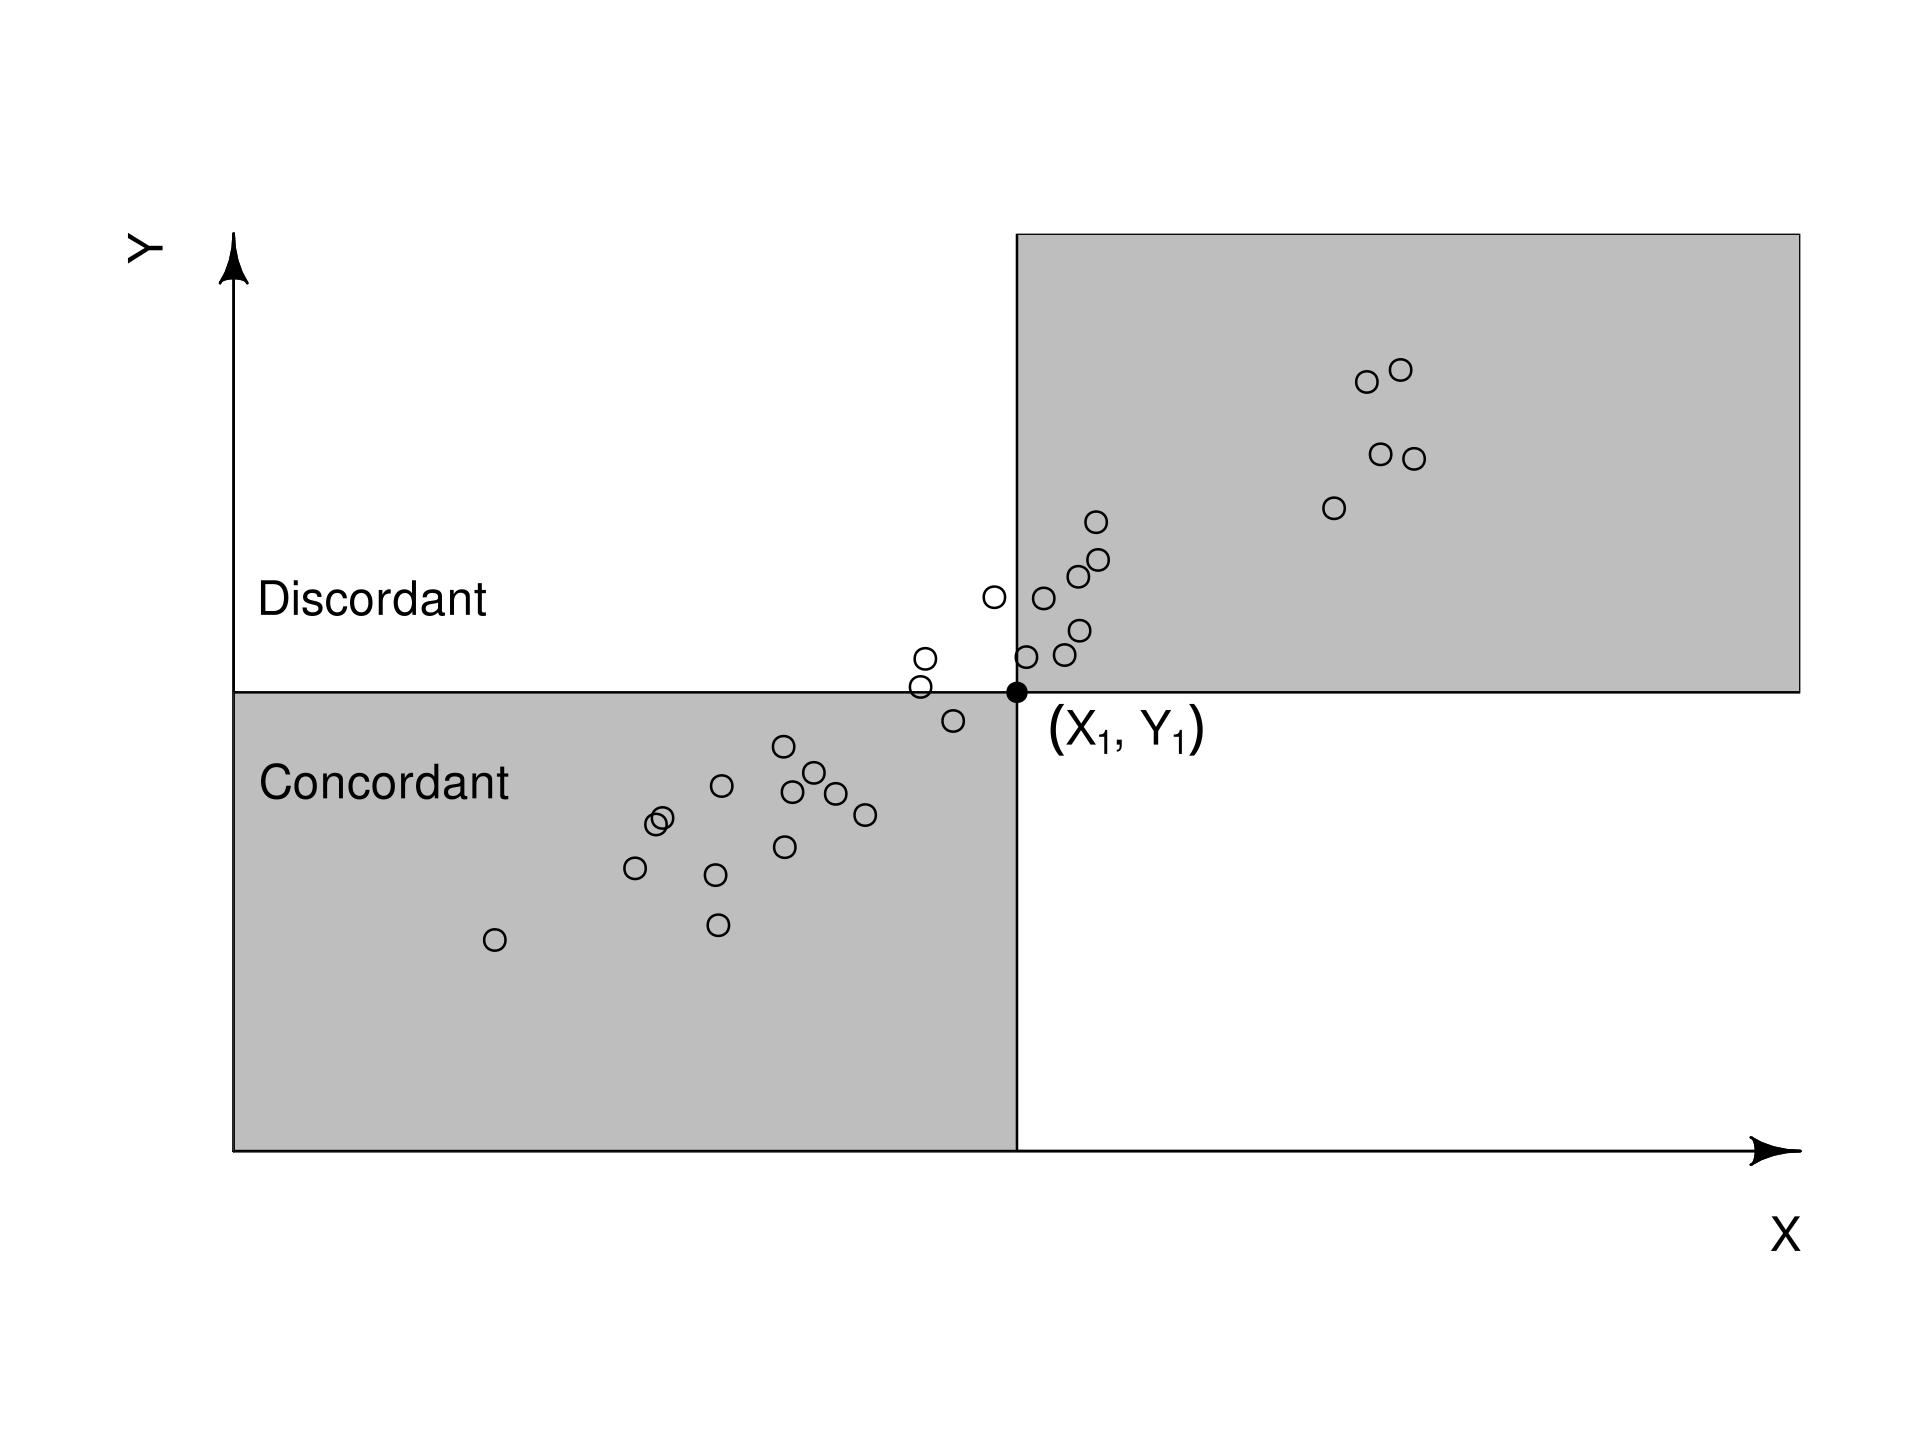
\includegraphics[width=0.5\textwidth]{figures/10-kendall-concordance.png}
  \caption{Kendall's $\tau$ 中一致与不一致的样本对。图片来自 \url{https://en.wikipedia.org/wiki/Kendall_rank_correlation_coefficient}}
  \label{fig:kendalls-tau}
\end{figure}

则 $\widehat\tau$ 本质上就是 $\tfrac{\text{一致样本对数}-\text{不一致样本对数}}{\text{总样本对数}}$ 。

\end{example}

\subsection{Mann--Whitney 统计量}

\begin{example}[Mann--Whitney 统计量]
这是一个两样本 U-统计量的例子。设 $X_1,\ldots,X_{n_1}\sim P$ i.i.d.、$Y_1,\ldots,Y_{n_2}\sim Q$ i.i.d.，且这些样本全体独立。``\textbf{\emph{Mann--Whitney 参数}}''考察 
$$\theta=P(X>Y)+\frac12 P(X=Y)$$
这个值经常用于假设检验，例如当 $X$ 来自``新药组''的某指标， $Y$ 来自``安慰剂组''，那么对假设 $\theta=0.5$ 进行检验能够判断两组是否存在系统性的区分。

取核函数 \[ h(x;y)=\mathbb I(x>y)+\frac12\mathbb I(x=y) \]两样本 U-统计量如下
\[\begin{aligned} U_{n_1,n_2}&=\frac1{n_1n_2}\sum_{j_1=1}^{n_1}\sum_{j_2=1}^{n_2}h(X_{j_1};Y_{j_2})\\ &=\frac1{n_1n_2}\sum_{j_1=1}^{n_1}\sum_{j_2=1}^{n_2}\Big(\mathbb I(X_{j_1}>Y_{j_2})+\frac12\mathbb I(X_{j_1}=Y_{j_2})\Big) \end{aligned}\]
将 $n_1n_2U_{n_1,n_2}$ 称作\textbf{\emph{Mann‑Whitney 统计量}} 。

\end{example}
\begin{remark}

\begin{itemize}
\tightlist
\item
  在机器学习领域的二分类问题中，如果记 $X_1,\dots,X_{n_1}$ 是分类器对正样本的打分、 $Y_1,\dots,Y_{n_2}$ 是对负样本打分，那么，基于这些样本绘制的 ROC 曲线，其\textbf{\emph{曲线下面积}} (AUC) 正是 $U_{n_1,n_2}$ 。例如，可参考早期文献 \cite{bamber1975}，或者机器学习相关资料，如 \cite{zhouzhihua2016} 的 §2.3.3 等。
\end{itemize}

% \href{https://www.zhihu.com/question/39840928}{如何理解机器学习和统计中的AUC？}

\begin{itemize}
\tightlist
\item
  如果将合样本 $X_1,\dots,X_{n_1},Y_1,\dots,Y_{n_2}$ 进行统一排序，并将每一样本在排序后的位次称作它的\textbf{\emph{秩 }}(rank)------当存在多个样本取相同的值，即所谓的 \textbf{\emph{结}} (ties)，我们用这些相同值样本的位次之平均作为它们的秩。即， $X_i$ 的秩为，
\end{itemize}
\[\begin{aligned} R_i &=\text{ 合样本中取值小于 $X_i$ 的个数} + \frac{\text{合样本中取值等于 $X_i$ 的个数} +1}2  \\&= \sum_{j_1=1}^{n_1} \mathbb{I}(X_{j_1} < X_i) \;+\; \sum_{j_2=1}^{n_2} \mathbb{I}(Y_{j_2} < X_i) \;+\; \frac{1}{2}\left( \sum_{j_1=1}^{n_1} \mathbb{I}(X_{j_1} = X_i) \;+\; \sum_{j_2=1}^{n_2} \mathbb{I}(Y_{j_2} = X_i) \;+\; 1 \right) \end{aligned}\]
那么，\textbf{\emph{Wilcoxon 秩和统计量}}定义为对所有 $X_i$ 的秩求和， $W_{n_1,n_2}=\sum_{i=1}^{n_1}R_i$。通过简单计算，我们得到\[\begin{aligned} W_{n_1,n_2} &= \sum_{j_1=1}^{n_1} \left( \sum_{k=1}^{n_1}\mathbb I(X_k<X_{j_1})+\sum_{l=1}^{n_2}\mathbb I(Y_l<X_{j_1})+\frac12\Biggl(\sum_{k=1}^{n_1}\mathbb I(X_k=X_{j_1})+\sum_{l=1}^{n_2}\mathbb I(Y_l=X_{j_1})+1\Biggr) \right) \\ &= \left(\sum_{j_1=1}^{n_1}\sum_{k=1}^{n_1}\mathbb I(X_k<X_{j_1})+\frac12\sum_{j_1=1}^{n_1}\sum_{k=1}^{n_1}\mathbb I(X_k=X_{j_1})\right) \\ &\qquad + \left(\sum_{j_1=1}^{n_1}\sum_{l=1}^{n_2}\mathbb I(Y_l<X_{j_1})+\frac12\sum_{j_1=1}^{n_1}\sum_{l=1}^{n_2}\mathbb I(Y_l=X_{j_1})\right) + \frac{n_1}{2} \\ &= \frac{n_1^2}{2} + \underbrace{\sum_{j_1=1}^{n_1}\sum_{l=1}^{n_2}\Bigl(\mathbb I(X_{j_1}>Y_l)+\frac12\mathbb I(X_{j_1}=Y_l)\Bigr)}_{=n_1n_2U_{n_1,n_2}} \;+\; \frac{n_1}{2} \\ &= n_1n_2U_{n_1,n_2} + \frac{n_1(n_1+1)}{2}. \end{aligned}\]这种统计量与 Mann‑Whitney 统计量仅相差一个 $\tfrac{n_1(n_1+1)}2$ ，因而二者在统计应用中可以视作是完全等价的。
\end{remark}


\subsection{最大均值差异 (MMD)}

本节是一个``齐一性检验''的例子，其目标是解决如下问题：给定取值于同一样本空间 $(\mathscr X,\mathscr B_x)$ 的两组独立样本 $X_1,\dots,X_{n_1}\sim P$ 、 $Y_1,\dots,Y_{n_2}\sim Q$ ，如何通过样本判断分布 $P$ 和 $Q$ 是否相同？

传统的方法，诸如 χ² 齐一性检验，对数据的限制太强，必须要求数据是有限离散的分离数据，对连续情况必须要分组处理；而且，这一方法也很难应用在高维的、结构复杂的数据上。\textbf{\emph{最大均值差异}} (Maximum Mean Discrepancy, MMD) 是一种基于核的距离度量，它通过将分布映射到\href{https://en.wikipedia.org/wiki/Reproducing_kernel_Hilbert_space}{再生核 Hilbert 空间}（RKHS）来比较它们之间的差异；原则上，只需要找到一个核 $k$ ，那么无论数据是连续或是高维，都可以定义出 MMD。

\begin{example}[最大均值差异（MMD）]\label{ex:ch10:mmd}
设 $\mathscr X$ 上有对称正定的核函数
\[k:\mathscr X\times \mathscr X\to\mathbb R\]
由 \href{https://en.wikipedia.org/wiki/Reproducing_kernel_Hilbert_space\#Moore\%E2\%80\%93Aronszajn_theorem}{Moore--Aronszajn 定理}，在 $\mathscr X$ 上存在唯一的 RKHS 空间 $\mathscr H_k$ 以 $k$ 为再生核。对每个分布 $P$ ，它在 $\mathscr H_k$ 中有均值嵌入 (mean embedding)：
\[
\mu_P=\mathbb E_{X\sim P}[k(\cdot,X)]=\int_{\mathscr X}k(\cdot,x)\mathrm{d}P(x).
\]

MMD 定义为两个嵌入之间的 Hilbert 空间距离：
\[
\mathrm{MMD}_k^2(P,Q)=\|\mu_P-\mu_Q\|^2_{\mathscr H_k}.
\]
在实践中，我们往往把范数平方展开，从而得到下面的形式：记独立样本 $X,X'\sim P$ 、 $Y,Y'\sim Q$ ，那么
\[
\mathrm{MMD}_k^2(P,Q) = \mathbb{E}_{X,X'\sim P}[k(X,X')] + \mathbb{E}_{Y,Y'\sim Q}[k(Y,Y')] - 2\mathbb{E}_{X\sim P, Y\sim Q}[k(X,Y)].
\]
为了配合上述形式，我们设两组样本是配对的：$(X_i, Y_i),~i=1,\ldots,n$，考虑 U-统计量核
\[
h_k^{(\mathrm{MMD})}\bigl((x_1,y_1), (x_2,y_2)\bigr) = k(x_1,x_2) + k(y_1,y_2) - k(x_1,y_2) - k(x_2,y_1).
\]
则 U-统计量如下：
\[\begin{aligned}\widehat{\mathrm{MMD}}_{k}^2 &= \binom{n}{2}^{-1} \sum_{1\le i<j\le n} h_k^{(\mathrm{MMD})}\bigl((X_i,Y_i), (X_j,Y_j)\bigr)\\ &= \frac{2}{n(n-1)} \sum_{1\le i<j\le n} k(X_i,X_j) \;+\; \frac{2}{n(n-1)} \sum_{1\le i<j\le n} k(Y_i,Y_j) \;-\; \frac{2}{n(n-1)} \sum_{1\le i<j\le n} \bigl(k(X_i,Y_j)+k(X_j,Y_i)\bigr)\\ &= \frac{2}{n(n-1)} \sum_{1\le i<j\le n} k(X_i,X_j) + \frac{2}{n(n-1)} \sum_{1\le i<j\le n} k(Y_i,Y_j) - \frac2{n(n-1)} \sum_{i\neq j} k(X_i,Y_j) \end{aligned}\]

我们后文中会回顾这个例子，该例的特点在于：在 $P=Q$ 的原假设下， $\mathrm{MMD}_k^2(P,Q)=0$ ，此时 $\widehat{\mathrm{MMD}}_{k}^2$ 是一阶退化的 U-统计量。

% 参考阅读：

% \href{https://www.zhihu.com/question/386309435/answer/1973074816077682003}{如何衡量两个「任意数据集」间的相似度？}

% \href{https://zhuanlan.zhihu.com/p/679276071}{迁移学习简介之最大均值差异（Maximum Mean Discrepancy）}

\end{example}

\subsection{Hilbert--Schmidt 独立性准则 (HSIC)}

上一节是一个齐一性检验的例子，本节我们来看看独立性检验。\textbf{\emph{Hilbert‑Schmidt 独立性准则}} 的基本思想和 MMD 类似，都是将分布放在 RKHS 空间中进行研究。

\begin{example}[Hilbert--Schmidt 独立性准则（HSIC）]\label{ex:ch10:hsic}
设 $X$ 取值于 $\mathscr X$、$Y$ 取值于 $\mathscr Y$，给定对称、正定的核函数
\[
k:\mathscr X\times \mathscr X\to \mathbb R,\quad l:\mathscr Y\times \mathscr Y\to \mathbb R.
\]
二者分别对应的 RKHS 记作 $\mathscr H_k$ 和 $\mathscr H_l$ 。定义联合分布 $P_{XY}$ 的均值嵌入为
\[\begin{aligned} \mu_{P_{XY}}&=\mathbb{E}_{X,Y}[k(\cdot,X)\otimes l(\cdot,Y)]\\ &=\int_{\mathscr X\times\mathscr Y}k(\cdot ,x)l(\cdot,y)\mathrm dP_{XY}(x,y) \end{aligned}\]
这里 $k(\cdot,X)\otimes l(\cdot,Y)$ 应该理解成一个二元函数：
\[
(x,y)\mapsto (k(\cdot,X)\otimes l(\cdot,Y))(x,y)=k(x,X)l(y,Y).
\]
而 $\mu_{P_{XY}}$ 实际上是 $\mathscr H_k\otimes \mathscr H_l$ 中的元素。

HSIC 定义为 \cite{gretton2005,gretton2008}：
\[
\mathrm{HSIC}_{k,l} = \|\mu_{P_{XY}} - \mu_{P_X} \otimes \mu_{P_Y}\|_{\mathscr{H}_k\otimes\mathscr{H}_l}^2.
\]

可见它其实就是 $P_{XY}$ 与 $P_X\otimes P_Y$ 在张量积空间 $\mathscr H_k\otimes \mathscr H_l$ 上的 MMD。展开范数平方，有下述更加简单的形式，
\[\begin{aligned} \mathrm{HSIC}_{k,l} &= \mathbb{E}_{X,X',Y,Y'}\bigl[k(X,X')l(Y,Y')\bigr] + \mathbb{E}_{X,X'}[k(X,X')]\mathbb{E}_{Y,Y'}[l(Y,Y')] - 2\mathbb{E}_{X,Y}\bigl[\mathbb{E}_{X'}[k(X,X')]\mathbb{E}_{Y'}[l(Y,Y')]\bigr]\\  \end{aligned}\]

对 $z_a = (x_a, y_a),\ a=1,2,3,4$ ，我们构造下面的四阶 U-统计量核 ：
\[\begin{aligned}h_{k,l}^{(\mathrm{HSIC})}(z_1, z_2, z_3, z_4) & = \frac{1}{4} h_k^{(\mathrm{MMD})}((x_1,x_3),(x_2,x_4)) h_l^{(\mathrm{MMD})}((y_1,y_3),(y_2,y_4))\\ &=\frac{1}{4} \Big(K_{12} + K_{34} - K_{14} - K_{23}\Big)\Big(L_{12} + L_{34} - L_{14} - L_{23}\Big)  \end{aligned}\]
其中 $K_{ij}=k(X_i,X_j)$ 代表 Gram 矩阵的 $i,j$ 元； $L_{ij}$ 同理；注意这个核非对称，那么 U-统计量应该写作
\[
\widehat{\mathrm{HSIC}}_{k,l}= \binom{n}{4}^{-1} \frac1{4!}\sum_{\substack{1\le j_1 , j_2 , j_3 , j_4 \le n\\ j_1,j_2,j_3,j_4\text{ 互不相同 }}} h_{k,l}^{(\text{HSIC})}(Z_{j_1}, Z_{j_2}, Z_{j_3}, Z_{j_4}).
\]
也可以用下面这个等价的对称核：
\[
h_{k,l}(Z_1,Z_2,Z_3,Z_4) = \frac{1}{4!}\sum_{\pi \in S_4} \Bigl(K_{\pi(1)\pi(2)} L_{\pi(1)\pi(2)} + K_{\pi(1)\pi(2)} L_{\pi(3)\pi(4)} - 2K_{\pi(1)\pi(2)} L_{\pi(1)\pi(3)}\Bigr).
\]

经过极其繁琐的展开， $\widehat{\mathrm{HSIC}}_{k,l}$ 最终能化简成\[\begin{aligned} \widehat{\mathrm{HSIC}}_{k,l} &= \frac{1}{n(n-1)} \sum_{1 \le j_1 \neq j_2 \le n} k(x_{j_1}, x_{j_2})\, l(y_{j_1}, y_{j_2}) \\ &\quad - \frac{2}{n(n-1)(n-2)} \sum_{\substack{1 \le j_1,j_2,j_3 \le n \\ j_1,j_2,j_3\ \text{互不相等}}} k(x_{j_1}, x_{j_2})\, l(y_{j_1}, y_{j_3}) \\ &\quad + \frac{1}{n(n-1)(n-2)(n-3)} \sum_{\substack{1 \le j_1,j_2,j_3,j_4 \le n \\ j_1,j_2,j_3,j_4\ \text{互不相等}}} k(x_{j_1}, x_{j_2})l(y_{j_3}, y_{j_4}). \end{aligned}\]
这个估计量可以参考 \cite{song2007,song2012}。


与例~\ref{ex:ch10:mmd} 相同，当 $X$ 和 $Y$ 独立时， $\mathrm{HSIC}_{k,l}=0$ ，可以证明 $\widehat{\mathrm{HSIC}}_{k,l}$ 也是一个退化的 U-统计量。

% 相关阅读：\href{https://spaces.ac.cn/archives/6910}{HSIC简介：一个有意思的判断相关性的思路 - 科学空间\textbar Scientific Spaces}。

\end{example}

\section{U-统计量的方差}

设 $X_1,\dots,X_m\sim P$ i.i.d.， U-统计量 $U_n$ 的核函数对称，并满足 $\mathbb E_P[h^2(X_1,\dots,X_m)]<\infty$ ，那么，令 $h_0=\theta=\mathbb E_P[h(X_1,\dots,X_m)]$

并对 $k=1,2,\dots,m$ ， 令
\[\begin{aligned} h_k(x_1,\dots,x_k)&=\mathbb E_P[h(x_1,\dots,x_k,X_{k+1},\dots,X_m)]\\ &=\mathbb E_P\Big[h(X_1,\dots,X_m)\ \Big|\  X_1=x_1,\dots,X_k=x_k\Big]\\ \end{aligned}\]
即固定前 $k$ 个变量，对剩余变量取平均。

将每个 $h_k$ 中心化，记
\[
\widetilde h_k(x_1,\dots,x_k)=h_{k}(x_1,\dots,x_k)-\theta.
\]
那么 $\mathbb E_P[h_k(X_1,\dots,X_k)]=0$ 。

再记
\[
\xi_k := \mathrm{Var}[h_k(X_1,\ldots,X_k)] = \mathbb{E}_P\Bigl[\widetilde{h}_k^2(X_1,\dots,X_k)\Bigr].
\]
在 $\mathbb E_P[h^2(X_1,\dots,X_m)]<\infty$ 的条件下，各 $\xi_k$ 是存在且有限的；实际上，易知方差随着固定变量数增加而单调不减
\[0 = \xi_0 \le \xi_1 \le \xi_2 \le \cdots \le \xi_m\]
这些 $\xi_k$ 衡量了 ``在已知 $k$ 个样本时，条件期望的变异程度''：
\begin{itemize}
\tightlist
\item
  若 $\xi_k$ 很大，说明 $k$ 个变量的观测会显著改变核 $h$ 的值，从而对 U-统计量产生较大的影响；
\item
  若 $\xi_k$ 很小，说明固定 $k$ 个变量后， $h$ 取值仍然接近于 $\theta$ ，不会发生较大的转变。
\end{itemize}

还有一点是，设 $\{1,\dots,n\}$ 的两组 $m$ 元指标子集 $I=\{\alpha_1,\dots,\alpha_m\}$ 和 $J=\{\beta_1,\dots,\beta_m\}$ 仅有 $k$ 个公共元素，那么
\[\begin{aligned} \mathrm{Cov}\big[ h(X_I),h(X_J)\big]&=\mathbb E\Big[\widetilde h(X_I)\widetilde h(X_J)\Big]\\ &=\mathbb E\Big[\mathbb E\Big[\widetilde h(X_I)\Big|X_{I\cap J}\Big]\mathbb E\Big[\widetilde h(X_J)\Big|I\cap J\Big]\Big]\\ &=\mathbb E\Big[\widetilde h^2_k(X_1,\dots,X_k)\Big]\\ &=\xi_k \end{aligned}\]
即：协方差仅依赖于指标集的公共元素个数。这是很关键的一步：当固定 $I$ 时，所有 $m$ 元指标子集 $J$ 中，与 $I$ 恰有 $k$ 个公共元的 $J$ 共有 $\binom mk\binom {n-m}{m-k}$个。通过以上这些准备，立即推出
\[\begin{aligned} \mathrm{Var}(U_n)&=\mathbb E_P\Big[(U_n-\mathbb E_P[U_n])^2\Big]\\ &= \binom{n}{m}^{-2} \sum_{I} \sum_{J} \mathrm {Cov}\bigl[h(X_I),h(X_J)\bigr]\\ &=\binom{n}{m}^{-2} \sum_I\sum_{k=1}^{m}\binom mk\binom{n-m}{m-k}\xi_k\\ &=\binom{n}{m}^{-1} \sum_{k=1}^{m}\binom mk\binom{n-m}{m-k}\xi_k \end{aligned}\]

我们写作定理。

\begin{theorem}[U-统计量的方差公式]
\label{thm:ch10:u-statistic-variance}

设 U -统计量的核 $h$ 对称，且 $\mathbb E[h^2(X_1,\dots,X_m)]<\infty$ ，那么由式~\eqref{eq:ch10a:tag-2} 定义的 U-统计量的方差为
\[\begin{aligned} \mathrm{Var}(U_n)=\binom{n}{m}^{-1} \sum_{k=1}^{m}\binom mk\binom{n-m}{m-k}\xi_k \end{aligned}\]
\end{theorem}

\begin{example}[样本方差的方差]
假定总体四阶矩有限，以 $\mu=\mathbb E_P[X]$ 记总体均值、 $\mu_k:=\mathbb E_P[(X-\mathbb E_P[X])^k]$ 记总体 $k$ 阶中心距，那么对 $h(x_1,x_2)=\tfrac{(x_1-x_2)^2}{2}$ ，有
\[\begin{aligned} h_1(x_1)&=\mathbb E_P[h(x_1,X_2)]=\frac12\mathbb E_P[(x_1-X_2)^2]\\ &=\frac12\mathbb E_P[(x_1-\mu)^2+(\mu-X_2)^2]\\ &=\frac12((x_1-\mu)^2+\mu_2) \end{aligned}\]
从而 \[ \xi_1=\mathrm{Var}[h_1(X_1)] = \frac14 \mathrm{Var}\!\big[(X_1-\mu)^2\big]=\frac{\mu_4-\mu_2^2}4 \]而
\[\begin{aligned} \xi_2&=\mathrm{Var}_P[h(X_1,X_2)] \\&= \mathbb{E}[h(X_1,X_2)^2] - (\mathbb{E}[h(X_1,X_2)])^2 \\ &= \frac14 \mathbb{E}[(X_1-X_2)^4] - \left( \frac12 \mathbb{E}[(X_1-X_2)^2] \right)^2 \\ &= \frac14 \mathbb{E}[((X_1-\mu)-(X_2-\mu))^4] - \mu_2^2 \\ &= \frac14 ( \mu_4 + 6\mu_2^2 + \mu_4 ) - \mu_2^2 \\ &= \frac{\mu_4 + \mu_2^2}{2} \end{aligned}\]
那么根据定理~\ref{thm:ch10:u-statistic-variance}，样本方差的方差为
\[\begin{aligned}\mathrm{Var}_P\left[\frac1{n-1}\sum_{j=1}^n(X_j-\bar X)^2\right]&=\binom{n}{2}^{-1} \sum_{k=1}^{2} \binom{2}{k} \binom{n-2}{2-k} \xi_k \\ &= \frac{4(n-2)}{n(n-1)}\xi_1 + \frac{2}{n(n-1)}\xi_2\\ &=\frac{\mu_4}{n} - \frac{n-3}{n(n-1)}\mu_2^2 \end{aligned}\]

\end{example}

\section{U-统计量的相合性}

利用方差公式容易得出如下推论

\begin{corollary}\label{cor:ch10:u-statistic-variance-order}
若 $\xi_1=\cdots=\xi_{r-1}=0$，$\xi_r>0$，那么
\[\mathrm{Var}[U_n]=\frac{r!}{n^r}{\binom mr}^2\xi_r+O\left(\frac1{n^{r+1}}\right)\]\end{corollary}

\begin{proof}

只需注意到对任意 $k=1,\dots,m$ ，定理~\ref{thm:ch10:u-statistic-variance} 中 $\xi_k$ 的系数
\[\begin{aligned} \binom{n}{m}^{-1} \binom mk\binom{n-m}{m-k}&=\frac{(n-m)!{\color{DarkRed}{m!}}}{n!}\frac{\color{DarkRed}{m!}}{\color{DarkRed}{k!(m-k)!}}\frac{(n-m)!}{{\color{DarkRed}{(m-k)!}}(n-2m+k)!}\\ &
  ={\color{DarkRed}{k!{\binom mk}^2}}\frac{(n-m)(n-m-1)\cdots(n-2m+k+1)}{n(n-1)\cdots (n-m+1)}\\ &=k!{\binom mk}^2\left(\frac1{n^k}+O\left(\frac1{n^{k+1}}\right)\right)\\ &=\frac{k!}{n^k}{\binom mk}^2+O\left(\frac1{n^{k+1}}\right) \end{aligned}\]
\end{proof}

这个推论告诉我们：

\begin{itemize}
\tightlist
\item
  若 $\xi_1>0$ ，那么方差至少以 $O(1/n)$ 的速率衰减，从而 $U_n-\theta=O_P(n^{-1/2})$ ；若 $\xi_1=0$ ，我们称 $U_n$ (一阶) 退化。
\item
  若 $\xi_1=0$ 但 $\xi_2>0$ ，那么方差至少以 $O(1/n^2)$ 的速率衰减，从而 $U_n-\theta=O_P(n^{-1})$ ；
\item
  依此类推，如果前 $r-1$ 项都为 0： $\xi_1=\cdots=\xi_{r-1}=0$ ，则方差至少以 $O(1/n^r)$ 衰减，从而 $U_n-\theta=O_P(n^{-r/2})$ 。
\end{itemize}
这论证了 $U_n\overset{P}\to \theta$ ，即 $U_n$ 是 (弱) 相合估计。

最后要补充的是： $U_n$ 不仅依概率收敛于 $\theta$ ，a.s. 收敛（强相合）也是成立的：

\begin{theorem}[U-统计量的强相合性]\label{thm:ch10:u-statistic-strong-consistency}

设 $\mathbb E_P[|h(X_1,\dots,X_n)|]<\infty$ ，那么 $U_n\overset{\text{a.s.}}\to\theta$ 。

\end{theorem}

\begin{remark}
U-统计量强相合性的原始结果可参见 \cite{berk1966} 与 \cite{arvesen1969}。定理~\ref{thm:ch10:u-statistic-strong-consistency} 有多种证明方法，例如 \cite{lee1990} 一书的 §3.4 就给出了三种不同的证明。限于篇幅，我们这里介绍其中最为简洁优雅的第三种证明。亦可参考~\cite{chenxiru2012} 的 §2.4.1 。
\end{remark}

\begin{proof}

对任意 $\epsilon > 0$ ，定义
\[\begin{aligned} U(\epsilon) &:= \bigl\{ U_n > \theta + \epsilon \text{ 发生无穷多次} \bigr\}\\ L(\epsilon) &:= \bigl\{ U_n < \theta - \epsilon \text{ 发生无穷多次} \bigr\} \end{aligned}\]
用集合论的语言，
\[\begin{aligned} U(\epsilon) &= \bigcap_{n=1}^{\infty} \bigcup_{m=n}^{\infty} \{ U_m > \theta + \epsilon \}\\ L(\epsilon) &= \bigcap_{n=1}^{\infty} \bigcup_{m=n}^{\infty} \{ U_m < \theta + \epsilon \}\\  \end{aligned}\]
由于 U-统计量 $U_n$ 的性质，上面两个事件都是可排列的 (permutable)，即，只对有限多个 $X_j$ 交换次序，那么对足够大的 $m$ ，U-统计量 $U_m$ 是不发生改变的，从而不影响``发生无穷多次''。由 \href{https://en.wikipedia.org/wiki/Hewitt\%E2\%80\%93Savage_zero\%E2\%80\%93one_law}{Hewitt‑Savage 0‑1 律}， $U(\epsilon)$ 和 $L(\epsilon)$ 的概率要么是 0 要么是 1；这里的``概率''视作是 $X$ 所在概率空间的无穷乘积空间上的概率测度。

设 $T_n:=\{X_{(1)},\dots,X_{(n)}\}$ 是次序统计量，考虑 $\sigma$-代数族
\[
\mathscr F_n:=\sigma(T_n,X_{n+1},X_{n+2},\dots).
\]

那么 $\mathscr F_n\supset \mathscr F_{n+1}$，于是\[ U_{n+1}=\mathbb E_P[h(X_1,\dots,X_m)\mid T_{n+1}]=\mathbb E_P[h(X_1,\dots,X_m)\mid \mathscr F_{n+1}]=\mathbb E_P[U_n\mid \mathscr F_n]\quad \text{a.s.} \]

可知 $U_n$ 构成反向鞅 (Reverse Martingale)，由鞅收敛定理，存在随机变量 $U_\infty$ 使得
\[
U_n \xrightarrow{\text{a.s. 且 } L_1} U_\infty \quad \text{ 当 } n \to \infty.
\]

由于 $\mathbb{E}[U_n] = \theta$ ，不可能以概率 1 发生 $U_n > \theta + \epsilon$ 无穷多次，如若不然，
\[ \theta = \lim_{n\to\infty} \mathbb{E}[U_n]=\mathbb E[U_\infty]\ge \theta + \epsilon \]矛盾。所以 $U(\epsilon)$ 发生的概率是 0，同理， $L(\epsilon)$ 亦如此。而`` $U_n$ 不收敛于 $\theta$ ''的样本点可以表示为 $\bigcup_{k=1}^{\infty} \bigl( U(1/k) \cup L(1/k) \bigr)$ ，这发生的概率仍然是 0。

\end{proof}

% Generated from: Zhihu/专栏：概率与统计/渐近统计 (10)：U-统计量 (下)_金鱼马_2026-06-06.md
% 本篇延续上一部分，定理和公式编号也随之顺延。前一部分主要讨论了 U-统计量的概念、应用、方差公式，最后简单介绍了相合性。本篇主要解决渐近统计中更加感兴趣的话题：U-统计量的渐近正态性。

\section{U-统计量的渐近正态性}

我们从推论~\ref{cor:ch10:u-statistic-variance-order} 中看到的是：U-统计量方差的收敛速度与它是否退化有关，

\begin{itemize}
\tightlist
\item
  对``非退化''情况，即 $\xi_1>0$ 时， $\mathrm{Var}[U_n]=O(1/n)$ ， $U_n-\theta=O_P(n^{-1/2})$ ；
\item
  对``(一阶) 退化''情况，即 $\xi_1=0$ 、 $\xi_2>0$ 时， $\mathrm{Var}[U_n]=O(1/n^2)$ ， $U_n-\theta=O_P(n^{-1})$ ；
\item
  以此类推，当 $\xi_1=\cdots=\xi_{r-1}=0$ 、 $\xi_r>0$ 时， $\mathrm{Var}[U_n]=O(1/n^r)$ ， $U_n-\theta=O_P(n^{-r/2})$ 。
\end{itemize}

这当然也会影响最终 $U_n$ 渐近分布。事实上，只有非退化的情形， $U_n$ 才是渐近正态的；对于 (一阶) 退化的情况， $U_n$ 的渐近分布会变成无限个 χ² 分布的加权和。

当我们想分析 $U_n$ 统计量的渐近分布时，一个重要的麻烦是，由式~\eqref{eq:ch10b:tag-2} 所定义的 $U_n$ ，

\begin{equation}
\label{eq:ch10b:tag-2}
U_n=\binom nm^{-1}\sum_{1\le j_1<\cdots<j_m\le n}h(X_{j_1},\dots,X_{j_m})
\end{equation}

由于样本的诸 m-元子集存在重叠，导致 $h(X_{j_1},\dots,X_{j_m})$ 并不相互独立，没法用诸如独立随机变量和中心极限独立的工具。为此，Hoeffding 提出了``投影''的方法。

\subsection{Hájek 投影}

所谓``投影''，指的是将 $U_n$ 投影到每个 $X_j$ 所张成的空间上，也就是

\begin{equation}
\label{eq:ch10b:tag-3}
\widetilde{U}_n = \mathbb{E}[U_n] + \sum_{j=1}^n \bigl( \mathbb{E}[U_n| X_j] - \mathbb{E}[U_n] \bigr)
\end{equation}

由于 $X_i$ 相互独立，$\mathbb{E}[U_n| X_i]$ 也是独立的，因此 $\widetilde{U}_n$ 是独立随机变量（加上常数）的线性组合，可以直接使用中心极限定理，提供正态性。在此基础上，若能够证明 $U_n$ 与 $\widetilde{U}_n$ 在适当的归一化下，其差值可以忽略，那么 $U_n$ 的渐近分布就由 $\widetilde{U}_n$ 完全决定。

为什么它被称作``投影''呢？设每个 $X_j$ 均取值于样本空间 $(\mathscr X,\mathscr B_x)$ ，我们记在 $n$ 个样本的乘积空间上、全体平方可积函数记作 $L^2$ ，这是一个 Hilbert 空间，内积为
\[
\langle f,g\rangle
=\mathbb E[f(X_1,\dots,X_n)g(X_1,\dots,X_n)].
\]
在 Hilbert 空间中，我们可以对每个元素向其闭子空间进行正交投影，这里要研究的闭子空间 $\mathscr S_n$ 定义如下：它是全体形如
\[\sum_{j=1}^ng_j(X_j)\]
的统计量张成的空间，其中每个 $g_j$ 是平方可积的可测函数（ $\mathbb E[g_j^2(X)]<\infty$ ）。简而言之，这类统计量完全由每个样本独立的贡献相加而成。显然 $\mathscr S_n$ 是 $L^2$ 的线性闭子空间。

\begin{lemma}[Hájek 投影]\label{lem:ch10:hajek-projection}

设独立样本 $X_1,\dots,X_n$ 取值于样本空间 $(\mathscr X,\mathscr B_x)$，$T=T(X_1,\dots,X_n)$ 是任意满足 $\mathbb E[T^2]<\infty$ 的统计量。那么，$T$ 向 $\mathscr S_n$ 进行投影所得到的便是
\[
\begin{aligned}
\widetilde T
&=\mathbb E[T]+\sum_{j=1}^n(\mathbb E[T|X_j]-\mathbb E[T])\\
&=\sum_{j=1}^n\mathbb E[T|X_j]-(n-1)\mathbb E[T].
\end{aligned}
\]

换言之，对任意 $S\in\mathscr S_n$ ，有 $\mathbb E[(T-\widetilde T)S]=0$ 。

\end{lemma}

\begin{proof}

注意到（在 a.s. 的意义上）有
\[\begin{aligned} \mathbb E[\widetilde T|X_j]&=\sum_{i=1}^n\mathbb E\Big[\mathbb E[T|X_i]\Big|X_j\Big]-(n-1)\mathbb E[T]\\ &=(n-1)\mathbb E[T]+\mathbb E[T|X_j]-(n-1)\mathbb E[T]\\ &=\mathbb E[T|X_j] \end{aligned}\]
从而
\[\begin{aligned} \mathbb E[(T-\widetilde T)S]&=\mathbb E\left[(T-\widetilde T)\sum_{j=1}^ng_j(X_j)\right]\\ &=\sum_{j=1}^n\mathbb E[(T-\widetilde T)g_j(X_j)]\\ &=\sum_{j=1}^n\mathbb E\big[g_j(X_j)\mathbb E[(T-\widetilde T)|X_j]\big]\\ &=\sum_{j=1}^n\mathbb E\Big[g_j(X_j)\big(\underbrace{\mathbb E[T|X_j]-\mathbb E[\widetilde T|X_j]}_{0}\big)\Big]\\ &=0 \end{aligned}\]
\end{proof}

如果 $X_1,\dots,X_n$ 是 i.i.d. 的，且 $T=T(X_1,\dots,X_n)$ 是对称的，那么对每个 $j$ ，
\[
\mathbb E[T|X_j=x]=\mathbb E[T|X_1=x]=\mathbb E[T(x,X_2,\dots,X_n)].
\]

是不依赖于 $j$ 的。我们便可以对 Hájek 投影用经典 i.i.d. 条件下的中心极限定理。

另一个要解决的问题是，投影 $\widetilde T$ 是否能足够接近 $T$ 呢？见下，

\begin{lemma}[投影逼近]\label{lem:ch10:hajek-approximation}

设 $T_n=T_n(X_1,\dots,X_n)$ 是任意 $\mathbb E[T_n^2]<\infty$ 的统计量， $\mathscr S\subset L^2$ 是任一包含常数的闭子空间， $T_n$ 向 $\mathscr S$的投影为 $\widetilde T\!_n$ 。那么，若
\[
\mathrm{Var}[T_n]-\mathrm{Var}[\widetilde T\!_n]=o(1/n),
\]

则
\[
\sqrt n(T_n-\widetilde T_n)\overset{L^2}\longrightarrow 0.
\]

\end{lemma}

\begin{proof}

首先由投影的正交性知
\[
\mathbb{E}\big[(T_n - \widetilde{T}\!_n)\widetilde{T}\!_n\big] = 0,\quad \mathbb{E}\big[(T_n - \widetilde{T}\!_n)1\big] = 0.
\]

从而 $T_n-\widetilde T\!_n$ 和 $\widetilde T\!_n$ 不相关：
\[\mathrm{Cov}[T_n-\widetilde T\!_n,\widetilde T\!_n]=\underbrace{\mathbb E\big[(T_n-\widetilde T\!_n)\widetilde T\!_n\big]}_{0}-\mathbb E\big[\widetilde T\!_n\big]\underbrace{\mathbb E\big[T_n-\widetilde T\!_n\big]}_{0}=0\]
那么方差满足
\[
\mathrm{Var}[T_n]=\mathrm{Var}[\widetilde T\!_n]+\mathrm{Var}\big[T_n-\widetilde T\!_n\big].
\]

因此
\[
n\mathbb E\big[(T_n-\widetilde T\!_n)^2\big]=n\mathrm{Var}\big[T_n-\widetilde T\!_n\big]=n\big(\mathrm{Var}[T_n]-\mathrm{Var}[\widetilde T_n]\big)=n\cdot o(1/n)=o(1)\longrightarrow 0.
\]

\end{proof}

下面我们将这套方法用在 U-统计量上。

\subsection{非退化情形下的渐近正态性}

对于参数 $\theta$ 的 U-统计量 $U_n$ ，
\[\begin{aligned} \mathbb E[U_n|X_j]&=\binom nm^{-1}\mathbb E\left[\sum_{1\le j_1<\cdots<j_m\le n}h(X_{j_1},\dots,X_{j_m})\Bigg|X_1\right]\\ &=\binom nm^{-1}\mathbb E\Bigg[\sum_{\substack{j_1>1\\j_1< j_2<\cdots<j_m\le n}}h(X_{j_1},\dots,X_{j_m})+\sum_{\substack{j_1=1\\j_1< j_2<\cdots<j_m\le n}}h(X_{j_1},\dots,X_{j_m})\Bigg|X_1\Bigg]\\ &= {\binom{n}{m}}^{-1}\left( \binom{n-1}{m}\theta + \binom{n-1}{m-1} h_1(X_j) \right)\\ &=\frac{n-m}{n}\theta + \frac{m}{n} h_1(X_j) \end{aligned}\]
所以根据式~\eqref{eq:ch10b:tag-3} ，它的 Hájek 投影是

\begin{equation}
\label{eq:ch10b:tag-4}
\widetilde{U}_n = \theta + \sum_{j=1}^n \bigl( \mathbb{E}[U_n|X_j] - \theta \bigr) = \theta + \frac{m}{n}\sum_{j=1}^n \bigl( h_1(X_j) - \theta \bigr)
\end{equation}

这里可以看出非退化要求的必要性，因为
\[
\mathrm{Var}[\widetilde U_n]=\left(\frac mn\right)^2\cdot n\mathrm{Var}[h_1(X)]=\frac{m^2}n\xi_1.
\]

如果 $\xi_1=0$ （退化），那么 $\widetilde U_n=\theta$ 几乎处处，这意味着一阶信息完全缺失，U‑统计量渐近分布的主导项必然来自更高阶的投影。

现设 $\xi_1>0$ （非退化），那么我们可以放心对式~\eqref{eq:ch10b:tag-4} 用经典中心极限定理：
\[
\sqrt n(\widetilde U-\theta)\overset{\rm d}\to \mathcal N(0,m^2\xi_1).
\]

而另一方面，推论~\ref{cor:ch10:u-statistic-variance-order} 告诉我们
\[
\mathrm{Var}[U_n]=\frac{m^2}{n}\xi_1+O\left(\frac1{n^2}\right)=\mathrm{Var}[\widetilde U_n]+O\left(\frac1{n^2}\right).
\]

所以根据引理~\ref{lem:ch10:hajek-approximation}， $\sqrt{n}(U_n-\widetilde U_n)$ 均方收敛到 0，自然也依概率收敛到 0：
\[
P(\sqrt n|U_n-\widetilde U_n|>\epsilon)\le\frac{n\mathbb E[(U_n-\widetilde U_n)^2]}{\epsilon^2}\to 0.
\]

从而就证明了我们想要的结论：
\[\begin{aligned} \sqrt n(U_n-\theta)&=\sqrt n(\widetilde U_n-\theta)+\sqrt n(U_n-\widetilde U_n)\\ &=\sqrt n(\widetilde U_n-\theta)+o_P(1)\\ &\overset{\rm d}\to\mathcal N(0,m^2\xi_1) \end{aligned}\]
我们写作定理：

\begin{theorem}[U-统计量的渐近正态性：非退化情形]\label{thm:ch10:u-statistic-nondegenerate-clt}

设 $U_n$ 是基于 i.i.d. 样本 $X_1,\dots,X_n\sim P$ 的 U-统计量，核函数 $h(X_1,\dots,X_m)$ 对称且 $\mathbb E[h^2(X_1,\dots,X_m)]<\infty$ 。若 \[ \xi_1:=\mathrm{Var}_P[h_1(X)]=\mathrm{Var}_P\big[\mathbb{E}_P[h(X_1,X_2,\dots,X_m)|X_1]\big] \]满足 $0<\xi_1<\infty$ ，那么
\[\sqrt n(U_n-\mathbb E_P[U_n])\overset{\rm d}\longrightarrow \mathcal N(0,m^2\xi_1)\]
\end{theorem}

下面简单举一个利用定理~\ref{thm:ch10:u-statistic-nondegenerate-clt} 的应用例子。在非退化情形（$\xi_1 > 0$）下，要找 $\theta=\mathbb E[U_n]$ 的渐近置信区间，若已知 $\xi_1$，则直接有渐近水平为 $1-\alpha$ 的置信区间为
\[U_n \pm z_{1-\alpha/2}\, \frac{m\sqrt{\xi_1}}{\sqrt{n}}\]
其中 $z_{1-\alpha/2}$ 是标准正态分布的上 $1-\alpha/2$ 分位数。然而问题在于， $\xi_1 = \mathrm{Var}[h_1(X)]$ 依赖于未知的总体分布 ，除非特殊情况，我们是不知道 $\xi_1$ 的真实值的，必须想办法从样本中估计 $\xi_1$。

对每个观测 $X_i$，考虑所有包含 $i$ 的 $m$ 元组，并计算这些核函数值的平均：
\[\widehat{h}_{1,i} = \binom{n-1}{m-1}^{-1} \sum_{\substack{A\subseteq\{1,\dots,n\}\\ |A|=m,\; i\in A}} h(X_A)\]
这个量称为\emph{留一平均}（leave‑one‑in average），因为它固定了 $X_i$，而对其他 $m-1$ 个位置在所有可能的组合上平均。由 U‑统计量的无偏性，
\[\mathbb{E}\bigl[\widehat{h}_{1,i}\bigr] = h_1(X_i).\]
表明 $\widehat{h}_{1,i}$ 是 $h_1(X_i)$ 的一个无偏估计。在此基础上，可构造 $\xi_1 = \mathrm{Var}[h_1(X)]$ 的估计：
\[\widehat{\xi}_1 = \frac{1}{n-1}\sum_{i=1}^n \bigl(\widehat{h}_{1,i} - U_n\bigr)^2\]
可以证明 $\widehat{\xi}_1$ 是 $\xi_1$ 的相合估计：$\widehat{\xi}_1 \overset P\to \xi_1$，于是可将
\[U_n \pm z_{1-\alpha/2}\frac{m\sqrt{\widehat{\xi}_1}}{\sqrt{n}}\]
作为渐近 $1-\alpha$ 置信区间。

类似地，对于检验 $H_0:\theta = \theta_0$，若原假设下统计量非退化，则可构造检验统计量
\[Z_n = \frac{\sqrt{n}\,(U_n - \theta_0)}{m\sqrt{\widehat{\xi}_1}} \overset{\rm d}\to\mathcal{N}(0,1)\]
在显著性水平 $\alpha$ 下，当 $|Z_n| > z_{1-\alpha/2}$ 时拒绝 $H_0$。

不过，U-统计量可能是退化的（如例~\ref{ex:ch10:mmd} 和例~\ref{ex:ch10:hsic}），导致上述正态近似无效，甚至 $\sqrt{n}$ 的缩放也是错误的；要特别声明，U-统计量的退化不是仅仅理论上的病态，在实际中，退化是很常见的。接下来我们讲解退化 U-统计量的渐近理论。

\subsection{Hoeffding 分解}

接下来研究 $\xi_1=0$ 、 $\xi_2>0$ 的情形，我们称这样的 U‑统计量为一阶退化的。注意到，此时 $U_n$ 的 Hájek 投影 $\widetilde U_n$ 几乎处处是常数，无法为我们提供任何信息。因此，将``Hájek 投影''这一概念推广到高阶，是很有必要的。

（本节的细节比较繁琐，读者可以跳过，只需承认推论~\ref{cor:ch10:hoeffding-decomposition} 即可。）

Hájek 投影之所以是一个``一阶''的概念，是因为它将统计量表述为一个样本 $X_j$ 的函数 $g_j(X_j)$ 的求和。我们需要将其推广成二元、三元等多元函数。为此，对任一 $A\subset\{1,\dots,n\}$ ，定义 $H_A$ 是全体形如 $g_A(X_j:j\in A)$

的统计量张成的子空间，其中 $g_A$ 是平方可积的可测函数，且满足退化条件：
\[\mathbb E\big[g_A(X_j:j\in A)\ \big|\ X_j:j\in B\big]=0,\quad \forall\ |B|<|A|\]
（特别定义 $\mathbb E[T|\emptyset]=\mathbb E[T]$ )

即： $g_A$ 只用来捕捉 $|A|$ 个元素的共同信息，或者叫 $|A|$ 阶信息；而对任何 $|B|<|A|$ ， $g_A$ 不包含 $|B|$ 阶信息。由于 $X_j$ 的独立性，这里的 $B$ 可以推广到任意不包含 $A$ 的子集，于是，上述退化条件保证了不同子集对应的空间是正交的，整个空间可以分解成 $L^2=\bigoplus_{A\subset \{1,\dots,n\}}H_A$

那么任何 $T\in L^2$ 都可以唯一地向每个子空间进行投影，并表示为所有投影之和。若记 $P_AT$ 表示 $T$ 向 $H_A$ 的投影，则
\[T=\sum_{A\subset\{1,\dots,n\}}P_AT\]
特别地，

\begin{itemize}
\tightlist
\item
  $P_\emptyset T=\mathbb E[T]$ ；
\item
  $P_{\{j\}}T=\mathbb E[T|X_j]-\mathbb E[T]$ ；
\item
  $P_{\{i,j\}}T=\mathbb E[T|X_i,X_j]-\mathbb E[T|X_i]-\mathbb E[T|X_j]+\mathbb E[T]$ ；
\item
  \ldots{}
\end{itemize}

可见，Hájek 投影只是对应 $\textstyle P_\emptyset T+\sum_{j=1}^nP_{\{j\}}T$ 。而一般地，如果我们想明确写出某个 $P_AT$ 的表达式，有如下结论，

\begin{lemma}[子集上的正交投影]\label{lem:ch10:subset-projection}

设 $X_1,\dots,X_n$ 独立，对任意子集 $A\subset\{1,\dots,n\}$ 和任意平方可积的统计量 $T=T(X_1,\dots,X_n)$ ， $T$ 向 $P_A$ 的投影是
\[P_AT=\sum_{B\subset A}(-1)^{|A|-|B|}\mathbb E\big[T\big|X_j:j\in B\big]\]
\end{lemma}

\begin{proof}

简洁起见，记 $\mathbb E_B[T]:=\mathbb E[T|X_j:j\in B]$ 。证明分两步，

\begin{itemize}
\tightlist
\item
  首先证明 $P_AT\in H$ 。我们需要验证：对任意 $C \subsetneq A$，有 $\mathbb E_C[P_AT]=0$ 。代入 $P_AT$ ，
\[\begin{aligned} \mathbb E_C[P_AT]&= \sum_{B\subset A} (-1)^{|A|-|B|} \mathbb E_{B\cap C} [T]\\ &=\sum_{D\subset C}\sum_{E\subset A\setminus C}(-1)^{|A|-|D|-|E|}\mathbb E_D[T]\\ &=\left(\sum_{D\subset C}(-1)^{|A|-|D|}\mathbb E_D[T]\right)\left(\sum_{E\subset A\setminus C}(-1)^{|E|}\right)\\ &=\left(\sum_{D\subset C}(-1)^{|A|-|D|}\mathbb E_D[T]\right)(1-1)^{|A\setminus C|}\\ &=0 \end{aligned}\]
其中第四行来自二项式定理。

\item
  其次证明 $T-P_AT$ 与 $H_A$ 正交。任取 $g_A=g_A(X_j:j\in A)\in H_A$ ，
\[\begin{aligned} \mathbb{E}\bigl[(T-P_A T)g_A\bigr] &= \mathbb{E}\bigl[(T-\mathbb{E}_A[T])g_A\bigr] - \sum_{B\subsetneq A} (-1)^{|A|-|B|} \mathbb{E}\bigl[\mathbb{E}_B[T] \, g_A\bigr] \\ &= \underbrace{\mathbb{E}\bigl[(T-\mathbb{E}_A[T])g_A\bigr]}_0 - \sum_{B\subsetneq A} (-1)^{|A|-|B|} \mathbb{E}\Bigl[\mathbb{E}_B[T] \  \underbrace{\mathbb{E}_B[g_A]}_{0}\Bigr] \\ &= 0 \end{aligned}\]
\end{itemize}

\end{proof}

接下来设 $X_1,\dots,X_n$ 独立同分布，且 $T(X_1,\dots,X_n)$ 是对称函数，那么由对称性， $P_AT$ 仅依赖于 $|A|$ 的大小，因此对 $|A|=r$ ，可以记 $P_AT=g_r(X_j:j\in A)$ ；根据引理~\ref{lem:ch10:subset-projection}，这里的 $g_r$ 可以显式写出
\[\begin{aligned} g_r(X_j:j\in A)&=\sum_{A\subset\{1,\dots,r\}}(-1)^{r-|A|}\mathbb E[T|X_j:j\in A]\\ &=\sum_{c=0}^r(-1)^{r-c}\sum_{1\le j_1<\cdots<j_c\le r}\mathbb E[T|X_{j_1},\dots,X_{j_c}] \end{aligned}\]
可见 $g_r$ 也是对称函数。那么
\[\begin{aligned} T&=\sum_{A\subset\{1,\dots,n\}}P_AT=\sum_{r=0}^n\sum_{|A|=r}g_r(X_j:j\in A)\\ &=\mathbb E[T]+\sum_{j=1}^ng_1(X_j)+\sum_{1\le j_1<j_2\le n}g_2(X_{j_1},X_{j_2})+\sum_{1\le j_1<j_2<j_3\le n}g_3(X_{j_1},X_{j_2},X_{j_3})+\cdots+g_n(X_1,\dots,X_n) \end{aligned}\]
这便是 \textbf{\emph{Hoeffding 分解}} 。

放在 U-统计量的情境下，我们将式~\eqref{eq:ch10b:tag-2} 中的每个核 $h(X_{j_1},\dots,X_{j_m})$ 进行 Hoeffding 分解，注意到

\begin{itemize}
\tightlist
\item
  $r=0$ 项是 $\theta$ ；
\item
  当 $|A|=r>m$ 时， $h(X_{j_1},\dots,X_{j_m})$ 与每个 $H_A$ 都正交；
\item
  所以只需将 $h(X_{j_1},\dots,X_{j_m})-\theta$ 写作对 $r=1,\dots,m$ 的求和形式。
\end{itemize}

所以式~\eqref{eq:ch10b:tag-2} 推出
\[\begin{aligned} U_n - \theta  &= \binom{n}{m}^{-1} \sum_{1\le j_1<\cdots<j_m\le n} (h(X_{j_1},\dots,X_{j_m}) -\theta)\\ &= \binom{n}{m}^{-1} \sum_{1\le j_1<\cdots<j_m\le n} \; \sum_{r=1}^{m} \; \sum_{\substack{A\subset\{j_1,\dots,j_m\}\\ |A|=r}} P_A h(X_{j_1},\dots,X_{j_m}) \\ &= \binom{n}{m}^{-1} \sum_{r=1}^{m} \; \sum_{1\le j_1<\cdots<j_m\le n} \; \sum_{\substack{A\subset\{j_1,\dots,j_m\}\\ |A|=r}} g_r(X_A) \\ &= \binom{n}{m}^{-1} \sum_{r=1}^{m} \; \sum_{|A|=r} g_r(X_A) \cdot \binom{n-r}{m-r} \\ &= \sum_{r=1}^{m} \binom{m}{r}{\binom{n}{r}}^{-1} \sum_{|A|=r} g_r(X_A) \\  \end{aligned}\]
其中 $g_r(X_A):=g_r(X_j:j\in A)=P_Ah(X_{j_1},\dots,X_{j_m})$ 。

我们写作引理，

\begin{lemma}[U-统计量的 Hoeffding 分解]\label{lem:ch10:u-statistic-hoeffding-decomposition}

设参数 $\theta$ 的 U-统计量是 $U_n$ ，其核 $h(X_1,\dots,X_m)$ 对称且 $\mathbb E[|h(X_1,\dots,X_m)|]<\infty$ ，那么
\[
U_n-\theta=\sum_{r=1}^m\binom mr\widetilde U_{n,r}.
\]

其中 $\widetilde U_{n,r}$ 是一个以 $g_r(x_1,\dots,x_r)$ 为核、期望为 0 的 U-统计量，
\[g_r(x_1,x_2,\dots,x_r)=\sum_{c=0}^r(-1)^{r-c}\sum_{1\le j_1<\cdots<j_c\le r}h_c(x_{j_1},\dots,x_{j_c}),\quad r=1,\dots,m\]
这里 $h_c$ 定义同前文： $h_0=\theta$ 、 $h_r(x_1,\dots,x_r)=\mathbb E[h(x_1,\dots,x_r,X_{r+1},\dots,X_{m})]$ ， $r=1,\dots,m$ 。

我们继续利用退化性质：核 $g_r$ 满足：对任意的 $c<r$ ，
\[
\mathbb E[g_r(x_1,\dots,x_c,X_{c+1},\dots,X_r)]=\mathbb E[g_r(X_1,\dots,X_r)|X_1=x_1,\dots,X_c=x_c]=0.
\]

因此，当 $r\ge 2$ 时，引理~\ref{lem:ch10:u-statistic-hoeffding-decomposition} 中的每个 $U_{n,r}$ 都是 $r-1$ 阶退化的 U-统计量。根据推论~\ref{cor:ch10:u-statistic-variance-order}，
\[
\mathrm{Var}[\widetilde U_{n,r}]=\frac{r!}{n^r}\mathrm{Var}[g_r(X_1,\dots,X_r)]+O\left(\frac1{n^{r+1}}\right).
\]

特别地，在 U-统计量 $r-1$ 阶退化时，我们展开到 $r$ 阶项，能得到如下结论：

\end{lemma}

\begin{corollary}[Hoeffding 分解]\label{cor:ch10:hoeffding-decomposition}
若 $U_n$ 一阶退化，即 $\xi_1=\mathrm{Var}[h_1(X)]=0$，那么 $U_n-\theta=\binom m2\widetilde U_{n,2}+R_n$。

其中
\[
\widetilde U_{n,2}=\binom n2^{-1}\sum_{1\le j_1<j_2\le n}(h_2(X_{j_1},X_{j_2})-\theta).
\]

是一个均值为 0 的、一阶退化的 U-统计量；余项 $R_n$ 满足 $\mathbb E[R_n]=0$ 、 $\mathrm{Var}[R_n]=O(n^{-3})$ 。

更一般地，若 $U_n$ 是 $r-1$ 阶退化的，即 $\xi_1=\cdots=\xi_{r-1}=0$ ，那么 $U_n-\theta=\binom mr\widetilde U_{n,r}+R_n$

其中
\[
\widetilde U_{n,r}=\binom nr^{-1}\sum_{1\le j_1<\cdots<j_r\le n}(h_r(X_{j_1},\dots,X_{j_r})-\theta).
\]

是一个均值为 0 的、$r-1$ 阶退化的 U-统计量。余项 $R_n$ 满足 $\mathbb E[R_n]=0$、$\mathrm{Var}[R_n]=O(n^{-r-1})$。
\end{corollary}

\subsection{积分算子与谱分解}

根据推论~\ref{cor:ch10:hoeffding-decomposition}，为了得出 $U_n$ 一阶退化条件下的渐近分布，我们需要转而研究 $\widetilde U_{n,2}$ 的渐近分布。这里需要引入一个工具：\textbf{\emph{Hilbert‑Schmidt 算子}} 。设 $X_1,\dots,X_n\sim P$ i.i.d. 取值于 $(\mathscr X,\mathscr B_x)$ ， $\widetilde h_2(x_1,x_2)=h(x_1,x_2)-\theta$ ，且
\[
\mathbb E\big[\widetilde h^2_2(X_1,X_2)]=\mathrm{Var}[h_2(X_1,X_2)]=\xi_2<\infty.
\]

那么以 $\widetilde h_2$ 为核的 Hilbert‑Schmidt 算子 $T$ 定义为
\[\psi\mapsto T\psi= \int_{\mathscr X}\widetilde h_2(x,y)\psi (y)\mathrm dP(y),\quad \psi\in L^2(\mathscr X,\mathscr B_x,P)\]
它是一个紧的自伴算子，并且 \textbf{\emph{Hilbert-Schmidt 定理}} 断言，该算子存在 (至多) 可数多个非零实数特征值 $\{\lambda_k\}_{k=1}^\infty$ ， $\textstyle\sum_{k=1}^\infty\lambda^2_k=\xi_2$ ，以及对应的 $L^2(\mathscr X,\mathscr B_x,P)$ 中的一组标准正交基 $\{\phi_i\}_{i=1}^\infty$ ，
\[\int_{\mathscr X}\phi_i(x)\phi_j(x)\mathrm dP(x)=\delta_{ij}=\begin{cases}0,&\text{ 若 }i\ne j\\1,&\text { 若 }i=j\end{cases}\]
使得
\[T\phi_k=\lambda_k\phi_k,\quad \text{ 即 }\int_{\mathscr X}\widetilde h_2(x,y)\phi_k(y)\mathrm dP(y)=\lambda_k\phi_k(x)\enspace \text{a.e.}x,\quad k=1,2,\dots\]
核函数 $\widetilde h_2$ 可以展开成

\begin{equation}
\label{eq:ch10b:tag-5}
\widetilde h_2(x,y)\sim\sum_{k=1}^\infty\lambda_k\phi_k(x)\phi_k(y)
\end{equation}

上式的``\textasciitilde{}''应理解成 $L^2$ 收敛，即，
\[\lim_{K\to\infty}\mathbb E_P\left[\left(\widetilde h_2(X_1,X_2)-\sum_{k=1}^K\lambda_i\phi_k(X_1)\phi_k(X_2)\right)^2\right]=0\]
例如，读者可以参考 \cite{steinshakarchi2009} 一书的 §4.6 以及 Exercise 4.34。如果核是正定的，那么根据 Mercer 定理，可以得到一致收敛，但我们这里不需要这么强的结论。

通过式~\eqref{eq:ch10b:tag-5} 还能推出

\begin{equation}
\label{eq:ch10b:tag-6}
\widetilde h_1(x)\sim\sum_{k=1}^\infty\lambda_k\phi_k(x)\mathbb E[\phi_k(X)]
\end{equation}

这是因为由 $\widetilde h_1(x)=\mathbb E_P[\widetilde h_2(x,X_2)]$ a.s. 和 Jensen 不等式，\[\lim_{K\to\infty}\mathbb E_P\left[\left(\widetilde h_1(X_1)-\sum_{k=1}^K\lambda_k\phi_k(X_1)\mathbb E_P[\phi_k(X_2)]\right)^2\right]\le\lim_{K\to\infty}\mathbb E_P\left[\left(\widetilde h_2(X_1,X_2)-\sum_{k=1}^K\lambda_k\phi_k(X_1)\phi_k(X_2)\right)^2\right]=0.\]
在一阶退化 $\xi_1=0$ 情形下， $\widetilde h_1(x)\equiv 0$ ，根据式~\eqref{eq:ch10b:tag-6} ，有

\begin{equation}
\label{eq:ch10b:tag-7}
\mathbb E[\phi_k(X)]=0,\quad k=1,2,\dots
\end{equation}

\subsection{一阶退化情形下的渐近分布}

在一阶退化情形下， $U_n-\theta=O_P(n^{-1})$ ，我们期望有
\[
n(U_n-\theta)\overset{\rm d}\to \text{ 某个渐近分布 },\quad \text{ 当 }n\to\infty.
\]

这个渐近分布的形式比较复杂，证明也比较长，总的思路如下：

\begin{itemize}
\tightlist
\item
  利用推论~\ref{cor:ch10:hoeffding-decomposition}，由于余项满足 $\mathbb E[(nR_n)^2]=O(n^{-1})\to 0$ 可知 $nR_n=o_P(1)$ ，所以由 Slutsky 定理，在分析渐近分布时可以把 $R_n$ 忽略，要找 $U_n$ 的渐近分布，只需考察 $\widetilde U_{n,2}$ 即可。在后面的证明中，这转化为证明 $T_n$ 有渐近分布 $Y$ 。
\item
  使用特征函数的方法，证明 $\mathbb E_P[e^{ixT_n}]$ 逐点收敛至 $\mathbb E[e^{ixY}]$ 。
\item
  用式~\eqref{eq:ch10b:tag-5} 的展开式，对 $T_n$ 中的 $\widetilde h_2(x,y)$ 项取前 $K$ 项和的截断，截断后记作 $T_{n,K}$ ，并表明 $T_{n,K}$ 当 $n\to\infty$ 时有渐近分布 $Y_K$ 。
\item
  当 $K\to\infty$ 时， $Y_K$ 均方收敛的极限是 $Y$ 。
\item
  分别控制 $T_n-T_{n,K}$ 、 $T_{n,K}-Y_K$ 、 $Y_K-Y$ 三部分差距，从而证明 $T_n\overset{\rm d}\to Y$ 。
\end{itemize}

\begin{theorem}[U-统计量的渐近分布：一阶退化情形]\label{thm:ch10:u-statistic-degenerate-limit}

设 $U_n$ 是基于 i.i.d. 样本 $X_1,\dots,X_n\sim P$ 的 U-统计量，核函数 $h(X_1,\dots,X_m)$ 对称且 $\mathbb E_P[h^2(X_1,\dots,X_m)]<\infty$ 。若 $\xi_1=0$ 但 $\xi_2>0$ ，那么
\[n(U_n-\mathbb E[U_n])\overset{\rm d}\to \frac{m(m-1)}{2}\sum_{k=1}^\infty\lambda_k(\chi^2_{1,k}-1)\]
其中 $\{\chi_{1,k}^2\}_{k=1}^\infty$ 是 i.i.d. $\chi^2_1$ 随机变量，常数 $\lambda_k$ 满足 $\textstyle\sum_{k=1}^\infty \lambda_k^2=\xi_2$ 。

\end{theorem}

\begin{proof}

根据前文分析，我们只需证明 $n\binom m2\widetilde U_{n,2}=\frac{m(m-1)}{n-1}\sum_{1\le j_1<j_2\le n}\widetilde h_2(X_{j_1},X_{j_2})$ 有渐近分布 $\tfrac{m(m-1)}{2}Y$ ，其中 $Y:=\sum_{k=1}^\infty\lambda_k(W_k^2-1)$，且 $W_k\sim \mathcal N(0,1)$ i.i.d.。定义 $T_n:=\frac1n\sum_{i\ne j}\widetilde h_2(X_i,X_j)$。

则只需证 $n\to\infty$ 时 $T_n\overset{\rm d}\longrightarrow Y$。考虑用 Lévy 连续定理，即证明特征函数的逐点收敛：
\[
\mathbb E_P[e^{ixT_n}]\to\mathbb E[e^{ixY}],\quad \text{ 当 }n\to\infty,\ \forall x.
\]

要证明这一点，还需考虑截断技巧。从式~\eqref{eq:ch10b:tag-5} 出发，对任意固定的正整数 $K$ ，定义式~\eqref{eq:ch10b:tag-5}的有限和，
\[\widetilde{h}_{2,K}(x,y) := \sum_{k=1}^{K} \lambda_k \phi_k(x) \phi_k(y)\]
其中 $\lambda_k$ 和 $\phi_k$ 来自上一节的 Hilbert-Schmidt 定理。由式~\eqref{eq:ch10b:tag-7}，有

\begin{itemize}
\tightlist
\item
  $\mathbb{E}[\phi_k(X_1)\phi_k(X_2)] = \mathbb{E}[\phi_k(X_1)]\mathbb{E}[\phi_k(X_2)] = 0$ ，说明 $\mathbb E[\widetilde h_{2,K}(X_1,X_2)]=0$ ；
\item
  $\mathbb{E}[\phi_k(X_1)\phi_k(X_2)|X_1] = \phi_k(X_1) \mathbb{E}[\phi_k(X_2)] = 0$ a.s.，说明 $\mathbb E[\widetilde h_{2,K}(X_1,X_2)|X_1]=0$ a.s.。
\end{itemize}

这表明 $\widetilde h_{2,K}(x,y)$ 和 $\widetilde h_2(x,y)$ 一样，也是均值为 0、一阶退化的二阶核函数。

再记

\begin{equation}
\label{eq:ch10b:tag-8}
\begin{aligned} T_{n,K} &:= \frac{1}{n} \sum_{i\neq j} \widetilde{h}_{2,K}(X_i,X_j) \\ &= \sum_{k=1}^{K} \lambda_k \left( \frac{1}{n} \sum_{i\neq j} \phi_k(X_i)\phi_k(X_j) \right)\\ &=\sum_{k=1}^{K} \lambda_k \left( \frac{1}{n} \left( \sum_{i=1}^{n} \phi_k(X_i) \right)^2 - \frac{1}{n} \sum_{i=1}^{n} \phi_k^2(X_i)\right)\\ &= \sum_{k=1}^{K} \lambda_k \bigl( W_{kn}^2 - Z_{kn} \bigr) \end{aligned}
\end{equation}

其中 
$$W_{kn} := \frac{1}{\sqrt{n}} \sum_{i=1}^{n} \phi_k(X_i), \qquad Z_{kn} := \frac{1}{n} \sum_{i=1}^{n} \phi_k^2(X_i)$$

此时截断的好处立现：
\begin{itemize}
\tightlist
\item
  由 $\mathbb E[\phi_k(X)]=0$ 、 $\mathbb E[\phi_k^2(X)]=1$ 和多维中心极限定理，对任意固定的 $K$， 
  $$(W_{1n}, \dots, W_{Kn}) \overset{\rm d}\longrightarrow (W_1, \dots, W_K)\sim \mathcal N(0,\mathbf I_{K\times K})$$
\item
  由强大数律，对任意固定的 $K$， $(Z_{1n},\dots,Z_{Kn})\overset{\text{a.s.}}\longrightarrow (1,\dots,1)$
\end{itemize}

从而，式~\eqref{eq:ch10b:tag-8} 给出：
\begin{equation}
\label{eq:ch10b:tag-9}
T_{n,K} \overset{\rm d}\to \sum_{k=1}^{K} \lambda_k (W_k^2 - 1) =:Y_K
\end{equation}
下一步我们要控制截断误差。令 $g_K(x,y) := \widetilde{h}_2(x,y) - \widetilde{h}_{2,K}(x,y)$，则

$$T_n - T_{n,K} = \frac{1}{n} \sum_{i\neq j} g_K(X_i,X_j)$$
或者说，
\[U_{nK}:=\frac1{n-1}(T_n - T_{n,K}) = \frac1{n-1}\frac{1}{n} \sum_{i\neq j} g_K(X_i,X_j)=\binom n2^{-1}\sum_{1\le i<j\le n}g_K(X_i,X_j)\]
是一个以 $g_K$ 为核的 U-统计量！考察其性质：

\begin{itemize}
\tightlist
\item
  $\mathbb{E}[g_K(X_1,X_2)] = 0$，$\mathbb{E}[g_K(X_1,X_2)|X_1] = 0$ a.s.，

\begin{itemize}
  \tightlist
  \item
    ------ 这是因为 $\widetilde h_2(x,y)$ 和 $\widetilde h_{2,K}(x,y)$ 都满足均值为 0、一阶退化， $g_K$ 作为二者之差自然满足。
  \end{itemize}
\item
  $\mathbb{E}[g_K^2(X_1,X_2)] = \sum_{k=K+1}^{\infty} \lambda_k^2$，

\begin{itemize}
  \tightlist
  \item
    ------ 这是因为根据式~\eqref{eq:ch10b:tag-5} ，在 $L_2$ 收敛的意义下， $g_K(x,y)\sim\sum_{k=K+1}^{\infty} \lambda_k \phi_k(x) \phi_k(y)$，这推出
    \[    \begin{aligned} \mathbb{E}\bigl[ g_K^2(X_1,X_2) \bigr] &= \mathbb{E}\left[ \left( \sum_{k=K+1}^{\infty} \lambda_k \phi_k(X_1)\phi_k(X_2) \right)^2 \right] \\ &= \sum_{k=K+1}^{\infty} \sum_{l=K+1}^{\infty} \lambda_k \lambda_l \, \mathbb{E}\bigl[ \phi_k(X_1)\phi_l(X_1) \bigr] \, \mathbb{E}\bigl[ \phi_k(X_2)\phi_l(X_2) \bigr] \\ &=\sum_{k=K+1}^{\infty} \lambda_k^2(\underbrace{\mathbb E[\phi_k^2(X)]}_{1})^2\\ &= \sum_{k=K+1}^{\infty} \lambda_k^2. \end{aligned}
    \]  \end{itemize}
\end{itemize}

总之， $g_K$ 也是一阶退化的二阶核。由定理~\ref{thm:ch10:u-statistic-variance} 的方差公式， $U_{nK}$ 的方差为
\[
\mathrm{Var}[U_{nK}]
=\frac{2}{n(n-1)}\mathbb{E}[g_K^2(X_1,X_2)]
=\frac{2}{n(n-1)}\sum_{k=K+1}^\infty\lambda_k^2.
\]

于是
\[\mathbb {E}[(T_n-T_{n,K})^2]=(n-1)^2\mathrm{Var}[U_{nK}]=2\frac{n-1}{n}\sum_{k=K+1}^\infty\lambda_k^2\le 2\sum_{k=K+1}^\infty\lambda_k^2\]
下面我们对特征函数的收敛进行论证。

\begin{itemize}
\tightlist
\item
  利用 $|e^{i x} - 1| \le |x|$ 以及 Cauchy-Schwarz 不等式， $T_n$ 和 $T_{n,K}$ 的特征函数之差满足
  \[  |\mathbb{E}[e^{ixT_n}]-\mathbb{E}[e^{ixT_{n,K}}]| \le |x| \,\mathbb{E}[|T_n - T_{n,K}|] \le |x| \sqrt{\mathbb{E}[(T_n - T_{n,K})^2]} \le |x| \sqrt{2\sum_{k>K} \lambda_k^2}.
  \]  固定任意 $x$ 和任意 $\epsilon > 0$，由于 $\textstyle\sum_{k=1}^{\infty} \lambda_k^2 < \infty$，可以选择 $K$ 充分大使得上式右侧不超过 $\tfrac \epsilon 3$。
\item
  对上述固定的 $K$，由式~\eqref{eq:ch10b:tag-9}，可以选择 $n$ 充分大使得 $|\mathbb{E}[e^{i x T_{n,K}}]-\mathbb{E}[e^{i x Y_{K}}]| \le \tfrac\epsilon3$ 。
\item
  最后，
  \[  \mathbb{E}\bigl[ (Y - Y_K)^2 \bigr] = \sum_{k=K+1}^{\infty} \lambda_k^2 \underbrace{\mathbb{E}\bigl[ (W_k^2 - 1)^2 \bigr] }_{2} =2 \sum_{k=K+1}^{\infty} \lambda_k^2.
  \]  所以
  \[  \bigl| \mathbb{E}[e^{i x Y_K}] - \mathbb{E}[e^{i x Y}] \bigr| \le |x| \, \mathbb{E}[|Y_K - Y|] \le |x| \sqrt{ \mathbb{E}[(Y_K - Y)^2] } = |x| \sqrt{ 2\sum_{k=K+1}^{\infty} \lambda_k^2 }.
  \]  同样，可以选择 $K$ 充分大使得上式右侧不超过 $\tfrac \epsilon 3$。
\end{itemize}

综上，对任意 $\epsilon$，先取充分大的 $K$，再取充分大的 $n$，便有\[\begin{aligned} &\bigl| \mathbb{E}[e^{i x T_n}] - \mathbb{E}[e^{i x Y}] \bigr| \\ \le\ & \bigl| \mathbb{E}[e^{i x T_n}] - \mathbb{E}[e^{i x T_{n,K}}] \bigr| + \bigl| \mathbb{E}[e^{i x T_{n,K}}] - \mathbb{E}[e^{i x Y_K}] \bigr| + \bigl| \mathbb{E}[e^{i x Y_K}] - \mathbb{E}[e^{i x Y}] \bigr| \\ \le\ & \frac{\epsilon}{3} + \frac{\epsilon}{3} + \frac{\epsilon}{3} \\ =\ & \epsilon. \end{aligned}\]从而完成证明。

\end{proof}

\subsection{一般的退化情形}

（本节仅作扩展阅读，读者完全可以跳过。）

我们观察定理~\ref{thm:ch10:u-statistic-degenerate-limit} 的证明，结论中的 `` $\chi_{1,k}^2-1$ ''这一形式来自于式~\eqref{eq:ch10b:tag-9} ，而式~\eqref{eq:ch10b:tag-9} 又源自于式~\eqref{eq:ch10b:tag-8} 中 $\widetilde h_{2,K}$ 的形式。下面的例子更直观：

\begin{example}[总体均值平方的 U-统计量]\label{ex:ch10:mean-square}
考虑估计总体均值的平方 $\mu^2$ ，取核函数为 $h(x_1,x_2)=x_1x_2$ ，
\[U^{(2)}_n=\binom n2^{-1}\sum_{1\le i<j\le n}h(X_i,X_j)=\frac2{n(n-1)}\sum_{1\le i<j\le n} X_iX_j\]
则 $h_1(x)=\mu x$ 、 $\xi_1=\mathrm{Var}_P[\mu X]=\mu^2\sigma^2$ ，这里设总体方差总满足 $0<\sigma^2<\infty$ ，那么 U-统计量退化当且仅当 $\mu=0$ ：

\begin{itemize}
\tightlist
\item
  若 $\mu\ne 0$ ，则由定理~\ref{thm:ch10:u-statistic-nondegenerate-clt}， $\sqrt n(U^{(2)}_n-\mu^2)\overset{\rm d}\to \mathcal N(0,4\mu^2\sigma^2)$ ；
\item
  若 $\mu=0$ ，则极限分布直接计算得出：
  \[  nU^{(2)}_n = \frac{1}{n-1} \sum_{i\neq j} X_i X_j = \frac{n\sigma^2}{n-1}\underbrace{\frac{ n\bar{X}_n^2}{\sigma^2}}_{\overset{\rm d}\to\chi_1^2} - \frac{n}{n-1} \cdot \underbrace{\frac{1}{n}\sum_i X_i^2}_{\overset P\to\sigma^2}\overset{\rm d}\to\sigma^2(\chi_1^2-1).
  \]\end{itemize}

\begin{remark}
该例同时表明，分布 $P$ 本身会影响 U-统计量是否退化。
\end{remark}


可见：当 $\mu=0$ 、 $\sigma^2=1$ 时，取形如 $h(x_1,x_2)=x_1x_2$ 的核，就是会得到 $nU_n^{(2)}$ 有 $\chi_1^2-1$ 的极限分布，它是标准正态分布在 $\mathrm{He}_2(x)=x^2-1$ 下的变换。

之所以要举这个例子，是因为可以将之向更高阶推广：以下均假设 $\mu=0$ 、 $\sigma^2=1$ ，记 $\textstyle a_{n,r}:=\frac1n\sum_{j=1}^nX_j^r$ 代表样本 $r$ 阶矩，

\begin{itemize}
\tightlist
\item
  设 $\mathbb E[X^3]<\infty$ ，取核函数为 $h(x_1,x_2,x_3)=x_1x_2x_3$ 的 U-统计量 $U_n^{(3)}$ ，那么
  \[
  \begin{aligned}
  \mathbb E[h(X_1,X_2,X_3)]
  &=\mathbb E[h(X_1,X_2,X_3)|X_1]\\
  &=\mathbb E[h(X_1,X_2,X_3)|X_1,X_2]=0.
  \end{aligned}
  \]
  这是一个二阶退化的核。且
\end{itemize}
\[\begin{aligned} n^{3/2}U^{(3)}_n&=\frac {n^{1/2}}{(n-1)(n-2)}\sum_{j_1,j_2,j_3\text{ 互不相同 }}X_{j_1}X_{j_2}X_{j_3}\\ &= \frac{ n^{1/2} }{ (n-1)(n-2) }\Big(n^3 a_{n,1}^3 - 3n^2 a_{n,1} a_{n,2} + 2n a_{n,3}\Big)\\ &=\Big((\sqrt na_{n,1})^3-3(\sqrt na_{n,1})a_{n,2}\Big)+o_P(1)\\ &\overset{\rm d}\to W^3-3W \end{aligned}\]
其中 $W\sim\mathcal N(0,1)$ ，故极限分布是标准正态分布在 $\mathrm{He}_3(x)=x^3-3x$ 下的变换。 - 设 $\mathbb E[X^4]<\infty$ ，取核函数为 $h(x_1,x_2,x_3,x_4)=x_1x_2x_3x_4$ 的 U-统计量 $U_n^{(4)}$ ，它三阶退化，且
\[\begin{aligned} n^{2}U^{(4)}_n &= \frac{n}{(n-1)(n-2)(n-3)} \sum_{j_1,j_2,j_3,j_4\text{ 互不相同}} X_{j_1}X_{j_2}X_{j_3}X_{j_4} \\ &= \frac{n}{(n-1)(n-2)(n-3)} \Bigl( n^4 a_{n,1}^4 - 6n^3 a_{n,1}^2 a_{n,2} + 3n^2 a_{n,2}^2 + 8n^2 a_{n,1}a_{n,3} - 6n a_{n,4} \Bigr) \\ &=\Big((\sqrt n a_{n,1})^2-6(\sqrt n a_{n,1})^2a_{n,2}+3a_{n,2}^2\Big)+o_P(1)\\ &\overset{\rm d}\to W^4 - 6W^2 + 3  \end{aligned}\]
故极限分布是标准正态分布在 $\mathrm{He}_4(x)=x^4-6x^2+3$ 下的变换。

一般地，设 $\mathbb{E}[X^r]<\infty$ ，那么取核函数 $h(x_1,\dots,x_r)=x_1\dots x_r$ 的 U-统计量 $U_n^{(r)}$ 是 $r-1$ 阶退化的，

\begin{equation}
\label{eq:ch10b:tag-10}
n^{r/2}U^{(r)}_n\overset{\rm d}\to \mathrm{He}_r(W)
\end{equation}

其中 $\mathrm{He}_r(x)$ 是 $r$ 阶 \href{https://en.wikipedia.org/wiki/Hermite_polynomials}{Hermite 多项式}。
为什么会冒出来个 Hermite 多项式？我们简单归纳地推导一下，由 \href{https://en.wikipedia.org/wiki/Newton%27s_identities}{Newton 恒等式}， $na_{n,r}-\binom n1 U_n^{(1)} na_{n,r-1}+\binom n2 U_n^{(2)}na_{n,r-2}+\cdots+(-1)^{r-1}\binom n{r-1}U_n^{(r-1)}na_{n,1}+(-1)^rr\binom nrU_n^{(r)}=0$ 有

\begin{equation}
\label{eq:ch10b:tag-11}
n^{r/2}U_n^{(r)} = \frac{n^{r/2}}{r \binom{n}r} \sum_{k=0}^{r-1} (-1)^{r+k-1} \binom{n}k U_n^{(k)} na_{n,r-k}
\end{equation}

其中约定 $U_n^{(0)}=1$ 。

利用 $U_n^{(k)}=O_P(n^{-k/2}),\ k=0,1,\dots,r-1$ ，可以看出，式~\eqref{eq:ch10b:tag-11} 右侧各项

\begin{itemize}
\tightlist
\item
  对 $k=r-1$ 项，该项的阶为 
  $$n^{r/2}\binom nr^{-1}\binom n{r-1} U_n^{(r-1)}n\underbrace{a_{n,1}}_{O_P(n^{-1/2})}=O_P(n^{(r-1)/2})U_n^{(r-1)}=O_P(1)$$

\begin{itemize}
  \tightlist
  \item
    ------ 用归纳假设 $n^{(r-1)/2}U_n^{(r-1)}\overset{\rm d}\to \mathrm{He}_{r-1}(W)$ ，这一项的渐近分布为 
    $$\frac{n}{n-r+1}(\sqrt na_{n,1})n^{(r-1)/2}U_n^{(r-1)}\overset{\rm d}\to W\mathrm{He}_{r-1}(W)$$
  \end{itemize}
\item
  对 $k=r-2$ 项，该项的阶为 
  $$n^{r/2}\binom nr^{-1}\binom n{r-2}U_n^{(r-2)}n\underbrace{a_{n,2}}_{\overset{P}\to1}=O_P(n^{(r-2)/2})U_n^{(r-2)}=O_P(1)$$

\begin{itemize}
  \tightlist
  \item
    ------ 用归纳假设 $n^{(r-2)/2}U_n^{(r-2)}\overset{\rm d}\to \mathrm{He}_{r-2}(W)$ ，这一项的渐近分布为 
    $$-(r-1)\frac{n^2}{(n-r+1)(n-r+2)}\underbrace{a_{n,2}}_{\overset P\to 1}n^{(r-2)/2}U_n^{(r-1)}\overset{\rm d}\to -(r-1)\mathrm{He}_{r-2}(W)$$
  \end{itemize}
\item
  对 $k=0,1,\dots,r-3$ 项，这些项的阶都是 
  $$n^{r/2}\binom nr^{-1}\binom nk \underbrace{U_n^{(k)}}_{O_P(n^{-k/2})}n\underbrace{a_{n,r-k}}_{O_P(1)}=O_P(n^{(k+2-r)/2})=o_P(1)$$

\begin{itemize}
  \tightlist
  \item
    所以 $n\to\infty$ 时，这些项都可以忽略。
  \end{itemize}
\end{itemize}

综上，式~\eqref{eq:ch10b:tag-11} 在取极限后，
$$U_n^{(r)}\overset{\rm d}\to W\mathrm{He}_{r-1}(W)-(r-1)W\mathrm{He}_{r-2}(W)=\mathrm{He}_r(W)$$

这正是 Hermite 多项式的递推 ！

\begin{remark}

\begin{itemize}
\tightlist
\item
  还有一种理解： $U_n^{(r)}$ 的 $r-1$ 阶退化性质决定了它与所有仅依赖于 $r-1$ 个样本的函数正交，从而，它与所有 $U_n^{(r-1)},\dots,U_n^{(1)}$ 正交。在极限情形下，它们所得到的分布作为 $W$ 的函数，我们直觉上期望也满足正交性质；而 Hermite 多项式正好如此。
\item
  需要指出的是，实际上，上文中 $\mathbb E[X^r]<\infty$ 的条件（包括前两例中的 $\mathbb E[X^3]<\infty$ 、 $\mathbb E[X^4]<\infty$ ）都是不必要的。因为根据 Marcinkiewicz-Zygmund 大数律 ：对 $\mu=0,\ \sigma^2=1$的总体以及 $r>2$ ，总有 $a_{n,r}=o_P(n^{r/2-1})$ ，换言之： \[ \frac{1}{n^{r/2}}\sum_{j=1}^nX_j^r\overset{P}\to 0 \]此时前述结论仍然成立。
\end{itemize}
\end{remark}

我们在式~\eqref{eq:ch10b:tag-10} 的基础上继续：显见，若核函数形如
\[
h(x_1,\dots,x_r)=f(x_1)f(x_2)\cdots f(x_r)=f^{\otimes r}(x_1,\dots,x_r),
\]

且 $\mathbb E[f(X)]=0$ 、 $\mathbb E[f^2(X)]=1$ ，那么需将前文推导中的 $X_j$ 替换为 $f(X_j)$ 、 $a_{n,r}$ 替换为 $\textstyle\frac1n\sum_{j=1}^nf^r(X_j)=\mathbb P_nf^r$ ，应有与式~\eqref{eq:ch10b:tag-10} 一模一样的结论。

下面考虑一般的 $r-1$ 阶退化 U-统计量 $U_n$ 。根据推论~\ref{cor:ch10:hoeffding-decomposition} 的 Hoeffding 分解，我们可以用 $\binom mr \widetilde U_{n,r}$ 的分布近似之，因此直接考虑找 $\widetilde U_{n,r}$ 的渐近分布。仍然假设 $\mathbb {E}[\widetilde h_r^2(X_1,\dots,X_r)]<\infty$ 。

取 $L^2(\mathscr X,\mathscr B_x,P)$ 的一列 (非常数的) 标准正交基 $\{f_k\}_{k=1}^\infty$ ，则 $\widetilde h_r$ 可以展开为
\[\widetilde{h}_r(x_1,\dots,x_r) \sim \sum_{k_1,\dots,k_r \ge 1} \lambda_{k_1,\dots,k_r} \prod_{j=1}^r f_{k_j}(x_j)\]
其中 $\lambda_{k_1,\dots,k_r}=\langle \widetilde h_r,f_{k_1}\otimes \cdots\otimes f_{k_r}\rangle$ 。

记 $k:=(k_1,\dots,k_r)$ ，其中出现的不同指标有 $d(k)$ 个，每个指标出现 $a_i(k)$ 次， $\textstyle\sum_{i=1}^{d(k)}a_i(k)=r$ 。对每个固定的 $k$ ，根据 式~\eqref{eq:ch10b:tag-10}的结论：每个重复了 $a_i(k)$ 次的函数，就会在 $\textstyle \prod_{j=1}^r f_{k_j}(x_j)$ 的极限分布中贡献一个 $\mathrm{He}_{a_i(k)}(W_i)$ ，而不同函数之间的贡献是独立的；因此，最终的极限分布应该形如
\[n^{r/2}\widetilde U_{n,r} \overset{\rm d}\longrightarrow \sum_{k_1,\dots,k_r\ge 1} \langle \widetilde h_r,\, f_{k_1}\otimes\cdots\otimes f_{k_r}\rangle \; \prod_{i=1}^{d(k)} \mathrm{He}_{a_i(k)}(W_i)\]
其中 $W_i\sim \mathcal N(0,1)$ i.i.d.。

\end{example}

\subsection{两样本 U-统计量的结论}

两样本 U-统计量的概念已在第~\ref{ch:u-statistics}~章介绍。对全体独立的样本 $X_1,\dots,X_{n_1}\sim P$、$Y_1,\dots,Y_{n_2}\sim Q$，两样本 U-统计量如下。
\[U_{n_1,n_2}:={\binom {n_1}{m_1}}^{-1}{\binom{n_2}{m_2} }^{-1}\sum_{1\le \alpha_1<\cdots<\alpha_{m_1}\le n_1}\sum_{1\le \beta_1<\cdots<\beta_{m_2}\le n_2}h\big(X_{\alpha_1},\dots,X_{\alpha_{m_1}};Y_{\beta_1},\dots,Y_{\beta_{m_2}}\big).\]其中核函数对 $X$ 和 $Y$ 两部分分别对称。相关的结论，与一样本 U 统计量大抵接近。例如，记
\begin{align*}
h_{c_1,c_2}(x_1,\dots,x_{c_1};y_1,\dots,y_{c_2})
&:=\mathbb E[h(x_1,\dots,x_{c_1},X_{c_1+1},\dots,X_{m_1};y_1,\dots,y_{c_2},Y_{c_2+1},\dots,Y_{m_2})],\\
\xi_{c_1,c_2}&:=\mathrm{Var}_{P,Q}[h_{c_1,c_2}(X_1,\dots,X_{c_1},Y_1,\dots,Y_{c_2})].
\end{align*}

那么，当 $\mathbb E[h^2(X_1,\dots,X_{m_1};Y_1,\dots,Y_{m_2})]<\infty$ 时，对应于定理~\ref{thm:ch10:u-statistic-variance}，有方差公式
\[\mathrm{Var}_{P,Q}[U_{n_1,n_2}] = \binom{n_1}{m_1}^{-1}\binom{n_2}{m_2}^{-1} \sum_{c_1=0}^{m_1}\sum_{c_2=0}^{m_2} \binom{m_1}{c_1}\binom{m_2}{c_2}\binom{n_1-m_1}{m_1-c_1}\binom{n_2-m_2}{m_2-c_2}\xi_{c_1,c_2}\]
对应于推论~\ref{cor:ch10:u-statistic-variance-order}，当 $n_1,n_2$ 大时，
\[\mathrm{Var}_{P,Q}[U_{n_1,n_2}] =\frac{m_1^2}{n_1}\xi_{10}+\frac{m^2_2}{n_2}\xi_{01}+O\left(\frac1{n_1^2}+\frac1{n_2^2}\right)\]
对应于定理~\ref{thm:ch10:u-statistic-nondegenerate-clt}，有渐近正态性：

\begin{theorem}[两样本 U-统计量的渐近正态性：非退化情形]\label{thm:ch10:two-sample-u-statistic-clt}

设 $\mathbb E[h^2(X_1,\dots,X_{m_1};Y_1,\dots,Y_{m_2})]<\infty$ ，且 $\xi_{10}>0$ 、 $\xi_{01}>0$ ，那么当 $n_1\to\infty,n_2\to\infty$ 时，
\[
\sqrt{n_1+n_2}\bigl(U_{n_1,n_2}-\mathbb E[U_{n_1,n_2}]\bigr)
\overset{\rm d}\longrightarrow
\mathcal N\left(0,(n_1+n_2)\left(
\frac{m_1^2}{n_1}\xi_{10}+\frac{m_2^2}{n_2}\xi_{01}
\right)\right).
\]

\end{theorem}

\begin{proof}
证明与定理~\ref{thm:ch10:u-statistic-nondegenerate-clt} 如出一辙，也是利用 Hájek 投影
$$\widetilde{U}_{n_1,n_2} = \theta + \frac{m_1}{n_1} \sum_{i=1}^{n_1} h_{1,0}(X_i) + \frac{m_2}{n_2} \sum_{j=1}^{n_2} h_{0,1}(Y_j)$$
其余步骤不再赘述。

\end{proof}

\section{U-统计量的例子（续）}

当我们面对一个 U-统计量时，可以按照下述固定的程序，对其进行分析：

\begin{itemize}
\tightlist
\item
  确定核 $h$ 与目标参数 $\theta=\mathbb E[h(X_1,\dots,X_m)]$ ；如若必要，将 $h$ 对称化。
\item
  计算 $h_1(x)=\mathbb{E}[h(X_1,\dots,X_m)|X_1=x]$ ，并计算 $\xi_1=\mathrm{Var}[h(X)]$ 。
\item
  若 $\xi_1>0$ ，用定理~\ref{thm:ch10:u-statistic-nondegenerate-clt} 获得渐近分布是正态的，且渐近方差为 $m^2\xi_1/n$ ；当 $\xi_1$ 未知时，可以先估计 $\xi_1$ ，再用于解决置信区间/假设检验问题。
\item
  若 $\xi_1=0$ ，说明 U-统计量退化，极限分布不再是正态，且收敛速率也与非退化情形不同；此时可能需要继续求解首个非零的 $\xi_r$ ，或者考虑置换检验、Bootstrap 等方法。
\end{itemize}

这里拿出一些 U-统计量例子，并给出各自的渐近分布。

\subsection{简单例子}

\begin{examplecontinue}[方差（续）]{ex:ch10:variance}
记 $\mu$ 是总体均值、 $\sigma^2$ 是总体方差、 $\mu_k=\mathbb E_P[(X-\mu)^k]$ 代表总体 $k$ 阶中心矩，并设 $\mu_4<\infty$ 。我们已经算出了 $\xi_1=\tfrac{\mu_4-\sigma^4}{4}$ 。根据 Jensen 不等式，除非 $|X-\mu|$ 几乎处处是常数，否则一定
\[
\mu_4=\mathbb E_P[(X-\mu)^4]>(\mathbb E_P[(X-\mu)^2])^2=\sigma^4.
\]

此时 U 统计量，即样本方差 $\textstyle U_n=\frac1{n-1}\sum_{j=1}^n(X_j-\bar X)^2$ 作为二阶 U-统计量是非退化的，根据定理~\ref{thm:ch10:u-statistic-nondegenerate-clt}，
\[
\sqrt n(U_n-\sigma^2)\overset{\rm d}\longrightarrow
\mathcal N(0,4\xi_1)=\mathcal N(0,\mu_4-\sigma^4).
\]
\end{examplecontinue}

\begin{example}[Gini 平均差]\label{ex:ch10:gini-mean-difference}
对于一维分布，Gini 均值差定义为 $\theta = \mathbb{E}_P[|X_1 - X_2|]$，其中 $X_1,X_2\sim P$ i.i.d.，U‑统计量为
\[U_n = \binom{n}{2}^{-1} \sum_{1\le i<j\le n} |X_i - X_j|\]
一阶投影为 $h_1(x) = \mathbb{E}[|x - X|]$。若 $\xi_1=\mathrm{Var}_P[h_1(X)] > 0$，则 $n\to\infty$ 时，
\[\sqrt{n}(U_n - \theta) \overset{\rm d}\longrightarrow \mathcal{N}\big(0, 4\xi_1\big)\]
例如，当 $P=\mathrm{Exp}(\lambda),\ \lambda>0$ 是指数分布时，可以验证（留给读者） $\theta=1/\lambda$ ，且
\[
\sqrt{n}\left(U_n - \frac1\lambda\right) \overset{\rm d}\longrightarrow \mathcal{N}\left(0, \frac4{3\lambda^2}\right).
\]
这个例子表明 U‑统计量理论允许核函数不可微，仍然可以建立渐近正态性。
\end{example}


\begin{examplecontinue}[Kendall's $\tau$（续）]{ex:ch10:kendall}
为了对 $\widehat \tau$ 应用渐近理论，我们需要计算一阶投影 $h_1(z)$，其中 $z=(x,y)$。记 $F_X$ 和 $F_Y$ 分别为 $X$ 和 $Y$ 的边际分布，$F$ 为二者联合分布。则
\[\begin{aligned} h_1(x,y) &= \mathbb{E}\bigl[\operatorname{sign}((x-X)(y-Y))\bigr] \\ &= P((x-X)(y-Y) > 0) - P((x-X)(y-Y) < 0) \\ &= \bigl( P(X < x,\ Y < y) + P(X > x,\ Y > y) \bigr) \\ &\qquad - \bigl( P(X < x,\ Y > y) + P(X > x,\ Y < y) \bigr) \\ &= \bigl( F(x,y) + (1 - F_X(x) - F_Y(y) + F(x,y)) \bigr) \\ &\qquad - \bigl( (F_Y(y) - F(x,y)) + (F_X(x) - F(x,y)) \bigr) \\ &= 1 - 2F_X(x) - 2F_Y(y) + 4F(x,y) \\ &= \bigl(1-2F_X(x)\bigr)\bigl(1-2F_Y(y)\bigr) + 4\bigl(F(x,y) - F_X(x)F_Y(y)\bigr) \end{aligned}\]
若 $X,Y$ 是独立的，那么正好有 $h_1(x,y)=(1-2F_X(x))(1-2F_Y(y))$ ；若再假设 $F_X,F_Y$ 是连续的，则
\[
\mathrm{Var}[h_1(X,Y)]=\mathrm{Var}[(1-2F_X(x))(1-2F_Y(y))]=\mathrm{Var}_{U_1,U_2\sim\mathcal U(-1,1)}[U_1U_2]=\frac19.
\]

故 $\widehat\tau$ 在上述假设下是非退化的，且
\[
\sqrt n\widehat\tau\overset{\rm d}\to \mathcal N\left(0,\tfrac 49\right).
\]
\end{examplecontinue}


\begin{examplecontinue}[最大均值差异（续）]{ex:ch10:mmd}
记 $k(\cdot,\cdot)$ 是 $\mathscr X\times\mathscr Y$ 上的对称、正定核函数， $\widehat {\text{MMD}}_{k}$ 为 U-统计量形式的 MMD 估计量，对于配对数据，我们可以将之视作联合分布的一样本 U-统计量。算得\[ \begin{aligned} h_1(x,y) &= \mathbb{E}\bigl[k(x,X_2) + k(y,Y_2) - k(x,Y_2) - k(X_2,y)\bigr] \\ &= \mu_P(x) + \mu_Q(y) - \mu_Q(x)-\mu_P(y) \end{aligned} \]

当 $P\ne Q$ 时， $\xi_1=\mathrm {Var}[h_1(X,Y)]$ 往往是大于 0 的，从而有
\[
\sqrt n(\widehat{\text{MMD}}_k-\text{MMD}_k)\overset{\rm d}\to \mathcal N(0,4\xi_1).
\]

当 $P=Q$ 时， $h_1(x,y)\equiv0$ ，由定理~\ref{thm:ch10:u-statistic-degenerate-limit}，应该有
\[
n\widehat {\text{MMD}}_k\overset{\rm d}\to\sum_{k=1}^\infty\lambda_k(\chi_{1,k}^2-1).
\]
\end{examplecontinue}


例~\ref{ex:ch10:hsic} 的 HSIC 也类似，在 $X\perp Y$ 时 $\widehat{\text{HSIC}}_{k,l}$ 发生退化。

如果我们要用 MMD (或者 HSIC ) 做假设检验，那么在原假设情况下，由于统计量退化，极限分布会很难处理。一种方法是用置换检验，或者叫``置换校准 (Permutation calibration)''：对 $Y$ 进行很多次随机重排，选择置换分布的 α 分位数作为拒绝原假设的阈值。但这种方法计算成本很高。

有工作对此进行了改进，使改进后的统计量在原假设下也能有标准正态的渐近分布，从而避免了置换校准的问题，见 \cite{shekharkimramdas2022,kimramdas2024}。

\subsection{Cramér--von Mises 统计量}

对一维连续分布函数 $F$ 和 i.i.d. 样本 $X_1,\dots,X_n$ ，记经验分布函数为 $\textstyle\mathbb F_n(t)=\sum_{j=1}^n\mathbb I(X_j\le t)$ ，\textbf{\emph{Cramér-von Mises 统计量}} 记作
\[
\omega_n^2:=n\int_{\mathbb R}(\mathbb F_n(t)-F(t))^2\mathrm dF(t).
\]

这个统计量的分布不依赖于 $F$ （请读者验证），因而常用作拟合优度检验，判断给定样本是否确实服从某个特定的 $F$ 。

我们将之写作 V-统计量的形式
\[\omega_n^2=\frac1n\sum_{i=1}^n\sum_{j=1}^n\int_{\mathbb R}(\mathbb I(X_i\le t)-F(t))(\mathbb I(X_j\le t)-F(t))\mathrm dF(t)\]
可见其核函数为 $$\int_{\mathbb R}(\mathbb I(x_1\le t)-F(t))(\mathbb I(x_2\le t)-F(t))\mathrm{d}F(t)$$
由于 $\textstyle|h(x_1,x_2)|\le \int\mathrm dF=1$ ，核函数有界，所以其矩总存在。

利用代换 $Z=F(X)\sim\mathcal U(0,1)$ ，我们将核函数写作
\[h(z_1,z_2)=\int_0^1(\mathbb I(z_1\le t)-t)(\mathbb I(z_2\le t)-t)\mathrm dt\]
后文在分析渐近分布时，总采用这种简单的形式，并记 $Z_i:=F(X_i)$ 。

为了利用 U-统计量的理论，将 $\omega_n^2$ 改写作
\[\omega_n^2=(n-1)U_n+\frac1n\sum_{j=1}^nh(Z_j,Z_j)\]
其中第一项 $\textstyle U_n=\binom n2^{-1}\sum_{1\le i<j\le n}h(Z_i,Z_j)$ 是以 $h$ 为核函数的 U-统计量；而第二项（对角项）满足
\[\begin{aligned} \mathbb{E}[h(Z,Z)]&=\int_0^1\mathbb {E}[(\mathbb I(Z\le t)-t)^2]\mathrm dt\qquad \text{\scriptsize Fubini}\\ &=\int_0^1 (t-t^2)\mathrm dt\\ &=\frac16 \end{aligned}\]
由强大数律， 式~\eqref{eq:ch10b:tag-11}的第二项有极限 $\textstyle \frac1n\sum_{j=1}^nh(Z_j,Z_j)\overset P\to \frac16$ ；从而只需再研究 $U_n$ 的渐近分布。

易验证 $h(z_1,z_2)$ 满足：

\begin{itemize}
\tightlist
\item
  $\mathbb E[h(Z_1,Z_2)]=0$ ，

\begin{itemize}
  \tightlist
  \item
    ------ 这是因为由 Fubini 定理， $$\mathbb E[h(Z_1,Z_2)]=\int_0^1\underbrace{\mathbb E[\mathbb I(Z_1\le t)-t]}_0\underbrace{\mathbb E[\mathbb I(Z_2\le t)-t]}_0\mathrm dt=0$$
  \end{itemize}
\item
  $\mathbb{E}[h(X_1,X_2) | X_1] = 0$ a.s.，

\begin{itemize}
  \tightlist
  \item
    ------ 道理类似 $$\mathbb{E}[h(z_1, Z_2)]=\int_0^1(\mathbb I(z_1\le t)-t)\underbrace{\mathbb E[\mathbb I(Z_2\le t)-t]}_0\mathrm dt=0$$
  \end{itemize}
\end{itemize}

所以 $U_n$ 是均值为 0 的、一阶退化的 U-统计量。

为了用定理~\ref{thm:ch10:u-statistic-degenerate-limit}，我们要算出其中的特征值 $\lambda_k$ ，这化作求解如下积分方程
\[(T\psi)(z_1)=\int_0^1h(z_1,z_2)\psi(z_2)\mathrm dz_2=\lambda \psi(z_1),\quad \forall z_1\in[0,1]\]
注意到核函数可以显式写作 $h(z_1,z_2) = \frac{z_1^2+z_2^2}{2} - \max(z_1,z_2) + \frac{1}{3}$ ，将之代入方程：
\[\begin{aligned} &(T\psi)(z_1)=\int_0^{z_1}\Bigl(\frac{z_1^2+z_2^2}{2}-z_1+\frac13\Bigr)\psi(z_2)\mathrm dz_2+\int_{z_1}^1\Bigl(\frac{z_1^2+z_2^2}{2}-z_2+\frac13\Bigr)\psi(z_2)\mathrm dz_2=\lambda \psi(z_1)\\ \overset{\text{ 对 $z_1$ 求导}}\implies&(T\psi)'(z_1)=(z_1-1)\int_0^{z_1}\psi(z_2)\,\mathrm dz_2+z_1\int_{z_1}^1\psi(z_2)\,\mathrm dz_2=\lambda\psi'(z_1)\\ \overset{\text{ 再对 $z_1$ 求导}}\implies&(T\psi)''(z_1)=\color{blue}{\int_0^1\psi(z_2)\,\mathrm dz_2-\psi(z_1)=\lambda\psi''(z_1)} \end{aligned}\]
这便将积分方程转化成了一个二次常微分方程，由 $(T\psi)'(0)=(T\psi)'(1)=0$ 得出边界条件： $\psi'(0)=\psi'(1)=0$ 。而该常微分方程是很容易求解的，最终给出全体非平凡解为
\[\lambda_k=\frac1{k^2\pi^2},\qquad \psi_k(z_1)=\sqrt 2\cos(k\pi z_1),\quad k=1,2,3,\dots\]
（这里 $\psi_n$ 经过了归一化。）

综上，根据定理~\ref{thm:ch10:u-statistic-degenerate-limit} 及式~\eqref{eq:ch10b:tag-11} ，
\[\begin{aligned} \omega^2_n&=\frac {n-1}{n}(nU_n)+\frac16+o_P(1)\\ &\overset{\rm d}\to \sum_{k=1}^\infty \frac1{k^2\pi^2}(\chi_{1,k}^2-1)+\frac16\\ &=\sum_{k=1}^\infty\frac{\chi_{1,k}^2}{k^2\pi^2} \end{aligned}\]
这个结论最早由 Anderson 与 Darling 证明 \cite{andersondarling1952}，但作者动用了经验过程的``重型武器''：先证明 $\omega_n$ 弱收敛到 Brown 桥平方积分的分布 $\textstyle\int_0^1B^2(t)\mathrm dt$ ，再用与前文类似的的积分方程，得到分布的确切形式。我们这里的做法利用 U-统计量的结论，走了一条相对简单的道路。

\subsection{核函数依赖 n 的例子}

设有 i.i.d. 样本 $X_1,\dots,X_n \sim f$，其中 $f$ 是未知密度函数，核密度估计 (KDE) 为
\[\widehat{f}\!_n(x) = \frac{1}{n b_n} \sum_{i=1}^n K\!\left(\frac{x-X_i}{b_n}\right) = \frac{1}{n}\sum_{i=1}^n K_{b_n}(x-X_i),\]
其中 $K$ 是核函数，$b_n$ 是带宽，满足 $b_n\to 0$ 且 $n b_n \to \infty$ 。考虑\textbf{\emph{积分平方误差}} (integrated square error, ISE)：
\[T_n = \int \bigl( \widehat{f}\!_n(x) - f(x) \bigr)^2 \mathrm dx\]
将 $T_n$ 展开：\[\begin{aligned} T_n &= \int \bigl( \widehat{f}\!_n(x) - \mathbb{E}[\widehat{f}\!_n(x) ] \bigr)^2 \mathrm{d}x \\ &\quad + 2 \int \bigl( \widehat{f}\!_n(x) - \mathbb{E}[\widehat{f}\!_n(x) ] \bigr) \bigl( \mathbb{E}[\widehat{f}\!_n(x) ] - f(x) \bigr) \mathrm{d}x \\ &\quad + \int \bigl( \mathbb{E}[\widehat{f}\!_n(x) ] - f(x) \bigr)^2 \mathrm{d}x. \end{aligned}\]注意上式 $\mathbb{E}[\widehat{f}\!_n(x) ] = \frac{1}{n}\sum_{i=1}^n \mathbb{E}[K_{b_n}(x-X_i)] = \mathbb{E}[K_{b_n}(x-X)]$，$x$ 是固定的，期望作用在样本上。

$T_n$ 的展开式中，第三项是完全确定的常数项；第二项（交叉项）可以写作 $$\frac{2}{n}\sum_{i=1}^n \int \bigl( K_{b_n}(x-X_i) - \mathbb{E}[K_{b_n}(x-X_i)] \bigr) \bigl( \mathbb{E}[\widehat{f}\!_n(x) ] - f(x) \bigr) \mathrm{d}x$$

这是 $n$ 个独立同分布随机变量之和，所以其渐近分布可由中心极限定理直接描述。最关键的是第一项：\[\begin{aligned} &\int \bigl( \widehat{f}\!_n(x) - \mathbb{E}[\widehat{f}\!_n(x) ] \bigr)^2 \mathrm{d}x \\ &= \frac{1}{n^2} \sum_{i=1}^n \sum_{j=1}^n \int \bigl( K_{b_n}(x-X_i) - \mathbb{E}[K_{b_n}(x-X_i)] \bigr) \bigl( K_{b_n}(x-X_j) - \mathbb{E}[K_{b_n}(x-X_j)] \bigr) \mathrm{d}x. \end{aligned}\]这里 $i=j$ 的 $n$ 个对角项仍然是``$n$ 个独立同分布随机变量之和''的形式，用 CLT 描述之。最后剩下非对角项：\[\frac{2}{n^2} \sum_{1\le i<j\le n} \int \bigl( K_{b_n}(x-X_i) - \mathbb{E}[K_{b_n}(x-X_i)] \bigr) \bigl( K_{b_n}(x-X_j) - \mathbb{E}[K_{b_n}(x-X_j)] \bigr) \mathrm{d}x.\]如果忽略掉系数，这完全就是一个二阶 U-统计量！它的核函数是\[h_n(x_1,x_2) = \int \bigl( K_{b_n}(x-x_1) - \mathbb{E}[K_{b_n}(x-X)] \bigr) \bigl( K_{b_n}(x-x_2) - \mathbb{E}[K_{b_n}(x-X)] \bigr) \mathrm{d}x.\]与我们之前的所有例子都不同，该例的最大特征是：核函数是依赖于 $n$ 的；在这种推广的语境下，仍然可以称之为 ``U-统计量''。由于\[\mathbb{E}\bigl[h_n(x, X_2) \bigr] = \int \bigl( K_n(u,x) - \mathbb{E}[K_n(u,X_1)] \bigr) \, \mathbb{E}\bigl[ K_n(u,X_2) - \mathbb{E}[K_n(u,X_1)] \bigr] \, \mathrm{d}u = 0,\]
所以它也是一个一阶退化的 U-统计量。

推荐读者参考 \cite{hall1984}。Hall 表明，由于 $h_n$ 本身的变化，这里 U-统计量极限分布没有退化为 χ² 分布的加权和，仍然是正态分布。

上述技术可以应用于参数族的拟合优度检验
\[H_0: f = f_\theta\]
其中 $f_\theta$ 是一个已知参数族中的密度，$\theta$ 需用样本估计之，例如可用 MLE ，估计量记为 $\widehat{\theta}_n$。用 $f_{\widehat\theta_n}$ 代替 ISE 式中的 $f(x)$ 即可。

\subsection{不完全 U‑统计量}

当 $n$ 很大时，按照 式~\eqref{eq:ch10b:tag-2}计算所有的 $\binom{n}{m}$ 项可能不可行，因为这个数量是呈指数级增长的。为了解决计算开销的问题，\textbf{\emph{不完全 U‑统计量}} (Incomplete U-statistics) 通过随机抽取 $B$ 个 $m$ 元子集来近似（\cite{blom1976}; \cite{janson1984}）：
\[U_{n,B}^{\mathrm{inc}} = \frac{1}{B} \sum_{b=1}^{B} h(X_{I_b}),\]
其中 $I_1,\dots,I_B$ 是从所有 $\binom{n}{m}$ 个子集中均匀随机抽取的；因此给定数据，$U_{n,B}^{\mathrm{inc}}$ 是条件无偏的：
\[
\mathbb{E}[U_{n,B}^{\mathrm{inc}}\mid X_1,\dots,X_n]=U_n.
\]
可以预见：$U_{n,B}^{\mathrm{inc}}$ 的方差会来自于两部分：$U_n$ 本身的方差，以及对子集进行采样引入的 Monte Carlo 噪声，所以其方差总是要比完全计算所有子集的 $U_n$ 要高的，这是节省计算量的牺牲。

不完全 U‑统计量在现代机器学习中应用广泛，例如大规模核检验、Bagging 方法、以及处理各种需要将样本成对地比较/排序的目标函数等等。

\begin{example}[大数据的分治 U-统计量]\label{ex:ch10:divide-conquer-u-statistic}
设
\[
U_N=\binom Nm^{-1}\sum_{1\leq i_1<\cdots<i_m\leq N}
h(X_{i_1},\ldots,X_{i_m})
\]
是以 $h(x_1,\ldots,x_m)$ 为对称核函数的 U-统计量，并假设
\[
\theta=\mathbb E[h(X_1,\ldots,X_m)],\qquad
\mathbb E[h^2(X_1,\ldots,X_m)]<\infty.
\]
定义一阶投影
\[
h_1(x)=\mathbb E[h(x,X_2,\ldots,X_m)]
\]
并假设 $\zeta_1=\operatorname{Var}[h_1(X_1)]>0$。设 $N=nK$，将数据
$\{X_1,\ldots,X_N\}$ 划分为 $K$ 个互不重叠的子集
\[
D_k=\{X_{(k-1)n+1},\ldots,X_{kn}\},\qquad k=1,\ldots,K,
\]
并分别在 $K$ 台计算机上处理。记 $U_{kn}$ 为基于 $D_k$ 的 U-统计量，并令
\[
AU_N=\frac1K\sum_{k=1}^K U_{kn}.
\]
那么可以表明：对 U-统计量做这种``分块并行计算、再平均"的分治算法，在非退化且每块样本量足够大的条件下，所得估计与用全部数据一次性计算的 U-统计量有相同的渐近正态性与相同的渐近方差。
具体来说，若 $K=o(N)$，则
\[
\sqrt N(AU_N-\theta)\overset{\rm d}\longrightarrow
\mathcal N(0,m^2\zeta_1).
\]

\begin{proof}
由 $K=o(N)$ 及 $N=nK$ 可知 $n=N/K\to\infty$。第 $k$ 个数据块上
U-统计量的 H\'ajek 投影为
\[
\widetilde U_{kn}
=\theta+\frac mn\sum_{i=(k-1)n+1}^{kn}\bigl(h_1(X_i)-\theta\bigr).
\]
由定理~\ref{thm:ch10:u-statistic-nondegenerate-clt} 证明中使用的投影余项估计，
\[
\operatorname{Var}(U_{kn}-\widetilde U_{kn})=O(n^{-2}).
\]
各数据块相互独立，故
\[
\begin{aligned}
\operatorname{Var}\left[
  \frac1K\sum_{k=1}^K(U_{kn}-\widetilde U_{kn})
\right]
&=\frac1{K^2}\sum_{k=1}^K O(n^{-2})
=O\left(\frac1{Kn^2}\right),\\
N\operatorname{Var}\left[
  \frac1K\sum_{k=1}^K(U_{kn}-\widetilde U_{kn})
\right]
&=O\left(\frac1n\right)=o(1).
\end{aligned}
\]
因此，由 Chebyshev 不等式，
\[
\sqrt N\left(
AU_N-\frac1K\sum_{k=1}^K\widetilde U_{kn}
\right)=o_P(1).
\]

另一方面，投影的平均值满足
\[
\begin{aligned}
\frac1K\sum_{k=1}^K\widetilde U_{kn}-\theta
&=\frac1K\sum_{k=1}^K\frac mn
  \sum_{i=(k-1)n+1}^{kn}\bigl(h_1(X_i)-\theta\bigr)\\
&=\frac mN\sum_{i=1}^N\bigl(h_1(X_i)-\theta\bigr).
\end{aligned}
\]
由于 $\mathbb E[h_1(X_1)]=\theta$ 且
$\operatorname{Var}[h_1(X_1)]=\zeta_1>0$，经典中心极限定理给出
\[
\frac m{\sqrt N}\sum_{i=1}^N\bigl(h_1(X_i)-\theta\bigr)
\overset{\rm d}\longrightarrow \mathcal N(0,m^2\zeta_1).
\]
最后结合投影余项为 $o_P(1)$ 以及 Slutsky 定理
（推论~\ref{cor:ch1:slutsky}），即得所证结论。
\end{proof}
\end{example}

\nocite{hoeffding1948,serfling1980,lee1990}
\chapterreferences
\end{refsection}

\begin{refsection}
\chapter{Bootstrap}\label{ch:bootstrap}
% Generated from: Zhihu/专栏：概率与统计/渐近统计 (11)：Bootstrap（上）_金鱼马_2026-07-18.md
\section{引入}

在之前的文章中，我们介绍了各种拥有渐近正态性质的统计量
\[\sqrt n(\widehat \theta_n-\theta_0)\overset{\rm d}\to\mathcal N(0,\Sigma)\]
例如在适当正则条件下的矩估计（第~\ref{ch:method-of-moments}~章）、MLE（第~\ref{ch:maximum-likelihood}~章）以及 M-估计（第~\ref{ch:m-and-z-estimation}~章）等。

一方面，当一个统计量没有渐近正态时，例如一阶退化的 U-统计量，其渐近分布会变成 χ² 分布的加权和。此时，我们可能会需要诉诸适用性更加广泛的非参数方法，例如本节将介绍的 Bootstrap。

另一方面，即使一个统计量是渐近正态的，我们依然有改进的空间------这个改进的空间是由 Peter Hall 在 90 年代初提出来的。考虑如下标准化，或称``学生化 (studentized)''的一维统计量
\[
T_n=\frac{\widehat{\theta}_n-\theta_0}{\widehat{\mathrm{se}}_n}.
\]
通常的正态近似，或称``Wald 近似''，这是说
$$P(T_n\leq x)\approx \Phi(x),\quad \text{ 当 }n\to\infty$$
对固定的 $x$ 成立，这是一个一阶的近似。在许多满足适当正则条件的问题中，这个结论还能够写作
\[P(T_n\leq x)=\Phi(x)+O(n^{-1/2})\]
上式能够捕捉极限分布的均值、方差信息。但有些时候，尤其是样本量 $n$ 不大的时候，这无法很好地刻画诸如偏度、偏差 (bias) 或者曲率 (curvature)； $O(n^{-1/2})$ 的误差会把这些信息给掩盖掉。

当然，读者可能会想到第~\ref{ch:characteristic-functions}~章中介绍的修正方法：\emph{Edgeworth 展开}（\cite{hall1992}, Theorem 2.2）。以二阶为例，对满足适当光滑条件（Cramér 条件）的统计量 $T_n$，Edgeworth 展开有形式
\[P(T_n\leq x) = \Phi(x) +\frac{1}{\sqrt{n}}p_1(x;P)\varphi(x) +\frac{1}{n}p_2(x;P)\varphi(x) +o(n^{-1})\]
其中 $\varphi$ 是标准正态密度，$p_1$ 和 $p_2$ 是依赖于 $P$ 的多项式。渐近正态仅贡献了 $\Phi(x)$ ，而后面的第一个校正项内包含了涉及三阶累积量、即偏度的信息，也包含统计量的一阶偏差和曲率；第二个校正项包含了四阶累积量、即峰度的信息，以及统计量的更高阶偏差和曲率等。

假如 $T_n$ 的性质足够好，理论上可以允许我们 Edgeworth 展开到很多阶，从而让误差的阶非常非常小。为什么这种做法很少见呢？答案是：多项式 $p_j$ 本身实在过于复杂，其系数依赖未知总体分布 $P$ 的矩、累积量 (cumulant)、 $\Phi(x)$ 的高阶导数、还有其他讨厌参数等。在某些特定问题下，低阶 Edgeworth 展开确实可以提供非常好的纠偏，但在一般问题中，Edgeworth 展开往往是无能为力的。如 MLE 或者 M-估计，推导 Edgeworth 展开的高阶项比证明渐近正态难得多。

Peter Hall 的核心观察是：可以用经验分布 $\mathbb P_n$ 来代替 $P$ ，来对校正项进行估计；Bootstrap 本质上则自动完成了这件事。

下面先简单说明机制，假设 $T_n$ 有一阶 Edgeworth 展开
\[P(T_n\leq x) = \Phi(x)+\frac{1}{\sqrt{n}}p_1(x;P)\varphi(x)+O(n^{-1})\]
如果能找到 Bootstrap 统计量 $T_n^*$ （这里的星号 * 代表条件于样本数据），并满足
\[
P^*(T_n^*\leq x) = \Phi(x)+\frac{1}{\sqrt{n}}p_1(x;\mathbb P_n)\varphi(x)+O_P(n^{-1}),
\]
并且这里的多项式 $p_1$ 满足对每个 $x$ ，
\[
p_1(x;\mathbb P_n)-p_1(x;P)=O_P(n^{-1/2}),
\]

那么两式作差，就有
\[\sup_x \left| P^*(T_n^*\leq x)-P(T_n\leq x) \right| =O_{P}(n^{-1})\]
这就体现出了高阶优势： $n^{-1/2}$ 阶修正项中的系数只需估计到 $n^{-1/2}$ 阶，两者相乘便产生 $n^{-1}$ 阶误差。这就是Bootstrap 的目标：借助数据实现自动的 Edgeworth 校正，达到比原有统计量更优的收敛速度。

还要指出的一点是，区分下面的两个概念：

\begin{itemize}
\tightlist
\item
  \textbf{\emph{一阶正确性}} (first order valid)，指的是 $\sup_x \left| P^*(T_n^*\leq x)-P(T_n\leq x) \right| \overset{P}\to 0$ ；

\begin{itemize}
  \tightlist
  \item
    它说明 Bootstrap ``是对的''：当 $n\to\infty$ 时候， $T_n^*$ 确实能够刻画 $T_n$ 的分布；但没有说明这里逼近的速度。
  \end{itemize}
\item
  \textbf{\emph{二阶准确性}} (second order accuracy)，指的是 $\sup_x \left| P^*(T_n^*\leq x)-P(T_n\leq x) \right| =O_P(n^{-1})$ ；

\begin{itemize}
  \tightlist
  \item
    这个结论不是自动成立的，需要一些更强的条件，包括统计量的光滑性、有足够阶矩等，并且要求统计量至少在渐近意义上是一个枢轴量 (pivotal)。
  \end{itemize}
\end{itemize}

这里补充定义：若一个关于样本 $X_1,\dots,X_n$ 和真实参数 $\theta$ 的函数 $G_n(X_1,\dots,X_n;\theta)$ 的分布不依赖于 $\theta$ ，则称其为枢轴量 (pivotal)；若其当 $n\to\infty$ 时的渐近分布不依赖于 $\theta$ ，则称作渐近枢轴量。这里允许枢轴量作为 $\theta$ 的函数，但当说``某某统计量是 (渐近) 枢轴量''时，意味着这个统计量不含未知参数，且其 (渐近) 分布已知。

\section{非参数 Bootstrap}

\subsection{基本算法}

设 $X_1,\ldots,X_n\sim P$ 是取值于 $\mathscr X$ 的 i.i.d. 样本，记经验分布为 $\mathbb P_n=\frac{1}{n}\sum_{j=1}^n\delta_{X_j}$。我们用经验分布构造所谓``插入估计 (plug-in estimators)''：若我们对概率测度 $P$ 的某个泛函 $\theta_0=\theta(P)$ 感兴趣，那么利用 $\mathbb P_n\approx P$，将 $\mathbb P_n$ ``插入''到泛函中，得到 $\widehat\theta_n=\theta(\mathbb P_n)$ 作为 $\theta_0$ 的估计（见第~\ref{ch:u-statistics}~章）。

Bootstrap 的核心做法和``插入估计''类似：既然 $P$ 是未知的，那么在所有需要用到未知 $P$ 的地方，都用 $\mathbb P_n$ 替代。而既然 $\mathbb P_n$ 能``当作''真实分布，我们可以继续从其中抽样：
\[
X_1^*,\ldots,X_n^* \ \big|\  X_1,\ldots,X_n \sim \mathbb P_n\quad\text{i.i.d.}
\]

即，已有样本中独立、有放回地重新抽取。定义 Bootstrap 经验分布为
\[ \mathbb P_n^*=\frac{1}{n}\sum_{j=1}^n\delta_{X_j^*} \]以及 Bootstrap 统计量定义为 $\widehat{\theta}_n^*=\theta(\mathbb P_n^*)$ 。

实际算法如下：

\begin{enumerate}
\def\labelenumi{\arabic{enumi}.}
\tightlist
\item
  从原始样本 $X_1,\dots,X_n$ 中独立、有放回地抽取 $n$ 个观测，得到一组 Bootstrap 样本。
\item
  在该 Bootstrap 样本上计算 $\widehat{\theta}_n^*$。
\item
  重复前两步 $B$ 次，得到 $\widehat{\theta}_n^{*(1)},\ldots,\widehat{\theta}_n^{*(B)}$。
\item
  用这些重复值的经验分布近似所需的抽样分布。
\end{enumerate}

在 Bootstrap 中， $\mathbb P_n$ 总体扮演了 $P$ 的角色，因此 $\widehat{\theta}_n=\theta(\mathbb P_n)$ 也将扮演真实参数 $\theta_0$ 的角色；同时， $\mathbb P_n^*$ 则替代了原来的 $\mathbb P_n$。三者之间的对应关系如图~\ref{fig:ch11:bootstrap-principle} 所示。

\begin{figure}[htbp]
  \centering
  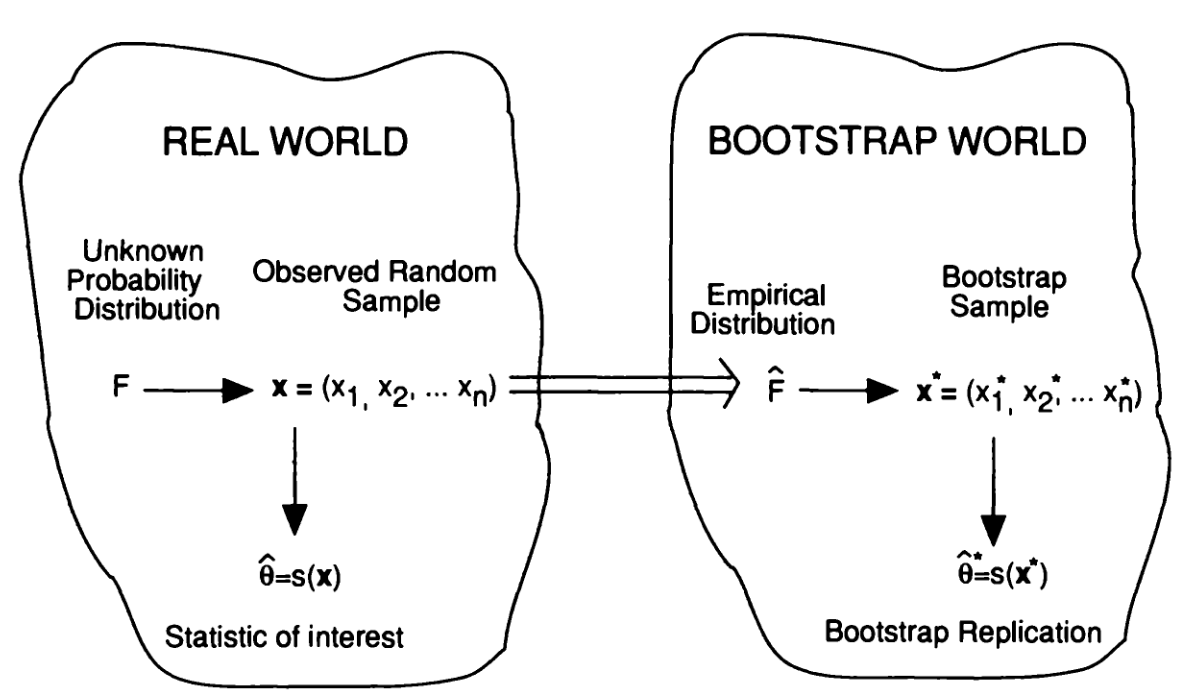
\includegraphics[width=0.88\textwidth]{figures/11-bootstrap-principle.png}
  \caption{Bootstrap 中总体、经验分布与重抽样经验分布的对应。图片来自 \cite{efrontibshirani1993}, p.~91}
  \label{fig:ch11:bootstrap-principle}
\end{figure}

Peter Hall 将此称作``俄罗斯套娃原则''，如图~\ref{fig:ch11:russian-doll-principle} 所示。

\begin{figure}[htbp]
  \centering
  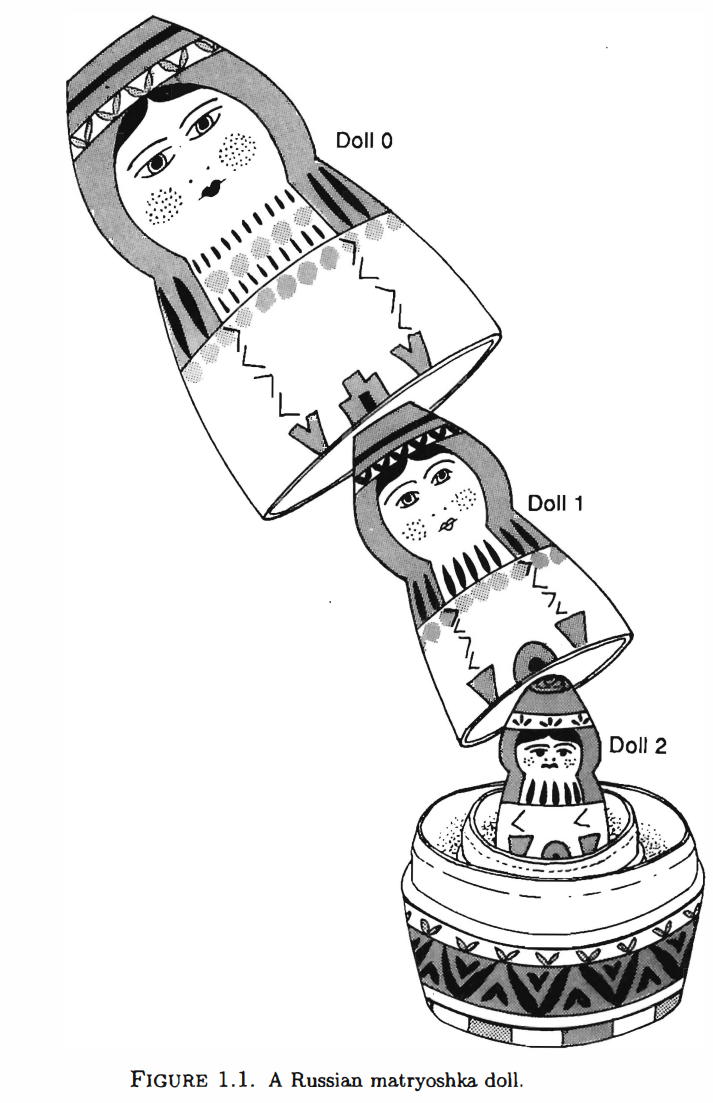
\includegraphics[height=0.68\textheight]{figures/11-russian-doll-principle.png}
  \caption{Bootstrap 的俄罗斯套娃原则。图片来自 \cite{hall1992}, p.~5}
  \label{fig:ch11:russian-doll-principle}
\end{figure}

基于上述原则，当我们想要模拟 $\sqrt{n}(\widehat{\theta}_n-\theta_0)$ 时，需要使用 $\sqrt n\big(\widehat{\theta}_n^*-\widehat{\theta}_n\big)$ 来进行刻画。

\begin{remark}

\begin{itemize}
\tightlist
\item
  理论上，如果统计量足够光滑，我们可能在上述算法基础上继续套一层，做``套娃的套娃''；但一般来讲这种做法意义不大，套一次就已足够。
\item
  上文中独立、有放回地重新抽取的样本 $X_1^*,\dots,X_n^*$ 数目仍然为 $n$ ，这里没有什么特别的原因，我们也可以非常自由地选择重抽样样本数：可以是某 $m$ ，也可以让 $m=m_n$ 随 $n$ 变化。但是 $m=n$ 是最常用的选择，对于我们后面要证明的结论也都足够。
\item
  注意到，理论中的 $P^*$ 是给定数据后的精确条件分布，而 Bootstrap 算法里是在用有限次重抽样近似它。记
  \[
  \widehat F_B^*(x)=\frac1B\sum_{b=1}^B
  \mathbb I(\widehat\theta_n^{*(b)}\leq x).
  \]
  则总误差可分解为
  \[
  \begin{aligned}
  \widehat F_B^*(x)-P(\widehat\theta_n\leq x)
  &=\left(\widehat F_B^*(x)-P^*(\widehat\theta_n^*\leq x)\right)\\
  &\quad+\left(P^*(\widehat\theta_n^*\leq x)-P(\widehat\theta_n\leq x)\right).
  \end{aligned}
  \]
  第一项是 Monte Carlo 误差，通常有 $B^{-1/2}$ 量级；第二项是 Bootstrap 方法本身的统计逼近误差。增加重复次数 $B$ 即可减少前者，因此在理论分析中，我们只关注 $P^*(\widehat\theta_n^*\leq x)-P(\theta_n\leq x)$ 这一项在 $n\to\infty$ 时的误差阶。如果能得到这项的阶，也可以帮助我们反过来确定 $B$ ，使得 Monte Carlo 误差与 Bootstrap 误差大概同阶。
\end{itemize}
\end{remark}

Bootstrap 是一个很直观很好用的办法，但是理论的建立并不容易，一般高阶刻画都比较难。我们接下来从一些更偏理论的角度，来对 Bootstrap 进行简单考察。

\subsection{条件弱收敛的补充}

本节补充部分``取条件版本''的若干概念和定理。这些细节主要用于保证在取条件时随机收敛概念严谨；读者可以略过，在后文中只需简单理解为``给定数据后的条件分布趋近于目标分布''即可。

\begin{definition*}[条件依概率收敛与条件弱收敛]
设 $Y_n$ 是样本空间 $(\Omega,\mathscr F,P)$ 中条件于给定 $\sigma$-代数 $\mathscr G_n$ 的一维统计量，后文 $\mathbb E[\ \cdot \mid \mathscr G_n]$、$P(\ \cdot\mid \mathscr G_n)$ 和条件独立等均视作某个正则条件分布的同一版本。

\begin{itemize}
\tightlist
\item
  \textbf{条件依概率收敛} 若 $Y$ 是定义于同一样本空间的随机变量，且对任意 $\epsilon>0$ ，都有 $P(|Y_n-Y|>\epsilon \mid \mathscr G_n)\overset{ P}\to 0$ ，则称 $Y_n\overset{P|\mathscr G_n}\to Y$ (依概率成立)。
\item
  \textbf{条件弱收敛} 若 $P(Y_n\le t\mid \mathscr G_n)\overset{P}\to P(Y\le t)$ ，对每个 $P(Y\le t)$ 的连续点 $t$ 成立，则称 $Y_n\overset{\rm d|\mathscr G_n}\to Y$ (依概率成立)。
\end{itemize}
\end{definition*}

\begin{remark}

\begin{itemize}
\tightlist
\item
  上面的全部 $\overset{P}\to 0$ 可以替换成 $\overset{\text{a.s.}}\to 0$ ，对应的结论替换为 a.s. 成立。
\item
  在更一般的情形，我们用\emph{有界 Lipschitz 度量}进行刻画条件弱收敛：设 $(M,d)$ 是某可分度量空间，\[ \mathrm{BL}_1(M):=\Big\{f:M\to\mathbb R:\sup_{z\in M}|f(z)|\le 1,\ |f(z_1)-f(z_2)|\le d(z_1,z_2),\ \forall z_1,z_2\in M\Big\} \]那么对 $M$ 上的两个 Borel 测度 $P,Q$ ，定义二者的有界 Lipschitz 度量为
  $$d_{\mathrm{BL}_1}(P,Q)=\sup_{f\in\mathrm{BL}_1(M)}\left|\int_Mf\mathrm dP-\int_M f\mathrm dQ\right|$$
  当一族概率测度 $\{P_n\}$ 满足 $d_{\mathrm{BL}_1}(P_n,P)\to 0$ 依概率/a.s. 收敛时，我们便称 $P_n\overset{\rm d}\to P$ 依概率/a.s. 成立。见 \cite[1.12 节]{vandervaartwellner1996}。% van de Vaart \emph{Weak Convergence and Empirical Processes} 的 1.12。
\end{itemize}
\end{remark}

此时也有若干``条件版本的定理''成立，我们本节只介绍其中一个：

\begin{theorem*}[条件 Lindeberg-Feller CLT]

对于每个 $n$，设 $\{Z_{n,j},j=1,\dots,k_n\}_{n\ge 0}$ 为在给定 $\sigma$-代数 $\mathscr{G}_n$ 的条件下的实值独立随机变量组列。假设
\[\mathbb{E}[Z_{n,j} \mid \mathscr{G}_n] = 0, \quad \mathrm{Var}[Z_{n,j} \mid \mathscr{G}_n] = \sigma_{n,j}^2 \in [0, \infty)\]
并记 $\sigma_n^2 := \sum_{j=1}^{k_n} \sigma_{n,j}^2$。如果对于某个 $\sigma^2 \in (0, \infty)$ 有 $\sigma_n^2 \overset{ P}\to \sigma^2$，并且对任意的 $\epsilon > 0$，有如下``条件 Lindeberg 条件''成立：
\[L_n(\epsilon) := \frac{1}{\sigma_n^2} \sum_{j=1}^{k_n} \mathbb{E}\left[ Z_{n,j}^2 \mathbb I(|Z_{n,j}| > \epsilon \sigma_n)\  \Big|\  \mathscr{G}_n \right] \overset P\to 0\]
那么
\[\sum_{j=1}^{k_n} Z_{n,j} \ \Big|\ \mathscr{G}_n \overset{\rm d}\to \mathcal{N}(0, \sigma^2)\]
依概率成立。

若定理中 $\sigma_n^2\overset P\to \sigma^2$ 和 $L_n(\epsilon)\overset{P}\to 0$ 均改成 a.s. 收敛，则最终结论 a.s. 成立。

\end{theorem*}

\begin{proof}[证明概要]

\begin{itemize}
\tightlist
\item
  先证明 a.s. 版本：存在一个概率为 1 的集合 $\Omega_0\subset \Omega$，使得对每个 $\omega\in \Omega_0$，$\sigma_n^2(\omega)\to\sigma^2$ 且 $L_n(\epsilon)(\omega)\to0$ 对所有 $\epsilon\in\mathbb Q_+$ 成立。这里只取正有理数，是为了避免不可数多个事件求交；由于 $L_n(\epsilon)$ 关于 $\epsilon$ 单调，上式实际上对所有 $\epsilon>0$ 成立。又因 $\sigma^2>0$，除有限项外都有 $\sigma_n^2(\omega)>0$。固定这样的 $\omega$ 后，可直接应用第~\ref{ch:central-limit-theorems}~章的 Lindeberg--Feller 中心极限定理~\ref{thm:ch3:lindeberg-feller}，得到
\end{itemize}
\[\begin{aligned} &P\left(\frac{1}{\sigma_n} \sum_{j=1}^{k_n} Z_{n,j} \le t\ \Bigg|\ \mathscr{G}_n \right)(\omega)\to \Phi(t)\\ \overset{\sigma_n^2(\omega)\to\sigma^2}\Longrightarrow\ & P\left(\frac{1}{\sigma} \sum_{j=1}^{k_n} Z_{n,j} \le t\ \Bigg|\ \mathscr{G}_n \right)(\omega)\to \Phi(t) \end{aligned}\]
对每个 $t\in\mathbb R$ 成立。 - ``依概率''版本需要绕一个弯子：我们知道依概率收敛于 0 当且仅当每个子列都存在进一步的子列 a.s. 收敛于 0 （例如，可见\cite{durrett2010} 的 Theorem 2.3.2）。 那么 $\sigma_n^2\overset P\to \sigma^2$ 和 $L_n(\epsilon)\overset{P}\to 0$ 蕴含：对每个子列 $\{n'\}$ 都存在进一步的子列 $\{n''\}$ 使得 \[ \sigma_{n''}^2\overset{\text{a.s.}}\to\sigma^2,\qquad L_{n''}(\epsilon)\overset{\text{a.s.}}\to0,\quad \forall \epsilon\in\mathbb Q_+ \]此时应用 a.s. 的情形的证明，再反过来用子列判别准则，给出 \[ P\left(\frac{1}{\sigma} \sum_{j=1}^{k_n} Z_{n,j} \le t\ \Bigg|\ \mathscr{G}_n \right)\overset P\to \Phi(t) \]对每个 $t\in\mathbb R$ 成立。

\end{proof}

\begin{remark}

\begin{itemize}
\tightlist
\item
  在无条件的意义下，这退化为经典 Lindeberg-Feller CLT： $\sum_{j=1}^{k_n} Z_{n,j} \overset{\rm d}\to \mathcal{N}(0, \sigma^2)$。
\item
  关于``条件中心极限定理''，可以参考 \cite{bulinski2016} 的 Theorem 1，作者给出了充要条件。
\item
  这种``子列论证 (subsequence argument)''的思路非常普遍，在 Bootstrap 的渐近分析中尤其多。读者可以尝试用这种方法证明条件版本的 Portmanteau 定理、连续映射定理、 Slutsky 定理和 Pólya 定理。 以条件版本的 Pólya 定理为例，简而言之：当 $Y$ 的分布函数处处连续时， $Y_n\overset{\rm d|\mathscr G_n}\to Y$依概率成立，当且仅当 
  $$\sup_x|P(Y_n\le x\mid \mathscr G_n)-P(Y\le x)|\overset P\to 0$$ 
  它正好是 Bootstrap``一阶正确''的形式。
\end{itemize}
\end{remark}

\subsection{均值的例子------一阶正确性}

这里以最简单的例子，均值为例，看下 Bootstrap 具体是如何起作用的。

设样本 $X_1,\dots,X_n\sim P$ i.i.d. ，总体有均值 $\mathbb E_P[X]=\mu$ 和 $\mathrm{Var}_P[X]=\sigma^2<\infty$ ，在上面的算法中取 $\theta(P)=\mathbb E_P[X]$ ，则``插入估计''就是样本均值 $\textstyle \bar{X}_n=\frac{1}{n}\sum_{j=1}^nX_j$ 。在重抽样后，Bootstrap 样本均值记作 $\textstyle \bar{X}_n^*=\frac{1}{n}\sum_{j=1}^nX_j^*$ 。

我们希望检验``套娃''了一层后的 $\sqrt{n}(\bar{X}_n^*-\bar{X}_n)$ 能否近似外层的 $\sqrt{n}(\bar{X}_n-\mu)$ 之分布。接下来记
\[\begin{aligned} P^*(\cdot)&:=P(\ \cdot\mid X_1,\dots,X_n)\\ \mathbb{E}^*[\cdot] &:= \mathbb{E}[\ \cdot\mid X_1,\dots,X_n] \\ \mathrm{Var}^*[\cdot] &:=\mathrm{Var}[\ \cdot\mid X_1,\dots,X_n] \end{aligned}\]
那么显然，至少在条件均值和条件方差的层面看，两层机制是相符的：
\[\mathbb{E}^*[X_j^*]=\bar{X}_n \implies \mathbb{E}^*[\bar{X}_n^*]=\bar{X}_n\]\[\begin{aligned} & \mathrm{Var}^*[X_j^*]=\mathbb E^*[(X_j^*-\bar{X})^2]=\frac{1}{n}\sum_{j=1}^n(X_j-\bar{X}_n)^2 =:S^2_n\\ \implies & \mathrm{Var}^*\!\left[\sqrt{n}(\bar{X}_n^*-\bar{X}_n)\right] =S^2_n \end{aligned}\]
由大数律， $S^2_n\overset{P}\to \sigma^2$ ，所以 Bootstrap 方差至少是正确收敛于真实方差的。

对 Bootstrap 样本均值，我们可以用上一节的条件 Lindeberg-Feller CLT 证明，``在原始样本下， $\sqrt{n}(\bar{X}_n^*-\bar{X}_n)$ 的条件分布收敛于正态分布 $\mathcal N(0,\sigma^2)$''，从而，Bootstrap 样本均值是一阶正确的。

下面记`` $\overset{\rm d^*}\to$ ''代表条件于样本下的弱收敛 (依概率成立)；`` $\overset{P^*}\to$ ''和`` $o_{P^*}(1)$ ''均代表条件于样本下的依概率收敛 (依概率成立)。

\begin{theorem}[Bootstrap 中心极限定理]
\label{thm:ch11:bootstrap-mean-clt}

对一维样本 $X_1,\ldots,X_n\sim P$ i.i.d.，总体有均值 $\mu\in\mathbb R$ 和方差 $0<\sigma^2<\infty$ ，则
\[\sqrt{n}(\bar{X}_n^*-\bar{X}_n) \mid X_1,\ldots,X_n \overset{\rm d^*}\to \mathcal{N}(0,\sigma^2)\]
\end{theorem}

\begin{proof}

考虑对
\[
\sqrt{n}(\bar{X}_n^*-\bar{X}_n) = \frac{1}{\sqrt{n}}\sum_{j=1}^n(X_j^*-\bar{X}_n).
\]
用条件 Lindeberg-Feller 中心极限定理。前文已经表明，条件于原始样本，上式有条件方差 $S^2_n$ 。往证``条件 Lindeberg 条件''成立，即：对任意 $\epsilon>0$ ，
\[L_n(\epsilon):=\frac{1}{S^2_n}\mathbb{E}^*\!\Big[ (X_1^*-\bar{X}_n)^2 \mathbb{I} \left( |X_1^*-\bar{X}_n|>\epsilon\sqrt{n}S_n \right) \Big] \overset{P}\to 0\]
由于 $S^2_n\overset{P}\to \sigma^2>0$ ，所以事件 $A_n:=\{S_n>\sigma/2\}$ 发生的概率趋于 1： $P(A_n)\to 1$ 。在 $A_n$ 上有
\[
\epsilon\sqrt{n}S_n\geq c\sqrt n, \qquad \frac{1}{S_n^2}\leq\frac{4}{\sigma^2}.
\]

其中常数 $c=\epsilon\sigma/2$ ，从而，
\[L_n(\varepsilon) \leq \frac 4{\sigma^2} \mathbb{E}^*\!\Big[ (X_1^*-\bar{X}_n)^2 \mathbb{I}(|X_1^*-\bar{X}_n|>c\sqrt{n}) \Big]\]
依概率成立。

现在只需再证明上式右侧的条件截断二阶矩依概率收敛到 0。记 $B_n=\{|\bar{X}_n-\mu|\leq c\sqrt n/2\}$ ，由于 $\bar X_n-\mu=O_P(n^{-1/2})$ ，有 $P(B_n)\to 1$ 。由三角不等式，
\[ B_n\cap \{|X_j-\bar X_n|>c\sqrt n\}\subset \big\{|X_j-\mu| \geq |X_j-\bar{X}_n|-|\bar{X}_n-\mu| > c\sqrt n/2\big\} \]那么在 $B_n$ 上便有：

\begin{equation}
\label{eq:ch11a:tag-1}
\begin{aligned} & \mathbb{E}^*\!\Big[ (X_1^*-\bar{X}_n)^2 \mathbb{I}(|X_1^*-\bar{X}_n|>c\sqrt{n}) \Big]\\ =\ &\frac{1}{n}\sum_{j=1}^n (X_j-\bar{X}_n)^2 \mathbb I(|X_j-\bar{X}_n|>c\sqrt{n})\\ \le\ & \frac{2}{n}\sum_{i=1}^n(X_i-\mu)^2\mathbb{I}\left(|X_i-\mu|>\frac{c\sqrt{n}}{2}\right)+2(\bar{X}_n-\mu)^2 \end{aligned}
\end{equation}

式~\eqref{eq:ch11a:tag-1} 的第二项由 $\bar X_n\overset{P}\to \mu$ 可知是 $o_P(1)$ 的；至于第一项，由控制收敛定理知其期望收敛到 0，从而由 Markov 不等式，该项也是 $o_P(1)$ 的；于是整个式~\eqref{eq:ch11a:tag-1} 都依概率收敛到 0。结合 $P(A_n\cap B_n)\to1$，即可得到 $L_n(\epsilon)\overset{P}\to0$。

由此结合 $S_n\overset{P}\to\sigma$ ，条件 Lindeberg-Feller 中心极限定理给出
\[
\sqrt n(\bar X_n^*-\bar X_n) \mid X_1,\ldots,X_n \overset{\rm d^*}\to \mathcal{N}(0,\sigma^2).
\]

\end{proof}

\begin{remark}

\begin{itemize}
\tightlist
\item
  实际上，我们也可以把定理~\ref{thm:ch11:bootstrap-mean-clt} 的结论直接加强到 a.s. 成立：只需要根据强大数律，对几乎所有的样本点都有 $\bar X_n\to\mu$ 和 $S_n^2\to\sigma^2$ 成立，所以 $n\to\infty$ 时 $A_n\cap B_n$ 是 a.s. 成立的；在该事件上，证明式~\eqref{eq:ch11a:tag-1} a.s. 收敛到 0 也是容易的。
\item
  关于定理~\ref{thm:ch11:bootstrap-mean-clt} 的相关参考：见 \cite{bickelfreedman1981} 的 Theorem 2.1，或者 \cite{vandervaart1998} 的 Theorem 23.4。
\item
  也可以用 Berry-Esseen 不等式来进行证明（\cite{singh1981}），例如可见 \href{https://zhuanlan.zhihu.com/p/2018774323612133216}{测度论与概率论 \textbar{} 17 自助法（The Bootstrap）}这里的定理17.1.1 。\cite{shaotu1996} 的 3.1 便总结了这两种不同方法。
\end{itemize}

\end{remark}

\begin{corollary}\label{cor:ch11:bootstrap-mean-uniform}
由条件版本的 Pólya 定理，定理~\ref{thm:ch11:bootstrap-mean-clt} 的结论表明
\[\sup_x \left| P^*\!\left(\sqrt{n}(\bar{X}_n^*-\bar{X}_n)\leq x\right) -\Phi(x/\sigma) \right| \overset{P}\to 0\]
从而
\[\sup_x \left| P^*\!\left(\sqrt{n}(\bar{X}_n^*-\bar{X}_n)\leq x\right) - P\!\left(\sqrt{n}(\bar{X}_n-\mu)\leq x\right) \right| \overset{P}\to 0\]\end{corollary}

\subsection{均值的例子------二阶准确性}

论证了一阶展开之后，我们来继续研究 Bootstrap 的高阶修正效果。先假设 $\sigma^2>0$ 已知，定义
\[Z_n:=\frac{\sqrt{n}(\bar{X}_n-\mu)}{\sigma},\quad Z_n^*:=\frac{\sqrt n(\bar X_n^*-\bar X_n)}{\sigma}\]
若 $\mathbb{E}[|X|^4]<\infty$，并且 $X$ 的特征函数满足 Cramér 条件，则对 $Z_n$ 用 Edgeworth 展开：
\[P(Z_n\leq x) = \Phi(x) -\frac{\gamma_1}{6\sqrt{n}}(x^2-1)\varphi(x) +O(n^{-1})\]
其中 $\gamma_1:=\frac{\mathbb{E}[(X-\mu)^3]}{\sigma^3}$ 代表总体偏度；这一形式已在第~\ref{ch:characteristic-functions}~章推导，它表明正态近似的第一个修正项与总体偏度成正比。

Bootstrap 估计会对使用插入估计近似 Edgeworth 展开的项，具体而言， $\gamma_1$ 会变成下述经验偏度
\[\widehat{\gamma}_{1,n}=\frac{n^{-1}\sum_{i=1}^n(X_i-\bar{X}_n)^3}{\left(n^{-1}\sum_{i=1}^n(X_i-\bar{X}_n)^2\right)^{3/2}}\]
只要能保证 $\widehat\gamma_{1,n}-\gamma_1=O_P(n^{-1/2})$ ，那么一阶修正项的匹配误差就是 $n^{-1/2}\times O_{P}(n^{-1/2})=O_{P}(n^{-1})$。Bootstrap 就满足了二阶准确性。

那么，经验偏度的估计效率是否能满足我们的要求呢？当然了，有下面的结论：

\begin{lemma*}

记 $a_{r,n}$ 代表 $r$ 阶样本原点矩、 $\alpha_r=\mathbb E[X^r]$ 代表 $r$ 阶总体原点矩，光滑函数 $H:\mathbb R^r\to\mathbb R$ 在 $(\alpha_1,\dots,\alpha_r)^\top$ 处的梯度非 0。记 $\theta=H(\alpha_1,\dots,\alpha_r)$ 、 $\widehat\theta_n:=H(a_{1,n},\dots,a_{r,n})$ ，那么当 $\mathbb E[X^{2r}]<\infty$ 时， $\widehat\theta_n$ 满足渐近正态性
\[
\sqrt n(\widehat\theta_n-\theta)\overset{\rm d}\to\mathcal N(0,\sigma^2).
\]

\end{lemma*}

\begin{proof}

对 $f(X)=(X,\dots, X^r)^\top$ 和真实参数 $(\alpha_1,\dots,\alpha_r)^\top$ 使用第~\ref{ch:method-of-moments}~章定理~\ref{thm:ch6:mom-asymptotic-normality} 的矩估计渐近正态性：
\[\sqrt n\left(\frac1n\sum_{j=1}^nf(X_j)-(\alpha_1,\dots,\alpha_r)^\top\right)=\sqrt n\left(a_{1,n}-\alpha_1,\dots,a_{r,n}-\alpha_r\right)^\top\overset{\rm d}\to \mathcal N(0,\Sigma_f)\]
这里 $\Sigma_f=(\alpha_{i+j}-\alpha_i\alpha_j)_{r\times r}$ 。对 $H$ 用 Delta 方法，即可得到
\[
\sqrt n(\widehat \theta_n-\theta)\overset{\rm d}\to \mathcal N\Big(\bm 0,(\nabla H(\alpha_1,\dots,\alpha_r))^\top \Sigma_f \nabla H(\alpha_1,\dots,\alpha_r)\Big).
\]

\end{proof}

\begin{corollary*}

\begin{itemize}
\tightlist
\item
  容易验证经验偏度 $\widehat \gamma_{1,n}$ 和总体偏度 $\gamma_1$ 可以表示为
  \[
  H(a_{1,n},a_{2,n},a_{3,n})=\widehat\gamma_{1,n},\qquad
  H(\alpha_1,\alpha_2,\alpha_3)=\gamma_1,
  \]
  其中
  \[
  H(a,b,c)=\frac{c-3ab+2a^3}{(b-a^2)^{3/2}}.
  \]
  那么 $\mathbb E[X^6]<\infty$ 时，
  \[
  \sqrt n(\widehat \gamma_{1,n}-\gamma_1)
  \overset{\rm d}\longrightarrow\mathcal N(0,\sigma_1^2),
  \]
  这便给出了 $\widehat \gamma_{1,n}-\gamma_1=O_P(n^{-1/2})$。
\item
  使用完全相同的方法，可以证明：当 $\mathbb E[X^8]<\infty$ 时，经验峰度 $\textstyle\widehat \gamma_{2,n}:=\frac{ n^{-1}\sum_{i=1}^n (X_i-\bar{X}_n)^4 }{ \left( n^{-1}\sum_{i=1}^n (X_i-\bar{X}_n)^2 \right)^2 } - 3$ 也是总体峰度 $\textstyle\gamma_2=\frac{\mathbb E[(X-\mu)^4]}{(\mathbb E[(X-\mu)^2])^2}-3$ 的渐近正态估计： $\sqrt n(\widehat \gamma_{2,n}-\gamma_2)\to\mathcal N(0,\sigma_2^2)$ 。
\item
  这两个渐近方差的具体形式也是可以算出来的。记
  $\mu_r=\mathbb E[(X-\mu)^r]$。经验偏度对应函数
  $g_1(u,v)=v/u^{3/2}$，其在 $(\mu_2,\mu_3)$ 处的梯度为
  \[
  \nabla g_1=
  \begin{pmatrix}
  -\dfrac{3\mu_3}{2\mu_2^{5/2}}\\[4pt]
  \dfrac1{\mu_2^{3/2}}
  \end{pmatrix}.
  \]
  样本二阶、三阶中心矩的渐近协方差矩阵为
  \[
  \Sigma_{2,3}=
  \begin{pmatrix}
  \mu_4-\mu_2^2 & \mu_5-4\mu_2\mu_3\\
  \mu_5-4\mu_2\mu_3 &
  \mu_6-\mu_3^2-6\mu_2\mu_4+9\mu_2^3
  \end{pmatrix}.
  \]
  因此
  \[
  \begin{aligned}
  \sigma_1^2
  &=\nabla g_1^{\top}\Sigma_{2,3}\nabla g_1\\
  &=\frac{9\mu_3^2(\mu_4-\mu_2^2)}{4\mu_2^5}
   -\frac{3\mu_3(\mu_5-4\mu_2\mu_3)}{\mu_2^4}
   +\frac{\mu_6-\mu_3^2-6\mu_2\mu_4+9\mu_2^3}{\mu_2^3}.
  \end{aligned}
  \]
  类似地，经验峰度对应函数 $g_2(u,v)=v/u^2-3$，且
  \[
  \nabla g_2=
  \begin{pmatrix}
  -\dfrac{2\mu_4}{\mu_2^3}\\[4pt]
  \dfrac1{\mu_2^2}
  \end{pmatrix},\qquad
  \Sigma_{2,4}=
  \begin{pmatrix}
  \mu_4-\mu_2^2 & \mu_6-\mu_2\mu_4-4\mu_3^2\\
  \mu_6-\mu_2\mu_4-4\mu_3^2 &
  \mu_8-\mu_4^2-8\mu_3\mu_5+16\mu_2\mu_3^2
  \end{pmatrix}.
  \]
  从而
  \[
  \begin{aligned}
  \sigma_2^2
  &=\nabla g_2^{\top}\Sigma_{2,4}\nabla g_2\\
  &=\frac{4\mu_4^2(\mu_4-\mu_2^2)}{\mu_2^6}
   -\frac{4\mu_4(\mu_6-\mu_2\mu_4-4\mu_3^2)}{\mu_2^5}\\
  &\qquad
   +\frac{\mu_8-\mu_4^2-8\mu_3\mu_5+16\mu_2\mu_3^2}{\mu_2^4}.
  \end{aligned}
  \]
  特别地，对正态分布有 $\sigma_1^2=6$、$\sigma_2^2=24$。
\end{itemize}
\end{corollary*}

当 $\sigma^2$ 未知时，上述 $Z_n$ 不能直接用于实际推断，为此，考虑标准化或称``学生化''统计量：
\[T_n=\frac{\sqrt{n}(\bar{X}_n-\mu)}{S_n},\qquad T_n^*=\frac{\sqrt{n}(\bar{X}_n^*-\bar{X}_n)}{S_n^*}\]
其中
\[
S^2_n:=\frac1n\sum_{j=1}^n(X_j-\bar X_n)^2,\quad {S_n^*}^2= \frac1n\sum_{j=1}^n(X_j^*-\bar{X}_n^*)^2.
\]

``学生化''还有一个重要作用是，除以 $S_n$ 相对于自适应地调整了尺度，使得 $T_n$ 成为渐近枢轴量，从而，其渐近特性可以直接通过 Edgeworth 展开来表示。这也可称作``自归一化 (Self-Normalization)''，例如 \cite{delapena2009} 一书的 Chapter 16 所述。

我们还没有计算过 $T_n$ 的 Edgeworth 展开，这里简单推导一下。（不想看细节的读者可以下滑到式~\eqref{eq:ch11a:tag-3} :-）

总的思路是从 $S_n$ 下手。记
\[
Y_j:=\frac{X_j-\mu}{\sigma},\qquad V_n:=\frac1{\sqrt n}\sum_{j=1}^n(Y_j^2-1).
\]

将 $S_n^2$ 写作
\[\begin{aligned} S_n^2 &=\sigma^2\left(\frac1n\sum_{i=1}^n Y_i^2-\left(\frac1n\sum_{i=1}^n Y_i\right)^2\right) \\ &=\sigma^2\left(1+\frac{1}{\sqrt n}\left(\frac1{\sqrt n}\sum_{i=1}^n(Y_i^2-1)\right)-\frac1n\left(\frac1{\sqrt n}\sum_{i=1}^n Y_i\right)^2\right) \\ &=\sigma^2\left(1+\frac{V_n}{\sqrt n}-O_P(n^{-1})\right) \\  \end{aligned}\]
利用 $(1+x)^{-1/2}=1-\frac12 x+O(x^2)$ 可得
\[\begin{aligned} T_n&=Z_n\frac{\sigma}{S_n}=Z_n-\frac{1}{2\sqrt n}Z_nV_n+O_P(n^{-1})\\  \end{aligned}\]
这里的第二项 $-\frac1{2\sqrt n}Z_nV_n$ 衡量了 $T_n$ 与 $Z_n$ 两个量之间的 $n^{-1/2}$ 阶差距；这导致特征函数有
\[\begin{aligned} \phi_{T_n}(t)&=\mathbb E\left[\exp\left\{it Z_n-\frac{it}{2\sqrt n}Z_nV_n+O_P(n^{-1})\right\}\right]\\ &=\mathbb E\left[e^{itZ_n}\left(1-\frac{it}{2\sqrt n}Z_nV_n+O_P(n^{-1})\right)\right]\\ &=\phi_{Z_n}(t)-\frac{it}{2\sqrt n}\mathbb E[Z_nV_n e^{itZ_n}]+o(n^{-1/2}) \end{aligned}\]
对 $n\to\infty$ 取极限后，

\begin{itemize}
\tightlist
\item
  第一项可以用第~\ref{ch:characteristic-functions}~章介绍的 $\phi_{Z_n}(t)$ 渐近展开：$\phi_{Z_n}(t)=e^{-t^2/2}\left(1+\frac{1}{6\sqrt n}\gamma_1(it)^3+o(n^{-1/2})\right)$。
\item
  记 $(Z_n,V_n)\overset{\rm d}\to (Z,V)$ ，极限分布是一个二维正态分布，且 $Z$ 的边际分布是 $\mathcal N(0,1)$；那么第二项有
  \[
  \begin{aligned}
  \mathbb E[Z_nV_n e^{itZ_n}]
  &\to \mathbb E[ZV e^{itZ}]\\
  &=\mathbb E\Big[Ze^{itZ}\underbrace{\mathbb E[V|Z]}_{\gamma_1Z}\Big]\\
  &=\gamma_1\mathbb E[Z^2e^{itZ}]
  =\gamma_1(1-t^2)e^{-t^2/2}.
  \end{aligned}
  \]
  最后一步来自
  \[
  \mathbb E[Z^2e^{itZ}]
  =-\phi''_Z(t)=(e^{-t^2/2})''=(1-t^2)e^{-t^2/2}.
  \]
\item
  综上， $\phi_{T_n}(t)$ 的渐近展开为
  \[  \begin{aligned} \phi_{T_n}(t)&=e^{-t^2/2}\left(1+\frac{1}{6\sqrt n}\gamma_1(it)^3-\frac1{2\sqrt n}\gamma_1 it(1-t^2)+o(n^{-1/2})\right)\\ &=e^{-t^2/2}\left(1+\frac{1}{\sqrt n}\left(-\frac{\gamma_1}{3}(it)^3-\frac{\gamma_1}2it\right)+o(n^{-1/2})\right). \end{aligned}
  \]\end{itemize}

记多项式 $r_1(u)=-\tfrac{\gamma_1}{3}u^3-\tfrac {\gamma_1}2 u$ ，那么 $\phi_{T_n}(t)=e^{-t^2/2}(1+n^{-1/2}r_1(it)+o(n^{-1/2}))$ ，进行特征函数的反演后， $T_n$ 的 Edgeworth 展开第一项应为
\[r_1(-D)\Phi(x)=\frac{\gamma_1}{2}\varphi(x)+\frac{\gamma_1}{3}(x^2-1)\varphi(x)  =\frac{\gamma_1}{6}(1+2x^2)\varphi(x)\]
综上，学生化统计量 $T_n=\frac{\sqrt n(\bar X-\mu)}{S_n}$ 的 Edgeworth 展开为

\begin{equation}
\label{eq:ch11a:tag-3}
P(T_n\leq x) = \Phi(x) +\frac{\gamma_1}{6\sqrt{n}}(1+2x^2)\varphi(x) +O(n^{-1})
\end{equation}

在 $\mathbb E[X^6]<\infty$ 时候，仍然有 $\widehat\gamma_{1,n}-\gamma_1=O_P(n^{-1/2})$ ，所以 Bootstrap 统计量 $T_n^*$ 是二阶准确的。

我们将本节的分析总结成下面的定理：

\begin{theorem}[Bootstrap 的二阶准确性]\label{thm:ch11:second-order-accuracy}

设 $\mathbb E[X^6]<\infty$ 且 Cramér 条件 $\limsup\limits_{|t|\to\infty}|\phi_X(t)|<1$ 成立，那么
\[P^*(Z_n^*\le x)=P^*\left(\frac{\sqrt n(\bar X_n^*-\bar X_n)}{\sigma}\le x\right)=\Phi(x)+\frac{\widehat\gamma_{1,n}}{6\sqrt n}(1-x^2)\varphi(x)+O(n^{-1})\]
并且

\[
\sup_x \left| P^*(Z_n^*\leq x)-P(Z_n\leq x) \right| =O_P(n^{-1}).
\]
若以趋近于 1 的概率有 $S^2_n>0$ 、 ${S_n^*}^2>0$ ，那么
\[
P^*(T_n^*\le x)=P^*\left(\frac{\sqrt n(\bar X^*_n-\bar X_n)}{S^*_n}\le x\right)=\Phi(x)+\frac{\widehat\gamma_{1,n}}{6\sqrt n}(1+2x^2)\varphi(x)+O(n^{-1}).
\]

并且

\[
\sup_x \left| P^*(T_n^*\leq x)-P(T_n\leq x) \right| =O_P(n^{-1}).
\]

\end{theorem}
我们成功表明：通过自动估计 Edgeworth 一阶校正项，Bootstrap 实现了二阶准确！

当 $X$ 有更高的矩条件，我们能够将 Edgeworth 展开到更高阶项，从而得到更精确的近似。例如，当 $\mathbb E[X^8]<\infty$ 时，有
\[\begin{aligned} P(Z_n\le x) &= \Phi(x) + \frac{\gamma_1}{6\sqrt{n}}(1-x^2)\varphi(x) - \frac{3\gamma_2(x^3-3x)+\gamma_1^2(x^5-10x^3+15x)}{72n}\,\varphi(x) + O\!\left(n^{-3/2}\right)\\  P(T_n\le x)&= \Phi(x) + \frac{\gamma_1(1+2x^2)}{6\sqrt{n}}\varphi(x) + \frac{3\gamma_2(x^3-3x)-2\gamma_1^2(x^5+2x^3-3x)-9(x^3+3x)}{36n}\,\varphi(x) + O\!\left(n^{-3/2}\right) \end{aligned}\]
（例如，见 \cite{hall1992}, pp.~71--73。）

但是，受限于 $\widehat\gamma_{1,n}-\gamma_1=O_P(n^{-1/2})$ 的误差，即使展开到高阶项，仍然是第一项占主导，我们也只能得到 $O(n^{-1})$ 。

\subsection{推广到非线性光滑泛函}

均值 $\theta(P)=\mathbb E_P[X]$ 是一个线性统计泛函。所谓``线性统计泛函''指的是一切形如 
$$P\mapsto \int h(x)\mathrm dP(x)$$
的统计泛函，其中 $h$ 满足 $\textstyle\int|h(x)|\mathrm dP(x)<\infty$ 。利用 $\mathbb P_n$ 近似 $P$ ------或者说，插入估计
\[\int h(x)\mathrm d\mathbb P_n(x)=\frac1n\sum_{j=1}^nh(X_j)\overset{P}\to \int h(x)\mathrm{d}P(x)=\mathbb E_P[h(X)]\]
本质上还是 $Y=h(X)$ 的样本均值近似总体均值，可以照搬前面均值情形 Bootstrap 的结论。

要将结论推广到非线性的 $\theta(P)$ ，需要用到线性化的思想，这和一阶 Taylor 展开如出一辙。简单起见，我们只考虑一维情形，推广到高维是直接的。

\begin{definition*}[Gâteaux 导数与影响函数]
设 $P,Q$ 是两个 $\mathbb R$ 上的概率测度，定义统计泛函 $\theta$ 在 $P$ 沿 $Q$ 方向的 \textbf{\emph{Gâteaux 导数}} 为
\[\theta'_P(Q):=\lim_{\epsilon\downarrow 0}\frac{\theta((1-\epsilon)P+\epsilon Q)-\theta(P)}{\epsilon}\]
特别地，若取 $Q=\delta_x$ 是 $x$ 处的点概率，那么记 $\mathrm{IF}_P(x)=\theta'_P(\delta_x)$ ：
\[
\mathrm{IF}_P(x):=\lim_{\epsilon\downarrow 0}\frac{\theta((1-\epsilon)P+\epsilon \delta_x)-\theta(P)}{\epsilon}.
\]

并称 $\mathrm{IF}_P(x)$ 为\textbf{\emph{影响函数}} (influence function)。将上式的 $P$ 替换为 $\mathbb P_n$ ，得到
\[
\widehat{\mathrm{IF}}_n(x)=\lim_{\epsilon\downarrow 0}\frac{\theta((1-\epsilon)\mathbb P_n+\epsilon \delta_x)-\theta(\mathbb P_n)}{\epsilon}.
\]

称作\textbf{\emph{经验影响函数}} 。
\end{definition*}

\begin{remark}
设 $X_1,\dots,X_n\sim P$ i.i.d.，那么

\begin{itemize}
\tightlist
\item
  由 $\theta'_P$ 的线性性，可以得出影响函数期望为 0： \[ \mathbb E_P[\mathrm{IF}_P(X)]=\int \theta'_P(\delta_x-P)\mathrm{d}P(x)= \theta'_P\left(\int (\delta_x-P)\mathrm{d}P(x)\right)=\theta'_P(P-P)=0 \]这里的`` $\textstyle\int(\delta_x-P)\mathrm dP(x)$ ''视作测度 $A\mapsto \int(\delta_x(A)-P(A))\mathrm dP(x)$ ，其中 $A$ 是任意 Borel 可测集；由于 $\int(\delta_x(A)-P(A))\mathrm dP(x)=\int_A \mathrm{d}P(x)-P(A)=0$ ，所以这个积分是 0。
\item
  由中心极限定理， $\frac1{\sqrt n}\sum_{j=1}^n\mathrm{IF}_P(X_j)\overset{\rm d}\to \mathcal N(0,\mathrm{Var}[\mathrm{IF}_P(X)])$ ；我们后面会看到，一个满足适当正则条件的估计量，其渐近正态性质往往就是由影响函数贡献的，从而， $\mathrm{IF}_P$ 可以视作衡量了单个样本对渐近分布造成的``影响''。
\end{itemize}
\end{remark}

记 $D:=Q-P$ ，这是一个总质量为 0 的符号测度，那么 $\theta((1-\epsilon) P+\epsilon Q)=\theta(P+\epsilon D)$ ，也可以用 $D$ 来定义 Gâteaux 导数：
\[\lim_{\epsilon\downarrow 0}\left\|\frac{\theta(P+\epsilon D)-\theta(P)}{\epsilon}-\theta'_P(D)\right\|=0\]
即， $\theta(P+\epsilon D)=\theta(P)+\epsilon \theta'_P(D)+o(\epsilon)$ 。

在全体一维概率测度生成的向量空间（即，实数轴上的全体有限符号测度空间） $\mathscr D$ 上赋予 Kolmogorov 度量
\[
d_{\text{K}}(P,Q)=\sup_{x\in\mathbb R}|P(X\le x)-Q(X\le x)|.
\]

生成的拓扑，我们引入 Hadamard 可微性，其出发点是让 $o(\epsilon)$ 项一致地小。

\begin{definition*}[Hadamard 可微性]

\begin{itemize}
\tightlist
\item
  若对任意 $\epsilon_n\downarrow 0$ 以及总质量为 0 的 $D,D_1,D_2,\dots\in\mathscr D$使得 $d_{\text{K}}(D_n,D)\to 0$ ，存在线性泛函 $\theta'_P:\mathscr D\to \mathbb R$ 满足\[ \lim_{n\to\infty}\left\|\frac{\theta(P+\epsilon _nD_n)-\theta(P)}{\epsilon_n}-\theta'_P(D)\right\|=0 \]那么称 $\theta$ 在 $P$处（对 Kolmogorov 距离 $d_{\text{K}}$ ）是 \textbf{\emph{Hadamard 可微}} 的。
\item
  上述定义里要求``所有方向都一致收敛''，这个要求有时候会太强；因此，也可以把方向限制在某个 $\mathscr D_0\subset \mathscr D$ 中： 若对任意 $\epsilon_n\downarrow 0$ 以及总质量为 0 的 $D_1,D_2,\dots\in D_0$使得 $d_{\text{K}}(D_n,D)\to 0$ ，存在线性泛函 $\theta'_P:\mathscr D_0\to \mathbb R$ 满足\[ \lim_{n\to\infty}\left\|\frac{\theta(P+\epsilon _nD_n)-\theta(P)}{\epsilon_n}-\theta'_P(D)\right\|=0 \]那么称 $\theta$ 在 $P$处切于 $\mathscr D_0$ 是 Hadamard 可微的。
\end{itemize}

（上述定义亦可见 \cite{wasserman2006} 一书的 2.3，或者 \cite{shaotu1996} 的 2.2.1。）
\end{definition*}

\begin{theorem}[泛函 Delta 方法]
\label{thm:ch11:functional-delta-method}

设统计泛函 $\theta(P)$ 关于 Kolmogorov 度量 $d_{\text{K}}$ 在 $P$ 处切于 $\mathscr D_0\subset\mathscr D$ 是 Hadamard 可微的，导数为 $\theta'_P:\mathscr D\to \mathbb R$ ； $\{P_n\} \subset\mathscr D$ 满足： $a_n(P_n-P)\overset{\rm d}\to G$ ，其中随机元 $G$ 取值于 $\mathscr D_0$ 、 $a_n\to\infty$ ，那么
\[a_n(\theta(P_n)-\theta(P))\overset{\rm d}\to \theta'_P(G)\]
若 $\theta'_P$ 能延拓到整个 $\mathscr D$ 上（有定义且线性连续），则
\[a_n(\theta(P_n)-\theta(P))=\theta'_P(a_n(P_n-P))+o_P(1)\]
\end{theorem}

\begin{proof}[证明概要]
考虑映射
\[f_n(D)=a_n\left(\theta\left(P+\frac1{a_n}D\right)-\theta\left(P\right)\right)\]
Hadamard 可微性告诉我们，对任意 $D\in\mathscr D_0$ 和序列 $\{D_n\}\subset\mathscr D$ 满足 $d_{\text{K}}(D_n,D)\to 0$ 有 $f_n(D_n)\to \theta'_P(D)$ 。从而连续映射定理取给出 $f_n(a_n (P_n-P))\overset{\rm d}\to \theta_P'(G)$ 。

定理中的第二个式子来自对 $D\mapsto (\theta(D),\theta_P'(D))$ 用同样的论证。

\end{proof}

\begin{remark}
定理~\ref{thm:ch11:functional-delta-method} 详见 Van de Vaart, \emph{Asymptotic Statistics} 的 Theorem 20.8。
\end{remark}

它的一个推论如下：

\begin{corollary}\label{cor:ch11:functional-delta-normality}
对 $P$ 处 Hadamard 可微的泛函 $\theta$，设其影响函数满足 $0<\tau^2:=\mathbb E_P[\mathrm{IF}_P(X)^2]<\infty$，则
\[\sqrt n(\theta(\mathbb P_n)-\theta(P))\overset{\rm d}\to \mathcal N(0,\tau^2)\]
此外，若记 $\widehat{\tau}^2=\frac1n\sum_{j=1}^n\big(\widehat{\mathrm{IF}}_n(X_j)\big)^2$，那么
\[
\sqrt n\frac{\theta(\mathbb P_n)-\theta(P)}{\widehat\tau}
\overset{\rm d}\longrightarrow\mathcal N(0,1).
\]
\end{corollary}

\begin{proof}

根据泛函 Delta 方法，
\[\begin{aligned} \sqrt n(\theta(\mathbb P_n)-\theta(P))&=\theta'_P(\sqrt n(\mathbb P_n-P))+o_P(1)\\ &=\frac1{\sqrt n}\sum_{j=1}^n\underbrace{\theta'_P(\delta_{X_j}-P)}_{\mathrm{IF}_P(X_j)}+o_P(1)\\  &=\frac1{\sqrt n}\sum_{j=1}^n\mathrm{IF}_P(X_j)+o_P(1)\\ &\overset{\rm d}\to\mathcal N(0,\mathrm{Var}_P[\mathrm{IF}_P(X)])\\ &=\mathcal N(0,\tau^2) \end{aligned}\]
由大数律， $\widehat{\tau}^2\overset{P}\to \tau$ ，因此 Slutsky 定理给出 $\sqrt n\frac{\theta(\mathbb {P}_n)-\theta(P)}{\widehat\tau}\overset{\rm d}\to \mathcal N(0,1)$ 。

\end{proof}

\begin{remark}
也可以从经验过程的角度出发研究前面的讨论------因为 Bootstrap 一开始的想法：用经验分布逼近真实分布，本身就是个经验过程的概念。给定一族可测函数 $\mathscr F$，将 $\mathbb R$ 上的有限测度/符号测度视作作用于 $\mathscr F$ 的线性泛函：
\[P\mapsto Pf= \int_{\mathbb R}f\mathrm dP\in\ell^\infty(\mathscr F),\quad f\in\mathscr F\]
并赋予上确界范数 $\|P\|_{\mathscr F}=\sup_{f\in\mathscr F}\|Pf\|$ ；前面的 Kolmogorov 度量在这里对应取 $\mathscr F=\{x\mapsto \mathbb I(x\le t):t\in\mathbb R\}$ 时得到的上确界范数。当 $\mathscr F$ 是 Donsker 类时，经验过程在 $\ell^\infty(\mathscr F)$ 中弱收敛到 $P$ -Brown 桥： $\sqrt n(\mathbb P_n-P)\overset{\rm d}\to \mathbb G_P$ ，所以泛函 Delta 方法给出
\[\sqrt n(\theta(\mathbb P_n)-\theta(P))\overset{\rm d}\to \theta'_P(\mathbb G_P)\]
在推论~\ref{cor:ch11:functional-delta-normality} 的条件下，记 $\widehat\theta_n=\theta(\mathbb P_n)$ 为插入估计， $\theta_0=\theta(P)$ ，
\[\sqrt n(\widehat\theta_n-\theta_0)=\frac1{\sqrt n}\sum_{j=1}^n\mathrm{IF}_P(X_j)+o_P(1)\]
到这一步，我们已经成功将一个非线性的泛函给线性化了。
\end{remark}

用 Bootstrap 套一层娃，
\[\begin{aligned} \sqrt n(\widehat\theta_n^*-\widehat\theta_n)&=\theta'_P(\sqrt n(\mathbb P_n^*-\mathbb P_n))+o_{P^*}(1)\\ &=\frac1{\sqrt n}\sum_{j=1}^n(\mathrm{IF}_P(X_j^*)-\mathbb P_n\mathrm{IF}_P)+o_{P^*}(1)\\  &=\sqrt n\big(\mathbb P_n^*\mathrm{IF}_P-\mathbb P_n \mathrm{IF}_P\big)+o_{P^*}(1)\\ \end{aligned}\]
可以看出，这种情况下，Bootstrap 重新模拟的是影响函数的波动 。由定理~\ref{thm:ch11:bootstrap-mean-clt}（用 $\mathbb P_n^*\mathrm{IF}_P$ 替换 $\bar X_n^*$ 、用 $\mathbb P_n\mathrm{IF}_P$ 替换 $\bar X_n$ ）：
\[ \sqrt{n}(\mathbb P_n^*\mathrm{IF}_P-\mathbb P_n \mathrm{IF}_P) \mid X_1,\ldots,X_n \overset{\rm d^*}\to \mathcal{N}(0,\tau^2) \]其中 $\tau^2=\mathrm{Var}_P[\mathrm{IF}_P(X)]=\mathbb{E}_P[\mathrm{IF}_P(X)^2]$ ；从而，Bootstrap 估计量是一阶正确的。我们整理成下述定理：

\begin{theorem}[光滑统计泛函的 Bootstrap 一阶正确性]
\label{thm:ch11:bootstrap-smooth-functional}

设统计泛函 $\theta(P)$ 在 $P$ 处关于 Kolmogorov 距离 $d_{\text{K}}$ 是 Hadamard 可微的，并且影响函数满足 $0<\tau^2:=\mathbb E_P[\mathrm{IF}_P(X)^2]<\infty$ ，那么对 i.i.d. 样本 $X_1,\dots,X_n\sim P$ ，
\[\sqrt n(\theta(\mathbb P_n^*)-\theta(\mathbb P_n))\mid X_1,\dots,X_n\overset{\rm d^*}\to\mathcal N(0,\tau^2)\]
由此得出
\[\sup_x \Big| P^*\!\left(\sqrt{n}(\theta(\mathbb P_n^*)-\theta(\mathbb P_n))\leq x\right) -\Phi(x/\tau) \Big| \overset{P}\to 0\]
和
\[\sup_x \Big| P^*\!\left(\sqrt{n}(\theta(\mathbb P_n^*)-\theta(\mathbb P_n))\leq x\right) - P\!\left(\sqrt{n}(\theta(\mathbb P_n)-\theta(P))\leq x\right) \Big| \overset{P}\to 0\]
\end{theorem}

\begin{remark}
若统计泛函 $\theta(P)$ 在 $P$ 处关于 $d_{\text{K}}$ 切于某子空间 $\mathscr D_0$ 是 Hadamard 可微的，且 $\mathscr D_0$ 包含 $\mathbb G_P$，那么定理~\ref{thm:ch11:bootstrap-smooth-functional} 的结论仍然成立。
\end{remark}

定理~\ref{thm:ch11:bootstrap-smooth-functional} 只证明了一阶的正确。要解释高阶准确性，还要保留偏差和二次曲率项，形式上大概会像
\[
\widehat{\theta}_n-\theta_0=\frac{1}{n}\sum_{i=1}^n\mathrm{IF}_P(X_i)+\frac{1}{n}b(P)+Q_n(P)+o_{P}(n^{-1}).
\]

其中 $b(P)$ 是偏差项，$Q_n(P)$ 是包含经验过程的二次型的项，这里的系数均依赖未知 $P$。Bootstrap 估计就是把上述 $P$ 替换为 $\mathbb{P}_n$，因而能够自动估计偏差和曲率修正。

最后简单举两个具体例子。

\begin{example}[方差]\label{ex:ch11:variance}

设总体四阶矩存在，
\[\theta_0=\mathrm{Var}_P[X]=P(x^2)-(Px)^2\]
插入估计为
\[\widehat{\theta}_n=\mathbb{P}_nx^2-(\mathbb{P}_nx)^2\]
Bootstrap 估计量为
\[\widehat{\theta}_n^*=\mathbb{P}_n^*x^2-(\mathbb{P}_n^*x)^2\]
记 $\mu=Px$ 为均值，可以计算方差泛函的在 $D$ 方向的导数： $\theta'_P(D)=D (x^2) -2\mu D (x)=\int_{\mathbb R}(y^2-2\mu y)\mathrm dD(y)$ 特别地，取 $D=\delta_x-P$ ，得到影响函数 \[ \begin{aligned} \mathrm{IF}_P(x)&=\int_{\mathbb R}(y^2-2\mu y)\mathrm d(\delta_x-P)(y)\\ &=x^2-2\mu x-\mathbb E_P[X^2]+2\mu\mathbb E_P[X]\\ &=(x-\mu)^2-\sigma^2 \end{aligned} \]其中 $\sigma^2=\mathrm{Var}_P[X]=\mathbb E_P[X^2]-\mu^2$ 。

用推论~\ref{cor:ch11:functional-delta-normality} ，样本方差 $\widehat\theta_n$ 的渐近方差为 $\mathbb E_P[((X-\mu)^2-\sigma^2)^2]=\mu_4-\sigma^4$ ，其中 $\mu_4=\mathbb E_P[(X-\mu)^4]$ 是四阶中心距。同时，Bootstrap 估计量一阶正确。


\end{example}

\begin{example}[分位数]\label{ex:ch11:quantile}

设
\[\theta_0=F^{-1}(p),\quad \widehat\theta_n=\mathbb F_n^{-1}(p),\qquad0<p<1\]
其中 $F(x)=P(X\leq x)$、$\mathbb F_n(x)=\mathbb{P}_n\mathbb I(X\leq x)$ 分别是分布函数和经验分布函数。设 $F$ 在 $\theta_0$ 附近具有正且连续的密度 $f$。

分位数映射只在适当的切空间上 Hadamard 可微，我们限制``在 $\theta_0$ 附近连续的方向''为 $\mathscr D_0$ ，则 $(F^{-1})_{P}'(D)=-\tfrac{D(\theta_0)}{f(\theta_0)}$ 在 $\mathscr D_0$ 里对所有收敛序列都一致成立。并且， $P$ -Brown 桥几乎必然处处连续，即满足 $\mathbb G_P\in\mathscr D_0$ 条件。

利用影响函数 $\mathrm{IF}_P(x)=-\frac{\mathbb I(x\le \theta_0)-p}{f(\theta_0)}$ ，我们得到样本分位数 $\widehat{\theta}_n=\mathbb F_n^{-1}(p)$ 满足 Bahadur 型表示
\[\widehat{\theta}_n-\theta_0=\frac{p-\mathbb F_n(\theta_0)}{f(\theta_0)}+o_{P}(n^{-1/2})\]
因此
\[\sqrt{n}(\widehat{\theta}_n-\theta_0) \overset{\rm d}\to \mathcal{N}\!\left( 0, \frac{p(1-p)}{f(\theta_0)^2} \right)\]
由泛函 Delta 方法的推论~\ref{cor:ch11:functional-delta-normality} ，Bootstrap 估计
\[\sqrt n(\widehat{\theta}_n^*-\widehat{\theta}_n) \mid X_1,\ldots,X_n \overset{\rm d^*}\to \mathcal{N}\!\left( 0, \frac{p(1-p)}{f(\theta_0)^2} \right)\]

% 关于本例提到的分位数估计的 (弱) Bahadur 表示，可参考

% \begin{itemize}
% \tightlist
% \item
%   \href{https://zhuanlan.zhihu.com/p/586478505}{样本分位数的渐进性质及Bahadur表示};
% \item
%   \href{https://zhuanlan.zhihu.com/p/1912565564318123531}{数理统计 (17) 次序统计量和分位数估计}。
% \end{itemize}

\end{example}

\subsection{Z-估计的 Bootstrap}

接下来考察第~\ref{ch:m-and-z-estimation}~章中介绍的 Z-估计。本节的主要目标是验证定理~\ref{thm:ch9:z-estimator-asymptotic-normality} 的 Bootstrap 版本，从而证明 Z-估计 Bootstrap 的一阶正确性。

设真实参数 $\theta_0$ 满足 $\Psi(\theta_0)=0$ ，其中 $\Psi=P\psi_\theta$ ；则 Z-估计 $\widehat\theta_n$ 由 $\Psi_n(\widehat\theta_n)=0$ 决定，其中 $\Psi_n(\theta)=\mathbb P_n\psi_\theta$ 。定义 Bootstrap Z-估计 $\widehat\theta_n^*$ ：
\[
\Psi_n^*(\theta)=\mathbb{P}_n^*\psi_\theta, \qquad \Psi_n^*(\widehat{\theta}_n^*)=0.
\]
定理~\ref{thm:ch9:z-estimator-asymptotic-normality} 保证相合的 $\widehat\theta_n$ 在适当正则条件下，有渐近正态分布 $\sqrt n(\widehat\theta_n-\theta_0)\overset{\rm d}\to Z$ ，那么，我们的目标就是证明
\[
\sqrt n(\widehat\theta_n^*-\widehat\theta_n)\mid X_1,\dots,X_n\overset{\rm d^*}\to Z.
\]

首先不作证明地引入一个涉及经验过程的重要引理：Bootstrap 经验过程在 $P$ -Donsker 类上可以模拟经验过程，

\begin{lemma*}[Giné--Zinn]

设 $\mathscr F$ 是 $P$ -Donsker 类，即经验过程 $\mathbb G_n=\sqrt n(\mathbb P_n-P)$ 在 $\ell^\infty(\mathscr F)$ 中 $\mathbb G_n\overset{\rm d}\to \mathbb G$ 。记 $\mathbb G_n^*=\sqrt n(\mathbb P_n^*-\mathbb P_n)$ 为 \textbf{\emph{Bootstrap 经验过程}} ，那么在 $\ell^\infty(\mathscr F)$ 中， \[ \mathbb G_n^* \overset{\rm d^*}\to \mathbb G_P \]依概率成立，即
\[\sup_{h\in\mathrm{BL}_1(\ell^\infty(\mathscr F))}\Big|\mathbb E^*[h(\mathbb G_n^*)]-\mathbb E[h(\mathbb G_P)]\Big|\overset{P}\to 0\]
\end{lemma*}
该结论见 \cite{ginezinn1990}。

由上述引理，仿照引理~\ref{lem:ch9:donsker-random-substitution} ，可得出：对 $\{f^*_n\}\subset \mathscr F$ 和 $f_0\in \mathscr F$ ，若 $P(f^*_n-f)^2 \overset{P^*}\to 0$ ，则
\[\mathbb G_n^*f^*_n-\mathbb G_n^*f_0=o_{P^*}(1)\]

\begin{theorem}[Z-估计量的 Bootstrap 一阶正确性]
\label{thm:ch11:bootstrap-z-estimator}

设 $\Theta\subset \mathbb R^k$ 是开集， $\theta_0\in\Theta$ 满足 $\Psi(\theta_0)=0$ ，设如下正则条件成立：

\begin{enumerate}
\def\labelenumi{\arabic{enumi}.}
\tightlist
\item
  每个 $x\mapsto \psi_\theta(x)$ 是可测向量值函数，且 $\{\psi_\theta:\theta\in\Theta\}$ 构成 $P$ -Donsker 类；
\item
  对任意 $\Theta$ 中的序列 $\{\theta_n\}$ ，只要 $\|\theta_n-\theta_0\|\to 0$ ，就有 $P\|\psi_{\theta_n}-\psi_{\theta_0}\|^2\to 0$ 。
\item
  $P\|\psi_{\theta_0}\|^2<\infty$ ，且映射 $\theta \mapsto P\psi_\theta$ 在 $\theta_0$ 处可微，有非奇异 Jacobian 矩阵\[ V_{\theta_0} := \frac{\partial}{\partial\theta} P\psi_\theta \Big|_{\theta=\theta_0} \]
\item
  由 $\Psi_n(\widehat\theta_n)=0$ 确定的 Z-估计相合： $\widehat\theta_n\overset{P}\to\theta_0$ ，同时 Bootstrap 估计条件相合 $\widehat\theta_n^* \overset{P^*}\to \theta_0$ ，且 $\Psi_n(\widehat\theta_n)=o_P(n^{-1/2})$ 、 $\Psi_n^*(\widehat \theta_n^*)=o_{P^*}(n^{-1/2})$ 。
\end{enumerate}

那么，
\[
\sqrt n(\widehat\theta_n-\theta_0)\overset{\rm d}\to Z\sim \mathcal N\Big(0,V_{\theta_0}^{-1}(P\psi_{\theta_0}\psi_{\theta_0}^\top){V_{\theta_0}^{-1}}^{\top}\Big).
\]

且
\[
\sqrt n(\widehat\theta_n^*-\widehat\theta_n)\mid X_1,\dots,X_n\overset{\rm d^*}\to Z.
\]

\end{theorem}

\begin{proof}[证明概要]
这几个条件蕴含定理~\ref{thm:ch9:z-estimator-asymptotic-normality} 的正则条件，只是用了 Donsker 类的叙述方式。所以，$\widehat\theta_n$ 的渐近正态自动成立，且

\begin{equation}
\label{eq:ch11a:tag-4}
\sqrt{n}(\widehat{\theta}_n - \theta_0) = -V_{\theta_0}^{-1}\sqrt n\mathbb P_n\psi_{\theta_0}  + o_P(1)
\end{equation}

在定理条件下，
\[\begin{aligned}\sqrt n\Psi_n^*(\widehat\theta_n^*) &=\sqrt n(\mathbb P_n^*\psi_{\widehat\theta_n^*}-\mathbb P_n\psi_{\widehat\theta_n^*})+\sqrt n(\mathbb P_n \psi_{\widehat\theta_n^*}-P\psi_{\widehat\theta_n^*})+\sqrt nP\psi_{\widehat\theta_n^*}\\  &=\mathbb G_n^*\psi_{\widehat\theta_n^*}+\mathbb G_n\psi_{\widehat\theta_n^*}+\sqrt n P\psi_{\widehat\theta_n^*}\\   &=\mathbb G_n^*\psi_{\theta_0}+\mathbb G_n\psi_{\theta_0}+\sqrt n P\psi_{\widehat\theta_n^*}+o_{P^*}(1)\\ &=\sqrt n\mathbb P_n^*\psi_{\theta_0+}+\sqrt n P(\psi_{\widehat\theta_n^*}-\psi_{\theta_0})+o_{P^*}(1) \end{aligned}\]
由 $\Psi_n^*(\widehat\theta_n^*)=o_{P^*}(n^{-1/2})$ 得
\[
\sqrt n P(\psi_{\theta_0}-\psi_{\widehat\theta_n^*})=\sqrt n \mathbb P_n^*\psi_{\theta_0}+o_{P^*}(1).
\]

用完全类似于式~\eqref{eq:ch11a:tag-4} 的方法，可以得出
\[ \sqrt{n}(\widehat{\theta}^*_n - \theta_0) = -V_{\theta_0}^{-1}\sqrt n\mathbb P^*_n\psi_{\theta_0} +o_{P^*}(1) \]再将上式与式~\eqref{eq:ch11a:tag-4} 作差
\[\sqrt n(\widehat\theta_n^*-\widehat\theta_n)=-V_{\theta_0}^{-1}\mathbb G_n^*\psi_{\theta_0}+o_{P^*}(1)\]
最后用引理和 $\mathbb G_P\psi_{\theta_0}\sim \mathcal N(0,P\psi_{\theta_0}\psi_{\theta_0}^\top)$ 即证。

\end{proof}

\begin{remark}
定理~\ref{thm:ch11:bootstrap-z-estimator} 可以参考 \cite{kosorok2008} 的 Theorem 10.16。
\end{remark}

对 $M$ 估计量，
\[\widehat{\theta}_n=\arg\max_{\theta\in\Theta}\mathbb{P}_nm_\theta,\]
Bootstrap 版本为
\[\widehat{\theta}_n^*=\arg\max_{\theta\in\Theta}\mathbb{P}_n^*m_\theta.\]
对 $m_\theta$ 可微的情形，可把一阶条件写成关于得分函数 $\dot{m}_\theta$ 的 Z 型估计方程，然后直接用前面的结论。

特别地，如果取 $m_\theta$ 为似然函数，则 $\widehat\theta_n^*$ 就是非参数 Bootstrap 极大似然估计。

\begin{example}[随机设计最小二乘]\label{ex:ch11:wild-bootstrap}

对随机设计 (random-design) 最小二乘问题，
\[Y_i=X_i^{\top }\beta_0+\varepsilon_i, \qquad \mathbb{E}[\varepsilon_i|X_i]=0\]
Bootstrap 估计从成对观测的经验分布中 i.i.d. 抽样：$(X_i^*,Y_i^*)\sim \mathbb{P}_n$，并计算
\[\begin{aligned} \widehat{\beta}_n^* &= \arg\min_\beta \sum_{i=1}^n (Y_i^*-X_i^{*\top} \beta)^2 \end{aligned}\]
但在固定设计 (fixed-design) 回归中，即， $X_i$ 是预先设定好的数值，直接重抽样 $(X_i,Y_i)$ 会改变原本固定的设计。此时残差 Bootstrap (Residual Bootstrap) 或 Wild Bootstrap通常更合适：

\begin{itemize}
\tightlist
\item
  残差 Bootstrap 选择对残差 $\{e_i=Y_i- X_i^\top\widehat\beta:i=1,\dots,n\}$ 重新均匀随机采样，得到 $\widehat\varepsilon^*_1,\dots,\widehat\varepsilon^*_n$ ，其中 $\widehat\beta$ 是 OLS；然后，构造新的``Bootstrap 响应变量'' $Y^*_i=X_i^{\top }\widehat\beta+\widehat\varepsilon_i^*$ ，再用 $X_i$ 和 $Y_i^*$ 重新回归，不过这种方法不适用于异方差 (heteroskedasticity)，即 $\mathrm{Var}[\varepsilon_i\mid X_i]$ 随 $i$ 变化的情形。
\item
  Wild bootstrap 的早期工作见 \cite{wu1986,liu1988}，简单来说就是对残差 $e_i$ 赋予随机权重，从而让其可以处理异方差情形。
\end{itemize}


\end{example}

\section{参数 Bootstrap}

前文提到的 Bootstrap 方法完全是非参数的：
\[\mathbb P_n\overset{\text{i.i.d. 采样}}\longrightarrow \enspace X_1^*,\dots,X_n^*\enspace\longrightarrow \enspace \widehat\theta_n^*\]
从第~\ref{ch:empirical-likelihood}~章定理~\ref{thm:ch8:empirical-likelihood} 的角度看，经验分布 $\mathbb P_n$ 是一种非参数极大似然；它在仅依赖样本数据、没有其他先验信息时是最自然的选择。

然而，在参数族中，我们没必要坚持使用 $\mathbb P_n$ 作为重抽样的分布，直接拿极大似然估计所对应的分布，也是可以的。

具体而言，考虑参数族 $\mathscr P=\{P_\theta:\theta\in\Theta\}$ ，其中 $\Theta\subset\mathbb R^k$ ；我们找 $\theta$ 的一个良好的相合估计 $\widehat\theta_n$ ，例如 MLE，那么\textbf{\emph{参数 Bootstrap }} (parametric bootstrap) 选择从 $P_{\widehat\theta_n}$ 中进行重新抽样：
\[P_{\widehat\theta_n}\overset{\text{i.i.d. 采样}}\longrightarrow \enspace X_1^*,\dots,X_n^*\enspace\longrightarrow \enspace \widehat\theta_n^*\]
如果存在某 $\theta_0\in\Theta$ 使得真实分布为 $P_{\theta_0}$ ，由 $\widehat\theta_n\overset{P}\to \theta_0$ 可知， $P_{\widehat\theta_n}$ 同样能发挥非参数 Bootstrap 中 $\mathbb P_n$ 的作用，作为真实分布 $P_{\theta_0}$ 的近似------确切来说，是
\[\int h(x)\mathrm{d}P_{\widehat\theta_n}(x)\overset{P}\to \int h(x)\mathrm dP_{\theta_0}(x)\]
当映射 $\textstyle\theta\mapsto \int h(x)\mathrm{d}P_\theta(x)$ 在 $\theta_0$ 处连续时，由连续映射定理，这是自然成立的。

举个最简单的例子是，设 $X_1,\dots,X_n\sim\mathcal N(\mu,1)$ i.i.d.，其中 $\mu\in\mathbb R$ 是未知参数，其 MLE 是 $\bar X$ ，参数 Bootstrap 重抽样样本 $X_1^*,\dots,X_n^*\sim \mathcal N(\bar X,1)$ i.i.d.。

参数与非参数 Bootstrap 孰优孰劣，取决于``参数族假设''在多大程度上是正确的：非参数 Bootstrap 对模型更加鲁棒 (model-robust)；而当 $\mathscr P=\{P_\theta:\theta\in\Theta\}$ 的假设正确时，那么参数 Bootstrap 往往能够得到效率更高的估计。对似然函数光滑的族，参数 Bootstrap 也可以捕捉更高阶的似然信息。我们不再赘述。

% Generated from: Zhihu/专栏：概率与统计/渐近统计 (11)：Bootstrap（下）_金鱼马_2026-08-03.md
% 在上一篇中，我们主要讨论了 Bootstrap 的一些理论上的渐近性质，包括一阶正确性和二阶有效性。

% 本篇简单讨论如何将 Bootstrap 应用于置信区间等统计推断问题。关于 Bootstrap 的应用，也可参考 Davison 与 Hinkley~\cite{davisonhinkley1997}。

\section{Bootstrap 置信区间}

\subsection{回顾区间估计}

枢轴量法可以说是寻找置信区间的一个比较一般的方法。

样本 $X=(X_1,\dots,X_n)$ 取自于总体 $P$ ， $\theta$ 是该总体的参数：可以是有限的，也可以是一个统计泛函 $\theta=\theta(P)$ ，这里我们只考虑总体和参数均是一维的情形。假设存在样本 $X$ 和参数 $\theta$ 的一个函数 $R_n(X;\theta)$ ，称作\textbf{\emph{根}} (root)，其分布已知，则对于任给的 $0<\alpha<1$ ，可找到区间 $[c(\theta),d(\theta)]$ 使得

\begin{equation}
\label{eq:ch11b:tag-5}
P\big(c(\theta)\le R_n(X;\theta)\le d(\theta)\big)\ge 1-\alpha,\quad \forall\theta
\end{equation}

如果对固定的 $X$ ，能通过 $c(\theta)\le R_n(X;\theta)\le d(\theta)$ 反解出 $\theta$ 的范围 $C_n(X)=\{\theta:c(\theta)\le R_n(X;\theta)\le d(\theta)\}$，且这个范围总是一个有限区间，则 $C_n$ 就是 $\theta$ 的一个 $1-\alpha$ 置信区间。

区间 $[c(\theta),d(\theta)]$ 有很多种选取方法，当其分布比较简单时，可以考虑\emph{最高概率密度区间 }(highest density interval, HDI)，使得区间长度最短；也可以取\emph{等尾置信区间} (equal-tailed interval, ETI)，即让 \[ P(R_n(X;\theta)<c(\theta))=P(R_n(X;\theta)>d(\theta))=\frac\alpha2 \]此时， $c(\theta),d(\theta)$ 分别是 $R_n(X;\theta)$ 分布的 $\tfrac\alpha2$ 和 $1-\tfrac\alpha2$ 分位数，并且这样得来的置信区间是精确的。

如果有 $\theta$ 的一个良好的点估计 $\widehat\theta_n=\widehat\theta_n(X)$ ，那么它是最有可能接近真参数 $\theta$ 的，围绕 $\widehat\theta_n$ 的区间，包含真参数值的可能性也就要大一些。因此， $R_n(X;\theta)=R_n(\widehat\theta_n(X),\theta)$ 经常通过估计量 $\widehat\theta_n$ 构建，这也更加方便。

如果 $R_n(X;\theta)$ 的分布不依赖于 $P$ ，则 $c(\theta)\equiv c$ 、 $d(\theta)\equiv d$ 均可取为常数，此时称 $R_n(X;\theta)$ 为\textbf{\emph{枢轴量}} (pivotal quantity)；除了少数情况，找到枢轴量可能很困难，传统上往往用大样本方法，找到某个根 $R_n(X;\theta)$ 在 $n\to\infty$ 时候的渐近分布不依赖于 $\theta$ ，此时称 $R_n(X;\theta)$ 是\textbf{\emph{渐近枢轴量 }} (asymptotic pivotal)；用渐近分布来替代 $R_n(X;\theta)$ 本身的分布构建有关参数的置信区间 $C_n(X)$ ，使得
\[\liminf_{n\to\infty}P(\theta\in C_n(X))\ge 1-\alpha\]
则称 $C_n$ 有渐近覆盖 $1-\alpha$ 。

\begin{remark}
注意区分：``枢轴量''要求其分布不依赖未知参数；``根''可以是任意关于 $X$ 和 $\theta$ 的函数，无论其分布是否依赖 $\theta$。``根''这一称呼来自 \cite{beran1987}。
\end{remark}

参数属于置信区间的概率 $P(\theta\in C_n(X))$ ，即式~\eqref{eq:ch11b:tag-5} 左侧的值，称作``\textbf{\emph{真实覆盖 }} (true coverage)''；而式~\eqref{eq:ch11b:tag-5} 右侧的 $1-\alpha$ 是预先取定的，称之为``\textbf{\emph{名义覆盖 }} (nominal coverage)''或者``名义水平 (nominal level)''。若水平和覆盖概率恰好相同，则称该区间是\textbf{\emph{精确}} (exact) 的。 $R_n(X;\theta)$ 的分布可能很复杂，难以找到精确置信区间，我们将真实覆盖与名义覆盖的差值
\[P(\theta\in C_n(X))-(1-\alpha)\]
称作\textbf{\emph{覆盖误差}} (Coverage error)：它衡量的是置信区间有多准，如果覆盖误差正向过大，说明 $C_n(X)$ 过于保守；若为较大负值则反而覆盖不足。最好这个误差能够随着 $n\to\infty$ 越来越接近 0，从而区间越来越接近精确。因此定义

\begin{itemize}
\tightlist
\item
  \textbf{\emph{一阶正确}} ：当 $n\to\infty$时， $P(\theta_0\in C_n)\to 1-\alpha$ ；
\item
  \textbf{\emph{二阶准确}} ： $P(\theta_0\in C_n)=1-\alpha+O(n^{-1})$ 。
\end{itemize}

Bootstrap 方法可以用来尽可能缩减覆盖误差、给出更精确的置信区间。这是因为，要想构造置信区间，就说明我们需要对根 $R_n(X;\theta)$ 的确切分布是已知的，或者至少要知道它的分位数；若未知，那么必须对其进行估计。Bootstrap 正好能够提供尽可能准确的估计。

本节最后，举一个经典的置信区间例子。

\begin{example}[Wald 置信区间]\label{ex:ch11:wald}

设有 $X_1,\dots,X_n\sim P$i.i.d.，其中 $P$ 是某个一维连续分布，方差 $0<\sigma^2<\infty$ 。要做统计泛函
\[
\theta(P)=\mathbb E_P[X]=\int_{\mathbb R}x\mathrm dP(x)
\]

的区间估计，可取
\[
R_n(X;\theta):=\frac{\bar X_n-\theta}{\widehat{\mathrm{se}}_n}\overset{\rm d}\to \mathcal N(0,1).
\]

其中 $\widehat{\mathrm{se}}_n$ 是样本标准误，它是总体标准误 $\mathrm{se}=\sigma/\sqrt n$ 的相合估计，常取 $\widehat{\mathrm{se}}_n=\sqrt{\frac1{n(n-1)}\sum_{j=1}^n(X_j-\bar X_n)^2}$ 。

将 $\mathcal N(0,1)$ 近似 $R_n(X;\theta)$ 的分布，即可得到渐近 $\mathcal N(0,1)$ 置信区间，称作 \textbf{\emph{Wald置信区间}} ： \[ C_n^{\text{Wald}}=\Big[\bar X_n-z_{1-\alpha/2}\widehat{\mathrm{se}}_n,\bar X_n+z_{1-\alpha/2}\widehat{\mathrm{se}}_n\Big] \]其中 $z_{1-\alpha/2}=\Phi^{-1}(\alpha/2)$ 是 $\mathcal N(0,1)$ 的 $1-\tfrac\alpha2$ 分位数，它是一阶准确的。

例如，常取 $\alpha=5\%$ ， $z_{1-\alpha/2}\approx -1.96$ ，那么近似 95\% 置信区间就是 $\bar X_n\pm1.96\ \widehat{\mathrm{se}}_n$ 。

当然这个方法在固定的 $n$ 下并不很准确。举一个例子，对 $\mathrm{Poisson}(\theta)$ 分布，从 $\mathrm{Poisson}(\theta)$ 中抽取出一个样本 $X=10$ 时，使用 Wald 置信区间计算得到 $[3.8,16.2]$ ，但是精确的等尾置信区间却是 $[5.1,17.8]$ 。两种方法的计算细节如下：

\begin{itemize}
\tightlist
\item
  Wald 置信区间用 $\widehat{\mathrm{se}}_n=\sqrt {\bar X_n}/\sqrt n$ 计算，这是利用了 Poisson 分布的特殊性质：均值和方差相等；取 $n=1$ 、 $\bar X_1=X=10$ ，得到 $C_n^{\text{Wald}}=[10-1.96\sqrt{10},10+1.96\sqrt{10}]\approx [3.8,16.2]$ 。
\item
  精确置信区间 $[5.1,17.8]$ ，指的是， \[ P_{5.1}(X> 10)+\frac12 P_{5.1}(X=10)\approx 0.025,\quad P_{17.8}(X< 10)+\frac12P_{17.8}(X=10)\approx 0.025 \]这里把 $X=10$ 处的原子质量分裂处理。
\end{itemize}

见图~\ref{fig:ch11:poisson-ci}：Wald 置信区间强制关于观测到的 $X$ 对称，这无法保证真实覆盖不低于名义的 95\%；由于 Poisson 分布本身是右偏的，所以为了在所有 $\theta$ 下都能达到 95\% 覆盖，等尾置信区间要比 Wald 置信区间更靠右。

\begin{figure}[htbp]
  \centering
  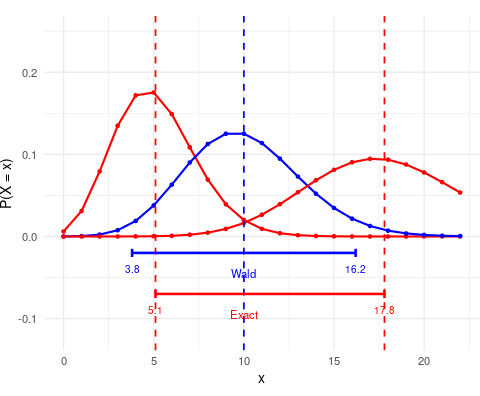
\includegraphics[width=0.64\textwidth]{figures/11-poisson-confidence-intervals.png}
  \caption{Poisson 均值的 Wald 区间与等尾区间（R 绘制）}
  \label{fig:ch11:poisson-ci}
\end{figure}


\end{example}

一种直接的 Bootstrap 方法，称作``\textbf{\emph{正态 Bootstrap 区间}} (normal-bootstrap interval)''，也就是把标准误交给 Bootstrap 估计。用 $B$ 次 Bootstrap 得到 $\widehat\theta_n^{*(1)},\ldots,\widehat\theta_n^{*(B)}$，令 \[ \bar\theta^* =\frac1B\sum_{b=1}^B\widehat\theta_n^{*(b)},\qquad \widehat{\mathrm{se}}_{\mathrm{boot}} =\left\{\frac1{B-1}\sum_{b=1}^B (\widehat\theta_n^{*(b)}-\bar\theta^*)^2\right\}^{1/2} \]正态 Bootstrap 区间为 \[ C_n^{\text{normal boot}} =\left[ \widehat\theta_n-z_{1-\alpha/2}\widehat{\mathrm{se}}_{\mathrm{boot}},\, \widehat\theta_n-z_{\alpha/2}\widehat{\mathrm{se}}_{\mathrm{boot}} \right] \]不过这只是改进了均值和方差 (标准误) 的估计值，仍然是在利用对称的正态分布，没有很好地反映出诸如偏态等高阶信息。

接下来，我们介绍三种进一步的 Bootstrap 置信区间技术，对应三种不同的根 $R(X;\theta)$ 选取策略：
\[\begin{array}{|c|c|c|} \hline \textbf{根} & \textbf{Bootstrap 对应量} & \textbf{区间类型}\\ \hline \widehat\theta_n-\theta & \widehat\theta_n^*-\widehat\theta_n & \text{基础 Bootstrap}\\ \widehat\theta_n & \widehat\theta_n^* & \text{百分位数 (percentile)}\\ \frac{\widehat\theta_n-\theta_0}{\widehat{\mathrm{se}}_n }& \frac{\widehat\theta_n^*-\widehat\theta_n}{\widehat{\mathrm{se}}_n^*} &\text{百分位数-$t$ (percentile-$t$)}\\\hline \end{array}\]
\subsection{基础 Bootstrap 置信区间}

考虑``中心化根''
\[
R_n(\theta_0):=\widehat\theta_n-\theta_0,\qquad R_n^*:=\widehat\theta_n^*-\widehat\theta_n.
\]

令 $r_p^*$ 是 $R_n^*$ 在条件概率 $P^*$ 下的 $p$ 分位数，即
\[r_p^* = \inf\{x:P^*(R_n^*\le x)\ge p\}\]
在实践中，用 $\widehat\theta_n^{*(1)}-\widehat\theta_n,\dots,\widehat\theta_n^{*(B)}-\widehat\theta_n$ 这 $B$ 个数的 $p$ -分位数来代替 $r_p^*$ 。

若 $R_n^*$ 对 $R_n$ 的近似可靠，则
\[P(r_{\alpha/2}^*\le \widehat\theta_n-\theta_0 \le r_{1-\alpha/2}^*)\approx 1-\alpha\]
求解 $\theta_0$ 得到
\[C_n^{\mathrm{basic}} =\left[ \widehat\theta_n-r_{1-\alpha/2}^*,\, \widehat\theta_n-r_{\alpha/2}^* \right]\]
若令 $q_p^*$ 表示 $\widehat\theta_n^*$ 自己的条件 $p$ 分位数，即
\[q_p^* = \inf\{x:P^*(\widehat\theta_n^*\le x)\ge p\}\]
则 $r_p^*=q_p^*-\widehat\theta_n$，同一个区间也可写成
\[C_n^{\mathrm{basic}} =\left[ 2\widehat\theta_n-q_{1-\alpha/2}^*,\, 2\widehat\theta_n- q_{\alpha/2}^* \right]\]
这种方法称作``\textbf{\emph{基础 Bootstrap 置信区间}} (basic bootstrap confidence interval )''。其思想是：

\begin{itemize}
\tightlist
\item
  若 Bootstrap 统计量 $\widehat\theta_n^*$ 高出 $\widehat\theta_n$ ，则说明 $\widehat\theta_n$ 很可能也高出真实参数 $\theta_0$ 。上分位数 $q_{1-\alpha/2}^*$ 描述的是``估计量可能高出中心多少''，因此当它较高时，需要让置信区间左端点往下拉；
\item
  同理，若 Bootstrap 统计量 $\widehat\theta_n^*$ 低于 $\widehat\theta_n$ ，则说明 $\widehat\theta_n$ 可能低于 $\theta_0$ 。下分位数 $q_{\alpha/2}^*$ 描述了``估计量可能低出中心多少''，当它越低时，需要把置信区间右端点向上拉。
\item
  需要注意的是，这种方法对参数的尺度比较敏感。
\end{itemize}

\subsection{百分位 Bootstrap}

\textbf{\emph{百分位区间}} (percentile interval) 直接取 Bootstrap 统计量 $\widehat\theta_n^*$ 的分布计算分位数，令
\[F_n^*(t)=P^*(\widehat\theta_n^*\le t), \qquad q_p^*={F_n^*}^{-1}(p)\]
在实践中，以 $\frac1B\sum_{b=1}^B\mathbb I\Big(\widehat\theta_n^{*(b)}\le t\Big)$ 来代替 $F_n^*(t)$ 。

那么一个 $1-\alpha$ 百分位区间为
\[C_n^{\mathrm{perc}}=\left[q_{\alpha/2}^*,q_{1-\alpha/2}^*\right]\]
也可以写成
\[
C_n^{\mathrm{perc}}
=\left\{\theta:\frac\alpha2\le F_n^*(\theta)\le 1-\frac\alpha2\right\}.
\]
这种方法思路很直接，就是用 Bootstrap 分布来找置信区间；直觉上，诸如偏度等高阶性质，可以体现在 Bootstrap 分布的形状当中，因此百分位区间也可以适应这一点。

如下是 \cite{efronhastie2016} 第 11.2 节的例子，数据原于 22 名学生分别参加两门课程考试的成绩，样本相关系数 $\widehat\theta_n=0.498$ 的取值，使用 $B=2000$ 次经验分布重抽样得到相关系数重复值，用这些数据的 $0.025$ 和 $0.975$ 分位数得到 $[0.118,0.758]$ 的百分位区间。

从图~\ref{fig:ch11:percentile-interval} 中可以明显看出 Bootstrap 统计量分布左偏，并反映到了百分位数区间的端点上：它在 $\widehat\theta_n$ 左侧的部分较长、右侧的部分较短；换言之，百分位区间是允许不对称的，这相比 Wald 置信区间是一个改进。

\begin{figure}[htbp]
  \centering
  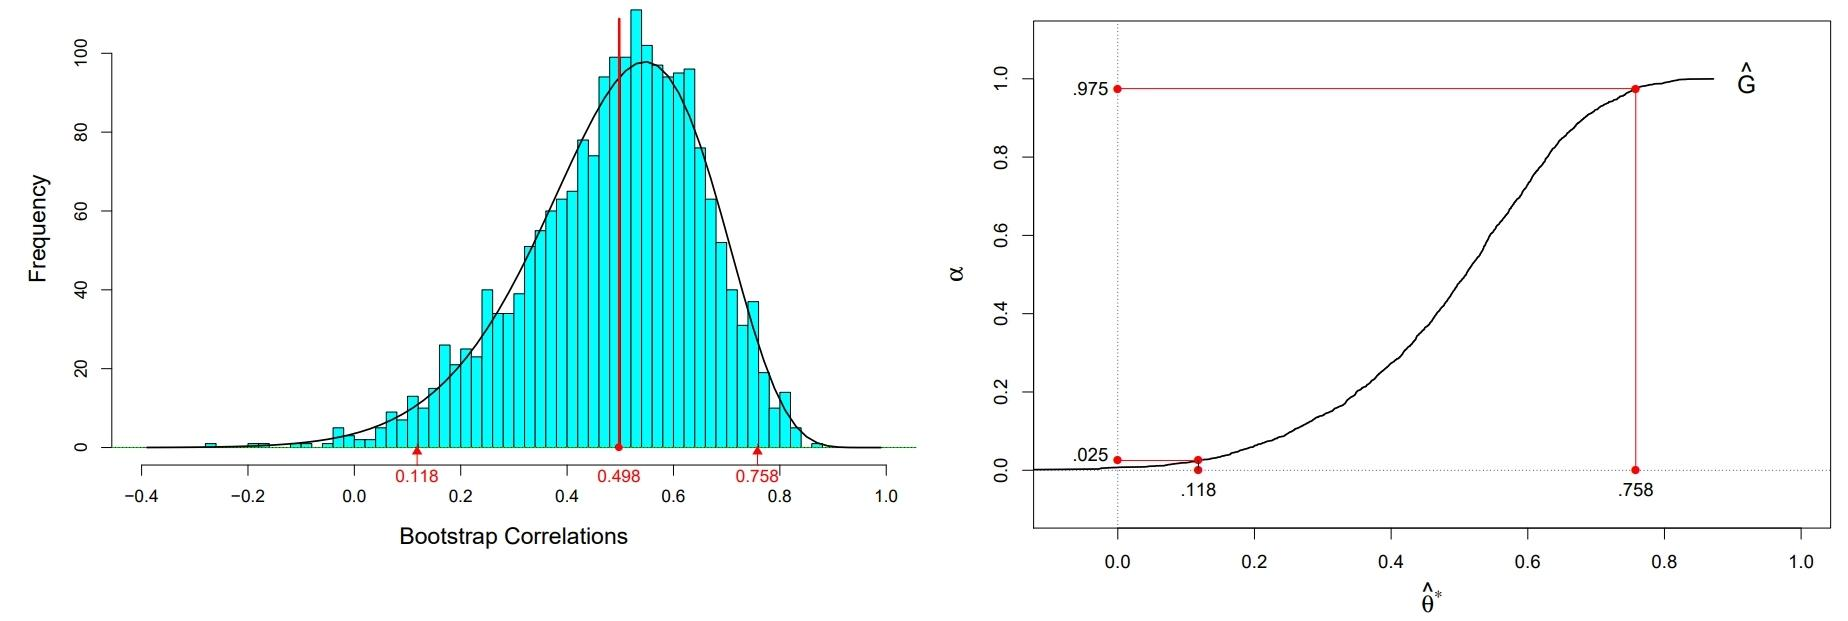
\includegraphics[width=0.94\textwidth]{figures/11-percentile-interval.png}
  \caption{相关系数的 Bootstrap 分布与百分位区间。图片来自 \cite{efronhastie2016}, \S11.2}
  \label{fig:ch11:percentile-interval}
\end{figure}

百分位区间的一个优点是，它在单调变换下保持不变性，这是说，若对参数空间作变换 $\theta\mapsto g(\theta)$ ，且 $g$ 严格递增，则 $g(\widehat\theta_n^*)$ 的 $\gamma$ 分位数就是 $g(q_\gamma^*)$。所以对 $\theta$ 做出的百分位区间，经过 $g$ 变换后，正是对 $g(\theta)$ 直接做百分位区间的结果。

例如上述相关系数的例子中，我们知道 Fisher 变换会把相关系数变到
\[\varphi=\frac12\log\frac{1+\theta}{1-\theta}\]
的尺度上做近似正态推断（见第~\ref{ch:delta-method}~章例~\ref{ex:ch5:fisher-z}）；百分位方法没有显式寻找这样的变换 $\varphi$，仅通过单调变换不变性便复现了这种尺度选择。本文介绍的其他两种 Bootstrap 区间一般不具有这种性质。

一阶正确性的推导非常容易：假设存在 $a_n\to\infty$，使得
\[a_n(\widehat\theta_n-\theta_0)\overset{\rm d}\to Z\]
其中 $Z$ 有\emph{连续且对称的分布函数}， $p$ 分位数记为 $z_p$。那么，若 Bootstrap 能够达到一阶正确：
\[\sup_x\left| P^*(a_n(\widehat\theta_n^*-\widehat\theta_n)\le x) -P(Z\le x) \right|\overset{P}\to 0\]
则
\[a_n(q_p^*-\widehat\theta_n)\overset{P}\to z_p\]
利用
\[\begin{aligned}  &q_{\alpha/2}^*\le \theta_0\le q_{1-\alpha/2}^*\\ \iff\ & a_n(q_{\alpha/2}^*-\widehat\theta_n) \le -a_n(\widehat\theta_n-\theta_0) \le a_n(q_{1-\alpha/2}^*-\widehat\theta_n)\end{aligned}\]
和 $Z$ 的对称性，取极限得到
\[P(\theta_0\in C_n^{\mathrm{perc}})\to P(z_{\alpha/2}\le -Z\le z_{1-\alpha/2}) =1-\alpha,\quad \text{ 当 }n\to\infty\]
不过，我们无法保证二阶准确性：$\widehat\theta_n$ 的分布通常不会是枢轴量，它依赖未知尺度、偏度、偏差和讨厌参数等等。Edgeworth 展开一旦写到 $n^{-1/2}$ 项，这些依赖就会进入分布修正项（ $n^{-1/2}$ 阶项），Bootstrap 未必能把一阶修正项抵消掉，所以覆盖误差经常只有 $O(n^{-1/2})$。为了提高覆盖误差的准确性，当目标是更高阶的覆盖精度，通常需要学生化，或者引入 BCa 这类专门修正端点的办法。

\subsection{学生化 Bootstrap}

记
\[
T_n(\theta_0) =\frac{\widehat\theta_n-\theta_0}{\widehat{\mathrm{se}}_n},\quad T_n^* =\frac{\widehat\theta_n^*-\widehat\theta_n} {\widehat{\mathrm{se}}_n^*}.
\]

若 $c_p$ 是 $T_n(\theta_0)$ 的真实 $p$ 分位数，则
\[P(c_{\alpha/2}\le T_n(\theta_0)\le c_{1-\alpha/2})=1-\alpha\]
反解出 $\theta_0$ 的范围得到理想的置信区间
\[\left[ \widehat\theta_n-c_{1-\alpha/2}\widehat{\mathrm{se}}_n,\, \widehat\theta_n-c_{\alpha/2}\widehat{\mathrm{se}}_n \right]\]
由于 $c_p$ 不可得，因此用 $T_n^*$ 的分位数 $c_p^*={F_n^*}^{-1}(p)$ 估计之，其中 $F_n^*$ 是 $T_n^*$ 的 CDF；在实践中，用
\[
\frac{\widehat\theta_n^{*(1)}-\widehat\theta_n}{\widehat{\mathrm{se}}_n^{*(1)}},
\dots,
\frac{\widehat\theta_n^{*(B)}-\widehat\theta_n}{\widehat{\mathrm{se}}_n^{*(B)}}
\]
的 $p$ 分位数代替 $c_p^*$。学生化 Bootstrap 区间，也叫 \textbf{\emph{百分位-$t$ 区间}}，为
\[C_n^{\mathrm{stud}} =\left[ \widehat\theta_n-c_{1-\alpha/2}^*\widehat{\mathrm{se}}_n,\, \widehat\theta_n-c_{\alpha/2}^*\widehat{\mathrm{se}}_n \right]\]
学生化的好处是，它``比较接近枢轴量''；除以 $\widehat{\mathrm{se}}_n$ 能够消掉尺度的影响，从而使 Bootstrap 捕捉更高阶的信息。回顾本章定理~\ref{thm:ch11:second-order-accuracy}，在适当的光滑性条件下，Bootstrap 能够达到二阶准确：
\[\sup_x \left| P^*(T_n^*\leq x)-P(T_n(\theta_0)\leq x) \right| =O_P(n^{-1})\]
我们希望，Bootstrap 的二阶准确能够推出百分位- $t$ 区间的二阶准确，即
\[P\big(F_n^{*-1}(\alpha/2)\le T_n\le F_n^{*-1}(1-\alpha/2)\big)= 1-\alpha+O(n^{-1})\]
或者简化一些：$c_p^*-c_p=O_P(n^{-1})$ ，也就是说 Bootstrap 分布的准确性能够传导到 Bootstrap 分位数的准确性。这依赖分布函数在分位数处能够足够光滑；在适当光滑性条件满足的时候，这一结论是成立的，请见下一节的 Cornish-Fisher 展开 。

\begin{theorem}[百分位-t 区间的二阶准确]\label{thm:ch11:percentile-t-second-order}

设标量参数 $\theta_0=\theta(P)$ 有估计量 $\widehat\theta_n$，且如下条件满足

\begin{itemize}
\tightlist
\item
  标准误估计满足 $\widehat{\mathrm{se}}_n/\mathrm{se}\overset P\to1$ ，其中 $\mathrm{se}>0$ ；
\item
  学生化统计量 $T_n$ 的分布函数 $F_n(x)=P(T_n\le x)$ 在分位数 $c_{\alpha/2}$ 和 $c_{1-\alpha/2}$ 附近有连续且有界的密度，且该密度在这两个点附近有正下界；
\item
  定理~\ref{thm:ch11:second-order-accuracy} 的光滑性条件成立，包括足够高阶矩存在，且 Edgeworth 二阶展开的 Cramér 条件成立。（此时 Bootstrap 统计量 $T_n^*$ 对 $T_n$ 具有二阶准确性： $\sup_x\left| P^*(T_n^*\le x)-P(T_n\le x) \right|= O_P(n^{-1})$ 。）
\end{itemize}

那么百分位-t 区间满足二阶准确性：
\[P\big(\theta_0\in C_n^{\text{stud}}\big)= 1-\alpha+O(n^{-1})\]
\end{theorem}

\subsection{Cornish-Fisher 展开}
\label{sub:ch11b:cornish-fisher}

定理~\ref{thm:ch11:percentile-t-second-order} 所依赖的结论里，唯一没有完整证明的理论是 Bootstrap 分位数的误差逼近，我们在本节就来进行证明。假设 Edgeworth 展开已经给出了某个 CDF $F_n(x)$ 满足，
\[F_n(x)=\Phi(x)+n^{-1/2}p_1(x)\varphi(x)+n^{-1}p_2(x)\varphi(x)+\cdots\]
我们希望从中反解 $p$ 分位数 $F_n^{-1}(p)$ 能有一个类似的渐近展开形式，形如
\[F_n^{-1}(p)=z_p+n^{-1/2}a_1(z_p)+n^{-1}a_2(z_p)+\cdots\]
其中 $z_p=\Phi^{-1}(p)$ 是标准正态的 $p$ 分位数。

这个反解过程本质上就是逐阶 Taylor 展开，接下来我们简要推导一下二阶的情形。

记 $\epsilon = n^{-1/2}$。考虑一族分布函数 $F_\varepsilon$，它们在标准正态分位数 $z_p$ 的一个邻域内满足一致的 Edgeworth 展开

\begin{equation}
\label{eq:ch11b:tag-6}
F_\epsilon(x) = \Phi(x) + \epsilon\, p_1(x)\varphi(x) + \epsilon^2 p_2(x)\varphi(x) + O(\epsilon^3)
\end{equation}

再假设在该邻域内

\begin{itemize}
\tightlist
\item
  $p_1,p_2$ 二阶连续可微；
\item
  $F_\epsilon$ 具有密度 $F_\epsilon'$ ；
\item
  对充分小的 $\varepsilon$ 存在正常数 $\eta,c$ 使得$\inf_{|x-z_p|\le \eta} F_\epsilon'(x) > c$这保证在 $z_p$ 附近反函数存在且 Lipschitz 连续。
\end{itemize}

我们的目标是对分位数 $x_{p,\epsilon}:=F_\epsilon^{-1}(p)$ 求出形如
\[x_{p,\epsilon} = z_p + \epsilon A + \epsilon^2 B + O(\epsilon^3)\]
的展开式，其中 $A,B$ 是待定的系数。记 $\delta = x - z_p = \epsilon A + \epsilon^2 B$，在 $z_p$ 处展开 $\Phi,\phi,p_1,p_2$：
\[\begin{aligned} \Phi(z_p+\delta) &= \Phi(z_p) + \varphi(z_p)\delta - \frac12 z_p \varphi(z_p)\delta^2 + O(\delta^3)\\ \varphi(z_p+\delta) &= \varphi(z_p)\bigl(1 - z_p\delta + O(\delta^2)\bigr) \end{aligned}\]\[\begin{aligned} p_1(z_p+\delta) &= p_1(z_p) + p_1'(z_p)\delta + O(\delta^2) \\ p_2(z_p+\delta) &= p_2(z_p) + O(\delta) \end{aligned}\]
然后逐项代入 式~\eqref{eq:ch11b:tag-6}。

\begin{itemize}
\tightlist
\item
  对 $\Phi(x)$ 项：
\end{itemize}
\[\begin{aligned} \Phi(x)=p+\varphi(z_p)\delta - \frac12 z_p \varphi(z_p)\delta^2  \end{aligned}\]
再将 $\delta = \epsilon A + \epsilon^2 B$ 代入，得到
\[\begin{aligned} \Phi(x)=p+ \varphi(z_p)(\epsilon A + \epsilon^2 B)-\frac12 z_p\varphi(z_p) \epsilon^2 A^2 + O(\epsilon^3) \end{aligned}\]
\begin{itemize}
\tightlist
\item
  对 $\epsilon$ 阶项：
  \[  \begin{aligned} \epsilon\, p_1(x)\varphi(x) &= \epsilon\, \varphi(z_p+\delta)\bigl(p_1(z_p)+p_1'(z_p)\delta + O(\delta^2)\bigr) \\ &= \epsilon\,\varphi(z_p)\bigl(1 - z_p\delta + O(\delta^2)\bigr) \bigl(p_1(z_p)+p_1'(z_p)\delta + O(\delta^2)\bigr) \\ &= \epsilon\,\varphi(z_p)\Bigl( p_1(z_p) + \delta\bigl(p_1'(z_p)-z_p p_1(z_p)\bigr) \Bigr) + O(\epsilon\delta^2). \end{aligned}
  \]  代入 $\delta = \epsilon A+O(\epsilon^2)$，我们得到
  \[  \epsilon\, p_1(x)\varphi(x) = \varphi(z_p)\Bigl( \epsilon p_1(z_p) + \epsilon^2 A\bigl(p_1'(z_p)-z_p p_1(z_p)\bigr) \Bigr) + O(\epsilon^3).
  \]\item
  对 $\epsilon^2$ 阶项：
  \[
  \epsilon^2 p_2(x)\varphi(x) = \epsilon^2 p_2(z_p)\varphi(z_p) + O(\epsilon^3).
  \]
\end{itemize}

将上面三部分加起来，则式~\eqref{eq:ch11b:tag-6} 可改写成：
\[\begin{aligned} F_\epsilon(x) - p &= \varphi(z_p)(\epsilon A + \epsilon^2 B)-\frac12 z_p\varphi(z_p) \epsilon^2 A^2 \\ &\quad + \varphi(z_p)\Bigl( \epsilon p_1(z_p) + \epsilon^2 A\bigl(p_1'(z_p)-z_p p_1(z_p)\bigr) \Bigr) \\ &\quad + \epsilon^2 p_2(z_p)\varphi(z_p) + O(\epsilon^3)\\ &= \varphi(z_p)\Bigl( \epsilon\bigl(A + p_1(z_p)\bigr) \\ &\quad +\epsilon^2\Bigl( B - \frac12 z_p A^2 + A\bigl(p_1'(z_p)-z_p p_1(z_p)\bigr) + p_2(z_p) \Bigr) \Bigr) + O(\epsilon^3). \end{aligned}\]选取 $A,B$ 使得 $F_\epsilon(x)=p+O(\epsilon^3)$，即上式中 $\epsilon$ 和 $\epsilon^2$ 的系数为零。

\begin{itemize}
\tightlist
\item
  一阶项：$A + p_1(z_p) = 0$，立即得到 \[A = -p_1(z_p)\]\item
  二阶项：代入 $A$，令 $\epsilon^2$ 的系数为零：
\end{itemize}
\[\begin{aligned} & B = \frac12 z_p A^2 - A\bigl(p_1'(z_p)-z_p p_1(z_p)\bigr) - p_2(z_p)\\ \implies &B= p_1(z_p)p_1'(z_p) - \frac12 z_p\, p_1(z_p)^2 - p_2(z_p) \end{aligned}\]
由此我们得到一个``近似分位数''：

\begin{equation}
\label{eq:ch11b:tag-7}
\widetilde{x}_{p,\epsilon} = z_p - \epsilon p_1(z_p) + \epsilon^2\Bigl( p_1(z_p)p_1'(z_p) - \frac12 z_p p_1(z_p)^2 - p_2(z_p) \Bigr)
\end{equation}

它满足 $F_\epsilon(\widetilde{x}_{p,\epsilon}) = p + O(\epsilon^3)$。

用 $\widetilde{x}_{p,\epsilon} \to z_p$（当 $\epsilon\to0$），真实分位数 $x_{p,\epsilon}$ 也落在该邻域内。由微分中值定理，
\[c\,|x_{p,\epsilon} - \widetilde{x}_{p,\epsilon}|\le |F_\epsilon(x_{p,\epsilon}) - F_\epsilon(\widetilde{x}_{p,\epsilon})|=|\,p - F_\epsilon(\widetilde{x}_{p,\epsilon})\,|=O(\epsilon^3)\]
即 $x_{p,\epsilon} = \widetilde{x}_{p,\epsilon} + O(\epsilon^3)$ ；所以式~\eqref{eq:ch11b:tag-7} 就是我们想要的展开，它称作 \textbf{\emph{Cornish-Fisher 展开}} 。

写作定理：

\begin{theorem}[二阶 Cornish-Fisher 展开]

令 $z_p=\Phi^{-1}(p)$，设分布函数 $F_n$ 在 $z_p$ 附近密度存在有正的下界，且 $F_n$ 有二阶 Edgeworth 展开
\[F_n(x)=\Phi(x)+n^{-1/2}p_1(x)\varphi(x)+n^{-1}p_2(x)\varphi(x)+O(n^{-3/2})\]
其中余项在 $z_p$ 的某邻域内一致成立，且 $F_n$ 在该邻域内严格递增。那么， $F_n^{-1}(p)$ 满足
\[F_n^{-1}(p) = z_p -n^{-1/2}p_1(z_p) +n^{-1} \left( p_1(z_p)p_1'(z_p) -\frac12 z_p p_1(z_p)^2 -p_2(z_p) \right) +O(n^{-3/2})\]
简而言之概括：只要分布函数在 $p$ 分位数附近足够光滑，那么 Edgeworth 展开有多精确， Cornish-Fisher 展开就有多精确。

将之用于 Bootstrap 分布 ${F_n^*}^{-1}(p)$ ：在定理~\ref{thm:ch11:second-order-accuracy} 的条件下， $T_n^*$ 和 $T_n(\theta_0)$ 有 Edgeworth 展开：
\[\begin{aligned} P(T_n(\theta_0)\le x) &= \Phi(x)+n^{-1/2}p_1(x;P)\varphi(x)  +O_P(n^{-1})\\ P^*(T_n^*\le x) &= \Phi(x)+n^{-1/2}p_1(x;\mathbb P_n)\varphi(x) +O_P(n^{-1}) \end{aligned}\]
且 $p_1(x;P)-p_1(x;\mathbb P_n)=O_P(n^{-1/2})$ ，那么 Cornish-Fisher 展开给出
\[\begin{aligned} & \begin{aligned} c_p &= z_p-n^{-1/2} p_1(z_p;P) +O(\epsilon^2)\\ c^*_p &= z_p-n^{-1/2}p_1(z_p;\mathbb P_n) +O(\epsilon^2) \end{aligned}\\ \implies\ & c_p-c_p^*=-n^{-1/2}\big(p_1(z_p;P) -p_1(z_p;\mathbb P_n) \big)+O_P(n^{-1}) =O_P(n^{-1}) \end{aligned}\]
这就是定理~\ref{thm:ch11:percentile-t-second-order} 所需要的结论。

\end{theorem}

这种技术来自于 \cite{hall1986}；读者也可以参考 \cite{hall1992} 一书。

\subsection{偏差校正与 BCa 区间}

众所周知，Bootstrap 也能估计偏差：
\[\widehat{\mathrm{bias}}_{\mathrm{boot}} =\mathbb E^*[\widehat\theta_n^*]-\widehat\theta_n \approx \frac1B\sum_{b=1}^B\widehat\theta_n^{*(b)} -\widehat\theta_n\]
因此对一个点估计 $\widehat\theta_n$ ，我们可以写出它的偏差校正：
\[\widehat\theta_n^{\mathrm{bc}} =\widehat\theta_n-\widehat{\mathrm{bias}}_{\mathrm{boot}}\]
当然，点估计的偏差校正不能自动变成好的置信区间。我们要的实际上是校正``中位偏差 (median bias)''：若 Bootstrap 分布已经围绕 $\widehat\theta_n$ 是对称的，那么应有 $P^*(\widehat\theta_n^*\le \widehat\theta_n)\approx \tfrac12$ 。实际数据会告诉我们这个比例是否偏离 $\tfrac12$：令
\[
\widehat p_0 = P^*(\widehat\theta_n^*\le \widehat\theta_n) \approx \frac1B\sum_{b=1}^B\mathbb I\Big(\widehat\theta_n^{*(b)}\le \widehat\theta_n\Big).
\]

并定义偏差校正常数
\[\widehat z_0:=\Phi^{-1}(\widehat p_0)\]
$\widehat z_0=0$ 对应 Bootstrap 分布以 $\widehat\theta_n$ 为中位中心；$\widehat z_0<0$ 表示少于一半的 Bootstrap 重复值落在 $\widehat\theta_n$ 左边，Bootstrap 重复值整体偏高，区间端点通常要往低调整；$\widehat z_0>0$ 则相反。

BC-百分位 (BC-percentile) 方法直接修改百分位区间的概率截点。仍记 $F_n^*(t)=P^*(\widehat\theta_n^*\le t)$ 、 $q_p^*=(F_n^*)^{-1}(p)$ 、 $z_p=\Phi^{-1}(p)$ ；对名义水平 $p$ ，BC-百分位方法使用 $\Phi(2\widehat z_0+z_{p})$ 作为新的 Bootstrap 分位数水平，那么名义 $1-\alpha$ 的 BC-百分位区间为
\[C_n^{\text{BC}}=\Big[{F_n^*}^{-1}(\Phi(2\widehat z_0+z_{\alpha/2})),{F_n^*}^{-1}(\Phi(2\widehat z_0+z_{1-\alpha/2}))\Big]\]
简而言之： 若 $\widehat z_0\ne0$，说明 Bootstrap 分布的中位中心没有落在 $\widehat\theta_n$，BC-百分位把正态分位数刻度以 $\widehat z_0$ 为中心作平移校正， $z_p$ 被替换为 $2\widehat z_0+z_p$ 。若 $\widehat z_0=0$，BC-百分位退回普通百分位区间。

BC-百分位仍然只校正中位偏差。若标准误在参数尺度上变化，单靠 $\widehat z_0$ 不够。BCa 方法在 BC 的基础上引入加速常数 $\widehat a$ ，通过额外的影响函数或者 jackknife 方法从样本中计算获得，然后以 $\Phi\left( \widehat z_0+ \frac{\widehat z_0+z_p} {1-\widehat a(\widehat z_0+z_p)} \right)$ 作为新的 Bootstrap 分位数水平。可以说 BCa 使用了多达三重的校正：分位数 Bootstrap 校正分布近似、 $\widehat z_0$ 校正偏差、 $\widehat a$ 校正标准误；这也使得该方法能够达到二阶的准确。

我们对此不作更多介绍，可以参考 \cite{efron1987}。

\begin{example}[指数分布的置信区间比较]\label{ex:ch11:exponential}

设从指数分布 (尺度参数化) $\mathrm{Exp}(\theta)$ 中抽取出 $n=5$ 的样本，记样本均值为 $\widehat\theta$ ，图~\ref{fig:ch11:ci-exponential} 展示了精确置信区间、分位数区间、BC、BCa 四种置信区间的左右端点 $L\widehat\theta,U\widehat\theta$ ，以及各自的尾部面积 $P(L\widehat\theta>\theta)$ 和 $P(U\widehat\theta<\theta)$(图中称作错误率，\%) 。

\begin{figure}[htbp]
  \centering
  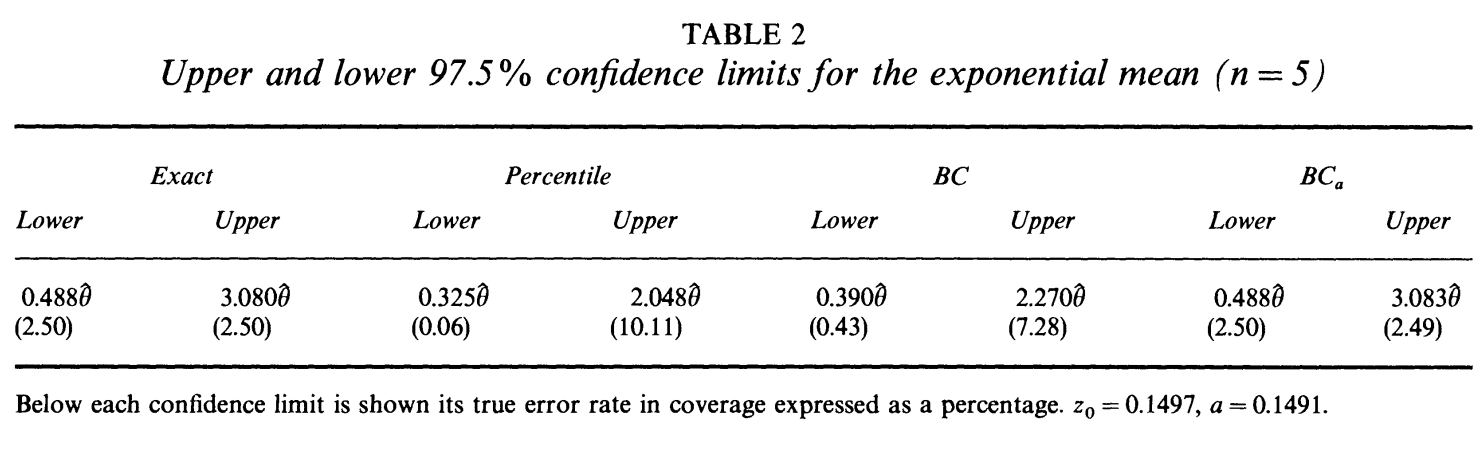
\includegraphics[width=0.96\textwidth]{figures/11-confidence-interval-comparison.png}
  \caption{指数分布均值的四种置信区间比较。图片来自 \cite{diciccioromano1988}}
  \label{fig:ch11:ci-exponential}
\end{figure}

其中，

\begin{itemize}
\tightlist
\item
  精确的 95\% 置信区间可以利用枢轴量 $\tfrac{2n\widehat\theta}{\theta}\sim\chi_{2n}^2$ 得出： $\left[\frac{2n\widehat\theta}{\chi^2_{2n}(0.975)},\frac{2n\widehat\theta}{\chi^2_{2n}(0.025)}\right]$ ；
\item
  使用参数 Bootstrap ，则应用 $\mathrm{Exp}(1/\widehat\theta)$ 代替样本分布；本例中不需要真的 Monte Carlo 重抽样，只需要再次利用枢轴量，即可用 χ² 分布的分位数得到各 Bootstrap 区间。例如，令 $q_p$ 代表 $\chi^2_{2n}$ 的 $p$ 分位数，则百分位区间为 $\left[\tfrac{q_{0.025}}{2n}\widehat\theta,\tfrac{q_{0.975}}{2n}\widehat\theta\right]$ 。
\end{itemize}

下面是一个稍微复杂一些的例子，取 $X\sim \mathrm{Exp}(1/\eta^1)$ 、 $Y\sim\mathrm{Gamma}(c,1/\eta^2)$ ， $\theta=\eta^2/\eta^1$ ，其中 $c=0.4$ 。仍取 $n=5$ 个样本， $\widehat\theta=\frac{\widehat\eta^2}{\widehat\eta^1}=\frac{c\sum_{j=1}^5 X_j}{\sum_{j=1}^5Y_j}$ 是 $\eta^2$ 和 $\eta^1$ 的 MLE 之比。四种置信区间的比较见图~\ref{fig:ch11:ci-ratio}。

\begin{figure}[htbp]
  \centering
  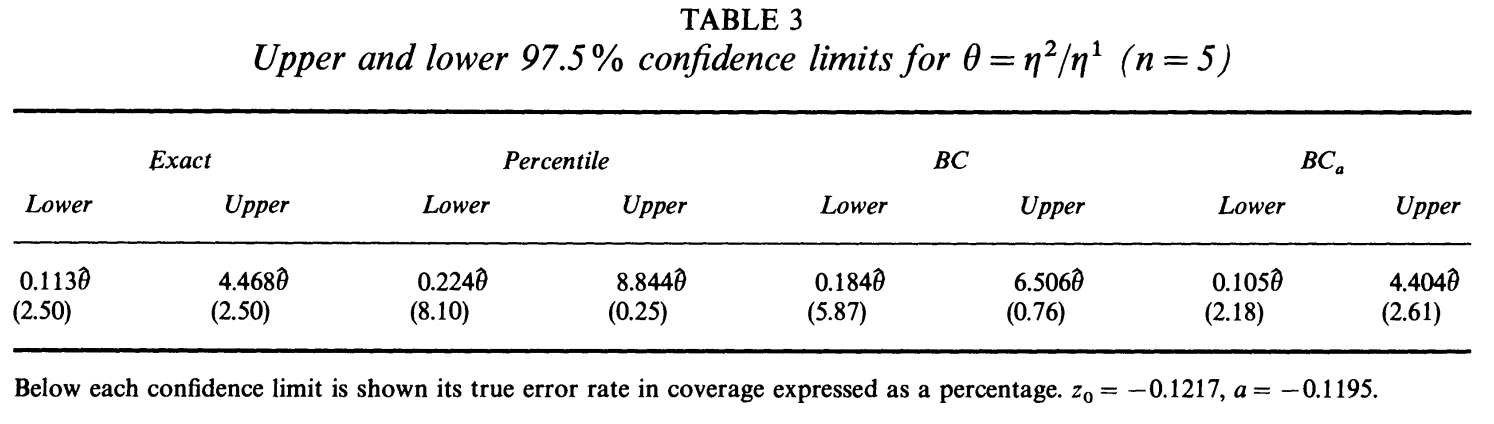
\includegraphics[width=0.96\textwidth]{figures/11-ratio-confidence-interval-comparison.png}
  \caption{两参数比值的四种置信区间比较。图片来自 \cite{diciccioromano1988}}
  \label{fig:ch11:ci-ratio}
\end{figure}

精确的 95\% 置信区间可以利用枢轴量 $\tfrac{\widehat\theta}{\theta}\sim F_{2n,2nc}$ 算出。

这两个例子中，普通百分位区间和 BC 区间的两侧错误率明显不平衡，而 BCa 区间几乎与精确区间一致。


\end{example}

\section{关于 Bootstrap 的补充}

\subsection{失效}

Bootstrap 不是在任何情况下都可以随便用的------虽然它在很多时候都非常方便且好用，但其\emph{正当性必须由其渐近结构来保证}。如果正则条件不满足，完全可以构造 Bootstrap 失效的例子。这些例子包括

\begin{itemize}
\tightlist
\item
  统计泛函 $\theta(P)$ 不光滑；
\item
  $\widehat\theta_n$ 逼近 $\theta_0$ 的速率不是标准的 $O_P(n^{-1/2})$ ，那么重抽样样本与原始样本量相同的`` $n$ -out-of- $n$ '' Bootstrap 是不适用的；
\item
  参数落在支撑集合的边界上，或者统计量依赖于分布极值或支撑边界，如样本极值；见下面的例~\ref{ex:ch11:extreme}。
\item
  对相依数据使用 i.i.d. Bootstrap：例如 $X_j$ 是时间序列，那么从 $\mathbb P_n$ i.i.d. 抽样显然会破坏自相关结构。
\item
  模型选择或者 post-selection 估计量。
\end{itemize}

% \href{https://stats.stackexchange.com/questions/9664/what-are-examples-where-a-naive-bootstrap-fails}{What are examples where a ``naive bootstrap'' fails? - Cross Validated}

\cite{chernick2011} 一书的第 9 章就深入讨论了各种 Bootstrap 失效的情形。我们举一个最简单的例子：

\begin{example}[样本极值]
\label{ex:ch11:extreme}
设
\[X_1,\ldots,X_n\sim \mathcal{U}(0,\theta)\quad \text{i.i.d.}, \qquad \widehat\theta_n=X_{(n)}=\max_i X_i\]
不难证明 $\widehat\theta_n$ 真实极限为
\[n(\theta-X_{(n)})\overset{\rm d}\to \mathrm{Exp}(\theta)\]
Bootstrap 最大值 $X_{(n)}^*$ 从原样本中重抽；以原始数据为条件，Bootstrap 样本包含原最大值 $X_{(n)}$ 的概率是
\[P^*(X_{(n)}^*=X_{(n)}) =1-\left(1-\frac1n\right)^n \to 1-e^{-1}\]
因此 $n\big(X_{(n)}-X_{(n)}^*\big)$ 在 $0$ 处保留一个约 $1-e^{-1}$ 的原子概率，而真实极限是连续的指数分布。一个带固定的原子概率的条件分布，显然是不可能依分布收敛到指数分布的。


\end{example}

例~\ref{ex:ch11:extreme} 的问题在于，经验分布很难捕捉极值 $X_{(n)}$ 这一信息，每次重抽样可能完全抽不到 $X_{(n)}$ 。如果从参数的角度出发，$\theta$ 位于支撑集的边界上，也可视作造成问题的原因；若将 $\theta$ 视作统计泛函 $\mathcal U(0,\theta)\mapsto \theta$ ，它在某些方向上甚至不存在有限的 Gâteaux 导数，自然不会满足定理~\ref{cor:ch11:functional-delta-normality} 的条件。

还有要注意的是，就算 Bootstrap 能满足一阶正确性，二阶准确性也可能失效。回顾定理~\ref{thm:ch11:second-order-accuracy}，要保证 Bootstrap 二阶准确性，至少需要

\begin{itemize}
\tightlist
\item
  统计量足够光滑；
\item
  有足够阶矩存在；
\item
  Edgeworth 展开所需的 Cramér 条件；
\item
  如果 Bootstrap 过程需估计讨厌参数，它们必须有足够好的相合估计；
\item
  统计量是渐近枢轴量。
\end{itemize}

总之，一阶有效 $\nRightarrow$ 二阶准确。

\subsection{变体}

由于上述各种例外情况，我们介绍的一般 Bootstrap 也有很多不同的变体；关键问题是：如何使用现有的样本得到一个``能够很好近似目标样本分布''的分布，而这基本都是从重抽样方案出发进行改进。如下：
\[\begin{array}{|c|c|}\hline \textbf{问题结构} & \text{Bootstrap 变体}\\ \hline \text{有可信的参数模型 }P_\theta & \text{参数 Bootstrap}\\ \hline \text{有光滑的密度} & \substack{\displaystyle\text{光滑 Bootstrap}\\ \displaystyle\text{(Smoothed Bootstrap)}}\\ \hline \text{非标准收敛速率/边界} & \substack{\displaystyle \text{ $m$-out-of-$n$ Bootstrap,}\\ \displaystyle\text{子采样 (Subsampling)}}\\ \hline \text{异方差回归}& \text{Wild Bootstrap}\\ \hline \text{时间序列或空间相关} & \substack{\displaystyle\text{分块 Bootstrap}\\ \displaystyle\text{(Block Bootstrap)}}\\ \hline \text{高维经验过程} & \substack{\displaystyle\text{乘子 Bootstrap}\\ \displaystyle\text{(Multiplier Bootstrap)}}\\ \hline \end{array}\]
这些方法各自对应一种结构判断：

\begin{itemize}
\tightlist
\item
  参数 Bootstrap 已在本章前文介绍：如果参数族模型正确，那么参数 Bootstrap 往往能够得到效率更高的估计。
\item
  光滑 Bootstrap 类似：如果我们已知``目标样本分布有光滑的密度''，那么可以将重抽样的分布平滑一下，例如核平滑 (Kernel Smoothing)，再来用于近似目标分布，这样也可能提高估计效率，并且避免了``只能从已知样本中重抽样，导致经常抽出重复值''的问题。见 \cite{silvermanyoung1987}。
\item
  如果 $\widehat\theta_n$ 收敛于 $\theta$ 的速度比 $O_P(n^{-1/2})$ 更快，比如例~\ref{ex:ch11:extreme} 是按照 $O_P(n^{-1})$ 速度，那么就不能再简单地让重抽样样本与原始样本量相同，考虑 $\text{$m$-out-of-$n$}$ Bootstrap，每次重抽样只抽取 $m$ 次，其中 $m/n\to 0$ 、 $m\to\infty$ ，例如可以取 $m=\sqrt n$ 。这样，Bootstrap 样本的极端值行为与真实抽样更匹配。参数位于边界的情况同理。
\item
  子采样 (subsampling) 由 \cite{politisromano1994} 系统提出。简而言之，其思路是运行很多次重采样，采样次数 $m$ 远小于 $n$ （同样 $m/n\to 0$ 、 $m\to\infty$ ），但与 $\text{$m$-out-of-$n$}$ Bootstrap 不同的是，这里的重采样是\emph{无放回}的。子采样的正确性可以在非常弱的条件下成立，不需要 Bootstrap 那样的光滑性条件；对于有依赖的时间序列数据，子采样也可以使用，总之是一种比较强大的方法。进一步可参考 \cite{politisromanowolf1999}。
\item
  Wild Bootstrap 已在本章例~\ref{ex:ch11:wild-bootstrap} 中介绍。
\item
  如果数据存在序列相关或空间相关，独立重抽样会打乱相依结构，这种情况下可以用分块 Bootstrap。例如对平稳离散时间序列就把相邻 $l$ 个时间的 $X_t$ 放在同一个块中（允许块间重叠），然后以块为单位进行重抽样，再把重抽样块拼到一起，这种方法来自 \cite{kunsch1989}。
\item
  乘子 Bootstrap ( multiplier bootstrap) 的思想是生成辅助随机变量 $w_1,\dots,w_n$ ，从而构造随机加权的经验过程 $\mathbb G_n^wf=\frac1{\sqrt n}\sum_{j=1}^nw_j(f(X_j)-Pf)$ 。这个理论比较复杂，不多赘述。
\end{itemize}

最后，我们以一个 $\text{$m$-out-of-$n$}$ Bootstrap的例子作为结尾。

\begin{example}[$m$-out-of-$n$ 的极值例]
\label{ex:ch11:m-out-of-n}

设 $m\to\infty$，且 $m/n\to 0$。定义 bootstrap 统计量
\[T_{n,m}^* = m\big(X_{(n)}-X_{(m)}^*\big)\]
其中 $X_{(m)}^*$ 是从经验分布中有放回抽取 $m$ 个样本的最大值。显见， \[ P^*(T_{n,m}^*=0)=P^*\big(X_{(n)}=X_{(m)}^*\big)=1-\left(1-\frac1n\right)^m=\frac mn+o\left(\frac mn\right)\to 0 \]所以之前``在 0 处总存在原子概率''的问题完全被解决了。

对任意固定的 $t \ge 0$，
\[ \begin{aligned} P^*\bigl(T_{n,m}^* > t\bigr) &= P^*\left(X_{(m)}^* < X_{(n)} - \frac{t}{m}\right) \\ &= \left(\mathbb F_n\!\left(X_{(n)} - \frac{t}{m}\right)\right)^m \\ &=\left(1-\frac {N_{n,t}}n\right)^m \end{aligned} \]其中 $N_{n,t} := \#\left\{i : X_i > X_{(n)} - \tfrac{t}{m}\right\}$ 。

给定 $X_{(n)}$ 时，其余 $n-1$ 个样本点独立地服从 $\mathcal{U}(0, X_{(n)})$，落入区间 $\bigl(X_{(n)} - \frac{t}{m},\, X_{(n)}\bigr]$ 的概率为 $\tfrac{t/m}{X_{(n)}}$，因此
\[N_{n,t} - 1 \mid X_{(n)} \;\sim\; \mathrm{Binomial}\left(n-1,\; \frac{t}{m X_{(n)}}\right)\]
得
\[\begin{aligned} \mathbb{E}\left[\frac{m N_{n,t}}{n} \ \bigg|\  X_{(n)}\right] &=\frac{m}{n}+\frac{m(n-1)}{n}\frac{t}{m X_{(n)}} \overset P\to \frac{t}{\theta}\\  \mathrm{Var}\left[\frac{m N_{n,t}}{n} \ \bigg|\  X_{(n)}\right] &= \frac{m^2}{n^2}(n-1)\frac{t}{m X_{(n)}}\left(1-\frac{t}{m X_{(n)}}\right) = O\left(\frac{m}{n}\right) \to 0  \end{aligned}\]
这推出 $\tfrac{mN_{n,t}}{n}\overset{P}\to\tfrac t\theta$ ，利用这一点，以及 $\tfrac{N_{n,t}}{n}=O_{P}\left(\tfrac1m\right)$ ，最终得到
\[P^*\bigl(T_{n,m}^* > t\bigr) = \exp\!\left\{m\log\!\left(1 - \frac{N_{n,t}}{n}\right)\right\}=\exp\left\{-\frac {mN_{n,t}}{n}+O_{P}\left(\frac 1m\right)\right\} \overset{P}\longrightarrow e^{-t/\theta}\]
这就证明了 $T_{n,m}^*\overset{\rm d^*}\to\mathrm{Exp}(\theta)$ ，且由条件版本的 Pólya 定理，
\[\sup_x \bigl| P^*(T_{n,m}^* \le x) - P(\mathrm{Exp}(\theta) \le x) \bigr| \xrightarrow{P} 0\]
\end{example}


\nocite{efron1979,efrontibshirani1993,hall1992}
\chapterreferences
\end{refsection}

\end{document}
